\documentclass[a4paper,12pt,twoside,onecolumn,openright,final,oldfontcommands]{memoir}
\usepackage{lmodern}
\usepackage{amssymb,amsmath}
\usepackage{ifxetex,ifluatex}
\usepackage{fixltx2e} % provides \textsubscript
\ifnum 0\ifxetex 1\fi\ifluatex 1\fi=0 % if pdftex
  \usepackage[T1]{fontenc}
  \usepackage[utf8]{inputenc}
\else % if luatex or xelatex
  \ifxetex
    \usepackage{mathspec}
  \else
    \usepackage{fontspec}
  \fi
  \defaultfontfeatures{Ligatures=TeX,Scale=MatchLowercase}
\fi
% use upquote if available, for straight quotes in verbatim environments
\IfFileExists{upquote.sty}{\usepackage{upquote}}{}
% use microtype if available
\IfFileExists{microtype.sty}{%
\usepackage{microtype}
\UseMicrotypeSet[protrusion]{basicmath} % disable protrusion for tt fonts
}{}
\usepackage{hyperref}
\hypersetup{unicode=true,
            pdftitle={Understanding rumination as a form of inner speech},
            pdfborder={0 0 0},
            breaklinks=true}
\urlstyle{same}  % don't use monospace font for urls
\usepackage{color}
\usepackage{fancyvrb}
\newcommand{\VerbBar}{|}
\newcommand{\VERB}{\Verb[commandchars=\\\{\}]}
\DefineVerbatimEnvironment{Highlighting}{Verbatim}{commandchars=\\\{\}}
% Add ',fontsize=\small' for more characters per line
\newenvironment{Shaded}{}{}
\newcommand{\AlertTok}[1]{\textcolor[rgb]{1.00,0.00,0.00}{\textbf{#1}}}
\newcommand{\AnnotationTok}[1]{\textcolor[rgb]{0.38,0.63,0.69}{\textbf{\textit{#1}}}}
\newcommand{\AttributeTok}[1]{\textcolor[rgb]{0.49,0.56,0.16}{#1}}
\newcommand{\BaseNTok}[1]{\textcolor[rgb]{0.25,0.63,0.44}{#1}}
\newcommand{\BuiltInTok}[1]{#1}
\newcommand{\CharTok}[1]{\textcolor[rgb]{0.25,0.44,0.63}{#1}}
\newcommand{\CommentTok}[1]{\textcolor[rgb]{0.38,0.63,0.69}{\textit{#1}}}
\newcommand{\CommentVarTok}[1]{\textcolor[rgb]{0.38,0.63,0.69}{\textbf{\textit{#1}}}}
\newcommand{\ConstantTok}[1]{\textcolor[rgb]{0.53,0.00,0.00}{#1}}
\newcommand{\ControlFlowTok}[1]{\textcolor[rgb]{0.00,0.44,0.13}{\textbf{#1}}}
\newcommand{\DataTypeTok}[1]{\textcolor[rgb]{0.56,0.13,0.00}{#1}}
\newcommand{\DecValTok}[1]{\textcolor[rgb]{0.25,0.63,0.44}{#1}}
\newcommand{\DocumentationTok}[1]{\textcolor[rgb]{0.73,0.13,0.13}{\textit{#1}}}
\newcommand{\ErrorTok}[1]{\textcolor[rgb]{1.00,0.00,0.00}{\textbf{#1}}}
\newcommand{\ExtensionTok}[1]{#1}
\newcommand{\FloatTok}[1]{\textcolor[rgb]{0.25,0.63,0.44}{#1}}
\newcommand{\FunctionTok}[1]{\textcolor[rgb]{0.02,0.16,0.49}{#1}}
\newcommand{\ImportTok}[1]{#1}
\newcommand{\InformationTok}[1]{\textcolor[rgb]{0.38,0.63,0.69}{\textbf{\textit{#1}}}}
\newcommand{\KeywordTok}[1]{\textcolor[rgb]{0.00,0.44,0.13}{\textbf{#1}}}
\newcommand{\NormalTok}[1]{#1}
\newcommand{\OperatorTok}[1]{\textcolor[rgb]{0.40,0.40,0.40}{#1}}
\newcommand{\OtherTok}[1]{\textcolor[rgb]{0.00,0.44,0.13}{#1}}
\newcommand{\PreprocessorTok}[1]{\textcolor[rgb]{0.74,0.48,0.00}{#1}}
\newcommand{\RegionMarkerTok}[1]{#1}
\newcommand{\SpecialCharTok}[1]{\textcolor[rgb]{0.25,0.44,0.63}{#1}}
\newcommand{\SpecialStringTok}[1]{\textcolor[rgb]{0.73,0.40,0.53}{#1}}
\newcommand{\StringTok}[1]{\textcolor[rgb]{0.25,0.44,0.63}{#1}}
\newcommand{\VariableTok}[1]{\textcolor[rgb]{0.10,0.09,0.49}{#1}}
\newcommand{\VerbatimStringTok}[1]{\textcolor[rgb]{0.25,0.44,0.63}{#1}}
\newcommand{\WarningTok}[1]{\textcolor[rgb]{0.38,0.63,0.69}{\textbf{\textit{#1}}}}
\usepackage{longtable,booktabs}
\usepackage{graphicx,grffile}
\makeatletter
\def\maxwidth{\ifdim\Gin@nat@width>\linewidth\linewidth\else\Gin@nat@width\fi}
\def\maxheight{\ifdim\Gin@nat@height>\textheight\textheight\else\Gin@nat@height\fi}
\makeatother
% Scale images if necessary, so that they will not overflow the page
% margins by default, and it is still possible to overwrite the defaults
% using explicit options in \includegraphics[width, height, ...]{}
\setkeys{Gin}{width=\maxwidth,height=\maxheight,keepaspectratio}
\IfFileExists{parskip.sty}{%
\usepackage{parskip}
}{% else
\setlength{\parindent}{0pt}
\setlength{\parskip}{6pt plus 2pt minus 1pt}
}
\setlength{\emergencystretch}{3em}  % prevent overfull lines
\providecommand{\tightlist}{%
  \setlength{\itemsep}{0pt}\setlength{\parskip}{0pt}}
\setcounter{secnumdepth}{5}
% Redefines (sub)paragraphs to behave more like sections
\ifx\paragraph\undefined\else
\let\oldparagraph\paragraph
\renewcommand{\paragraph}[1]{\oldparagraph{#1}\mbox{}}
\fi
\ifx\subparagraph\undefined\else
\let\oldsubparagraph\subparagraph
\renewcommand{\subparagraph}[1]{\oldsubparagraph{#1}\mbox{}}
\fi

%%% Use protect on footnotes to avoid problems with footnotes in titles
\let\rmarkdownfootnote\footnote%
\def\footnote{\protect\rmarkdownfootnote}

%%% Change title format to be more compact
\usepackage{titling}

% Create subtitle command for use in maketitle
\providecommand{\subtitle}[1]{
  \posttitle{
    \begin{center}\large#1\end{center}
    }
}

\setlength{\droptitle}{-2em}

  \title{Understanding rumination as a form of inner speech}
    \pretitle{\vspace{\droptitle}\centering\huge}
  \posttitle{\par}
    \author{}
    \preauthor{}\postauthor{}
    \date{}
    \predate{}\postdate{}
  
%%%%%%%%%%%%%%%%%%%%%%%%%%%%%
% Loading relevant packages %
%%%%%%%%%%%%%%%%%%%%%%%%%%%%%

%\usepackage[latin1]{inputenc} % special characters with pdflatex
%\usepackage[utf8]{inputenc} % special characters with pdflatex
%\inputencoding{latin1} % special characters with pdflatex

\usepackage{fontspec} % special characters (e.g., accents) with xelatex or luatex
\usepackage{pdflscape} % figures in landscape mode
\usepackage{tikz} % creating graphic elements
\usepackage{lscape} % figures or tables in landscape mode
\usepackage{indentfirst} % indents first pragraph after section header
\usepackage{float} % improves the interface for defining floating objects (e.g., figures or tables)
\usepackage[flushleft]{threeparttable} % allows for three part tables with a specified notes section
\usepackage[fulladjust]{marginnote} % provides the \marginnote command
\usepackage{tcolorbox}
\usepackage{pdfpages}

\usetikzlibrary{intersections}
\tcbuselibrary{listings,breakable}

\usepackage{pifont}
\usepackage{graphicx,pdflscape}
\usepackage{geometry}
\usepackage{float}
\usepackage{longtable}
\usepackage{supertabular}
\usepackage{subfig}
\usepackage{scrextend}
\usepackage{tabularx}
\usepackage{lscape}
\usepackage{tabu}
\usepackage{array}
\usepackage[gen]{eurosym} % provides € symbol
\usepackage{gensymb} % provides the degree (°) symbol
\usepackage{subfig}
\usepackage{stackrel,amssymb}
\usepackage{textcomp} % provides many text symbols
\usepackage{setspace}
\usepackage{microtype} % make better looking pdf
\usepackage{booktabs,caption,fixltx2e}
\usepackage[none]{hyphenat} % remove hyphenation
\usepackage[a4paper]{./cover/cover_page} % specifies the path to the cover page template

%%%%%%%%%%%%%%%%%%%%%%%%%%%%%%%%%%%%%%%%%%%%%%%%%%%%%%%%%%%%%%%%%%%%%
% Below is the by-default configuration of bookdown-demo            %
% https://github.com/rstudio/bookdown-demo/blob/master/preamble.tex %
%%%%%%%%%%%%%%%%%%%%%%%%%%%%%%%%%%%%%%%%%%%%%%%%%%%%%%%%%%%%%%%%%%%%%

%%%%%%%%%%%%%%%%%%%%%%%%
% Remove default title %
% https://stackoverflow.com/questions/45963505/coverpage-and-copyright-notice-before-title-in-r-bookdown
%%%%%%%%%%%%%%%%%%%%%%%%

\let\oldmaketitle\maketitle
\AtBeginDocument{\let\maketitle\relax}

%%%%%%%%%%%%%%%%%%%%%%%%%%%%%%%%%%%%%%%%%%%%%%%%%%%%%%%%%%%%%
% Add a lettrine to the very first character of the content %
%%%%%%%%%%%%%%%%%%%%%%%%%%%%%%%%%%%%%%%%%%%%%%%%%%%%%%%%%%%%M

\usepackage{lettrine}

\newcommand{\initial}[1]{
	\lettrine[lines=3,lhang=0.33,nindent=0em]{
		\color{gray}
     		{\textsc{#1}}}{}}

%%%%%%%%%%%%%%%%%%%%%%%%%%%%%%%%%%%%%%%%%%%%%%%%%%%%%%%%%%%%%
% Format of the page (block, header, margins, etc.)         %
% https://texdoc.net/texmf-dist/doc/latex/memoir/memman.pdf %
%%%%%%%%%%%%%%%%%%%%%%%%%%%%%%%%%%%%%%%%%%%%%%%%%%%%%%%%%%%%%

% Sets the "real" paper size (already set by a4paper class option)
% \setstocksize{11in}{8.5in}

% Trimmed paper size (trimmed on the left and right)
% \settrimmedsize{11in}{8.5in}{*}

% Sets the \headheight and \footskip parameters (respectively)
\setheadfoot{\onelineskip}{2\onelineskip}

% Sets space between header and block
\setheaderspaces{*}{2\onelineskip}{*}

% Spine and trim page margins from main typeblock (left and right margins if oneside)
\setlrmarginsandblock{25mm}{25mm}{*}

% Top and bottom page margins from main typeblock
\setulmarginsandblock{25mm}{*}{1}

% Applies and enforces the layout
\checkandfixthelayout

% Ensures single spacing between sentences
\frenchspacing

%%%%%%%%%%%%%%%%%%%%%%%%%%%%%%%%%%%%%%%%%%%%%%%%%%%%%%%%%%%%%%%%%%%%%%%%%%%%%%%
%%%%%%%%%%%%%%%%%%%%%%%%%%%%%%%%%%%%%%%%%%%%%%%%%%%%%%%%%%%%%%%%%%%%%%%%%%%%%%%
% Chapter style (taken and slightly modified from Lars Madsen Memoir Chapter) %
%%%%%%%%%%%%%%%%%%%%%%%%%%%%%%%%%%%%%%%%%%%%%%%%%%%%%%%%%%%%%%%%%%%%%%%%%%%%%%%
%%%%%%%%%%%%%%%%%%%%%%%%%%%%%%%%%%%%%%%%%%%%%%%%%%%%%%%%%%%%%%%%%%%%%%%%%%%%%%%

%%%%%%%%%%%%%%%%%%%%%%%%%%%%%%%%%%%%%%%%%%%%%%%%%%%%%%%%%%%%%%%%%%
% Fonts
% -------------------------------------------------------
% Best LaTeX fonts: https://r2src.github.io/top10fonts/
% https://www.quora.com/Which-is-a-good-font-choice-for-writing-a-PhD-thesis-I-have-provisionally-chosen-CharterITC-but-I-am-not-sure-about-it-I-think-the-best-way-to-go-is-a-serif-font-but-I-dont-want-a-classic-look-but-something-more-updated
%https://tex.stackexchange.com/questions/59702/suggest-a-nice-font-family-for-my-basic-latex-template-text-and-math/59706
% https://www.overleaf.com/learn/latex/Font_typefaces
%%%%%%%%%%%%%%%%%%%%%%%%%%%%%%%%%%%%%%%%%%%%%%%%%%%%%%%%%%%%

% \usepackage[T1]{fontenc}

% -------------------------------------------
% (does not work... tlmgr error...)
% \usepackage[full]{textcomp}
% \usepackage{kpfonts} % using the Kp-fonts (the textcomp package should NOT be loaded beforehand)

% \makeatletter % undo the wrong changes made by mathspec
% \let\RequirePackage\original@RequirePackage
% \let\usepackage\RequirePackage
% \makeatother

% \usepackage{newpxtext} % using the new Zapf palatino font (does not work with the \oe...)
% \usepackage{newpxmath} % using the new Zapf palatino font (does not work with the \oe...)

% -------------------------------------------

%\setmainfont{Palatino} % using the Palatino font (should be put after cover page?)

%\usepackage{libertine} % nice font that works with the \oe. Breaks the cover page though.
%\usepackage{mathpazo} % using the Palatino font (nice font but does not work with the \oe and breaks cover page)
%\usepackage{palatino} % nice font but does not work with the \oe... and no math support
%\usepackage{fouriernc} % font with math support: New Century Schoolbook (nice font but does not work with the \oe...)
%\usepackage{charter} % using the Charter font (nice font but does not work with the \oe...)

\usepackage{fourier} % using the Utopia font (nice font but does not work with the \oe...)

%%%%%%%%%%%%%%%%%%%%%%%%
% Formatting
%%%%%%%%%%%%%%%%%%%%

\usepackage{calc,soul}

\makeatletter
\newlength\dlf@normtxtw
\setlength\dlf@normtxtw{\textwidth}
\newsavebox{\feline@chapter}
\newcommand\feline@chapter@marker[1][4cm]{%
	\sbox\feline@chapter{%
		\resizebox{!}{#1}{\fboxsep=1pt%
			\colorbox{gray}{\color{white}\thechapter}%
		}}%
		\rotatebox{90}{%
			\resizebox{%
				\heightof{\usebox{\feline@chapter}}+\depthof{\usebox{\feline@chapter}}}%
			{!}{\scshape\so\@chapapp}}\quad%
		\raisebox{\depthof{\usebox{\feline@chapter}}}{\usebox{\feline@chapter}}%
}

\newcommand\feline@chm[1][4cm]{%
	\sbox\feline@chapter{\feline@chapter@marker[#1]}%
	\makebox[0pt][c]{% aka \rlap
		\makebox[1cm][r]{\usebox\feline@chapter}%
	}}

\makechapterstyle{daleifmodif}{
\renewcommand\chapnamefont{\normalfont\Large\scshape\raggedleft\so}
\renewcommand\chaptitlefont{\normalfont\Large\bfseries\scshape}
\renewcommand\chapternamenum{} \renewcommand\printchaptername{}
\renewcommand\printchapternum{\null\hfill\feline@chm[2.5cm]\par}
\renewcommand\afterchapternum{\par\vskip\midchapskip}
\renewcommand\printchaptertitle[1]{\color{gray}\chaptitlefont\raggedleft
  \renewcommand\chaptername{Chapter}
  ##1\par}
}

\makeatother
\chapterstyle{daleifmodif}

% The pages should be numbered consecutively at the bottom centre of the page
\makepagestyle{myvf}
\makeoddfoot{myvf}{}{\thepage}{}
\makeevenfoot{myvf}{}{\thepage}{}
\makeheadrule{myvf}{\textwidth}{\normalrulethickness}
\makeevenhead{myvf}{\small\textsc{\leftmark}}{}{}
\makeoddhead{myvf}{}{}{\small\textsc{\rightmark}}
\pagestyle{myvf}

%%%%%%%%%%%%%%%%%%%%%%%%%%%%%%%%%%%%%%%%%%%%%%%%%%%%%%%%
% Create summary box to put at the end of each chapter %
%%%%%%%%%%%%%%%%%%%%%%%%%%%%%%%%%%%%%%%%%%%%%%%%%%%%%%%%

\newtcolorbox[]{summary}[2][]{fonttitle=\bfseries,title=#2,#1}

%%%%%%%%%%%%%%%%%%%%%%%%%%%%%%%%%%%%%%
% Create explanation Box environment %
%%%%%%%%%%%%%%%%%%%%%%%%%%%%%%%%%%%%%%

\tcbuselibrary{skins,breakable}

\newtcolorbox[auto counter, number within = chapter, number freestyle = {\noexpand\thechapter.\noexpand\arabic{\tcbcounter}}]{mybox}[2][]{%
    enhanced,
    %breakable,
    fonttitle = \bfseries,
    title = Box~\thetcbcounter: #2,
    #1
    }

%%%%%%%%%%%%%%%%%%%%%%%%%%%%%%%%%%%%%
% Get the number of current chapter %
%%%%%%%%%%%%%%%%%%%%%%%%%%%%%%%%%%%%%

\newcommand\getcurrentref[1]{
 \ifnumequal{\value{#1}}{0}
  {??}
  {\the\value{#1}}
}

%%%%%%%%%%%%%%%%%%%%%%%%
% Insert an empty page %
%%%%%%%%%%%%%%%%%%%%%%%%

\usepackage{afterpage}

\newcommand\blankpage{%
    \null
    \thispagestyle{empty}%
    %\addtocounter{page}{-1}% % uncomment to increase page counter
    \newpage
    }

\newcommand{\clearemptydoublepage}{\newpage{\thispagestyle{empty}\cleardoublepage}}

%%%%%%%%%%%%%%%%%%
% Epigraph style %
%%%%%%%%%%%%%%%%%%

\usepackage{epigraph}
\setlength\epigraphwidth{1\textwidth}
\setlength\epigraphrule{0pt} % no line between
\setlength\beforeepigraphskip{1\baselineskip} % space before and after epigraph
\setlength\afterepigraphskip{2\baselineskip}
\renewcommand*{\textflush}{flushright}
\renewcommand*{\epigraphsize}{\normalsize\itshape}

%%%%%%%%%%%%%%%%%%%%%
% Break url in LOFs %
%%%%%%%%%%%%%%%%%%%%%

\PassOptionsToPackage{hyphens}{url}
\usepackage{hyperref}

%%%%%%%%%%%%%%%%%%%%%%%%%%%
% Fixing landscape tables %
%%%%%%%%%%%%%%%%%%%%%%%%%%%

% solution from https://github.com/crsh/papaja/issues/287

% Manuscript styling
\usepackage{csquotes}
\usepackage{upgreek}
\captionsetup{font=singlespacing,justification=justified}

% Table formatting
\usepackage{longtable}
\usepackage{lscape}
% \usepackage[counterclockwise]{rotating} % Landscape page setup for large tables
\usepackage{multirow}	% Table styling
\usepackage{tabularx}	% Control Column width
\usepackage[flushleft]{threeparttable} % Allows for three part tables with a specified notes section
\usepackage{threeparttablex} % Lets threeparttable work with longtable

% Create new environments so endfloat can handle them
% \newenvironment{ltable}
%   {\begin{landscape}\begin{center}\begin{threeparttable}}
%   {\end{threeparttable}\end{center}\end{landscape}}
\newenvironment{lltable}{\begin{landscape}\begin{center}\begin{ThreePartTable}}{\end{ThreePartTable}\end{center}\end{landscape}}

% Enables adjusting longtable caption width to table width
% Solution found at http://golatex.de/longtable-mit-caption-so-breit-wie-die-tabelle-t15767.html
\makeatletter
\newcommand\LastLTentrywidth{1em}
\newlength\longtablewidth
\setlength{\longtablewidth}{1in}
\newcommand{\getlongtablewidth}{\begingroup \ifcsname LT@\roman{LT@tables}\endcsname \global\longtablewidth=0pt \renewcommand{\LT@entry}[2]{\global\advance\longtablewidth by ##2\relax\gdef\LastLTentrywidth{##2}}\@nameuse{LT@\roman{LT@tables}} \fi \endgroup}

%%%%%%%%%%%%%%%%%%%%%%%%%%%
% My (APA6) caption style %
%%%%%%%%%%%%%%%%%%%%%%%%%%%

\usepackage{caption}
\captionsetup[figure]{labelsep=period,labelfont={it,normalsize},textfont={normalsize}}

%%%%%%%%%%%%%%%%%%%%%%%%%%%%%%%%%%%%%%%%%%%%%%%%%%%%%%%%%%%
% Removing extra vertical blank spaces between paragraphs %
%%%%%%%%%%%%%%%%%%%%%%%%%%%%%%%%%%%%%%%%%%%%%%%%%%%%%%%%%%%

\raggedbottom

\begin{document}
\maketitle

%%%%%%%%%%%%%%%%%%%%%
% Cover information %
%%%%%%%%%%%%%%%%%%%%%

\Specialite{Cognitive Sciences, Psychology, Neurocognition \& \\ Educational Sciences}
\Arrete{May 25, 2016}
\Auteur{Ladislas \textsc{Nalborczyk}}
\Directeur{Dr. Hélène \textsc{L\oe venbruck} \& Pr. Ernst \textsc{Koster}}
\CoDirecteur{Dr. Marcela \textsc{Perrone-Bertolotti}}

% Lab(s)
\Laboratoire{Laboratoire de Psychologie et NeuroCognition (UGA) \& \\ Psychopathology and Affective Neuroscience Laboratory (UGent)}

% Doctoral school(s)
\EcoleDoctorale{the Doctoral School EDISCE (UGA) and the Doctoral School of Social and Behavioural Sciences (UGent)}

% Title
\Titre{Understanding rumination as\\a form of inner speech}

% Sub-title
\Soustitre{Probing the role of motor processes}

% Defense date
\Depot{the 18th of October 2019}

\Jury{

%\UGTPresident{XXXX}{...}
%\UGTPresidente{Pr. Céline \textsc{Douilliez}}{\textsc{Professor, Université catholique de Louvain}}

\UGTRapporteure{Pr. Céline \textsc{Douilliez}}{\textsc{Professor, Université catholique de Louvain}}
\UGTRapporteur{Pr. Aymeric \textsc{Guillot}}{\textsc{Professor, Université Claude Bernard Lyon 1}}

\UGTExaminateur{Dr. Benjamin \textsc{Alderson-Day}}{\textsc{Assistant Professor, Durham University}}
\UGTExaminatrice{Dr. Maëva \textsc{Garnier}}{\textsc{CR1, CNRS, Univ. Grenoble Alpes}}
\UGTExaminateur{Pr. Robert \textsc{Hartsuiker}}{\textsc{Professor, Ghent University}}

\UGTDirecteur{Pr. Ernst \textsc{Koster}}{\textsc{Professor, Ghent University}}
\UGTDirecteur{Dr. Hélène \textsc{L\oe venbruck}}{\textsc{CR1, CNRS, Univ. Grenoble Alpes}}
\UGTCoDirecteur{Dr. Marcela \textsc{Perrone-Bertolotti}}{\textsc{MCF, Univ. Grenoble Alpes}}
}

%%%%%%%%%%%%%%%%%%%%%%%%%%%%%%%%%%%
%%% End of title page template %%%%
%%%%%%%%%%%%%%%%%%%%%%%%%%%%%%%%%%%

\pagenumbering{roman} % start page numbering (roman style)
\MakeUGthesePDG % make cover page
\blankpage % leave an empty page between cover page and rest of the content
\OnehalfSpacing % increasing line spacing to 1.5 (but leaving footnote to 1)
\setmainfont{Heuristica} % using the Heuristica font

\chapter*{Abstract}

\initial{R}umination is known to be a predominantly verbal process and has been proposed to be considered as such as a dysfunctional form of inner speech. On the other hand, research on the psychophysiology of inner speech revealed that the neural processes involved in overt speech and inner speech tend to be very similar. This is coherent with the idea that some forms of inner speech could be considered as a kind of simulation of overt speech, in the same way as imagined actions can be considered as the result of a simulation of the corresponding overt action (e.g., walking and imagined walking). In other words, the motor simulation hypothesis suggests that the speech motor system should be involved as well during inner speech production. The corollary hypothesis might be drawn, according to which the production of inner speech (and rumination) should be disrupted by a disruption of the speech motor system. We conducted a series of five studies aiming to probe the role of the speech motor system in rumination. Overall, our results highlight that although verbal rumination may be considered as a form of inner speech, it might not specifically involve the speech motor system. More precisely, we argue that rumination might be considered as a particularly strongly condensed form of inner speech that does not involve fully specified articulatory features. We discuss these findings in relation to the habit-goal framework of depressive rumination and we discuss the implications of these findings for theories of inner speech production.

\vspace{\baselineskip}

\textbf{Key-words}: rumination; inner speech; motor imagery; electromyography; articulatory suppression

\afterpage{\blankpage}

\chapter*{Résumé}

\initial{L}es ruminations mentales sont majoritairement exprimées sous forme verbale et il a été proposé de les considérer, par conséquent, comme une forme dysfonctionnelle de parole intérieure. D'autre part, les recherches sur la psychophysiologie de la parole intérieure ont révélé que les processus neuronaux impliqués dans la parole à voix haute et dans la parole intérieure sont similaires. Ces observations sont cohérentes avec l'idée que certaines formes de parole intérieure pourraient être considérées comme une forme de simulation de la parole à voix haute, de la même manière que certaines actions imaginées peuvent être considérées comme le résultat d'une simulation de l'action correspondante (par exemple, marcher et s'imaginer en train de marcher). En d'autres termes, l'hypothèse de la simulation motrice suggère que le système moteur de la parole devrait également être impliqué lors de la production de parole intérieure. L'hypothèse corollaire peut être formulée, selon laquelle la production de parole intérieure (et de ruminations) devrait être perturbée par une perturbation du système moteur de la parole. Nous avons mené une série de cinq études visant à sonder le rôle du système moteur de la parole dans les ruminations. Dans l'ensemble, nos résultats soulignent que, bien que la rumination verbale puisse être considérée comme une forme de parole intérieure, elle ne recrute pas spécifiquement le système moteur de la parole. Plus précisément, nous soutenons que la rumination peut être considérée comme une forme de parole intérieure particulièrement condensée, qui ne comporte pas de caractéristiques articulatoires entièrement spécifiées. Nous discutons de ces résultats en relation avec le cadre d'habitude-but de la rumination dépressive et nous discutons de leurs implications pour les théories de la production de la parole intérieure.

\vspace{\baselineskip}

\textbf{Mots-clés}: ruminations; parole intérieure; imagerie motrice; électromyographie; suppression articulatoire

\afterpage{\blankpage}

\chapter*{Overzicht}

\initial{R}uminatie is bekend als een overwegend verbaal proces en is voorgesteld om als zodanig te worden beschouwd als een disfunctionele vorm van innerlijke spraak. Anderzijds bleek uit onderzoek naar de psychofysiologie van innerlijke spraak dat de neurale processen die betrokken zijn bij openlijke spraak en innerlijke spraak veel op elkaar lijken. Dit is coherent met het idee dat sommige vormen van innerlijke spraak kunnen worden beschouwd als een soort simulatie van openlijke spraak, net zoals ingebeelde acties kunnen worden beschouwd als het resultaat van een simulatie van de bijbehorende openlijke actie (bijvoorbeeld wandelen en dacht aan wandelen). Met andere woorden, de motorsimulatiehypothese suggereert dat het spraakmotorsysteem ook moet worden betrokken bij de productie van innerlijke spraak. De bijbehorende hypothese zou kunnen worden getrokken volgens welke de productie van innerlijke spraak (en ruminatie) moet worden verstoord door een verstoring van het spraakmotorische systeem. We hebben een reeks van vijf onderzoeken uitgevoerd om de rol van het spraakmotorsysteem bij het ruminatie te onderzoeken. Over het algemeen benadrukken onze resultaten dat hoewel verbale herkauwers als een vorm van innerlijke spraak kunnen worden beschouwd, het misschien niet specifiek het spraakmotorische systeem betreft. Meer in het bijzonder stellen we dat ruminatie kan worden beschouwd als een bijzonder sterk gecondenseerde vorm van innerlijke spraak waarbij geen volledig gespecificeerde articulerende kenmerken zijn betrokken. We bespreken deze bevindingen in relatie tot het gewoonte-doel-raamwerk van depressieve ruminatie en we bespreken de implicaties van deze bevindingen voor theorieën over innerlijke spraakproductie.

\vspace{\baselineskip}

\textbf{Trefworden}: ruminatie; innerlijke spraak; motorische beelden; electromyografie; articulatoire onderdrukking

\afterpage{\blankpage}

\chapter*{Acknowledgements}

\initial{A}cknowledgements will be included in the final version of this thesis.

\afterpage{\blankpage}

\chapter*{Preface}

\initial{T}his work has been conducted in the context of a joint PhD between Univ. Grenoble Alpes (Grenoble, France) and Ghent University (Ghent, Belgium) and has been funded by Univ. Grenoble Alpes (previously UPMF). The present thesis is presented as a collection of eight chapters, with two introductory chapters, five experimental chapters and a final discussion chapter. The underlying code as well as an online version of this thesis is available at: \url{https://github.com/lnalborczyk/phd_thesis}.

\clearemptydoublepage

\renewcommand{\contentsname}{Table of contents}
\maxtocdepth{subsection}
\tableofcontents*
\addtocontents{toc}{\par\nobreak \mbox{}\hfill{\bf Page}\par\nobreak}
\newpage

\listoftables
\addtocontents{lot}{\par\nobreak\textbf{{\scshape Table} \hfill Page}\par\nobreak}
\newpage

\listoffigures
\addtocontents{lof}{\par\nobreak\textbf{{\scshape Figure} \hfill Page}\par\nobreak}
\newpage

\pagenumbering{arabic}

\hypertarget{part-theoretical-background}{%
\part{Theoretical background}\label{part-theoretical-background}}

\sloppy 

\hypertarget{intro}{%
\chapter{Theoretical framework}\label{intro}}

\epigraph{"Inner speech is nothing but speech to oneself"}{Sokolov, A. N. (1972)}

\initial{A}s you read these words, you might notice the presence of an inner voice. This phenomenon, albeit occurring on a daily basis, usually remains unnoticed until we pay attention to it. However, if I ask you to focus on that little voice while reading these lines, you would probably be able to provide a relatively fine-grained description of this phenomenon. Whose voice is it? Is it yours? Is it gendered? It is usually possible to examine these aspects as well as lower-level features such as the tone, pitch, tempo, or virtually any sensory aspect of this voice. This first set of basic observations already provides us with some important insights. First, if we can think about our \emph{inner speech}, then it should be something different from \enquote{thinking} itself (where thinking is used in its broadest sense to refer to any sort of mental episode). Rather, inner speech can be construed as \emph{a} vehicle for conscious thought.\footnote{We will not delve into the woolly question of the role inner speech plays in theories of consciousness (but see for instance Carruthers, \protect\hyperlink{ref-carruthers_language_1996}{1996}; Dennett, \protect\hyperlink{ref-dennett_consciousness_1991}{1991}).} Second, the phenomenological observations we can make about our inner voice reveal that inner speech is (or can be) accompanied by sensory percepts (e.g., speech sounds, kinaesthetic feelings). It thus raises another set of fascinating questions about the origin and nature of inner speech percepts. Where do these percepts come from? Why do they look like the one we experience when we speak overtly?

This first set of questions refer to the \emph{nature} of inner speech, that is, to \emph{what} it is. In the present work, we are mostly concerned with these questions. Another set of issues revolve around the question of the \emph{functions} of inner speech, that is, \emph{what it is for}. The influential Vygotskian theory of inner speech development suggests that inner speech evolves from so-called \emph{egocentric speech} (i.e., self-addressed overt speech or \emph{private speech}) during childhood. As such, for the present purpose, we assume that the functions of inner speech are inherited from those of egocentric speech via a process of progressive internalisation. The specific features of this internalisation process are worthy of investigation on their own (and we briefly discuss them later on). However, we are mostly interested here in the \emph{what is} (i.e., the nature) question. Thus, we will only sparsely address the question of the functions of inner speech.

That being said, a lot can be learned about inner speech by looking at situations in which these functions deviate from their original trajectory. These \emph{dysfunctions} are instances of inner speech where its (functional or adaptive) functions, such as problem-solving, self-regulation or planning do not work as intended. These dysfunctional instances of inner speech may include auditory verbal hallucinations (AVHs; for a detailed investigation of the relation between inner speech and AVHs, see Rapin, \protect\hyperlink{ref-Rapin2011}{2011}), where the sense of agency (i.e., who is the author of the internal speech) is impaired, or repetitive negative thinking such as worry or rumination, where the ability to control (or to disengage from) negative thoughts is impaired. In the present work, we investigate (some of) the psychophysiological correlates of rumination, starting with the theoretical assumption that rumination can be considered as a form of inner speech. Therefore, we study rumination as we would study inner speech, with the potential of refining our understanding of both rumination and inner speech.

Rumination is implicated in the development and maintenance of several psychiatric disorders such as depression or anxiety. For instance, rumination has been shown to be associated with the development, severity and maintenance of depressive episodes (e.g., Treynor, Gonzalez, \& Nolen-Hoeksema, \protect\hyperlink{ref-treynor_rumination_2003}{2003}; Nolen-Hoeksema, \protect\hyperlink{ref-Nolen-Hoeksema2000}{2000}; Nolen-Hoeksema, Wisco, \& Lyubomirsky, \protect\hyperlink{ref-Nolen-Hoeksema2008}{2008}). Given the central role of rumination in depression and the societal importance of depression (both in terms of lifetime prevalence and associated costs), rumination has been considered a key target in modern cognitive and behavioural therapies (e.g., Watkins, \protect\hyperlink{ref-watkins_rumination-focused_2016}{2016}). However, although rumination has mainly been studied in the framework of depression and anxiety, it has been suggested to be a key process in many other disorders (e.g., Baeyens, Kornacka, \& Douilliez, \protect\hyperlink{ref-Baeyens2012}{2012}; Ehring \& Watkins, \protect\hyperlink{ref-ehring_repetitive_2008}{2008}; Watkins, \protect\hyperlink{ref-Watkins2008}{2008}). Thus, rumination can generally be understood as a transdiagnostic process (i.e., a process that is not specific to a single disorder).

In this first chapter, we briefly review the main theoretical frameworks in which rumination has been studied. We then review the historical and contemporary conceptualisations of inner speech and suggest how rumination can be considered and studied as a form of inner speech. We then broaden the discussion by considering the analogy between inner speech and the more general phenomenon of motor imagery. Finally, we discuss how electromyography can be used (and has been used) to investigate covert actions (including inner speech), before moving to a brief introduction to the technical aspects of the present work (cf.~Chapter \ref{chap2}).

\hypertarget{rumination-theories-and-measures}{%
\section{Rumination: theories and measures}\label{rumination-theories-and-measures}}

\hypertarget{theoretical-perspectives-on-rumination}{%
\subsection{Theoretical perspectives on rumination}\label{theoretical-perspectives-on-rumination}}

It is intuitively straightforward to understand how the repeated mental rehearsing of negative content might impair cognitive functioning and worsen negative affects. Repetitively thinking about why you were unable to solve that sudoku during breakfast might lead to sustained negative affects throughout the day. However, research on rumination suggests that the process of thinking (i.e., how we think) about a certain content rather than the content of the thought (i.e., what we think about) is a more accurate predictor of the cognitive and affective consequences of repetitive negative thinking. Accordingly, rumination is described as a \emph{repetitive} and \emph{passive} thinking process that is focused on negative content. Whereas this definition is general enough to encompass several conceptualisations of rumination, it does not tell much about its functions or mechanisms. In this section, we review the most important theoretical models that have been proposed to explain the origin and the role of rumination in psychopathology. We do not aim to provide an exhaustive review of the existing theoretical perspectives on rumination. Instead, we refer the reader to more extensive work (e.g., reviews or books) when appropriate.

One of the most prolific model of rumination is the response styles theory (Nolen-Hoeksema, \protect\hyperlink{ref-nolen-hoeksema_responses_1991}{1991}). This theory was developed to explain the relation between rumination and depression, as well as to account for gender differences in the way individuals respond to negative affects. Indeed, it has been suggested that female participants would be more likely to ruminate in response to negative affects whereas male participants would be more likely to distract themselves. The tendency for female participants to ruminate more than male participants has been confirmed and quantified in a recent meta-analysis (Johnson \& Whisman, \protect\hyperlink{ref-Johnson2013}{2013}). According to the response styles theory, rumination consists of repetitive and passively thinking about the possible causes and consequences of negative affects. Thus, rumination is conceptualised as a mode of response to negative affects. Importantly, rumination is defined as an unconstructive thinking process, that is, a mode of thinking that does not lead to active problem-solving. Rather, rumination is thought to lead to a fixation on the problems and the feelings evoked by these problems.

The response styles theory suggests that rumination exacerbates and prolongs distress (including depression) through four main mechanisms (as reviewed in Nolen-Hoeksema et al., \protect\hyperlink{ref-Nolen-Hoeksema2008}{2008}). First, rumination has been suggested to \enquote{enhance} the effects of negative mood on cognition. This mechanism has been confirmed in experimental settings where rumination is induced and compared to distraction (e.g., following the rumination induction procedure developed in Nolen-Hoeksema \& Morrow, \protect\hyperlink{ref-nolen-hoeksema_effects_1993}{1993}). In these experimental settings, rumination has been shown to be associated with a negativity bias (i.e., a tendency toward negative interpretations) and to increase the recall of negative autobiographical memories (e.g., Lyubomirsky \& Nolen-Hoeksema, \protect\hyperlink{ref-lyubomirsky_effects_1995}{1995}; Lyubomirsky, Caldwell, \& Nolen-Hoeksema, \protect\hyperlink{ref-Lyubomirsky1998}{1998}; Watkins \& Teasdale, \protect\hyperlink{ref-watkins_rumination_2001}{2001}). Second, rumination has been suggested to interfere with problem-solving abilities. This has been observed in both dysphoric\footnote{In the context of depression, dysphoria is usually defined as a preclinical state of general dissatisfaction or discomfort. In the DSM-V, dysphoria (or dysphoric mood) is defined \enquote{a condition in which a person experiences intense feelings of depression, discontent, and in some cases indifference to the world around them.}} participants (e.g., Lyubomirsky \& Nolen-Hoeksema, \protect\hyperlink{ref-lyubomirsky_effects_1995}{1995}) and clinically depressed participants (e.g., E. R. Watkins \& Moulds, \protect\hyperlink{ref-watkins_distinct_2005}{2005}). Third, rumination might also interfere with motivation and instrumental behaviour. More precisely, one study shown that whereas dysphoric ruminators recognise that some activities might be beneficial for their mood, they are unwilling to engage in them (Lyubomirsky \& Nolen-Hoeksema, \protect\hyperlink{ref-lyubomirsky_self-perpetuating_1993}{1993}). Finally, rumination has been suggested to erode social support. For instance, Nolen-Hoeksema \& Davis (\protect\hyperlink{ref-nolen-hoeksema_thanks_1999}{1999}) shown that although chronic ruminators were more likely to reach out for social support, they reported less emotional support from others. According to the response styles theory, rumination is therefore maladaptive in that it worsens negative affects. In the first formulation of this theory, the adaptive alternative to rumination was thought to be \emph{distraction}, during which the focus of attention is directed away from distress (e.g., by engaging in distractive activities such as sport or group activities). However, the adaptive status of distraction is still a matter of debate (for review, see Nolen-Hoeksema et al., \protect\hyperlink{ref-Nolen-Hoeksema2008}{2008}).

Trapnell \& Campbell (\protect\hyperlink{ref-trapnell_private_1999}{1999}) later attempted to distinguish different forms of rumination based on their outcome. They suggested to make a distinction between rumination and intellectual self-reflection. Whereas the later construct is supposed to reflect a more adaptive component of the self-reflective process, empirical data on that question is not conclusive (Nolen-Hoeksema et al., \protect\hyperlink{ref-Nolen-Hoeksema2008}{2008}). Treynor et al. (\protect\hyperlink{ref-treynor_rumination_2003}{2003}) have suggested, based on a reanalysis of the ruminative response scale (a rumination questionnaire discussed in the next section), that two components of rumination could be distinguished. More precisely, they obtained two factors coined as \emph{brooding} and \emph{reflective pondering}. Brooding refers to more negative aspects of self-reflection and a focus on abstract questions such as \enquote{Why do I always react the way I do?} and is positively correlated with depression. Pondering refers to a more general self-reflective process, which might be more related to problem-solving abilities. However, pondering has also been show to be positively correlated with depression concurrently (but to be negatively correlated to depression longitudinally, Treynor et al., \protect\hyperlink{ref-treynor_rumination_2003}{2003}).

In another line, self-regulation theories (Carver \& Scheier, \protect\hyperlink{ref-carver_self-regulation_1998}{1998}; Martin \& Tesser, \protect\hyperlink{ref-Martin}{1996}) suggest that rumination is triggered by perceived discrepancies between one's current state and a desired goal or state. For instance, if a researcher has the goal of publishing her research in a prestigious academic journal but has virulent discussions with reviewer \#2, she is likely to focus on and to repetitively think about the discrepancy between her goal (publishing the paper) and her current state (having endless discussions with a critical peer). In that situation, the self-focused thinking might end either when the researcher acts in the direction of reducing the discrepancy between the situation and the goal (e.g., by complying with the reviewer's requests) or by giving up on her initial goal. In any case, self-focused thinking would therefore be instrumental, in the sense that it would help to resolve the discrepancy. However, the researcher might also continue to focus on the discrepancies between her desired state and the current state in a passive way. In that situation, the discrepancy might persist and she might experience negative affects. Thus, self-regulation theories suggest that rumination can be either adaptive or maladaptive. In brief, rumination is adaptive when it leads to (efficient) problem-solving but is maladaptive when it does not lead to (efficient) problem-solving.

Another attempt to distinguish different types of rumination according to their outcome has been developed by Edward Watkins and colleagues, building upon Teasdale (\protect\hyperlink{ref-teasdale_emotional_1999}{1999})'s work on emotional processing modes. The theory of processing mode (Watkins, \protect\hyperlink{ref-watkins_adaptive_2004}{2004}, \protect\hyperlink{ref-Watkins2008}{2008}) makes a distinction between two types of rumination. The first type of rumination involves abstract and evaluative thoughts about oneself (e.g., thinking about the causes, meanings and consequences of). The second type of rumination involves non-evaluative and concrete thoughts about present experiences (e.g., focusing on the experience of). A number of studies have confirmed that different forms of rumination might be distinguished according to their adaptive or maladaptive outcomes (for a review, see Watkins, \protect\hyperlink{ref-Watkins2008}{2008}). These results (amongst others) constitute the theoretical basis upon which rumination-focused therapies have been developed (e.g., Watkins, \protect\hyperlink{ref-watkins_psychological_2015}{2015}, \protect\hyperlink{ref-watkins_rumination-focused_2016}{2016}).

So far, we have defined rumination as either a trait, a stable and habitual mode of response (response styles theory), or as momentary thoughts that are triggered by goal-state discrepancies (self-regulation theories). In other words, the former explains how rumination can be considered as a stable mode of response whereas the later explains how rumination might start. However, there has been a few attempts to integrate these two views in a common framework. One promising integrative approach has been proposed in the form of the habit-goal framework of depressive rumination (Watkins \& Nolen-Hoeksema, \protect\hyperlink{ref-watkins_habit-goal_2014}{2014}). This framework is built on the idea that rumination could be explicitly considered as a \emph{mental habit} (Hertel, \protect\hyperlink{ref-hertel_memory_2004}{2004}). In classical conditioning and learning theories, a stimulus-response habit is formed when a response is repetitively associated with a stimulus (and when this association is reinforced). An important aspect of habits is their \emph{automaticity} and the lack of awareness. Indeed, habitual responses are evoked \enquote{automatically} (i.e., without conscious effort) by contextual cues. Moreover, as habits are usually slow to learn, they are also slow to unlearn (i.e., they are relatively stable over time). The habit-goal framework considers rumination as a form of habitual response to goal-state discrepancies that occur frequently and repetitively in the same emotional context (i.e., depressed mood). Therefore, this framework permits to explain how rumination, while being originally triggered by state-goal discrepancies, might become independent of these goals through repetition. After learning, rumination might simply be \enquote{evoked} by contextual cues (e.g., negative mood). This would partially explain why rumination, as a habitual response, is particularly difficult to interrupt. This view of rumination also has implications for rumination-focused therapies (see discussion in Watkins \& Nolen-Hoeksema, \protect\hyperlink{ref-watkins_habit-goal_2014}{2014}).

Another line of research is interested in the cognitive correlates of the deficits and biases associated with rumination (e.g., Joormann \& Gotlib, \protect\hyperlink{ref-joormann_emotion_2010}{2010}; Koster, De Lissnyder, Derakshan, \& De Raedt, \protect\hyperlink{ref-Koster2011}{2011}). One of the central feature of rumination is its perseverative nature (Mor \& Daches, \protect\hyperlink{ref-mor_ruminative_2015}{2015}). As suggested by Christoff, Irving, Fox, Spreng, \& Andrews-Hanna (\protect\hyperlink{ref-christoff_mind-wandering_2016}{2016}), rumination and other forms of thoughts can be considered in a common conceptual space (see Figure \ref{fig:conceptual}). This space is built upon two dimensions: the \emph{deliberate constraints} dimension and the \emph{automatic constraints} one. These dimensions represent two general mechanisms that allow constraining the contents of mental states and the transitions between them. The first constrain correspond to a deliberate process and is implemented through \emph{cognitive control} (Miller, \protect\hyperlink{ref-miller_prefontral_2000}{2000}).\footnote{Cognitive control refers to a set of mental processes allowing flexible adaptation of cognition and behaviour in accordance to one's current goals (Braver, \protect\hyperlink{ref-braver_variable_2012}{2012}; Friedman \& Miyake, \protect\hyperlink{ref-friedman_unity_2017}{2017}). We use the terms of cognitive control, executive control or executive functions in an interchangeable manner.} The second constrain is referring to more automatic processes like sensory afferences (e.g., visual or auditory saliency). In this framework, rumination is characterised by the highest level of automatic constraints and is spread all along the \emph{deliberate constraints} dimension. In other words, rumination is characterised by a strong automaticity, which is is coherent with the mental habit view of rumination discussed in the previous section.

\begin{figure}

{\centering 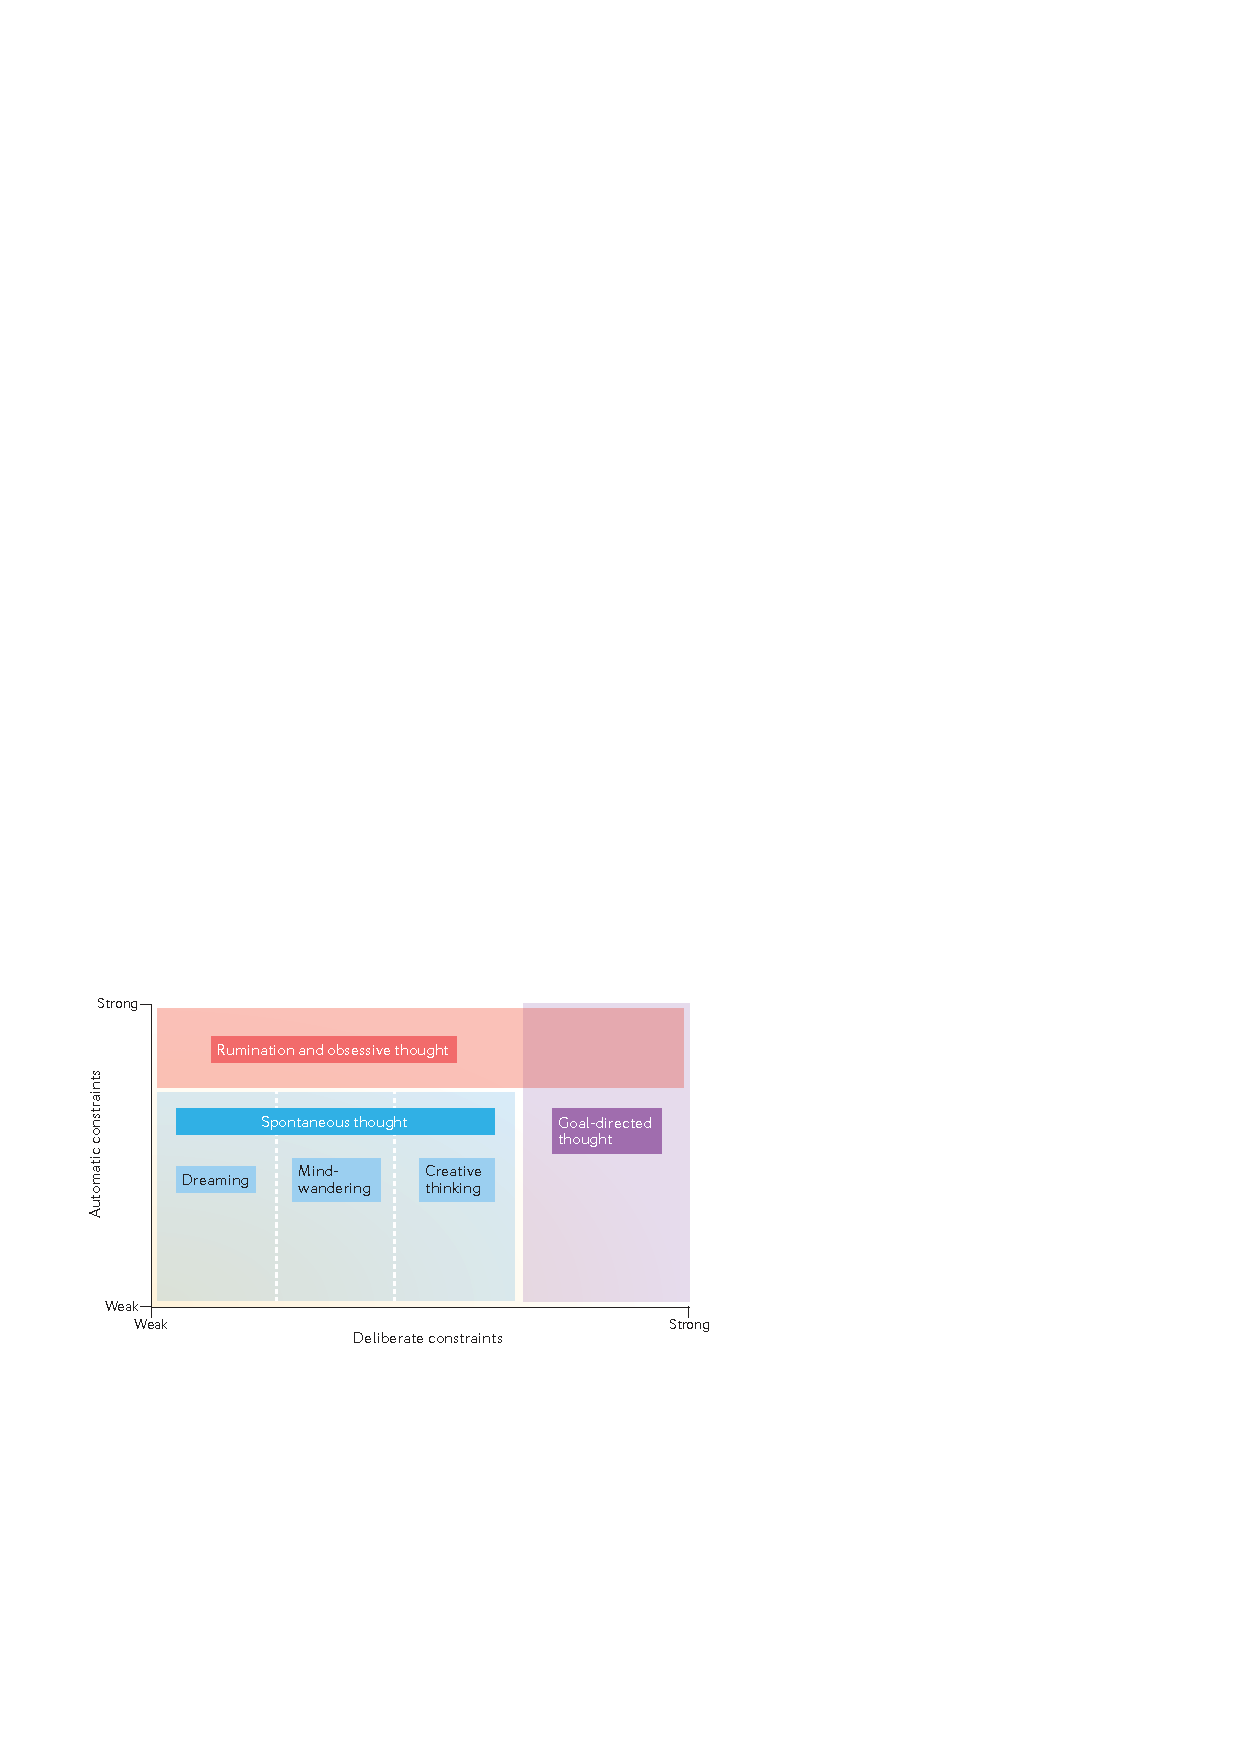
\includegraphics[width=0.75\linewidth]{assets/conceptual_space} 

}

\caption{Conceptual space of different types of thought according to deliberate and automatic constraints (Figure from Christoff et al., 2016).}\label{fig:conceptual}
\end{figure}

Accordingly, cognitive theories of rumination have tried to describe the cognitive mechanisms that are associated with rumination and its perseverative nature. These approaches try to answer questions such as: What are the cognitive underpinnings of the tendency to ruminate? What kind of cognitive biases does rumination cause? To answer these questions, the cognitive control processes that are the most often investigated in relation to depression (and rumination) are the ability of i) inhibiting irrelevant content or a prepotent answer, ii) shifting between tasks and iii) updating current working memory content (for reviews, see Mor \& Daches, \protect\hyperlink{ref-mor_ruminative_2015}{2015}; Grahek, Everaert, Krebs, \& Koster, \protect\hyperlink{ref-grahek_cognitive_2018}{2018}; LeMoult \& Gotlib, \protect\hyperlink{ref-lemoult_depression_2019}{2019}). Linville (\protect\hyperlink{ref-linville_attention_1996}{1996}) first suggested that deficits in attention inhibition may underlie rumination. This proposition was later confirmed and refined by Joorman and colleagues (e.g., Joormann \& Gotlib, \protect\hyperlink{ref-joormann_emotion_2010}{2010}; Joormann \& Vanderlind, \protect\hyperlink{ref-joormann_emotion_2014}{2014}; Joormann, Yoon, \& Zetsche, \protect\hyperlink{ref-joormann_cognitive_2007}{2007}), who shown that rumination is associated with biases in multiple inhibitory processes. They shown that rumination is associated with inhibition deficits with mood-congruent (i.e., negative) material. More precisely, it is proposed that rumination is associated with a decreased ability to limit the access of irrelevant negative information (inhibition) and to discard negative irrelevant information (updating). Koster et al. (\protect\hyperlink{ref-Koster2011}{2011}) proposed that rumination would be the result of a combination of impaired conflict signalling and impaired attentional control. A conflict usually emerges when self-evaluative negative thinking is cued by internal or external stressors and conflicts with an individual's goals. According to this model, it is an impaired conflict signalling \emph{and} an impaired ability to \emph{disengage} attention from self-relevant negative information that explains prolonged ruminative thinking. This idea has been since corroborated by experimental work showing that difficulty disengaging attention was associated with rumination (e.g., Grafton, Southworth, Watkins, \& MacLeod, \protect\hyperlink{ref-grafton_stuck_2016}{2016}; Southworth, Grafton, MacLeod, \& Watkins, \protect\hyperlink{ref-southworth_heightened_2017}{2017}) and by a recent meta-analysis (Zetsche, Bürkner, \& Schulze, \protect\hyperlink{ref-zetsche_shedding_2018}{2018}).

Another view on the relation between cognitive control and rumination has been developed by Whitmer \& Gotlib (\protect\hyperlink{ref-Whitmer2013}{2013}) and is known as the attentional scope model of rumination. In this framework, negative mood would \enquote{facilitate} rumination by narrowing the scope of attention. A narrowed scope of attention would limit the the number of available thoughts and reduce the ability to inhibit irrelevant information or to switch to other information. In contrast, a broader attentional scope (e.g., caused by positive mood) would increase the array of available thoughts. Although some studies indeed found a narrower attentional breadth following a rumination induction (e.g., Grol, Hertel, Koster, \& De Raedt, \protect\hyperlink{ref-grol_effects_2015}{2015}), it is not clear whether attentional breadth is causally involved in ruminative thinking. For instance, Fang et al. (\protect\hyperlink{ref-fang_can_2017}{2017}) failed to obtain transfer effects following a visual attentional breadth training.

Overall, a large number of studies has demonstrated that cognitive control abilities are impaired in individuals with a strong propensity to ruminate (trait rumination) or following a rumination induction (state rumination). For instance, Davis \& Nolen-Hoeksema (\protect\hyperlink{ref-Davis2000}{2000}) showed that ruminators (in comparison with non-ruminators) committed more errors in the Wisconsin card sorting task, highlighting a lack of cognitive flexibility in ruminators. Another study using a mixed antisaccade task showed an impaired inhibition but intact switching abilities in ruminators (De Lissnyder, Derakshan, De Raedt, \& Koster, \protect\hyperlink{ref-DeLissnyder2011}{2011}). Using the Stroop task, Philippot \& Brutoux (\protect\hyperlink{ref-Philippot2008}{2008}) observed that rumination was associated with impaired inhibition. Moreover, recent results suggest that training inhibition might reduce the negativity bias and state rumination (e.g., Daches \& Mor, \protect\hyperlink{ref-daches_training_2014}{2014}; Daches, Mor, \& Hertel, \protect\hyperlink{ref-daches_training_2019}{2019}). Experimental work also demonstrated that difficulties in shifting between different tasks was associated with higher levels of rumination (particularly brooding) in both depressed and nonclinical participants (for reviews, see Koster, Hoorelbeke, Onraedt, Owens, \& Derakshan, \protect\hyperlink{ref-koster_cognitive_2017}{2017}; LeMoult \& Gotlib, \protect\hyperlink{ref-lemoult_depression_2019}{2019}; Mor \& Daches, \protect\hyperlink{ref-mor_ruminative_2015}{2015}; Whitmer \& Gotlib, \protect\hyperlink{ref-Whitmer2013}{2013}).

Studies using cognitive bias modification also permit to experimentally manipulate information-processing biases to assess their effect on mood and behaviour. For instance, Siegle, Ghinassi, \& Thase (\protect\hyperlink{ref-siegle_neurobehavioral_2007}{2007}) showed that participants who received six sessions of cognitive control training (the attention control training and the paced auditory serial attention task, Wells, \protect\hyperlink{ref-wells_emotional_2000}{2000}; Gronwall, \protect\hyperlink{ref-gronwall_paced_1977}{1977}) presented reduced levels of rumination after the training. Hoorelbeke \& Koster (\protect\hyperlink{ref-hoorelbeke_internet-delivered_2017}{2017}) confirmed this finding by showing that an internet-delivered training of ten sessions lead to reduced levels of rumination and depressive symptoms after the training in remitted depressed patients (for a review of cognitive control interventions for depression, see Koster et al., \protect\hyperlink{ref-koster_cognitive_2017}{2017}).

In brief and as summarised by van Vugt, van der Velde, \& ESM-MERGE Investigators (\protect\hyperlink{ref-van_vugt_how_2018}{2018}), the cognitive approaches of rumination can be said to be divided into three (non-exclusive) classes. These approaches consider rumination i) as arising from a bias toward negatively valenced information (e.g., Whitmer \& Gotlib, \protect\hyperlink{ref-Whitmer2013}{2013}), ii) as arising from difficulties in discarding or disengaging from negative and self-relevant information (e.g., Koster et al., \protect\hyperlink{ref-Koster2011}{2011}; Joormann \& Vanderlind, \protect\hyperlink{ref-joormann_emotion_2014}{2014}), or iii) as a \enquote{habit of thoughts} defined by specific pattern of memory associations (e.g., Cramer et al., \protect\hyperlink{ref-cramer_major_2016}{2016}). Following the later conception, van Vugt et al. (\protect\hyperlink{ref-van_vugt_how_2018}{2018}) developed a computational model of rumination implementing the idea that rumination can be considered a maladaptive habit of thought. They showed how rumination can result from particular configurations of memory chunks and their associative structure. This model was able to predict the decline in cognitive task performance observed in depressed patients. Therefore, the computational approach in psychopathology and psychiatry might permit to implement the cognitive models described previously and to make testable predictions about cognitive tasks performance (see also Grahek, Shenhav, Musslick, Krebs, \& Koster, \protect\hyperlink{ref-grahek_motivation_2019}{2019}, for a mechanistic approach of motivation and cognitive control in depression).

\hypertarget{measures-of-rumination}{%
\subsection{Measures of rumination}\label{measures-of-rumination}}

In the following, we make a distinction between measures aiming to assess the stable tendency of individuals to engage in rumination (i.e., trait rumination) and measures aiming to assess the presence, quality or intensity of momentary rumination (i.e., state rumination). Likewise, we present and discuss several types of measures, from self-reported measures to physiological measures. For each type of measure, we first present and discuss measures of trait rumination before turning to measures of state rumination.

Rumination has traditionally been assessed through self-administered questionnaires. The most commonly used measure of trait rumination is the ruminative response scale (RRS) of the response style questionnaire (RSQ, Nolen-Hoeksema \& Morrow, \protect\hyperlink{ref-nolen-hoeksema_prospective_1991}{1991}). The RSQ is an operationalisation of rumination as it was conceptualised in the response styles theory (Nolen-Hoeksema, \protect\hyperlink{ref-nolen-hoeksema_responses_1991}{1991}). The RRS consists of 22 items describing responses to dysphoric mood that are self-focused, symptom-focused, and focused on the causes and consequences of one's mood. A short version of the scale containing ten items has been shown to be highly related (r = .90) to the full version of the questionnaire (Nolen-Hoeksema \& Jackson, \protect\hyperlink{ref-nolen-hoeksema_mediators_2001}{2001}). However, it has been argued that the RRS might contain overlapping items between rumination and depression (Treynor et al., \protect\hyperlink{ref-treynor_rumination_2003}{2003}). In response to these concerns, Treynor et al. (\protect\hyperlink{ref-treynor_rumination_2003}{2003}) removed the ambiguous items from the original RRS and conducted a novel factor analysis. This analysis revealed two distinct components: brooding and reflective pondering (as discussed in the previous section).

Based on Watkins (\protect\hyperlink{ref-Watkins2008}{2008})' distinction between constructive (concrete experiential thinking) and unconstructive (abstract analytical thinking) forms of rumination described previously, Barnard, Watkins, Mackintosh, \& Nimmo-Smith (\protect\hyperlink{ref-barnard_getting_2007}{2007}) developed the Cambridge Exeter Repetitive Thought scale (CERTS) to assess different facets of rumination. This questionnaire contains 84 items arranged in three parts assessing i) the context of rumination, ii) the self-evaluation of the functionality of rumination and iii) ruminative processes. The short version of this questionnaire, the Mini-CERTS (Douilliez, Philippot, Heeren, Watkins, \& Barnard, \protect\hyperlink{ref-Douilliez2012}{2012}), contains 16 items extracted from the third part of the CERTS. These items evaluate more specifically the two dimensions identified by Watkins (\protect\hyperlink{ref-Watkins2008}{2008}). Interestingly, the concrete dimension of the Mini-CERTS appears to be related to the brooding dimension of the RRS whereas no relation was found between the concrete dimension of the Mini-CERTS and other subscales from the RRS (Douilliez et al., \protect\hyperlink{ref-Douilliez2012}{2012}).

Several questionnaires have also been developed to assess the tendency to ruminate (i.e., trait rumination) as a transdiagnostic process. This includes (amongst others) the rumination-reflection questionnaire (Trapnell \& Campbell, \protect\hyperlink{ref-trapnell_private_1999}{1999}), the repetitive thinking questionnaire (McEvoy, Mahoney, \& Moulds, \protect\hyperlink{ref-McEvoy2010}{2010}) or the perseverative thinking questionnaire (Ehring et al., \protect\hyperlink{ref-Ehring2011}{2011}). Several other measures have also been developed to assess more specific forms of repetitive thoughts or processes related to ruminative thoughts such as meta-cognitions, thought control or stress or sadness-reactive rumination (for a review of existing measures of rumination, see Luminet, \protect\hyperlink{ref-luminet_assessment_2004}{2004}).

Rumination can also be seen as a momentary response (state rumination). The effects of state rumination are usually assessed in laboratory settings where rumination is induced and compared to another (more adaptive) form of emotion regulation such as distraction or problem-solving (for review, see Lyubomirsky, Layous, Chancellor, \& Nelson, \protect\hyperlink{ref-lyubomirsky_thinking_2015}{2015}). Some measures have been developed to assess state rumination but usually in reaction to specific events (e.g., stress-reactive, offence-reactive or sadness-reactive rumination). Moreover, until recently, there was no comprehensive and validated measure of state rumination. Nevertheless, the increasing use of the experience sampling methodology (Csikszentmihalyi \& Larson, \protect\hyperlink{ref-csikszentmihalyi_validity_1987}{1987}) to investigate rumination in a more naturalistic environment lead to the development of short scales that could be used quickly and repetitively throughout the day. For instance, Moberly \& Watkins (\protect\hyperlink{ref-Moberly2008}{2008}) operationnalised momentary ruminative thinking using two items. The first item asked participants to rate the extent to which they were focused on their symptoms, consistent with the conceptualisation of rumination of the response styles theory (Nolen-Hoeksema, \protect\hyperlink{ref-nolen-hoeksema_responses_1991}{1991}). The second item asked participants to rate the extent to which they were focused on their problems, consistent with self-regulation theories (Carver \& Scheier, \protect\hyperlink{ref-carver_self-regulation_1998}{1998}; Martin \& Tesser, \protect\hyperlink{ref-Martin}{1996}). Moberly \& Watkins (\protect\hyperlink{ref-Moberly2008}{2008}) considered this two-item measure to reflect \enquote{ruminative self-focus}, independently of current (negative) affects. These two items are rated on a scale from 0 (not at all) to 7 (very much), from which a mean score is then computed.\footnote{The exact items are not specified in Moberly \& Watkins (\protect\hyperlink{ref-Moberly2008}{2008}). However, Huffziger, Ebner-Priemer, Koudela, Reinhard, \& Kuehner (\protect\hyperlink{ref-Huffziger2012}{2012}) used a similar methodology and report the items they used, which were \enquote{At the moment, I am thinking about my feelings} and \enquote{At the moment, I am thinking about my problems}.}

Very recently, Marchetti, Mor, Chiorri, \& Koster (\protect\hyperlink{ref-marchetti_brief_2018}{2018}) developed the brief state rumination inventory (BSRI) to provide a more comprehensive and validated measure of state rumination. They report two studies showing good reliability and validity of this scale in both its English and Dutch version. This questionnaire is composed of eight visual analogue scales (VAS) ranging from \enquote{completely disagree} (numerically recoded as 0) to \enquote{totally agree} (numerically recoded as 100). These items are then summed to provide an indicator of momentary rumination. The BSRI is (to the best of our knowledge) the first validated full-length scale assessing momentary rumination.

Overall, the validity of self-report measures is based on the hypothesis that individuals have a reliable access to their internal states. However, we know self-reports increase reconstruction biases (e.g., Brewer, \protect\hyperlink{ref-rubin_what_1986}{1986}; Conway, \protect\hyperlink{ref-conway_autobiographical_1990}{1990}). Moreover, we know that individuals usually have a low level of awareness of the cognitive processes that underlie their behaviours (Nisbett \& Wilson, \protect\hyperlink{ref-nisbett_telling_1977}{1977}). To overcome these difficulties, some authors have attempted to quantify state rumination and trait rumination more objectively, by recording physiological or neuroanatomical correlates of rumination (for a review, see Siegle \& Thayer, \protect\hyperlink{ref-papageorgiou_physiological_2003}{2003}). Peripheral physiological manifestations (e.g., pupil dilation, blood pressure, cardiac rhythm, cardiac variability) have been examined during induced rumination or in association with trait rumination. For instance, a consistent link between perseverative cognition and decreased HRV was also found in a meta-analysis conducted by Ottaviani et al. (\protect\hyperlink{ref-ottaviani_physiological_2016}{2016}). They also observed a positive association between (both trait and state) perseverative cognition and increased heart rate, systolic blood pressure, diastolic blood pressure, and cortisol activity (see also Zoccola \& Dickerson, \protect\hyperlink{ref-zoccola_assessing_2012}{2012}, for a review of the relation between rumination and cortisol).

With regards to state rumination, Vickers \& Vogeltanz-Holm (\protect\hyperlink{ref-vickers_effects_2003}{2003}) have observed an increased systolic blood pressure after rumination induction, suggesting the involvement of the autonomic nervous system in rumination. Moreover, galvanic skin response has shown to be increased after a rumination induction in highly anxious women (Sigmon, Dorhofer, Rohan, \& Boulard, \protect\hyperlink{ref-sigmon_impact_2000}{2000}). According to Siegle \& Thayer (\protect\hyperlink{ref-papageorgiou_physiological_2003}{2003}), disrupted autonomic activity could provide a reliable physiological correlate of rumination. In this vein, Key, Campbell, Bacon, \& Gerin (\protect\hyperlink{ref-Key2008}{2008}) have observed a diminution of the high-frequency component of heart rate variability (HF-HRV) after rumination induction in people with a low tendency to ruminate (see also Woody, McGeary, \& Gibb, \protect\hyperlink{ref-woody_brooding_2014}{2014}). Moreover, Zoccola, Rabideau, Figueroa, \& Woody (\protect\hyperlink{ref-zoccola_cardiovascular_2014}{2014}) showed that the physiological consequences of rumination might depend on the level of construal (i.e., abstract vs.~concrete). More precisely, they showed that an induction of abstract rumination lead to lower blood pressure in comparison an induction of concrete rumination. Woody, Smolak, Rabideau, Figueroa, \& Zoccola (\protect\hyperlink{ref-woody_trait_2015}{2015}) further showed that the type of ruminative thought (imagery vs.~verbal thought) was also associated with distinct physiological outcomes. They observed that verbal ruminative thoughts lead to greater increases in heart rate than ruminative thoughts in a visual imagery modality. This effect was moderated by trait rumination and was only present in high ruminators.

In the present work, we used facial surface electromyography (in addition to self-reports) to investigate the muscular correlates of induced rumination. Before turning to a presentation of this experimental work however, we need to discuss why we think rumination can be considered a form of inner speech and how inner speech (and therefore, by inclusion, rumination) can be examined using surface electromyography.

\hypertarget{on-the-verbal-and-sensory-properties-of-rumination}{%
\subsection{On the verbal and sensory properties of rumination}\label{on-the-verbal-and-sensory-properties-of-rumination}}

One of the most salient features of rumination is that it is mostly expressed in a verbal modality (Ehring \& Watkins, \protect\hyperlink{ref-ehring_repetitive_2008}{2008}; Goldwin \& Behar, \protect\hyperlink{ref-goldwin_concreteness_2012}{2012}; Goldwin, Behar, \& Sibrava, \protect\hyperlink{ref-goldwin_concreteness_2013}{2013}; McLaughlin, Borkovec, \& Sibrava, \protect\hyperlink{ref-mclaughlin_effects_2007}{2007}). In other words, while ruminating, we are mostly talking to ourselves silently. However, rumination can also be experienced as visual imagery (Goldwin \& Behar, \protect\hyperlink{ref-goldwin_concreteness_2012}{2012}; Newby \& Moulds, \protect\hyperlink{ref-newby_comparison_2012}{2012}; Pearson, Brewin, Rhodes, \& McCarron, \protect\hyperlink{ref-pearson_frequency_2008}{2008}). By \enquote{visual imagery} we refer to a process during which perceptual information is retrieved from long-term memory, resulting in the experience of \enquote{seeing with the mind's eye} (Ganis, Thompson, \& Kosslyn, \protect\hyperlink{ref-ganis_brain_2004}{2004}). Some authors have suggested that because rumination is usually past-oriented, it should increase access to negative autobiographical memories (Lyubomirsky et al., \protect\hyperlink{ref-Lyubomirsky1998}{1998}). Moreover, because autobiographical memories are often experienced as visual images, rumination should likewise include visual features (Pearson et al., \protect\hyperlink{ref-pearson_frequency_2008}{2008}). Several studies have obtained results that are consistent with this claim. Among a sample of patients who were diagnosed as clinically depressed, a significant majority (94.7\% and more than 70\%) reported that rumination combined verbal and sensory elements, among which visual imagery (Newby \& Moulds, \protect\hyperlink{ref-newby_comparison_2012}{2012}; Pearson et al., \protect\hyperlink{ref-pearson_frequency_2008}{2008}, respectively). When unselected individuals were asked about the quality of their rumination directly while ruminating, 60.53\% of them said they had been experiencing verbal thoughts and 35.92\% mental visual images (McLaughlin et al., \protect\hyperlink{ref-mclaughlin_effects_2007}{2007}). Another study comparing naturally occurring depressive and anxious thoughts in a non-clinical sample, found that depressive thoughts involved more images than anxious thoughts (Papageorgiou \& Wells, \protect\hyperlink{ref-papageorgiou_process_1999}{1999}). In addition, a recent study demonstrated that a considerable number of people experience depressive cognition in a visual form (Lawrence, Haigh, Siegle, \& Schwartz-Mette, \protect\hyperlink{ref-lawrence_visual_2018}{2018}). Furthermore, this study showed that individuals with a visual depressive cognitive style reported a similar amount of rumination as individuals with a verbal style. Overall, the existing literature indicates that rumination can have visual features, despite being predominantly verbal.

These observations about the quality of ruminative thoughts are consistent with those concerning worry (e.g., Stöber, \protect\hyperlink{ref-stober_worry_1998}{1998}; McLaughlin et al., \protect\hyperlink{ref-mclaughlin_effects_2007}{2007}). Indeed the cognitive avoidance theory (Sibrava \& Borkovec, \protect\hyperlink{ref-davey_cognitive_2006}{2006}) suggest that worry, as a primarily linguistic repetitive thought, can be considered an avoidance response whose goal is to restrain aversive images, thus reducing somatic activation and emotion processing. Similarly, forming negative mental visual images has been shown to lead to a greater increase in anxiety in comparison to forming negative descriptive sentences (Holmes \& Mathews, \protect\hyperlink{ref-holmes_mental_2005}{2005}). Taken together, these findings suggest that different modalities of rumination could have different effects on individuals. This idea is supported by studies showing the effectiveness of mental imagery in accessing and modifying emotion in therapy (for an overview, see Hackmann \& Holmes, \protect\hyperlink{ref-hackmann_reflecting_2004}{2004}). Overall, investigating the verbal and visual features of rumination could contribute to sharpen our understanding of the ruminative processes and lead to better-adapted therapeutic strategies.

Some of the few studies specifically manipulating verbal and visual rumination were carried out by Zoccola and colleagues (Woody et al., \protect\hyperlink{ref-woody_trait_2015}{2015}; Zoccola et al., \protect\hyperlink{ref-zoccola_cardiovascular_2014}{2014}). The verbal or visual form of rumination (or \emph{mentation type} as these authors refer to it) was induced by playing audio tapes that directed participants' thoughts. Prompts were similar in both conditions, differing only in the verbal/visual instruction (\enquote{Recall the speech task using words, phrases, and sentences.} vs.~\enquote{Recall the speech task using pictures and images.}). Participants were subsequently asked to estimate the proportion of verbal thoughts and mental visual images. Importantly, it should be noted that in none of the studies in which thinking modality was manipulated, did the participants solely use one type of thought. Even though participants in the imagery group of Zoccola et al. (\protect\hyperlink{ref-zoccola_cardiovascular_2014}{2014}) reported higher levels of mental images in comparison to the participants in the verbal group, the later group also reported a certain level of mental imagery. This is in line with studies showing that rumination includes both verbal and visual components (e.g., Goldwin \& Behar, \protect\hyperlink{ref-goldwin_concreteness_2012}{2012}; McLaughlin et al., \protect\hyperlink{ref-mclaughlin_effects_2007}{2007}), implying that it is not exclusively experienced in one modality. These results are substantiated by a recent study which has shown that participants generate visual images both in cases where they were told to visualise or to verbally think, while they have strong verbal representations only when asked to verbally think (Amit, Hoeflin, Hamzah, \& Fedorenko, \protect\hyperlink{ref-amit_asymmetrical_2017}{2017}). Amit et al. (\protect\hyperlink{ref-amit_asymmetrical_2017}{2017}) concluded that there is a difference in volitional control of verbal and visual thinking and that people have better control over inner speech than visual thought.

To sum up, although rumination might be expressed in different modalities, it is usually expressed in a verbal form. Therefore, we suggest that \emph{verbal} rumination migh be considered as a form of inner speech. To understand what this assumption implies for the study of rumination, we now turn to a brief historical overview of inner speech research. This historical tour will allow us to introduce the experimental tools that have been used to investigate inner speech throughout history. We will then present the main theoretical perspectives on inner speech and discuss its analogies with the broader phenomenon of motor imagery.

\hypertarget{what-is-that-little-voice-inside-my-head}{%
\section{What is that little voice inside my head?}\label{what-is-that-little-voice-inside-my-head}}

To begin our investigation with a clear definition, when we use the term of \enquote{inner speech}, we refer broadly to the activity of silently talking to oneself. Whereas the exact nature of inner speech is still the matter of lively debates, Gregory (\protect\hyperlink{ref-gregory_inner_2017}{2017}) lists some consensual properties of inner speech, namely, that i) inner speech takes place in the mind, ii) an instance of inner speech is a linguistic occurrence, iii) inner speech is episodic (i.e., it occurs at a given moment in time), iv) an episode of inner speech involves mental imagery (may it be auditory, visual, or kinaesthetic imagery), v) inner speech can be used in the service of working memory, vi) inner speech does not \emph{necessarily} (and often does not) take the form of complete grammatical sentences (cf.~our later discussion of Vygotsky's theory of inner speech development), vii) we do not have the same level of control upon our inner speech than upon our overt speech (whereas it is easy to stop producing external speech, it can be quite arduous to override inner speech).

Whereas we produce inner speech on a daily basis to conduct inner monologues or dialogues, to prepare or to remember conversations, this activity remains nevertheless arduous to investigate in a controlled environment. Like most psychological phenomena, the study of inner speech started with introspective observations (Morin, \protect\hyperlink{ref-morin_inner_2009}{2009}). At the end of the XIXth century and throughout the XXth century, experimental psychologists gave a new look at inner speech through novel (neuro)physiological methods (we review these findings later on). As a result of being both a multi-facetted phenomenon (inner speech can be expressed in many forms or \emph{varieties}) and being studied from different perspectives (from philosophy to linguistics and neurosciences), the activity of inner speech has been given many other names such as covert speech, subvocal speech, verbal thinking, implicit speech, internal monologue, internal dialogue, endophasy, speech imagery, auditory verbal imagery, silent talk or silent speech. This plethora of names might be explained by the variety of the activity in itself but also by the relatively vague definition that is usually attached to it.

Indeed, as noted by Vygotsky (\protect\hyperlink{ref-vygotsky_thought_2012}{2012}), the term of inner speech has been used to describe somehow different phenomena. More precisely, Vygotsky (\protect\hyperlink{ref-vygotsky_thought_2012}{2012}) suggested that this term has initially been employed to refer to \enquote{verbal memory}, citing for example the \enquote{silent recital of a peom known by heart} (p.238). In that vein, Cardaillac (\protect\hyperlink{ref-cardaillac_etudes_1830}{1830}) earlier said: \enquote{la parole intérieure n'est que le souvenir de la sensation que produit la parole extérieure} (as quoted in Egger, \protect\hyperlink{ref-egger_parole_1881}{1881}, p. 53).\footnote{Which can be translated by \enquote{inner speech is only the memory of the sensation produced by external speech}.} Accordingly, investigations of inner speech conducted throughout the XIXth century mostly revolved around the question of finding how words were reproduced in memory (either as auditory, visual or motor images). Under that view, inner speech is thought to correspond to an \enquote{image} of actual (overt) speech and this position may be said to correspond to the \emph{imagined speech view} described in Gregory (\protect\hyperlink{ref-gregory_inner_2017}{2017}).

According to the second perspective listed by Vygotsky (\protect\hyperlink{ref-vygotsky_thought_2012}{2012}), inner speech could be conceived as truncated overt speech, that is, \enquote{speech minus sounds} or \enquote{subvocal speech} (Watson, \protect\hyperlink{ref-watson_psychology_1919}{1919}). For instance, in line with his reflexologist theory of thought, Sechenov considered inner speech to be an inhibited (motor) reflex and wrote: \enquote{I never think directly in words, but always instead in muscular sensation which accompany my thought in the form of a conversation} (cited in Sokolov, \protect\hyperlink{ref-sokolov_inner_1972}{1972}, p. 4). It should be noted however, as highlighted by Sokolov (\protect\hyperlink{ref-sokolov_inner_1972}{1972}), that the behaviourist approach and the reflex approach differ in that the former consider that inner speech \enquote{originate} from peripheral muscular activations, whereas the later consider inner speech to result from central (cerebral) processes. According to that latter perspective, the peripheral muscular activity recorded during imagined actions (or inner speech) would be a side-effect of these central processes.\footnote{We will comme back to this important distinction in more details later under the disguise of the \enquote{centralism versus peripheralism} debate.} In that view, inner speech is considered as an actual speech (as overt speech is) and not to correspond to an \enquote{image} of overt speech. This position may be said to correspond to the \emph{actual speech view} described in Gregory (\protect\hyperlink{ref-gregory_inner_2017}{2017}).

According to Vygotsky (\protect\hyperlink{ref-vygotsky_thought_2012}{2012}), a third interpretation of inner speech would refer to everything that \enquote{precedes the motor act of speaking}. In other words, inner speech would include speech \enquote{motives} (or intentions) and the preverbal message that precedes speech production. We will come back to that position briefly when mentioning psycholinguistic models of speech production (e.g., Levelt, \protect\hyperlink{ref-levelt_speaking_1989}{1989}) as well as the motor simulation model of motor imagery (e.g., Jeannerod, \protect\hyperlink{ref-jeannerod_motor_2006}{2006}). However, for the purpose of the current section, we are mostly concerned with the first and second position, namely, the view of inner speech as either imagined or actual speech.

In trying to separate these two views, Gregory (\protect\hyperlink{ref-gregory_inner_2017}{2017}) first notes that, phenomenologically, producing inner speech feels like speaking (albeit covertly), and not like imagining speaking. Gregory then lists some further arguments in favour of the actual speech view: i) \emph{the embedding argument}: we can imagine producing inner speech, but we cannot imagine \emph{imagining} producing inner speech, therefore inner speech is actual speech (rather than imagined speech), ii) \emph{the paralleled case argument}: inner speech stands in the same relation to speech in a pretend scenario as overt speech does, therefore, inner speech is also actual speech (for more details, see Gregory, \protect\hyperlink{ref-gregory_inner_2017}{2017}, p. 40), iii) \emph{the continuity argument}: inner speech sits on a continuum with various kinds of external (and therefore actual) speech, iv) \emph{the precisification argument}: the imagined speech view leaves too much details unspecified (e.g., who is speaking? In what context?), which is not the case of the actual speech view.

While we will not directly assess the empirical arguments in favour of either the \emph{imagined speech} or the \emph{actual speech} view of inner speech, we wanted to give the reader a clear definition of what we mean by \enquote{inner speech} and to present the two main conceptions about the nature of inner speech. We think these two conceptions and the arguments that have been advanced in favour or against each view are worthy to keep in mind while reviewing the empirical evidence on the topic. In the next section, we will briefly review the historical development of ideas and methods used to describe inner speech, before turning to a description of the developmental mechanisms of inner speech and to contemporary neurocognitive models of inner speech production.

\hypertarget{inner-speech-history}{%
\subsection{Historical overview of inner speech investigations}\label{inner-speech-history}}

\hypertarget{from-introspection-to-experimental-psychology}{%
\subsubsection{From introspection to experimental psychology}\label{from-introspection-to-experimental-psychology}}

The question of the relation and intertwinement of thought and language is one of the most enduring philosophical question. Most notable reflections can be traced back to Plato's \emph{Theaetetus}, in which Plato defines thinking as \enquote{the conversation which the soul holds with itself in considering anything}. For Plato, the definition of thinking is taken to correspond to \enquote{word{[}s{]} spoken in silence}. Sokolov (\protect\hyperlink{ref-sokolov_inner_1972}{1972}) notes that ancient thinkers, by noticing a relation between thoughts and words, and between words and breathing, used to think that thoughts and words originated in the lungs. For instance, Socrates, in Plato's \emph{Phaedrus}, said that \enquote{his chest is full of thoughts} (as quoted in Sokolov, \protect\hyperlink{ref-sokolov_inner_1972}{1972}, p. 14). In another context, by noting the progressive internalisation of external speech into inner speech during normal development, Egger (\protect\hyperlink{ref-egger_parole_1881}{1881}) wonders whether the phylogeny (the evolution of the species) followed this same course of development. In support of that idea, Egger (\protect\hyperlink{ref-egger_parole_1881}{1881}) reports the existence of an ancient Egyptian ideogram, representing a crouched man, with the right hand close to the mouth. Egger (\protect\hyperlink{ref-egger_parole_1881}{1881}) explains that this ideogram was meant to represent undistinctly the ideas of eating, drinking, screaming, talking, meditating, knowing or judging, suggesting that thought was considered to be localised in the mouth (p.84).

Somehow consistently with that idea, Stricker (\protect\hyperlink{ref-stricker_studien_1880}{1880}) reported (based on his own introspections) that he was not able to mentally produce speech sounds without making movements with the articulators. He also reported not being able to produce two different speech sounds, or to produce speech sounds that were incongruent with movement of the articulators. To give a reproducible example of his intuition, Stricker (\protect\hyperlink{ref-stricker_studien_1880}{1880}) suggested the following experiment: open your mouth and try to pronounce a word including labials or dentals, such as \enquote{bubble} or \enquote{toddle}. Ask yourself whether the image of the word (your inner speech) is clear or distinct? According to Stricker, most people would find it very difficult to imagine cleary these words with the mouth being open. Instead, the image of the work is rather imprecise and sounds like we were trying to produce (overtly) the word while keeping the mouth open. This sensation was already nicely described and analysed by Bain (\protect\hyperlink{ref-bain_senses_1855}{1855}):

\begin{quote}
\enquote{When we recall the impression of a word or sentence, if we do not speak it out, we feel the twitter of the organs just about to come to that point. The articulating parts --the larynx, the tongue, the lips,-- are all sensibly excited; a suppressed articulation is in fact the material of our recollection, the intellectual manifestation, the idea of speech.}
\end{quote}

James (\protect\hyperlink{ref-james_principles_1890}{1890}) then notes that Stricker, \enquote{Like most psychologists, however, {[}\ldots{]} makes of his personal peculiarities a rule, and says that verbal thinking is normally and universally an exclusively motor representation.} Indeed, Paulhan (\protect\hyperlink{ref-paulhan_langage_1886}{1886}) replied to Stricker that he was able to produce overtly the phoneme /a/ while simultaneously being able to get and maintain the mental image of any other vowel. He also reported that he was able to imagine the sound of any vowel without motor actions or feelings (images). On a similar note, Egger (\protect\hyperlink{ref-egger_parole_1881}{1881}) believed inner speech to exist independently of motor phenomena and to be based predominantly on auditory representations. He noticed that although inner speech may be accompanied by vivid auditory imagery, inner speech is also very different from overt (external) speech, with inner speech being usually shorter and less grammatically structured than overt speech (we will come back to that observation later when discussing the development of inner speech).

In an attempt to reconcile the view of Stricker (\protect\hyperlink{ref-stricker_studien_1880}{1880}) for whom inner speech was purely motor with the view of Paulhan (\protect\hyperlink{ref-paulhan_langage_1886}{1886}) and Egger (\protect\hyperlink{ref-egger_parole_1881}{1881}), Ballet (\protect\hyperlink{ref-ballet_langage_1886}{1886}) suggested (as James, \protect\hyperlink{ref-james_principles_1890}{1890}), that these authors probably generalised to the population what they observed on themselves. Ballet then asserted that the predominance of motor over sensory representations (or the reverse) might be a question of individual differences. We might add that the relative predominance of motor or sensory representations during inner speech might also be due to individual differences in the phenomenological sensitivity to some specific representation (some might be very acute in discriminating similar auditory images while not being able to discriminate similar visual images) and to contextual differences.\footnote{Indeed, it is plausible that the predominance of some sort of representation over other forms might be contingent on contextual demands. In other words, depending on the task to be realised, the motoric and sensory aspects of inner speech might be weighted differently.} Nonetheless, for many authors, this debate highlighted the limitations of the introspective method (e.g., Reed, \protect\hyperlink{ref-reed_existence_1916}{1916}). To be able to decide between different individual experiences and interpretations, some researchers therefore tried to find more objective methods to assess inner speech, or as put by Reed (\protect\hyperlink{ref-reed_existence_1916}{1916}), to go beyond introspection and to start looking for \enquote{the stamp of objective certainty}. With this ambitious goal in mind, Reed (\protect\hyperlink{ref-reed_existence_1916}{1916}) describes an apparatus he used to examine tongue movements (see Figure \ref{fig:reed}). Reed then reports the results of an experiment aiming to examine the involvement of inner speech (and speech motor processes) in thinking.

\begin{figure}

{\centering 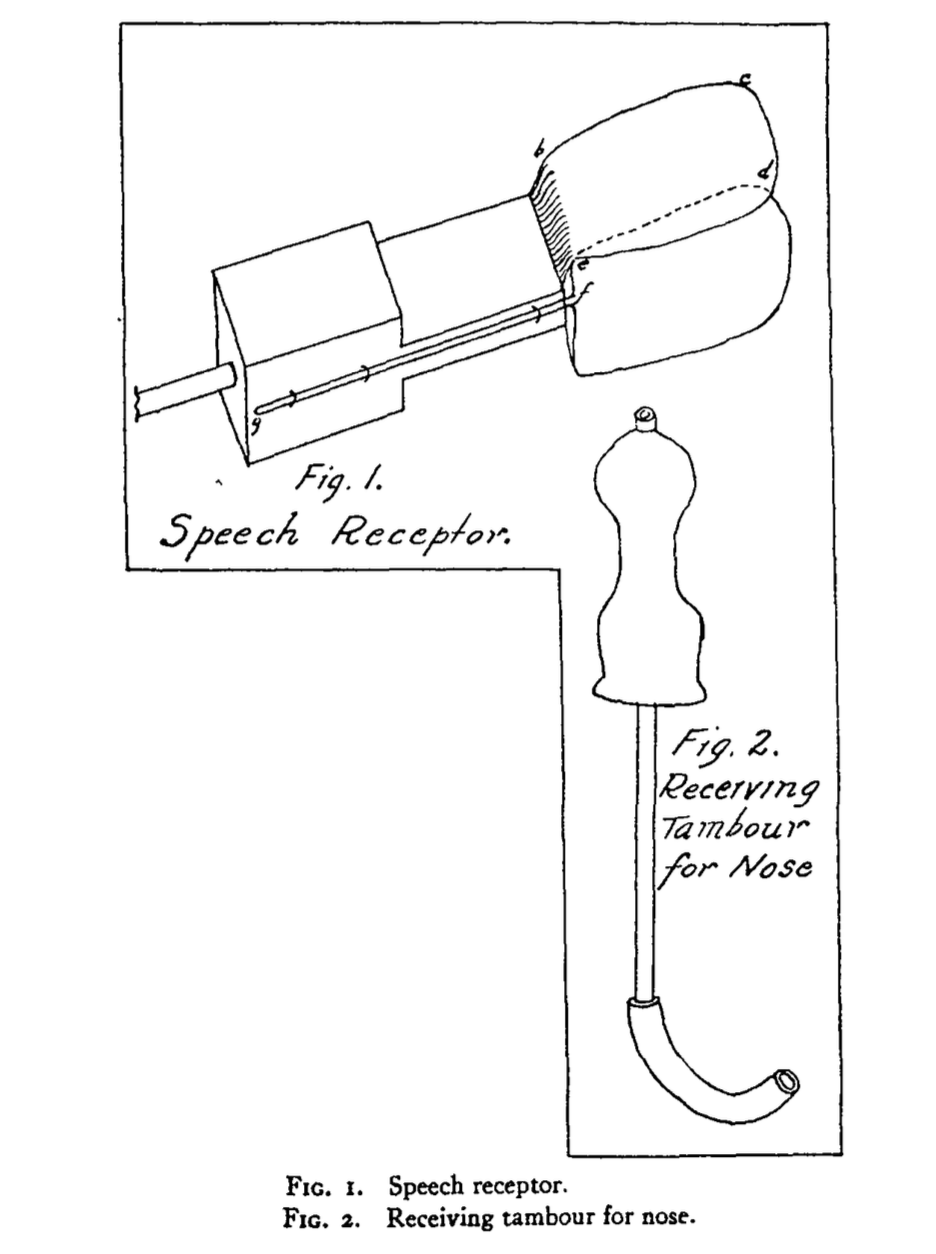
\includegraphics[width=0.5\linewidth]{assets/reed} 

}

\caption{Figure 1 \& 2 from Reed (1916) describing the apparatus used to record tongue movements during thinking and inner speech.}\label{fig:reed}
\end{figure}

Reed (\protect\hyperlink{ref-reed_existence_1916}{1916}) observed that while reading, his participants were moving their tongue and lips (and were sometimes whispering). These observations, in addition to the behaviourist revolution in Psychology paved the way for new lines of research. The initial suggestion of Watson (\protect\hyperlink{ref-watson_psychology_1913}{1913}) that \enquote{thought processes are really motor habits in the larynx} lead to a fruitful line of research about the muscular bases and/or correlates of thought and inner speech. Sokolov (\protect\hyperlink{ref-sokolov_inner_1972}{1972}) gives an overview of the experiments carried out at the beginning of the XXth century in that perspective. For instance, Dodge (\protect\hyperlink{ref-dodge_motorischen_1896}{1896}) anesthetised his lips and tongue and realised that it did not have any impact on his inner speech. Curtis (\protect\hyperlink{ref-curtis_automatic_1900}{1900}) and Courten (\protect\hyperlink{ref-courten_involuntary_1902}{1902}) recorded laryngeal movements using a pneumatic drum and a kymograph while their participants recited verses or were reading. They observed that laryngeal movements were not always present and depended on what was being read and/or produced, as well as on the \enquote{degree of understanding} of the participant (for further references, see Sokolov, \protect\hyperlink{ref-sokolov_inner_1972}{1972}, pp. 43--45).

Using a galvanometer and electrodes inserted in the tip of the tongue, in the cheek, or under the lip, Jacobson (\protect\hyperlink{ref-jacobson_electrical_1931}{1931}) recorded muscular action potential while participants were asked to produce verbal content covertly (e.g., counting or reciting a poem), but not during relaxation. Interestingly, Jacobson (\protect\hyperlink{ref-jacobson_electrical_1931}{1931}) adds that \enquote{the series of vibrations during the mental activity occur in patterns evidently corresponding with those present during actual speech.} More precisely, the pattern of muscular of activity recorded during inner speech production was similar to the pattern of muscular activity recorded during overt speech production, but of lesser amplitude.

Throughout the present section, we briefly reviewed the history of ideas and methods used to describe inner speech in the second part of the XIXth century and at the beginning of the XXth century. In the next section, we make a brief pause in our historical tour to discuss the developmental trajectory of inner speech. How and when do we (humans) acquire the ability to talk to ourselves silently? Is it even acquired? To answer these questions, we will briefly review Vygotsky's theory of inner speech development and some of its more recent refinements. Moreover, by examining how inner speech develops, we might gain new insights about the characteristics of inner speech in the adult mind.

\hypertarget{development}{%
\subsubsection{Interlude: the development of inner speech}\label{development}}

The developmental course of inner speech was possibly the most investigated issue related to inner speech in the first part of the XXth century. Among many, Watson, Piaget, Luria, Leontiev, and most famously Vygotsky confronted this question. Watson (\protect\hyperlink{ref-watson_psychology_1919}{1919}) suggested that thought was rooted in (overt) speech, with maturation leading from speech to thought (where thought is to be understood as a synonym to inner speech, in Watson's terminology). This hypothesis also applied to reading, with the novice reader reading overtly and progressively shifting to silent reading. For Vygotsky, the study of inner speech in the mature (i.e., adult) brain could only be understood from a developmental perspective. In the last chapter of his book \emph{Thought and Language}, Vygotsky analyses the relationship between thought and word in the mature mind. The central idea of this chapter is stated as follows:

\begin{quote}
\enquote{The relationship between thought and language is not a thing, but a process, a continual movement back and forth from thought to word and from word to thought. Viewed in the light of a psychological analysis, this relation is a process that passes through a series of phases and stages, during which its essential features undergo changes that may be called development in the strict sense. Of course, this is a functional development, not development in the sense of aging; but the path traversed by thinking as a process from thought to word is development nonetheless.}
\end{quote}

Fundamentally, Vygostky believed that language was a psychological tool and that its development during childhood interacts with the development of abstract thinking. Vygotsky observed, as Piaget before him, that the child tends to speak (aloud) to himself while playing. Piaget characterised this form of speech as \enquote{egocentric speech} because in this form of speech, according to Piaget, the child does not try to take the perspective of the listener. Piaget thought this form of speech to disappear at the age of seven or eight. In contrast, Vygotsky thought that the so-called egocentric speech (or private speech) continues but that it becomes more and more internalised, until reaching the status of \enquote{inner} speech. For Vygostky, this internalisation process starts with social speech, that is speech addressed to others. During development, this form of speech evolves to either communicative speech (speech addressed to others) and so-called egocentric speech (speech addressed overtly to oneself). This form of speech appears naturally in children while being faced with a problem to solve, but also in adults faced with difficult problems. This egocentric speech would then became internalised, resulting in what we call inner speech. This lead Vygostky to claim a functional equivalence between egocentric speech and internal speech, the later resulting from a progressive internalisation of the former.

However and importantly, this internalisation process does not \emph{only} entail a movement from the outside to the inside but also entails a transformation of speech, or, as put by Vygotsky, an \enquote{internal reconstruction of an external operation}. Therefore, for Vygostky, it follows that the passage from inner speech to overt speech consists not in simply \enquote{vocalising} inner speech but in \emph{restructuring} inner speech (e.g., retrieving a syntax proper to overt speech, retrieving the phonetic structure, etc). According to Vygotsky (\protect\hyperlink{ref-vygotsky_thought_2012}{2012}), inner speech is described by some essential properties such as: i) \emph{abbreviation}: the phonetic aspect is \enquote{diminished}, reduced: \enquote{In inner speech we do not need to pronounce a word in its entirety. We understand, by virtue of our very intention, what word we wanted to say {[}\ldots{]} Strictly speaking, inner speech is almost wordless}, ii) \emph{predicativeness}, \enquote{Psychologically, inner speech consists of predicates only}; \enquote{the subject of our inner reason is always present in our thought}; it is always implicitly understood, iii) it has a semantic structure of its own: predominance of \emph{sense} over \emph{meaning}\footnote{Referring to Paulhan's distinction between the dictionary \emph{meaning} of a word on one hand, and the individual \emph{sense} of a word which is acquired by usage, on the other hand.}, it is idiomatic, agglutination of semantic units (several words can be \enquote{merged} into a single word), and \emph{infusion of sense} into a word (a word in inner speech becomes \enquote{loaded} with more associations than in conventional use).

Interestingly, Vygotsky rejected both the verbal memory view of inner speech (i.e., inner speech is simply the retrieval of acoustic, optic or motor images of words) and the behaviourist view of inner speech as merely a soundless form of external speech (à la Watson). For Vygotsy, the most determining factors of inner speech are its semantic (psychological) features, as expressed by his famous dictum: \emph{Thought is not expressed in words; it comes into existence through them}.

More recently, Fernyhough (\protect\hyperlink{ref-fernyhough_alien_2004}{2004}) proposed an extension of Vygotsky's three-level model of inner speech development (i.e., external speech, egocentric speech, inner speech) to a four-level model, from external dialogue to private speech, expanded inner speech and condensed inner speech (see Figure \ref{fig:fernyhough}). Fernyhough (\protect\hyperlink{ref-fernyhough_alien_2004}{2004}) notes that this model describe stages in the development of inner speech (during childhood) but also movements \enquote{between the levels at any given point in time}. Indeed, it is possible to \enquote{move} between levels under certain conditions. For instance, in cognitively demanding conditions, we can observe transitions between levels, with condensed inner speech being transformed to expanded inner speech and even dialogic private speech through a process of \enquote{re-expansion}. This idea is supported by many studies showing an progressive externalisation of inner speech under cognitively demanding situations (e.g., Sokolov, \protect\hyperlink{ref-sokolov_inner_1972}{1972}).

\begin{figure}

{\centering 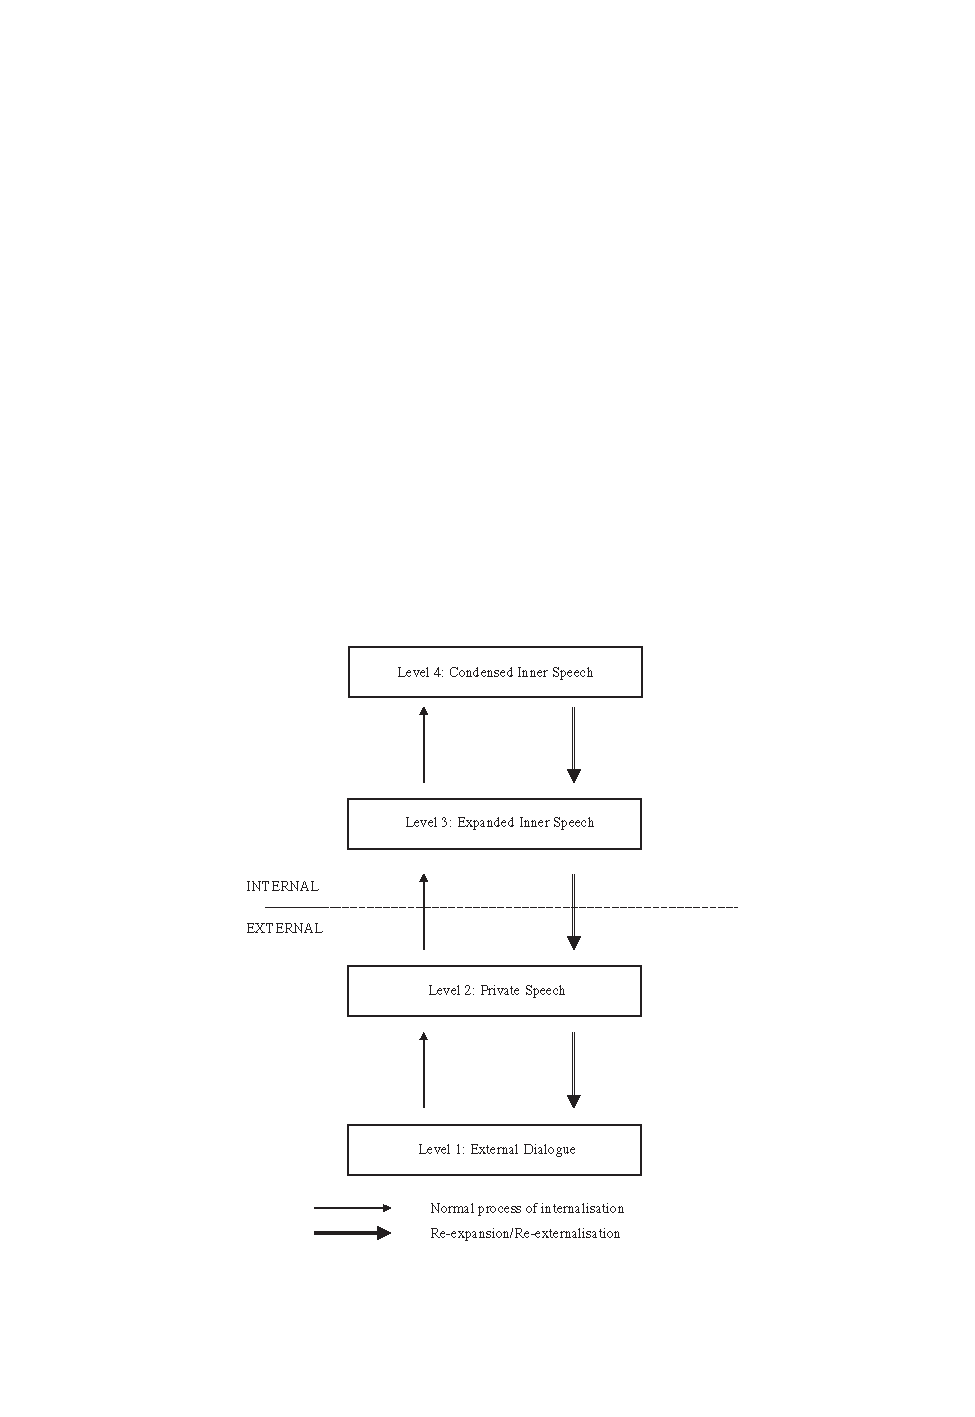
\includegraphics[width=0.75\linewidth]{assets/fernyhough_model_2004} 

}

\caption{Stages of internalisation. Figure from Fernyhough (2004).}\label{fig:fernyhough}
\end{figure}

To sum up, it is suggested that inner speech (in the adult mind) is the result of a progressive internalisation process. This internalisation process covers different stages or expressions of speech from social speech, self-addressed speech (private speech or egocentric speech) to inner speech (first in a very expanded form and then in a more condensed form). Being an internalised version of private speech, inner speech is hypothesised to be attached with the same functions as private speech. In other words, adults use inner speech with the same goals as they previously used (during childhood) overt private speech. Importantly, this internalisation process does not \emph{only} entail an internalisation but also a transformation of the way speech is expressed: the characteristics of inner speech are distinguishable from the characteristics of overt (private) speech. Interestingly, these different levels (or stages) in the internalisation process, in addition to describing stages of development, also describe \enquote{movements} that can be performed between levels or stages. More precisely, the externalisation of inner speech would entail the inverse transformation that has been applied during the internalisation of private speech. In the next section, we come back to our historical perspective by reviewing inner speech research that has been carried out in the second part of the XXth century, before turning to an overview of the main theoretical perspectives about inner speech production.

\hypertarget{inner-speech-research-from-1950-to-present-days}{%
\subsubsection{Inner speech research from 1950 to present days}\label{inner-speech-research-from-1950-to-present-days}}

Following the pioneering work of Jacobson (\protect\hyperlink{ref-jacobson_electrical_1931}{1931}), the second part of the XXth century witnessed an upsurge of electrophysiological methods (and especially of electromyography\footnote{See Chapter \ref{chap2} for a brief introduction to (surface) electromyogaphy.}) to study the production of inner speech. Interestingly, the dominant interpretation of the muscular correlates of inner speech (as identified by Jacobson, \protect\hyperlink{ref-jacobson_electrical_1931}{1931}) at the beginning of the last century was that the peripheral muscular activity observed during imagined actions was the \emph{source} of the mental content. However, as explained by Jeannerod (\protect\hyperlink{ref-jeannerod_motor_2006}{2006}), this interpretation of mental processes as a consequence of peripheral feedback is now disproved, for instance by the simple fact that many people can experiment inner speech (or motor imagery) without any observable muscular activity. From there, one can ask whether the peripheral muscular activity observed during inner speech is \emph{necessary} to the production of inner speech, or rather can be considered a consequence of inner speech production. As pinpointed by Cohen (\protect\hyperlink{ref-cohen_motor_1986}{1986}), to prove that a pattern of motor activity is \emph{necessary} for some mental activity, it is not enough to show that this pattern is always associated with the mental activity, we also have to show that when the pattern of motor activity is disrupted, the mental activity is in turn disrupted. In that vein, the \emph{peripheralist} interpretation of the motor correlates of inner speech (see Box \ref{centralism}) has been disproved by the heroic experiment carried out by Smith, Brown, Toman, \& Goodman (\protect\hyperlink{ref-smith_lack_1947}{1947}). Smith used d-tubocurarine (curare) to paralyse his own facial muscles in order to test whether peripheral muscular activation was necessary to inner speech. He reported that, while being paralysed, he was still able to think in words and to solve mathematical problems (these results echo those of Dodge, \protect\hyperlink{ref-dodge_motorischen_1896}{1896}, mentioned earlier).

Another way of looking at the motor correlates of inner speech production is to assume that these correlates are instead a consequence of central processes involved in inner speech production. As such, a disruption of these correlates do not necessary entail a disruption of the ongoing mental processes. Depending on the framework, these peripheral correlates might be considered as either necessary at the first stages of development of inner speech (as in behaviourist views of inner speech) or not necessary at all in other \emph{centralist} perspectives such as the Russian reflexology or the more recent simulation or emulation frameworks. In these simulationnist frameworks, the peripheral muscular activity observed during inner speech production (or motor imagery) may be hypothesised to be the result of an incomplete inhibition of motor output during the mental states involving motor simulation (although the precise nature of these inhibitory mechanisms is still the matter of debates, cf.~section \ref{motor-imagery}).

\vspace{2mm}

\begin{mybox}[label = centralism]{Centralism versus peripheralism}

Many studies have shown that inner speech and, more generally, imagined actions, may be accompanied by peripheral muscular activation. However, the status of this muscular activity might be interpreted in several ways. According to the \textit{peripheralist view}, the mental image of an object would arise from muscular discharges in the related muscles (cf. work from James, 1890; Jacobson, 1931). In other words, for the tenants of this view, the peripheral muscular activity is a \textit{necessary} condition for the generation of the corresponding mental image.\\

According to the \textit{centralist view}, the existence of a muscle discharge during a mental state does not imply a bottom-up influence of these discharges on the mental state. The key idea is that the activation of peripheral mechanisms is not needed to generate the image (but they can be activated, as a consequence of the activation of the image/representation). This view is the view generally endorsed by Russian reflexology, by motor control models of inner speech production and by simulation or emulation models of motor imagery (cf. our later section on motor imagery).

\end{mybox}

Another fruitful line of research consisted in using \emph{mental chronometry} (i.e., the timing of mental operations) to examine the cognitive processes underlying inner speech production. The logic underlying this paradigm is that if inner speech and overt speech production involve the same (or the same kind of) cognitive processes, their production should therefore take approximately the same time. By varying the conditions in which inner (or overt) speech is to be produced and by noticing the temporal equivalence (or non-equivalence) between inner and overt speech, we can infer whether the underlying cognitive processes are (dis)similar and how they are impacted by contextual demands. In that vein, Landauer (\protect\hyperlink{ref-landauer_rate_1962}{1962}) shown (in a single subject) that it takes approximately the same amount of time to say the alphabet (or series of numbers) aloud as it takes to produce it innerly. Similarly, Weber \& Bach (\protect\hyperlink{ref-weber_visual_1969}{1969}) and Weber \& Castleman (\protect\hyperlink{ref-weber_time_1970}{1970}) shown that the rate of inner speech and overt speech is approximately the same (around 6 to 6.5 letters per second in these experiments). However, other researchers have observed opposite findings with inner speech being faster to produce than overt speech (e.g., Anderson, \protect\hyperlink{ref-anderson_speech_1982}{1982}; Coltheart, \protect\hyperlink{ref-coltheart_phonological_1999}{1999}; Korba, \protect\hyperlink{ref-korba_rate_1990}{1990}; Mackay, \protect\hyperlink{ref-mackay_problem_1981}{1981}). More recently, Netsell, Kleinsasser, \& Daniel (\protect\hyperlink{ref-netsell_rate_2016}{2016}) have examined the rate of spontaneous speech production in both overt and covert modes. They asked participants to produce the first thing that came to their mind and observed that the rate of inner speech (around 5.8 syllables / second) was faster than the rate of overt speech (around 5.2 syllables / second). They suggest that this difference may be due to the time taken to effectively move the articulators during overt speech production (whereas these movements are inhibited during inner speech production). However, they also highlight that the rate of inner speech and the temporal equivalence between inner speech and overt speech may be affected by i) the type of speaking task (i.e., whether the task consists in reciting some learned verbal material or novel material) and ii) the form of inner speech (e.g., condensed vs.~expanded inner speech). More precisely, they suggest that the rate of inner speech should be faster for learned material than for novel material and that condensed inner speech should be faster than expanded inner speech.

MacKay (\protect\hyperlink{ref-mackay_constraints_1992}{1992}) notes that the faster rate that is usually observed for inner speech in comparison to overt speech reminds of the faster rates also occur for other highly trained skills (e.g., tying a shoelace). Indeed, the fact that inner speech is usually faster than overt speech (or that some forms of inner speech are faster than overt speech) and the fact that the chronometric similarity between inner speech and overt speech may be affected by the task echo findings from the field of motor imagery studies. In their review of the determinants of the temporal equivalence (or non-equivalence) between overt and covert actions, Guillot et al. (\protect\hyperlink{ref-guillot_understanding_2012}{2012}\protect\hyperlink{ref-guillot_understanding_2012}{b}) have clearly identified that this temporal equivalence may be affected by the type of action to be performed and the form of imagery. For instance, they suggest that there exists a sigmoidal relation between the duration of the overt action and the duration of the covert action, with short actions (less than a few seconds) being usually overestimated, medium action showing an isochrony in overt and covert modes and longer actions (more than 30 seconds) being usually underestimated in motor imagery (cf.~Figure \ref{fig:chronometry}). In addition to the duration of the movement, Guillot et al. (\protect\hyperlink{ref-guillot_understanding_2012}{2012}\protect\hyperlink{ref-guillot_understanding_2012}{b}) suggest that environmental constraints (e.g., temporal constraints, circadian rhythms), motor imagery content (e.g., imagery type, imagery perspective), individual strategy (e.g., where the focus of attention is), individual characteristics (e.g., expertise level, age) and motor skills characteristics (e.g., task duration, task difficulty) may also affect the duration of covert actions and the temporal congruence between overt and covert actions. Accordingly, the rate of inner speech (and its correspondence to overt speech rate) might depend, as suggested by Netsell et al. (\protect\hyperlink{ref-netsell_rate_2016}{2016}), on the type of inner speech to produce, on the length of the material to be produced as well as on individual characteristics (e.g., age, expertise).

\begin{figure}

{\centering 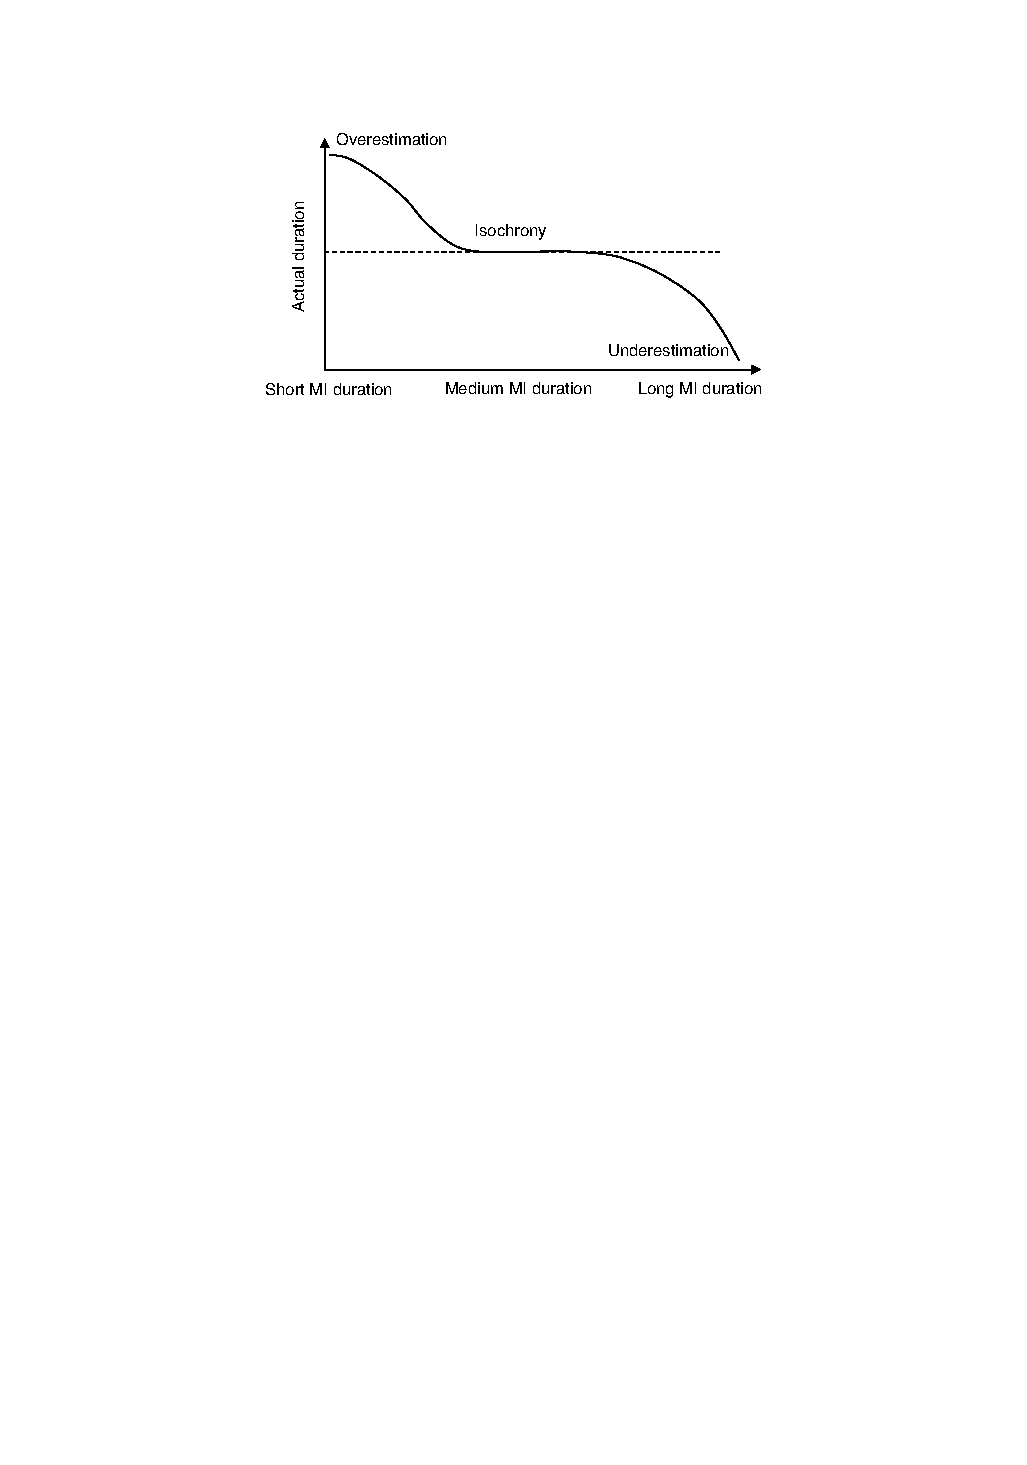
\includegraphics[width=0.75\linewidth]{assets/guillot_2012} 

}

\caption{Relationship between the actual duration of a movement and its mental representation. Figure from Guillot et al. (2012).}\label{fig:chronometry}
\end{figure}

In addition to mental chronometry, many authors in the second part of the XXth century turned to psychophysiological methods to investigate inner speech. The idea that the production of inner speech may involve the speech motor system is supported by many studies showing peripheral muscular activation during inner speech production (as reviewed for instance in Garrity, \protect\hyperlink{ref-garrity_electromyography_1977}{1977}; Locke, \protect\hyperlink{ref-locke_subvocal_1970-1}{1970}; Sokolov, \protect\hyperlink{ref-sokolov_inner_1972}{1972}). Among these, Faaborg-Andersen, Edfeldt, \& Nykøbing (\protect\hyperlink{ref-faaborg-andersen_electromyography_1958}{1958}) and McGuigan \& Rodier (\protect\hyperlink{ref-mcguigan_effects_1968}{1968}) found an increase in peripheral muscular activity in the speech muscles during silent reading. Interestingly, this activity was more strongly marked for novice readers or for difficult material. Locke \& Fehr (\protect\hyperlink{ref-locke_subvocal_1970}{1970}) compared the electromyographic correlates of subvocal speech (inner speech) during the (visual) presentation and rehearsal of disyllabic words that either contain or do not contain labial phonemes. They observed a greater EMG amplitude recorded over a \enquote{chin-lip} site during the presentation and rehearsal of labial words than for non-labial words.

In his seminal book, Sokolov (\protect\hyperlink{ref-sokolov_inner_1972}{1972}) meticulously describes a series of experiments conducted in order to examine the relation between inner speech and thought. Sokolov (\protect\hyperlink{ref-sokolov_inner_1972}{1972}) starts with a review of previous theories about the relation between speech and thought, before turning to the specific question of inner speech. He then presents his experimental work under two main parts. First, Sokolov (\protect\hyperlink{ref-sokolov_inner_1972}{1972}) used articulatory suppression\footnote{The expression \emph{articulatory suppression} usually refers to a task which requires participants to utter speech sounds (or to produce speech gestures without sound), so that this activity disrupts ongoing speech production processes.} to interfere with mental activity (e.g., perception, memorisation, thinking). Second, he used electromyography to investigate the involvement of the speech motor system during inner speech as well as in verbal and concrete thinking.

Summarising the studies using articulatory suppression, Sokolov (\protect\hyperlink{ref-sokolov_inner_1972}{1972}) notes that \enquote{mechanical retardation of external articulation (speech movements of lips and tongue) has an insignificant effect on the performance of mental tasks by adults; in many cases it has no effect at all. In children, the mechanical retardation of articulation has a noticeable negative effect} (p.152). This result is coherent with the idea of a progressive internalisation of inner speech, that would become more and more independent from the speech motor system throughout development (and thus less affected by motor constraints). However, Sokolov notes that articulated speech and verbal-auditory stimuli have a strong effect on memory (p.152). Moreover, Sokolov discusses some of his previous experimental work showing that motor interference (e.g., articulatory suppression) ceases to be efficient when the mental activity (inner speech) is automatised (e.g., rehearsing a poem learned by heart). In addition to age and expertise, Sokolov discusses findings from Teplov, who observed that the involvement of the speech motor system during inner speech might vary according to the \enquote{voluntariness} (deliberateness) of the speech to be produced. According to Teplov, the speech motor system would be necessarily involved during voluntary inner singing (a musical form of inner speech) whereas it may or may not be involved during involuntary inner singing (Sokolov, \protect\hyperlink{ref-sokolov_inner_1972}{1972}, p. 51).

Using electromyography, Sokolov (\protect\hyperlink{ref-sokolov_inner_1972}{1972}) also provided seminal observations that inner speech is involved during reading, to an extent that is directly related to the difficulty of the ongoing reading task (as observed previously by Faaborg-Andersen et al., \protect\hyperlink{ref-faaborg-andersen_electromyography_1958}{1958}). More precisely, he observed that the more difficult the task was, the stronger the \enquote{speech motor impulses} (i.e., the EMG amplitude) in the speech muscles. Moreover, the difficulty of the task was also related to the abbreviatedness of inner speech. Simpler reading tasks were associated with abbreviated (condensed)\footnote{Sokolov (\protect\hyperlink{ref-sokolov_inner_1972}{1972}) uses the term of \enquote{curtailment} for abbreviation (p.203).} inner speech whereas difficult tasks were associates with \enquote{unfolded} (expanded) inner speech, and sometimes externalised (overt) speech. Sokolov later says (on p.202):

\begin{quote}
\enquote{{[}\ldots{]} thus, it is evident that both the degree to which mental operations are automatized and the degree of complexity of the operations being performed can be assessed with a high degree of probability {[}confidence{]} on the basis of the intensity of hidden motor speech reactions.}
\end{quote}

Moreover, Sokolov observes that the muscular activity associated with inner speech production decreases when the verbal material is repeated many times (p.200-201). It increases again when new content is to be produced. For instance, he observes an important muscular activity during the reading of a new text, whereas this activity decreases when reading the text again. Interestingly, this reduction of peripheral muscular activity as a function of repetition may be countered by the instruction given to the participant. For instance, when the participant is given the instruction to \enquote{read it more attentively} or to \enquote{memorize it more accurately}, the reading of a known text results in similar peripheral muscular activity (in the speech muscles) as for the reading of a novel text (read without such instructions).

To summarise previous (i.e., anterior to Sokolov) research, articulatory suppression and electromyographic investigations conducted by Sokolov (\protect\hyperlink{ref-sokolov_inner_1972}{1972}), the involvement of the speech motor system during inner speech may vary according to the content of the verbal material, to characteristics of the task as well as to individual characteristics. More precisely, the intensity of \enquote{motor speech impulses} (in Sokolov's terms) may be intensified or reduced depending on i) the difficulty and novelty of the mental tasks being performed, ii) the degree of automatisation, iii) the inclusion of visual elements (whether the task is purely verbal or not), iv) individual disposition toward specific types of imagery. We can also add to these factors the age of the participant, with an involvement of the speech motor system being a decreasing function of age. Overall, these findings are coherent with the idea of a progressive internalisation of speech into inner speech, which lead Sokolov to state that \enquote{inner speech is nothing but speech to oneself} and that it can be considered as an internalisation, a psychological transformation or an \enquote{internal projection} of overt speech (Sokolov, \protect\hyperlink{ref-sokolov_inner_1972}{1972}). Sokolov concludes his work by stating that inner speech is \enquote{the principal mechanism of thought} and \enquote{an essential factor to human consciousness} (Sokolov, \protect\hyperlink{ref-sokolov_inner_1972}{1972}, p. 262).

Following seminal work by Jacobson (\protect\hyperlink{ref-jacobson_electrical_1931}{1931}) and Sokolov (\protect\hyperlink{ref-sokolov_inner_1972}{1972}), the 70s and 80s witnessed an upsurge of electromyographic studies of inner speech production. For instance, McGuigan \& Winstead (\protect\hyperlink{ref-mcguigan_discriminative_1974}{1974}) recorded both lip and tongue EMG activity during the reading, viewing, memorising or recalling of either bilabial or lingual-alveaolar verbal material. They observed a double dissociation with the bilabial material being associated with a greater EMG amplitude recorded over the lip and the lingual-alveolar being associated being associated with a greater EMG amplitude recorded over the tongue (whereas EMG amplitude recorded over the arm or the leg did not show these condition-specific changes). Similarly, Garrity (\protect\hyperlink{ref-garrity_measurement_1975}{1975}) observed a greater lip activity during the covert production of labial items than during the covert production of nonlabial items. Importantly, in her review, Garrity (\protect\hyperlink{ref-garrity_electromyography_1977}{1977}) highlights some methodological limitations to EMG studies of inner speech and makes practical recommendations to avoid these pitfalls (see Box \ref{garrity}). McGuigan \& Dollins (\protect\hyperlink{ref-mcguigan_patterns_1989}{1989}) recorded EMG activity over the lip and the tongue during the processing of single phonemes (\enquote{P} vs.~\enquote{T}) and observed a greater activity of the lip during the processing of \enquote{P} and a greater amplitude of the tongue during the processing of \enquote{T}, confirming previous results suggesting a discriminative relationship between the content of inner speech and its peripheral muscular correlates. In the same vein, Livesay, Liebke, Samaras, \& Stanley (\protect\hyperlink{ref-livesay_covert_1996}{1996}) recorded EMG over the lip during the production of inner speech and during the visualisation of non-linguistic material and observed a greater EMG amplitude recorded over the lip during the production of inner speech. Interestingly, discussing the EMG correlates of inner speech (and motor imagery), MacKay (\protect\hyperlink{ref-mackay_constraints_1992}{1992}) remarks that this \enquote{EMG activity invariably precedes by a few milliseconds the full blown muscle activity that occurs during normal movements} (p.133). Taken together, these results suggest that the peripheral muscular correlates of inner speech are content-specific and that it should be possible to use electromyographic measurements to identify or \enquote{decode} the content of inner speech. This idea has been corroborated by recent work showing that surface EMG can be used to discriminate between different digits produced innerly, and that it could be used as a silent communication device (e.g., Kapur, Kapur, \& Maes, \protect\hyperlink{ref-kapur_alterego_2018}{2018}). However, other teams find contrasting results (e.g., our results in Chapter \ref{chap5} or Meltzner et al., \protect\hyperlink{ref-meltzner_speech_2008}{2008}) and we discuss this issue further in Chapter \ref{chap5}.

\vspace{2mm}

\begin{mybox}[label = garrity]{Proper control conditions in EMG studies of inner speech production}

Many of the studies that used EMG to investigate the motor correlates of inner speech production concluded on the involvement of the speech motor system based on a difference in EMG amplitude when contrasting a period of inner speech production with a resting period. However, as highlighted by Garrity (1977), it is usually not enough to show an increase of speech muscle activity during inner speech to conclude that this activation is related to inner speech production.\\

Three sorts of inference can be made through electromyographic studies of inner speech production, depending on the stringency of the control procedure. The stronger sort of inference is permitted by highlighting a discriminative pattern during covert speech production, as for instance when demonstrating a dissociation between different speech muscles during the production of speech sounds of different phonemic class (e.g, contrasting labial versus non-labial words). Other (weaker) types of control procedures include i) comparing the EMG activity during covert speech production to a baseline period (without contrasting phonemic classes in covert speech utterances), or ii) comparing the activity of speech-related and non-speech related (e.g., forearm) muscle activity. Ideally, these controls should be combined by recording and contrasting speech and non-speech related muscles in different conditions (e.g., rest, covert speech, overt speech) of pronunciation of different speech sounds classes (e.g., labial versus non-labial).

\end{mybox}

Besides mental chronometry and electromyography, the second part of the last century also witnessed a revival of introspective methods, with the aim of refining the description of the phenomenological properties of inner speech. For instance, the use of the experience sampling methodology (ESM, Csikszentmihalyi \& Larson, \protect\hyperlink{ref-csikszentmihalyi_validity_1987}{1987}) permitted to examine inner speech in a naturalistic environment and to assess its frequency, forms and usages. For instance, Klinger \& Cox (\protect\hyperlink{ref-klinger_dimensions_1987}{1987}) asked 29 students to carry a beeper that probed them randomly to described the properties of their mental activity. They observed that around 51\% of the samples contained some form of internal monologue. Using a modified version of the ESM known as the \emph{descriptive experience sampling} methodology (DES, Hurlburt, \protect\hyperlink{ref-Hurlburt2011}{2011}; Hurlburt \& Akhter, \protect\hyperlink{ref-hurlburt_descriptive_2006}{2006}; Hurlburt \& Heavey, \protect\hyperlink{ref-Hurlburt2001}{2001}; Hurlburt, Heavey, \& Kelsey, \protect\hyperlink{ref-Hurlburt2013}{2013})\footnote{The DES differs from the classical random-beeping strategy in that the participant, in addition to being probed several times a day (e.g., until 8-10 times a day), also has to meet with the experimenter at the end of the study. During this \enquote{expositional interview}, the experimenter and the participant work together to clarify the meaning of these reported inner experiences as well as to contextualise them.}, Heavey \& Hurlburt (\protect\hyperlink{ref-heavey_phenomena_2008}{2008}) assessed the frequency of common inner experiences and found that inner speech fills around 25\% of our conscious inner life. Their results suggest that the rest of our inner experience is filled with four other main components: inner seeing, feeling (i.e., affective experiences such as happiness or sadness), sensory awareness (i.e., paying attention to immediate sensations such as hunger), and unsymbolised thinking (i.e., thinking without words, images, or any other symbol). Thus, our inner life is not only filled with language but other forms of thinking (defined broadly, as before, as any sort of mental activity) may coexist (for a review and synthesis of DES findings, see Hurlburt, \protect\hyperlink{ref-Hurlburt2011}{2011}; Hurlburt et al., \protect\hyperlink{ref-Hurlburt2013}{2013}).

Moreover, based on historical and DES data, Hurlburt (\protect\hyperlink{ref-Hurlburt2011}{2011}) argues for a distinction between two forms of inner speech (or two phenomenological aspects of inner speech). According to Hurlburt, it is possible to make a distinction between the phenomenon of \emph{inner speaking} and the phenomenon \emph{inner hearing}, whose feelings would be similar to talking in a tape recorder and to hear your voice played back, respectively (Hurlburt et al., \protect\hyperlink{ref-Hurlburt2013}{2013}). Hurlburt, Alderson-Day, Kühn, \& Fernyhough (\protect\hyperlink{ref-hurlburt_exploring_2016}{2016}) provide data suggesting that these two phenomena may have distinct neural correlates (but see Lœvenbruck et al., \protect\hyperlink{ref-loevenbruck_cognitive_2018}{2018}, for another stance on these data). The distinction between inner speaking and inner hearing echoes previous distinctions (e.g., MacKay, \protect\hyperlink{ref-mackay_constraints_1992}{1992}) such as the one between the \enquote{generative component} (i.e., the feeling of producing speech) and the \enquote{auditory component} (i.e., the feeling of hearing speech) and the distinction between the \emph{inner ear} and the \emph{inner voice} in studies of working memory (e.g., Baddeley, Lewis, \& Vallar, \protect\hyperlink{ref-baddeley_exploring_1984}{1984}; Buchsbaum, \protect\hyperlink{ref-buchsbaum_role_2013}{2013}).

Another source of information concerning the nature of inner speech comes from the study of errors produced during inner speech. For instance, Dell \& Repka (\protect\hyperlink{ref-dell_errors_1992}{1992}) asked participants to produce tongue twisters (such as \enquote{Unique New York}) either aloud or mentally and to report the type of error they made (if any). They observed that the participants made the same kind of errors in overt and inner speech, indicating that inner speech, like overt speech, may involve the same kind of units (e.g., phonological, morphological or lexical units). As suggested by Oppenheim \& Dell (\protect\hyperlink{ref-oppenheim_inner_2008}{2008}), the similarity of errors found in inner speech and overt speech indicates that slips of the tongues are not really slip of the tongue, but rather slips of speech planning. More recently, Oppenheim \& Dell (\protect\hyperlink{ref-oppenheim_inner_2008}{2008}) shown that the covert recitation of tongue twisters is accompanied by the lexical bias also observed in overt production but do not show the phonemic similarity bias (i.e., the tendency to exchange phonemes with common articulatory features) observed in overt speech. This observation lead Oppenheim \& Dell (\protect\hyperlink{ref-oppenheim_inner_2008}{2008}) and Oppenheim \& Dell (\protect\hyperlink{ref-oppenheim_motor_2010}{2010}) to claim that although inner speech is specified at a lexical level, it is impoverished at the featural (articulatory) level. In contrast to these results, however, Corley, Brocklehurst, \& Moat (\protect\hyperlink{ref-corley_error_2011}{2011}) found the phonemic similarity effect to be present in inner speech, suggesting that inner speech is not necessarily impoverished at the articulatory level.

Besides, some studies tried to directly interfere with the motor system in order to make causal claims about inner speech and the role of the motor system during inner speech production. These studies include for instance articulatory suppression studies (see our more detailed discussion of articulatory suppression findings in Chapter \ref{chap6}) at the behavioural level and transcranial magnetic stimulation studies at the neural level. Using repetitive transcranial magnetic stimulation, Aziz-Zadeh, Cattaneo, Rochat, \& Rizzolatti (\protect\hyperlink{ref-Aziz-Zadeh2005}{2005}) induced both overt and covert speech arrests (i.e., a transient inability to produce speech) by targeting both a motor (posterior) and a \enquote{non-motor} (anterior, corresponding to the inferior frontal gyrus) area of the left hemisphere. Many studies investigated the cerebral correlates of both overt speech and inner speech and showed that both modes involve language areas in the left hemisphere, such as motor and premotor cortices in the frontal lobe, including Broca's areas or the left inferior frontal gyrus (IFG). These studies also highlight the involvement of regions involved in speech perception such as auditory areas, Wernicke's areas and the left parietal lobule, an associative region (for review, see Geva, \protect\hyperlink{ref-geva_inner_2018}{2018}; Lœvenbruck et al., \protect\hyperlink{ref-loevenbruck_cognitive_2018}{2018}; Perrone-Bertolotti, Rapin, Lachaux, Baciu, \& Lœvenbruck, \protect\hyperlink{ref-Perrone-Bertolotti2014}{2014}). Ackermann \& Riecker (\protect\hyperlink{ref-ackermann_contribution_2004}{2004}) also observed an activation of the left supplementary motor area (SMA), left primary motor cortex (M1), and right cerebellum during covert speech. Activation of the primary motor cortex during inner speech (and more broadly, during imagined action) is still controversial and may depend on characteristics of the task (e.g., instructions given to the participant, characteristics of the content/material to be produced) and the type of inner speech. Overall, activation in the motor, premotor and sensory cortices is known to be stronger during overt speech than inner speech, supporting the idea that inner speech may be considered on a continuum from inner speech to overt speech. However, inner speech also involves additional regions in comparison to overt speech (e.g., Basho, Palmer, Rubio, Wulfeck, \& Müller, \protect\hyperlink{ref-basho_effects_2007}{2007}). Importantly, inner speech recruits regions involved in the inhibition of overt responses (e.g., cingulate gyrus, left middle frontal gyrus, pre-SMA). To sum up, neuroimaging studies support the idea that inner speech may be conceived as simulated speech, involving similar motor and sensory areas, but to a lesser extent than overt speech. In addition to common areas, inner speech also involve supplementary areas related to the inhibition of overt responses, supporting the idea that inner speech is simulated overt speech resulting from inhibited speech acts (for more details, see the cerebral landscape of (wilful) inner speech production proposed in the next section, as well as recent reviews, Alderson-Day \& Fernyhough, \protect\hyperlink{ref-alderson-day_inner_2015}{2015}; Lœvenbruck et al., \protect\hyperlink{ref-loevenbruck_cognitive_2018}{2018}; Perrone-Bertolotti et al., \protect\hyperlink{ref-Perrone-Bertolotti2014}{2014}).

More recently, technical and methodological developments from the field of neural engineering offered new ways of investigating inner speech. Several teams are conducting research with the aim of \enquote{decoding inner speech}, that is, of deciphering the content of inner speech based on neurophysiological signals. For instance, Martin et al. (\protect\hyperlink{ref-martin_decoding_2014}{2014}) recorded electrocorticographic (ECoG) signals from epileptic patients performing either overt or covert reading tasks. Then, they built a neural decoding model capable of reconstructing the spectrotemporal auditory features of the overt reading task and evaluated whether this model could reconstruct auditory speech features in the covert reading condition. They demonstrated that it is possible to decode (or to infer) inner speech content by using a model learned on corresponding overt speech data, with the superior temporal gyrus as well as the pre- and post-central gyrus providing the most diagnostic information. Martin et al. (\protect\hyperlink{ref-martin_word_2016}{2016}) also used ECoG recording from the temporal lobe and sensorimotor cortex and showed that it is possible to reach a relatively high accuracy level in a two-class classification framework and above-chance accuracy levels in classifying fifteen word-pairs based on ECoG signals (for a recent review, see Martin, Iturrate, Millán, Knight, \& Pasley, \protect\hyperlink{ref-martin_decoding_2018}{2018}). Using a different technic, Kapur et al. (\protect\hyperlink{ref-kapur_alterego_2018}{2018}) developed a wearable device capable of discriminating inner speech content based on surface electromyographic signals. They showed that their method was able to discriminate with relatively high accuracy digits (between 0 and 9) that were produced covertly. However, as mentioned previously, other teams find contrasting results (e.g., our results in Chapter \ref{chap5} or Meltzner et al., \protect\hyperlink{ref-meltzner_speech_2008}{2008}) and we discuss this issue further in the discussion of Chapter \ref{chap5}. Overall, these results show that it is presently possible to decode inner speech based on neurophysiological signals above chance levels. Although these results currently stand for limited vocabulary sets, it might soon be possible to have fully operational online inner speech decoding systems. However, the issue of prediction and the issue of explanation are not reducible one to the other and although we might be in situation of correctly inferring (predicting) the content of inner speech based on neurophysiologial signals, some theoretical issues still need to be resolved (we turn to theoretical propositions in the next section).

\begin{landscape}

\begin{figure}

{\centering 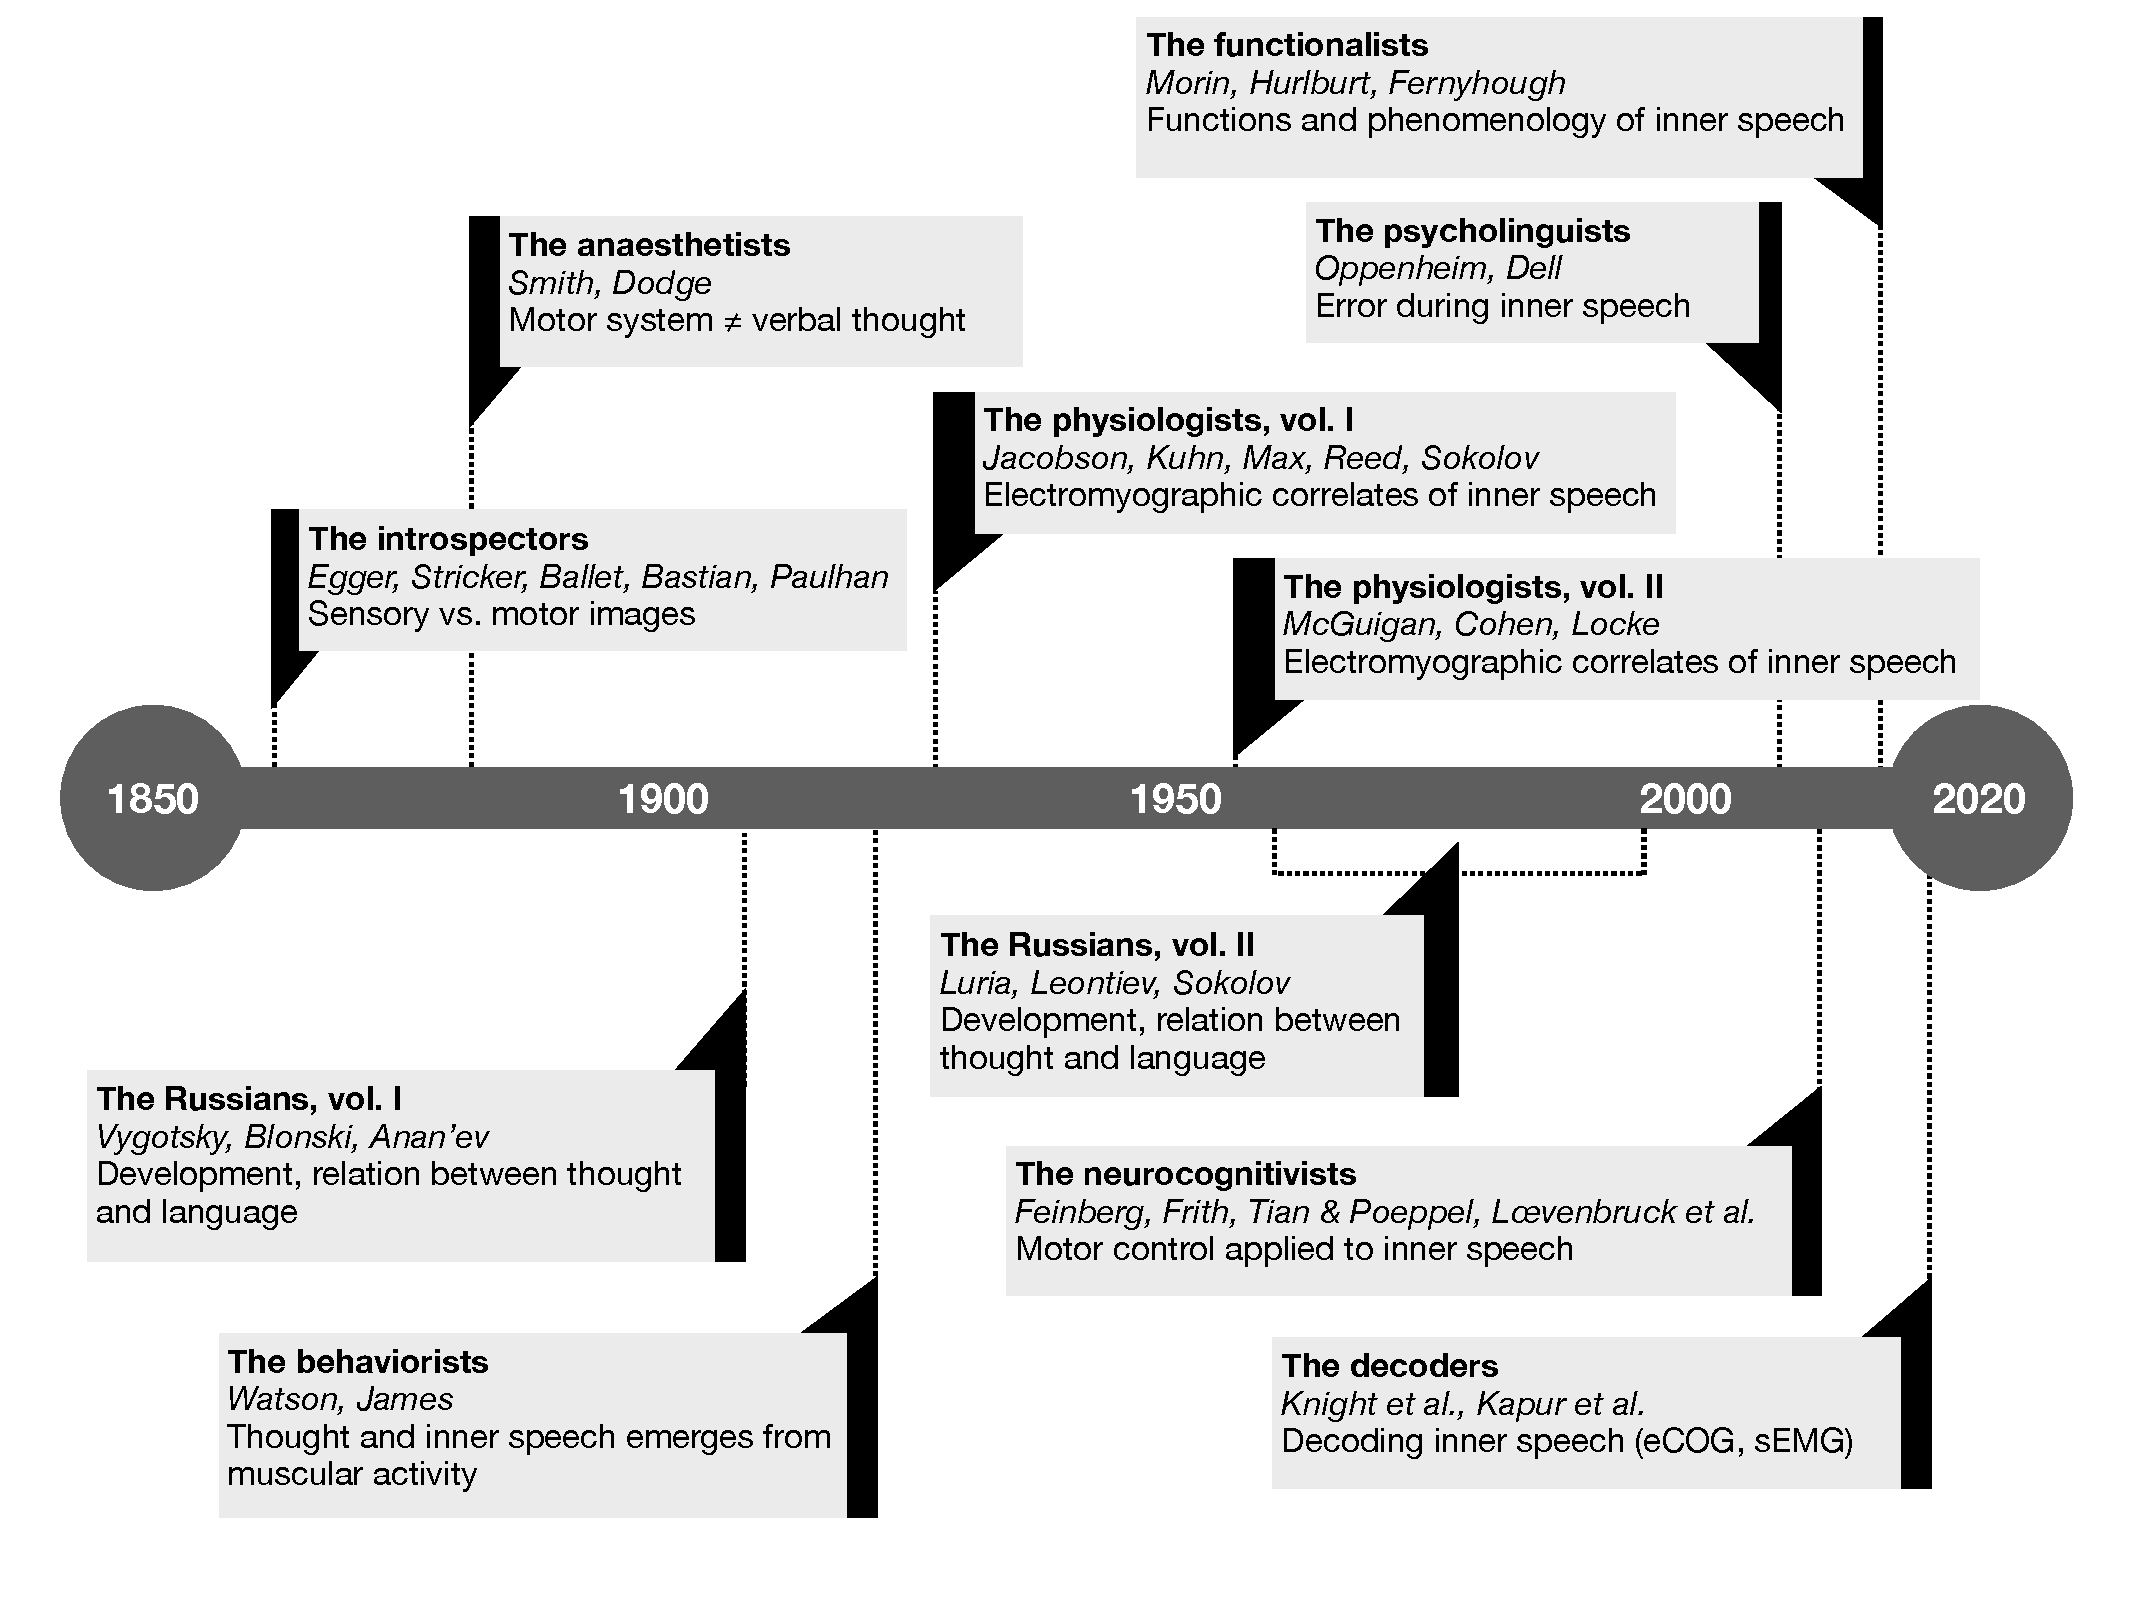
\includegraphics[width=1\linewidth]{assets/timeline} 

}

\caption{Non-exhaustive overview of inner speech research from 1850 to present days, depicting some representative names and their main contribution. NB: dates represent the starting point of some contribution rather than the precise temporal location of the contribution (as most contributions extend on a period of several years or decades).}\label{fig:timeline}
\end{figure}

\end{landscape}

In this section, we briefly reviewed the history of inner speech research carried out over the last 170 years (from 1850 to present days) to give an overview of the evolution of ideas and methods related to inner speech research (these investigations are summarised in a non-exhaustive timeline presented in Figure \ref{fig:timeline}). The interested reader will find supplementary information in more comprehensive reviews, theses, and books (e.g., Alderson-Day \& Fernyhough, \protect\hyperlink{ref-alderson-day_inner_2015}{2015}; Fernyhough, \protect\hyperlink{ref-fernyhough_voices_2016}{2016}; Gregory, \protect\hyperlink{ref-gregory_inner_2017}{2017}; Langland-Hassan \& Vicente, \protect\hyperlink{ref-langland-hassan_inner_2018}{2018}; Lœvenbruck, \protect\hyperlink{ref-loevenbruck_loquor_2019}{2019}; Lœvenbruck et al., \protect\hyperlink{ref-loevenbruck_cognitive_2018}{2018}; Perrone-Bertolotti et al., \protect\hyperlink{ref-Perrone-Bertolotti2014}{2014}; Rapin, \protect\hyperlink{ref-Rapin2011}{2011}; Smadja, \protect\hyperlink{ref-smadja_parole_2019}{2019}). In the next section, we discuss the most recent and important theoretical positions about the nature and production of inner speech.

\hypertarget{inner-speech-theories}{%
\subsection{Theoretical perspectives on inner speech}\label{inner-speech-theories}}

\hypertarget{the-psycholinguistics-perspective}{%
\subsubsection{The psycholinguistics perspective}\label{the-psycholinguistics-perspective}}

How do we (humans) produce speech? At a biomechanical level, producing speech means coordinating a complex dynamic system (i.e., the ensemble of speech muscles and organs) to produce slight perturbations of the air flow (sound waves). At a psychological level, speech production can be said to consist in the translation of thoughts into speech, with the goal of communicating information. Before being communicated however, the information of interest is submitted to several important transformations.

Although speech production is an everyday phenomenon, the way this process is exactly performed is still the subject of lively debates. However, current models generally agree with the core steps occurring during speech production. Willem Levelt (Levelt, \protect\hyperlink{ref-levelt_speaking_1989}{1989}, \protect\hyperlink{ref-brown_producing_2000}{2000}) proposed an influential psycholinguistic model of speech production (see Figure \ref{fig:levelt}). According to this model, speech production can be described at three levels: \emph{conceptualisation}, \emph{formulation} and \emph{articulation}. The first step is managed by a component called the \emph{conceptualizer}, and consists in selecting a conceptual message to be produced (\emph{message generation}). In other words, the speaker conceives a comunicative intention that she wishes to reveal to an interlocutor. This \emph{preverbal message} is then forwarded to another component, the \emph{formulator}, that handles both \emph{grammatical encoding} (i.e., selecting the appropriate word or \emph{lemma}) and \emph{phonological encoding} (i.e., selecting the appropriate speech sounds). During \emph{grammatical encoding}, \emph{lemmas} are retrieved from the \emph{lexicon} and are ordered in a syntactical appropriate way, giving the message its \emph{surface structure}. During \emph{phonological encoding}, the message is given its phonetic or articulatory characteristics. At this stage, phonemes are grouped into pronounceable syllables. Then, each syllable is associated with an \emph{articulatory program}, composed of an ensemble of \emph{articulatory gestures} (i.e., coordinative structures of movements). These articulatory programs are stored in the \emph{syllabary}. In brief, the \emph{formulator} component transforms a \emph{preverbal message} into a linguistic object. Finally, the phonetic plan is forwarded to the \emph{articulator}, responsible for the activation of \emph{articulatory gestures}, to be executed by the speech \emph{articulators} (e.g., tongue, lips, jaw).\footnote{This model permits to explain how a communicative intention is transformed into speech acts. However, it does not explicitly account for how speech acts are executed by the articulators. In Chapter \ref{chap2}, we briefly introduce some of the cores principles related to the biomechanics of speech production.}

\begin{figure}

{\centering 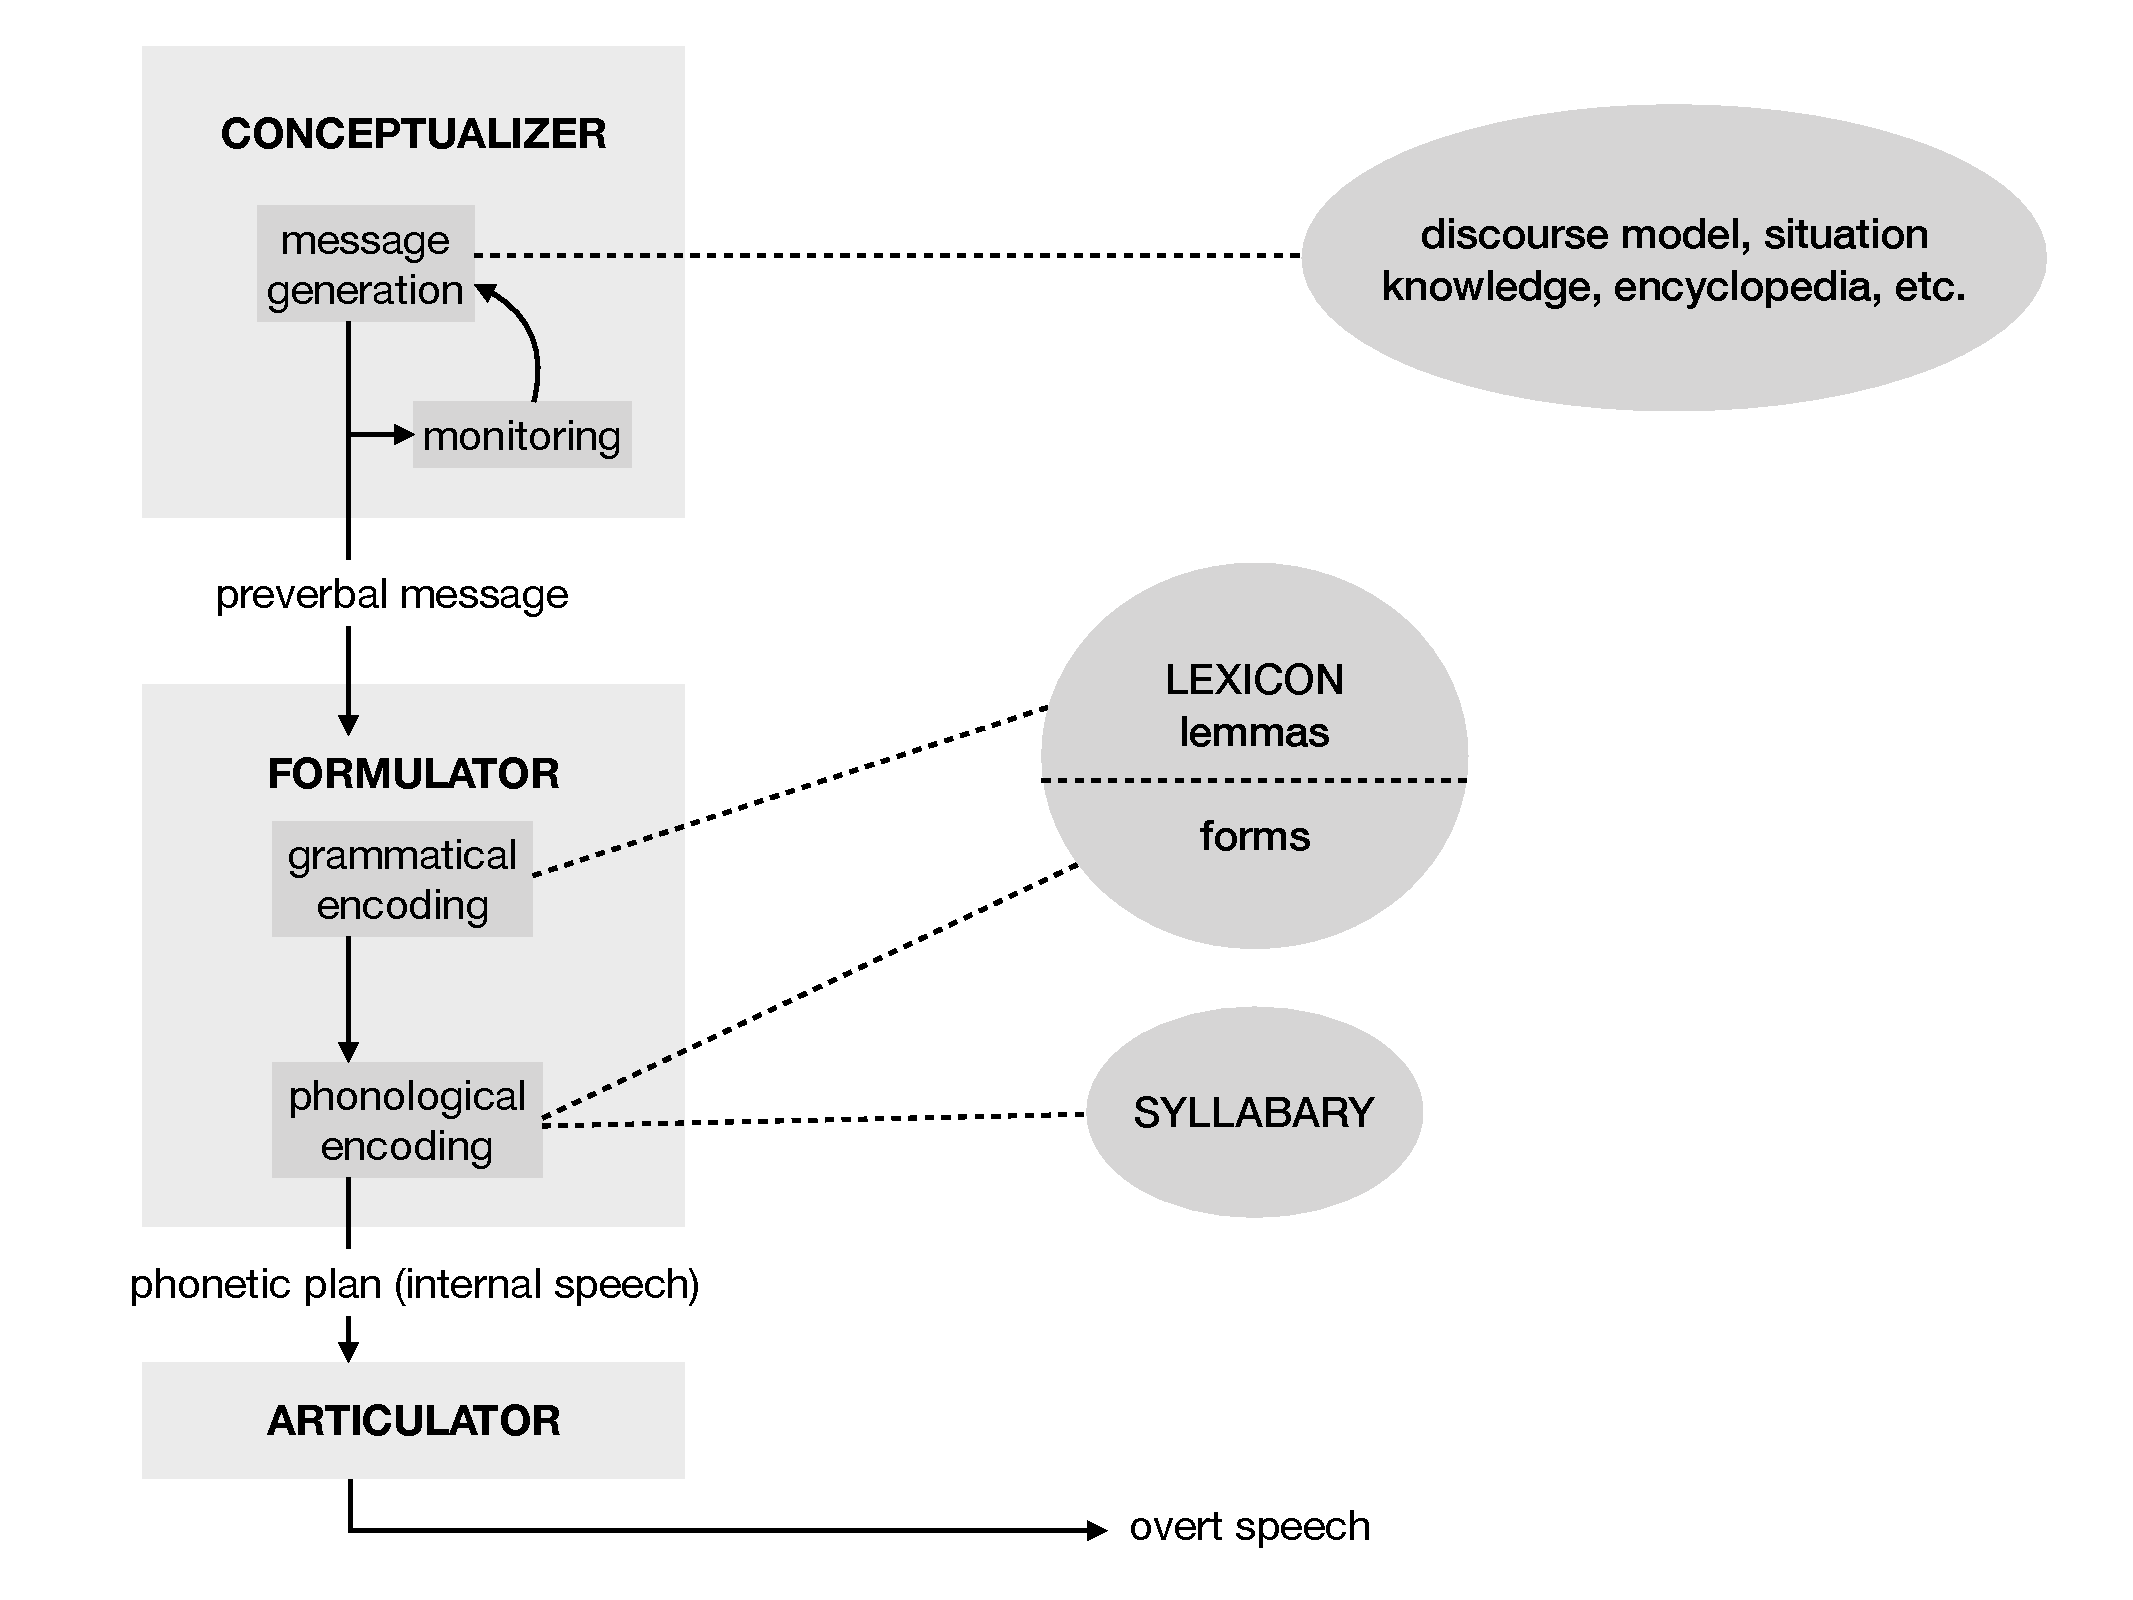
\includegraphics[width=0.75\linewidth]{assets/levelt} 

}

\caption{Illustration of Levelt's (1989, 2000) model of speech production.}\label{fig:levelt}
\end{figure}

Interestingly, in this model, inner speech is thought to correspond to the phonetic plan. In other words, inner speech is considered as a plan for overt speech, something that precedes overt speech. The idea that inner speech is some sort of a plan for overt speech is widespread in psycholinguistics. According to Levelt, Roelofs, \& Meyer (\protect\hyperlink{ref-levelt_theory_1999}{1999}), we produce inner speech in the same way we produce overt speech, except that articulation is absent (we already encountered the \emph{continuum hypothesis} previously). One of the role of this covert mode in speak production would be to allow for monitoring planned speech for errors (e.g., Hartsuiker \& Kolk, \protect\hyperlink{ref-hartsuiker_error_2001}{2001}; Levelt, \protect\hyperlink{ref-levelt_monitoring_1983}{1983}). For some authors, inner speech would only be a by-product of the need of the speaker to control overt speech (e.g., Oppenheim, \protect\hyperlink{ref-oppenheim_inner_2013}{2013}). If we are to accept the \emph{continuum hypothesis}, according to which there is a continuum between inner speech and overt speech, we are faced with the question of the locus of truncation. If both inner and overt speech lie on the same continuum, where inner speech ceases to be inner speech?

\begin{figure}

{\centering 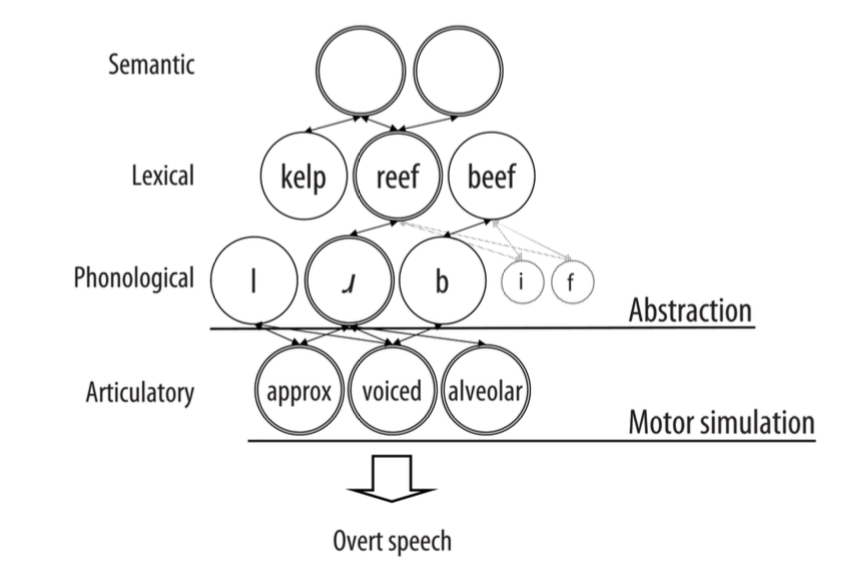
\includegraphics[width=0.66\linewidth]{assets/oppenheim} 

}

\caption{Hypotheses regarding inner speech's locus of generation. Depending on the framework, inner speech is thought to be specified at an articulatory level (motor simulation view) or not to be (abstraction view). Figure from Oppenheim \& Dell (2010).}\label{fig:oppenheim}
\end{figure}

Oppenheim \& Dell (\protect\hyperlink{ref-oppenheim_inner_2008}{2008}) listed and examined three hypotheses regarding this issue. First, inner speech may be exactly like overt speech, except that articulators are not moved. Second inner speech may be impoverished at a surface level (featural representations). Third, inner speech may be impoverished at a deeper (e.g., lexical level) with relatively intact phonological or articulatory features. As discussed in the previous section, the observation that only the lexical bias (but not the phonemic similarity effect) was found in inner speech lead Oppenheim \& Dell (\protect\hyperlink{ref-oppenheim_inner_2008}{2008}) to claim that inner speech was impoverished at a featural (articulatory) level. Oppenheim \& Dell (\protect\hyperlink{ref-oppenheim_motor_2010}{2010}) further added that theories about inner speech may be classified into two main classes (cf.~Figure \ref{fig:oppenheim}). According to the first class of theories, referred to as the \emph{motor simulation view}, inner speech would be like overt speech, except that articulators are not moved (this represents the first hypothesis listed in Oppenheim \& Dell, \protect\hyperlink{ref-oppenheim_inner_2008}{2008}). The second class of theories is known as the \emph{abstraction view} and considers inner speech to be the consequence \enquote{of the activation of abstract linguistic representations} (Oppenheim \& Dell, \protect\hyperlink{ref-oppenheim_motor_2010}{2010}). After reviewing supporting and contradictory evidence for each view, Oppenheim \& Dell (\protect\hyperlink{ref-oppenheim_motor_2010}{2010}) suggest a reconciliatory hypothesis, according to which the abstractiveness of inner speech would be \emph{flexible.} More precisely, the flexible abstraction account postulates inner speech would only be specified at a phonological level but that this phonological level would be affected by articulation. In support of this idea, Oppenheim \& Dell (\protect\hyperlink{ref-oppenheim_motor_2010}{2010}) observed that mouthed inner speech showed both a lexical bias and a phonemic similarity effect, which was not the case for unmouthed inner speech.

\hypertarget{the-motor-theory-of-voluntary-thinking}{%
\subsubsection{The motor theory of voluntary thinking}\label{the-motor-theory-of-voluntary-thinking}}

The \emph{motor theory of voluntary thinking} (MTVT, Cohen, \protect\hyperlink{ref-cohen_motor_1986}{1986}) aims to explain how thinking and the experience of volition can emerge from motor activity. Cohen first notes that a critical aspect of motor theories is that they rely on peripheral motor feedback (i.e., afferent feedback from the contraction of the muscles). However, he then suggests that although motor feedback might be necessary at the initial stages of an internalised action (e.g., inner speech), this feedback might become unnecessary through repeated associations that would \enquote{short-circuit connections within the central nervous system} (Cohen, \protect\hyperlink{ref-cohen_motor_1986}{1986}, p. 21). According to the MTVT, motor activity would be necessary for mental experiences without external sensation (i.e., for imagery or thoughts). More precisely, Cohen (\protect\hyperlink{ref-cohen_motor_1986}{1986}) suggests that inner speech (or rather, the sensory percepts associated with inner speech) might be explained by its associations with motor activity. Indeed, according to Cohen (\protect\hyperlink{ref-cohen_motor_1986}{1986}), \enquote{associations between one's voice and kinesthetic sensations from one's speech musculature are very specific, consistent, and frequently repeated} (p.22). Therefore, slight (unconscious) contractions of the speech musculature might evoke speech auditory images. In support of this idea, Cohen reports the results of an experiment lead by Hefferline \& Perera (\protect\hyperlink{ref-hefferline_proprioceptive_1963}{1963}):

\begin{quote}
\enquote{when the subject occasionnaly emitted an invisibly small thumb twitch (detected electromyographically), he received a tone as a signal to press a key. After several conditioning sessions, the tone was progressively diminished to zero. The subject nevertheless continued to press the key whenever he emitted a thumb twitch, and he reported that he still heard the tone.}
\end{quote}

These observations support the idea that motor activity (and kinaesthetic feedback) might, after frequent association, evoke auditory sensations. Cohen then moves to a presentation of the motor theory of attention, according to which motor activity allows oneself to emphasise (or weight) one aspect of perception over another. According to Cohen, the MTVT, albeit not suggesting that motor activity for any sort of mental image or thought, suggests that motor feedback \emph{can} evoke mental images and thoughts (e.g., via the principle of association discussed above) and that motor activity is responsible for the experience of volition in thinking. The MTVT suggests that thoughts that are experienced voluntary (e.g., rehearsing a novel phone number) are accompanid by motor activity whereas involuntary thoughts (e.g., intrusive thoughts or ruminative thoughts) are not. Interestingly, Cohen also suggests that \enquote{a thought may appear to be effortless because no motor activation is involved, or because the motor activity is of an automatic nature} (p.27). Cohen interprets the effect of distraction on the implication of the motor system during motor imagery (and inner speech) in terms of attentional sharing, building upon Norman \& Shallice (\protect\hyperlink{ref-norman_attention_1986}{1986})'s work:

\begin{quote}
\enquote{In order to rehearse a telephone number one would simply \enquote{speak} the numbers covertly -- that is, activate the appropriate speech motor patterns, but too slightly to produce audible speech. To take the case of rehearsing a telephone number a step further, consider that the person is being distracted by loud music. Because the music would be competing for his attention, he would have to increase the amplitude of his rehearsal by increasing the speech motor activity, perhaps ot the point of making actual lip and tongue movements. Were the music loud he might have to speak the numbers aloud so that the numbers would capture enough of his awareness to remain in his short-term memory.}
\end{quote}

This idea is consistent with some work showing a greater implication of the speech motor system during cognitively demanding tasks (e.g., Sokolov, \protect\hyperlink{ref-sokolov_inner_1972}{1972}; McGuigan \& Rodier, \protect\hyperlink{ref-mcguigan_effects_1968}{1968}) and provides a mechanism to explain these observations (but see our own theoretical interpretation in the next section). To sum up, the MTVT suggests that all voluntary images and thoughts are associated with motor activity and that \enquote{deliberate inner speech is based\footnote{NB: "based" is used here in a developmental sense (cf.~the beginning of this section).} on the appropriate covert activity in the speech musculature} (Cohen, \protect\hyperlink{ref-cohen_motor_1986}{1986}, pp. 45--46).

\hypertarget{predictive-and-motor-control-accounts-of-inner-speech}{%
\subsubsection{Predictive and motor control account(s) of inner speech}\label{predictive-and-motor-control-accounts-of-inner-speech}}

Speech production requires the fine-grained timing and coordination of complex sequences of movements (cf.~biomechanical aspects of speech production in Chapter \ref{chap2}) and can therefore be considered in a common conceptual framework as with other forms of motor actions. Complex motor actions have been successfully modelled in a motor control framework (e.g., Kawato, Furukawa, \& Suzuki, \protect\hyperlink{ref-kawato_hierarchical_1987}{1987}; Kawato, \protect\hyperlink{ref-kawato_internal_1999}{1999}; Wolpert, Ghahramani, \& Jordan, \protect\hyperlink{ref-wolpert_internal_1995}{1995}; Wolpert, \protect\hyperlink{ref-wolpert_computational_1997}{1997}). Motor control models describe how the central nervous system and the musculoskeletal system interact in order perform motor actions. Applied to speech production, these models describe how humans generate and regulate speech acts (for an introduction to motor control models and a review of speech motor control models, see Parrell, Lammert, Ciccarelli, \& Quatieri, \protect\hyperlink{ref-parrell_current_2019}{2019}).

\begin{figure}

{\centering 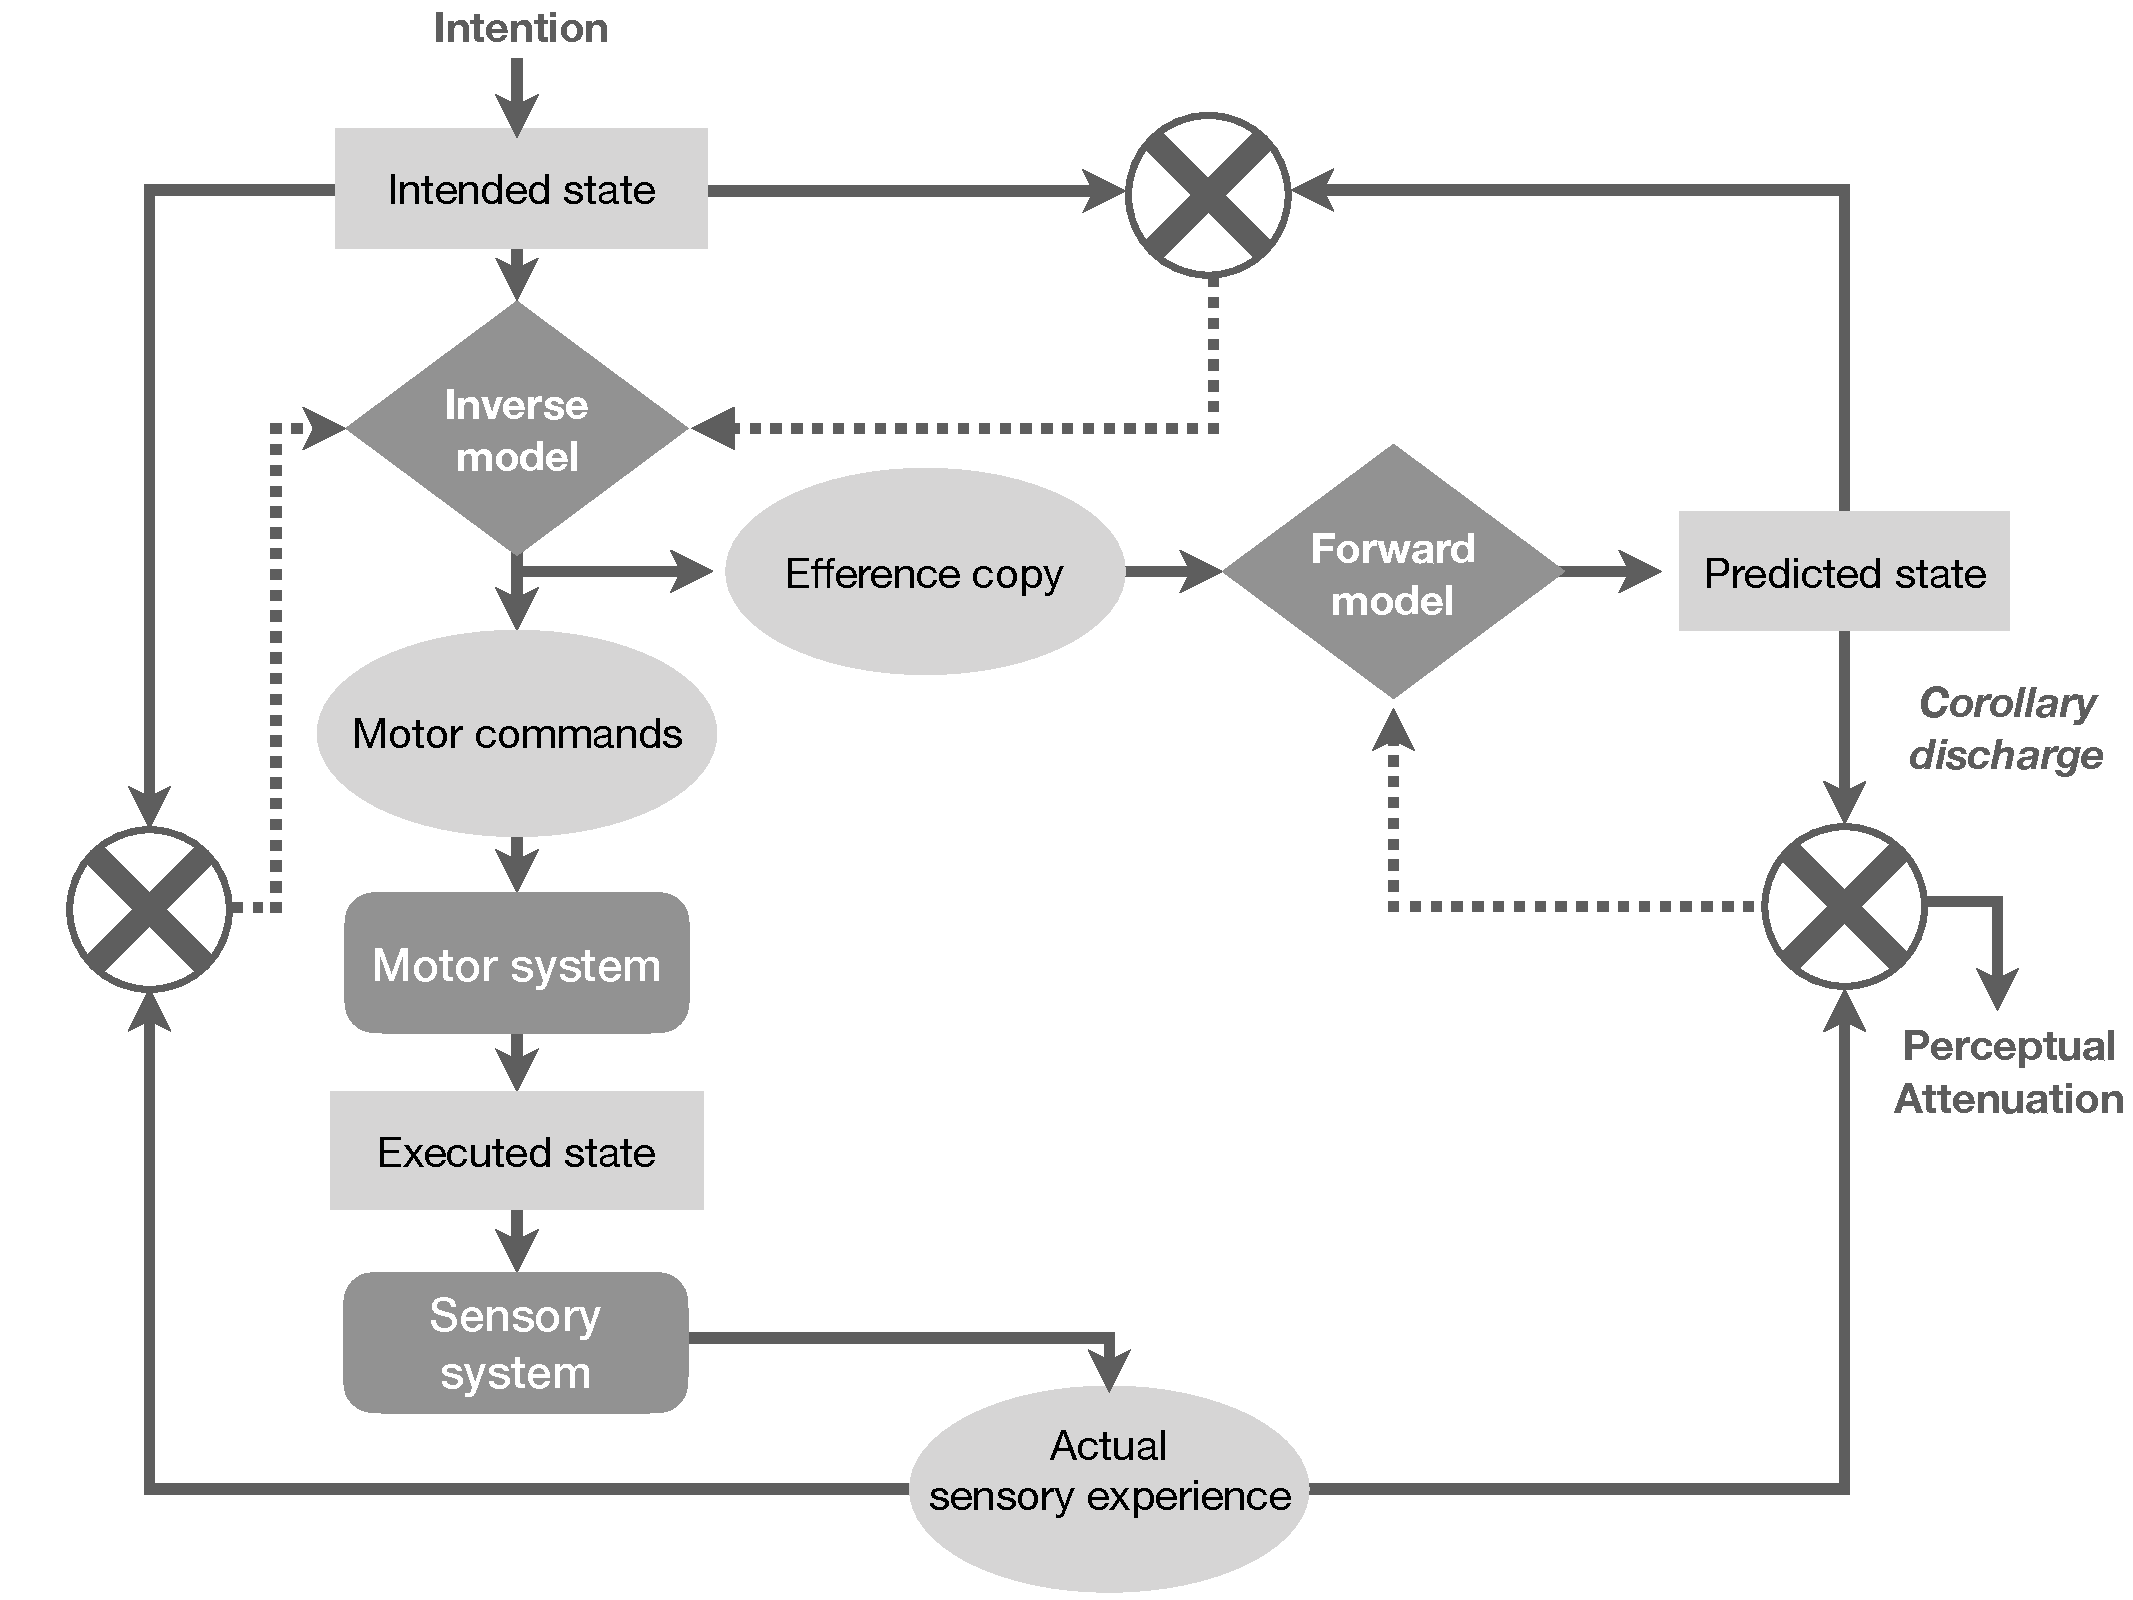
\includegraphics[width=0.75\linewidth]{assets/motor_control} 

}

\caption{A forward model of motor control. Crossed circles represent comparators (see text for explanation). Figure adapted from Rapin et al. (2013).}\label{fig:motorcontrol}
\end{figure}

Motor control models generally assume two types of interacting \emph{internal models}: a \emph{forward model} that is used to predict the consequences of some planned action and an \emph{inverse model} that is used to compute (to predict) the necessary movements to attain some goal (cf.~Box \ref{model}). As can be seen from Figure \ref{fig:motorcontrol}, the inverse model is first used to compute the necessary motor commands to attain some intended state (e.g., producing the /i/ vowel). When motor commands are sent to the motor system, a copy of these motor commands (known as the \emph{efference copy}) is sent to a second internal model (a forward model) that predicts the sensory consequences of these motor commands. This predicted sensory feedback, known as the \emph{corollary discharge} (i.e., what is expected to happen if the motor commands were to be executed), is then compared to actual sensory feedback (the sensory consequences of actual motor actions) by a \emph{comparator} (the crossed circle). This comparison is responsible for the phenomenon of perceptual attenuation, when predicted sensory feedback and actual sensory feedback match.\footnote{That's the reason why we can not tickle ourselves. Because when we deliberately produce an action we formulate a prediction of the sensory consequences of this action, the actual sensory consequences of this action (when it matches with our predictions) are attenuated.}

An essential role of this predictive mechanism is to allow for fast correction of potential errors before the actual sensory feedback is even available to the central nervous system. Indeed, by computing a prediction of what is expected to happen, the central nervous system can correct or adjust motor commands (if needed), without having to wait until the action is executed. This mechanism of \emph{monitoring} by feedforward control allows for online correction during speech production and account for the notoriously low rate of errors in speech production.

Interestingly, the \emph{efference copy} is not only useful for coordinating and correcting ongoing actions but is also hypothesised to play a role in the feeling of \emph{agentivity} (i.e., the feeling of being the agent of some action). This feeling is hypothesis to arise from (internal) successful comparisons between actual movements and predicted movements (i.e., the comparison on the right side of Figure \ref{fig:motorcontrol}). More precisely, agentivity might emerge when predicted sensory experience and actual sensory experience match. This motor control framework has been successfully applied to speech (e.g., Guenther, Ghosh, \& Tourville, \protect\hyperlink{ref-guenther_neural_2006}{2006}; Houde \& Nagarajan, \protect\hyperlink{ref-houde_speech_2011}{2011}; Parrell et al., \protect\hyperlink{ref-parrell_current_2019}{2019}) and has also been applied to inner speech production, initially with the aim of explaining the experience of AVHs in patients with schizophrenia. For instance, Frith, Blakemore, \& Wolpert (\protect\hyperlink{ref-frith_explaining_2000}{2000}), Feinberg (\protect\hyperlink{ref-feinberg_efference_1978}{1978}), and Simon R. Jones \& Fernyhough (\protect\hyperlink{ref-jones_neural_2007}{2007}) have suggested that a defective predictive system could lead to control delusions and the experience of AVHs. Indeed, they suggests that a mismatch between predicted sensory experience and actual sensory experience would not lead to a sensory attenuation and would lead to agency not being felt. The idea that episodes of AVHs are accompanied by (partially inhibited) motor commands is supported by several EMG studies showing an increase of peripheral muscular activity in the speech muscles during these episodes (e.g., Gould, \protect\hyperlink{ref-gould_verbal_1948}{1948}; Rapin, \protect\hyperlink{ref-Rapin2011}{2011}; Rapin et al., \protect\hyperlink{ref-Rapin2013}{2013}\protect\hyperlink{ref-Rapin2013}{b}). More generally, the generation of a corollary discharge and its role in inner speech production is supported by many behavioural and neurophysiological findings (e.g., Ford \& Mathalon, \protect\hyperlink{ref-ford_electrophysiological_2004}{2004}; Tian, \protect\hyperlink{ref-tian_mental_2010}{2010}; Tian, Ding, Teng, Bai, \& Poeppel, \protect\hyperlink{ref-tian_imagined_2018}{2018}; Tian \& Poeppel, \protect\hyperlink{ref-tian_mental_2012}{2012}; Tian, Zarate, \& Poeppel, \protect\hyperlink{ref-tian_mental_2016}{2016}; Whitford et al., \protect\hyperlink{ref-whitford_neurophysiological_2017}{2017}).

\vspace{2mm}

\begin{mybox}[label = model]{What is an internal model?}

Broadly speaking, an \textit{internal model} can be said to correspond to any neural representation of the external world (Ito, 2008). In the context of motor control (the planning and control of movements), an internal model is an internal (neural and/or cognitive) model representing the dynamics of a movement. This sort of mental model is formed and adjusted through learning, that is, as a movement is repeated. To put it simply, an internal model is a mental representation of the dynamics of a movement.\\

Two sorts of internal models are generally postulated. First, \textit{forward models} are representing the dynamics of a movement and allow for predictions about the outcome of a planned or ongoing action. In other words, they permit to anticipate the next step of a movement (and to correct for potential errors), based on a representation of the usual (i.e., learned) movement dynamics. Second, \textit{inverse models} are representing the \textit{inverse} of a movement dynamics and permit to compute the necessary movements to attain a certain motoric goal.

\end{mybox}

By building upon previous motor control models of speech production (e.g., Houde \& Nagarajan, \protect\hyperlink{ref-houde_speech_2011}{2011}; Wolpert et al., \protect\hyperlink{ref-wolpert_internal_1995}{1995}) and on a previous models of motor control applied to inner speech in the context of schizophrenia (e.g., Frith et al., \protect\hyperlink{ref-frith_explaining_2000}{2000}; Feinberg, \protect\hyperlink{ref-feinberg_efference_1978}{1978}; Simon R Jones \& Fernyhough, \protect\hyperlink{ref-Jones2007}{2007}; Rapin, \protect\hyperlink{ref-Rapin2011}{2011}; Rapin et al., \protect\hyperlink{ref-Rapin2013}{2013}\protect\hyperlink{ref-Rapin2013}{b}), Lœvenbruck et al. (\protect\hyperlink{ref-loevenbruck_cognitive_2018}{2018}) recently introduced a novel model of (deliberate) inner speech. In this model, Lœvenbruck et al. (\protect\hyperlink{ref-loevenbruck_cognitive_2018}{2018}) describe inner speech as \enquote{multi-modal acts with multi-sensory percepts stemming from coarse multi-sensory goals}. In other words, the auditory and kinaesthetic sensations perceived during inner speech prediction are assumed to be the predicted sensory consequences of (inhibited) speech motor acts, emulated by internal forward models, that use the efference copies issued from an inverse model (cf.~Figure \ref{fig:loevenbruck}).

\begin{figure}

{\centering 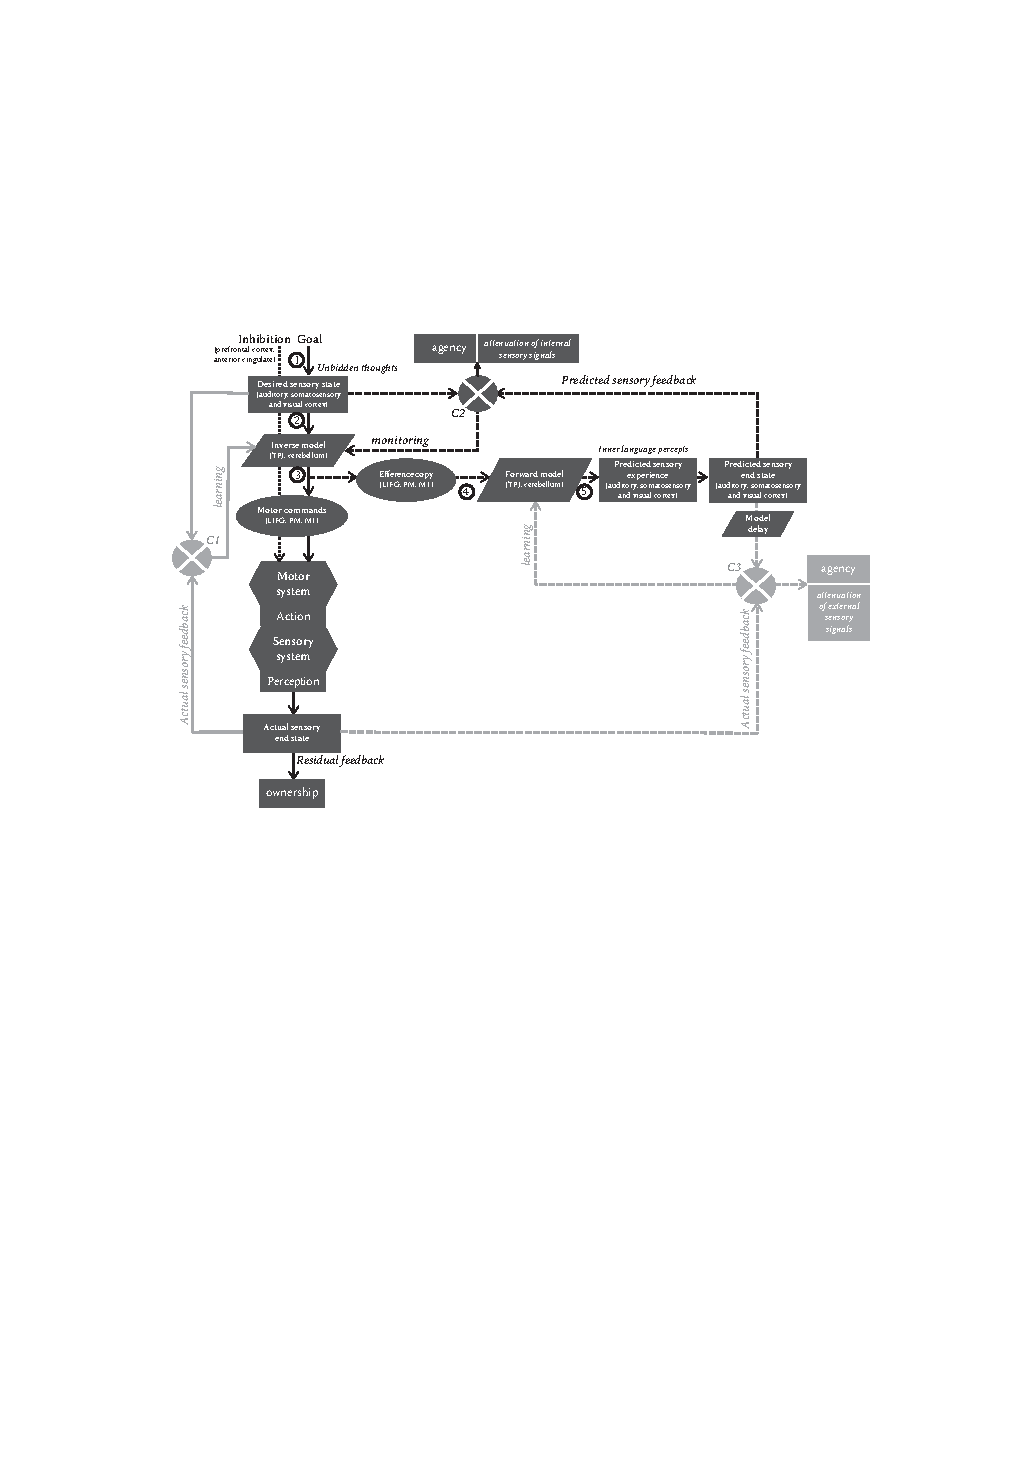
\includegraphics[width=1\linewidth]{assets/loevenbruck1} 

}

\caption{Predictive control account of inner speech production. Figure from L\oe venbruck et al. (2018).}\label{fig:loevenbruck}
\end{figure}

In the previous section, we discussed the relation between the degree of automaticity, the difficulty, and the involvement of the speech motor system during inner speech production. Cohen (\protect\hyperlink{ref-cohen_motor_1986}{1986}) suggested that in difficult situations (e.g., noisy environment, difficult, novel, or degraded verbal material), inner speech percepts may be accentuated to \enquote{attract} more attention as compared to other (non-relevant) stimuli. We can reinterpret these findings in the motor control framework by saying that the involvement of the speech motor system during inner speech (that can be examined via peripheral muscular activation, neuroimagery, or neurostimulation) is a function of the degree of inhibition (the inhibitory signals represented by the vertical dotted lines in Figure \ref{fig:loevenbruck}), with a greater involvement of the speech motor system when inhibition is weaker, and reciprocally, a weaker involvement of the speech motor system when inhibition is stronger. The \enquote{quantitiy and quality} of inhibition (i.e., what proportion of motor commands are inhibited, when, and where) may in turn be a function of contextual and individual characteristics. We might speculate that the reason why inhibition is weaker in demanding situation (e.g., when reading a difficult text or rehearsing novel material) is that understanding more difficult material requires \enquote{clearer} (more vivid) inner speech percepts than understanding known or easy material (the same goes for noisy or degraded material). The exact nature of these inhibitory signals and how the \enquote{amount is inhibition} still need to be examined, however (but see our discussion in section \ref{motor-imagery}).

\begin{figure}

{\centering 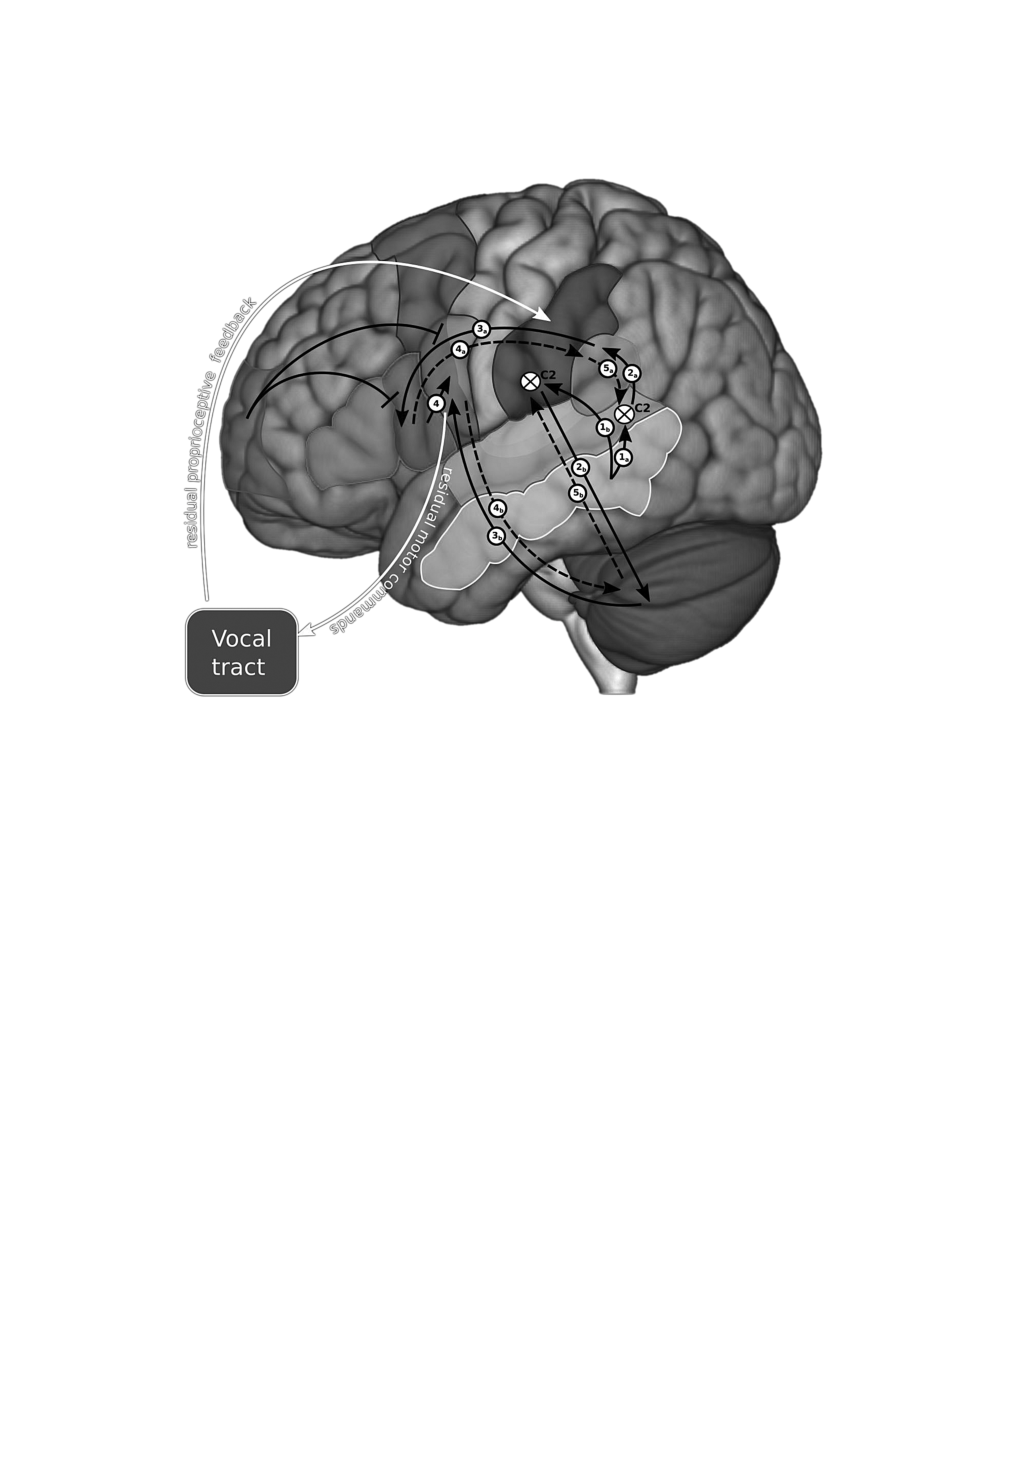
\includegraphics[width=1\linewidth]{assets/loevenbruck2} 

}

\caption{A cerebral landscape of deliberate inner speech production. Figure from L\oe venbruck et al. (2018).}\label{fig:loevenbruck2}
\end{figure}

In addition to explicitly modelling inner speech production in a formal motor control model, Lœvenbruck et al. (\protect\hyperlink{ref-loevenbruck_cognitive_2018}{2018}) proposed a cerebral landscape underlying the production of \emph{deliberate} inner speech (cf.~Figure \ref{fig:loevenbruck2}). This model aims to integrate findings and models from the fields of psycholinguistics and neurolinguistics, as well as neuroanatomical theories of speech production (e.g., Hickok, \protect\hyperlink{ref-hickok_computational_2012}{2012}; Tian \& Poeppel, \protect\hyperlink{ref-tian_effect_2013}{2013}). This model proposes that lemma retrieval is performed by the left middle temporal gyrus (MTG). Then, the lemma is converted to a lexeme in a multisensory format via two routes, the first one providing the auditory representation (a) and the second one providing the somatosensory representation (b). The auditory specification of the desired auditory state then activates the left posterior superior temporal gyrus (pSTG) and the superior temporal sulcus (STS), represented by arrow 1a. In parallel, the somatosensory route activates the anterior supramarginal gyrus (aSMG) and the primary somatosensory cortex (S1), represented by arrow 1b. An inverse model transformation is then performed, again involving two routes. The auditory specification is sent to the temporo-parietal junction (TPJ), represented by arrow 2a. The somatosensory specification is sent to the cerebellum, represented by arrow 2b. Then, motor programmes are specified. The transformed auditory goals are sent from the TPJ to the left IFG and to the left ventral premotor cortex (arrow 3a). The transformed somatosensory goals are sent from the cerebellum to the lower primary motor cortex (M1), represented by arrow 3b. Motor programmes issueds by the left IFG are then sent to M1 (represented by arrow 4), where the two motor programmes computed in the auditory and somatosensory routes are integrated. Importantly, articulation is inhibited via inhibitory signals emitted by the rostral prefrontal cortex (BA 10) and the anterior cingulate gyrus (BA 32) and sent to M1 only, or to both the left IFG and M1. A residual somatosensory feedback may be felt (aSMG and S1), resulting from attenuated motor commands being sent to the motor system. The efference copy mediated by the left IFG is sent to the TPJ (arrow 4a) and is inversed into a predicted auditory signal, activating the pSTG and the STS (arrow 5a). The other copy, in M1, is sent to the cerebellum (arrow 4b) and is inversed into a predicted somatosensory signal, activating th aSMG and S1 (arrow 5b). The comparison between predicted and original desired states (C2) takes place at two sites, in auditory and somatosensory cortices (for more details, see Lœvenbruck et al., \protect\hyperlink{ref-loevenbruck_cognitive_2018}{2018}). It should be noted that this model has been further developed and is presented in working papers or theses (e.g., Grandchamp et al., \protect\hyperlink{ref-grandchamp_neurocognitive_2019}{2019}; Lœvenbruck, \protect\hyperlink{ref-loevenbruck_loquor_2019}{2019}). However, because this work has not been published yet and because of length constraints, we will not discuss the latest version of this model here.

An interesting question related to the application of motor control models to inner speech and imagined actions (but also to executed actions more broadly) is the issue of whether we need both an inverse and a forward model. Pickering \& Clark (\protect\hyperlink{ref-pickering_getting_2014}{2014}) make a distinction between two types of architectures, differing by the place forward models play in these architectures: the auxiliary forward model (AFM) account, according to which forward models are \enquote{special-purpose prediction mechanisms implemented by additional circuitry distinct from core mechanisms of perception and action} and the integrated forward model (IFM) account, according to which \enquote{forward models lie at the heart of all forms of perception and action}. On a similar note, Friston (\protect\hyperlink{ref-friston_what_2011}{2011}) argues for an IFM architecture (instead of conventional motor control schemes) and shows how motor control can be formalised in a Bayesian predictive framework, where optimal control can be seen as an (active) inference. Recently, Wilkinson \& Fernyhough (\protect\hyperlink{ref-wilkinson_auditory_2017}{2017}) similarly suggested to model inner speech production in a \emph{predictive processing framework} (PPF, for an introduction, see for instance Clark, \protect\hyperlink{ref-clark_whatever_2013}{2013}). In this framework, the main task of the brain is thought to be inferring, from incoming signals, what the causes of these signals are. Accordingly, the only information that is passed on up the cortical hierarchy is prediction error, and the hypotheses (about the causes of the percepts) that minimise \emph{prediction error} are selected (or \enquote{inferred}). An interesting consequence of this model applied to motor control is that is does not postulate the existence of motor commands but rather the presence of predictions only, that are fulfilled (or not) by bodily movements (with the aim of minimising prediction error). According to the PPF account of inner speech sketched by Wilkinson \& Fernyhough (\protect\hyperlink{ref-wilkinson_auditory_2017}{2017}), sensory aspects of inner speech (e.g., motor or auditory percepts) may be conceived as predictions in themselves (prediction that have been \enquote{selected} to reduce prediction error), instead of resulting from a stimulus to be monitored.

To understand the appeal of predictive and motor control modelling applied to inner speech and imagined actions, let's consider the analogy between speaking and playing an instrument (e.g., playing the piano). Essentially, learning how to play the piano can be said to consist in learning and coordinating complex and fine-grained motor sequences that produce in turn sensory (e.g., kinesthaetic, auditory, visual) feedback to the producer of the action (the agent). Therefore, it seems that (from a certain level of analysis), the act of speech can be paralleled with the act of playing an instrument in that it consists in the coordination of complex movements that result in some modifications of the environment, that in turn generate sensory feedbacks (e.g., kinesthaetic, auditory) for the agent. Thus, pursuing the analogy, we could argue that the relation between playing an instrument and imagining playing an instrument is similar to the relation between producing speech and imagining speaking (i.e., producing inner speech). This analogy suggests that we might be able to study the development of (pairs of) internal models responsible for the sensory experience accompanying imagined actions in the adult mind (e.g., when an individual is learning either a novel music instrument or a new language with speech sounds that were not present in his native language). By examining the development of novel imagined actions in the adult mind, we might gain new insights about the internalisation of speech during childhood.\footnote{While keeping in mind the obvious limitation that the child mind is not equivalent to the adult mind, nor it is equivalent to a smaller version of the adult mind. However, examining the development of novel imagined actions in adults avoids the contamination of the process of interest (imagined action) by developmental confounds present during childhood.}

This view on the relation between inner speech and overt speech is somehow consistent with Vygotsky's view of inner speech as internalised egocentric speech but it proposes a formal mechanism to explain how overt speech develops into inner speech. More precisely, we might speculate that what is internalised during childhood is an internal model (or a hierarchy of paired internal models). This internalisation is a slow and gradual process and might be similar to the internalisation of other types of motor actions. Considering inner speech as \emph{a} form of motor action brings some interesting insights. Indeed, if speech production can be broadly described as the coordinated sequence of (groups of) muscular movements that result in some predictable sensory consequences (e.g., auditory, visual, kinesthesic or somesthesic feelings), then it can be compared to other actions. In that sense, the process of speech internalisation, as the process of \enquote{internalised walking}, might follow the same general steps. This process can be broadly defined as the learning of the mapping between some muscular commands (or patterns of muscular commands) and the associated sensory consequences. Learning these associations result in the construction of internal models, permitting to predict ongoing actions, but also to simulate these actions in the absence of any overt movement. Therefore, the process of inner speech might be considered under the broad category of imagined actions (motor imagery).

\hypertarget{motor-imagery}{%
\subsection{Explaining the muscular activity observed during inner speech}\label{motor-imagery}}

Motor imagery can be defined as the mental process by which one rehearses a given action, without engaging in the physical movements involved in this particular action. One of the most influential theoretical explanation for this phenomenon is the \emph{motor simulation theory} (MST, Jeannerod, \protect\hyperlink{ref-jeannerod_representing_1994}{1994}, \protect\hyperlink{ref-jeannerod_neural_2001}{2001}, \protect\hyperlink{ref-jeannerod_motor_2006}{2006}). In this framework, the concept of simulation refers to the \enquote{offline rehearsal of neural networks} (Jeannerod, \protect\hyperlink{ref-jeannerod_motor_2006}{2006}) and motor imagery is conceptualised as a simulation of the covert stage of the same executed action (O'Shea \& Moran, \protect\hyperlink{ref-oshea_does_2017}{2017}). The MST shares some similarities with the theories of embodied and grounded cognition (Barsalou, \protect\hyperlink{ref-Barsalou2008}{2008}) in that both allow to account for the phenomenon of motor imagery by appealing to a simulation mechanism. However, the concept of simulation in grounded theories is assumed to be multi-modal (not just motoric) and to operate in order to achieve a particular abstract knowledge (O'Shea \& Moran, \protect\hyperlink{ref-oshea_does_2017}{2017}), which is not the concern of the MST\footnote{We should also make a distinction between \emph{embodiment of content}, which concerns the conceptual content of language, and \emph{embodiment of form}, which concerns \enquote{the vehicle of thought}, that is, proper speech production (Pickering \& Garrod, \protect\hyperlink{ref-pickering_integrated_2013}{2013}).}. As highlighted by O'Shea \& Moran (\protect\hyperlink{ref-oshea_does_2017}{2017}), the MST contains the three following postulates at its core: i) there exists a continuum between the covert (the mental representation) and the overt execution of an action, ii) action representations can operate off-line, via a \emph{simulation} mechanism, and iii) covert actions rely on the same set of mechanisms as the overt actions they simulate, except that execution is inhibited. The MST is supported by a wealth a findings, going from mental chronometry studies showing that the time taken to perform an action is often found to be similar to the time needed to imagine the corresponding action (but see Glover \& Baran, \protect\hyperlink{ref-glover_motor-cognitive_2017}{2017}, for a review of chronometric findings and for an alternative conceptualisation of motor imagery)\footnote{Although not always. As previously discussed in section \ref{inner-speech-history}, Guillot et al. (\protect\hyperlink{ref-guillot_understanding_2012}{2012}\protect\hyperlink{ref-guillot_understanding_2012}{b}) reviewed chronometric findings related to motor imagery and listed the several factors that may affect the temporal equivalence between executed and imagined actions.}, to neuroimaging and neurostimulation studies showing that both motor imagery and overt actions tend to recruit similar frontal, parietal and sub-cortical regions (e.g., Hétu et al., \protect\hyperlink{ref-hetu_neural_2013}{2013}; Jeannerod, \protect\hyperlink{ref-jeannerod_neural_2001}{2001}). The involvement of the motor system during motor imagery is also supported by repeated observations of autonomic responses, increased corticospinal excitability, as well as peripheral muscular activity during motor imagery (for an overview, see Collet \& Guillot, \protect\hyperlink{ref-collet_autonomic_2010}{2010}; Jeannerod, \protect\hyperlink{ref-jeannerod_motor_2006}{2006}; Stinear, \protect\hyperlink{ref-stinear_corticospinal_2010}{2010}).

Motor imagery has consistently been defined as the mental rehearsal of a motor action without any overt movement. One consequence of this claim is that, in order to prevent execution, the neural commands for muscular contractions should be blocked at some level of the motor system by active inhibitory mechanisms (for a review, see Guillot et al., \protect\hyperlink{ref-guillot_imagining_2012}{2012}\protect\hyperlink{ref-guillot_imagining_2012}{a}). Despite these inhibitory mechanisms, there is now abundant evidence for peripheral muscular activation during motor imagery (for a review, see Guillot \& Collet, \protect\hyperlink{ref-guillot_contribution_2005}{2005}; Guillot et al., \protect\hyperlink{ref-guillot_imagining_2012}{2012}\protect\hyperlink{ref-guillot_imagining_2012}{a}). As suggested by Jeannerod (\protect\hyperlink{ref-jeannerod_representing_1994}{1994}), the incomplete inhibition of the motor commands would provide a valid explanation to account for the peripheral muscular activity observed during motor imagery. Consistent with this assumption, Schwoebel, Boronat, \& Branch Coslett (\protect\hyperlink{ref-schwoebel_man_2002}{2002}) showed that a brain-damaged patient failed to inhibit the motor consequences of motor imagery, and thus fully \enquote{executed the imagined action}, hence highlighting uninhibited movements during mental rehearsal.\footnote{However, it should be noted that Schwoebel et al. (\protect\hyperlink{ref-schwoebel_man_2002}{2002}) reported no difficulty for this patient to read silently.} This idea has also been corroborated by studies of changes in the excitability of the motor pathways during motor imagery tasks. Bonnet, Decety, Jeannerod, \& Requin (\protect\hyperlink{ref-bonnet_mental_1997}{1997}) measured spinal reflexes while participants were instructed to either press a pedal with the foot or to simulate the same action mentally. They observed that both H-reflexes and T-reflexes increased during motor imagery, and that these increases correlated with the force of the simulated pressure. Using transcranial magnetic stimulation and motor evoked potentials (MEPs), several investigators observed muscle-specific increases of MEPs during various motor imagery tasks, whereas no such increase could be observed in antagonist muscles (e.g., Fadiga et al., \protect\hyperlink{ref-fadiga_corticospinal_1999}{1999}; Rossini, \protect\hyperlink{ref-rossini_corticospinal_1999}{1999}).

However, although there are many observations showing a peripheral muscular activity during motor imagery, there are also many studies failing to do so, or reporting surprisingly high levels of inter-subject variability, with some participants showing no muscular activity at all (for a review, see Guillot, Lebon, \& Collet, \protect\hyperlink{ref-guillot_electromyographic_2010}{2010}). Two main explanations have been advanced to resolve these discrepancies. First, the electromyographic activity recorded during motor imagery could be moderated by the perspective taken in motor imagery.\footnote{We usually make a distinction between a first-person perspective or \emph{internal imagery} (i.e., imagining an action as we would execute it) and a third-person perspective or \emph{external imagery} (i.e., imagining an action as an observer of this action), that seem to involve different neural and cognitive processes.} Indeed, it has been shown that a first-person perspective generally results in greater EMG activity than motor imagery in a third-person perspective (Hale, \protect\hyperlink{ref-hale_effects_1982}{1982}; Harris \& Robinson, \protect\hyperlink{ref-harris_effects_1986}{1986}). Second, some authors postulated that the intensity of the EMG activity recorded during motor imagery might be related to the individual ability to form an accurate mental representation of the motor skill (i.e., the vividness of the mental image). However, after reviewing the available evidence, Guillot et al. (\protect\hyperlink{ref-guillot_brain_2009}{2009}) concluded that this is unlikely to be the case. Alternatively, discrepancies in experimental design and methodological choices (e.g., use of intramuscular versus surface electromyography) could also explain these contradictory results (Guillot et al., \protect\hyperlink{ref-guillot_electromyographic_2010}{2010}).

\vspace{2mm}

\begin{mybox}[label = inhibition]{The motor inhibition problem}

The "problem of inhibition" can be summarised as follows (from Jeannerod, 2001, page S106): how come that covert actions, in spite of activation of the motor system, do not result in muscular activity and overt movements?\\

An attractive answer to that question is that imagined actions can be considered as inhibited actions. The neural generators of these inhibitory signals, however, have not yet been clearly identified in the motor imagery literature. As reviewed in Guillot et al. (2012a), previous research has suggested at least three (non-exclusive) potential inhibitory mechanisms that might operate during motor imagery:

\begin{itemize}

\item First, motor inhibition might be \textit{integrated} within the construction of the mental representation (i.e., imagination would simply be a weaker form of execution), hence only \textit{subthreshold} (i.e., insufficient to induce motoneurons excitation) motor commands are sent to the effectors to prevent movement execution.

\item Second, inhibitory mechanisms may be triggered in conjunction with motor commands (e.g., Jeannerod, 2006): inhibitory cerebral regions might progressively weaken the motor commands during the time course of motor imagery, so that only a \textit{residual} activity is sent.

\item Third, inhibitory mechanisms might be located downstream of the motor cortex, possibly at the spinal or brainsteam level (e.g., Jeannerod, 2001; 2006). Lotze \& Halsband (2006) also suggested that the posterior cerebellum might play a crucial role in inhibiting the motor commands.

\end{itemize}

Therefore, motor commands inhibition might intervene in three non-exclusive ways during motor imagery. However, the exact contribution of each route still needs to be examined.

\end{mybox}

In order to investigate the inhibitory mechanisms involved during motor imagery, Rieger, Dahm, \& Koch (\protect\hyperlink{ref-rieger_inhibition_2017}{2017}) extended the logic of task switching paradigms and developed a novel \emph{action mode} (imagery vs.~execution) switching paradigm. In these procedures, performance in the current trial is analysed depending on the condition of the previous trial, assuming that execution or inhibition in the previous trial persists to a certain degree. Put simply, the main idea is that inhibition during motor imagery should leave after-effects by increasing activation thresholds, then affecting the performance of subsequently executed (or imagined) movements. In analysing sequential effects, Rieger et al. (\protect\hyperlink{ref-rieger_inhibition_2017}{2017}) observed shorter movement times when motor execution (ME) preceded motor imagery (MI) than when motor imagery preceded motor execution, corroborating the idea of a global inhibition (i.e., the second option from Box \ref{inhibition}) mechanism taking place during motor imagery. In addition, they observed hand repetition costs (i.e., movement times were longer when the task had to be performed with the same hand than with the other hand in motor imagery trials), suggesting that effector-specific inhibitory mechanisms may also taking place during motor imagery (corroborating the third option discussed in Box \ref{inhibition}). However, as highlighted by O'Shea \& Moran (\protect\hyperlink{ref-oshea_go_2018}{2018}), global inhibitory mechanisms may also induces longer movements times in MI-ME sequences than in ME-ME sequences, but this effect was not observed in Rieger et al. (\protect\hyperlink{ref-rieger_inhibition_2017}{2017}). To push forward this investigation, O'Shea \& Moran (\protect\hyperlink{ref-oshea_go_2018}{2018}) used pupillometry to examine the degree of attentional effort involved in the execution or the inhibition of a motor response during both motor imagery and motor execution in a Go/NoGo procedure, embedded in a modified task-switching paradigm. They observed that the amount of attentional effort (assessed via pupillometry) varied according to the type of block (i.e., pure vs.~mixed), suggesting that different inhibitory mechanisms (or \enquote{routes}) may underlie inhibition during motor imagery. For instance, it may be that inhibition during motor imagery is programmed in a pre-emptive way when the participants know that the next block will be uniquely composed of motor imagery trials or in a more active (and more effort-costly) way in mixed blocks. Therefore, different inhibitory mechanisms (e.g., proactive vs.~reactive, global vs.~selective) may also vary according to the task characteristics (for a more detailed discussion of these findings, see also O'Shea, \protect\hyperlink{ref-oshea_investigation_2017}{2017}). Although these studies are among the first to investigate these issues, they show that it is possible to use a combination of cognitive and psychophysiological tasks to assess the inhibitory mechanisms involved during motor imagery.

To sum up this section, the available neural and psychophysiological evidence suggests that inner speech and imagined actions may result from internal simulation (or emulation) of the corresponding executed action. This appealing idea however presupposes that the motor commands emitted during inner speech (from which result the sensory percepts of inner speech such as the inner voice) are somehow completely or partially inhibited in order to prevent execution. We discussed several explanations with regards to the source of these inhibitory signals (that remains to be tested in the case of inner speech). Interestingly, these questions echo our previous discussion of the centralism versus peripheralism debate (cf.~Box \ref{centralism}). Recent theoretical frameworks of inner speech and motor imagery (e.g., motor control models, simulation and emulation theories) are \emph{centralist} theories of motor cognition. Indeed, in these frameworks, the peripheral muscular activity observed during imagined action is conceived as a consequence of (a partial inhibition) these actions, rather than a \emph{necessary} condition for imagining actions (including speech). This idea was well summarised by Jeannerod (\protect\hyperlink{ref-jeannerod_motor_2006}{2006}), discussing the motor inhibition problem and the case of subvocal (inner) speech:

\begin{quote}
\enquote{Subvocal speech was first interpreted as a source of peripheral kinesthetic information which, when projected to central nervous structures, generated auditory images of the corresponding words. The same interpretation was given to the low intensity EMG recorded during mental motor imagery of limb actions, which was thought to be the origin of the feelings experienced by the subject during mental rehearsal (Jacobson, 1930), or to the eye movements recorded during mental visual imagery (e.g., Brandt and Stark, 1997). However, this interpretation of mental processes as consequences of peripheral feedback is now disproved by recent experiments showing complete absence of muscular activity in many subjects during motor imagery. When present, this activity is rather assumed to be a consequence of incomplete inhibition of motor output during mental states involving motor simulation. This same interpretation might also hold for inner speech.} (p.153)
\end{quote}

Therefore, although the precise neural generators of these inhibitory signals remain to be examined, the peripheral muscular activation observed during inner speech may be resulting from an incomplete inhibition of motor commands. Moreover, we may speculate that some forms of inner speech may or may not be accompanied by peripheral muscular activations in the speech muscles, depending on the degree (the amount) of inhibition.

\hypertarget{summary-problematic-and-directions}{%
\section{Summary, problematic and directions}\label{summary-problematic-and-directions}}

We reviewed the main theoretical positions about rumination, the different ways it has been assessed (either as a trait or as a state) and discussed the sensory properties of ruminative thoughts. Acknowledging the predominantly verbal character of rumination, we suggested that it might be considered as a form of inner speech. In order to understand the repercussions of this assumption with regards to the study of rumination, we presented a brief historical review of inner speech research from 1850 to present days. This review lead us to a presentation of the main contemporary theoretical views on inner speech and to the suggestion that inner speech may be conceived as a form of motor imagery and that it could be understood and modelled in a motor control framework. We then briefly discussed findings from the the field of motor cognition and the study of motor imagery to take a new perspective on the findings previously discussed about the involvement of the speech motor system during inner speech production. In consideration of this discussion, the main goals of the present work are i) to refine the description of inner speech and the involvement of the speech motor system during its production by studying a particular form of inner speech (i.e., rumination) and ii) to shed a new light on rumination by studying it as a form of inner speech, with the potential outcome of providing psychophysiological (electromyographic) markers of (induced) rumination. Before turning to a presentation of this experimental work (where each study is presented as a standalone empirical article, cf.~Chapters \ref{chap3} to \ref{chap7}), in the next chapter, we briefly introduce some key elements and technical details with regards to the methods we used in this work.

\hypertarget{chap2}{%
\chapter{Methodological framework}\label{chap2}}

\epigraph{"[...] we have been brainwashed by Fisherian statistics into thinking that refutation of $H_{0}$ is a powerful way of testing substantive theories"}{Meehl, P. (1986)}

\initial{I}n this chapter we briefly introduce some of the key concepts related to the methods we used in our work. More precisely, we cover the technical concepts related to speech production mechanisms, to electromyography and to our statistical approach. Finally, we give an overview of the following chapters.

\hypertarget{biomechanical-aspects-of-speech-production}{%
\section{Biomechanical aspects of speech production}\label{biomechanical-aspects-of-speech-production}}

\hypertarget{vocal-apparatus}{%
\subsection{Vocal apparatus}\label{vocal-apparatus}}

Speech production requires the involvement of more than 100 muscles in the face, the neck and the chest (Simonyan \& Horwitz, \protect\hyperlink{ref-simonyan_laryngeal_2011}{2011}). The activity of these muscles is coordinated to produce an air flow moving from the lungs to the oral and nasal cavities, via the trachea, the larynx and the pharynx (see Figure \ref{fig:vocal}). Broadly speaking, speech production can be said to consist essentially in i) \emph{phonation}, which refers to the manipulation of the air flow and to the vibration of the vocal folds and ii) \emph{articulation}, which refers to movements of the \emph{articulators}. The action of the \emph{articulators} (e.g., lips, tongue) is to shape the oral and nasal cavities, resulting in modifications of the sound waves and in the production of different vowels.

\begin{figure}

{\centering 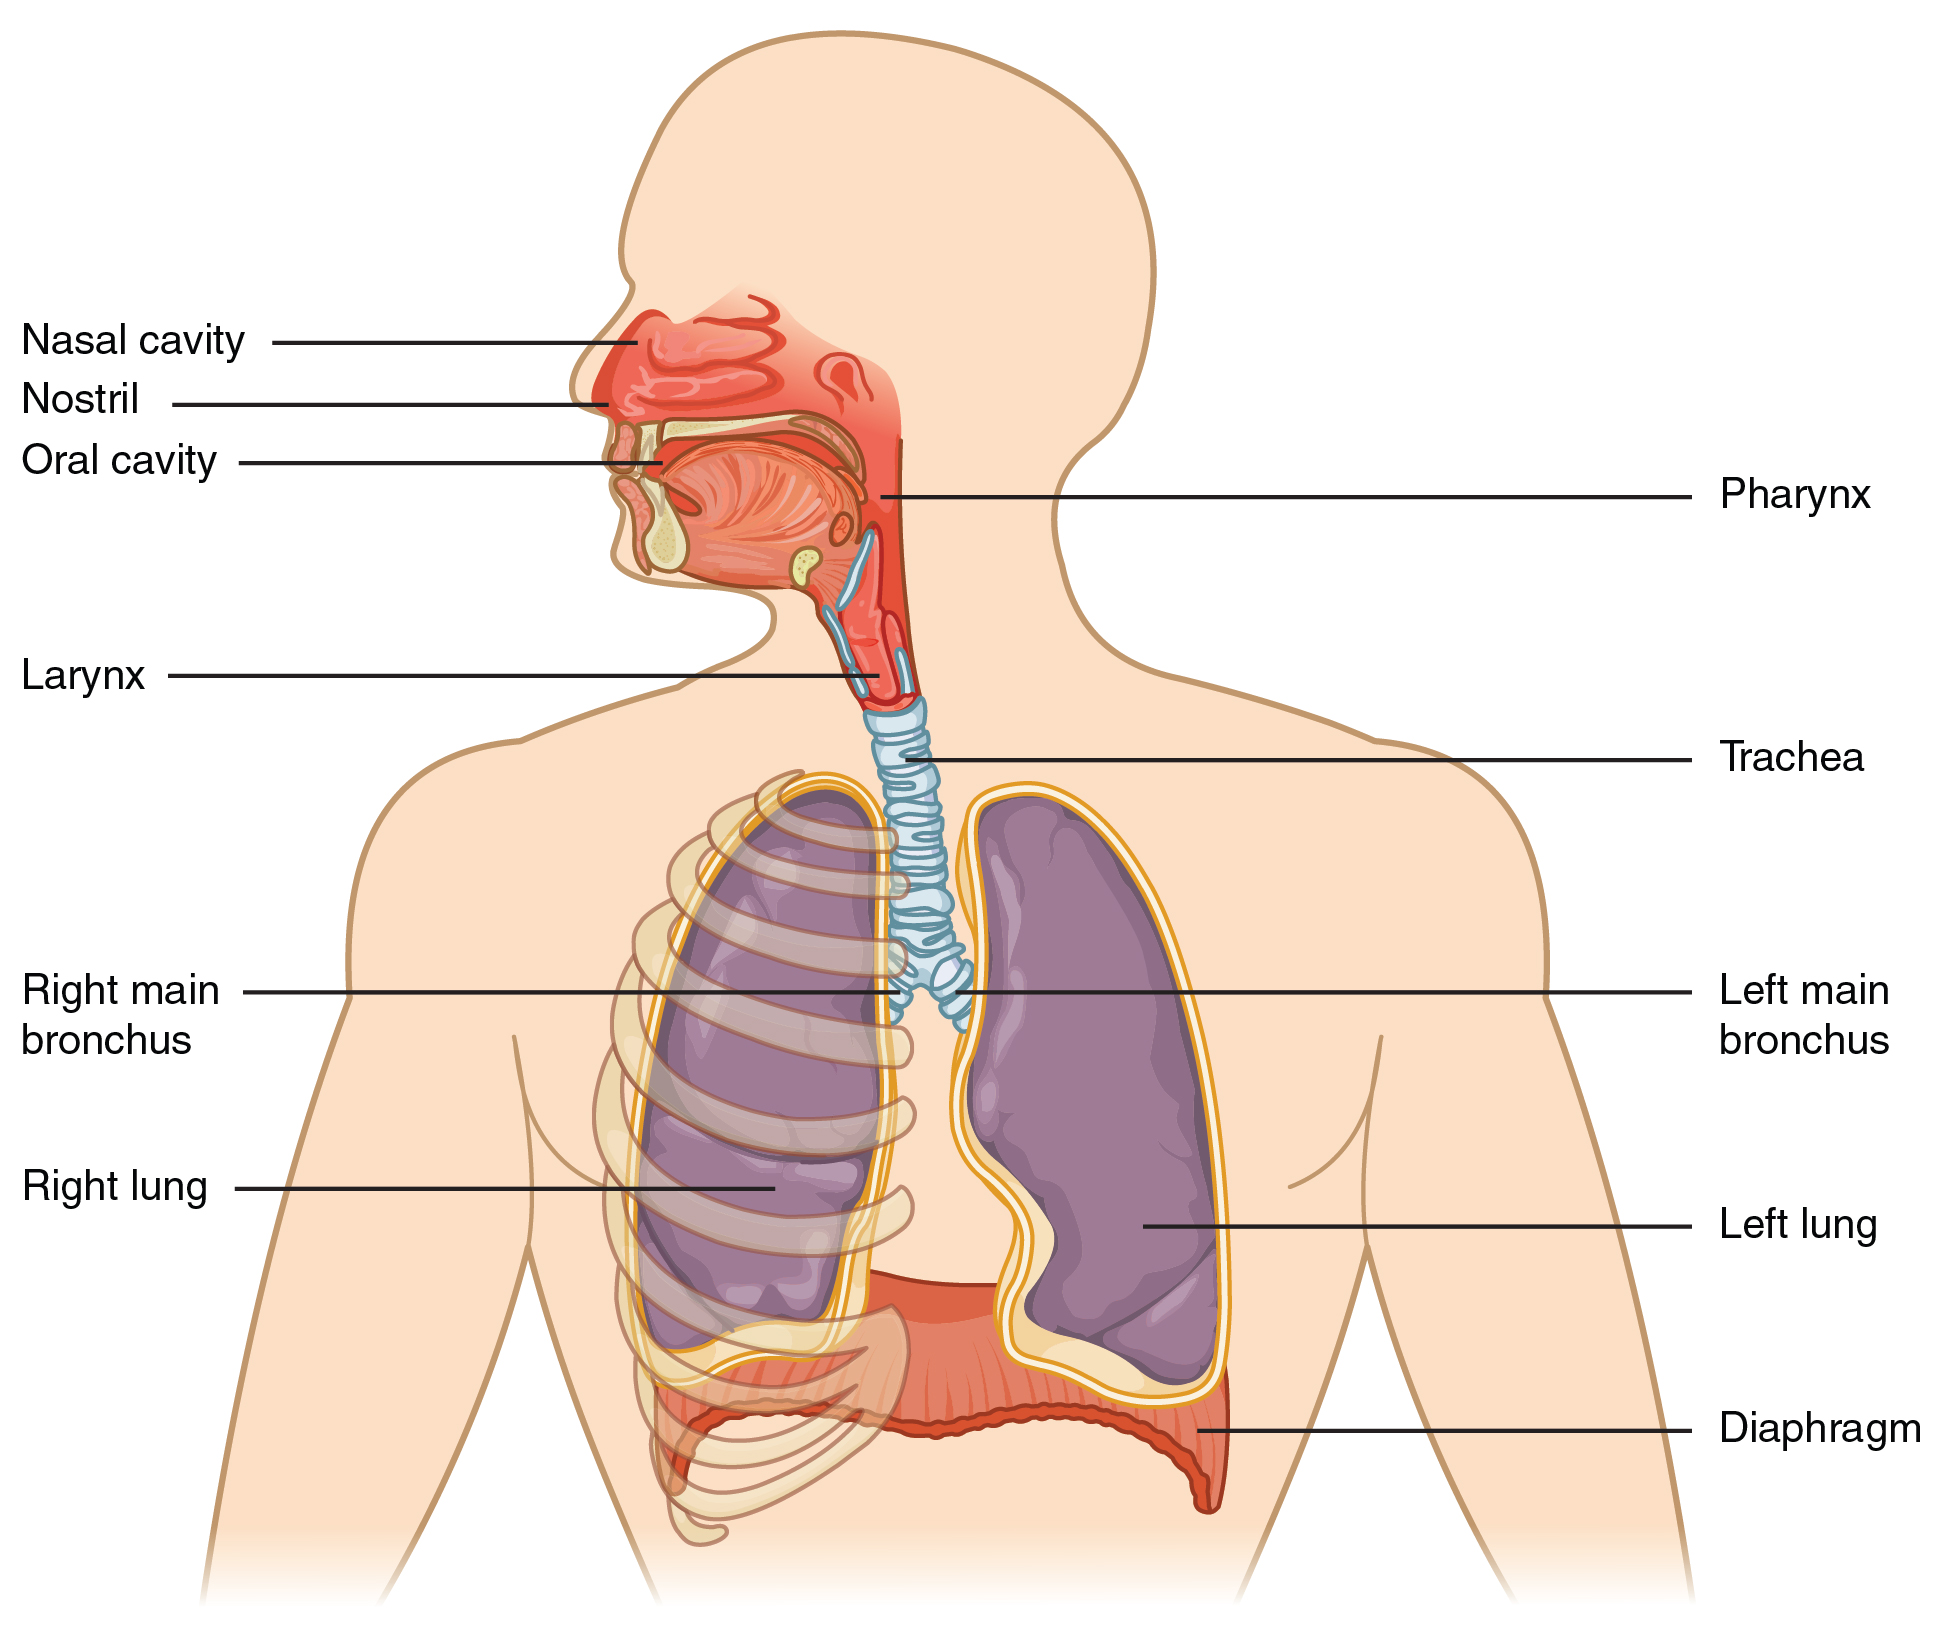
\includegraphics[width=0.5\linewidth]{assets/vocal} 

}

\caption{Human respiratory and phonatory system. Figure from the OpenStax \textit{Anatomy and Physiology} Textbook. Download for free at \url{https://cnx.org/contents/14fb4ad7-39a1-4eee-ab6e-3ef2482e3e22@15.1}.}\label{fig:vocal}
\end{figure}

The characteristics of the vocal folds (e.g., their length or thickness) influence what is known as the \emph{fundamental frequency} (or F0) of the speech signal, which in turn determines the perceived pitch of the voice. The speech signal can be further decomposed in \emph{resonant frequencies} or \emph{formants}. Interestingly, we can relate changes in the state of the articulatory system with changes in the formant (and especially the F1-F2) space (see Figure \ref{fig:ipa}). Indeed, the frequency of the first formant (F1) is mostly determined by the height of the tongue body whereas the frequency of the second formant (F2) is mostly determined by the frontness/backness of the tongue body. For instance, when producing the /u/ vowel, the tongue is positioned at the top and in the back of the oral cavity (and the lips are rounded). However, when producing the /a/ vowel, the tongue is positioned at the bottom of the oral activity (and the lips are widely opened).

\begin{figure}

{\centering 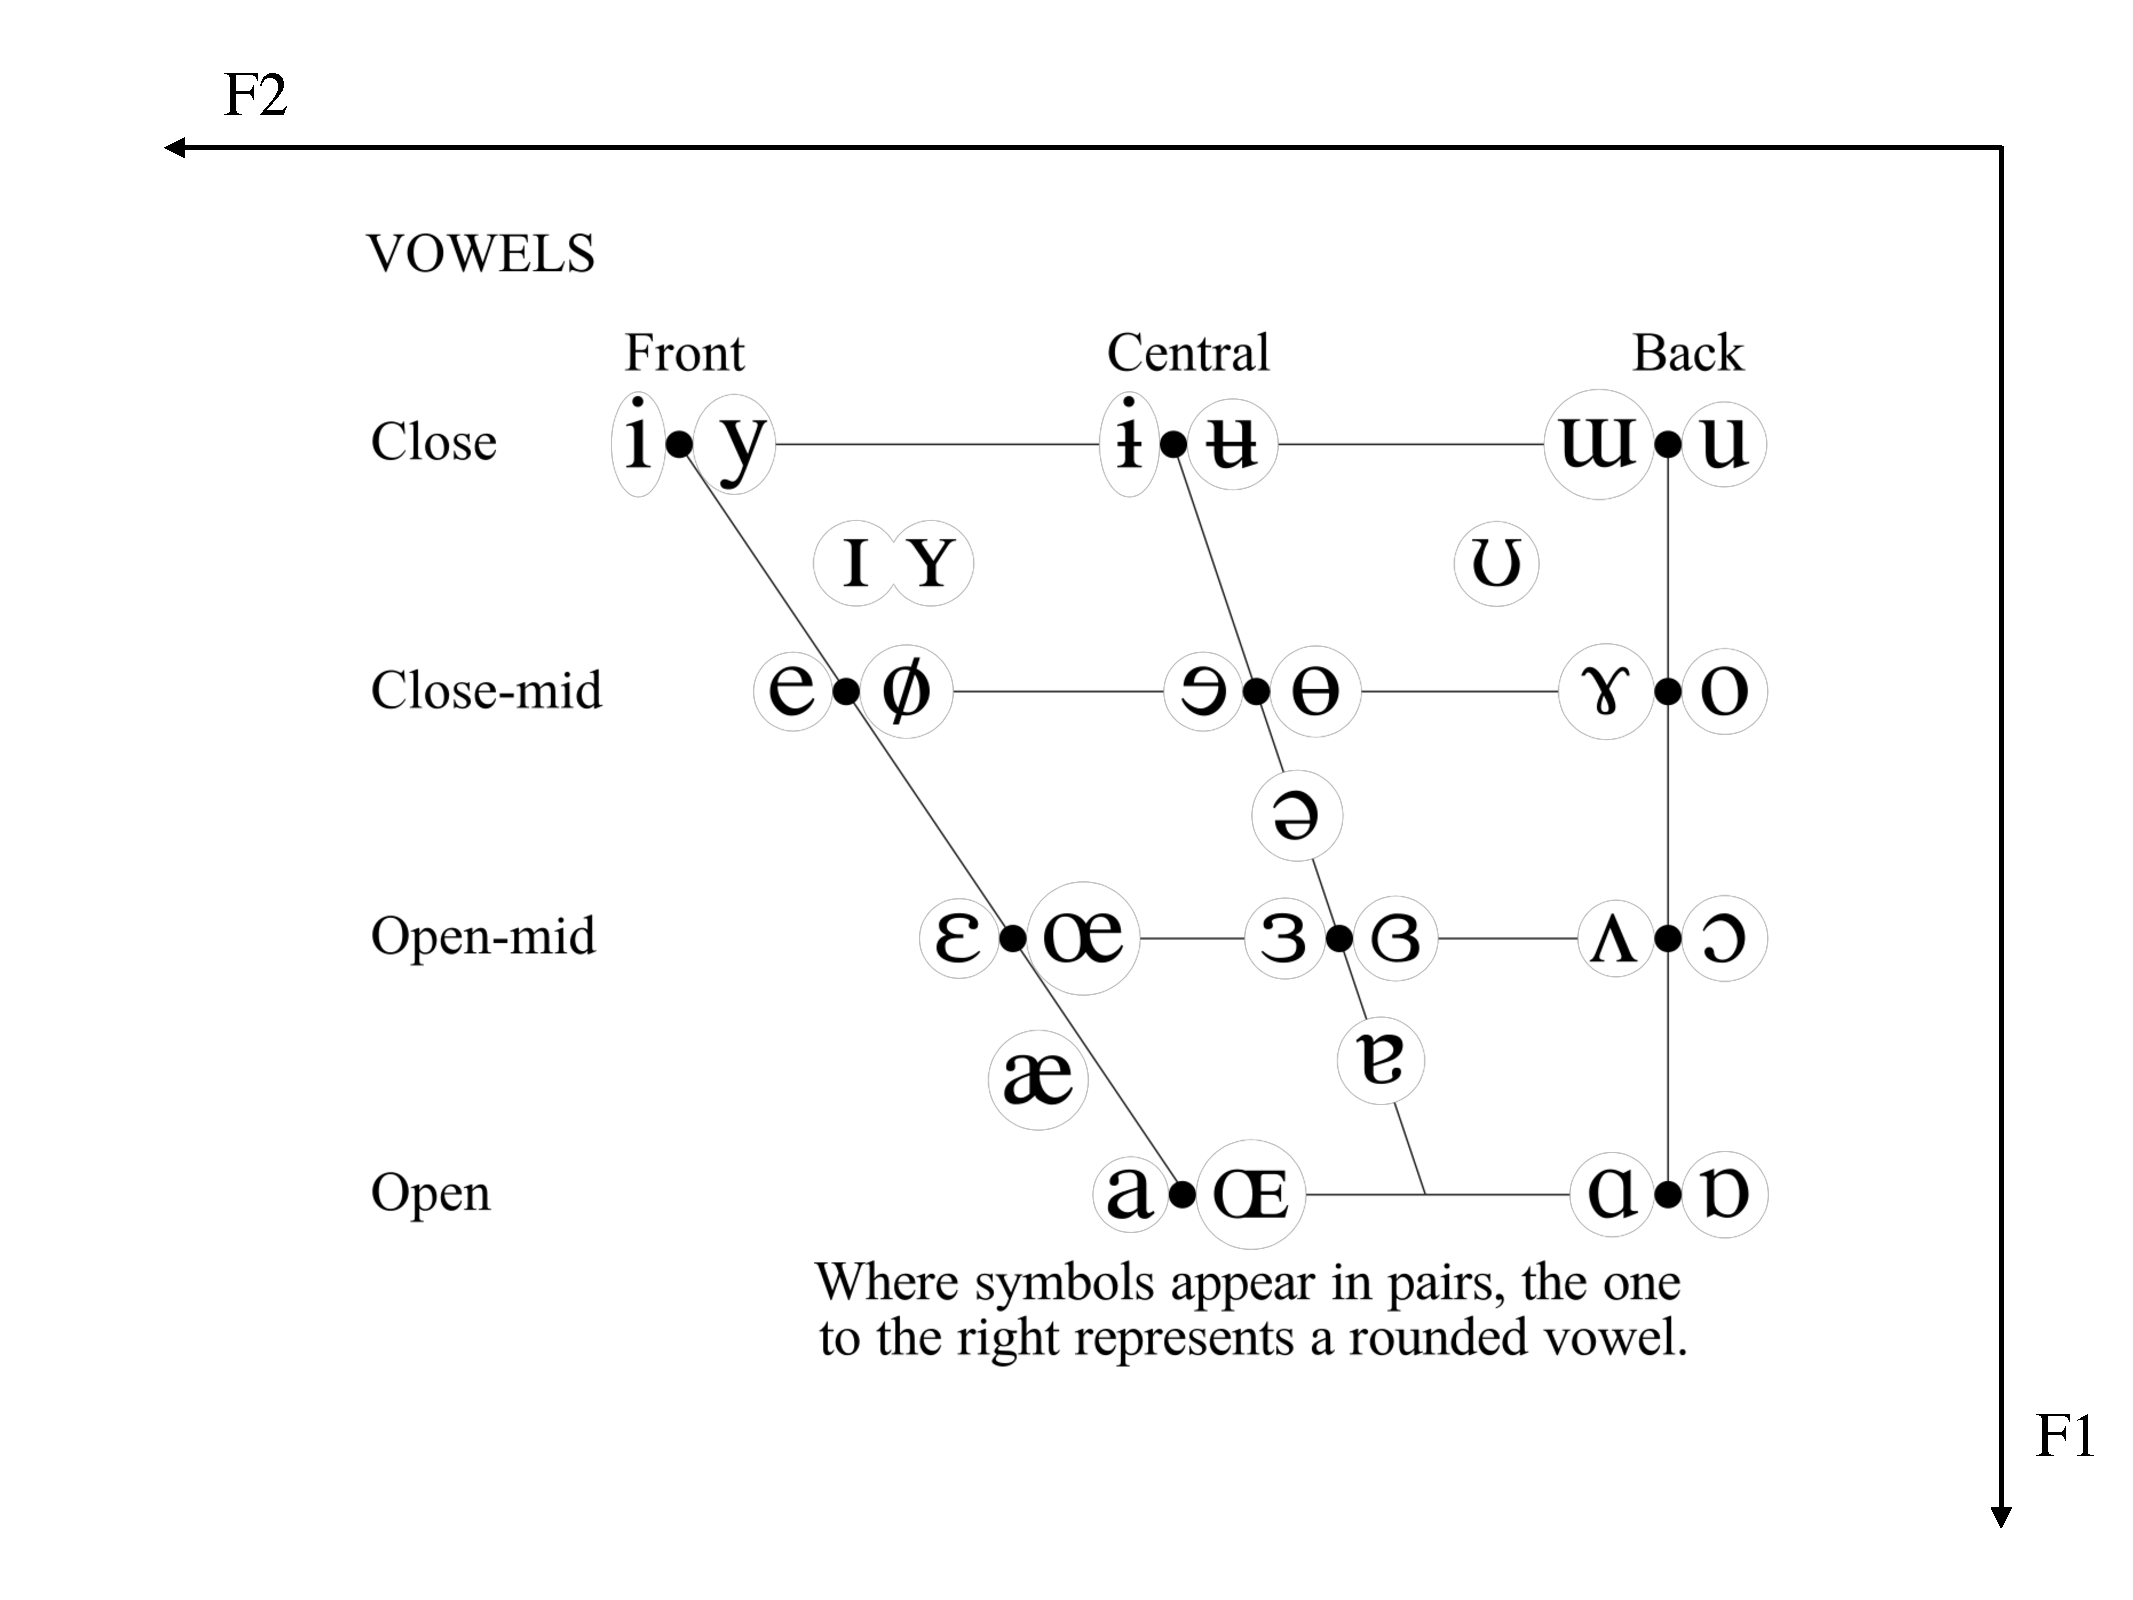
\includegraphics[width=0.75\linewidth]{assets/vowels} 

}

\caption{Illustration of the vocalic 'quadrilateral' and the relation between vowels and formants (F1 and F2). Figure adapted from the International Phonetic Association (2015) - IPA Chart, available under a Creative Commons Attribution-Sharealike 3.0 Unported License.}\label{fig:ipa}
\end{figure}

In brief, modifications in the shape of the \emph{vocal tract} result in the production of different vowels. Changes in the configuration of articulators such as the lips or the tongue may also produce consonants. Consonants are produced by applying some form of restriction to (or by closing) the vocal tract to constraint the air flow. We usually classify consonants according to \emph{where} (the \emph{place of articulation}) and \emph{how} (the \emph{manner of articulation}) this restriction takes place (see Figure \ref{fig:consonants}). For instance, consonants such as /p/ or /b/ are produced by putting the lips together and are therefore known as \emph{bilabial} consonants.

\begin{figure}

{\centering 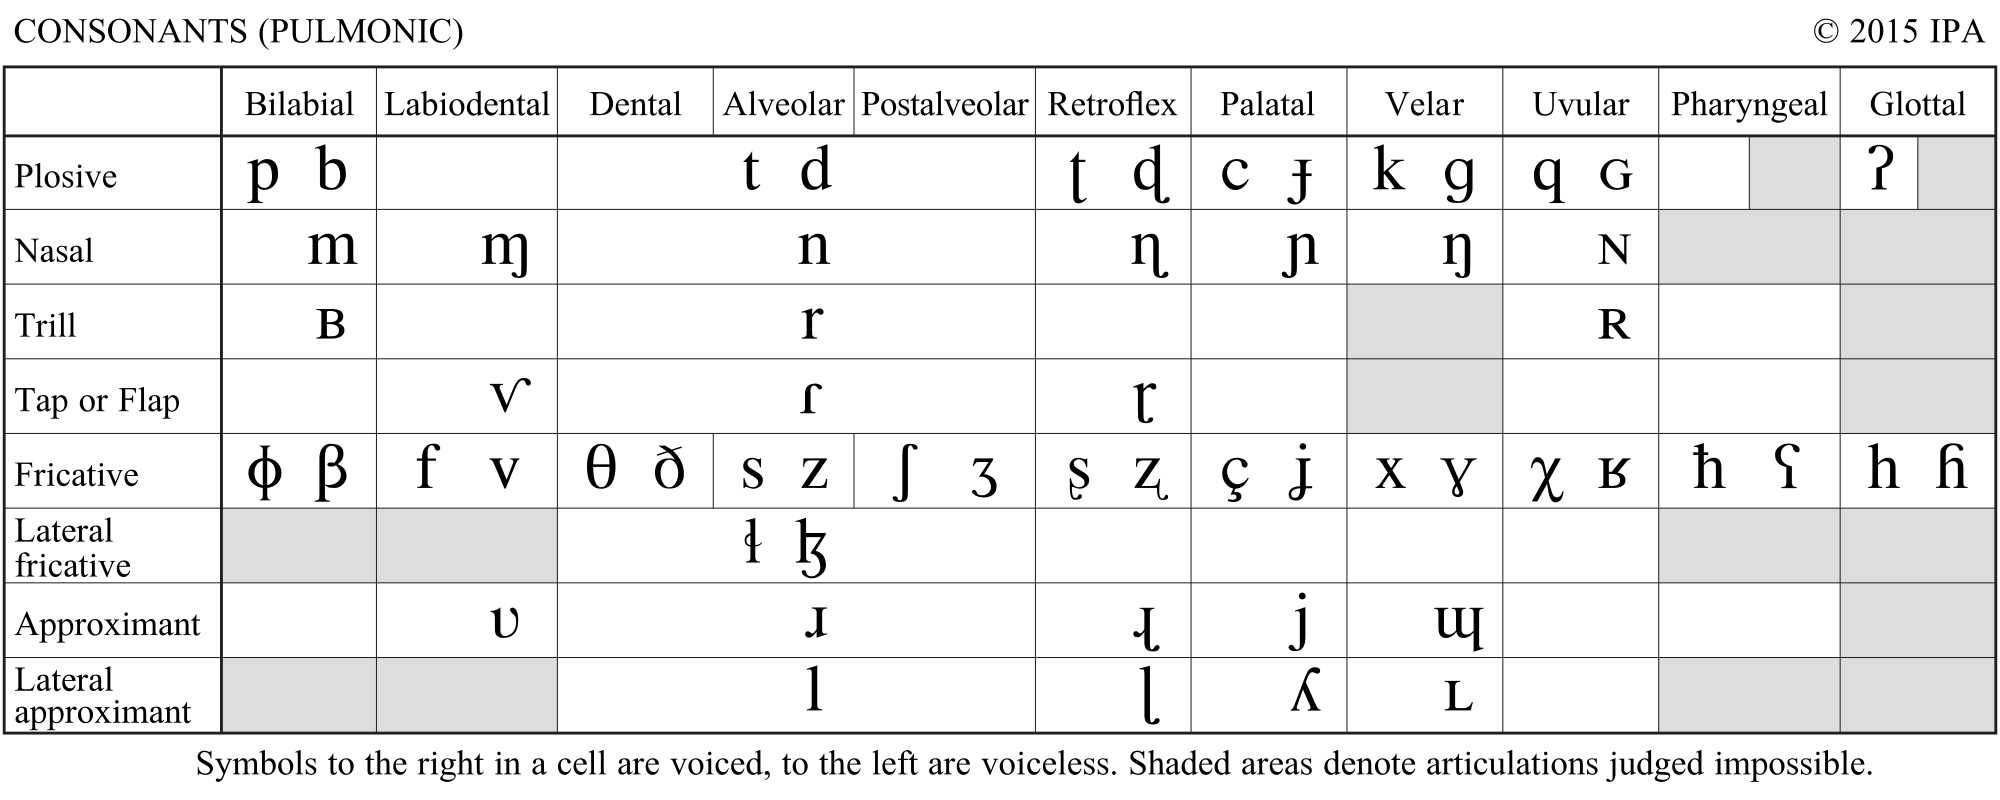
\includegraphics[width=1\linewidth]{assets/consonants} 

}

\caption{Table of consonants according to the manner (in rows) and place (in columns) of articulation. Figure from the International Phonetic Association (2015) - IPA Chart, available under a Creative Commons Attribution-Sharealike 3.0 Unported License.}\label{fig:consonants}
\end{figure}

To sum up, besides from being an essential communication tool for humans, speech production is also a complex motor action, involving the fine-grained coordination of numerous muscles. In the next section, we discuss in more details the specific facial muscles that were of interest in the present work.

\hypertarget{orofacial-speech-muscles}{%
\subsection{Orofacial speech muscles}\label{orofacial-speech-muscles}}

In our work, we were especially interested in the activity of some of the orofacial muscles (i.e., the muscles situated around the mouth). More precisely, we studied the activity of the \emph{orbicularis oris inferior} (OOI), the \emph{orbicularis oris superior} (OOS), and the \emph{zygomaticus major} (ZYG) muscles (cf.~Figure \ref{fig:facial}). Contrary to what was assumed until recently, the \emph{orblicularis oris} muscle is not a sphincter muscle but is instead a complex of several distinct muscles that interlace in a way that gives the \emph{orbicularis oris} complex its circular aspect. Among these muscles, the OOS and the OOI are placed above and below (respectively) the mouth and are responsible for rounding or protruding the lips. More precisely, the OOS is responsible for lowering the upper lip whereas the OOI is responsible for elevating the lower lip. The ZYG muscle has its origin on the zygomatic bone and inserts at the labial commissure (the angle of the mouth) where it meets with fibers of the \emph{levator anguli oris} and \emph{orbicularis oris} muscles. Together with the \emph{levator anguli oris}, it serves to move the labial commissure upwards and laterally, and is involved in laughing and more generally in pleasant reactions and positive emotions. It is also involved in speech production, especially during the production of \emph{spread} sounds, that is, sounds that require a wide aperture of the mouth (e.g., /i/).

\begin{figure}

{\centering 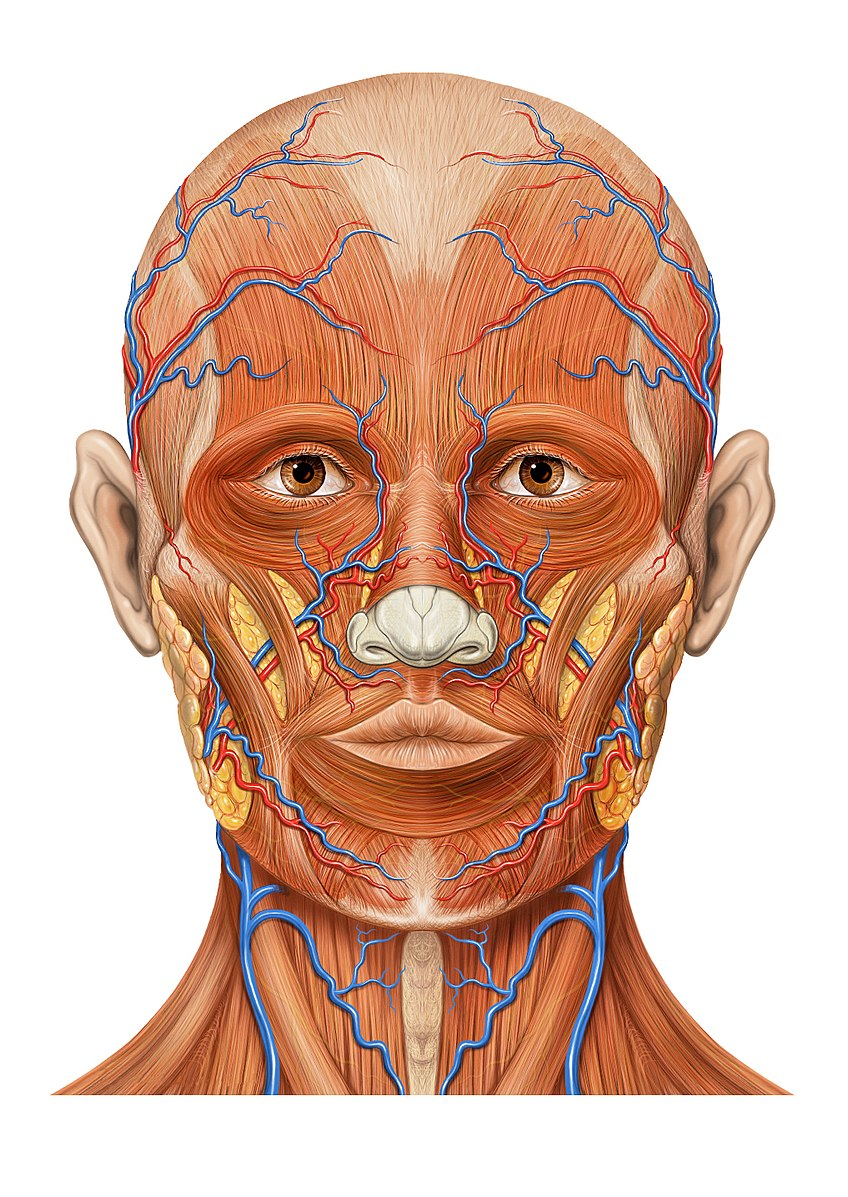
\includegraphics[width=0.75\linewidth]{assets/facial_muscles} 

}

\caption{Illustration of the main facial muscles of interest in the present work. Figure adapted from Patrick J. Lynch, medical illustrator, http://patricklynch.net.}\label{fig:facial}
\end{figure}

For sensors placement, we followed guidelines and recommendations from Fridlund \& Cacioppo (\protect\hyperlink{ref-fridlund_guidelines_1986}{1986}). In addition to speech-related orofacial muscles, we also routinely recorded the activity of other facial muscles such as the \emph{frontalis} muscle (FRO) in Chapter \ref{chap3}, \ref{chap4}, \ref{chap5}, and the \emph{corrugator supercilii} muscle (COR) in Chapter \ref{chap5}. The activity of these muscles was monitored to control for non speech-related facial muscular activity (as recommended by Garrity, \protect\hyperlink{ref-garrity_electromyography_1977}{1977}).

There are several ways to probe the involvement of specific articulators in a given speech production task. For instance, it is possible to selectively interfere with the activity of some articulators (or groups of articulators) to demonstrate their necessary involvement in this particular task. It is also possible to record the activity of facial muscles peripherally using surface electromyography, without interfering with (or with minimal interference to) the natural course of the speech production process. In the next section, we briefly introduce some core concepts of electromyography.

\hypertarget{a-brief-introduction-to-electromyography}{%
\section{A brief introduction to electromyography}\label{a-brief-introduction-to-electromyography}}

Technically speaking, electromyography (EMG) is a technique concerned with the recording and analysis of myoelectric signals (i.e., signals resulting from physiological variations in the state of muscle fibers membranes). Broadly speaking, EMG is a measure of the electrical activity generated during muscle contraction. It is used both as a basic tool in (for instance) biomechanical and psychophysiology research and as an evaluation tool in applied research (e.g., physiotherapy, rehabilitation, human-computer interfaces). To facilitate the interpretation of the EMG signal, it is useful to briefly detail the meaning of its physiological components.

\hypertarget{nature-of-the-emg-signal}{%
\subsection{Nature of the EMG signal}\label{nature-of-the-emg-signal}}

\hypertarget{muscular-anatomy-and-physiology}{%
\subsubsection{Muscular anatomy and physiology}\label{muscular-anatomy-and-physiology}}

A muscle is a collection of fibers that can vary in length, orientation, diameter, and architectural characteristics. For instance, deeper muscle fibers are usually composed of a greater proportion of slow-twitch fibers (type I muscle fibers) whereas more superficial muscle fibers comprise a greater proportion of larger and fast-twitch fibers (type II muscles fibers, Kamen \& Gabriel, \protect\hyperlink{ref-kamen_essentials_2010}{2010}). On the basis of their structure and contractile properties, we can identify three types of muscle tissues: i) the \emph{skeletal muscles} are attached to bones, their function is to produce voluntary movements and to protect the organs, ii) the \emph{cardiac muscles}, whose function is to pump blood and iii) the \emph{smooth muscles}, involved in involuntary movements (e.g., respiration, moving food).

The contraction of the skeletal muscles is initiated by electrical impulses that propagate from the central nervous system to the muscle via the \(\alpha\)-motoneurons. Interestingly, many (both larger and smaller) muscles are partitioned, with each portion having a specific role for the muscle function. Moreover, there is no one-to-one mapping between populations of motor neurons and muscle compartments. In other words, one population of motoneurons may innervate several compartments and reciprocally, several populations of motoneurons may innervate the same muscle compartment. Therefore, interpreting the EMG signal requires to be aware whether the recorded signal is characteristic of a whole muscle' activity or of a specific muscle compartment (Kamen \& Gabriel, \protect\hyperlink{ref-kamen_essentials_2010}{2010}).

\begin{figure}

{\centering 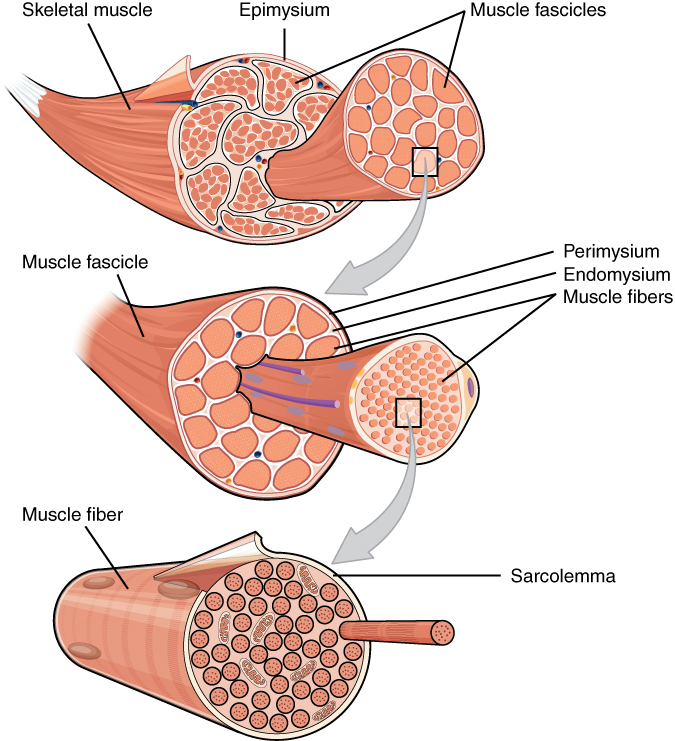
\includegraphics[width=0.5\linewidth]{assets/muscle} 

}

\caption{Structure of a skeletal muscle, muscle fascicle and muscle fiber. Figure from the OpenStax \textit{Anatomy and Physiology} Textbook. Download for free at \url{https://cnx.org/contents/14fb4ad7-39a1-4eee-ab6e-3ef2482e3e22@15.1}.}\label{fig:muscle}
\end{figure}

The muscle fiber is surrounded by a membrane, the \emph{sarcolemma} (see Figure \ref{fig:muscle}). Under resting conditions, the voltage inside the membrane is around -90mV, relative to the outside. This voltage results from a particular combination of sodium (\(\text{Na}^{+}\)), potassium (\(\text{K}^{+}\)), chloride (\(\text{Cl}^{-}\)), and other anions. At rest, the concentration of \(\text{Na}^{+}\) is relatively high outside the membrane and relatively low inside the membrane. The concentration of \(\text{K}^{+}\) follows an opposite pattern, with a greater concentration inside the membrane, and a lower concentration outside the membrane.

\hypertarget{the-motor-action-potential}{%
\subsubsection{The motor action potential}\label{the-motor-action-potential}}

Because muscle membranes can change their electrical state, muscle fibers are excitable tissues. When a muscle fiber is depolarised, the \emph{membrane potential} produces a response called the \emph{muscle fiber ation potential} or more generally the \emph{motor action potential} (MAP). The generated action potential proceeds along the muscle fiber in both directions from the neuromuscular junction (Kamen \& Gabriel, \protect\hyperlink{ref-kamen_essentials_2010}{2010}).\footnote{The \emph{neuromuscular junction} is the site where the motoneuron meets the muscle fiber.} In the first phase of the MAP, the \(\text{Na}^{+}\) permeability increases dramatically, inducing a massive income of \(\text{Na}^{+}\) into the cell. This results in a temporary inversion of the cell polarity (see Figure \ref{fig:mfap}).

\begin{figure}

{\centering 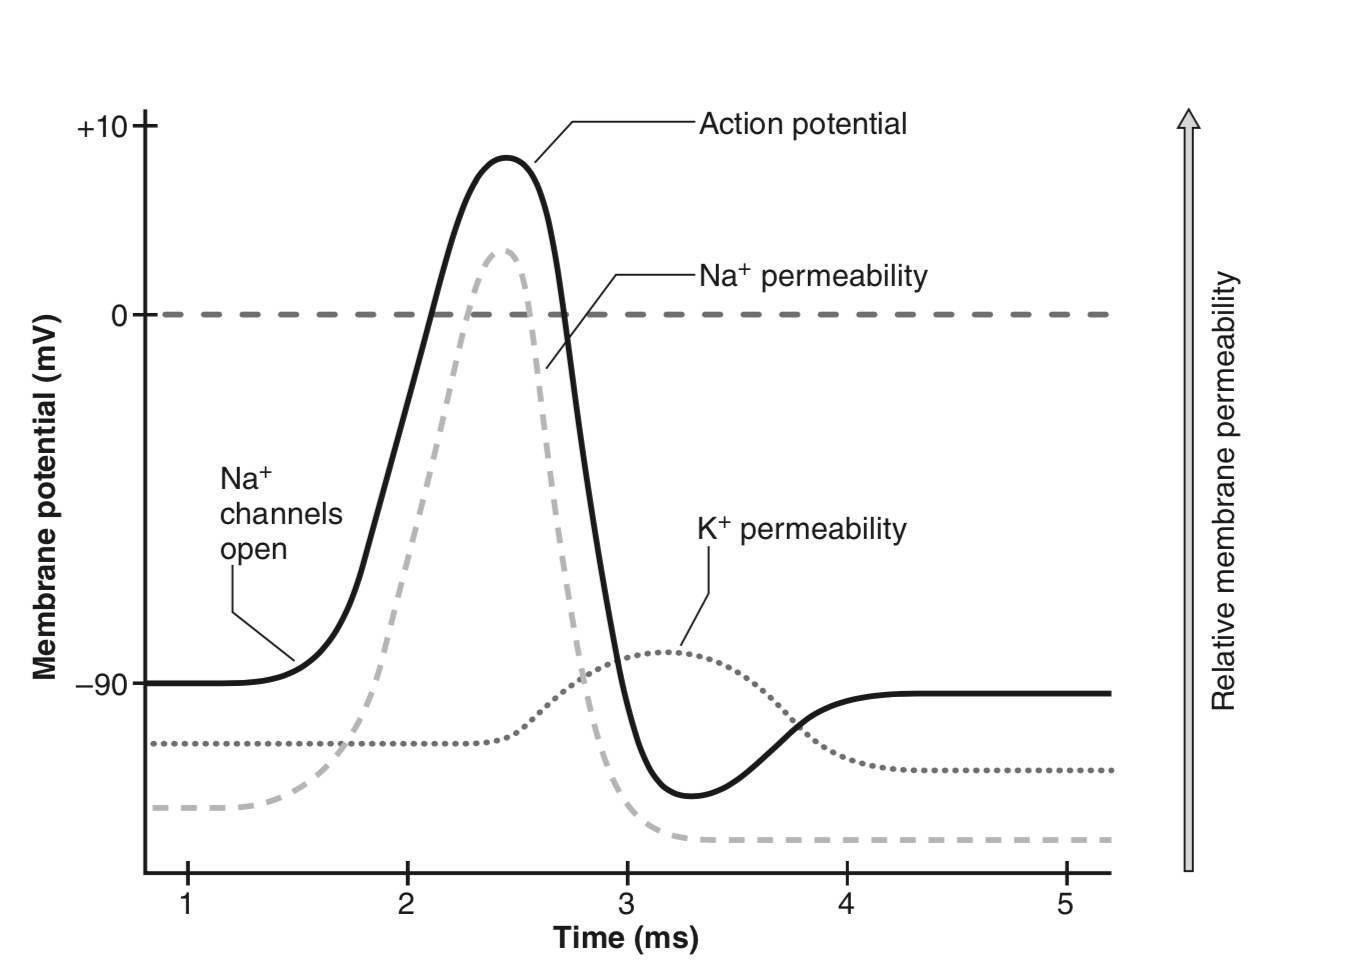
\includegraphics[width=0.75\linewidth]{assets/mfap} 

}

\caption{Time course of a motor action potential (figure from Kamen \& Gabriel, 2010).}\label{fig:mfap}
\end{figure}

The MAP is followed by a \emph{refractory period}, characterised by a decrease in membrane excitability. This refractory period can be further decomposed in an \emph{absolute} refractory period during which all \(\text{Na}^{+}\) channels are closed, and a \emph{relative} refractory period where some \(\text{Na}^{+}\) channels are open (but to a lesser extent than before the MAP). Interestingly, this after-impulse hyperpolarisation limits the frequency of MAPs (Kamen \& Gabriel, \protect\hyperlink{ref-kamen_essentials_2010}{2010}).

\hypertarget{the-motor-unit}{%
\subsubsection{The motor unit}\label{the-motor-unit}}

The \emph{motor unit} is the smallest controllable muscular unit. It consists in a single \(\alpha\)-motoneuron, its neuromuscular junction, and all the muscle fibers it innervates. The number of motor units and their \emph{innervation ratio} (i.e., the number of muscle fibers per motor unit) can vary by muscle. Because a single motoneuron can innervate multiple muscle fibers, the firing of a single motoneuron results in the simultaneous discharge of many muscle fibers. The \emph{motor unit action potential} (MUAP) is the electric field resulting from the sum of the electric fields emitted by each fiber of the motor unit. In other words, it represents the spatiotemporal summation of individual MAPs originating from muscle fibers that are sufficiently close to a given electrode. This generates a \emph{train} of MUAPs, called \emph{motor unit action potential trains} (MUAPTs). The mixture of MUAPTs coming from different motor units constitute the raw EMG signal (cf.~Figure \ref{fig:muap}).

\begin{figure}

{\centering 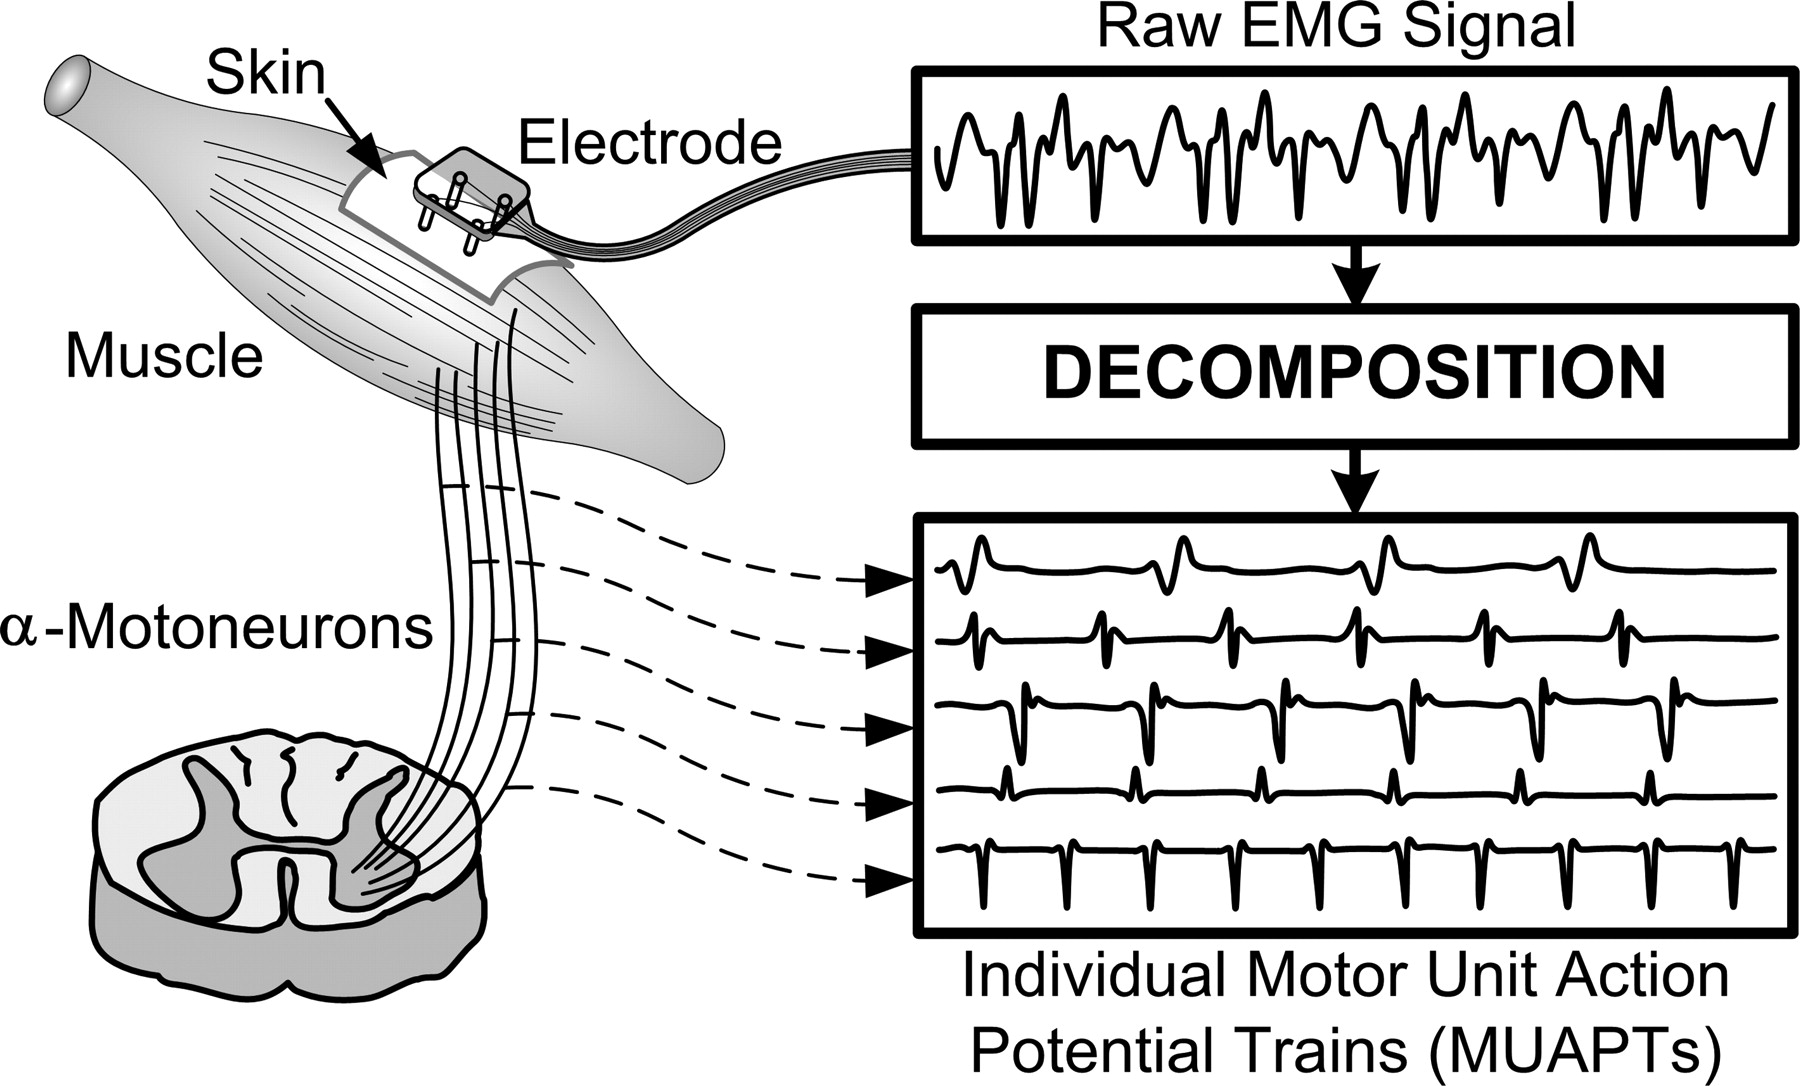
\includegraphics[width=0.75\linewidth]{assets/muap} 

}

\caption{Motor unit action potential representation (figure from De Luca et al., 2006).}\label{fig:muap}
\end{figure}

To sum up, the EMG signal results from a mixture of recruited motor units: it is composed of the sum of several to many MUAPTs. This signal can vary considerably because of factors such as the muscle length (Babault, Pousson, Michaut, \& Van Hoecke, \protect\hyperlink{ref-babault_effect_2003}{2003}), the distance between the muscle fiber (of interest) and the electrode, the fiber length or the muscle temperature. In the next section, we discuss in more details how this signal can be acquired.

\hypertarget{emg-instrumentation-and-recording}{%
\subsection{EMG instrumentation and recording}\label{emg-instrumentation-and-recording}}

Myoelectric measurements have a long history, starting in the XVII and XVIII centuries with the classical observations that muscle contraction can generate electricity and that electrical impulses can generate muscle contraction. The term of electromyography and the first EMG measures were realised at the end of the XIXth century, and the quality of EMG measurements did not cease to improve since (see Raez, Hussain, \& Mohd-Yasin, \protect\hyperlink{ref-raez_techniques_2006}{2006}, for a brief historical perspective).

Two main types of sensors have been used to record EMG signals, varying by their invasiveness. First, \emph{indwelling} (intramuscular) recordings can be acquired via electrodes directly inserted into the muscle. This form of EMG is mostly used in rehabilitation, for diagnosis of muscle function and to examine nerve conduction (Fridlund \& Cacioppo, \protect\hyperlink{ref-fridlund_guidelines_1986}{1986}). Second, \emph{surface electromyography} can be recorded at the surface of the skin. Each method is associated with its own type of sensors, its own advantages and disadvantages. Surface electrodes have the advantage of being easy to use and non-invasive. However, their use is limited to (large and) superficial muscles. Moreover, because of the phenomenon of \emph{cross-talk},\footnote{The phenomenon of \emph{cross-talk} can be defined as the mixing of the electrical activity of the muscle of interest with the electrical activity of adjacent or distant muscles, that are not of primary interest.} it is difficult to isolate the activity of specific muscles using surface EMG. On the opposite, intramuscular EMG (that can be recorded via a single needle or two wires implanted directly into the muscle) are highly selective and can sometimes record the activity of individual motor units. In addition, indwelling recordings are not submitted to \emph{tissue filtering} (i.e., the fact that muscles tissues act as low-pass filters), in contrast to surface recordings.

In reason of the important intercrossing and superposition of facial muscles, surface EMG recorded over facial muscles does not generally represent the activity of a single muscle, but rather a mixture of muscles activations (De Luca, \protect\hyperlink{ref-de_luca_use_1997}{1997}; Rapin, \protect\hyperlink{ref-Rapin2011}{2011}). As a result, it is usually inappropriate, when using surface EMG, to attribute the recorded activity to a single muscle (Fridlund \& Cacioppo, \protect\hyperlink{ref-fridlund_guidelines_1986}{1986}). Whereas for the sake of simplicity, we designate sensors by the name of the underlying muscle of interest (e.g., \enquote{FRO} for the \emph{frontalis} muscle), it should be kept in mind that these sensors reflect the activity of \enquote{sites}, rather than the activity of single muscles.

Aside from \emph{cross-talk}, many other factors can affect the EMG signals. These factors are usually described under three main categories (for more details, see De Luca, \protect\hyperlink{ref-de_luca_use_1997}{1997}):

\begin{itemize}
\item
  The \emph{causative factors}, that have a basic effect on EMG signals. These factors can be further subdivided into two classes: i) the \emph{extrinsic} factors, including factors such as the type of electrode (e.g., size, shape, placement) or the inter-electrode distance and ii) the \emph{intrinsic} factors such as physiological or anatomical factors (e.g., fiber type, fiber diameter, blood flow).
\item
  The \emph{intermediate factors}. These are the physiological phenomena that are influenced by one or more of the causative factors and that in turn influence the deterministic factors, such as the conduction velocity, spatial filtering or the signal \emph{cross-talk}.
\item
  Finally, the \emph{deterministic factors} are influenced by the intermediate factors and have a direct effect on the EMG signal. These include the number of active motor units or the amplitude, duration and shape of the MUAPs.
\end{itemize}

All these factors contribute to modulating both the amplitude of the EMG signal and its spectral properties (e.g., its mean or median frequency). The importance of these perturbating factors should be acknowledged and controlled as far as possible. In our work, we use state-of-the art surface EMG apparatus, specifically developed to tackle these issues, as well as standardised procedures (more details regarding the EMG apparatus are provided in Chapters \ref{chap3} to \ref{chap5}).

\hypertarget{emg-signal-processing}{%
\subsection{EMG signal processing}\label{emg-signal-processing}}

The raw EMG signal is a stochastic train of MUAPs. As put by Fridlund \& Cacioppo (\protect\hyperlink{ref-fridlund_guidelines_1986}{1986}), \enquote{when heard through a speaker, the raw EMG signal sounds like popcorn popping}. Therefore, it is usually unsuitable for immediate quantification. In order to illustrate what the EMG signal looks like, we simulated EMG data based on a standard algorithm implemented in the \texttt{biosignalEMG} package (Guerrero \& Macias-Diaz, \protect\hyperlink{ref-R-biosignalEMG}{2018}). This simulated EMG signal is represented in Figure \ref{fig:emgplot1}.

\begin{figure}

{\centering 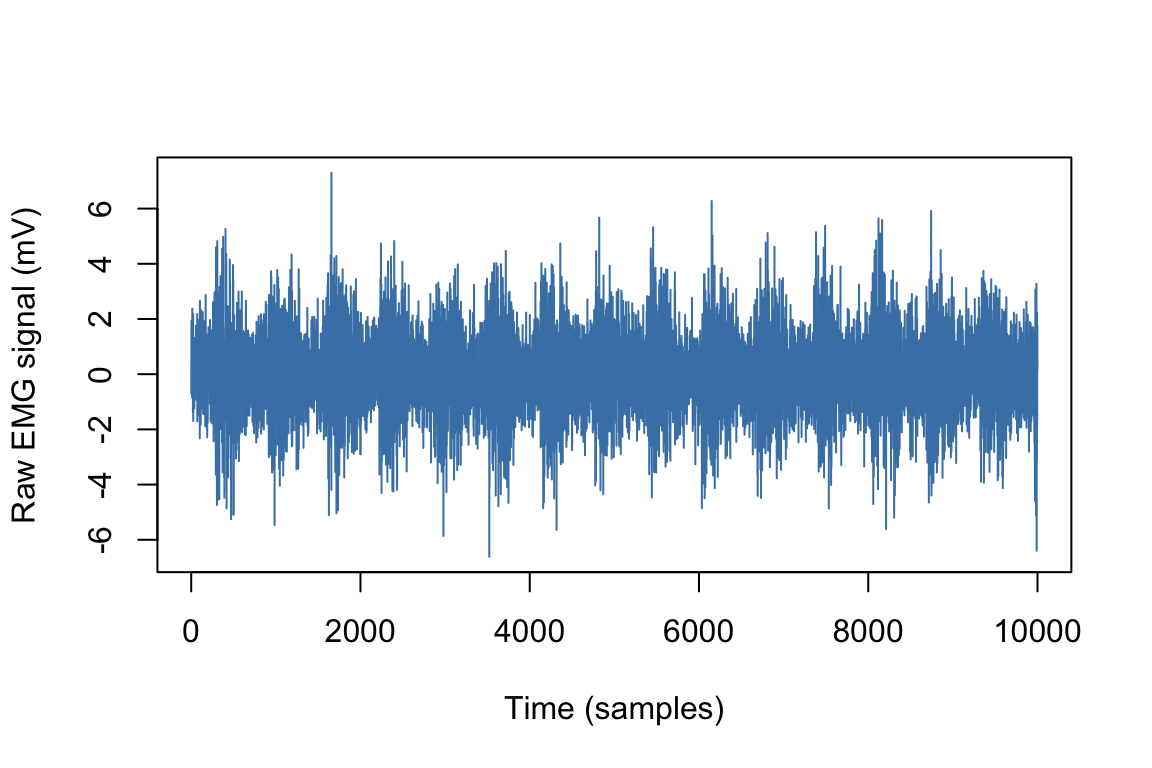
\includegraphics[width=1\linewidth]{02-chap2_files/figure-latex/emgplot1-1} 

}

\caption{Simulated EMG signal.}\label{fig:emgplot1}
\end{figure}

We usually rectify the EMG signal by taking its absolute value and subtracting the mean in order to correct for any offset (bias) present in the raw data. The result of this operation is represented in Figure \ref{fig:emgplot2}.

\begin{figure}

{\centering 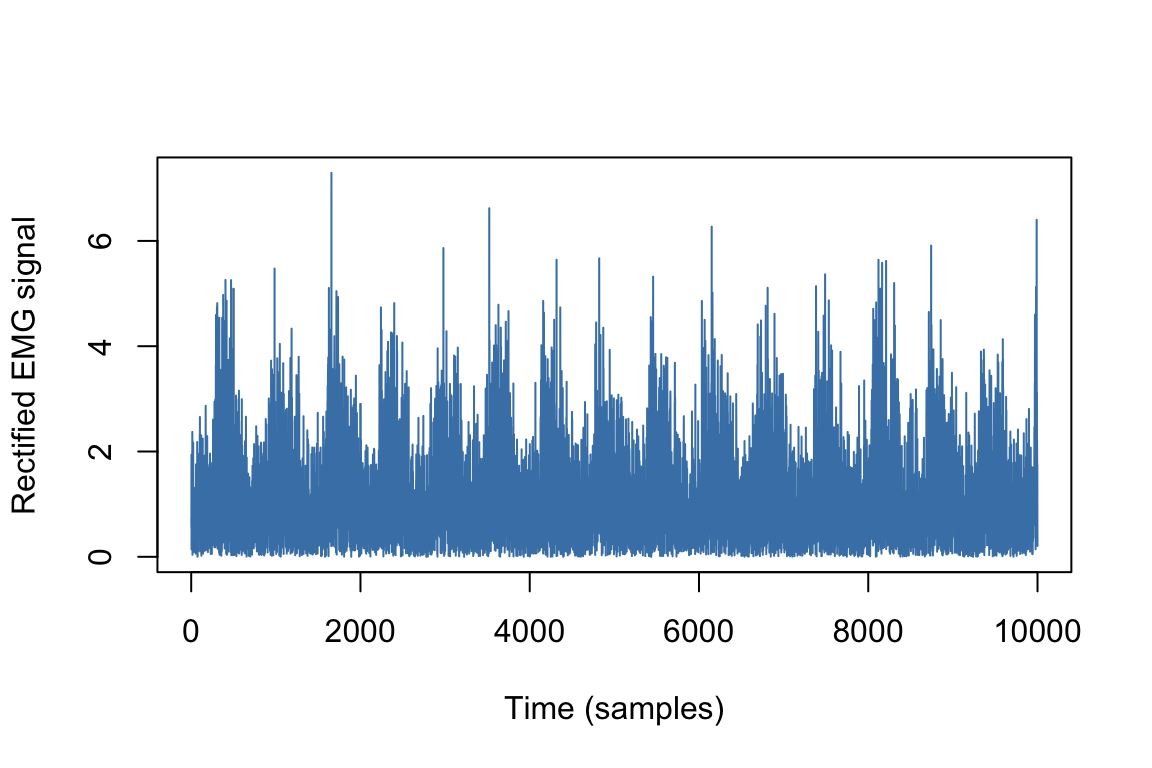
\includegraphics[width=1\linewidth]{02-chap2_files/figure-latex/emgplot2-1} 

}

\caption{Rectified EMG signal.}\label{fig:emgplot2}
\end{figure}

Then, the signal is usually low-pass filtered, with a cut-off frequency depending on the nature of the study. From there, two main measures can be used to represent the magnitude of the muscle activity.\footnote{But see for instance Phinyomark, Nuidod, Phukpattaranont, \& Limsakul (\protect\hyperlink{ref-phinyomark_feature_2012}{2012}), for a brief overview of other features that can be extracted from the surface EMG signal.} The first one is the \emph{mean absolute value} (MAV), which is computed over a specific interval and where \(|x_{n}|\) is the absolute value of a datum of EMG in the data window.

\[MAV = \frac{1}{N} \sum_{n=1}^{N} | x_{n} |\]

The unit of measurement is usually the \(mV\) and the MAV calculation is generally similar to the numerical formula for integration (Kamen \& Gabriel, \protect\hyperlink{ref-kamen_essentials_2010}{2010}). The second one is the \emph{root-mean-square} (RMS) amplitude:

\[RMS = \sqrt{ \frac{1}{N} \sum_{n=1}^{N} x^{2}_{n} }\]

where \(x^{2}_{n}\) is the squared value of each EMG datum and has both physical and physiological meanings. Put broadly, the RMS it taken to reflect the level of the physiological activities in the motor unit during contraction. Both the MAV and the RMS are illustrated in Figure \ref{fig:emgplot3}.

\begin{figure}

{\centering 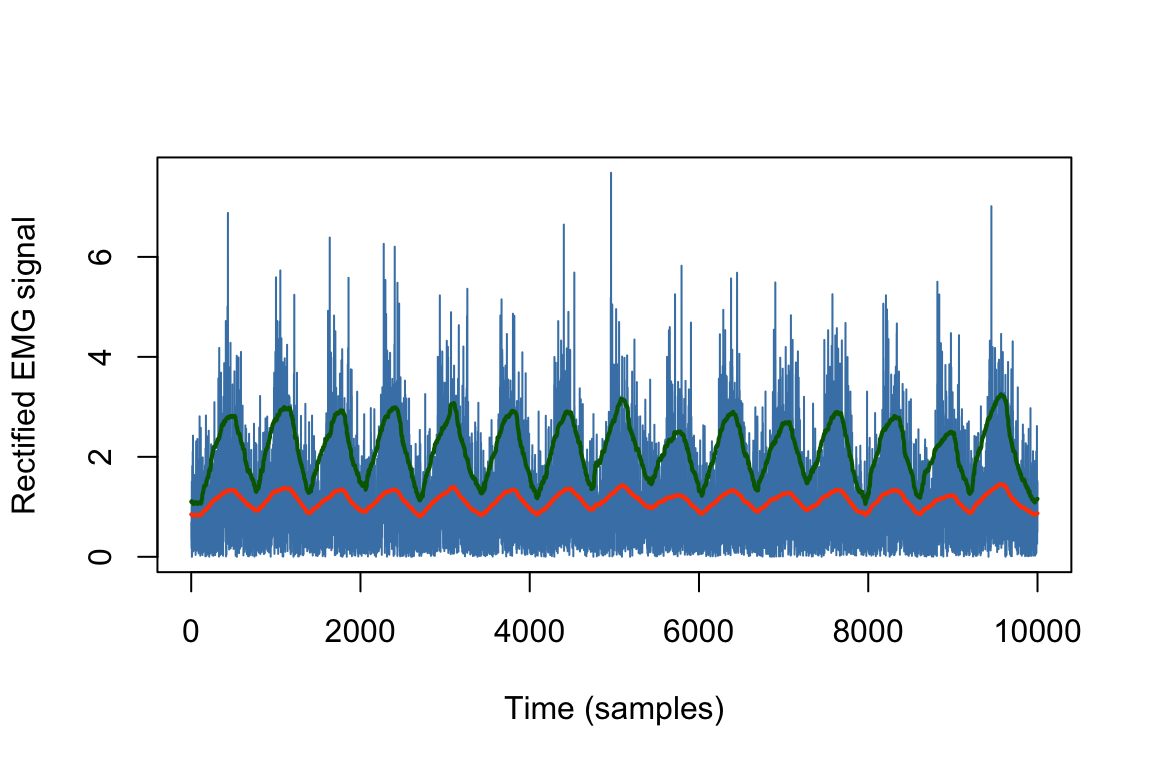
\includegraphics[width=1\linewidth]{02-chap2_files/figure-latex/emgplot3-1} 

}

\caption{Illustration of the MAV (in orange) and RMS (in green) values. These two features are usually highly correlated but differ in magnitude. More precisely, the RMS is proportional to the MAV when the signal has a Gaussian shape.}\label{fig:emgplot3}
\end{figure}

These features provide the \emph{envelope} of the EMG signal and therefore provide insights about the \emph{amplitude} of the EMG signal. This envelope can then be summarised (e.g., via its mean or median) over a period of interest (e.g., during the utterance of some phoneme).

\hypertarget{statistical-modelling-and-statistical-inference}{%
\section{Statistical modelling and statistical inference}\label{statistical-modelling-and-statistical-inference}}

\hypertarget{limitations-of-the-standard-statistical-approach-in-psychology}{%
\subsection{Limitations of the standard statistical approach in Psychology}\label{limitations-of-the-standard-statistical-approach-in-psychology}}

Numerous authors have highlighted the limitations inherent to the Null-Hypothesis Significance Testing (NHST) approach and the (exclusive) reliance on \emph{p}-values and significance testing (e.g., Bakan, \protect\hyperlink{ref-bakan_test_1966}{1966}; Gigerenzer, \protect\hyperlink{ref-Gigerenzer2004}{2004}; Kline, \protect\hyperlink{ref-Kline2004}{2004}; Lambdin, \protect\hyperlink{ref-Lambdin2012}{2012}; Meehl, \protect\hyperlink{ref-meehl_theory-testing_1967}{1967}; Trafimow et al., \protect\hyperlink{ref-trafimow_manipulating_2018}{2018}). Considering these limitations, some authors have recommended to push away significance testing and to develop the use of effect size estimates and confidence intervals in order to favour accumulation of evidence and a meta-analytical mode of thinking (e.g., Cumming, \protect\hyperlink{ref-Cumming2012}{2012}, \protect\hyperlink{ref-cumming_new_2014}{2014}).

However, the apparent superiority of confidence intervals over \emph{p}-values is an illusion. Indeed, as noted by many observers, confidence intervals are simply inverted significance tests. In other words, the confidence interval represents the range of values that are significant at some \(\alpha\) level. Therefore, compared to a \emph{p}-value, a confidence interval does not bring \emph{any} new inferential value. Moreover, its interpretation might be as hard as the interpretation of \emph{p}-values. For instance, contrary to a widely shared belief, confidence intervals do not contain the \((1 - \alpha) \cdot 100\)\% most probable values of the parameter (e.g., Morey, Hoekstra, Rouder, Lee, \& Wagenmakers, \protect\hyperlink{ref-morey_fallacy_2015}{2015}; Nalborczyk et al., \protect\hyperlink{ref-nalborczyk_pragmatism_2019}{2019}\protect\hyperlink{ref-nalborczyk_pragmatism_2019}{b}).

That being said, it is fair to acknowledge that using confidence intervals (instead of or in addition to single \emph{p}-values) do shift the emphasis from a mechanical (mindless) point-hypothesis testing procedure to a more careful consideration of the range of values that are \emph{compatible} with some hypothesis. More importantly, it emphasises the uncertainty that accompanies every statistical procedure. Indeed, we think that most of the caveats that are attributed to a specific statistical procedure (e.g., to NHST) are really caveats of the way it is used. Namely, the fact that it is used in a categorical and absolute way. This tendency has been coined as \emph{dichotomania} (i.e., the tendency to consider that results are either present --if significant-- or absent --if non-significant), or \emph{trichotomania} (e.g., when considering evidence ratios thresholds).

These biases have been highlighted by many statisticians in the past (e.g., Wasserstein \& Lazar, \protect\hyperlink{ref-wasserstein_asas_2016}{2016}). Very recently, \emph{The American Statistician} published a special issue on \emph{Moving to a Wold Beyond \enquote{p\textless.05}}, with the intention to provide new recommendations for users of statistics (e.g., researchers, policy makers, journalists). This issue comprises 43 original papers aiming to provide new guidelines and practical alternatives to the mindless use of statistics. In the accompanying editorial, Wasserstein, Schirm, \& Lazar (\protect\hyperlink{ref-wasserstein_moving_2019}{2019}) summarise these recommendations in the form of the ATOM guidelines: \enquote{\textbf{A}ccept uncertainty. Be \textbf{t}houghtful, \textbf{o}pen, and \textbf{m}odest.} We describe below how our statistical approach might be understood in the light of these core principles.

\begin{itemize}
\item
  \textbf{Accept uncertainty}: we try to represent and to acknowledge uncertainty in our analyses and conclusions. For instance, we do not conclude and/or infer that an effect is either \enquote{present} or \enquote{absent}, but we report the \emph{estimated} magnitude of the effect and the uncertainty that comes with this estimation. Additionally, when relevant, we report probabilistic statements based on the posterior distribution.
\item
  \textbf{Be thoughtful}: for each analysis opportunity (i.e., for each dataset to analyse), we consider what would be the most appropriate modelling strategy but we also acknowledge that there is no unique best way to analyse a given dataset. In most empirical chapters, we clearly distinguish between confirmatory (preregistered) and exploratory (non-preregistered) statistical analyses. We routinely evaluate the \emph{validity} of the statistical model (and of its assumptions) and we are suspicious of statistical \emph{defaults}. We try to consider the \emph{practical} significance of the results, rather than their \emph{statistical} significance. We use a variety of statistics (e.g., effect sizes, interval estimates, information criteria) to obtain a more diverse picture of the meaning of the results.
\item
  \textbf{Be open}: the soundness of a statistical procedure (and more generally, of an inferential procedure) can only be evaluated if it is made transparent to peers and readers for critical examination. Therefore, we take some space in the next section (but also in each experimental chapter) to motivate our statistical modelling decisions. We also make all \texttt{R} scripts available to ensure the reproducibility of the analyses. We try to be exhaustive in the way we report our analyses and we beware of shortcuts than could hinder important information to the reader.
\item
  \textbf{Be modest}: we recognise that there is no unique \enquote{true statistical model} and we discuss the limitations of our analyses and conclusions. We also recognise that scientific inference is much broader than statistical inference (e.g., a degenerative research program is much more informative than a non-significant \emph{p}-value). We try not to conclude anything from a single study without the warranted uncertainty.
\end{itemize}

To sum up, we try to acknowledge the uncertainty that accompanies every (statistical) inference. In the next section, we present in more details what our approach does entail and we introduce some key technical concepts.

\hypertarget{our-statistical-approach}{%
\subsection{Our statistical approach}\label{our-statistical-approach}}

In brief, we tried to move from the point-hypothesis mechanical testing to an approach that emphasises parameter estimation, model comparison, and continuous model expansion (e.g., Cumming, \protect\hyperlink{ref-Cumming2012}{2012}, \protect\hyperlink{ref-cumming_new_2014}{2014}; Gelman et al., \protect\hyperlink{ref-gelman_bayesian_2013}{2013}; Gelman \& Hill, \protect\hyperlink{ref-gelman_data_2006}{2006}; Judd, McClelland, \& Ryan, \protect\hyperlink{ref-judd_data_2009}{2009}; Kruschke, \protect\hyperlink{ref-kruschke_doing_2015}{2015}; Kruschke \& Liddell, \protect\hyperlink{ref-kruschke_bayesian_2018}{2018}\protect\hyperlink{ref-kruschke_bayesian_2018}{a}, \protect\hyperlink{ref-kruschke_bayesian_2018-1}{2018}\protect\hyperlink{ref-kruschke_bayesian_2018-1}{b}; McElreath, \protect\hyperlink{ref-R-rethinking}{2016}\protect\hyperlink{ref-R-rethinking}{a}). In other words, our approach can be defined as a \emph{statistical modelling} approach rather than a \emph{statistical testing} approach. It means that we try to \emph{model} the data (or rather the process that generated the data), rather than to \enquote{test} it. We carefully consider what could be the process that generated the data and we try to model it appropriately. For instance, we do not fit reaction time data, Likert data, or electromyographic data using the same model, as this practice would lead to high rates of erroneous inferences.

Throughout this work, we use Bayesian statistical modelling, not by dogmatism, but because we think the Bayesian approach provides richer inferences than the frequentist one. The main advantage of the Bayesian approach is the explicit use of probability to model the uncertainty (see Box \ref{logic}). By doing so, the Bayesian approach permits to evaluate the probability of a parameter (or a vector of parameters) \(\theta\), given a set of data \(y\):

\[p(\theta|y) = \frac{p(y|\theta)p(\theta)}{p(y)}\]

Using this equation (known as Bayes' theorem), a probability distribution \(p(\theta|y)\) can be derived (called the \emph{posterior distribution}), that reflects knowledge about the parameter, given the data and the prior information. This distribution is the goal of any Bayesian analysis and contains all the information needed for inference.

The term \(p(\theta)\) corresponds to the \emph{prior distribution}, which specifies the prior information about the parameters (i.e., what is known about \(\theta\) before observing the data) as a probability distribution. The left hand of the numerator \(p(y|\theta)\) represents the \emph{likelihood}, also called the \emph{sampling distribution} or \emph{generative model}, and is the function through which the data affect the posterior distribution. The likelihood function indicates how likely the data are to appear, for each possible value of \(\theta\). Finally, \(p(y)\) is called the \emph{marginal likelihood}. It is meant to normalise the posterior distribution, that is, to scale it in the \enquote{probability world}. It gives the \enquote{probability of the data}, summing over all values of \(\theta\) and is described by \(p(y) = \sum_{\theta} p(\theta) p(y|\theta)\) for discrete parameters, and by \(p(y) = \int p(\theta) p(y|\theta) d\theta\) in the case of continuous parameters.

All this pieced together shows that the result of a Bayesian analysis, namely the posterior distribution \(p(\theta|y)\), is given by the product of the information contained in the data (i.e., the likelihood) and the information available before observing the data (i.e., the prior). This constitutes the crucial principle of Bayesian inference, which can be seen as an updating mechanism. To sum up, Bayes' theorem allows a prior state of knowledge to be updated to a posterior state of knowledge, which represents a compromise between the prior knowledge and the empirical evidence.

\vspace{2mm}

\begin{mybox}[label = logic]{Probability theory as extended logic}

Probability theory has been argued to be nothing more than \textit{extended logic}. In other words, it generalises the rules of logic that apply to discrete events (e.g., TRUE or FALSE events) to continuous events. By doing this move, probability theory gives a way to represent and to quantify the \textit{uncertainty}. Importantly, the rules of probability have the same status as the rules of logic: these rules can be used to derive statements (conclusions) that are guaranteed to be correct given that some premises are correct.\\

Bayesian statistics can simply be presented as an application of probability theory to statistical analysis. Whereas the dependence of the inferential conclusions on prior assumptions is sometimes presented as a downside of this type of analysis, it is precisely what makes them \textit{optimal} or \textit{coherent} (in the sense of respecting the rules of probability). As put by Vandekerckhove (2018), the claim that Bayesian methods would be invalidated by their reliance on prior assumptions would be akin to conclude that logical deductions are somehow invalidated because they depend on premises.

\end{mybox}

We also use \emph{multilevel models} (also known as \emph{mixed-models}) to handle complex dependency structures and to obtain more precise estimates. A more accurate description of Bayesian multilevel models is outside the scope of this introductory section but the interested reader is redirected toward several existing tutorial papers (e.g., Nalborczyk et al., \protect\hyperlink{ref-nalborczyk_introduction_2019}{2019}\protect\hyperlink{ref-nalborczyk_introduction_2019}{a}; Nicenboim \& Vasishth, \protect\hyperlink{ref-nicenboim_statistical_2016}{2016}; Sorensen, Hohenstein, \& Vasishth, \protect\hyperlink{ref-sorensen_bayesian_2016}{2016}) and Appendix \ref{appendix-brms}. Throughout this work, we also make use of several tools with very distinct properties and uses. For instance, we use Bayes factors (BFs) to quantify the relative evidence for a statistical hypothesis (see Box \ref{BF}), we use information criteria to assess the predictive abilities of our models (see Box \ref{IC}), we use posterior predictive checks as well as a diagnostics tools (e.g., convergence indexes, trace plots) to assess the validity of our models, and we use summary statistics when appropriate to convey the meaning of the main results.

\vspace{2mm}

\begin{mybox}[label = BF]{What is a Bayes factor ?}

It is a rule in statistics that every statistics has already been suggested as the \textit{new statistics}. Confidence intervals have been suggested as a replacement to \textit{p}-values, being purportedly more informative and less difficult to interpret. Credible intervals have been suggested as a replacement to confidence intervals, for roughly the same reasons. Bayesian hypothesis testing through Bayes factors (BFs) has also been suggested as a replacement for frequentist hypothesis testing. It has been argued that they permit a richer inference and that they come with a more straightforward interpretation. Whereas this might be true, they nonetheless come with their lot of misinterpretations.\\

To highlight what BFs are and what they are not, it might be useful to write down the formula used to compute them. To this end, it is useful to write the Bayes rule in its \textit{odds form}, making the BF explicitly visible:

$$\underbrace{\dfrac{p(H_{0}|D)}{p(H_{1}|D)}}_{posterior\ odds} = \underbrace{\dfrac{p(D|H_{0})}{p(D|H_{1})}}_{Bayes\ factor} \times \underbrace{\dfrac{p(H_{0})}{p(H_{1})}}_{prior\ odds}$$

This equation reveals that the \textit{posterior odds}, the ratio of the posterior probability (i.e., how much more probable is hypothesis 1 ($H_{1}$) as compared to hypothesis 2 ($H_{2}$), after seeing the data $D$), is equal to the ratio of the probability of the data given the first hypothesis and the probability of the data given the second hypothesis, multiplied by the \textit{prior odds} (i.e., how much more probable was hypothesis 1 ($H_{1}$) as compared to hypothesis 2 ($H_{2}$), before seeing the data $D$).\\ 

Importantly, what we consider as \textit{evidence} in the Bayesian framework is also known as a \textit{marginal likelihood} and represents the information contained in the data, weighted by the prior information. It is a sum when parameters are discrete or an integral when parameters are continuous.

$$\text{evidence}\ = p(D|H) = \int p(\theta|H) p(D|\theta,H) \text{d}\theta$$

Therefore, the BF does not indicate how much "probable" a hypothesis is, or how much more probable a hypothesis is, compared to another one (this would be to conflate the BF with the posterior odds). Instead, the BF can be (should be) interpreted either i) as a ratio of two \textit{marginal likelihoods} (i.e., a ratio of \textit{evidence}) or ii) as an updating factor, indicating how we should reallocate credibility from prior knowledge (what we knew before seeing the data) to posterior knowledge (what we know after seeing the data).

\end{mybox}

Bayes factors are often said to have desirable \emph{asymptotic} (i.e., when the number of observations is very large) properties. Indeed, they are \emph{consistent} for model identification. It means that if a \enquote{true} statistical model is in the set of models that are compared, using a BF will usually lead to selecting this \enquote{true} model with a probability approaching 1 with increasing sample size. Whereas this seems as an appealing property or not depends on the underlying statistical philosophy. Indeed, one could question whether it is sensible to assume a \enquote{true model} (an oxymoron) in real life, especially in the social sciences (e.g., Burnham \& Anderson, \protect\hyperlink{ref-burnham_model_2002}{2002}, \protect\hyperlink{ref-burnham_multimodel_2004}{2004}). As Findley (\protect\hyperlink{ref-findley_unbiasedness_1985}{1985}) notes: \emph{\enquote{{[}\ldots{]} consistency can be an undesirable property in the context of selecting a model}}. A more realistic question is then not to look for the \enquote{true} model, but rather for the \emph{best} model for some practical purpose.

The usefulness of information criteria comes from them being approximations of the \emph{out-of-sample deviance} (see Box \ref{IC}). In the present PhD work, we used generalisations of the AIC (especially the WAIC and LOOIC) that also approximate the \emph{out-of-sample deviance} and as such give an indication of how good/bad a model is to predict future (i.e., non-observed) data.

\vspace{2mm}

\begin{mybox}[label = IC]{Information criteria}

Hirotugu Akaike noticed that the negative log-likelihood of a model + 2 times its number of parameters was approximately equal to the \textbf{out-of-sample deviance} of a model, which lead to what is nowadays famously known as the \textit{Akaike information criterion} (AIC):

$$\text{AIC} = \underbrace{\underbrace{-2\log(\mathcal{L}(\hat{\theta}|\text{data}))}_{\text{in-sample deviance}} + 2K}_{\approx\ \text{out-of-sample deviance}}$$

where $K$ is the number of parameters of the model and the \textit{deviance} is a measure of discrepancy between the data and the model. Interestingly, we can make a distinction between two types of deviances.\\

First, the \textbf{in-sample deviance} indicates how bad a model is to explain the current dataset (the dataset used to fit the model). Second, and more importantly, the \textbf{out-of-sample deviance} indicates how bad a model is to explain a \textbf{future} dataset issued from the same data generation process (the same population).

\end{mybox}

In brief, in the present work, we used various methods but coherently with a few (nuanced) guiding principles. Namely, we favoured a \emph{model comparison} approach (e.g., Burnham \& Anderson, \protect\hyperlink{ref-burnham_model_2002}{2002}, \protect\hyperlink{ref-burnham_multimodel_2004}{2004}; Judd et al., \protect\hyperlink{ref-judd_data_2009}{2009}), we used several statistics when they provide complementary information (e.g., using both posterior probabilities, information criteria or BFs), we assessed the validity of our models (e.g., via posterior predictive checks), we reported these analyses transparently, and we tried to convey uncertainty in our conclusions.

\hypertarget{overview-of-the-following-chapters}{%
\section{Overview of the following chapters}\label{overview-of-the-following-chapters}}

The experiments carried out during this PhD will be presented as five empirical chapters that can be grouped under two main axes. In the first couple of experiments, we used surface electromyography and muscle-specific relaxation to investigate the involvement of the speech motor system during induced verbal and non-verbal rumination (Chapter \ref{chap3} \& \ref{chap4}). In Chapter \ref{chap5}, we used surface electromyography and machine learning algorithms to decode the muscle-specific EMG correlates of inner speech production. In the last couple of experiments, we switched strategy from the \enquote{correlates strategy} to the \enquote{interference strategy}, where the goal was to directly interfere with the activity of the speech motor system. More precisely, we used articulatory suppression to disrupt induced rumination in Chapter \ref{chap6}, and we used articulatory suppression to disrupt either induced rumination or problem-solving in Chapter \ref{chap7}. Finally, in Chapter \ref{chap8}, we summarise the main findings, discuss their implications and suggest ways forward from both a theoretical and an experimental perspective.

\hypertarget{part-experimental-part}{%
\part{Experimental part}\label{part-experimental-part}}

\hypertarget{chap3}{%
\chapter{Orofacial electromyographic correlates of induced verbal rumination}\label{chap3}}

\initial{R}umination is predominantly experienced in the form of repetitive verbal thoughts. Verbal rumination is a particular case of inner speech. According to the \emph{Motor Simulation view}, inner speech is a kind of motor action, recruiting the speech motor system. In this framework, we predicted an increase in speech muscle activity during rumination as compared to rest. We also predicted increased forehead activity, associated with anxiety during rumination. We measured electromyographic activity over the \emph{orbicularis oris superior and inferior}, \emph{frontalis} and \emph{flexor carpi radialis} muscles. Results showed increased lip and forehead activity after rumination induction compared to an initial relaxed state, together with increased self-reported levels of rumination. Moreover, our data suggest that orofacial relaxation is more effective in reducing rumination than non-orofacial relaxation. Altogether, these results support the hypothesis that verbal rumination involves the speech motor system, and provide a promising psychophysiological index to assess the presence of verbal rumination.\footnote{This experimental chapter is a published paper reformatted for the need of this thesis. Source: Nalborczyk, L., Perrone-Bertolotti, M., Baeyens, C., Grandchamp, R., Polosan, M., Spinelli, E., \ldots{} L\oe venbruck, H. (2017). Orofacial Electromyographic Correlates of Induced Verbal Rumination. \emph{Biological Psychology, 127}, 53-63. \url{https://dx.doi.org/10.1016/j.biopsycho.2017.04.013}.}

\hypertarget{introduction}{%
\section{Introduction}\label{introduction}}

As humans, we spend a considerable amount of time reflecting upon ourselves, thinking about our own feelings, thoughts and behaviors. Self-reflection enables us to create and clarify the meaning of past and present experiences (Boyd \& Fales, \protect\hyperlink{ref-boyd_reflective_1983}{1983}; Nolen-Hoeksema et al., \protect\hyperlink{ref-Nolen-Hoeksema2008}{2008}). However, this process can lead to unconstructive consequences when self-referent thoughts become repetitive, abstract, evaluative, and self-critical (Watkins, \protect\hyperlink{ref-Watkins2008}{2008}).

Indeed, rumination is most often defined as a repetitive and recursive mode of responding to negative affect (Rippere, \protect\hyperlink{ref-Rippere1977}{1977}) or life situations (Robinson \& Alloy, \protect\hyperlink{ref-Robinson2003}{2003}). Although rumination is a common process that can be observed in the general population (Watkins, \protect\hyperlink{ref-Watkins2008}{2008}), it has been most extensively studied in depression and anxiety. Depressive rumination has been thoroughly studied by Susan Nolen-Hoeksema, who developed the Response Style Theory (RST, Nolen-Hoeksema, \protect\hyperlink{ref-nolen-hoeksema_responses_1991}{1991}). According to the RST, depressive rumination is characterized by an evaluative style of processing that involves recurrent thinking about the causes, meanings, and implications of depressive symptoms. Even though rumination can involve several modalities (i.e., visual, sensory), it is a predominantly verbal process (Goldwin \& Behar, \protect\hyperlink{ref-goldwin_concreteness_2012}{2012}; McLaughlin et al., \protect\hyperlink{ref-mclaughlin_effects_2007}{2007}). In this study, we focus on verbal rumination, which can be conceived of as a particularly significant form of inner speech.

Inner speech or covert speech can be defined as silent verbal production in one's mind or the activity of silently talking to oneself (Zivin, \protect\hyperlink{ref-zivin_development_1979}{1979}). The nature of inner speech is still a matter of theoretical debate (for a review, see Perrone-Bertolotti et al., \protect\hyperlink{ref-Perrone-Bertolotti2014}{2014}). Two opposing views have been proposed in the literature: the \emph{Abstraction view} and the \emph{Motor Simulation view}. The \emph{Abstraction view} describes inner speech as unconcerned with articulatory or auditory simulations and as operating on an amodal level. It has been described as \enquote{condensed, abbreviated, disconnected, fragmented, and incomprehensible to others} (Vygotsky, \protect\hyperlink{ref-vygotsky_collected_1987}{1987}). It has been argued that important words or grammatical affixes may be dropped in inner speech (Vygotsky, \protect\hyperlink{ref-vygotsky_collected_1987}{1987}) or even that the phonological form or representation of inner words may be incomplete (Dell \& Repka, \protect\hyperlink{ref-dell_errors_1992}{1992}; Sokolov, \protect\hyperlink{ref-sokolov_inner_1972}{1972}). MacKay (\protect\hyperlink{ref-mackay_constraints_1992}{1992}) stated that inner speech is nonarticulatory and nonauditory and that \enquote{Even the lowest level units for inner speech are highly abstract} (p.122).

In contrast with this \emph{Abstraction view}, the physicalist or embodied view considers inner speech production as mental simulation of overt speech production. As such, it can be viewed as similar to overt speech production, except that the motor execution process is blocked and no sound is produced (Grèzes \& Decety, \protect\hyperlink{ref-grezes_functional_2001}{2001}; Postma \& Noordanus, \protect\hyperlink{ref-postma_production_1996}{1996}). Under this \emph{Motor Simulation view}, a continuum exists between overt and covert speech, in line with the continuum drawn by Decety \& Jeannerod (\protect\hyperlink{ref-decety_mentally_1996}{1996}) between imagined and actual actions. This hypothesis has led certain authors to claim that inner speech by essence should share features with speech motor actions (Feinberg, \protect\hyperlink{ref-feinberg_efference_1978}{1978}; Simon R Jones \& Fernyhough, \protect\hyperlink{ref-Jones2007}{2007}). The \emph{Motor Simulation view} is supported by several findings. First, covert and overt speech have comparable physiological correlates: for instance, measurements of speaking rate(Landauer, 1962) and respiratory rate (Conrad \& Schönle, \protect\hyperlink{ref-conrad_speech_1979}{1979}) are similar in both. A prediction of the \emph{Motor Simulation view} is that the speech motor system should be recruited during inner speech. Subtle muscle activity has been detected in the speech musculature using electromyography (EMG) during verbal mental imagery, silent reading, silent recitation (Jacobson, \protect\hyperlink{ref-jacobson_electrical_1931}{1931}; Livesay et al., \protect\hyperlink{ref-livesay_covert_1996}{1996}; McGuigan \& Dollins, \protect\hyperlink{ref-mcguigan_patterns_1989}{1989}; Sokolov, \protect\hyperlink{ref-sokolov_inner_1972}{1972}), and during auditory verbal hallucination in patients with schizophrenia (Rapin et al., \protect\hyperlink{ref-Rapin2013}{2013}\protect\hyperlink{ref-Rapin2013}{b}). Second, it has been shown that covert speech production involves a similar cerebral network as that of overt speech production. Covert and overt speech both recruit essential language areas in the left hemisphere (for a review, see Perrone-Bertolotti et al., \protect\hyperlink{ref-Perrone-Bertolotti2014}{2014}). However, there are differences. Consistent with the \emph{Motor Simulation view} and the notion of a continuum between covert and overt speech, overt speech is associated with more activity in motor and premotor areas than inner speech (e.g., Palmer et al., \protect\hyperlink{ref-palmer_event-related_2001}{2001}). This can be related to the absence of articulatory movements during inner verbal production. In a reciprocal way, inner speech involves cerebral areas that are not activated during overt speech (Basho et al., \protect\hyperlink{ref-basho_effects_2007}{2007}). Some of these activations (cingulate gyrus and superior rostral frontal cortex) can be attributed to the inhibition of overt responses.

These findings suggest that the processes involved in overt speech include those required for inner speech (except for inhibition). Several studies in patients with aphasia support this view: overt speech loss can either be associated with an impairment in inner speech (e.g., Levine, Calvanio, \& Popovics, \protect\hyperlink{ref-levine_language_1982}{1982}; Martin \& Caramazza, \protect\hyperlink{ref-martin_short-term_1982}{1982}) or with intact inner speech: only the later phases of speech production (execution) being affected by the lesion (Baddeley \& Wilson, \protect\hyperlink{ref-baddeley_phonological_1985}{1985}; Marshall, Rappaport, \& Garcia-Bunuel, \protect\hyperlink{ref-marshall_self-monitoring_1985}{1985}; Vallar \& Cappa, \protect\hyperlink{ref-vallar_articulation_1987}{1987}). Geva, Bennett, Warburton, \& Patterson (\protect\hyperlink{ref-geva_discrepancy_2011}{2011}) have reported a dissociation that goes against this view, however. In three patients with chronic post-stroke aphasia (out of 27 patients), poorer homophone and rhyme judgement performance was in fact observed in covert mode compared with overt mode. A limitation of this study, though, was that the task was to detect rhymes in written words, which could have been too difficult for the patients. To overcome this limitation, Langland-Hassan, Faries, Richardson, \& Dietz (\protect\hyperlink{ref-langland-hassan_inner_2015}{2015}) have tested aphasia patients with a similar task, using images rather than written words. They also found that most patients performed better in the overt than in the covert mode. They inferred from these results that inner speech might be more demanding in terms of cognitive and linguistic load, and that inner speech may be a distinct ability, with its own neural substrates. We suggest an alternative interpretation to this dissociation. According to our view, rhyme and homophone judgements rely on auditory representations of the stimuli (e.g., Paulesu, Frith, \& Frackowiak, \protect\hyperlink{ref-paulesu_neural_1993}{1993}). Overt speech provides a strong acoustic output that is fed back to the auditory cortex and can create an auditory trace, which can be used to monitor speech. In the covert mode, the auditory output is only mentally simulated, and its saliency in the auditory system is lesser than in the overt mode. This is in accordance with the finding that inner speech is associated with reduced sensory cortex activation compared with overt speech (Shuster \& Lemieux, \protect\hyperlink{ref-shuster_fmri_2005}{2005}). In patients with aphasia, the weakened saliency of covert auditory signals may be accentuated for two reasons: first, because of impairment in the motor-to-auditory transformation that produces the auditory simulation, and second, because of associated auditory deficits. Therefore, according to our view, the reduced performance observed in rhyme and homophone judgement tasks in the covert compared with the overt mode in brain-injured patients, simply indicates a lower saliency of the auditory sensations evoked during inner speech compared with the actual auditory sensations fed back during overt speech production. In summary, these findings suggest that overt and covert speech share common subjective, physiological and neural correlates, supporting the claim that inner speech is a motor simulation of overt speech.

However, the \emph{Motor Simulation view} has been challenged by several experimental results. Examining the properties of errors during the production of tongue twisters, Oppenheim \& Dell (\protect\hyperlink{ref-oppenheim_motor_2010}{2010}) showed that speech errors display a lexical bias in both overt and inner speech. According to these researchers, errors also display a phonemic similarity effect (or articulatory bias), a tendency to exchange phonemes with common articulatory features, but this second effect is only observed with overt speech or with inner speech accompanied with mouthing. This has led Oppenheim \& Dell (\protect\hyperlink{ref-oppenheim_motor_2010}{2010}) to claim that inner speech is fully specified at the lexical level, but that it is impoverished at lower featural (articulatory) levels. This claim, related to the \emph{Abstraction view}, is still debated however, as a phonemic similarity effect has been found by Corley et al. (\protect\hyperlink{ref-corley_error_2011}{2011}). Their findings suggest that inner speech is in fact specified at the articulatory level, even when there is no intention to articulate words overtly. Other findings however, may still challenge the Motor Simulation view. Netsell, Ashley, \& Bakker (\protect\hyperlink{ref-netsell_inner_2010}{2010}) have examined covert and overt speech in persons who stutter (PWS) and typical speakers. They have found that PWS were faster in covert than in overt speech while typical speakers presented similar overt and covert speech rates. This can be interpreted in favour of the \emph{Abstraction view}, in which inner representations are not fully specified at the articulatory level, which would explain why they are not disrupted in PWS speech. Altogether, these results suggest that full articulatory specification may not always be necessary for inner speech to be produced.

The aim of this study is to examine the physiological correlates of verbal rumination in an attempt to provide new data in the debate between motor simulation and abstraction. A prediction of the \emph{Motor Simulation view} is that verbal rumination, as a kind of inner speech, should be accompanied with activity in speech-related facial muscles, as well as in negative emotion or anxiety-related facial muscles, but should not involve non-facial muscles (such as arm muscles). Alternatively, the \emph{Abstraction view} predicts that verbal rumination should be associated with an increase in emotion-related facial activity, without activity in speech-related muscles and non-facial muscles.

There is strong interest in the examination of physiological correlates of rumination as traditional assessment of rumination essentially consists of self-reported measures. The measurement of rumination as conceptualized by Nolen-Hoeksema (\protect\hyperlink{ref-nolen-hoeksema_responses_1991}{1991}) was operationalized by the development of the Ruminative Response Scale (RRS), which is a subscale of the response style questionnaire (Nolen-Hoeksema \& Morrow, \protect\hyperlink{ref-nolen-hoeksema_prospective_1991}{1991}). The RRS consists of 22 items that describe responses to dysphoric mood that are self-focused, symptom-focused, and focused on the causes and consequences of one's mood. Based on this scale, Treynor et al. (\protect\hyperlink{ref-treynor_rumination_2003}{2003}) have offered a detailed description of rumination styles and more recently, Watkins (\protect\hyperlink{ref-Watkins2008}{2008}) has further characterized different modes of rumination. The validity of these descriptions is nevertheless based on the hypothesis that individuals have direct and reliable access to their internal states. However, self-reports increase reconstruction biases (e.g., Brewer, \protect\hyperlink{ref-rubin_what_1986}{1986}; Conway, \protect\hyperlink{ref-conway_autobiographical_1990}{1990}) and it is well known that participants have a very low level of awareness of the cognitive processes that underlie and modulate complex behaviors (Nisbett \& Wilson, \protect\hyperlink{ref-nisbett_telling_1977}{1977}).

In order to overcome these difficulties, some authors have attempted to quantify state rumination and trait rumination more objectively, by recording physiological or neuroanatomical correlates of rumination (for a review, see Siegle \& Thayer, \protect\hyperlink{ref-papageorgiou_physiological_2003}{2003}). Peripheral physiological manifestations (e.g., pupil dilation, blood pressure, cardiac rhythm, cardiac variability) have been examined during induced or chronic rumination. Vickers \& Vogeltanz-Holm (\protect\hyperlink{ref-vickers_effects_2003}{2003}) have observed an increase in systolic blood pressure after rumination induction, suggesting the involvement of the autonomic nervous system in rumination. Moreover, galvanic skin response has shown to be increased after a rumination induction, in highly anxious women (Sigmon et al., \protect\hyperlink{ref-sigmon_impact_2000}{2000}). According to Siegle \& Thayer (\protect\hyperlink{ref-papageorgiou_physiological_2003}{2003}), disrupted autonomic activity could provide a reliable physiological correlate of rumination. In this line, Key et al. (\protect\hyperlink{ref-Key2008}{2008}) have observed a diminution of the high-frequency component of heart rate variability (HF-HRV) after rumination induction in people with a low tendency to ruminate (see also Woody et al., \protect\hyperlink{ref-woody_brooding_2014}{2014}). A consistent link between perseverative cognition and decreased HRV was also found in a meta-analysis conducted by Ottaviani et al. (\protect\hyperlink{ref-Ottaviani2015}{2015}). Based on these positive results and on suggestions that labial EMG activity may accompany inner speech and therefore rumination, our aim was to examine facial EMG as a potential correlate of rumination and HRV as an index to examine concurrent validity.

In addition to labial muscular activity, we also recorded forehead muscular activity (i.e., \emph{frontalis} muscle) because of its implication in prototypical expression of sadness (e.g., Ekman \& Friesen, \protect\hyperlink{ref-ekman_facial_1978}{1978}; Kohler et al., \protect\hyperlink{ref-kohler_differences_2004}{2004}), reactions to unpleasant stimuli (Jäncke et al., \protect\hyperlink{ref-Jancke1996}{1996}), and anxiety or negative emotional state (Conrad \& Roth, \protect\hyperlink{ref-conrad_muscle_2007}{2007}).\footnote{The \emph{corrugator supercilii} was another potential site, as it is sensitive to negative emotions. However, it has been claimed to be mostly activated for strong emotions such as fear/terror, anger/rage and sadness/grief (Ekman \& Friesen, \protect\hyperlink{ref-ekman_facial_1978}{1978}; Sumitsuji, Matsumoto, Tanaka, Kashiwagi, \& Kaneko, \protect\hyperlink{ref-sumitsuji_electromyographic_1967}{1967}). The rumination induction used in this study was designed to have participants self-reflect and brood over their failure at the I.Q. test. It was not meant to induce such strong emotions. Several studies have reported increased activity in the \emph{frontalis} muscle at rest in anxious or generalized anxiety disorder patients (for a review, see Conrad \& Roth, \protect\hyperlink{ref-conrad_muscle_2007}{2007}). We expected the type of emotional state induced by rumination to be closer to anxiety or worry than to strong emotions like fear, anger or grief. It was therefore more appropriate to record non-speech facial activity in the \emph{frontalis} rather than in the \emph{corrugator.}} Our hypothesis was that \emph{frontalis} activity could be an accurate electromyographic correlate of induced rumination, as a negatively valenced mental process.

In this study, we were also interested in the effects of relaxation on induced rumination. Using a relaxation procedure targeted on muscles involved in speech production is a further way to test the reciprocity of the link between inner speech (verbal rumination) and orofacial muscle activity. If verbal rumination is a kind of action, then its production should be modulated in return by the effects of relaxation on speech effectors. This idea is supported by the results of (among others) Cefidekhanie, Savariaux, Sato, \& Schwartz (\protect\hyperlink{ref-cefidekhanie_interaction_2014}{2014}), who have observed substantial perturbations of inner speech production while participants had to realize forced movements of the articulators.

In summary, the current study aimed at evaluating the \emph{Motor Simulation view} and the \emph{Abstraction view} by using objective and subjective measures of verbal rumination. To test the involvement of the orofacial motor system in verbal rumination, we used two basic approaches. In the first approach, we induced verbal rumination and examined concurrent changes in facial muscle activity (Experiment 1). In the second approach, we examined whether orofacial relaxation would reduce verbal rumination levels (Experiment 2). More specifically, in Experiment 1, we aimed to provide an objective assessment of verbal rumination using quantitative physiological measures. Thus, we used EMG recordings of muscle activity during rumination, focusing on the comparison of speech-related (i.e., two lip muscles − \emph{orbicularis oris superior} and \emph{orbicularis oris inferior}) and speech-unrelated (i.e., forehead −\emph{frontalis}- and forearm − \emph{flexor carpi radialis}) muscles. Under the \emph{Motor Simulation view}, an increase in lip and forehead EMG activity should be observed after rumination induction, with no change in forearm EMG activity, associated with an increase in self-reported rumination. Alternatively, under the \emph{Abstraction view}, an increase in forehead activity should be observed, associated with an increase in self-reported rumination, and no changes in either lip or forearm activity should be noted.

In Experiment 2, in order to assess the reciprocity of the rumination and orofacial motor activity relationship, we evaluated the effects of orofacial relaxation on rumination. More specifically, we compared three kinds of relaxation: i) Orofacial Relaxation (i.e., lip muscles), ii) Arm Relaxation (i.e., to differentiate effects specific to speech-related muscle relaxation) and iii) Story Relaxation (i.e., to differentiate effects specific to attentional distraction). If the \emph{Motor simulation view} is correct, we predicted a larger decrease of lip and forehead muscle activity after an Orofacial Relaxation than after an Arm Relaxation (associated with a larger decrease in self-reported rumination), which should also be larger than after listening to a story. We also predicted that forearm activity should remain stable across the three conditions (i.e., should not decrease after relaxation). Alternatively, if the \emph{Abstraction view} is correct, we predicted that none of the relaxation conditions should have an effect on lip or arm activity, because none of these should have increased after induction. However, we expected to observe a decrease in forehead activity and self-reported rumination after Orofacial or Arm relaxation, this decrease being larger than after listening to a Story. Importantly, we predicted that, under the \emph{Abstraction View} no superiority of the Orofacial relaxation should be observed over the Arm relaxation.

\hypertarget{methods}{%
\section{Methods}\label{methods}}

\hypertarget{participants}{%
\subsection{Participants}\label{participants}}

Because of the higher prevalence of rumination in women than in men (see Johnson \& Whisman, \protect\hyperlink{ref-Johnson2013}{2013}, for a recent meta-analysis), we chose to include female participants only. Seventy-two female undergraduate students from Univ. Grenoble Alpes, native French speaking, participated in our study. One participant presenting aberrant data (probably due to inadequate sensor sticking) was removed from analyses. Final sample consisted of seventy-one undergraduate female students (M\textsubscript{age} = 20.58, SD\textsubscript{age} = 4.99). They were recruited by e-mail diffusion lists and participated in the experiment for course credits. They did not know the goals of the study. The cover story presented the research as aiming at validating a new I.Q. test, more sensitive to personality profiles. Participants reported having no neurologic or psychiatric medical history, no language disorder, no hearing deficit, and taking no medication. Each participant gave written consent and this study has been approved by the local ethical committee (CERNI, N\textdegree ~2015-03-03-61).

\hypertarget{material}{%
\subsection{Material}\label{material}}

EMG signals were detected with Trigno\textsuperscript{TM} Mini sensors (Delsys Inc.) at a sampling rate of 1926 samples/s with a band pass of 20 Hz (12 dB/ oct) to 450 Hz (24 dB/oct) and were amplified by a Trigno\textsuperscript{TM} 16-channel wireless EMG system (Delsys Inc.). The sensors consisted of two 5 mm long, 1 mm wide parallel bars, spaced by 10 mm, which were attached to the skin using double-sided adhesive interfaces. The skin was cleaned by gently scrubbing it with 70\% isopropynol alcohol. EMG signals were then synchronized using the PowerLab 16/35 (ADInstrument, PL3516). Raw data from the EMG sensors were then resampled at a rate of 1 kHz and stored in digital format using Labchart 8 software (ADInstrument, MLU60/8). As shown in Figure \ref{fig:emgface}, bipolar surface EMG recordings were obtained from two speech-related labial muscles: \emph{orbicularis oris superior} (OOS) and \emph{orbicularis oris inferior} (OOI), as well as from one non speech-related but negative-affect-related facial muscle: \emph{frontalis} (FRO) and from one non-facial and non speech-related muscle: \emph{flexor carpi radialis} (FCR) on the non-dominant forearm. The latter pair of electrodes was used to check whether the rumination induction would cause any muscle contraction, outside of the facial muscles. The same sensor layout was used for all participants. Asymmetrical movements of the face have been shown in speech and emotional expression. As reviewed in Everdell, Marsh, Yurick, Munhall, \& Paré (\protect\hyperlink{ref-everdell_gaze_2007}{2007}), the dominant side of the face displays larger movements than the left during speech production, whereas the non-dominant side is more emotionally expressive. To optimise the capture of speech-related activity, the OOS and OOI sensors were therefore positioned on the dominant side of the body (i.e.~the right side for right-handed participants). To optimise the capture of emotion-related activity, the FRO sensor was positioned on the non-dominant side. To minimise the presence of involuntary manual gestures during the recording, the FCR sensor was positioned on the non-dominant side. Each pair of electrodes was placed parallel with the direction of the muscle fibers, at a position distant from the innervation zones and the muscle tendon interface, following the recommendations of De Luca (\protect\hyperlink{ref-de_luca_use_1997}{1997}). The experiment was video-monitored using a Sony HDR-CX240E video camera to track any visible facial movements. A microphone was placed 20--30 cm away from the participant's lips to record any faint vocal production during rumination. Stimuli were displayed with E-prime 2.0 (\url{http://www.pstnet.com}) on a 19-inch color monitor.

\begin{figure}[H]

{\centering 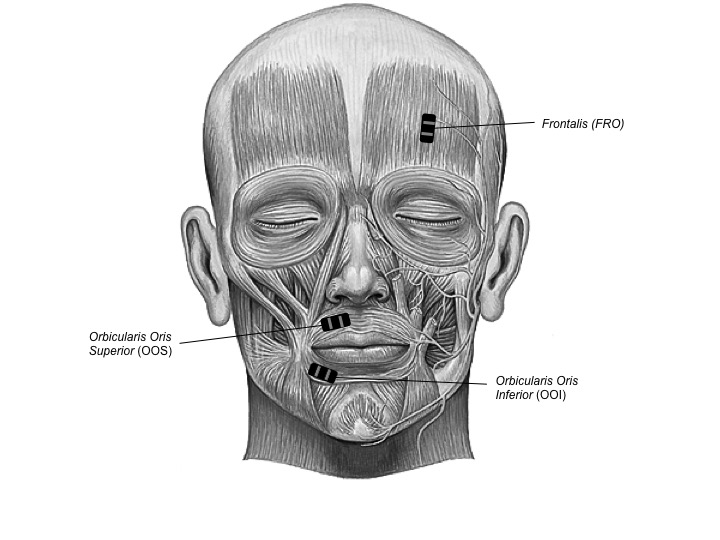
\includegraphics[width=0.75\linewidth]{assets/face_emg} 

}

\caption{Facial muscles of interest. Two speech-related labial muscles: \textit{orbicularis oris superior} (OOS) and \textit{orbicularis oris inferior} (OOI); as well as one non speech-related but sadness-related facial muscle: \textit{frontalis} (FRO).}\label{fig:emgface}
\end{figure}

\hypertarget{procedure}{%
\subsection{Procedure}\label{procedure}}

This study consisted of two parts. The first part was carried out a week before the EMG experiment and consisted in checking the inclusion criteria. We checked that participants did not exceed a threshold on a depressive symptoms scale. This was assessed using the French version of the \emph{Center for Epidemiologic Studies Depression} scale (CES-D, Fuhrer \& Rouillon, \protect\hyperlink{ref-fuhrer_version_1989}{1989}), which evaluates the level of depressive symptom in subclinical population. We also collected information about any potential speech, neurologic, neuromuscular or cardiac disorders and about academic curriculum. Finally, the tendency to ruminate (i.e., trait rumination) in daily life was evaluated using the French version of the Mini-CERTS (Cambridge-Exeter Repetitive Thought Scale, Douilliez et al., \protect\hyperlink{ref-Douilliez2012}{2012}). The second part included two EMG interdependent experiments related to \emph{Rumination Induction} and \emph{Rumination Reduction by Muscle Relaxation}. Specifically, Experiment 1 consisted of acquiring physiological EMG data during rest and induced rumination and Experiment 2 consisted of acquiring physiological EMG data after different kinds of relaxation (see below).

During both Experiment 1 and Experiment 2, momentary rumination was assessed using four different Visual Analogue Scales (VAS, the first two being adapted and translated to French from Huffziger et al., \protect\hyperlink{ref-Huffziger2012}{2012}) rated from 0 to 100: i) \enquote{At this moment, I am thinking about my feelings} (referred to as VAS \enquote{\emph{Feelings}}), ii) \enquote{At this moment, I am thinking about my problems} (referred to as VAS \enquote{\emph{Problems}}), iii) \enquote{At this moment, I am brooding about negative things} (referred to as VAS \enquote{\emph{Brooding}}) and iv) \enquote{At this moment, I am focused on myself} (referred to as VAS \enquote{\emph{Focused}}).

\hypertarget{experiment-1-rumination-induction}{%
\subsubsection{Experiment 1: rumination induction}\label{experiment-1-rumination-induction}}

Participants were seated in front of a computer screen in a comfortable and quiet room. EMG sensors were positioned as explained above (see Figure \ref{fig:emgface}). Before the rumination induction, each participant underwent a non-specific relaxation session (i.e., without targeting specific muscles) in order to minimize inter-individual initial thymic variability (approximate duration ∼330 s). Immediately after, participants were instructed to remain silent and not to move for one minute to carry out EMG \enquote{baseline} measurements. Then, participants' initial level of rumination was assessed using the four VASs.

Subsequently, participants were invited to perform a 15-min I.Q. test, which was presented on the computer screen facing them. They were instructed to correctly respond to three types of I.Q. questions (logical, mathematical and spatial-reasoning questions) in a very short time (30 s). Most of the questions were very difficult, if not impossible, to correctly answer in 30 s. We included ten different questions for each of the three types of I.Q. question: ten logical questions (e.g., finding the next number of a Fibonacci sequence), ten mathematical questions (e.g., \enquote{What is the result of the following calculus: (30/165) − (70/ 66)}) and ten spatial-reasoning questions (e.g., finding the next figure of a series). Forced-failure tasks have extensively been employed in the literature to induce a slightly negative mood, ideal for subsequent rumination induction (e.g., Lemoult \& Joormann, \protect\hyperlink{ref-Lemoult2014}{2014}; van Randenborgh, Hüffmeier, LeMoult, \& Joormann, \protect\hyperlink{ref-VanRandenborgh2010}{2010}).

After the I.Q. test, participants were invited to reflect upon the causes and consequences of their feelings, during five minutes (rumination induction). This method is based on the induction paradigm developed by Nolen-Hoeksema \& Morrow (\protect\hyperlink{ref-nolen-hoeksema_effects_1993}{1993}). The classical paradigm uses a series of prompts. In order to avoid the potential confound in muscle activity induced by silent reading, we did not use the full paradigm. We simply summarised the series of prompts by one typical induction sentence. During this period, participants were asked to remain silent and not to move, while EMG recordings were carried out (i.e., EMG Post-induction measures). EMG signals of rumination were collected during the last minute of this period. Finally, participants were instructed to self-report momentary rumination on the four VASs.

\hypertarget{experiment-2-rumination-reduction-by-relaxation}{%
\subsubsection{Experiment 2: rumination reduction by relaxation}\label{experiment-2-rumination-reduction-by-relaxation}}

After Experiment 1, participants were randomly allocated to one of three groups. In the first group, participants listened to a pre-recorded relaxation session that was focused on orofacial speech-related muscles (\enquote{\emph{Orofacial Relaxation}} condition). In the second group, relaxation was focused on the arm muscles (\enquote{\emph{Arm Relaxation}} condition). In the third group, participants simply listened to a story, read by the same person, for an equivalent duration (\enquote{\emph{Story}} condition, detailed content of the story can be found in the \protect\hyperlink{suppCH3}{supplementary materials}, in French). In summary, the first condition allowed us to evaluate the effects of targeted speech muscle relaxation on rumination. The second condition allowed evaluating the effects of a non-orofacial relaxation (i.e., speech-unrelated muscles) while the third condition allowed controlling for effects of attentional distraction during relaxation listening.

The speeches associated with the three conditions, relaxation sessions and story listening session, were delivered to the participants through loudspeakers. They were recorded by a professional sophrology therapist in an anechoic room at GIPSA-lab (Grenoble, France) and were approximately of the same duration (around 330 s).

After the relaxation/distraction session, participants were asked to remain silent and not to move during one minute, during which EMG measurements were collected (EMG Post-relaxation measures). Finally, participants were instructed to self-report rumination on the four VASs.

\hypertarget{data-processing-and-analysis}{%
\subsection{Data processing and analysis}\label{data-processing-and-analysis}}

\hypertarget{emg-data-processing}{%
\subsubsection{EMG data processing}\label{emg-data-processing}}

EMG signal pre-processing was carried out using Labchart 8. The EMG data were high-pass filtered using a Finite Impulse Response (FIR) filter at a cut-off of 20 Hz, using the Kaiser window method with \(\beta\) = 6. Then, output of this first filter was to a low-pass filtered at a cut-off of 450 Hz (with the same parameters), in order to focus on the 20--450 Hz frequency band, following current recommendations for facial EMG studies (Boxtel, \protect\hyperlink{ref-boxtel_optimal_2001}{2001}; De Luca, \protect\hyperlink{ref-de_luca_use_1997}{1997}; De Luca, Donald Gilmore, Kuznetsov, \& Roy, \protect\hyperlink{ref-de_luca_filtering_2010}{2010}).

Although we specifically asked participants to remain silent and not to move during EMG data collection, tiny facial movements (such as biting one's lips) or vocal productions sometimes occurred. Periods with such facial movement or vocal production were excluded from the analysis. To do this, visual inspection of audio, video, and EMG signal was performed. Specifically, for the EMG signals, we compared two methods of signal selection. The first one consisted of setting a threshold on the absolute value of the EMG signal and portions of signals above this threshold were removed. This threshold was empirically chosen using visual inspection of a few samples and set to the mean EMG value plus 6 SDs. The second method consisted of manually removing periods of time that included visually obvious bursts of EMG activity, corresponding to overt contraction (as in Rapin et al., \protect\hyperlink{ref-rapin_emg_2013}{2013}\protect\hyperlink{ref-rapin_emg_2013}{a}). Based on samples from a few participants, the comparisons between these two methods showed that the automatic threshold method was somewhat less sensitive to overt movements. Therefore, the second method was used, as it was more conservative and less prone to leave data related to irrelevant overt movements.

After pre-processing, EMG data were exported from Labchart software to Matlab r2014a (Version 8.3.0.532, www.mathworks.fr). For each EMG signal, mean values were computed under Matlab, using 200 ms sliding windows. The average of these mean values were calculated for each recording session (baseline, after induction and after relaxation/induction). This provided a score for each muscle of interest (OOS, OOI, FCR, FRO) in each Session (Baseline, Post-Induction, Post-Relaxation) for each participant.\footnote{Because of constraints attributable to the design of our experiment, we were not able to perform conventional control measures (e.g., time of the day, food consumption, sport activity, smoking habits, etc.). Moreover, in our study, periods of signal recording had to be shorter than usual HRV analysis time periods (cf.~methodology section). Although recent studies suggest that \enquote{ultrashort term} HRV analysis seems to correlate quite well with HRV analysis performed on longer periods of time (Brisinda et al., \protect\hyperlink{ref-brisinda_comparison_2013}{2013}; Salahuddin, Cho, Jeong, \& Kim, \protect\hyperlink{ref-Salahuddin2007}{2007}), we cannot exclude that our measurements might be unreliable. For these reasons, we chose not to present HRV results in this report and to focus on EMG results as well as subjective reports of rumination.}

\hypertarget{statistical-analyses}{%
\subsubsection{Statistical analyses}\label{statistical-analyses}}

Absolute EMG values are not meaningful as muscle activation is never null, even in resting conditions, due in part to physiological noise (Tassinary, Cacioppo, \& Vanman, \protect\hyperlink{ref-berntson_skeletomotor_2007}{2007}). In addition, there are inter-individual variations in the amount of EMG activity in the baseline. To normalise for baseline activity across participants, we used a differential measure and expressed EMG amplitude as a percentage of baseline level (Experiment 1) or of post-induction level (Experiment 2).

To model EMG amplitude variations in response to the rumination induction (Experiment 1) and relaxation (Experiment 2), we used a bayesian multivariate regression model with the natural logarithm of the EMG amplitude (expressed in \% of baseline level) as an outcome, in an intercept-only model (in Experiment 1), and using Condition (Orofacial, Arm or Story) as a categorical predictor in Experiment 2. We used the same strategy (two multivariate models) to analyse VAS scores (expressed in relative changes) along the two experiments.

These analyses were conducted using RStudio (RStudio Team, 2018) and the \texttt{brms} package (Bürkner, \protect\hyperlink{ref-R-brms}{2018}), an \texttt{R} implementation of Bayesian multilevel models that employs the probabilistic programming language \texttt{Stan} (Carpenter et al., \protect\hyperlink{ref-carpenter_stan_2017}{2017}). Stan implements gradient-based Markov Chain Monte Carlo (MCMC) algorithms (e.g., Hamiltonian Monte-Carlo), which allow yielding posterior distributions that are straightforward to use for interval estimation around all parameters. Two MCMC simulations (or \enquote{chains}) were run for each model, including 100,000 iterations, a warmup of 10,000 iterations, and a thinning interval of 10. Posterior convergence was assessed examining autocorrelation and trace plots, as well as the Gelman-Rubin statistic. Fixed effects were estimated via the posterior mean and 95\% highest density intervals (HDIs), where an HDI interval is the Bayesian analogue of a classical confidence interval.\footnote{While not suffering from the misunderstandings associated with frequentist confidence intervals (for more details, see for instance Morey et al., \protect\hyperlink{ref-morey_fallacy_2015}{2015}).}

This strategy allowed us to examine posterior probability distribution on each parameter of interest (i.e., effects of session and condition on each response variable). When applicable, we also report evidence ratios (ERs), computed using the hypothesis function of the \texttt{brms} package (Bürkner, \protect\hyperlink{ref-R-brms}{2018}). These evidence ratios are simply the posterior probability under a hypothesis against its alternative (Bürkner, \protect\hyperlink{ref-R-brms}{2018}). We also report summary statistics (mean and HDI) of Cohen's d effect sizes, computed from the posterior samples.

\hypertarget{results}{%
\section{Results}\label{results}}

\hypertarget{experiment-1-rumination-induction-1}{%
\subsection{Experiment 1: rumination induction}\label{experiment-1-rumination-induction-1}}

The evolution of VAS scores (for the four assessed scales: Feelings, Problems, Brooding, and Focused) and EMG (for the four muscles: OOS, OOI, FCR and FRO) activity from baseline to post-induction were examined.

\hypertarget{self-reported-rumination-measures-vas-scores}{%
\subsubsection{Self-reported rumination measures: VAS scores}\label{self-reported-rumination-measures-vas-scores}}

Results for VAS relative changes based on the multivariate models described earlier are shown in the right panel of Figure \ref{fig:resultsemgfig1}. Thereafter, \(\alpha\) represents the mean of the posterior distribution of the intercept. Raw pre- and post-induction scores are provided in the \protect\hyperlink{suppCH3}{supplementary materials}.

Mean VAS score on the Feelings scale was slightly lower after induction (\(\alpha\) = −5.55, 95\% HDI {[}-10.89, −0.24{]}, d = −0.23, 95\% HDI {[}-0.46, −0.01{]}), while Problems score was slightly higher (\(\alpha\) = 3.99, 95\% HDI {[}-2.04, 9.83{]}, d = 0.15, 95\% HDI {[}-0.08, 0.37{]}). We observed a strong increase of the score on the Brooding scale (\(\alpha\) = 14.45, 95\% HDI {[}8.07, 20.72{]}, d = 0.50, 95\% HDI {[}0.26, 0.74{]}), and a strong decrease on the Focused scale (\(\alpha\) = −11.63, 95\% HDI {[}-17, −6.07{]}, d = −0.48, 95\% HDI {[}-0.72, −0.24{]}). As we examined the fit of the intercept-only model, these estimates represent the posterior mean for each muscle.

In the following, we report the mean (indicated by the Greek symbol \(\rho\)) and the 95\% HDI of the posterior distribution on the correlation coefficient (\(\rho\)). Examination of the correlation matrix estimated by the multivariate model revealed no apparent correlation neither between Feelings and Problems scales (\(\rho\) = −0.01, 95\% HDI {[}-0.23, 0.22{]}), nor between Feelings and Brooding (\(\rho\) = 0.08, 95\% HDI {[}-0.15, 0.30{]}). However, we observed a strong positive correlation between Problems and Brooding VASs (\(\rho\) = 0.64, 95\% HDI {[}.49, 0.76{]}), a positive correlation between Feelings and Focused (\(\rho\) = 0.30, 95\% HDI {[}.08, 0.50{]}), and a negative correlation between Problems and Focused (\(\rho\) = −0.30, 95\% HDI {[}-0.49, −0.08{]}), as well as between Brooding and Focused (\(\rho\) = −0.18, 95\% HDI {[}-0.39, 0.05{]}).

\begin{figure}[H]

{\centering 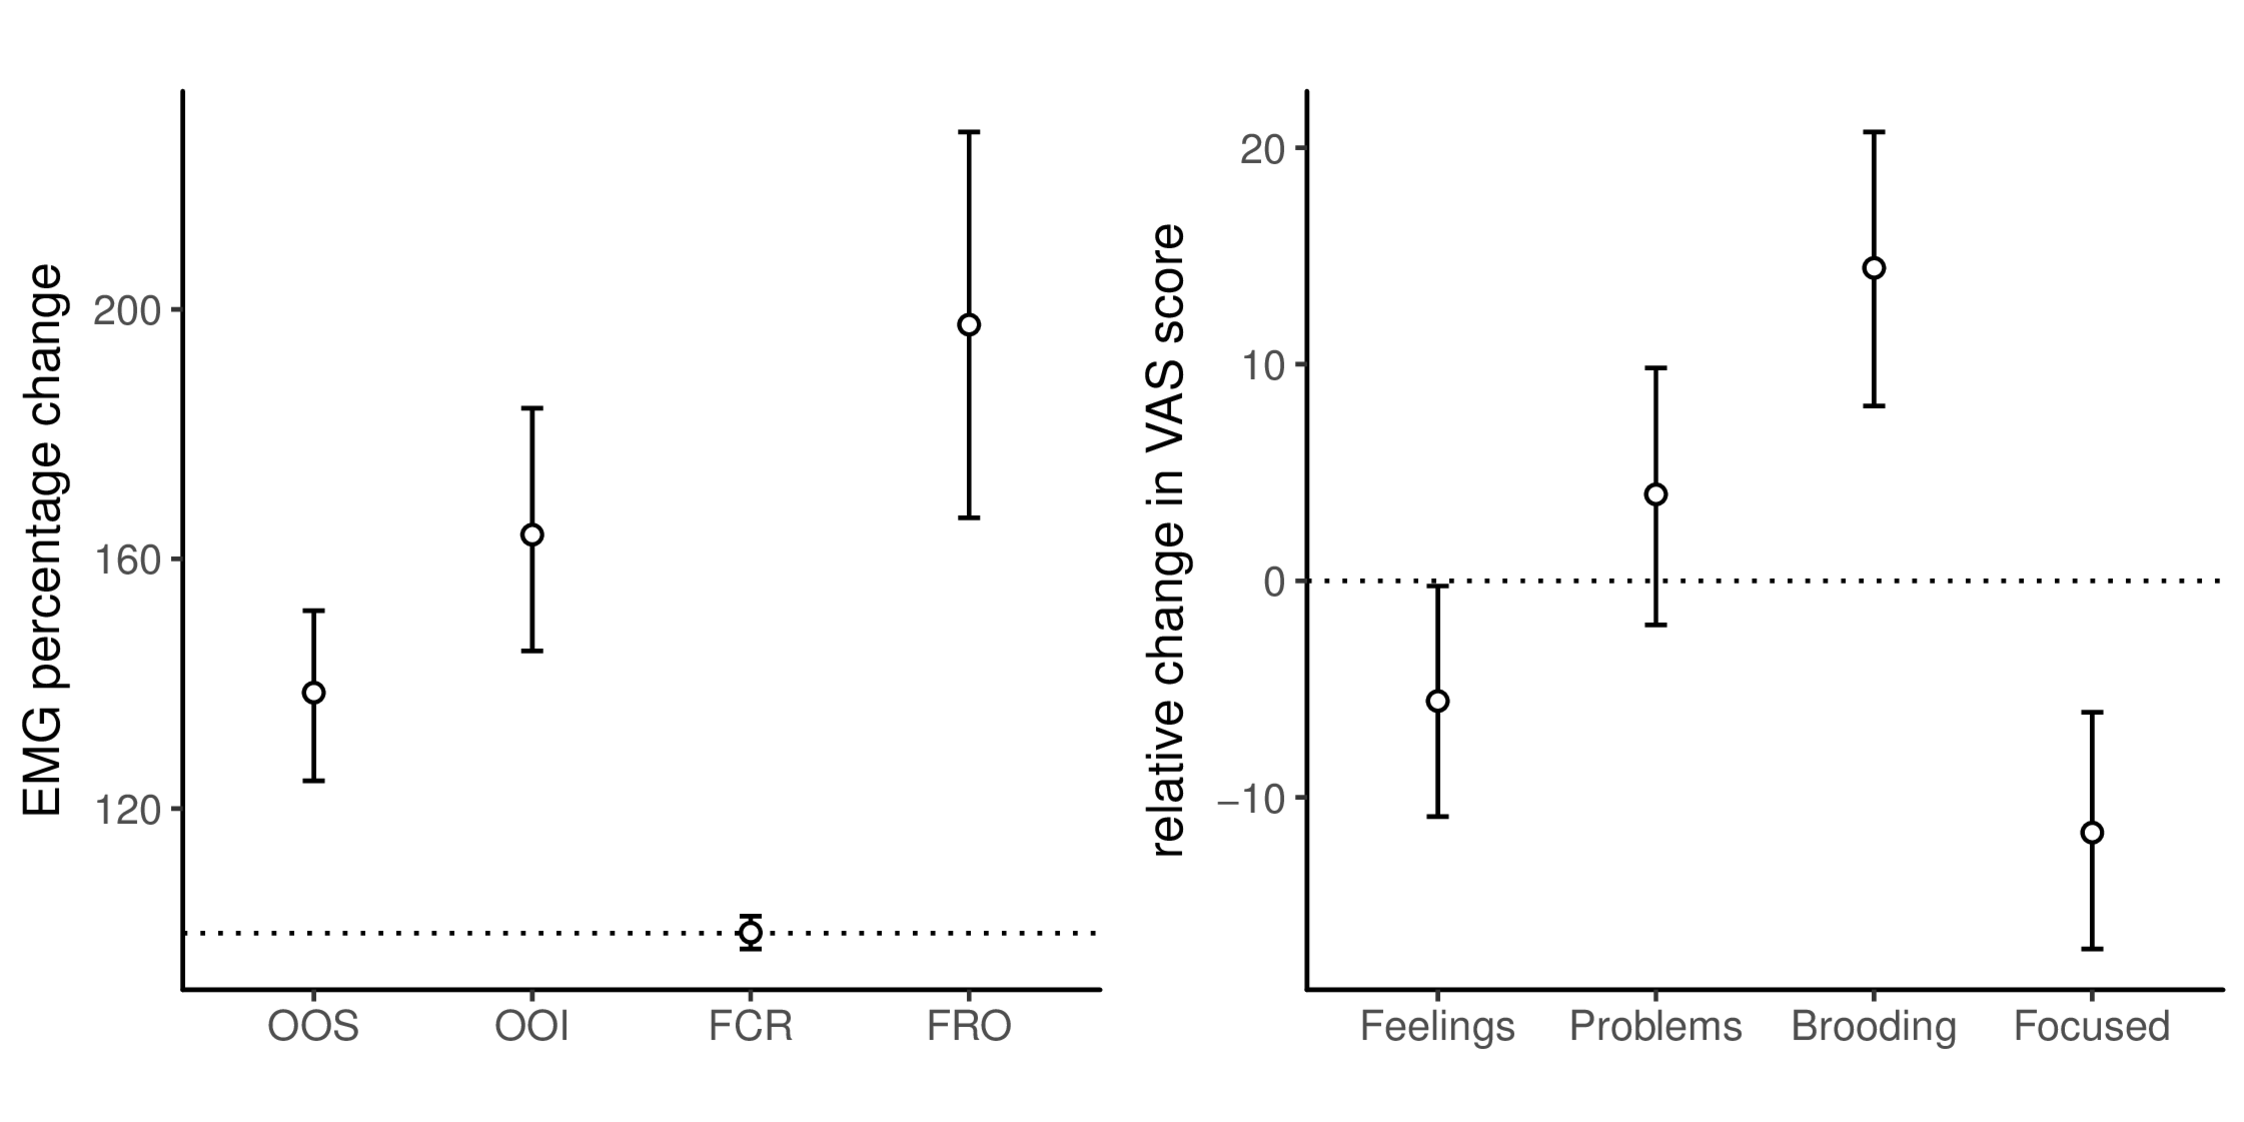
\includegraphics[width=1\linewidth]{assets/emg_fig1} 

}

\caption{Posterior mean (white dots) and 95\% credible intervals for the EMG amplitude (expressed in percentage of baseline level, left panel), and the VAS score (expressed in relative change from baseline, right panel). N = 71 (for each muscle and each VAS). Dashed line represents the null value (i.e., 100\% for the EMG amplitude and 0 for the VAS scores).}\label{fig:resultsemgfig1}
\end{figure}

\hypertarget{emg}{%
\subsubsection{EMG}\label{emg}}

Results for EMG data based on the multivariate model described earlier are shown in the left panel of Figure \ref{fig:resultsemgfig1}. Summary statistics were computed on posterior samples transformed back from log scale.

Mean EMG amplitude for OOS was higher after induction (\(\alpha\) = 138.57, 95\% HDI {[}124.43, 151.71{]}, d = 0.66, 95\% HDI {[}0.49, 0.84{]}) as well as for OOI (\(\alpha\) = 163.89, 95\% HDI {[}145.24, 184.14{]}, d = 0.77, 95\% HDI {[}0.61, 0.94{]}), and FRO (\(\alpha\) = 197.55, 95\% HDI {[}166.59, 228.42{]}, d = 0.74, 95\% HDI {[}0.59, 0.89{]}). Effects on the FCR were approximately null (\(\alpha\) = 100.10, 95\% HDI {[}97.48, 102.76{]}, d = 0.01, 95\% HDI {[}-0.24, 0.23{]}).

Examination of the correlation matrix estimated by the bayesian multivariate model revealed a positive correlation between OOS and OOI EMG amplitudes (\(\rho\) = 0.44, 95\% HDI {[}.24, 0.61{]}), while no apparent correlations neither between OOS and FCR (\(\rho\) = 0.09, 95\% HDI {[}-0.14, 0.31{]}), OOS and FRO (\(\rho\) = 0.12, 95\% HDI {[}-0.11, 0.35{]}), OOI and FCR (\(\rho\) = 0.02, 95\% HDI {[}-0.21, 0.25{]}), FRO and FCR (\(\rho\) = −0.06, 95\% HDI {[}-0.28, 0.17{]}), nor OOI and FRO (\(\rho\) = 0.07, 95\% HDI {[}-0.16, 0.29{]}). Scatterplots, marginal posterior distributions and posterior distributions on correlation coefficients are available in \protect\hyperlink{suppCH3}{supplementary materials}.

In order to check whether the propensity to ruminate could predict the effects of the rumination induction on EMG amplitude, we compared the multivariate model described above, with a similar model but with the score on the abstract dimension of the Mini-CERTS as an additional predictor. We compared these models using the widely applicable information criterion (WAIC; Watanabe, 2010), via the WAIC function of the \texttt{brms} package (Bürkner, \protect\hyperlink{ref-R-brms}{2018}). Results showed that the intercept-only model had a lower WAIC (WAIC = 177.39) than the more complex model (WAIC = 182.01), indicating that there is no predictive benefit in adding the Mini-CERTS score as a predictor.

\hypertarget{correlations-between-emg-amplitudes-and-vas-scores}{%
\subsubsection{Correlations between EMG amplitudes and VAS scores}\label{correlations-between-emg-amplitudes-and-vas-scores}}

Correlations between EMG amplitudes and VAS scores were examined using the \texttt{BayesianFirstAid} package (Bååth, \protect\hyperlink{ref-R-BayesianFirstAid}{2018}), using 15,000 iterations for each correlation coefficient. Both estimated correlation coefficients (\(\rho\)s) and 95\% HDIs are reported in Table \ref{tab:table1}.

\begin{table}[H]
\begin{center}
\begin{threeparttable}
\caption{\label{tab:table1}Estimated correlation coefficients and 95\% HDIs between EMG amplitude evolutions and VAS relative changes.}
\small{
\begin{tabular}{lllll}
\toprule
VAS/Muscle & \multicolumn{1}{c}{OOS} & \multicolumn{1}{c}{OOI} & \multicolumn{1}{c}{FCR} & \multicolumn{1}{c}{FRO}\\
\midrule
Brooding & -0.03 [-0.27, 0.20] & 0.11 [-0.12, 0.34] & -0.26 [-0.47, −0.03] & 0.11 [-0.13, 0.36]\\
Feelings & -0.07 [-0.32, 0.18] & 0.01 [-0.24, 0.25] & -0.20 [-0.43, 0.04] & -0.05 [-0.29, 0.19]\\
Focused & -0.18 [-0.41, 0.06] & -0.26 [-0.47, −0.03] & -0.07 [-0.31, 0.18] & 0.01 [-0.24, 0.26]\\
Problems & 0.11 [-0.14, 0.34] & -0.01 [-0.25, 0.23] & -0.09 [-0.33, 0.15] & 0.26 [0.02, 0.50]\\
\bottomrule
\end{tabular}
}
\end{threeparttable}
\end{center}
\end{table}

\hypertarget{experiment-2-rumination-reduction-by-relaxation-1}{%
\subsection{Experiment 2: rumination reduction by relaxation}\label{experiment-2-rumination-reduction-by-relaxation-1}}

In the second experiment, we aimed at comparing the evolution in EMG activity and VAS scores from post-induction to post-relaxation in three different conditions: Orofacial relaxation, Arm relaxation, and listening to a Story.

\hypertarget{self-reported-rumination-measures-vas-scores-1}{%
\subsubsection{Self-reported rumination measures: VAS scores}\label{self-reported-rumination-measures-vas-scores-1}}

Posterior means and 95\% HDIs of the VAS scores in each condition of experiment 2 are represented in Figure \ref{fig:resultsemgfig2} and Table \ref{tab:table2}.

\begin{table}[H]
\begin{center}
\begin{threeparttable}
\caption{\label{tab:table2}Posterior means and 95\% HDIs for each VAS in each condition.}
\small{
\begin{tabular}{llll}
\toprule
VAS & \multicolumn{1}{c}{Condition} & \multicolumn{1}{c}{β [95\% HDI]} & \multicolumn{1}{c}{d [95\% HDI]}\\
\midrule
Feelings & Orofacial & 7.84 [-0.34, 16.05] & 0.38 [-0.02, 0.80]\\
 & Arm & 4.60 [-3.78, 13] & 0.22 [-0.21, 0.62]\\
 & Story & -5.33 [-13.41, 2.89] & -0.26 [-0.68, 0.12]\\
Problems & Orofacial & −15.24 [-23.89, −6.50] & -0.70 [-1.11, −0.28]\\
 & Arm & -4.23 [-13.15, 4.69] & -0.19 [-0.59, 0.22]\\
 & Story & -9.19 [-17.90, −0.39] & -0.42 [-0.83, −0.02]\\
Brooding & Orofacial & -20.40 [-28.78, −11.97] & -0.97 [-1.41, −0.55]\\
 & Arm & -10.42 [-18.87, −1.93] & -0.50 [-0.90, −0.07]\\
 & Story & -15.16 [-23.48, −6.83] & -0.72 [-1.12, −0.30]\\
Focused & Orofacial & 17.03 [7.37, 20.67] & 0.72 [0.29, 1.14]\\
 & Arm & 11.19 [1.56, 20.89] & 0.48 [0.05, 0.88]\\
 & Story & -14.94 [-24.64, −5.32] & -0.64 [-1.05, −0.22]\\
\bottomrule
\end{tabular}
}
\end{threeparttable}
\end{center}
\end{table}

In order to compare the effects of the two kind of relaxation on the VAS scores, we then used the \texttt{hypothesis()} function of the \texttt{brms} package that allows deriving evidence ratios (ER). These evidence ratios are simply the posterior probability under a hypothesis (e.g., the hypothesis that the Orofacial relaxation session would be more effective in reducing self-reported rumination than the Arm relaxation session) against its alternative (Bürkner, \protect\hyperlink{ref-R-brms}{2018}).

Since the Problems and the Brooding scales seemed to be sensitive markers of rumination (as their scores increased after induction in Experiment 1), our analyses were focused on these two scales.

Concerning the Problems VAS, the decrease observed in the Orofacial condition was more pronounced than in the Arm condition (Est = −11.06, SE = 6.35, ER10 = 22.65), and slightly more pro- nounced compared to the Story condition (Est = −6.05, SE = 6.31, ER10 = 4.98). The observed on the Brooding VAS score in the Orofacial condition was larger than in the Arm condition (Est = −9.98, SE = 6.07, ER10 = 18.85), and slightly more important compared to the Story condition (Est = −5.23, SE = 6.01, ER10 = 4.27).

\begin{figure}[H]

{\centering 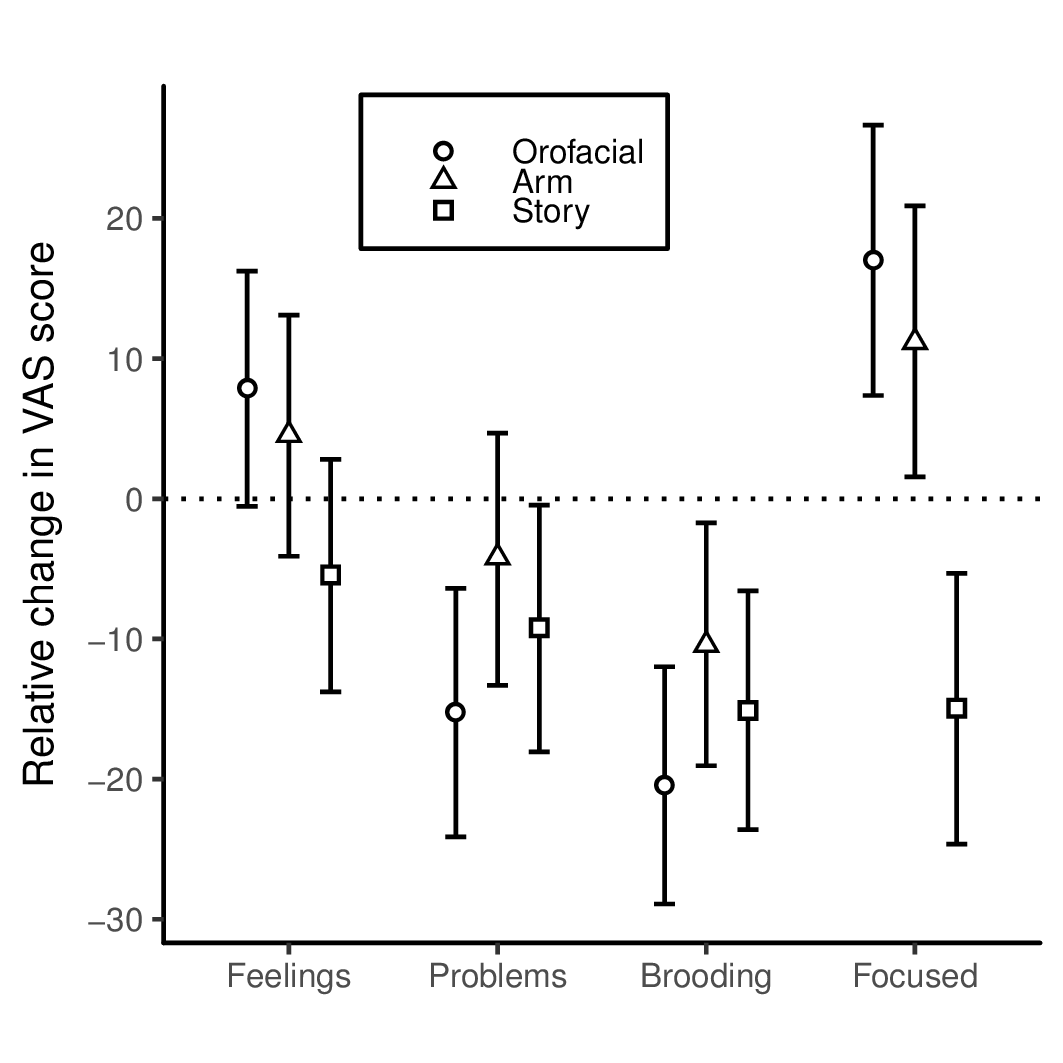
\includegraphics[width=0.75\linewidth]{assets/emg_fig2} 

}

\caption{Posterior mean and 95\% credible intervals for the VAS score (expressed in relative change from post-induction level).}\label{fig:resultsemgfig2}
\end{figure}

\hypertarget{emg-1}{%
\subsubsection{EMG}\label{emg-1}}

Posterior means and 95\% HDIs of the EMG amplitude in each condition of experiment 2 are represented in Figure \ref{fig:resultsemgfig3} and reported in Table \ref{tab:table3}. We used the same strategy as before to compare the effects of the two kinds of relaxation on the EMG amplitudes.

\begin{table}[H]
\begin{center}
\begin{threeparttable}
\caption{\label{tab:table3}Posterior means and 95\% HDIs for each muscle in each condition.}
\small{
\begin{tabular}{llll}
\toprule
Muscle & \multicolumn{1}{c}{Condition} & \multicolumn{1}{c}{β [95\% HDI]} & \multicolumn{1}{c}{d [95\% HDI]}\\
\midrule
OOS & Orofacial & 69.80 [56.96, 83.62] & -0.92 [-1.54, −0.32]\\
 & Arm & 98 [79.83, 117.71] & -0.07 [-0.48, 0.32]\\
 & Story & 109.54 [89.05, 130.74] & 0.16 [-0.21, 0.49]\\
OOI & Orofacial & 71.05 [52.67, 90.71] & -0.62 [-1.24, −0.08]\\
 & Arm & 100.43 [74.05, 128.68] & -0.03 [-0.42, 0.34]\\
 & Story & 89.94 [66.54, 114] & -0.19 [-0.63, 0.22]\\
FCR & Orofacial & 97.01 [93.12, 100.89] & -0.32 [-0.75, 0.10]\\
 & Arm & 98.46 [94.51, 102.48] & -0.16 [-0.58, 0.25]\\
 & Story & 99.24 [95.26, 103.18] & -0.08 [-0.48, 0.32]\\
FRO & Orofacial & 59.22 [48.18, 70.93] & -1.44 [-2.20, −0.70]\\
 & Arm & 61.31 [49.69, 73.82] & -1.32 [-2.08, −0.61]\\
 & Story & 98.31 [80.19, 117.29] & -0.06 [-0.46, 0.32]\\
\bottomrule
\end{tabular}
}
\end{threeparttable}
\end{center}
\end{table}

Concerning the OOS, the observed decrease in the Orofacial condition was more pronounced than in the Arm condition (Est = −0.34, SE = 0.14, ER10 = 140.73), as well as concerning the OOI (Est = −0.35, SE = 0.19, ER10 = 29.46), while we observed no noticeable differences between the two kinds of relaxation concerning the EMG amplitude of the FRO (Est = -0.04, SE = 0.14, ER10 = 1.53).

\begin{figure}[H]

{\centering 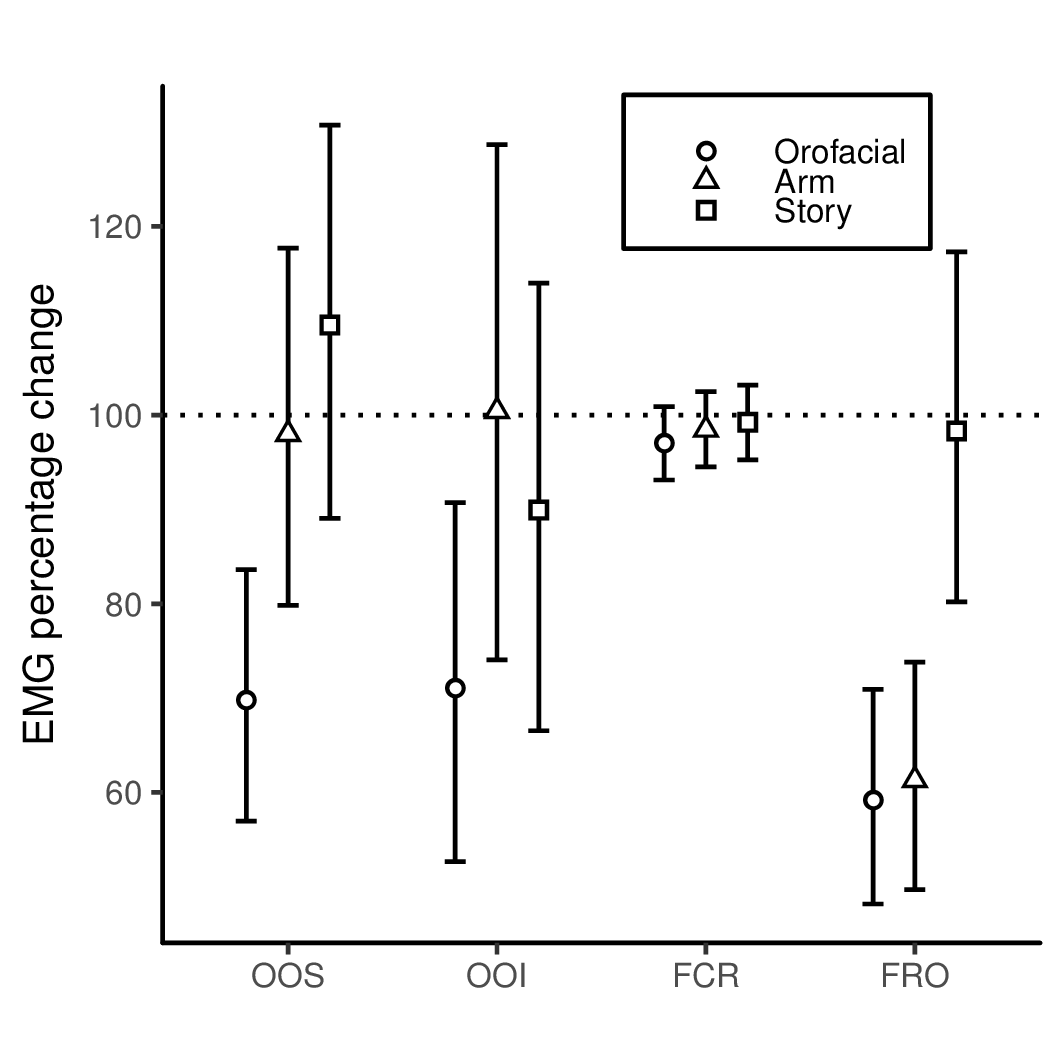
\includegraphics[width=0.75\linewidth]{assets/emg_fig3} 

}

\caption{Posterior mean and 95\% credible intervals for the the EMG amplitude (expressed in percentage of baseline level, left panel).}\label{fig:resultsemgfig3}
\end{figure}

\hypertarget{discussion}{%
\section{Discussion}\label{discussion}}

\hypertarget{experiment-1}{%
\subsection{Experiment 1}\label{experiment-1}}

In the first experiment, we examined electromyographic correlates of induced rumination in healthy individuals. According to the \emph{Motor Simulation view}, we predicted an increase in the activity of all facial muscles after the rumination induction, associated with an increase in self-reported rumination. Alternatively, the \emph{Abstraction view} predicted an increase in self-reported rumination associated with an increase in forehead activity with no changes in either lip or forearm activity.

To test the predictions of these two theoretical views, we compared EMG measures and VAS scores after induction to their values before induction. EMG activity was examined in four muscles: OOS and OOI, two muscles involved in speech production, FRO, a facial negative- affect-related but not speech-related muscle, and FCR, a non-facial control muscle on the non-dominant forearm.

As predicted by the \emph{Motor Simulation view}, we observed an increase in the activity of the two speech-related muscles (OOS \& OOI) as well as in the negative-affect-related muscle (FRO) and no change in FCR activity. The increase in facial EMG together with the increase in the subjective reports of rumination suggests that facial EMG increase is a correlate of verbal rumination. As supported by several studies results, the forehead muscle activity has been associated with unpleasant emotions (Jäncke et al., \protect\hyperlink{ref-Jancke1996}{1996}) or anxiety (Conrad \& Roth, \protect\hyperlink{ref-conrad_muscle_2007}{2007}). The increase in FRO activity observed here is consistent with the increase in negative emotions induced by our negatively valenced induction procedure. \emph{Orbicularis oris} lip muscles are associated with speech production. The increase in lip activity observed here suggests that the speech motor system was involved during the ruminative phase. The fact that the FCR remained stable after rumination induction suggests that the observed facial activity increase was not due to general body tension induced by a negative mental state. These facial EMG results therefore support the hypothesis that rumination is an instance of articulatory-specified inner speech.

After the rumination induction, a larger increase in OOI activity was observed compared to the increase in OOS activity. This finding is consistent with previous findings of higher EMG amplitude in the lower lip during speech and inner speech (e.g., Barlow \& Netsell, \protect\hyperlink{ref-barlow_differential_1986}{1986}; Regalo et al., \protect\hyperlink{ref-regalo_electromyographic_2005}{2005}; Sokolov, \protect\hyperlink{ref-sokolov_inner_1972}{1972}) or auditory verbal hallucinations (Rapin et al., \protect\hyperlink{ref-rapin_emg_2013}{2013}\protect\hyperlink{ref-rapin_emg_2013}{a}). Rapin et al. (\protect\hyperlink{ref-rapin_emg_2013}{2013}\protect\hyperlink{ref-rapin_emg_2013}{a}) have explained the difference between the activities of the two lip muscles by muscle anatomy. The proximity of the OOI muscle with other speech muscles (such as the depressor angular muscle or the mentalis) could increase the surface EMG signal captured on the lower lip (OOI), as compared to the upper lip (OOS) during speech. An even larger increase in FRO activity was observed compared to the increase in lip muscle activity. As EMG amplitude is known to vary with muscle length (Babault et al., \protect\hyperlink{ref-babault_effect_2003}{2003}), the greater increase in frontalis activity could be explained by its anatomical properties.

However, although a functional distinction can be drawn between the forehead and the lip muscles, one should acknowledge the fact that these two sets of muscles can be commonly activated during some behaviours. For instance, van Boxtel \& Jessurun (\protect\hyperlink{ref-van_boxtel_amplitude_1993}{1993}) have shown that orbicularis oris inferior and frontalis were both activated during a two-choice serial reaction task in which nonverbal auditory or visual signals were presented. Moreover, there was a gradual increase in EMG activity in these muscles during the task, either when the task was prolonged or when the task was made more difficult. They interpreted this increase in EMG activity as associated with a growing compensatory effort to keep performance at an adequate level. An alternative interpretation is that the increase in task difficulty was dealt with by inner verbalization. Covertly rehearsing the instructions or covertly qualifying the stimuli might have helped the participants to perform adequately. Therefore, the increase in orbicularis oris activity might have been related to an increase in covert verbalization, whereas the increase in frontalis activity might have been related to increased anxiety or tension. The fact that the EMG increase was muscle specific, and that some facial muscles (\emph{orbicularis oculi}, \emph{zygomaticus major}, \emph{temporalis}) did not show an increase in activity unless the task became too difficult, supports this interpretation. It cannot be ruled out, however, that orbicularis oris activity may in some cases be related to mental effort without mental verbalisation. Nevertheless, although the I.Q. test itself was designed to induce mental effort, no cognitively demanding task was asked to the participant during the period of EMG recording (i.e., approximately four minutes after the end of the test). Although we cannot absolutely exclude that rumination in itself could require cognitive effort, it seems unlikely that mental effort was the main factor of variation.

Scores on the VAS need to be discussed in further detail. We examined which VAS scales were most suitable to capture changes in state rumination to allow focused analyses. Due to the \enquote{pre-baseline} relaxation session, during which participants were asked to concentrate on their body and breathing cycles, participants reported a high level of attentional self-focus at baseline (\enquote{Feelings} and \enquote{Focused} VAS). Because of the high level of self-focused attention at baseline, it is likely that the scores on the \enquote{Feelings} and \enquote{Focused} VAS did not show the expected increase after rumination induction (ceiling effect). The scores on the scales \enquote{Problems} and \enquote{Brooding}, which are more representative of maladaptive rumination, did increase after our rumination induction paradigm, however. Interestingly, the \enquote{Brooding} VAS corresponded to a larger increase and seemed to be more sensitive to rumination induction than the \enquote{Problems} VAS. Given this greater sensibility and the strong positive correlation between the \enquote{Brooding} and the \enquote{Problems} VAS, it thus make sense to consider the \enquote{Brooding} VAS as a better estimate of ruminative state, at least within our paradigm. We will therefore only use this scale to assess rumination in the following.

The fact that we did not observe any association between the propensity to ruminate (as measured by the Mini-CERTS questionnaire) and the effects of the induction is consistent with the results of Rood, Roelofs, Bögels, \& Arntz (\protect\hyperlink{ref-Rood2012}{2012}) who found that the level of trait rumination did not moderate the effects of a rumination induction.

\hypertarget{experiment-2}{%
\subsection{Experiment 2}\label{experiment-2}}

In the second experiment, we studied the effects of two muscle-specific relaxation sessions: Orofacial relaxation and Arm relaxation. We compared their effects to a third control condition (Story), which did not involve the deliberate relaxation of any specific muscle. Our predictions were that a decrease in facial EMG activity should be observed in each condition. If the \emph{Motor Simulation view} is correct, we expected a larger decrease in the activity of all facial muscles in the \enquote{Orofacial relaxation} condition than in the \enquote{Arm relaxation} condition, associated with a larger decrease in self-reported rumination. Additionally, we expected a more pronounced decrease in the two relaxation conditions (orofacial and arm relaxation conditions) than in the control (\enquote{Story}) condition. We also expected no difference between relaxation conditions regarding the change in the forearm muscle activity.

The data indicated a decrease in self-reported rumination (\enquote{Brooding} VAS) in each condition. The \enquote{Orofacial} relaxation condi- tion elicited a slightly larger decrease than the \enquote{Arm relaxation} or the \enquote{Story} condition. However, there was extensive individual variation in response to these conditions. As concerns EMG results, we observed a decrease in OOS and OOI activities in all three conditions but this decrease was more pronounced in the orofacial condition than in the other two conditions. The frontalis activity did not show the same pattern. A similar FRO activity decrease was observed in both the orofacial and the non-orofacial relaxation conditions. Therefore, in Experiment 2, the lip muscles and the forehead muscle follow differential evolutions. A dissociation was observed: whereas both orofacial and arm relaxations resulted in a decrease in forehead activity, only orofacial relaxation was successful at reducing lip activity.

Considering both VAS results and the dissociation in EMG patterns, several interpretations are possible. The first interpretation is that verbal production associated with rumination was more reduced by orofacial muscular relaxation than by non-orofacial relaxation. This interpretation is consistent with the fact that the \enquote{Brooding} VAS was slightly more decreased in this condition compared to the other two. The larger decrease in OOS and OOI amplitude after orofacial relaxa- tion would thus reflect this reduction in verbal production, as hypothesised by the \emph{Motor Simulation view}. The fact that FRO activity displayed a similar decrease in both orofacial and non-orofacial relaxation conditions could suggest that any means of body relaxation (be it orofacial or not) is appropriate to reduce negative affect and can therefore reduce forehead contraction. This suggests that the FRO activity increase presumably reflected negative affect and tension (such as observed in EMG studies on generalised anxiety disorder patients, see Conrad \& Roth, \protect\hyperlink{ref-conrad_muscle_2007}{2007}, for a review).

Alternatively, one could also argue that the larger decrease in lip muscle activity after orofacial relaxation finds a more trivial explana- tion in that it seems obvious to expect that orofacial relaxation will be more efficient to reduce lip muscle contraction than non-orofacial relaxation. Thus, the different impacts of the two relaxation sessions on the lip muscles would not be related to reduced rumination per se but simply to a more anatomically targeted relaxation. However, several observations argue against such an interpretation. The larger decrease in the \enquote{Brooding} VAS in the orofacial relaxation condition compared with the other conditions suggests that the reduction in lip muscle activity is indeed related to the reduction in rumination. Moreover, an interpretation solely based on anatomical links does not explain why FRO activity displayed the same amount of reduction in both relaxation sessions. If reduction in muscle activity was merely related to the effect of facial muscle relaxation, then the decrease in FRO activity should have also been higher in the orofacial relaxation condition than in the other relaxation condition, which was not the case. Therefore the dissociation between forehead and lip patterns of activity, together with the differential effects of the two types of relaxation on subjective rumination reports strongly suggest that different processes underlie the activity of these two sets of muscles. We therefore consider that the first interpretation is more plausible: frontalis activity seems related to overall facial tension due to negative affect whereas lip activity seems to be related to the specific involvement of the speech musculature in rumination. These results thus seem to confirm the interpretation of decreased OOS and OOI activities in the orofacial relaxation condition as markers of rumination reduction.

Interestingly, we observed no changes of forearm EMG activity in any of the three conditions of Experiment 2. The fact that the relaxation session focused on the forearm was not associated with a decrease in FCR activity has a simple explanation: FCR activity had not increased after rumination induction and had remained at floor level. The forearm was thus already relaxed and the Arm relaxation session did not modify FCR activity. Another interesting conclusion related to this absence of modification of forearm activity is that relaxation does not spuriously decrease muscle activity below its resting level. One possible interpretation of the increase in lip EMG after rumination induction could have been that baseline relaxation artificially decreased baseline activity under its resting level. The facts that forearm activity did not decrease after arm-focused relaxation contradicts this interpretation.

Finally, the \enquote{Story} condition was also associated with a decrease in OOI and FRO activities. This could mean that listening to a story reduced rumination to the same extent as relaxation did. However, the discrepancy observed in \enquote{Focused} VAS between the two relaxation conditions on the one hand and the control condition on the other hand, suggests that the EMG decrease observed in the \enquote{Story} condition might be attributable to a different cause than that observed in the two relaxation conditions. Listening to a story could help reducing rumination by shifting attention away from ruminative thoughts. Relaxation sessions could help reducing rumination by shifting attention to the body in a beneficial way.

\hypertarget{general-discussion}{%
\subsection{General discussion}\label{general-discussion}}

We set out two experiments to examine whether rumination involves motor simulation or is better described as linguistically abstract and articulatory impoverished. We used labial, facial, and arm EMG measures to assess potential articulatory correlates of rumination. The patterns of results of our study seem to be in favour of the motor nature of verbal rumination. In Experiment 1, rumination induction was associated with a higher score on the scale \enquote{I am brooding about negative things} which is representative of abstract-analytical rumination, considered as verbal rumination. This maladaptive rumination state was associated with an increase in the activity of two speech-related muscles, without modification of the arm muscle activity, which indicates that rumination involves activity in speech articulatory muscles, specifically. The concurrent increase in forehead muscle activity could be explained by an increase in negative emotions induced by our negatively valenced induction procedure. The results of Experiment 1 therefore show the involvement of the speech musculature during rumination. This is in line with the \emph{Motor simulation view}, according to which inner speech is fully specified at the articulatory level, not just the lexical level.

In Experiment 2, guided relaxation resulted in a decrease in speech muscle activity. In the lip muscles, the activity decrease was stronger after orofacial relaxation than after arm-focused relaxation. In the forehead muscle, however the effect was the same for both types of relaxation. This decrease in speech muscle activity was associated with a decrease in self-reports of rumination and was most pronounced after orofacial relaxation. These findings suggest that a reduction in speech muscle activity could hinder articulatory simulation and thus limit inner speech production and therefore reduce rumination. This interpretation is consistent with the \emph{Motor Simulation view} of inner speech. Brooding-type rumination was also diminished after the arm-focused relaxation as well as after listening to a story, although less than in the orofacial relaxation. This suggests that general relaxation or distraction are also likely to reduce negative rumination. To summarize, experiments 1 and 2 are consistent with the \emph{Motor Simulation view} of inner speech, according to which speech muscle activity is inherent to inner speech production. Experiment 1 shows the involvement of the lip musculature during brooding-type rumination. Experiment 2 suggests that brooding-type rumination could be reduced by blocking or relaxing speech muscles.

These data support the utility of labial EMG as a tool to objectively assess inner speech in a variety of normal and pathological forms. We suggest that this method could be used as a complement to self-report measures, in order to overcome limitation of these measures.

Our results should be interpreted with some limitations in mind. First, our sample consisted exclusively of women. Although this methodological choice makes sense considering the more frequent occurrence of rumination in women, further studies should be conducted to ascertain that our results may generalize to men. Second, in Experiment 1, no between-subject control condition was used to compare with the group of participants who underwent rumination induction. Thus, we cannot rule out that other processes occurred between baseline and rumination induction, influencing responding. Thirdly, substantial inter-individual differences were observed concerning the size of the effect of rumination induction on facial EMG activity. The results of Jäncke (Jäncke, \protect\hyperlink{ref-Jancke1996a}{1996}; Jäncke et al., \protect\hyperlink{ref-Jancke1996}{1996}) can shed light on this last result. Jäncke used a similar procedure (i.e., negative mood induction using a false I.Q. test and facial EMG measurements to assess emotions), except that the experimenter was not in the room while participants performed the test and acknowledged their results. The experimenter then came back to the room and analysed participants' behaviours. Jäncke observed an increase in facial muscular activity (assessed when participants were reading their results) only in partici- pants who were prone to express their distress when the experimenter came back, while more introverted participants did not show any increased facial activity when reading their results. Jäncke interpreted these results in the framework of an ecological theory of facial expression, suggesting that facial expressions would not only be guided by underlying emotions, but also by their communicative properties. Considering these results, it seems likely that the proneness of participants to communicate their emotions could have mediated effects of the induction on their facial EMG activity. This could partially explain the observed inter-individual variability in facial EMG activity associated with rumination. Moreover, even though rumination is a predominantly verbal process, one cannot exclude that some of our participants experienced rumination in another modality (e.g., imagery-based rumination), which would explain their lower than average lip activity.

Thus, a logical next step is to examine qualitative factors that mediate the link between rumination and facial muscular activity. These factors (among others) could be proneness to communicate emotion or proneness to verbalize affects. Additionally, recent studies suggest a link between verbal aptitudes and propensity to ruminate. Uttl, Morin, \& Hamper (\protect\hyperlink{ref-Uttl2011}{2011}) have observed a weak but consistent correlation between the tendency to ruminate and scores on a verbal intelligence test. Penney, Miedema, \& Mazmanian (\protect\hyperlink{ref-Penney2015}{2015}) have observed that verbal intelligence constitutes a unique predictor of rumination severity in chronic anxious patients. To our knowledge, the link between verbal intelligence and induced rumination has never been studied. It would be interesting to examine whether the effects of a rumination induction could be mediated by verbal intelligence, and to what extent this could influence related facial EMG activity.

In conclusion, this study provides new evidence for the facial embodiment of rumination, considered as a particular instance of inner speech. Even if more data are needed to confirm these preliminary conclusions, our results seem to support the \emph{Motor Simulation view} of inner speech production, manifested as verbal rumination. In addition, facial EMG activity provides a useful means to objectively quantify the presence of verbal rumination.

\hypertarget{acknowledgements}{%
\section{Acknowledgements}\label{acknowledgements}}

This project was funded by the ANR project INNERSPEECH. The first author of the manuscript is funded by a fellowship from Université Grenoble Alpes and a grant from the Pôle Grenoble Cognition. We thank Nathalie Vallet for recording the relaxation and distraction sessions. We thank our colleagues from GIPSA-lab: Marion Dohen for her help in the recording of the audio stimuli in the anechoic room at GIPSA-lab, as well as Christophe Savariaux and Coriandre Vilain for their advice in the audio setup associated with the EMG measures. We are also grateful to Rafael Laboissière and Adeline Leclercq Samson for their advice concerning data analysis. We sincerely thank two anonymous reviewers for their critical reading of our manuscript and their many insightful comments and suggestions. Access to the facility of the MSH-Alpes SCREEN platform for conducting research is gratefully acknowledged.

\hypertarget{suppCH3}{%
\section{Supplementary data}\label{suppCH3}}

Supplementary data associated with this article can be found at \url{https://osf.io/882te/}.

\newpage

\begin{vplace}[1]

\begin{summary}{Summary of Chapter\getcurrentref{chapter}}

Rumination is predominantly experienced in the form of repetitive verbal thoughts and can therefore be considered as a particular case of inner speech. According to the \textit{motor simulation view}, inner speech is a kind of motor action, recruiting the speech motor system. In this framework, we predicted an increase in speech muscle activity during rumination as compared to rest. We also predicted increased forehead activity (associated with anxiety) during rumination. We measured electromyographic activity over the orbicularis oris superior and orbicularis oris inferior muscles, over the frontalis as well as over the flexor carpi radialis muscles. Results showed an increased lip and forehead activity after rumination induction as compared to an initial relaxed state, together with increased self-reported levels of rumination. Moreover, our data suggest that orofacial relaxation is more effective in reducing self-reported state rumination than non-orofacial relaxation. Altogether, these results support the hypothesis that verbal rumination involves the speech motor system. However, as the effects of the rumination induction were not compared to another experimental manipulation, it is difficult to conclude with certainty on the \textit{specificity} of these findings. Therefore, in the next study, we manipulate the modality of ruminative thoughs (i.e., verbal vs. non-verbal thoughts) by comparing the EMG correlates of two forms of rumination induction. This comparison should critically reveals whether the EMG correlates observed in this chapter are specific to speech motor processes.

\end{summary}

\end{vplace}

\hypertarget{chap4}{%
\chapter{Dissociating facial electromyographic correlates of visual and verbal induced rumination}\label{chap4}}

\initial{P}revious research shown that mental rumination, considered as a form of repetitive and negative inner speech, is associated with increased facial muscular activity. However, the relation between these muscular activations and the underlying mental processes is still unclear. In this study, we tried to disentangle the facial electromyographic correlates of induced rumination that were related to either i) mechanisms of (inner) speech production or ii) rumination as a state of pondering on negative affects. To this end, we compared two types of rumination induction. The first one was designed to specifically induce rumination in a verbal modality whereas the second one was designed to induce rumination in a visual modality. Following the \emph{motor simulation view} of inner speech production, we hypothesised that the verbal rumination induction should result in higher activity in the speech-related muscles than the non-verbal rumination induction. We also hypothesised that a relaxation focused on the orofacial area should be more efficient in reducing rumination (when experienced in a verbal modality) than a relaxation focused on a non-orofacial area. Our results do not corroborate these hypotheses, as we did not find modality-specific electromygraphic correlates of rumination. Moreover, the two relaxation types were similarly efficient in reducing rumination, whatsoever the rumination modality. We discuss these results in relation with the inner speech literature, and suggest that because rumination is an habitual and automatic form of emotion regulation, it might be considered as a particularly (strongly) internalised form of inner speech.\footnote{This experimental chapter is a working manuscript reformatted for the need of this thesis. Pre-registered protocol, preprint, data, as well as reproducible code and figures are available at: \url{https://osf.io/c9pag/}.}

\hypertarget{introduction-1}{%
\section{Introduction}\label{introduction-1}}

The phenomenon of inner speech has been attracting the attention of the philosophical and scientific communities for a long time. This interest might be explained by the paradox surrounding inner speech: while common to everyone and experienced on a daily basis, it is nevertheless arduous to investigate. However, much can be learned about inner speech by investigating its different forms of expression. Among these forms is rumination, which, for several reasons, will be the focus of this paper. First, although rumination is common in general population (E. R. Watkins et al., \protect\hyperlink{ref-watkins_comparisons_2005}{2005}), it can precede serious mental disorders such as depression, anxiety, eating disorders, or alcohol abuse (for review, see Nolen-Hoeksema et al., \protect\hyperlink{ref-Nolen-Hoeksema2008}{2008}). Therefore, understanding the fundamental nature of rumination have important implications for clinical practise. Second, rumination can be induced and sustained for a relatively long period of time, making it easier to capture than more elusive forms of inner speech. With the aim of further exploring the nature of rumination, we present the results of a procedure designed to induce rumination in different modalities (verbal versus visual imagery) and to investigate its modality-specific electromyographic correlates.

\hypertarget{rumination-its-definition-functions-and-consequences}{%
\subsection{Rumination: its definition, functions and consequences}\label{rumination-its-definition-functions-and-consequences}}

Rumination can be broadly defined as unconstructive repetitive thinking about past events and current mood states (Martin \& Tesser, \protect\hyperlink{ref-Martin}{1996}). This general definition encompasses different conceptualisations that have been proposed during the last decades. Among the most influential frameworks is the \emph{Response Style Theory} (RST, Nolen-Hoeksema, \protect\hyperlink{ref-nolen-hoeksema_responses_1991}{1991}; Nolen-Hoeksema et al., \protect\hyperlink{ref-Nolen-Hoeksema2008}{2008}). Within this theory, rumination is described as a behavioural pattern that is characterised by perseverative, repetitive and passive thoughts. According to the RST, individuals who are experiencing rumination are repetitively focusing on their negative emotional state, on the fact that they are feeling depressed, and on the causes and consequences of their symptoms (Nolen-Hoeksema, \protect\hyperlink{ref-nolen-hoeksema_responses_1991}{1991}). In this framework, rumination is viewed as a type of response to distress or a coping mechanism which involves focusing the attention on oneself and one's current emotional state (Nolen-Hoeksema, \protect\hyperlink{ref-nolen-hoeksema_responses_1991}{1991}). Alloy, Robinson and colleagues (Alloy et al., \protect\hyperlink{ref-alloy_temple-wisconsin_2000}{2000}; Robinson \& Alloy, \protect\hyperlink{ref-Robinson2003}{2003}; Smith \& Alloy, \protect\hyperlink{ref-Smith2009}{2009}) subsequently appended stress-reactive rumination to this theory, suggesting that rumination can also appear following stressful life events and before the presence of negative affect. When conceptualised in this manner, it is presumed that rumination can occur before the start of the depressive mood, whereas rumination, as conceptualised by Nolen-Hoeksema (\protect\hyperlink{ref-nolen-hoeksema_responses_1991}{1991}), happens as a response to depressive mood. Overall, empirical research suggest that negative affect is an essential part of the ruminative thinking process (e.g., Nolen-Hoeksema \& Morrow, \protect\hyperlink{ref-nolen-hoeksema_effects_1993}{1993}).

Based on different factor analyses and more recent models of rumination, a distinction between harmful and helpful sub-types of rumination has been introduced (e.g., Smith \& Alloy, \protect\hyperlink{ref-Smith2009}{2009}; Watkins, \protect\hyperlink{ref-Watkins2008}{2008}). For instance, a distinction has been suggested between brooding and reflection (Treynor et al., \protect\hyperlink{ref-treynor_rumination_2003}{2003}). Brooding relates to morose pondering along with the passive comparison of one's current circumstances and a certain standard. In contrast, ruminative reflection denotes contemplation and engagement in cognitive problem solving as a means to mitigate one's depressive symptoms. In the same vein, Watkins (\protect\hyperlink{ref-Watkins2008}{2008}) proposed a model for differentiating between harmful and helpful forms of repetitive thought. He argued that repetitive thoughts vary along three dimensions -- valence, context and level of construal (abstract versus concrete). By this account, depressive rumination is characterised by an abstract mode of processing that involves thinking about the causes, meaning, and consequences of feelings or events. This abstract-analytic mode is opposed to a more concrete and helpful mode of processing information focused on direct, detailed and concrete experience. The processing mode theory is supported by experimental evidence showing that an abstract-analytical mode of processing is particularly deleterious for mood and cognition (Watkins, \protect\hyperlink{ref-Watkins2008}{2008}).

A certain level of overlap between rumination and related constructs such as intrusive thoughts, obsessions or worry has been recognised (e.g., Olatunji, Naragon-Gainey, \& Wolitzky-Taylor, \protect\hyperlink{ref-olatunji_specificity_2013}{2013}; Smith \& Alloy, \protect\hyperlink{ref-Smith2009}{2009}). Accordingly, rumination and worry have been suggested to represent a particular form of a broader transdiagnostic process coined as \emph{unconstructive repetitive thinking} (Olatunji et al., \protect\hyperlink{ref-olatunji_specificity_2013}{2013}; Watkins, \protect\hyperlink{ref-Watkins2008}{2008}), \emph{perseverative cognition} (Brosschot, Gerin, \& Thayer, \protect\hyperlink{ref-Brosschot2006}{2006}) or \emph{repetitive negative thinking} (Ehring \& Watkins, \protect\hyperlink{ref-ehring_repetitive_2008}{2008}). All forms of thinking gathered under these umbrella terms share a broad involvement of self-focused repetitive thinking about negative and self-relevant topics (De Raedt, Hertel, \& Watkins, \protect\hyperlink{ref-de_raedt_mechanisms_2015}{2015}). However, one the most important and robust delimitation is the one between worry and rumination. On the whole, it is suggested that worry and rumination can be distinguished by their content and by their temporal orientation (Watkins, \protect\hyperlink{ref-Watkins2008}{2008}), but that the \emph{processes} underlying them would be similar. More precisely, whereas worry is focused on problem solving and future events, (depressive) rumination is rather passive and past-oriented (Nolen-Hoeksema et al., \protect\hyperlink{ref-Nolen-Hoeksema2008}{2008}; Smith \& Alloy, \protect\hyperlink{ref-Smith2009}{2009}). There are also findings suggesting that worry is typically more verbal than rumination (Lawrence et al., \protect\hyperlink{ref-lawrence_visual_2018}{2018}), although some studies did not find this difference (Watkins et al., \protect\hyperlink{ref-watkins_comparisons_2005}{2005}).

Having briefly defined the functions and consequences of rumination, we now turn to a discussion of the nature of ruminative thinking, its phenomenological properties as well as how it can be induced and measured in a controlled environment.

\hypertarget{the-nature-of-ruminative-thoughts}{%
\subsection{The nature of ruminative thoughts}\label{the-nature-of-ruminative-thoughts}}

Rumination has sometimes been portrayed as a form of \emph{inner speech} (Perrone-Bertolotti et al., \protect\hyperlink{ref-Perrone-Bertolotti2014}{2014}) due to its predominantly verbal character (Ehring \& Watkins, \protect\hyperlink{ref-ehring_repetitive_2008}{2008}; Goldwin \& Behar, \protect\hyperlink{ref-goldwin_concreteness_2012}{2012}; Goldwin et al., \protect\hyperlink{ref-goldwin_concreteness_2013}{2013}; McLaughlin et al., \protect\hyperlink{ref-mclaughlin_effects_2007}{2007}). In other words, while ruminating, individuals are most often silently talking to themselves. However, what does inner speech precisely entail is still debated (for a recent review, see Lœvenbruck et al., \protect\hyperlink{ref-loevenbruck_cognitive_2018}{2018}). In the present paper, we examine the \emph{motor simulation view} of inner speech production. Under this view, inner speech (content) is proposed to be the result of a soundless mental simulation of overt speech (Jeannerod, \protect\hyperlink{ref-jeannerod_motor_2006}{2006}; Postma \& Noordanus, \protect\hyperlink{ref-postma_production_1996}{1996}). More precisely, inner is conceived as (inhibited) speech motor acts that trigger --via a \emph{simulation} or an \emph{emulation} mechanism-- multimodal sensory percepts (Lœvenbruck et al., \protect\hyperlink{ref-loevenbruck_cognitive_2018}{2018}). This perspective entails that the speech motor system should be involved during inner speech production and that we could record a peripheral residual activity in the speech muscles. This hypothesis has been corroborated by several studies using orofacial surface electromyography (EMG) during tasks that involve inner speech production such as silent recitation, verbal mental imagery or problem solving (Jacobson, \protect\hyperlink{ref-jacobson_electrical_1931}{1931}; Livesay et al., \protect\hyperlink{ref-livesay_covert_1996}{1996}; McGuigan \& Dollins, \protect\hyperlink{ref-mcguigan_patterns_1989}{1989}; Sokolov, \protect\hyperlink{ref-sokolov_inner_1972}{1972}). Overall, these studies show that inner speech production is usually associated with an increased activity of the speech muscles.

We recently conducted a study to examine the facial EMG correlates of rumination (Nalborczyk et al., \protect\hyperlink{ref-nalborczyk_orofacial_2017}{2017}). We have demonstrated that induced rumination is accompanied by an increased facial EMG activity concurrent with increased self-reported levels of state rumination, as compared with an initial relaxed state. This increase in facial EMG activity as a correlate of induced rumination was taken as suggestive evidence that verbal rumination does involve the speech motor system. Furthermore, after a relaxation session focused on the orofacial area, we observed a larger decrease in self-reported state rumination than after non-orofacial (focused on the forearm) relaxation. We interpreted these findings as consistent with the \emph{motor simulation view}. However, we opened the possibility that participants of this study could have been experiencing rumination in other (non-verbal) modalities, such as rumination in visual mental images. Therefore, the present work is in continuity with our previous study, seeking to further investigate the electromyographic correlates of different rumination modalities (i.e., verbal vs.~visual imagery).

Despite being predominantly experienced in a verbal modality, rumination can also be experienced as visual imagery (Goldwin \& Behar, \protect\hyperlink{ref-goldwin_concreteness_2012}{2012}; Newby \& Moulds, \protect\hyperlink{ref-newby_comparison_2012}{2012}; Pearson et al., \protect\hyperlink{ref-pearson_frequency_2008}{2008}). Visual imagery refers to a process during which perceptual information is retrieved from long-term memory, resulting in the experience of \enquote{seeing with the mind's eye} (Ganis et al., \protect\hyperlink{ref-ganis_brain_2004}{2004}). It has been suggested that because rumination is usually past-oriented, it should increase access to (negative) autobiographical memories (Lyubomirsky et al., \protect\hyperlink{ref-Lyubomirsky1998}{1998}). Moreover, because autobiographical memories are often experienced as visual images, rumination should likewise include visual features (Pearson et al., \protect\hyperlink{ref-pearson_frequency_2008}{2008}). Several studies have obtained results that are consistent with this claim. Among a sample of patients who were diagnosed as clinically depressed, a significant majority (94.7\% and more than 70\%) reported that rumination combined verbal and sensory elements, among which visual imagery (Newby \& Moulds, \protect\hyperlink{ref-newby_comparison_2012}{2012}; Pearson et al., \protect\hyperlink{ref-pearson_frequency_2008}{2008}, respectively). When unselected individuals were asked about the quality of their rumination directly while ruminating, 60.53\% of them said they had been experiencing verbal thoughts and 35.92\% mental images (McLaughlin et al., \protect\hyperlink{ref-mclaughlin_effects_2007}{2007}). Another study comparing naturally occurring depressive and anxious thoughts in a non-clinical sample, found that depressive thoughts involved more images than anxious thoughts (Papageorgiou \& Wells, \protect\hyperlink{ref-papageorgiou_process_1999}{1999}). In addition, a recent study demonstrated that a considerable number of people experience depressive cognition in a visual form (Lawrence et al., \protect\hyperlink{ref-lawrence_visual_2018}{2018}). Furthermore, this study showed that individuals with a visual depressive cognitive style reported a similar amount of rumination as individuals with a verbal style. Overall, the existing literature indicates that rumination can have visual features, despite being predominantly verbal.

There are several reasons to think this distinction is of importance. First of all, mental imagery is usually related to a greater cardiovascular activation than verbal thoughts. This is specifically the case in the stressor-focused concrete visual rumination study, for individuals with high trait rumination (Zoccola et al., \protect\hyperlink{ref-zoccola_cardiovascular_2014}{2014}), although a later study found higher heart rate during verbal thoughts (Woody et al., \protect\hyperlink{ref-woody_trait_2015}{2015}). Authors interpreted the obtained data by connecting it with the cognitive avoidance theory (Sibrava \& Borkovec, \protect\hyperlink{ref-davey_cognitive_2006}{2006}). According to this theory, worry, as a primarily linguistic repetitive thought, is an avoidance response whose goal is to restrain aversive images, thus reducing somatic activation and processing of emotions. Similarly, forming negative mental visual images has been shown to lead to a greater increase in anxiety in comparison to forming negative descriptive sentences (Holmes \& Mathews, \protect\hyperlink{ref-holmes_mental_2005}{2005}). Taken together, these findings suggest that different modes of rumination could have different effects on individuals. Furthermore, if rumination also has a visual quality, imagery-based therapeutic methods could also be beneficial (Pearson et al., \protect\hyperlink{ref-pearson_frequency_2008}{2008}). This idea is supported by studies showing the effectiveness of mental imagery in accessing and modifying emotion in therapy (for an overview, see Hackmann \& Holmes, \protect\hyperlink{ref-hackmann_reflecting_2004}{2004}). On the whole, investigating the verbal and visual features of rumination could contribute to sharpen our understanding of the ruminative processes and lead to better-adapted therapeutic strategies.

\hypertarget{inducing-rumination-in-a-controlled-environment}{%
\subsection{Inducing rumination in a controlled environment}\label{inducing-rumination-in-a-controlled-environment}}

Rumination can be operationalised either as a trait, a stable response style of an individual (Nolen-Hoeksema, \protect\hyperlink{ref-nolen-hoeksema_responses_1991}{1991}), or as an ongoing process or a state. When considered as a trait, individual differences in rumination have been mostly investigated by the mean of questionnaires. The most widely used instrument is the Ruminative Responses Scale (RRS) of the Response Styles Questionnaire (RSQ, Nolen-Hoeksema \& Morrow, \protect\hyperlink{ref-nolen-hoeksema_prospective_1991}{1991}). Participants are asked to rate how often they encounter these thoughts or behaviours when feeling sad or depressed. The short version of the RRS questionnaire comprises two scales, reflection and brooding (Treynor et al., \protect\hyperlink{ref-treynor_rumination_2003}{2003}). The psychometric characteristics of this scale as well as its relationship with depressive symptoms have been extensively studied (for a review, see Nolen-Hoeksema et al., \protect\hyperlink{ref-Nolen-Hoeksema2008}{2008}).

However, self-report measures of rumination have several shortcomings. These measurements can be vulnerable to intents and subjectivity of the participants. They rely on the evaluation of past experience and do not focus on the fact that rumination usually arises in the presence of negative emotion. On the opposite, physiological studies of rumination provide data on rumination as it occurs as well as objective data that are less predisposed to subjective influences. Physiological measures also provide an opportunity to explore underlying mechanisms and central processes (Siegle \& Thayer, \protect\hyperlink{ref-papageorgiou_physiological_2003}{2003}). For this purpose, several protocols set to induce rumination have been devised.

Experimental protocols for inducing rumination usually start with provoking negative mood in participants. To this end, some researchers employed sad music (e.g., Conway, Csank, Holm, \& Blake, \protect\hyperlink{ref-conway_assessing_2000}{2000}), asked participants to recall a sad event (e.g., Rood et al., \protect\hyperlink{ref-Rood2012}{2012}), or put participants in stressful and frustrating situations such as an extremely difficult IQ test (e.g., Nalborczyk et al., \protect\hyperlink{ref-nalborczyk_orofacial_2017}{2017}). Another study tried to cause negative feelings by asking participants to give a speech while being evaluated, though the authors concluded that this stressor was rather mild (Zoccola et al., \protect\hyperlink{ref-zoccola_cardiovascular_2014}{2014}). In the following step, rumination is induced. Most studies have employed the rumination induction procedure developed by Nolen-Hoeksema \& Morrow (\protect\hyperlink{ref-nolen-hoeksema_effects_1993}{1993}). Within this protocol, participants are asked to focus on the meanings, causes, and consequences of their current feelings for eight minutes, while being prompted with a series of sentences. Other studies used either a modified version of this protocol (e.g., Nalborczyk et al., \protect\hyperlink{ref-nalborczyk_orofacial_2017}{2017}) or prompts that were self-devised, but still following the same general idea (Rood et al., \protect\hyperlink{ref-Rood2012}{2012}; Zoccola et al., \protect\hyperlink{ref-zoccola_cardiovascular_2014}{2014}). Similarly, in some studies investigating the differences between worry and rumination, participants were given an explanation of what worry or rumination is and were subsequently asked to engage in it (Goldwin \& Behar, \protect\hyperlink{ref-goldwin_concreteness_2012}{2012}; McLaughlin et al., \protect\hyperlink{ref-mclaughlin_effects_2007}{2007}).

Experimental protocols have also used different means for exploring the characteristics of the ongoing process of rumination. In some studies (e.g., Goldwin \& Behar, \protect\hyperlink{ref-goldwin_concreteness_2012}{2012}; McLaughlin et al., \protect\hyperlink{ref-mclaughlin_effects_2007}{2007}), participants were interrupted and asked about the features and/or content of their thoughts. Other studies used questionnaires to measure the features of the ongoing cognition (Makovac et al., \protect\hyperlink{ref-makovac_verbal_2018}{2018}). Among other characteristics, several studies explored how much the ongoing inner experience was verbal and visual, without manipulating rumination modality. In a few studies, however, experimental protocols have been specifically set out to manipulate this aspect of rumination.

Some of the few studies specifically manipulating verbal and visual rumination were carried out by Zoccola and colleagues (Woody et al., \protect\hyperlink{ref-woody_trait_2015}{2015}; Zoccola et al., \protect\hyperlink{ref-zoccola_cardiovascular_2014}{2014}). The verbal or visual form of rumination (or \emph{mentation type} as these authors refer to it) was induced by playing audio tapes that directed participants' thoughts. Prompts were similar in both conditions, differing only in the verbal/visual instruction (\enquote{Recall the speech task using words, phrases, and sentences.} vs.~\enquote{Recall the speech task using pictures and images.}). Participants were subsequently asked to estimate the proportion of verbal thoughts and mental visual images. Although not directly focused on rumination, the task developed by Holmes, Mathews, Mackintosh, \& Dalgleish (\protect\hyperlink{ref-holmes_causal_2008}{2008}) is quite inspiring in designing a protocol for exploring rumination in different modalities. These authors aimed to compare verbal and imagery processing in terms of their differential effects on emotion. They noticed that previous procedures provided verbal descriptions of the events that needed to be processed verbally or visually. The authors argued that with such descriptions, the imagery condition has an additional processing mode in comparison to the. Their proposed solution was to combine pictorial and verbal cues and to ask participants to integrate them into either a sentence or an image.

Finally, it should be noted that in none of the studies in which thinking modality was manipulated, did the participants solely use one type of thought. Even though participants in the imagery group of Zoccola et al. (\protect\hyperlink{ref-zoccola_cardiovascular_2014}{2014}) reported higher levels of mental images in comparison to the participants in the verbal group, the later group also reported a certain level of mental imagery. This is in line with studies showing that rumination includes both verbal and visual components (e.g., Goldwin \& Behar, \protect\hyperlink{ref-goldwin_concreteness_2012}{2012}; McLaughlin et al., \protect\hyperlink{ref-mclaughlin_effects_2007}{2007}), implying that it is not exclusively experienced in one modality. These results are substantiated by a recent study which has shown that participants generate visual images both in cases where they were told to visualise or to verbally think, while they have strong verbal representations only when asked to verbally think (Amit et al., \protect\hyperlink{ref-amit_asymmetrical_2017}{2017}). Amit et al. (\protect\hyperlink{ref-amit_asymmetrical_2017}{2017}) concluded that there is a difference in volitional control of verbal and visual thinking and that people have better control over inner speech than visual thought. Therefore, we will focus on the relative use of a specific mode of thought rather than trying to induce completely verbal or visual thought.

\hypertarget{the-present-study}{%
\subsection{The present study}\label{the-present-study}}

It has been suggested that there is a need of studies that would induce verbal or visual rumination in order to inspect how the experience of rumination in these two modalities could differ (Lawrence et al., \protect\hyperlink{ref-lawrence_visual_2018}{2018}). Furthermore, there has only been one set of studies, to the best of our knowledge, that has employed a protocol for specifically inducing verbal or visual rumination (Woody et al., \protect\hyperlink{ref-woody_trait_2015}{2015}; Zoccola et al., \protect\hyperlink{ref-zoccola_cardiovascular_2014}{2014}). In addition, there were certain shortcomings in this protocol, some of which were highlighted by the authors, such as the stress induction component. To tackle these problems, we extended the study presented in Nalborczyk et al. (\protect\hyperlink{ref-nalborczyk_orofacial_2017}{2017}) by inducing rumination in distinct modalities to compare their electromyographic correlates.

As previously (Nalborczyk et al., \protect\hyperlink{ref-nalborczyk_orofacial_2017}{2017}), we followed two steps in our protocol. First, either verbal or visual rumination was induced in participants by putting them in a stressful situation and subsequently asking them to think about the causes, consequences of their feelings during that situation. Based on the task developed by Holmes et al. (\protect\hyperlink{ref-holmes_causal_2008}{2008}), instructions were presented by combining pictorial and verbal cues. During this period, we tracked changes in the EMG activity of several facial muscles and monitored self-reported levels of state rumination. Second, we compared the effects of two types of relaxation in relation to the modality of ruminative thoughts, on both the EMG amplitude and the self-reported levels of state rumination.

Several hypotheses were drawn based on the existing literature. First, we expected participants in the verbal rumination condition to report a larger proportion of verbal content in their inner experience and a lesser amount of visual content (in comparison to participants in the non-verbal rumination group). Second, with respect to peripheral muscular activity, we expected the activity in the speech muscles to increase by a greater amount in the verbal rumination condition, whereas the change in the non-speech muscles should occur similarly in both conditions, since both conditions are expected to cause negative emotions to a similar extent. Moreover, the control forearm muscle activity should not vary distinctively between conditions. Third, regarding the different types of relaxation, we hypothesised that both orofacial and arm relaxation should cause a slight decrease of state rumination in the verbal condition. Nevertheless, we expected a stronger decrease in the orofacial relaxation condition as compared to the forearm relaxation.

\hypertarget{methods-1}{%
\section{Methods}\label{methods-1}}

In the \emph{Methods} and \emph{Data analysis} sections, we report how we determined our sample size, all data exclusions, all manipulations, and all measures in the study (Simmons, Nelson, \& Simonsohn, \protect\hyperlink{ref-simmons_21_2012}{2012}). A pre-registered version of our protocol can be found online: \url{https://osf.io/c9pag/}.

\hypertarget{participants-1}{%
\subsection{Participants}\label{participants-1}}

Our sample included 85 female participants, ranging in age from 18 to 31 years (M = 19.8823529, SD = 2.0207621). We chose to include only female participants in the present study, for the following three reasons. First, women have been found to engage in rumination more than men (Johnson \& Whisman, \protect\hyperlink{ref-Johnson2013}{2013}). Second, in comparison with men, women have greater visual imagery abilities and report more vivid mental visual images (as reviewed in Lawrence et al., \protect\hyperlink{ref-lawrence_visual_2018}{2018}). Third, the distribution of gender is very unbalanced in Psychology courses. Therefore, it would be practically impossible to have a well-balanced sample with respect to gender. All participants attended undergraduate Psychology programs at Univ. Grenoble Alpes. They were all native speakers of French, had no history of psychiatric or neurological disorders, speech disorders or hearing deficits. Another inclusion criterion was that participants had no depressive symptoms. This was tested at the beginning of the experiment using the Center for Epidemiologic Studies -- Depression scale (CES-D, Radloff, \protect\hyperlink{ref-radloff_ces-d_1977}{1977}). Those participants whose scores overstepped the threshold did not proceed to the main part of the experiment (N = 16). Instead, they were debriefed and received information about places they could turn to for counselling.

Participants were recruited through the university website. They were told that the goal of the study was to test a French adaptation of a novel intelligence test and were, therefore, blind to the actual goal of the study. Participants received course credits for their participation and were fully debriefed at the end of the experiment. Written consent was obtained from each participant and the study received an approval from the local ethical committee (CERNI, Amendement-2018-02-06-23, Avis-2015-03-03-61).

As described in the preregistration form, we used sequential testing to determine the appropriate sample size. More precisely, we recruited participants until reaching either a predetermined level of precision (this procedure is described in Kruschke, \protect\hyperlink{ref-kruschke_doing_2015}{2015}) or the end of the period of time allocated to this experiment (fixed to eight weeks). We first determined a region of practical equivalence (ROPE) and a target precision level on the main effect of interest (i.e., the interaction between the effect of time (baseline versus post-induction, within-subject) and group (verbal rumination versus visual rumination induction, between-subject design), on the EMG amplitude of the OOI muscle). We recruited participants until the 95\% credible interval (the Bayesian analogue of a confidence interval) around the parameter of interest was at least 0.8 times narrower than the ROPE. The ROPE can be defined as the region comprising the effect sizes that we consider as \enquote{null effects} (alternatively, it defines the minimum effect size of interest). We defined the ROPE as {[}-0.1, 0.1{]} on the scale of the normalised and baseline-standardised EMG amplitude. This ROPE has been defined to correspond to a \enquote{null effect} based on previous EMG data we have collected on control muscles (forearm). Then, we defined the target precision as 0.8 times the width of the ROPE, that is: \(0.8 \times 0.2 = 0.16\). We did not reach this threshold within the allocated time. Thus, we ran the study for the full eight weeks (details on the evolution of the estimation precision can be found in the \protect\hyperlink{suppCh4}{supplementary materials}).

\hypertarget{material-1}{%
\subsection{Material}\label{material-1}}

The experimental procedure was developed using the OpenSesame software (Mathôt, Schreij, \& Theeuwes, \protect\hyperlink{ref-mathot_opensesame_2012}{2012}) and stimuli were displayed on a DELL computer screen of size 1280px*720px. TrignoTM Mini wireless sensors (Delsys Inc.) were used for the detection of the surface EMG signals. These sensors consist of a bigger and a smaller box. The smaller box contains two 5x1mm parallel electrode bars with 10mm between them that record bipolar muscle activation. For facial EMG, the small box with electrodes was attached to the face and the bigger box was usually placed on the side of the neck. Concerning the forearm EMG, both boxes were placed on the forearm. Both boxes were attached by double-sided adhesive tape. Before setting the sensors, the skin was cleaned by Nuprep scrubbing gel and by alcohol wipes. Signal acquisition and synchronisation was done using the PowerLab 16/35 (ADInstrument, PL3516) device with a sampling rate of 1926 Hz. In addition to EMG measurements, the audio signal was simultaneously recorded using a C1000S AKG microphone which was placed 20-30 cm away from participant, while the video was recorded using Sony HDR-CX240E camera. These recordings were taken in order to track any vocal or behavioural artefacts during periods of interest (i.e., baseline, rumination and relaxation). Labchart 8 software (ADInstrument, MLU60/8) was used for EMG and audio data collecting and processing.

Our exploration focused on the muscles that have already been found to be activated during covert or overt speech (e.g., Laurent et al., \protect\hyperlink{ref-Laurent2016}{2016}; Maier-Hein, Metze, Schultz, \& Waibel, \protect\hyperlink{ref-maier-hein_session_2005}{2005}; Schultz \& Wand, \protect\hyperlink{ref-schultz_modeling_2010}{2010}). With surface EMG, it is difficult to precisely relate a given skin position to a specific muscle. However, as authors often refer to the facial positions as muscle positions, we will follow this tradition for clarity. Because of their involvement in speech production, bipolar surface EMG electrodes were positioned on the \emph{orbicularis oris inferior} (OOI), the \emph{zygomaticus major} (ZYG) and the neck muscles (NCK). In addition, electrodes were also placed on the \emph{frontalis} (FRO) as an non-speech but emotion-related muscle. Finally, we positioned a sensor on the \emph{flexor carpi radialis} (FCR) to control for general (whole body) muscle contraction.

Speech-related sensors were positioned on the right side of the face whereas the emotion-related (forehead) sensor was positioned on the left side of participants' faces, following studies that found larger movements of the right side of the mouth during speech production (Nicholls \& Searle, \protect\hyperlink{ref-nicholls_asymmetries_2006}{2006}), and more emotional expression on the left side of the face (Nicholls, Ellis, Clement, \& Yoshino, \protect\hyperlink{ref-nicholls_detecting_2004}{2004}). Since participants were asked to use a mouse to provide answers, the forearm sensor was positioned on the non-dominant forearm (that participants did not use to provide the answer).

\hypertarget{procedure-1}{%
\subsection{Procedure}\label{procedure-1}}

We formed two groups based on the modality participants were asked to ruminate in. Hereafter these groups will be referred to as \emph{verbal} and \emph{visual}. Participants were also divided based on the type of relaxation they were listening to, that is, an \emph{orofacial} relaxation, or an \emph{arm} relaxation. As a result, there were four groups in the experiment: \emph{verbal -- orofacial}, \emph{verbal -- arm}, \emph{visual -- orofacial}, and \emph{visual -- arm}.

\hypertarget{trait-questionaires}{%
\subsubsection{Trait questionaires}\label{trait-questionaires}}

After filling the consent form, participants were asked to complete the CES-D (Radloff, \protect\hyperlink{ref-radloff_ces-d_1977}{1977}). Participants also filled out the short version of the Ruminative Response Scale (RRS, Treynor et al., \protect\hyperlink{ref-treynor_rumination_2003}{2003}), adapted and validated in French (Douilliez, Guimpel, Baeyens, \& Philippot, in preparation). These questionnaires were filled in paper format. Once it was determined that they could participate in the study (i.e., that they did not exceed the threshold for depressive symptoms on the CES-D), participants were equipped with the EMG sensors.

\hypertarget{state-questionaires}{%
\subsubsection{State questionaires}\label{state-questionaires}}

Subsequently, a calibration was carried out, making sure that the sensors on each muscle were suitably detecting signals. Participants were then explained the Visual Analogue Scales (VASs) that were used to obtain various self reports throughout the experiment. Specifically, we explained what we meant by: \emph{At this moment, my thoughts are presented in the form of words} (\emph{VAS Verbal}), and \emph{At this moment, my thoughts are presented in the form of visual mental images} (\emph{VAS Visual}). To assess the level of state rumination, we used a French translation of the Brief State Rumination Inventory (BSRI, Marchetti et al., \protect\hyperlink{ref-marchetti_brief_2018}{2018}), composed of eight items also presented as VASs. From that point, the rest of the stimuli were presented on the computer screen and speakers, and the experimenter (blind to the condition) did not interact with the participants anymore.

\hypertarget{baseline-measurements}{%
\subsubsection{Baseline measurements}\label{baseline-measurements}}

Afterwards, participants listened to a guided relaxation (not focused on any specific muscle). The purpose of this relaxation was to minimise inter-individual variability of the initial mood states and to help participants to relax and get used to wearing the EMG sensors. The recording comprised of 240 seconds of guided relaxation, then a pause was made during which participants were told to continue relaxing and the baseline EMG measurements were recorded, after which the guided relaxation continued for another 30 seconds. Following this, participants baseline level of state rumination, verbal and visual level of thoughts were measured using the VASs.

\hypertarget{imagery-training}{%
\subsubsection{Imagery training}\label{imagery-training}}

Next, participants went through a \enquote{lemon training} based on the task proposed by Holmes et al. (\protect\hyperlink{ref-holmes_causal_2008}{2008}). The objective of this training was to show the participants precisely what was meant by \emph{thinking in words} or \emph{thinking in pictures}. The participants in the \emph{verbal} group were asked to combine an image and a word imagining a sentence in their head, whereas participants in the \emph{visual} group were asked to do the same, but only imagining a picture. There were two trials. After doing this task, participants rated how clear (how vivid) their sentence or image was, following which they had to say or describe it out loud. This served as a verification that participants did the task and that they understood it.

\hypertarget{stress-induction}{%
\subsubsection{Stress induction}\label{stress-induction}}

Afterwards, participants took the intelligence test. The test comprised 18 verbal and 18 spatial intelligence questions. It was designed in a way that most (13/18) questions were very difficult while also containing certain (5/18) items that were relatively easy, in order to not demotivate the participants. Participants were instructed to provide their answer within 30 seconds. The number of questions was selected so that even if participants replied very fast, they still encountered around 15 minutes of this frustrating situation. This manipulation has already been shown successful in inducing a negative mood (Nalborczyk et al., \protect\hyperlink{ref-nalborczyk_orofacial_2017}{2017}).

\hypertarget{rumination-induction}{%
\subsubsection{Rumination induction}\label{rumination-induction}}

When the test was done, participants were asked to think about the causes, signification and consequences of their performance during the test and of their current feelings, while their IQ score was being calculated. The participants in the \emph{verbal} group were asked to do this \emph{with their inner voice} and the participants in the \emph{visual} group \emph{using mental visual images}. Following Holmes et al. (\protect\hyperlink{ref-holmes_causal_2008}{2008})'s task, the instructions were presented in written format together with an image showing a person thinking in words (in the \emph{verbal} group) or in pictures (in the \emph{visual} group). When ready, participants pressed the key and a loading sign showed on their screen which lasted for 5 minutes during which participants were expected to ruminate either using inner speech or mental images. When this period was done, participants were again presented with the VASs.

\hypertarget{muscle-specific-relaxation}{%
\subsubsection{Muscle-specific relaxation}\label{muscle-specific-relaxation}}

Finally, participants listened again to a guided relaxation, only this time there were two types of relaxation. One half of verbal and one half of visual group were assigned to an \emph{orofacial relaxation} group and they listened to the relaxation that was focused on the mouth. The other two halves of both groups were randomly assigned to an \emph{arm relaxation} group and they listened to the relaxation concentrated on the arm. Both relaxations had a similar structure with around 270 seconds of guidance, 60 seconds of pause during which the EMG measurements were performed and 25 seconds of relaxation closure. At the very end, participants were asked to write down what they thought was the goal of the experiment and what they were thinking during the score calculation (i.e., the rumination period). The first question served to assess a potential compliance bias insofar as due to the goal of the experiment (i.e., manipulation of the rumination modality), we could not make participants completely blind to the task. The second question served again to check how much participants followed the instruction. At the end of the experiment, participants were given an exhaustive debriefing explaining the goals of the research.

\hypertarget{emg-signal-processing-1}{%
\subsection{EMG signal processing}\label{emg-signal-processing-1}}

Data were collected using Labchart8 and were subsequently exported to Matlab for signal processing (www.mathworks.fr, Matlab r2015a, version 8.5.0.197613). First, a 50Hz frequency comb filter was applied to eliminate excessive power noise. Then, in keeping with the recommendation for facial EMG studies (De Luca et al., \protect\hyperlink{ref-de_luca_filtering_2010}{2010}), a 20 Hz -- 450 Hz bandpass filter was applied, in order to focus on the facial EMG frequency band. The EMG signal was centered to its mean and cut with respect to the three periods of interest (i.e., baseline, rumination and relaxation period), all of which were divided into 5s blocks. These data were then exported to \texttt{R} version 3.5.0 (R Core Team, \protect\hyperlink{ref-R-base}{2018}), where the mean of the absolute signal was calculated for each 5s block. Thus, a score for each muscle, in each period, for each participant was calculated. Absolute EMG values are not meaningful as muscle activation is never null, even in resting conditions, due in part to physiological noise. In addition, there are inter-individual variations in the amount of EMG amplitude in the baseline. To normalise for baseline amplitude across participants, we thus subtracted the EMG amplitude of the baseline to the two periods if interest (i.e., after rumination and after relaxation) and divided it by the variability of the signal at baseline for each muscle and each participant.

Although participants were given the instruction to remain still and to avoid unnecessary movements, there were a lot of subtle movements (e.g., biting the lips). The blocks containing these \emph{artifacts} were removed from the analysis. This was done by inspecting all recordings and manually removing blocks during which there were visually obvious bursts of the EMG amplitude.

\hypertarget{data-analysis}{%
\subsection{Data analysis}\label{data-analysis}}

Statistical analyses were conducted using \texttt{R} version 3.5.0 (R Core Team, \protect\hyperlink{ref-R-base}{2018}), and are reported with the \texttt{papaja} (Aust \& Barth, \protect\hyperlink{ref-R-papaja}{2018}) and \texttt{knitr} (Xie, \protect\hyperlink{ref-R-knitr}{2018}) packages.

To model EMG amplitude variations in response to the rumination induction, we fitted a Bayesian multivariate regression model with the standardised EMG amplitude as an outcome and \emph{Group} as a categorical predictor (contrast-coded). We used the same strategy for modelling the interaction effect between the type of induction and the type of rumination induction\footnote{An introduction to Bayesian statistical modelling is outside the scope of the current paper but the interested reader is referred to Nalborczyk et al. (\protect\hyperlink{ref-nalborczyk_introduction_2019}{2019}\protect\hyperlink{ref-nalborczyk_introduction_2019}{a}), for an introduction to Bayesian multilevel modelling using the \texttt{brms} package.}. These analyses were conducted using the \texttt{brms} package (Bürkner, \protect\hyperlink{ref-R-brms}{2018}), an \texttt{R} implementation of Bayesian multilevel models that employs the probabilistic programming language \texttt{Stan} (Carpenter et al., \protect\hyperlink{ref-carpenter_stan_2017}{2017}).

\texttt{Stan} implements gradient-based Markov Chain Monte Carlo (MCMC) algorithms, which allow yielding posterior distributions that are straightforward to use for interval estimation around all parameters. Four chains were run for each model, including each 10.000 iterations and a warmup of 2.000 iterations. Posterior convergence was assessed examining autocorrelation and trace plots, as well as the Gelman-Rubin statistic. Constant effects estimates were summarised via their posterior mean and 95\% credible interval (CrI), where a credible interval interval can be considered as the Bayesian analogue of a classical confidence interval, except that it can be interpreted in a probabilistic way (contrary to confidence intervals). When applicable, we also report Bayes factors (BFs) computed using the Savage-Dickey method\footnote{This method simply consists in taking the ratio of the posterior density at the point of interest divided by the prior density at that point (Wagenmakers, Lodewyckx, Kuriyal, \& Grasman, \protect\hyperlink{ref-wagenmakers_bayesian_2010}{2010}).}. These BFs can be interpreted as updating factors, from prior knowledge (what we knew before seeing the data) to posterior knowledge (what we know after seeing the data).

\hypertarget{results-1}{%
\section{Results}\label{results-1}}

The results section is divided into two sections investigating the effects of i) the type of rumination induction and ii) the interaction effect between the type of rumination induction and the type of relaxation. Each section is further divided into two subsections reporting either confirmatory (preregistered) or exploratory (non-preregistered) analyses.

\hypertarget{effects-of-the-rumination-induction-and-rumination-modality}{%
\subsection{Effects of the rumination induction and rumination modality}\label{effects-of-the-rumination-induction-and-rumination-modality}}

\hypertarget{descriptive-statistics-and-figures}{%
\subsubsection{Descriptive statistics and figures}\label{descriptive-statistics-and-figures}}

We represent the standardised EMG amplitude during the rumination period for each facial muscle in Figure \ref{fig:ruminationplot}. This figure reveals that the average standardised EMG amplitude was higher than baseline after the rumination induction for both the OOI and FRO muscles, while it was at the baseline level (on average) for the ZYG and lower than baseline for the NCK. Overall, this figures does not show any group (modality-specific) differences (detailed numerical descriptive statistics are reported in the \protect\hyperlink{suppCh4}{supplementary materials}).

\begin{figure}[H]

{\centering 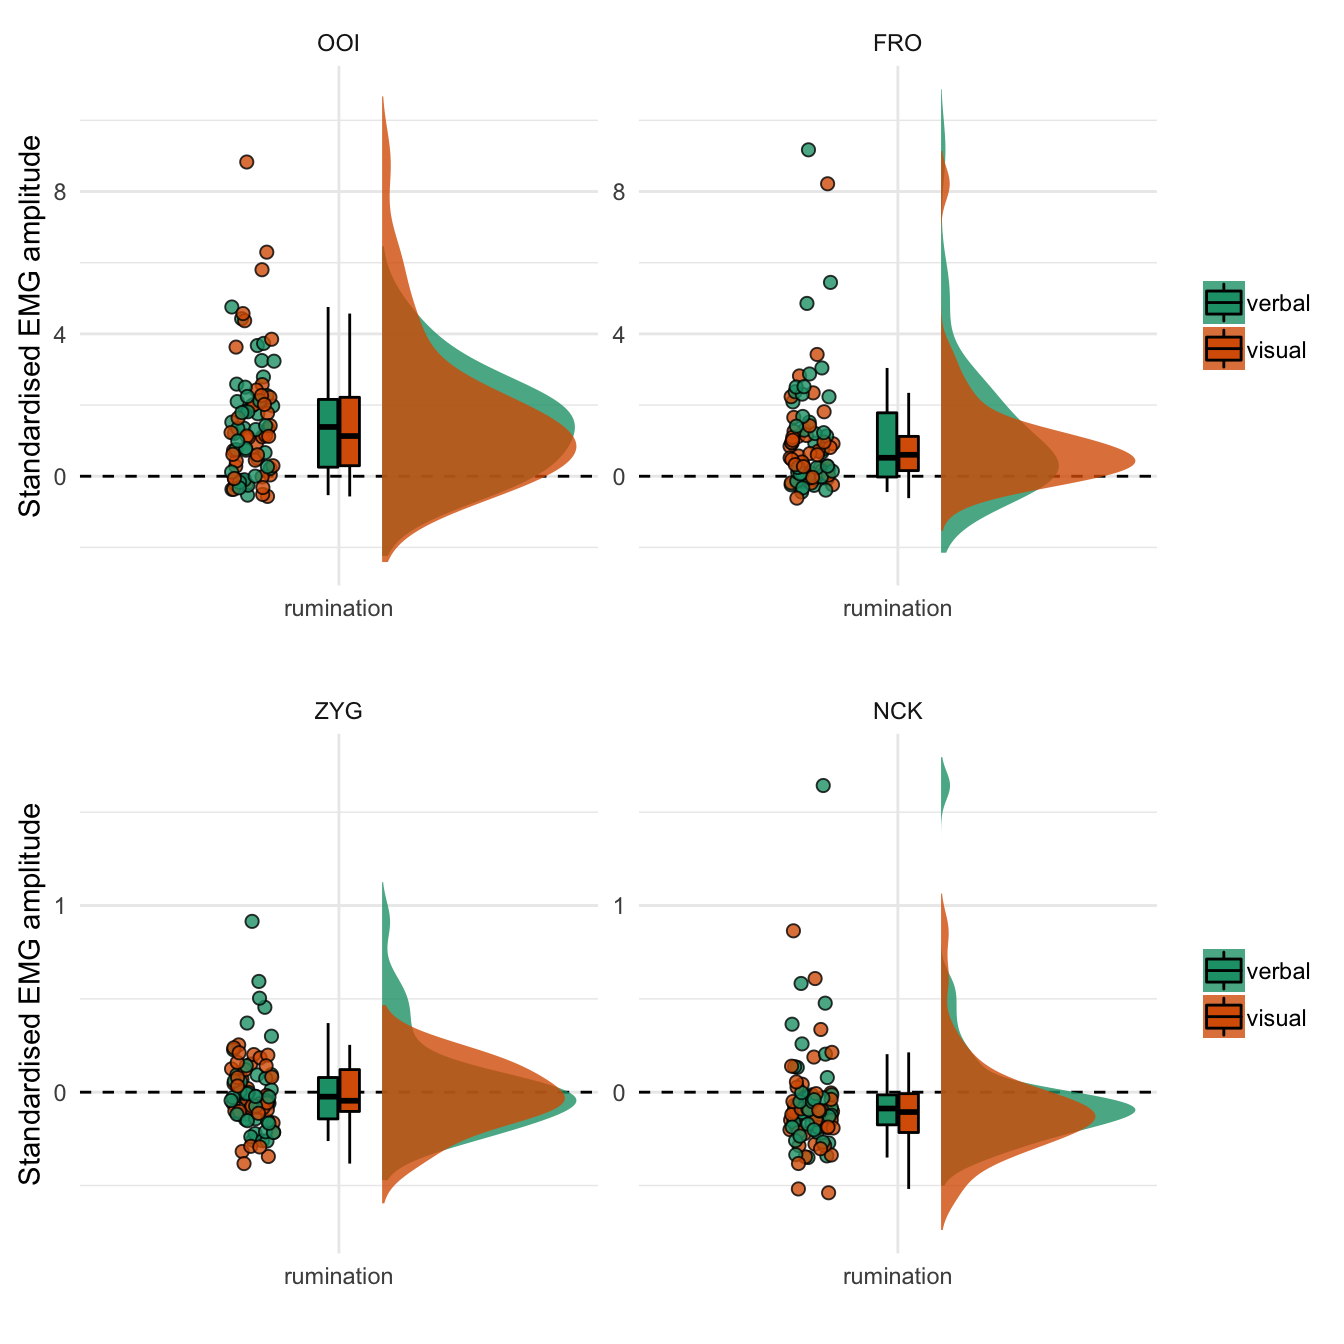
\includegraphics[width=1\linewidth]{04-chap4_files/figure-latex/ruminationplot-1} 

}

\caption{Standardised EMG amplitude during the rumination period. The coloured dots represent the mean standardised EMG amplitude by participant and by type of induction. The boxplot represents the median as well as the first and third quartiles. Note: the y-axis differs between the two rows.}\label{fig:ruminationplot}
\end{figure}

\hypertarget{confirmatory-preregistered-analyses}{%
\subsubsection{Confirmatory (preregistered) analyses}\label{confirmatory-preregistered-analyses}}

In accordance with the preregistered analysis plan, we then fitted a multivariate Gaussian model to estimate the effects of the rumination induction and the difference between the two types of rumination induction. Estimations from this model are reported in Table \ref{tab:outputbmod1}.

\begin{table}[H]
\begin{center}
\begin{threeparttable}
\caption{\label{tab:outputbmod1}Estimates from the multivariate Gaussian model.}
\small{
\begin{tabular}{lccccccc}
\toprule
Response & \multicolumn{1}{c}{Term} & \multicolumn{1}{c}{Estimate} & \multicolumn{1}{c}{SE} & \multicolumn{1}{c}{Lower} & \multicolumn{1}{c}{Upper} & \multicolumn{1}{c}{Rhat} & \multicolumn{1}{c}{BF01}\\
\midrule
ZYG & Intercept & -0.054 & 0.033 & -0.120 & 0.011 & 1.000 & 8.251\\
ZYG & group & 0.065 & 0.066 & -0.066 & 0.193 & 1.000 & 9.332\\
OOI & Intercept & 1.022 & 0.183 & 0.656 & 1.378 & 1.000 & <0.001\\
OOI & group & 0.209 & 0.341 & -0.466 & 0.904 & 1.000 & 2.469\\
NEK & Intercept & -0.002 & 0.023 & -0.050 & 0.043 & 1.000 & 41.497\\
NEK & group & 0.042 & 0.046 & -0.050 & 0.132 & 1.000 & 13.642\\
FRO & Intercept & 1.504 & 0.184 & 1.131 & 1.861 & 1.000 & <0.001\\
FRO & group & -0.178 & 0.346 & -0.869 & 0.516 & 1.000 & 2.535\\
FCR & Intercept & -0.036 & 0.036 & -0.107 & 0.037 & 1.000 & 17.464\\
FCR & group & 0.092 & 0.072 & -0.048 & 0.235 & 1.000 & 6.094\\
\bottomrule
\addlinespace
\end{tabular}
}
\begin{tablenotes}[para]
\textit{Note.} For each muscle (response), the first line represents the estimated average
amplitude after the rumination induction and its standard error (SE). The second line
represents the estimated average difference between the two types of induction (verbal vs. visual). The 'Lower' and 'Upper' columns contain the lower and upper bounds of the 95\% CrI, whereas the 'Rhat' column reports the Gelman-Rubin statistic. The last column reports the BF in favour of the null hypothesis.
\end{tablenotes}
\end{threeparttable}
\end{center}
\end{table}

This analysis revealed that the average EMG amplitude of both the OOI and the FRO muscles was estimated to be higher than baseline (the standardised score was above zero) after rumination induction. However, it was not the case for the ZYG, NCK, and FCR muscles. We did not observe the hypothesised difference according to the type of induction on the OOI (\(\beta\) = 0.209, 95\% CrI {[}-0.466, 0.904{]}, BF\textsubscript{01} = 2.469) nor on the FRO (\(\beta\) = -0.178, 95\% CrI {[}-0.869, 0.516{]}, BF\textsubscript{01} = 2.535).

However, before to proceed further with the interpretation of the results, it is essential to check the validity of this first model. A useful diagnostic of the model's predictive abilities is known as \emph{posterior predictive checking} (PPC) and consists in comparing observed data to data simulated from the posterior distribution (e.g., Gelman et al., \protect\hyperlink{ref-gelman_bayesian_2013}{2013}). Results from this procedure are represented in Figure \ref{fig:ppcbmod1}.

\begin{figure}[H]

{\centering \includegraphics[width=1\linewidth]{04-chap4_files/figure-latex/ppcbmod1-1} 

}

\caption{Posterior predictive checking for the first model concerning the OOI and FRO muscles. The dark blue line represents the distribution of the raw data while light blue lines are dataset generated from the posterior distribution.}\label{fig:ppcbmod1}
\end{figure}

\hypertarget{exploratory-analyses}{%
\subsubsection{Exploratory analyses}\label{exploratory-analyses}}

The previous figure reveals that this first model fails to generate data that look like the data we have collected. More precisely, the data we have collected look highly right-skewed, especially concerning the OOI. As such, modelling the (conditional) mean of the standardised EMG amplitude is highly sensitive to influential observations, and might not be the best index to evaluate the effects of the type of rumination induction. To improve on this first model, we then assume in the following a Skew-Normal distribution for the response. The Skew-Normal distribution is a generalisation of the Gaussian distribution with three parameters \(\xi\) (xi), \(\omega\) (omega), and \(\alpha\) (alpha) for location, scale, and shape (skewness), respectively. Another limitation of the previous model is that it allocated the same weight to every participant. However, for some participants, we had to remove as much as 95\% of their data (during the manual artefact removal step). Accordingly, these participants should weight less in the estimation of the overall effect. In the following models, we weight the importance of each participant by 1 minus the proportion of signal that was rejected for this participant\footnote{Technically, what is weighted is the contribution of the observation to the \emph{likelihood} function.}. Estimations from this model are reported in Table \ref{tab:outputbmod2}.

\begin{table}[H]
\begin{center}
\begin{threeparttable}
\caption{\label{tab:outputbmod2}Estimates from the multivariate (weighted) Skew-Normal model.}
\small{
\begin{tabular}{lccccccc}
\toprule
Response & \multicolumn{1}{c}{Term} & \multicolumn{1}{c}{Estimate} & \multicolumn{1}{c}{SE} & \multicolumn{1}{c}{Lower} & \multicolumn{1}{c}{Upper} & \multicolumn{1}{c}{Rhat} & \multicolumn{1}{c}{BF01}\\
\midrule
ZYG & Intercept & -0.035 & 0.040 & -0.112 & 0.048 & 1.000 & 16.401\\
ZYG & group & 0.087 & 0.066 & -0.045 & 0.220 & 1.000 & 6.443\\
OOI & Intercept & 1.195 & 0.170 & 0.855 & 1.542 & 1.000 & <0.001\\
OOI & group & -0.073 & 0.247 & -0.565 & 0.450 & 1.000 & 4.013\\
NEK & Intercept & -0.005 & 0.031 & -0.065 & 0.058 & 1.000 & 31.357\\
NEK & group & 0.026 & 0.054 & -0.084 & 0.131 & 1.000 & 16.084\\
FRO & Intercept & 1.537 & 0.210 & 1.133 & 1.968 & 1.000 & <0.001\\
FRO & group & -0.030 & 0.313 & -0.700 & 0.588 & 1.000 & 3.194\\
FCR & Intercept & 0.003 & 0.040 & -0.076 & 0.087 & 1.000 & 24.682\\
FCR & group & 0.111 & 0.071 & -0.026 & 0.257 & 1.000 & 4.109\\
\bottomrule
\addlinespace
\end{tabular}
}
\begin{tablenotes}[para]
\textit{Note.} For each muscle (response), the first line represents the estimated average
amplitude after the rumination induction and its standard error (SE). The second line
represents the estimated average difference between the two types of induction (verbal vs. visual). The 'Lower' and 'Upper' columns contain the lower and upper bounds of the 95\% CrI, whereas the 'Rhat' column reports the Gelman-Rubin statistic. The last column reports the BF in favour of the null hypothesis.
\end{tablenotes}
\end{threeparttable}
\end{center}
\end{table}

This analysis revealed that the average EMG amplitude of both the OOI and the FRO muscles was estimated to be higher than baseline (the standardised score was above zero) after rumination induction. However, it was not the case for the ZYG, NCK and FCR muscles. We did not observe the hypothesised difference according to the type of induction on the OOI (\(\beta\) = -0.073, 95\% CrI {[}-0.565, 0.45{]}, BF\textsubscript{01} = 4.013) nor on the FRO (\(\beta\) = -0.03, 95\% CrI {[}-0.7, 0.588{]}, BF\textsubscript{01} = 3.194). The posterior predictive checks for this model are presented in Figure \ref{fig:ppcbmod2} and indicate that this model seems to better accommodate the specificities of the collected data.

\begin{figure}[H]

{\centering 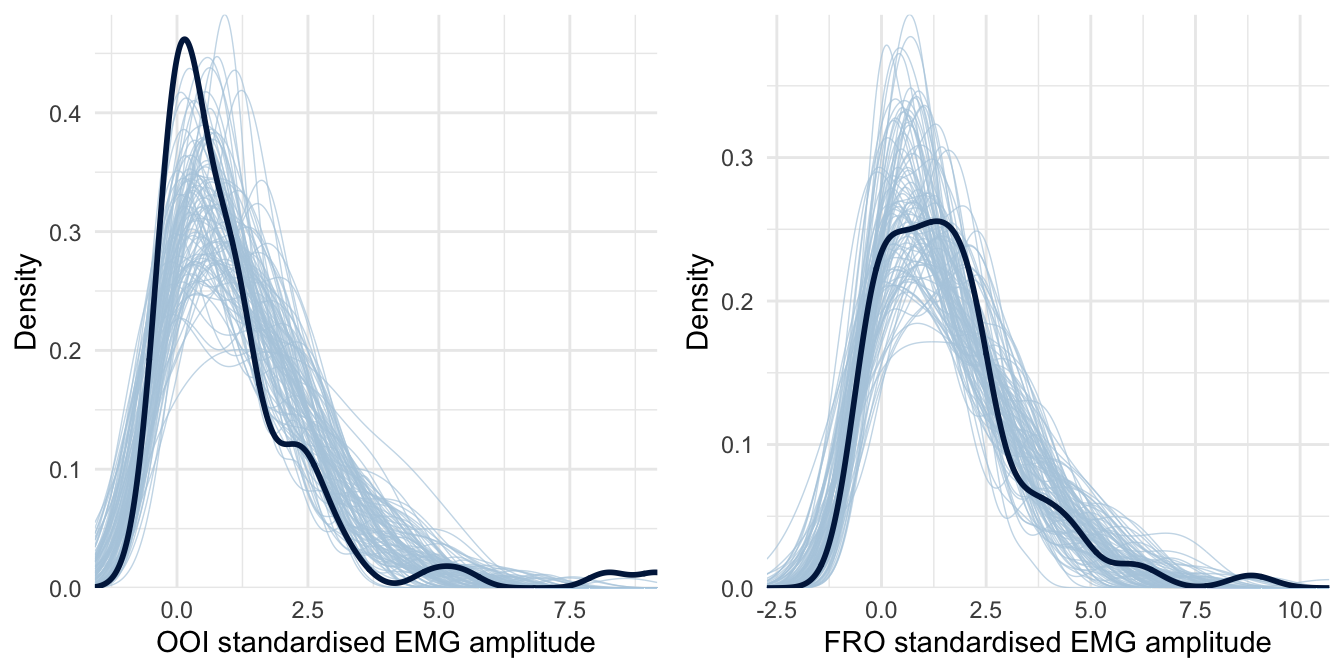
\includegraphics[width=1\linewidth]{04-chap4_files/figure-latex/ppcbmod2-1} 

}

\caption{Posterior predictive checking for the Skew-Normal model concerning the OOI and FRO muscles. The dark blue line represents the distribution of the raw data while light blue lines are dataset generated from the posterior distribution.}\label{fig:ppcbmod2}
\end{figure}

\hypertarget{cluster-analyses}{%
\paragraph{Cluster analyses}\label{cluster-analyses}}

The results of the previous analyses do not corroborate the hypothesis according to which the average EMG amplitude recorded over the speech muscles should be higher in the group that underwent the verbal rumination induction, as compared to the non-verbal rumination induction. However, we might wonder whether the rumination induction was actually efficient in inducing different modalities of ruminative thoughts. To answer this question, we first report the average self-reported levels of either verbal or visual thoughts during the rumination period in Table \ref{tab:verbalvisual}.

\begin{table}[H]
\begin{center}
\begin{threeparttable}
\caption{\label{tab:verbalvisual}Mean and SE of self-reported levels of either verbal or visual thoughts at the end of the rumination period.}
\begin{tabular}{lccc}
\toprule
Group & Verbal VAS & Visual VAS & Sample size\\
\midrule
verbal & 87.45 (2.86) & 31.67 (4.38) & 44\\
visual & 83.92 (4.04) & 30 (4.53) & 41\\
\bottomrule
\end{tabular}
\end{threeparttable}
\end{center}
\end{table}

Considering that both groups showed a similar ratio of verbal/non-verbal thoughts (see Table \ref{tab:verbalvisual}), we used these self-reports to define a posteriori groups of participants that reported more verbal (or non-verbal) ruminations. To this end, we used a cluster analysis (2D k-means) to define two groups (clusters) in the space of the two VASs that have been used to assess the amount of verbal and non-verbal thoughts during the rumination period (see Figure \ref{fig:clusters}).

\begin{figure}[H]

{\centering 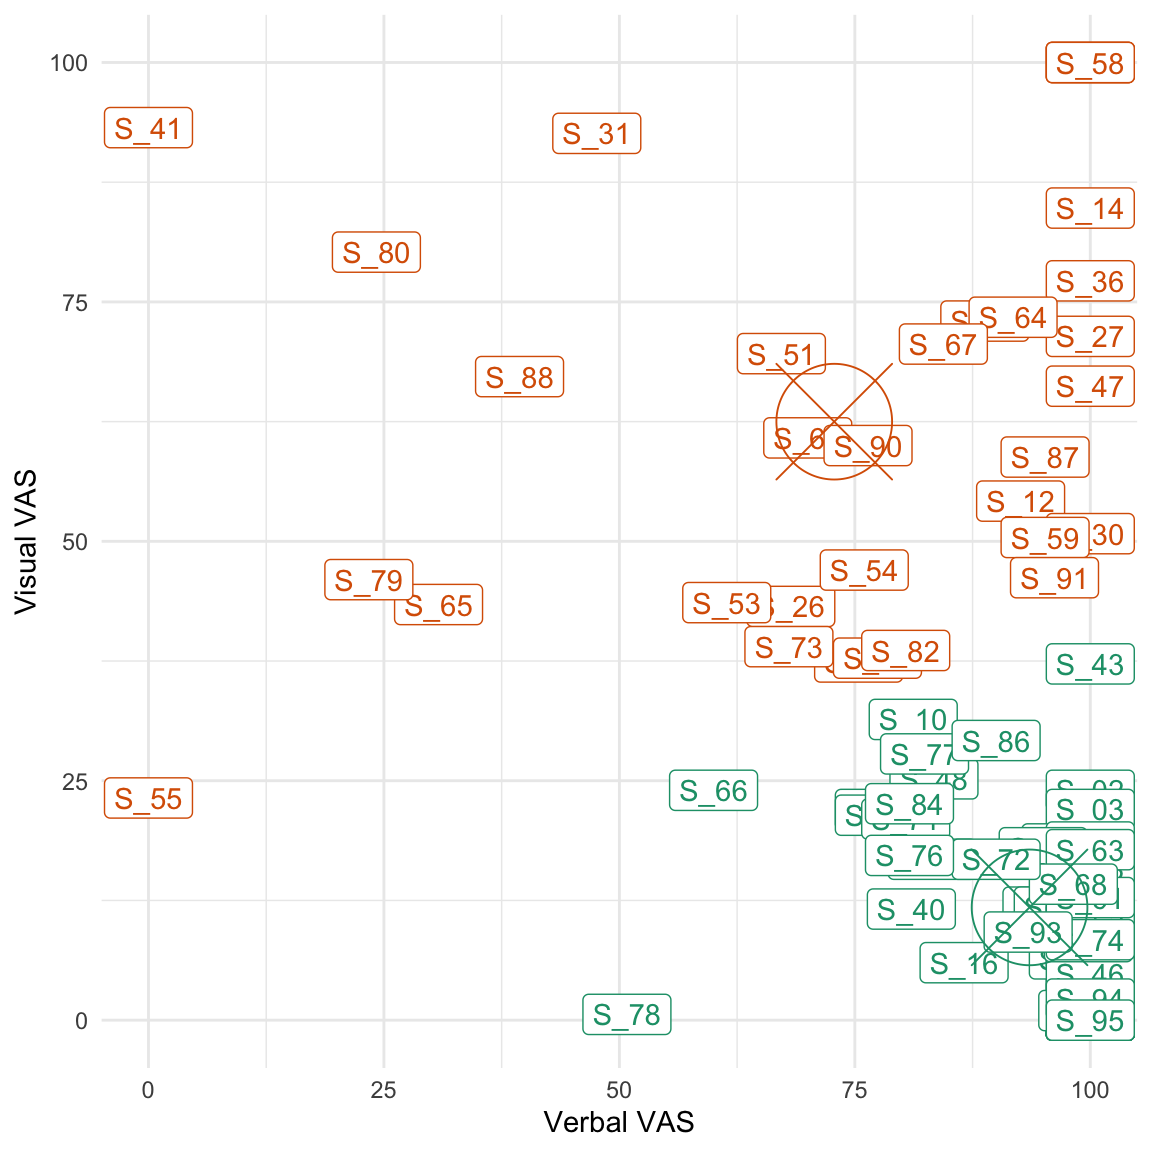
\includegraphics[width=0.75\linewidth]{04-chap4_files/figure-latex/clusters-1} 

}

\caption{Results of the cluster analysis. The centroid of each cluster is represented by a circle and a central cross. The green cluster represents 'verbal ruminators' while the orange one represents 'non-verbal ruminators'.}\label{fig:clusters}
\end{figure}

As can be seen from Figure \ref{fig:clusters} and from Table \ref{tab:clustertable}, this analysis revealed two groups of participants that were either \emph{relatively} i) high on the verbal VAS and low on the visual one or ii) high on the visual VAS and low on the verbal one.

\begin{table}[H]
\begin{center}
\begin{threeparttable}
\caption{\label{tab:clustertable}Center and size (number of participants) of the two clusters identified by the k-means algorithm.}
\begin{tabular}{cccc}
\toprule
Cluster & Verbal VAS & Visual VAS & Size\\
\midrule
1 & 93.55 & 11.77 & 53\\
2 & 72.81 & 62.49 & 32\\
\bottomrule
\end{tabular}
\end{threeparttable}
\end{center}
\end{table}

We then fitted the same model as we previously did but using the cluster (instead of the \enquote{group}) as a predictor to assess the influence of the nature of ruminative thoughts on each muscle' standardised EMG amplitude. Estimations from this model are reported in Table \ref{tab:outputbmod3} and revealed no evidence for a difference between clusters on any muscle (i.e., the \(BF_{01}\) for the effect of \emph{cluster} was superior to 1 for every muscle).

\begin{table}[H]
\begin{center}
\begin{threeparttable}
\caption{\label{tab:outputbmod3}Estimates from the multivariate (weighted) Skew-Normal model based on the k-means clusters.}
\small{
\begin{tabular}{lccccccc}
\toprule
Response & \multicolumn{1}{c}{Term} & \multicolumn{1}{c}{Estimate} & \multicolumn{1}{c}{SE} & \multicolumn{1}{c}{Lower} & \multicolumn{1}{c}{Upper} & \multicolumn{1}{c}{Rhat} & \multicolumn{1}{c}{BF01}\\
\midrule
ZYG & Intercept & -0.032 & 0.041 & -0.110 & 0.053 & 1.000 & 17.005\\
ZYG & cluster & -0.005 & 0.069 & -0.148 & 0.131 & 1.000 & 14.664\\
OOI & Intercept & 1.196 & 0.174 & 0.855 & 1.553 & 1.000 & <0.001\\
OOI & cluster & -0.037 & 0.253 & -0.571 & 0.485 & 1.000 & 3.915\\
NEK & Intercept & 0.004 & 0.031 & -0.056 & 0.066 & 1.000 & 32.501\\
NEK & cluster & -0.071 & 0.052 & -0.177 & 0.037 & 1.000 & 7.382\\
FRO & Intercept & 1.626 & 0.210 & 1.210 & 2.047 & 1.000 & <0.001\\
FRO & cluster & -0.584 & 0.348 & -1.302 & 0.102 & 1.000 & 0.708\\
FCR & Intercept & 0.004 & 0.042 & -0.078 & 0.090 & 1.000 & 24.173\\
FCR & cluster & 0.018 & 0.073 & -0.127 & 0.163 & 1.000 & 13.835\\
\bottomrule
\addlinespace
\end{tabular}
}
\begin{tablenotes}[para]
\textit{Note.} For each muscle (response), the first line represents the estimated average
amplitude after the rumination induction and its standard error (SE). The second line
represents the estimated average difference between the two types of induction (verbal vs. visual). The 'Lower' and 'Upper' columns contain the lower and upper bounds of the 95\% CrI, whereas the 'Rhat' column reports the Gelman-Rubin statistic. The last column reports the BF in favour of the null hypothesis.
\end{tablenotes}
\end{threeparttable}
\end{center}
\end{table}

\hypertarget{relation-between-self-reports-and-emg-amplitude}{%
\paragraph{Relation between self-reports and EMG amplitude}\label{relation-between-self-reports-and-emg-amplitude}}

We represent the relation between self-reported levels of state rumination (after induction) and the EMG amplitude (of the four facial muscles) changes from baseline to post-induction in Figure \ref{fig:selfemg}. This figure reveals an overall positive association between the level of self-reported state rumination after induction and the increase in EMG amplitude from baseline to post-induction on the FRO muscle, but not substantial relation concerning the other muscles.

\begin{figure}[H]

{\centering 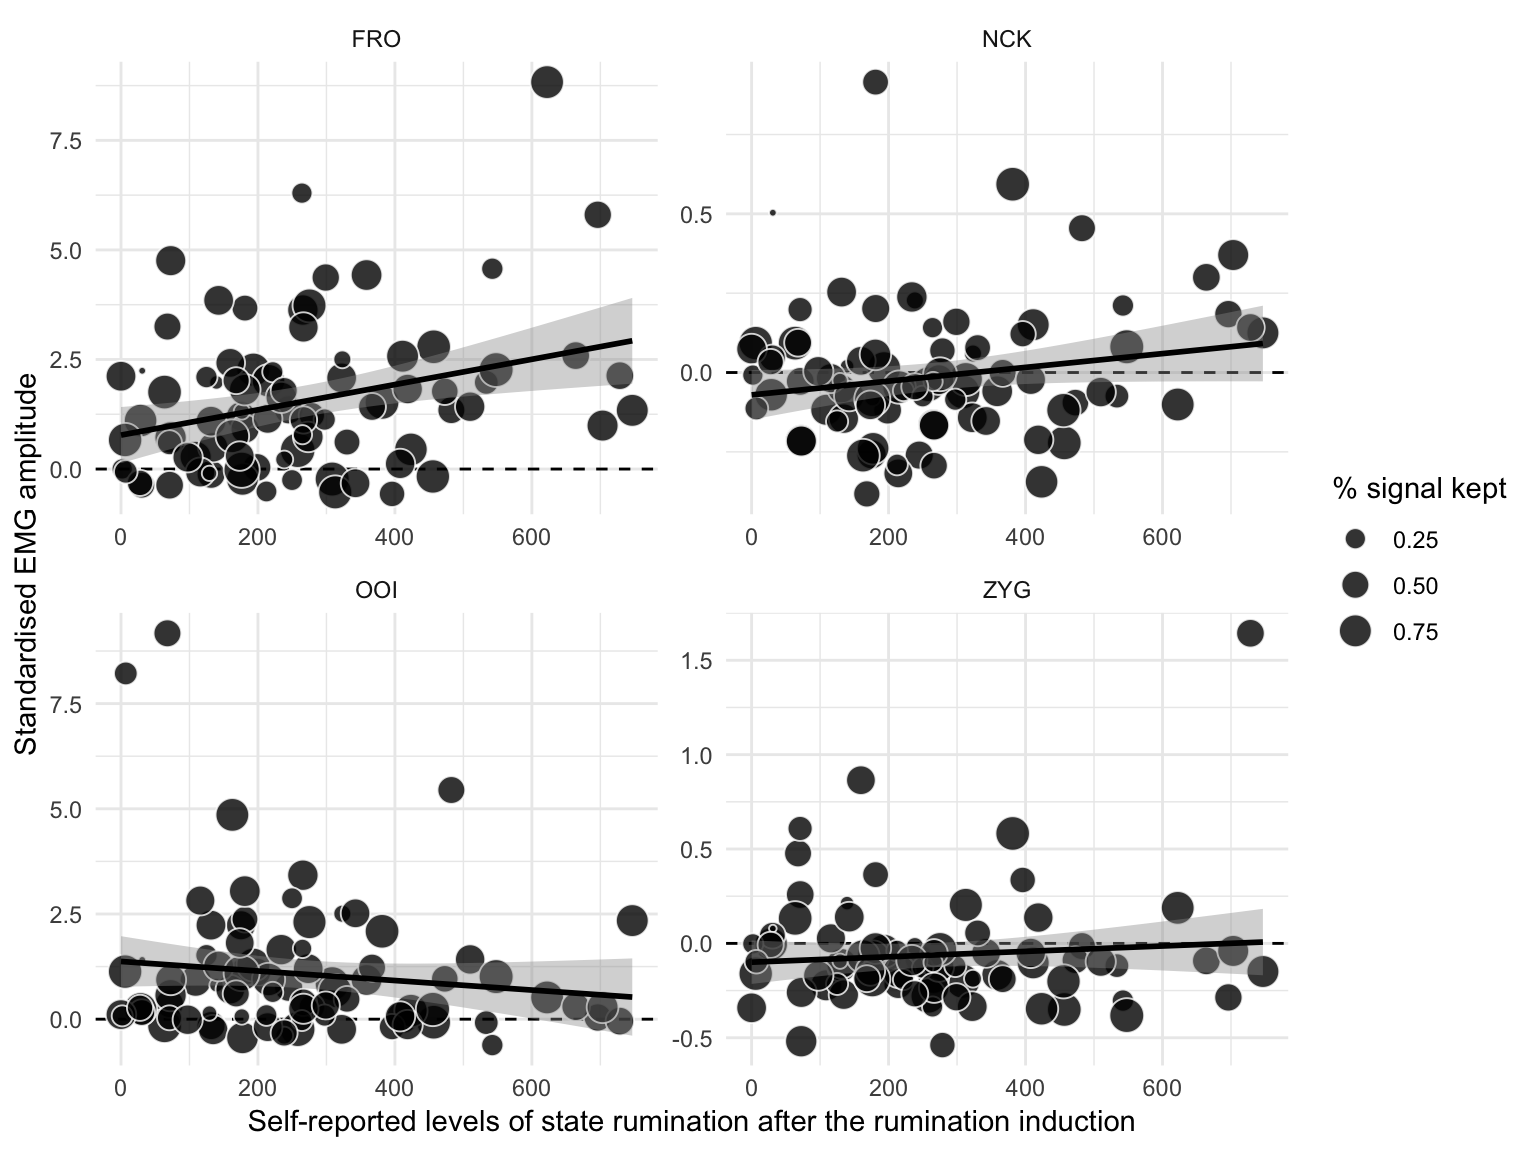
\includegraphics[width=1\linewidth]{04-chap4_files/figure-latex/selfemg-1} 

}

\caption{Relation between self-reported levels of state rumination (on the x-axis) and standardised EMG amplitude after the rumination induction (on the y-axis). The dots represent individual observations, whose size varies with the percentage of signal that was kept after removing artefacts. The black line represents the regression line with its 95\% CI.}\label{fig:selfemg}
\end{figure}

To further analyse the relationship between self-reported levels of state rumination and standardised EMG amplitude, we fitted a weighted multivariate Skew-Normal model (as previously). Estimations from this model are reported in Table \ref{tab:outputbmod4}.

\begin{table}[H]
\begin{center}
\begin{threeparttable}
\caption{\label{tab:outputbmod4}Estimates from the multivariate (weighted) Skew-Normal model assessing the relation between self-reported levels of state rumination and standardised EMG amplitude.}
\small{
\begin{tabular}{lccccccc}
\toprule
Response & \multicolumn{1}{c}{Term} & \multicolumn{1}{c}{Estimate} & \multicolumn{1}{c}{SE} & \multicolumn{1}{c}{Lower} & \multicolumn{1}{c}{Upper} & \multicolumn{1}{c}{Rhat} & \multicolumn{1}{c}{BF01}\\
\midrule
ZYG & Intercept & -0.032 & 0.041 & -0.112 & 0.051 & 1.000 & 17.092\\
ZYG & bsri & 0.004 & 0.034 & -0.061 & 0.070 & 1.000 & 29.882\\
OOI & Intercept & 1.187 & 0.170 & 0.860 & 1.536 & 1.000 & <0.001\\
OOI & bsri & -0.063 & 0.130 & -0.321 & 0.195 & 1.000 & 7.061\\
NEK & Intercept & -0.006 & 0.030 & -0.063 & 0.058 & 1.000 & 33.05\\
NEK & bsri & 0.030 & 0.030 & -0.027 & 0.092 & 1.000 & 19.442\\
FRO & Intercept & 1.523 & 0.208 & 1.126 & 1.957 & 1.000 & <0.001\\
FRO & bsri & 0.283 & 0.192 & -0.097 & 0.660 & 1.000 & 1.805\\
FCR & Intercept & 0.000 & 0.041 & -0.079 & 0.086 & 1.000 & 24.845\\
FCR & bsri & 0.048 & 0.035 & -0.023 & 0.116 & 1.000 & 11.079\\
\bottomrule
\addlinespace
\end{tabular}
}
\begin{tablenotes}[para]
\textit{Note.} For each muscle (response), the first line represents the estimated average
amplitude after the rumination induction and its standard error (SE). The second line
represents the estimated relation between self-reported levels of state rumination and standardised EMG amplitude. As the BSRI scores have been centered and standardised, this estimate approximate a correlation coefficient. The 'Lower' and 'Upper' columns contain the lower and upper bounds of the 95\% CrI, whereas the 'Rhat' column reports the Gelman-Rubin statistic. The last column reports the BF in favour of the null hypothesis.
\end{tablenotes}
\end{threeparttable}
\end{center}
\end{table}

This analysis revealed a weak positive association between self-reported levels of state rumination (BSRI score) after induction and the standardised EMG amplitude recorded over the FRO muscle (\(\beta\) = 0.283, 95\% CrI {[}-0.097, 0.66{]}, BF\textsubscript{01} = 1.805). This analysis revealed no evidence for an association between self-reported levels of state rumination and the standardised EMG amplitude recorded over the other muscles.

In summary, while successful in inducing higher levels of state rumination (higher BSRI scores), the rumination induction did not permit to induce rumination in different modalities. When examining a posteriori groups of verbal vs.~non-verbal ruminators, we did not find evidence for specific electromyographic correlates. Interestingly, we observed a weak positive correlation between self-reported levels of state rumination and the standardised EMG amplitude of the FRO (see \protect\hyperlink{suppCh4}{supplementary materials} for additional analyses).

\hypertarget{effects-of-the-relaxation}{%
\subsection{Effects of the relaxation}\label{effects-of-the-relaxation}}

\hypertarget{planned-preregistered-analyses}{%
\subsubsection{Planned (preregistered) analyses}\label{planned-preregistered-analyses}}

We hypothesised that an orofacial relaxation should cause a stronger decrease of state rumination than a relaxation targeting the arm, for the participants that went through a verbal rumination induction, in comparison to a non-verbal rumination induction. In other words, we expected an interaction effect between the type of rumination induction and the type of relaxation. As the relaxation was directly targeted at the facial muscles, we did not expect the overall EMG amplitude to be a reliable index of ongoing rumination in this part of the experiment. Therefore, we only report an analysis of the self-reported levels of state rumination (but see the \protect\hyperlink{suppCh4}{supplementary materials} for additional analyses).

To analyse this interaction effect, we fitted a Gaussian model with a constant effect of \emph{group} (verbal vs.~non-verbal rumination induction) and \emph{relaxation} (orofacial vs.~arm relaxation) to predict the difference in BSRI score (after minus before the relaxation). Estimations from this model are reported in Table \ref{tab:outputbmod5}.

\begin{table}[H]
\begin{center}
\begin{threeparttable}
\caption{\label{tab:outputbmod5}Estimated changes in self-reported levels of state rumination (BSRI scores).}
\small{
\begin{tabular}{lcccccc}
\toprule
Term & \multicolumn{1}{c}{Estimate} & \multicolumn{1}{c}{SE} & \multicolumn{1}{c}{Lower} & \multicolumn{1}{c}{Upper} & \multicolumn{1}{c}{Rhat} & \multicolumn{1}{c}{BF01}\\
\midrule
Intercept & -92.07 & 13.72 & -119.37 & -64.96 & 1.00 & <0.001\\
group & 0.94 & 27.06 & -50.68 & 55.06 & 1.00 & 3.69\\
relax\_type & 25.09 & 26.75 & -29.34 & 76.67 & 1.00 & 2.405\\
group:relax\_type & 25.45 & 47.88 & -73.75 & 118.19 & 1.00 & 1.846\\
\bottomrule
\addlinespace
\end{tabular}
}
\begin{tablenotes}[para]
\textit{Note.} For each effect, the 'Estimate' reports the estimated change in BSRI scores, followed by its standard error (SE). The 'Lower' and 'Upper' columns contain the lower and upper bounds of the 95\% CrI, whereas the 'Rhat' column reports the Gelman-Rubin statistic. The last column reports the BF in favour of the null hypothesis.
\end{tablenotes}
\end{threeparttable}
\end{center}
\end{table}

This analysis revealed a general decrease in self-reported levels of state rumination after relaxation (\(\beta\) = -92.069, 95\% CrI {[}-119.371, -64.96{]}, BF\textsubscript{01} \textless{} 0.001) but no substantial interaction effect with the relaxation type or the induction type (all \(BF_{01}\) were superior to 1). As two-way and three-way interaction terms are difficult to interpret numerically, we represent the raw data along with the model predictions in Figure \ref{fig:plotrelaxbsri}. This Figure supports the conclusion that we did not observe any interaction effects (the line were parallel and with similar slopes across panels).

\begin{figure}[H]

{\centering 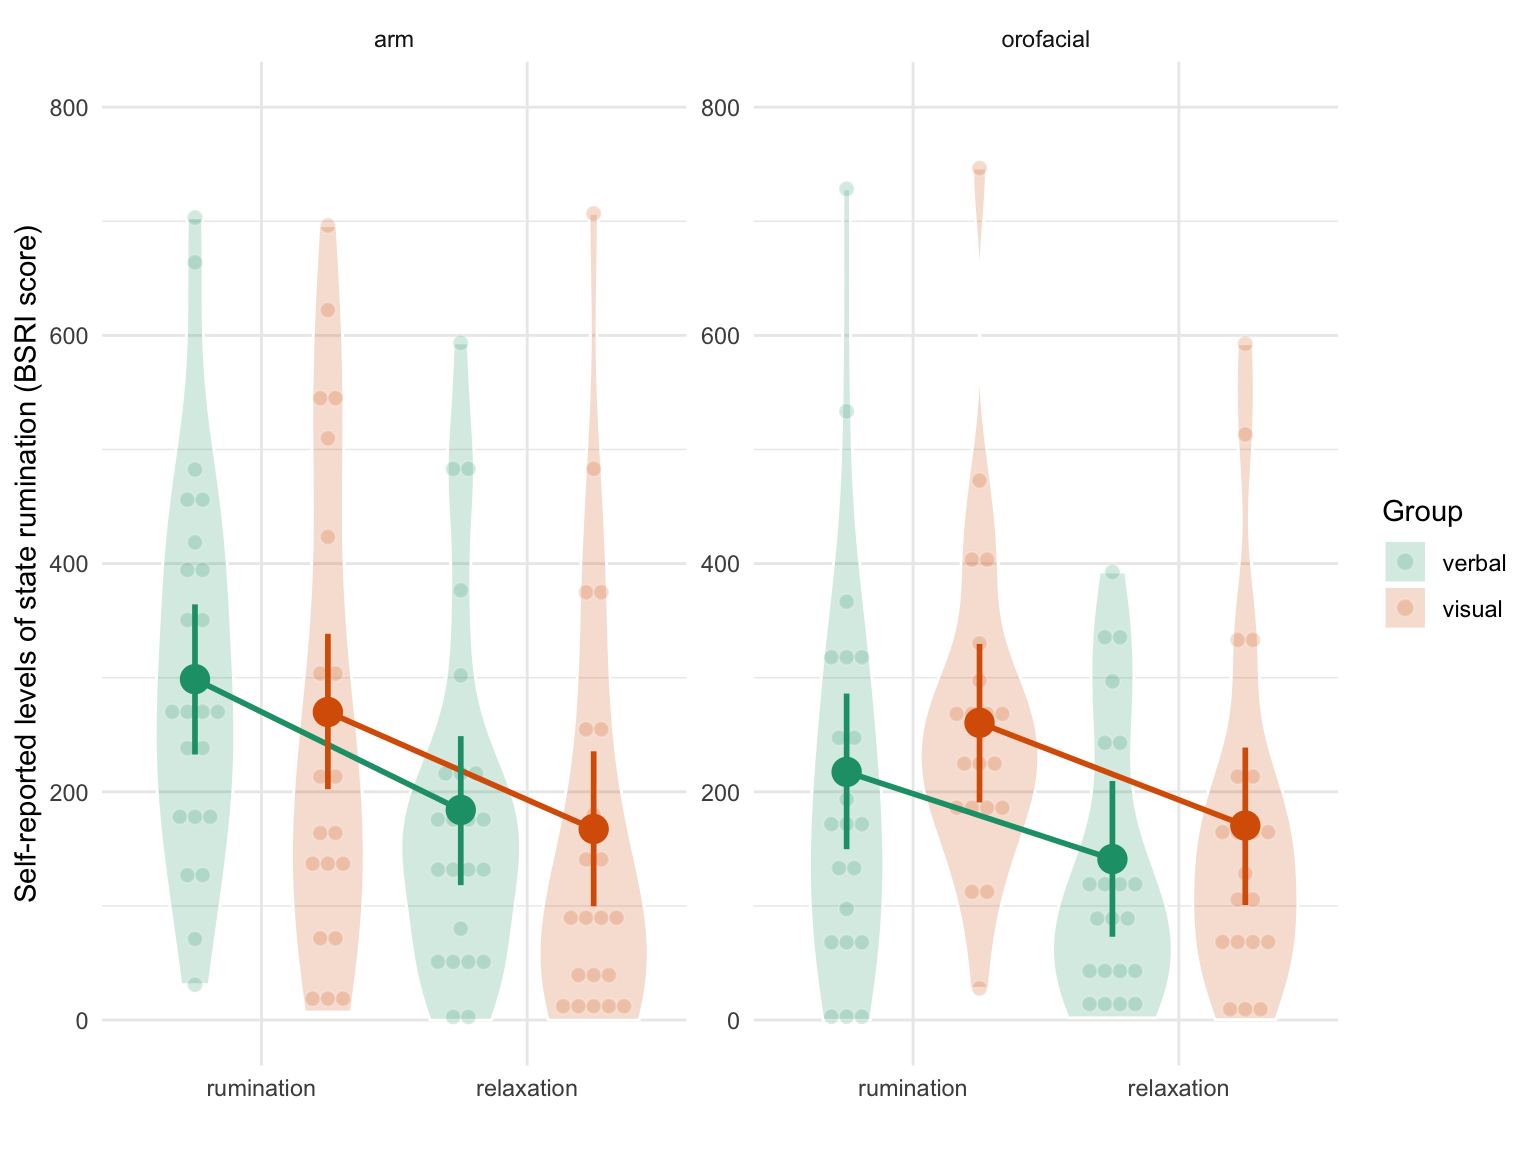
\includegraphics[width=1\linewidth]{04-chap4_files/figure-latex/plotrelaxbsri-1} 

}

\caption{Self-reported levels of state rumination (BSRI score) by condition. The left panel depicts results in the orofacial relaxation group while the right panel depicts results in the arm relaxation group. Verbal ruminators are represented in green whereas non-verbal ruminators are represented in orange. Individual observations (each participant) are represented by the smaller coloured dots whereas estimated means and 95\% CrI are represented by the bigger surimposed coloured circles and vertical error bars.}\label{fig:plotrelaxbsri}
\end{figure}

The three way interaction term (the last line of Table \ref{tab:outputbmod5}) indicates that the interaction between condition (time) and the type of relaxation was slightly different according to the type of induction type (\(\beta\) = 25.447, 95\% CrI {[}-73.748, 118.19{]}, BF\textsubscript{01} = 1.846). However, the large uncertainty associated with this three-way interaction effect (as expressed by the SE and the width of the credible interval) prevents any strong conclusion. Moreover, the sign of the BF supports the null hypothesis (although weakly in magnitude).

To sum up, we did not find evidence for an interaction effect between the type of induction (verbal vs.~non verbal) and the type of relaxation (orofacial versus arm) on the self-reported levels of state rumination. We turn now to a general summary and discussion of the overall results.

\hypertarget{discussion-1}{%
\section{Discussion}\label{discussion-1}}

With this study we aimed to replicate and extend previous findings showing that induced rumination was associated with increased facial muscular activity as compared to rest (Nalborczyk et al., \protect\hyperlink{ref-nalborczyk_orofacial_2017}{2017}). More precisely, we tried to disentangle the facial electromyographic correlates of induced rumination that were related to either i) rumination as a kind of inner speech or ii) rumination as a state of pondering on negative affects. To this end, we compared two types of rumination induction. The first one was designed to specifically induce rumination in a verbal modality, whereas the second one was designed to induce rumination in a visual imagery modality. Following the \emph{motor simulation view} of inner speech production, we hypothesised that the verbal rumination induction should result in higher activity in the speech-related muscles than the non-verbal rumination induction. At the same time, forehead muscular activity should vary consistently (i.e., should not differ) across conditions, as both conditions were expected to induce similar levels of negative affects. Following the \emph{motor simulation view} as well as previous observations (Nalborczyk et al., \protect\hyperlink{ref-nalborczyk_orofacial_2017}{2017}), we also hypothesised that a relaxation focused on the orofacial area should be more efficient in reducing rumination (when experienced in a verbal modality) than a relaxation focused on a non-orofacial area (i.e., the arm).

To examine these hypotheses, it was crucial to first show that i) the rumination induction was successful in inducing rumination and ii) that the two types of rumination induction were effectively inducing different types of rumination (i.e., verbal vs.~non-verbal rumination). Although our results show that the rumination induction was successful in inducing rumination (as expressed by the increase in self-reported state rumination), it failed to induce rumination in different modalities. That is, there was no difference in self-reported levels of verbal vs.~non verbal thoughts, and no substantial difference in the facial EMG correlates across conditions. Moreover, even when defining groups of verbal vs.~non-verbal ruminators a posteriori (i.e., based on the self-reports), these two groups were not discriminable by their facial EMG recordings. In addition, self-reported levels of state rumination were only (positively) related to the EMG amplitude of the forehead muscle (FRO), but were not related to the activity of the other facial muscles. In the second part of the experiment, comparing the two types of relaxation (either focused on the orofacial area or on the arm) revealed no difference in terms of their impact on state rumination, whatever the type of rumination induction participants went through. We discuss each of these results in the following sections.

\hypertarget{inducing-rumination-in-different-modalities}{%
\subsection{Inducing rumination in different modalities}\label{inducing-rumination-in-different-modalities}}

Based on the self-reports of verbal and visual thoughts assessed at the end of the rumination period (see Table \ref{tab:verbalvisual}), we observed that the verbal rumination induction resulted in slightly higher levels of verbal thoughts than the non-verbal rumination induction. However, both types of induction resulted in similar levels of visual mental images. These results are consistent with those of Amit et al. (\protect\hyperlink{ref-amit_asymmetrical_2017}{2017}), showing an asymmetry between inner speech and visual imagery. More precisely, they observed that inner speech production (covertly generating a sentence) was systematically accompanied by visual images. However, producing visual images was less likely to be accompanied by inner speech. Therefore, we might speculate that although it seems possible to induce verbal rumination without inducing visual rumination (and therefore to manipulate levels of verbal rumination while keeping constant levels of visual rumination), it might not be possible to induce visual rumination without inducing verbal rumination.

However, the fact that we did not find modality-specific electromyographic correlates of rumination when contrasting a posteriori groups of participants still poses a challenge to the \emph{motor simulation view}. In a recent attempt to bridge response styles theories of trait rumination (Nolen-Hoeksema, \protect\hyperlink{ref-nolen-hoeksema_responses_1991}{1991}) and control theory accounts of state rumination (Martin \& Tesser, \protect\hyperlink{ref-Martin}{1996}), rumination has been defined as a mental habit (Watkins \& Nolen-Hoeksema, \protect\hyperlink{ref-watkins_habit-goal_2014}{2014}). In this framework, self-focused repetitive thoughts (such as rumination) are triggered by goal discrepancies (i.e., discrepancies between an initial goal and the current state) and can become habitual behavioural responses to certain contextual cues. More precisely, rumination can become habitual through a process of \enquote{automatic association between the behavioral response (i.e., repetitive thinking) and any context that occurs repeatedly with performance of the behavior (e.g., physical location, mood), and in which the repetitive thought is contingent on the stimulus context} (Watkins \& Nolen-Hoeksema, \protect\hyperlink{ref-watkins_habit-goal_2014}{2014}).

Interestingly, habitual behaviours are more automatic that non-habitual behaviours, are less conscious content and are often less controllable. In other words, frequent ruminators do not willingly engage in ruminative thinking. Instead, rumination might be triggered by contextual cues such as a negative mood, without the explicit evocation of a goal (or discrepancy toward this goal). According to a recent neurocognitive model of inner speech production (Lœvenbruck et al., \protect\hyperlink{ref-loevenbruck_cognitive_2018}{2018}), inner speech is considered as an action on its own (as overt speech is), except that multimodal sensory consequences of speech are simulated. This model also suggests that different forms of inner speech might involve the speech motor system to a different extent (Lœvenbruck, \protect\hyperlink{ref-loevenbruck_what_2018}{2018}). More precisely, highly intentional forms of inner speech (e.g., subvocally rehearsing a phone number) are hypothesised to recruit the speech apparatus to a greater extent than more evasive and less intentional forms of inner speech. Accordingly, we speculate that rumination might be considered as a spontaneous (in opposition to deliberate) form of inner speech that does not require a full specification of articulatory features.

As such, we might actually not expect to observe peripheral muscular activity during rumination. If this hypothesis is correct, we need to explain the increased EMG amplitude recorded over the OOI after the rumination induction that was observed in this experiment but also in Nalborczyk et al. (\protect\hyperlink{ref-nalborczyk_orofacial_2017}{2017}). Given that only the activity of the \emph{frontalis} (FRO) was related to self-reported levels of state rumination (although this relation was rather weak), it is difficult to assume that the activity of the other muscles was related to rumination per se. In addition, the lack of a proper control condition (e.g., a distraction condition) prevents any causal conclusion to be drawn. Therefore, the most straightforward explanation may be that the increase in EMG amplitude recorded over the OOI might only appear in contrast to the relaxation state induced at baseline.

Finally, another explanation for the absence of modality-specific EMG correlates might come from studies using surface EMG to investigate inner speech production. As summarised in the previous section, our results do not support theoretical predictions of the \emph{motor simulation view}, according to which it should be possible to discriminate the content of inner speech (and rumination) based on peripheral muscular activation. Nevertheless, the outcome of the present study is consistent with the results reported by Meltzner et al. (\protect\hyperlink{ref-meltzner_speech_2008}{2008}). These authors were able to obtain high classification accuracies during both overt and mouthed speech but not during covert speech (despite the fact that they used eleven sensors on the neck and the lower face).

However, the results of Meltzner et al. (\protect\hyperlink{ref-meltzner_speech_2008}{2008}) (and ours) stand in sharp contrast with classical results about the electromyographic correlates of inner speech production (e.g., McGuigan \& Dollins, \protect\hyperlink{ref-mcguigan_patterns_1989}{1989}; McGuigan \& Winstead, \protect\hyperlink{ref-mcguigan_discriminative_1974}{1974}; Sokolov, \protect\hyperlink{ref-sokolov_inner_1972}{1972}) as well as more recent developments. For instance, Kapur et al. (\protect\hyperlink{ref-kapur_alterego_2018}{2018}) developed a wearable device composed of seven surface EMG sensors that can attain a 92\% median classification accuracy in discriminating internally vocalised digits. However, these different results be explained by differences in the research methodology employed by these different teams (see discussion in Nalborczyk et al., \emph{in preparation}). Indeed, the between-subject nature of the designs investigating the effects of induced rumination might hamper the possibility of highlighting modality-specific EMG correlates of induced rumination. Because (surface) electromyography is only a noisy indicator of inner speech production, decoding the content of inner speech based on such signals require multiple measurements per individual, and possibly participant-specific recording characteristics. Therefore, the lack of modality-specific EMG correlates might also be explained by a lack of sensitivity of the design we describe in the current article.

We think this possibility might be examined by looking at the results obtained in the second part of the experiment. If the absence of modality-specific EMG correlates is only due to a lack of sensitivity, state rumination should still be more disrupted by an orofacial relaxation than by a non-orofacial relaxation.

\hypertarget{modality-specific-and-effector-specific-relaxation-effects}{%
\subsection{Modality-specific and effector-specific relaxation effects}\label{modality-specific-and-effector-specific-relaxation-effects}}

Contrary to our predictions, we did not observe the interaction effect between the type of rumination induction (verbal vs.~non-verbal) and the type of relaxation (orofacial relaxation vs.~arm relaxation). This null result also persisted when considering the interaction between the a posteriori cluster and the type of relaxation (see \protect\hyperlink{suppCh4}{supplementary materials}). Moreover, BF-based hypothesis testing revealed no evidence for a difference between the two types of relaxation\footnote{Neither did it reveal evidence for a difference, as the BF was close to 1. A Bayes factor around 1 means that the observed data is similarly likely to appear under both the hypothesis of an effect being different from zero and the hypothesis of a null effect. Moreover, it should be noted that BFs are extremely dependent on prior assumptions. As such, the obtained BFs might vary substantially by varying the prior assumptions of the fitted models.} (cf.~Table \ref{tab:outputbmod5} and Figure \ref{fig:plotrelaxbsri}). However, looking in more details into the estimations from this model reveals that the arm relaxation was estimated to be more efficient than the orofacial relaxation in reducing self-reported levels of state rumination (BSRI scores). More precisely, the difference between the two types of relaxations was estimated to be of around 25 points on the scale of the BSRI sum score, although the large uncertainty associated with this estimation prevents any strong conclusion.

Interestingly, these results are contradicting those of Nalborczyk et al. (\protect\hyperlink{ref-nalborczyk_orofacial_2017}{2017}), who observed a stronger decrease in self-reported state rumination following the orofacial relaxation than the arm relaxation. However, it should be noted that both the results of Nalborczyk et al. (\protect\hyperlink{ref-nalborczyk_orofacial_2017}{2017}) and the results reported in the current article are based on comparisons involving relatively low sample sizes (two groups of around 20 participants and two groups of around 40 participants, respectively). As such, these results should be considered at most as suggestive.

Nevertheless, the high similarity between these two studies warrants a meta-analytical way of thinking about their results. In other words, given that both studies used a similar rumination induction and the same relaxation recordings, we can compute an average effect size across these two studies to get a more accurate estimate of the population effect size. The effect size (pooled Cohen's d) for the difference between the two types of relaxation was of \(\delta\) = -0.498 (95\% CI {[}-1.095, 0.098{]}) in Nalborczyk et al. (\protect\hyperlink{ref-nalborczyk_orofacial_2017}{2017}) and of \(\delta\) = 0.217 (95\% CI {[}-0.216, 0.65{]}) in the current article. Because the current study has a larger sample size, the uncertainty (the width of the CI) about the value of the Cohen's d is smaller. Therefore, weighting both estimates by their respective standard error reveals an average effect size that is very close to zero (\(\delta\) = -0.052).

To sum up, we did not observe a stronger effect of the orofacial relaxation (when compared to the non-orofacial relaxation) and we did not observe the hypothesised interaction effect between the type of rumination induction and the type of relaxation. Moreover, we also did not observe an interaction between the type of rumination induction and the clusters defined a posteriori (see \protect\hyperlink{suppCh4}{supplementary materials}). These results taken together corroborate the hypothesis formulated previously, according to which rumination --as a mental habit (Watkins \& Nolen-Hoeksema, \protect\hyperlink{ref-watkins_habit-goal_2014}{2014})-- could be considered as a strongly internalised form of inner speech. As such, ruminative thinking would not \emph{require} the involvement of the speech motor system. Therefore, rumination is not expected to be disrupted by motor interferences such as relaxation or articulatory suppression (Nalborczyk et al., \emph{submitted}).

\hypertarget{conclusions}{%
\subsection{Conclusions}\label{conclusions}}

We aimed to evaluate whether rumination is better described as a form of inner speech that requires the motor simulation of speech production, or as a rather abstract and articulatory impoverished form of inner speech. In the first case, verbal rumination should be accompanied by an activation of the speech muscles and should be disrupted by motor interference directed at the speech muscles. To examine these hypotheses, we extended a previous study (Nalborczyk et al., \protect\hyperlink{ref-nalborczyk_orofacial_2017}{2017}) and compared two types of rumination induction designed to induce either verbal or non-verbal (visual) rumination.

In the first part of the experiment, we replicated the findings of Nalborczyk et al. (\protect\hyperlink{ref-nalborczyk_orofacial_2017}{2017}) by showing that both the activity of the forehead (FRO) and the activity of the lip (OOI) was higher than baseline after a rumination induction (averaging across the two types of rumination induction). However, we failed to find distinct EMG correlates when comparing the two types of rumination induction or when comparing two (a posteriori defined) groups of verbal vs.~non-verbal ruminators. Moreover, only the activity of the forehead was related to self-reported state rumination. In the second part of the experiment, we did not observe the hypothesised interaction effect between the type of induction and the type of relaxation. More precisely, following the \emph{motor simulation view} of inner speech production, we expected to observe a stronger decrease in self-reported state rumination following an orofacial relaxation than a non-orofacial relaxation, when rumination was expressed in a verbal modality (as compared to a non-verbal modality). This prediction was not supported by the data. Taken together, these results suggest that verbal rumination is a somehow impoverished form of inner speech that is not fully specified at an articulatory level.

We speculated that this observation might be explained by the degree of automaticity that usually accompanies rumination. Following the mental habit view of rumination (Watkins \& Nolen-Hoeksema, \protect\hyperlink{ref-watkins_habit-goal_2014}{2014}), rumination can be considered as an habitual mode of response to contextual cues (e.g., negative mood). As such, it can be considered as a non-intentional (or weakly intentional) form of inner speech. Thus, the absence of modality-specific correlates of verbal rumination is congruent with the observation that inner speech is more strongly accompanied by peripheral muscular activation when expressed intentionally or under adverse conditions (e.g., Sokolov, \protect\hyperlink{ref-sokolov_inner_1972}{1972}).

Some limitations are worth keeping in mind when interpreting these results. First, the current sample only consisted of female participants. Whereas it permitted to maximise the probability of effectively inducing rumination, it also limits the generalisability of these findings. Second, although the rumination induction resulted in slightly different levels of self-reported levels of verbal thoughts, this difference was weak. Instead of \emph{inducing} rumination in different modalities, a more fruitful strategy to compare the consequences of verbal vs.~non-verbal rumination might be to induce rumination in the \enquote{preferred} modality of the participant. We might recruit participants with a propensity to ruminate preferentially in one of those modalities and present them with a classical rumination induction procedure. This would arguably increase the contrast between the two type of inductions and the probability of observing modality-specific EMG correlates, if any.

Nevertheless, these results provide relevant information for both the study of repetitive negative thinking (including rumination) and the study of inner speech. On the first hand, the strong internalisation of verbal rumination speaks in favour of the conception of rumination as a mental habit (Watkins \& Nolen-Hoeksema, \protect\hyperlink{ref-watkins_habit-goal_2014}{2014}). On the other hand, the modulation of the involvement of the speech motor system during inner speech by its degree of automaticity is congruent with previous observations. However, these results still need to be explained by and incorporated into integrative neurocognitive models of inner speech production.

\hypertarget{suppCh4}{%
\section{Supplementary materials}\label{suppCh4}}

Pre-registered protocol, open data, supplementary analyses as well as reproducible code and figures are available at \url{https://osf.io/c9pag/}.

Many packages have been used for the writing of this paper, among which the \texttt{BEST}, \texttt{patchwork} and \texttt{ggplot2} packages for plotting (Kruschke \& Meredith, \protect\hyperlink{ref-R-BEST}{2018}; Pedersen, \protect\hyperlink{ref-R-patchwork}{2017}; Wickham et al., \protect\hyperlink{ref-R-ggplot2}{2018}), the \texttt{tidybayes} and \texttt{sjstats} packages for data analysis (Kay, \protect\hyperlink{ref-R-tidybayes}{2018}; Lüdecke, \protect\hyperlink{ref-R-sjstats}{2018}), as well as the \texttt{glue} and \texttt{tidyverse} packages for code writing and formatting (Hester, \protect\hyperlink{ref-R-glue}{2017}; Wickham, \protect\hyperlink{ref-R-tidyverse}{2017}).

\hypertarget{acknowledgements-1}{%
\section{Acknowledgements}\label{acknowledgements-1}}

This project was funded by the ANR project INNERSPEECH (grant number ANR-13-BSH2-0003-01). LN was funded by a PhD fellowship from Univ. Grenoble Alpes. We thank Nathalie Vallet for recording the relaxation sessions.

\newpage

\begin{vplace}[1]

\begin{summary}{Summary of Chapter\getcurrentref{chapter}}

In this chapter, we sought to examine the differences (if any) between different forms of induced rumination, that should theoretically involve the speech motor system to a different extent. We compared the EMG orofacial correlates of either verbal rumination or non-verbal (visual) rumination. Unfortunately, self-reports of the modal content of the ruminative thoughts showed that our induction did not succeed in inducing rumination in different modalities. However, even when exploring the (a posteriori) relation between the modality of the ruminative thoughts and the facial EMG correlates, we failed to find the predicted relation. Put simply, verbal rumination was not associated with more activity in the speech muscles than non-verbal rumination. Moreover, comparing two types of relaxation revealed that, in contrast to previous results (cf. Chapter 3), the arm relaxation was slightly more efficient than the orofacial relaxation in reducing state rumination. Averaging the relaxation results from these two first studies revealed that both relaxation types have a similar effect on state rumination. These results therefore suggest that verbal rumination is not specifically accompanied with peripheral muscular activity in the speech muscles. However, it is unclear whether this result is due to a poor sensitivity of the surface EMG measurements or to the fact that rumination is a form of inner speech that does not involve the speech motor system. In the next chapter, we seek to resolve that ambiguity by examining the reliability of our EMG measurements to detect peripheral muscular activity during inner speech production.

\end{summary}

\end{vplace}

\hypertarget{chap5}{%
\chapter{Muscle-specific electromyographic correlates of inner speech production}\label{chap5}}

\initial{D}espite a long history of scrutiny in experimental psychology, it is still controversial whether inner speech (covert speech) production is accompanied by peripheral muscular activity in the speech muscles. We address this question by briefly reviewing previous findings related to the phenomenon of inner speech and to the broader phenomenon of motor imagery. We then present the results of a preregistered experiment looking at the electromyographic correlates of both overt speech and inner speech production of two classes of nonwords. An automatic classification approach was undertaken to discriminate these signals according to the class of nonword to be uttered. Although this approach lead to reasonable accuracy rates during overt speech production, it failed to discriminate inner speech content based on surface electromyography signals. We discuss these results in relation to other recent results and suggest alternative ways to test the engagement of the speech motor system during inner speech production.\footnote{This experimental chapter is a submitted manuscript reformatted for the need of this thesis. Pre-registered protocol, preprint, data, as well as reproducible code and figures are available at: \url{https://osf.io/czer4/}.}

\hypertarget{introduction-2}{%
\section{Introduction}\label{introduction-2}}

As you read these words, you are likely experiencing the presence of a familiar speechlike companion. This inner voice usually accompanies daily activities such as reading or writing and is estimated to be present at least one quarter of our awaken life (Heavey \& Hurlburt, \protect\hyperlink{ref-heavey_phenomena_2008}{2008}). By deliberately paying attention to this voice, one can examine its phenomenological properties such as identity (whose voice is it ?) or other high-level characteristics (e.g., is it gendered ?). It is also possible to examine lower-level features like the tone of the voice, its pitch or its tempo.

This first set of basic observations leads to some important insights about the nature of inner speech. First, if we can think about inner speech, then it should be something different from thinking itself. Second, the simple fact that we can make sensory judgements about our inner voice tautologically reveals that inner speech is accompanied by sensory percepts (e.g., speech sounds, kinaesthetic feelings). This leads to other fundamental questions: where do these percepts come from ? Why do they look like the one we experience when we \emph{actually} (overtly) speak ?

Two main classes of explanatory models have been suggested to answer these questions. A first class of theories is described under the umbrella term of \emph{motor simulation view}. These theories broadly suggest that inner speech can be conceived as a kind of action on its own (Simon R Jones \& Fernyhough, \protect\hyperlink{ref-Jones2007}{2007}; Martínez-Manrique \& Vicente, \protect\hyperlink{ref-Martinez-Manrique2015}{2015}) in the same way as overt speech is, except that speech percepts (e.g., speech sounds) are simulated. Most theories under this view share the postulate that the speech motor system is involved (to some extent) during inner speech production. In contrast, a second class of theories, that we describe as the \emph{abstraction view}, suggest that inner speech results from the activation of abstract linguistic representations (e.g., Oppenheim \& Dell, \protect\hyperlink{ref-oppenheim_inner_2008}{2008}) that do not involve lower-level features (e.g., articulatory representations).

Previous research have demonstrated that it is possible to record muscle-specific electromyographic correlates of inner speech (e.g., McGuigan \& Dollins, \protect\hyperlink{ref-mcguigan_patterns_1989}{1989}; McGuigan \& Winstead, \protect\hyperlink{ref-mcguigan_discriminative_1974}{1974}). However, these studies mostly focused on small samples of children and sometimes used invasive intramuscular electromyography. In contrast, more recent research using surface electromyography in adult samples lead to mixed results (e.g., Meltzner et al., \protect\hyperlink{ref-meltzner_speech_2008}{2008}). Building upon previous work, we describe an experimental set-up using surface electromyography with the aim of testing the involvement of the speech motor system during inner speech production.

\hypertarget{inner-speech-as-motor-imagery-of-speech}{%
\section{Inner speech as motor imagery of speech}\label{inner-speech-as-motor-imagery-of-speech}}

Speech production is an incredibly complex motor action, involving the fine-grained coordination of more than 100 muscles in the upper part of the body (Simonyan \& Horwitz, \protect\hyperlink{ref-simonyan_laryngeal_2011}{2011}). In adult humans, its covert counterpart (i.e., \emph{inner speech} or \emph{verbal imagery}) has developed to support a myriad of different functions. In the same way as visual imagery permits to mentally examine visual scenes, \emph{verbal imagery} can be used as an internal tool, allowing --amongst other things-- to rehearse or to prepare past and future conversations (for review, see Alderson-Day \& Fernyhough, \protect\hyperlink{ref-alderson-day_inner_2015}{2015}; Perrone-Bertolotti et al., \protect\hyperlink{ref-Perrone-Bertolotti2014}{2014}). Because speech production results from sequences of motor commands which are assembled to reach a given goal, it belongs to the broader category of motor actions (Jeannerod, \protect\hyperlink{ref-jeannerod_motor_2006}{2006}). Therefore, a parallel can be drawn between verbal imagery and other forms of motor imagery (e.g., imagined walking or imagined writing). Accordingly, studies on the nature of inner speech might benefit from insights gained from the study of motor imagery and the field of motor cognition (e.g., Haggard, \protect\hyperlink{ref-haggard_conscious_2005}{2005}; Jeannerod, \protect\hyperlink{ref-jeannerod_motor_2006}{2006}).

Motor imagery can be defined as the mental process by which one rehearses a given action, without engaging in the physical movements involved in this particular action. One of the most influential theoretical explanation of this broad phenomenon is the \emph{motor simulation theory} (MST; Jeannerod, \protect\hyperlink{ref-jeannerod_representing_1994}{1994}, \protect\hyperlink{ref-jeannerod_neural_2001}{2001}, \protect\hyperlink{ref-jeannerod_motor_2006}{2006}). In this framework, the concept of simulation refers to the \enquote{offline rehearsal of neural networks involved in specific operations such as perceiving or acting} (Jeannerod, \protect\hyperlink{ref-jeannerod_motor_2006}{2006}, p. 29) and motor imagery is conceptualised as a simulation of the covert stage of the same executed action (O'Shea \& Moran, \protect\hyperlink{ref-oshea_does_2017}{2017}). The MST shares some similarities with the theories of embodied and grounded cognition (Barsalou, \protect\hyperlink{ref-Barsalou2008}{2008}) in that both account for the phenomenon of motor imagery by appealing to a simulation mechanism. However, the concept of simulation in grounded theories is assumed to operate in order to achieve a particular abstract knowledge (O'Shea \& Moran, \protect\hyperlink{ref-oshea_does_2017}{2017}), which is not the concern of the MST. In other words, we should make a distinction between \emph{embodiment of content}, which concerns the conceptual content of language, and \emph{embodiment of form}, which concerns \enquote{the vehicle of thought}, that is, proper speech production (Pickering \& Garrod, \protect\hyperlink{ref-pickering_integrated_2013}{2013}).

A second class of explanatory models of motor imagery are concerned with the phenomenon of \emph{emulation} and with \emph{internal models} (see Gentsch, Weber, Synofzik, Vosgerau, \& Schütz-Bosbach, \protect\hyperlink{ref-gentsch_towards_2016}{2016}, for a review of the similarities and dissimilarities between simulation and emulation models). Internal model theories share the postulate that action control uses internal models, that is, systems that simulate the behaviour of the motor apparatus (Jordan \& Rumelhart, \protect\hyperlink{ref-jordan_forward_1992}{1992}; Kawato et al., \protect\hyperlink{ref-kawato_hierarchical_1987}{1987}). The function of internal models is to estimate and anticipate the outcome of a motor command. Among the internal model theories, motor control models based on robotic principles (e.g., Kawato, \protect\hyperlink{ref-kawato_internal_1999}{1999}; Wolpert et al., \protect\hyperlink{ref-wolpert_internal_1995}{1995}) assume two kinds of internal models (that are supposed to be coupled and regulated): a forward model (or simulator) that predicts the sensory consequences of motor commands from efference copies of the issued motor commands, and an inverse model (or controller) that calculates the feedforward motor commands from the desired sensory states (Gentsch et al., \protect\hyperlink{ref-gentsch_towards_2016}{2016}; Lœvenbruck et al., \protect\hyperlink{ref-loevenbruck_cognitive_2018}{2018}).

Emulation theories (e.g., Grush, \protect\hyperlink{ref-grush_emulation_2004}{2004}; Moulton \& Kosslyn, \protect\hyperlink{ref-moulton_imagining_2009}{2009}) borrow from both simulation theories and internal model theories to posit a specific kind of simulation. In the emulation model proposed by Grush (\protect\hyperlink{ref-grush_emulation_2004}{2004}), the \emph{emulator} is a device that implements the same input-output function as the body (i.e., the musculoskeletal system and relevant proprioceptive/kinaesthetic systems)\footnote{In Grush's terminology, \emph{emulator} is used as a synonym for \emph{forward model} (see Grush, \protect\hyperlink{ref-grush_emulation_2004}{2004}, pp. 378--379).}. When the emulator receives a copy of the control signal (which is also sent to the body), it produces an output signal (the emulator feedback), identical or similar to the feedback signal produced by the body, yielding mock sensory percepts (e.g., visual, auditory, kinaesthetic) during motor imagery.

By building upon models of speech motor control (e.g., Houde \& Nagarajan, \protect\hyperlink{ref-houde_speech_2011}{2011}; Wolpert et al., \protect\hyperlink{ref-wolpert_internal_1995}{1995}), a recent model describes wilful (voluntary) expanded inner speech as \enquote{multi-modal acts with multi-sensory percepts stemming from coarse multi-sensory goals} (Lœvenbruck et al., \protect\hyperlink{ref-loevenbruck_cognitive_2018}{2018}). In other words, in this model the auditory and kinaesthetic sensations perceived during inner speech are assumed to be the predicted sensory consequences of speech motor acts, emulated by internal forward models that use the efference copies issued from an inverse model (this proposal shares similarities with the emulation model of motor imagery, Grush, \protect\hyperlink{ref-grush_emulation_2004}{2004}). It should be noted that both simulation, emulation, and motor control frameworks can be grouped under the \emph{motor simulation view} and altogether predict that the motor system should be involved to some extent during motor imagery, and by extension, during inner speech production. We turn now to a discussion of findings related to peripheral muscular activity during motor imagery and inner speech.

\hypertarget{electromyographic-correlates-of-covert-actions}{%
\section{Electromyographic correlates of covert actions}\label{electromyographic-correlates-of-covert-actions}}

Across both simulationist and emulationist frameworks, motor imagery has consistently been defined as the mental rehearsal of a motor action without any overt movement. One consequence of this claim is that, in order to prevent execution, the neural commands for muscular contractions should be blocked at some level of the motor system by active inhibitory mechanisms (for a review, see Guillot et al., \protect\hyperlink{ref-guillot_imagining_2012}{2012}\protect\hyperlink{ref-guillot_imagining_2012}{a}). Despite these inhibitory mechanisms, there is now abundant evidence for peripheral muscular activation during motor imagery (for a review, see Guillot \& Collet, \protect\hyperlink{ref-guillot_contribution_2005}{2005}; Guillot et al., \protect\hyperlink{ref-guillot_imagining_2012}{2012}\protect\hyperlink{ref-guillot_imagining_2012}{a}, \protect\hyperlink{ref-guillot_electromyographic_2010}{2010}). As suggested by Jeannerod (\protect\hyperlink{ref-jeannerod_representing_1994}{1994}), the incomplete inhibition of the motor commands would provide a valid explanation to account for the peripheral muscular activity observed during motor imagery. This idea has been corroborated by studies of changes in the excitability of the motor pathways during motor imagery tasks (for a review, see Stinear, \protect\hyperlink{ref-stinear_corticospinal_2010}{2010}). For instance, Bonnet et al. (\protect\hyperlink{ref-bonnet_mental_1997}{1997}) measured spinal reflexes while participants were instructed to either press a pedal with the foot or to simulate the same action mentally. They observed that both H-reflexes and T-reflexes increased during motor imagery, and that these increases correlated with the force of the simulated pressure. Using transcranial magnetic stimulation and motor evoked potentials (MEPs), several investigators observed muscle-specific increases of MEPs during various motor imagery tasks, whereas no such increase could be observed in antagonist muscles (e.g., Fadiga et al., \protect\hyperlink{ref-fadiga_corticospinal_1999}{1999}; Rossini, \protect\hyperlink{ref-rossini_corticospinal_1999}{1999})\footnote{As a side note, we should remark that these findings are consistent with both the simulation and the emulation views on motor imagery.}.

When considered as a form of motor imagery, inner speech production is also expected to be accompanied with peripheral muscular activity in the speech muscles. This idea is supported by many studies showing peripheral muscular activation during inner speech production (e.g., Livesay et al., \protect\hyperlink{ref-livesay_covert_1996}{1996}; Locke, \protect\hyperlink{ref-locke_subvocal_1970-1}{1970}; Locke \& Fehr, \protect\hyperlink{ref-locke_subvocal_1970}{1970}; McGuigan \& Dollins, \protect\hyperlink{ref-mcguigan_patterns_1989}{1989}; McGuigan \& Winstead, \protect\hyperlink{ref-mcguigan_discriminative_1974}{1974}; Sokolov, \protect\hyperlink{ref-sokolov_inner_1972}{1972}), during auditory verbal hallucinations in patients with schizophrenia (Rapin et al., \protect\hyperlink{ref-rapin_emg_2013}{2013}\protect\hyperlink{ref-rapin_emg_2013}{a}), or during induced mental rumination (Nalborczyk et al., \protect\hyperlink{ref-nalborczyk_orofacial_2017}{2017}). Some authors also recently demonstrated that it is possible to discriminate inner speech content based on surface electromyography signals with a median 92\% accuracy (Kapur et al., \protect\hyperlink{ref-kapur_alterego_2018}{2018}). However, other teams failed to obtain such results (e.g., Meltzner et al., \protect\hyperlink{ref-meltzner_speech_2008}{2008}).

Many of these EMG studies concluded on the involvement of the speech motor system based on a difference in EMG amplitude when contrasting a period of inner speech production with a period of rest. However, as highlighted by Garrity (\protect\hyperlink{ref-garrity_electromyography_1977}{1977}), it is usually not enough to show an increase of speech muscle activity during inner speech to conclude that this activation is related to inner speech production. Three sorts of inference can be made through electromyographic studies of inner speech production, depending on the stringency of the control procedure. The stronger sort of inference is permitted by highlighting a discriminative pattern during covert speech production, as for instance when demonstrating a dissociation between different speech muscles during the production of speech sounds of different phonemic class (e.g, contrasting labial versus non-labial words). According to Garrity (\protect\hyperlink{ref-garrity_electromyography_1977}{1977}), other (weaker) types of control procedures include i) comparing the EMG activity during covert speech production to a baseline period (without contrasting phonemic classes in covert speech utterances), or ii) comparing the activity of speech-related and non-speech related (e.g., forearm) muscle activity. Ideally, these controls can be combined by recording and contrasting speech and non-speech related muscles in different conditions (e.g., rest, covert speech, overt speech) of pronunciation of different speech sounds classes (e.g., labial versus non-labial).

Previous research carried out using the preferred procedure recommended by Garrity (\protect\hyperlink{ref-garrity_electromyography_1977}{1977}) suggest a discriminative patterns of electromyographic correlates according to the phonemic class of the words being covertly uttered (e.g., McGuigan \& Dollins, \protect\hyperlink{ref-mcguigan_patterns_1989}{1989}; McGuigan \& Winstead, \protect\hyperlink{ref-mcguigan_discriminative_1974}{1974}), which would corroborate the \emph{motor simulation view} of inner speech. However, these studies used limited sample sizes (often less than ten participants), worked mostly with children participants and used signal processing methods that are now outdated. These factors limit the generalisability of the above findings because i) low-powered experiments provide biased estimates of effects, ii) following the natural internalisation process, inner speech muscular correlates are expected to weaken with age and iii) a higher sensitivity could be attained by using modern sensors and signal processing methods.

The present study then aims to decide between the \emph{motor simulation view} and the \emph{abstraction view} of inner speech, and can be seen as a conceptual replication and extension of previous works carried out by McGuigan and collaborators (e.g., McGuigan \& Dollins, \protect\hyperlink{ref-mcguigan_patterns_1989}{1989}; McGuigan \& Winstead, \protect\hyperlink{ref-mcguigan_discriminative_1974}{1974}). We aimed to examine whether it is possible to demonstrate similar dissociations by using surface electromyography recorded over the lip (\emph{orbicularis oris inferior}) and the \emph{zygomaticus major} muscles. More precisely, if the \emph{motor simulation view} is correct, we should observe a higher average EMG amplitude recorded over the OOI during both the overt and inner production of rounded nonwords in comparison to spread nonwords. Conversely, we would expect a lower average EMG amplitude recorded over the ZYG during both the inner and overt production of rounded nonwords in comparison to spread nonwords. In addition, we would not expect to observe content-specific differences in EMG amplitude concerning the non speech-related muscles (i.e., forehead and forearm muscles).

\hypertarget{methods-2}{%
\section{Methods}\label{methods-2}}

In the \emph{Methods} and \emph{Data analysis} sections, we report how we determined our sample size, all data exclusions, all manipulations, and all measures in the study (Simmons et al., \protect\hyperlink{ref-simmons_21_2012}{2012}). A pre-registered version of our protocol can be found on OSF: \url{https://osf.io/czer4/}.

\hypertarget{participants-2}{%
\subsection{Participants}\label{participants-2}}

As previous studies of the electromyographic correlates of inner speech were mostly carried out with samples of children or young adults, used different kinds of EMG measures (surface EMG or needle EMG), and different kinds of signal processing methods, it was impractical how to determine the effect size of interest for the current study. Therefore, we used sequential testing as our sampling procedure, based on the method described in Schönbrodt \& Wagenmakers (\protect\hyperlink{ref-schonbrodt_bayes_2018}{2018}) and Schönbrodt, Wagenmakers, Zehetleitner, \& Perugini (\protect\hyperlink{ref-schonbrodt_sequential_2017}{2017}). We fixed a statistical threshold to \(BF_{10} = 10\) and \(BF_{10} = \dfrac{1}{10}\) (i.e., \(BF_{01} = 10\)), testing the difference between the inner production of labial items versus the inner production of non-labial items on the standardised EMG activity of the lower lip (\emph{orbicularis oris inferior}). In order to prevent potential experimenter and demand biases during sequential testing, the experimenter was blind to BFs computed on previous participants (Beffara, Bret, \& Nalborczyk, 2018). All statistical analyses have been automatised and a single instruction was returned to the experimenter (i.e., \enquote{keep recruiting participants} or \enquote{stop the recruitment}). We fixed the maximum sample size to 100 participants.

As a result of the above sampling procedure, a total of 26 French-speaking undergraduate students in Psychology from the Univ. Grenoble Alpes took part in this experiment, in exchange for course credits\footnote{NB: this procedure did not work optimally because we later spotted a mistake in the EMG signal processing workflow. Thus, the sequential testing stopped earlier than it should have.}. They were recruited via mailing list, online student groups, and posters. Each participant provided a written consent and the present study was approved by the local ethics committee.

\hypertarget{material-2}{%
\subsection{Material}\label{material-2}}

\hypertarget{emg-recordings}{%
\subsubsection{EMG recordings}\label{emg-recordings}}

EMG activity was recorded using TrignoTM Mini sensors (Delsys Inc.) at a sampling rate of 1926 samples/s with a band pass of 20 Hz (12 dB/ oct) to 450 Hz (24 dB/oct) and were amplified by a TrignoTM 16-channel wireless EMG system (Delsys Inc.). These sensors consist of two 5 mm long, 1 mm wide parallel bars, spaced by 10 mm, which were attached to the skin using double-sided adhesive interfaces. The skin was cleaned by scrubbing it with 70\% isopropynol alcohol. EMG signals were synchronised using the PowerLab 16/35 (ADInstrument, PL3516). Raw data from the EMG sensors were then resampled at a rate of 1 kHz and stored in digital format using Labchart 8 software (ADInstrument, MLU60/8). EMG sensors were positioned over five muscles: the \emph{corrugator supercilii} (COR), the \emph{frontalis} (FRO), the \emph{zygomaticus major} (ZYG), the \emph{orbicularis oris inferior} (OOI), and the \emph{flexor carpi radialis} (FCR). The two speech-related muscles (OOI and ZYG) were chosen to show content-specific EMG correlates, whereas the two non-speech related facial muscles (ZYG and FRO) were chosen to control for higher overall facial muscular activity. We also recorded the activity of the FCR of the non-dominant forearm to control for overall (whole body) higher muscular activity.

We recorded the activity of control and emotion-linked muscles (i.e., COR and FRO) that were positioned on the non-dominant side of the face (i.e., the left side for right-handed participants), while sensors recording the activity of the speech muscles (i.e., ZYG and OOI) were positioned on the dominant side of the face. As reviewed in Everdell et al. (\protect\hyperlink{ref-everdell_gaze_2007}{2007}), the dominant side of the face displays larger movements than the left side during speech production, whereas the non-dominant side is more emotionally expressive.

The experiment was video-monitored using a Sony HDR-CX240E video camera to track any visible facial movements. A microphone was placed 20--30 cm away from the participant's lips to record any faint vocal production during rumination. Stimuli were displayed using the OpenSesame software (Mathôt et al., \protect\hyperlink{ref-mathot_opensesame_2012}{2012}) on a 19-inch colour monitor.

\hypertarget{nonwords}{%
\subsubsection{Linguistic material}\label{nonwords}}

We selected ten rounded and ten spread bi-syllabic nonwords (see Table \ref{tab:words}). Each class of nonwords was specifically designed to either induce a greater activation of the lip muscle (rounded items) or a greater activation of the zygomaticus muscle (spread items). Rounded items consisted in the repetition of a syllable containing a bilabial consonant followed by a rounded vowel, whereas spread items consisted in the repetition of a syllable containing a lingual consonant followed by a spread vowel.

\begin{table}[H]
\begin{center}
\begin{threeparttable}
\caption{\label{tab:words}List of bisyllabic nonwords used in the test session.}
\begin{tabular}{cc}
\toprule
rounded items & \multicolumn{1}{c}{spread items}\\
\midrule
/mumu/ & /gigi/\\
/pupu/ & /sese/\\
/fofo/ & /lele/\\
/mymy/ & /sisi\\
/pypy/ & /didi/\\
/byby/ & /nini/\\
/vøvø/ & /ʒiʒi/*\\
/pøpø/ & /lili/\\
/bøbø/ & /ʁiʁi/\\
/mɔ̃mɔ̃/ & /gege/\\
\bottomrule
\addlinespace
\end{tabular}
\begin{tablenotes}[para]
\textit{Note.} *Because the production of /ʒiʒi/ requires a protrusion of the lips, this item theoretically slightly deviates from other items of this class.
\end{tablenotes}
\end{threeparttable}
\end{center}
\end{table}

\hypertarget{procedure-2}{%
\subsection{Procedure}\label{procedure-2}}

Participants were seated in front of a computer screen while audio stimuli (when applicable) were presented through speakers on both sides of the screen. A video camera was positioned on one side of the screen to monitor facial movements. After positioning of the EMG sensors, each participant underwent a relaxation session aiming to minimise pre-existing inter-individual variability on facial muscle contraction (approximate duration was 330s). This relaxation session was recorded by a trained professional sophrology therapist. Baseline EMG measurements were performed during the last minute of this relaxation period, resulting in 60s of EMG signals at baseline. Subsequently, participants went through a training session, during which they could get familiar with the main task. They trained with 8 stimuli in total (4 rounded nonwords and 4 spread nonwords)\footnote{The training list can be found in the \protect\hyperlink{suppCh5}{supplementary materials}.}. Each training stimulus appeared in three conditions (for all participants): overt speech, inner speech and listening. Nonwords to be produced (covertly or overtly) were visually presented on the screen. Then, a central fixation appeared on the screen and the participant overtly or covertly uttered the nonword. This aimed to ensure that participants were actually producing a nonword, not just simply visually scanning it. In the listening condition, the order of these two screens was reversed. A blank screen was first presented, followed by a fixation dot. The audio stimulus was presented when the fixation dot appeared, aiming to ensure that participants did not start by reading the nonword before listening to it, which could induce covert speech production. After the training, participants moved to the experimental part, that included a novel list of 20 nonwords (cf.~Table \ref{tab:words}). Each nonword was presented 6 times in each condition for each participant. The EMG activity was recorded during one second, after each stimulus presentation and during either production or listening. This resulted in 60 observations (60 periods of 1 second) for both classes of nonword in each test condition. The total duration of the experiment ranged between 30 min and 40 min.

\hypertarget{emg-signal-processing-2}{%
\subsection{EMG signal processing}\label{emg-signal-processing-2}}

EMG signal pre-processing was carried out using Matlab r2014a (Version 8.3.0.532, www.mathworks.fr). The EMG data were high-pass filtered at a cut-off of 20 Hz. Then, output of this first filter was sent to a low-pass filter at a cut-off of 450 Hz, in order to focus on the 20--450 Hz frequency band, following current recommendations for facial EMG studies (Boxtel, \protect\hyperlink{ref-boxtel_optimal_2001}{2001}; De Luca, \protect\hyperlink{ref-de_luca_use_1997}{1997}).

Although participants were explicitly asked to remain still during inner speech production or listening, small facial movements (such as swallowing movements) sometimes occurred. Such periods were excluded from the final sample of EMG signals. To remove these signals, we first divided the EMG signals in periods of 1 second. Then, we visually inspected audio and EMG signals recorded during each trial (a trial corresponds to one second of EMG signal). For the trials during which unwanted activity appeared, we excluded the entire 1-second trial (i.e., we did not include this trial in the final analysis, for any of the recorded muscles). This procedure lead to an average rejection rate of 16.02\% (SD = 4.91) in the baseline condition and 13.85\% (SD = 7.54) in the other conditions.

After pre-processing and artefact rejection, we computed the by-trial average amplitude of the centred and rectified EMG signal. This provided a score for each muscle of interest (OOI, ZYG, FRO, COR, FCR) in each condition (Baseline, Overt Speech, Inner Speech, Listening) and for each participant. Absolute EMG values are not meaningful as muscle activation is never null, even in resting conditions, due in part to physiological noise. In addition, there are inter-individual variations in the amount of EMG activity in the baseline. To normalise and standardise for baseline activity across participants, we thus expressed the EMG amplitude as a z-score from baseline activity (i.e., we subtracted the mean amplitude of the centred and rectified baseline signal and divided the result by the standard deviation of the centred and rectified baseline signal), thereafter referred to as \(\delta\).

\hypertarget{data-analysis-1}{%
\subsection{Data analysis}\label{data-analysis-1}}

Statistical analyses were conducted using \texttt{R} version 3.5.0 (R Core Team, \protect\hyperlink{ref-R-base}{2018}), and are reported with the \texttt{papaja} (Aust \& Barth, \protect\hyperlink{ref-R-papaja}{2018}) and \texttt{knitr} (Xie, \protect\hyperlink{ref-R-knitr}{2018}) packages. We analysed data using \emph{Condition} (3 modalities: speech, inner speech, and listening) and \emph{Class} of nonwords (2 modalities, rounded and spread, contrast-coded) as within-subject categorical predictors, and the standardised EMG amplitude as a dependent variable in a multivariate (i.e., with multiple outcomes) Bayesian multilevel linear model (BMLM)\footnote{An introduction to Bayesian statistics is outside the scope of this paper. However, the interested reader is referred to Nalborczyk et al. (\protect\hyperlink{ref-nalborczyk_introduction_2019}{2019}\protect\hyperlink{ref-nalborczyk_introduction_2019}{a}), for an introduction to Bayesian multilevel modelling using the \texttt{brms} package.}. In order to take into account the dependencies between repeated observations by participant, we also included in this model a varying intercept by participant. Contrary to what we pre-registered, we used a multivariate model (instead of separate models by muscle). This allowed us to estimate the correlation between each pair of muscles. Models were fitted with the \texttt{brms} package (Bürkner, \protect\hyperlink{ref-R-brms}{2018}) and using weakly informative priors (see the \protect\hyperlink{suppCh5}{supplementary materials} for code details). Two Markov Chain Monte-Carlo (MCMC) chains were run for each model to approximate the posterior distribution, including each 5.000 iterations and a warmup of 2.000 iterations. Posterior convergence was assessed examining trace plots as well as the Gelman-Rubin statistic \(\hat{R}\). Constant effect estimates were summarised via their posterior mean and 95\% credible interval (CrI), where a credible interval can be considered as the Bayesian analogue of a classical confidence interval. When applicable, we also report Bayes Factors (BFs), computed using the Savage-Dickey method, which consists in taking the ratio of the posterior density at the point of interest divided by the prior density at that point. These BFs can be interpreted as an updating factor, from prior knowledge (what we knew before seeing the data) to posterior knowledge (what we know after seeing the data).

\hypertarget{results-2}{%
\section{Results}\label{results-2}}

The \emph{Results} section is divided into two parts. First, we present results from confirmatory (preregistered) analyses, aiming to test whether it is possible to dissociate the activity of the OOI and the ZYG during inner speech production, according to the content of inner speech (here, the class of nonword to be produced). More precisely, we expected an increased EMG activity of the OOI during the inner production of rounded nonwords in comparison to spread nonwords. Conversely, we expected elevated EMG activity of the ZYG during the inner production of spread nonwords in comparison to rounded nonwords. Second, we present results from exploratory (non-preregistered) analyses.

To foreshadow the results, we did not observe such a clear dissociation between the EMG activity of the OOI and the ZYG muscles, neither in the inner speech condition nor in the overt speech condition. Contrary to theoretical expectations based on phonetics and speech production theory \textbf{(e.g., Fromkin, 1966; Ladefoged \& Johnson, 2006, Lieberman \& Blumstein, 1989; Zemlin, 1968)}, the activity of both muscles was of higher amplitude for the pronunciation of rounded nonwords (as compared to spread nonwords) during overt speech production. Additionally, the EMG amplitude on both muscles of interest was similar during the inner production (or listening) of the two classes of nonwords. However, in the \emph{exploratory analyses} section, we report results from supervised machine learning algorithms (classification using random forests), showing a reasonable accuracy to classify EMG signals according to the class of nonwords during overt speech production. This strategy was however unsuccessful for the inner speech and the listening conditions.

Before to move to the statistical results, we represent the distribution of the whole dataset, by class, by condition and by muscle for the two main muscles of interest (OOI and ZYG) in Figure \ref{fig:generalplot}. More precisely, the first row of this figure represents the distribution of the standardised EMG scores in the inner speech condition, the second row depicts the distribution of these scores in the listening condition, whereas the third row depicts the distribution of the standardised EMG scores in the overt speech condition. The first column depicts the distribution of the standardised EMG scores recorded over the OOI muscle whereas the second one represents the distribution of the standardised EMG scores recorded over the ZYG muscle. Each individual data point is represented as a vertical bar along the x-axis of each panel whereas the vertical coloured line represents the class-specific median. Additionally, a vertical dashed line is plotted at zero, which represents the baseline level. Thus, a positive value on the x-axis represents EMG standardised scores that are higher than baseline\footnote{We also created a \texttt{shiny} application (Chang, Cheng, Allaire, Xie, \& McPherson, \protect\hyperlink{ref-R-shiny}{2018}) allowing for further visual exploration of the data by muscle, by condition, and by participant, in the 3D space formed by three (to be chosen) muscles. This application is available online (\url{https://barelysignificant.shinyapps.io/3d_plotly/}) and the associated code is available in the OSF repository (\url{https://osf.io/czer4}).}.

\begin{figure}[H]

{\centering 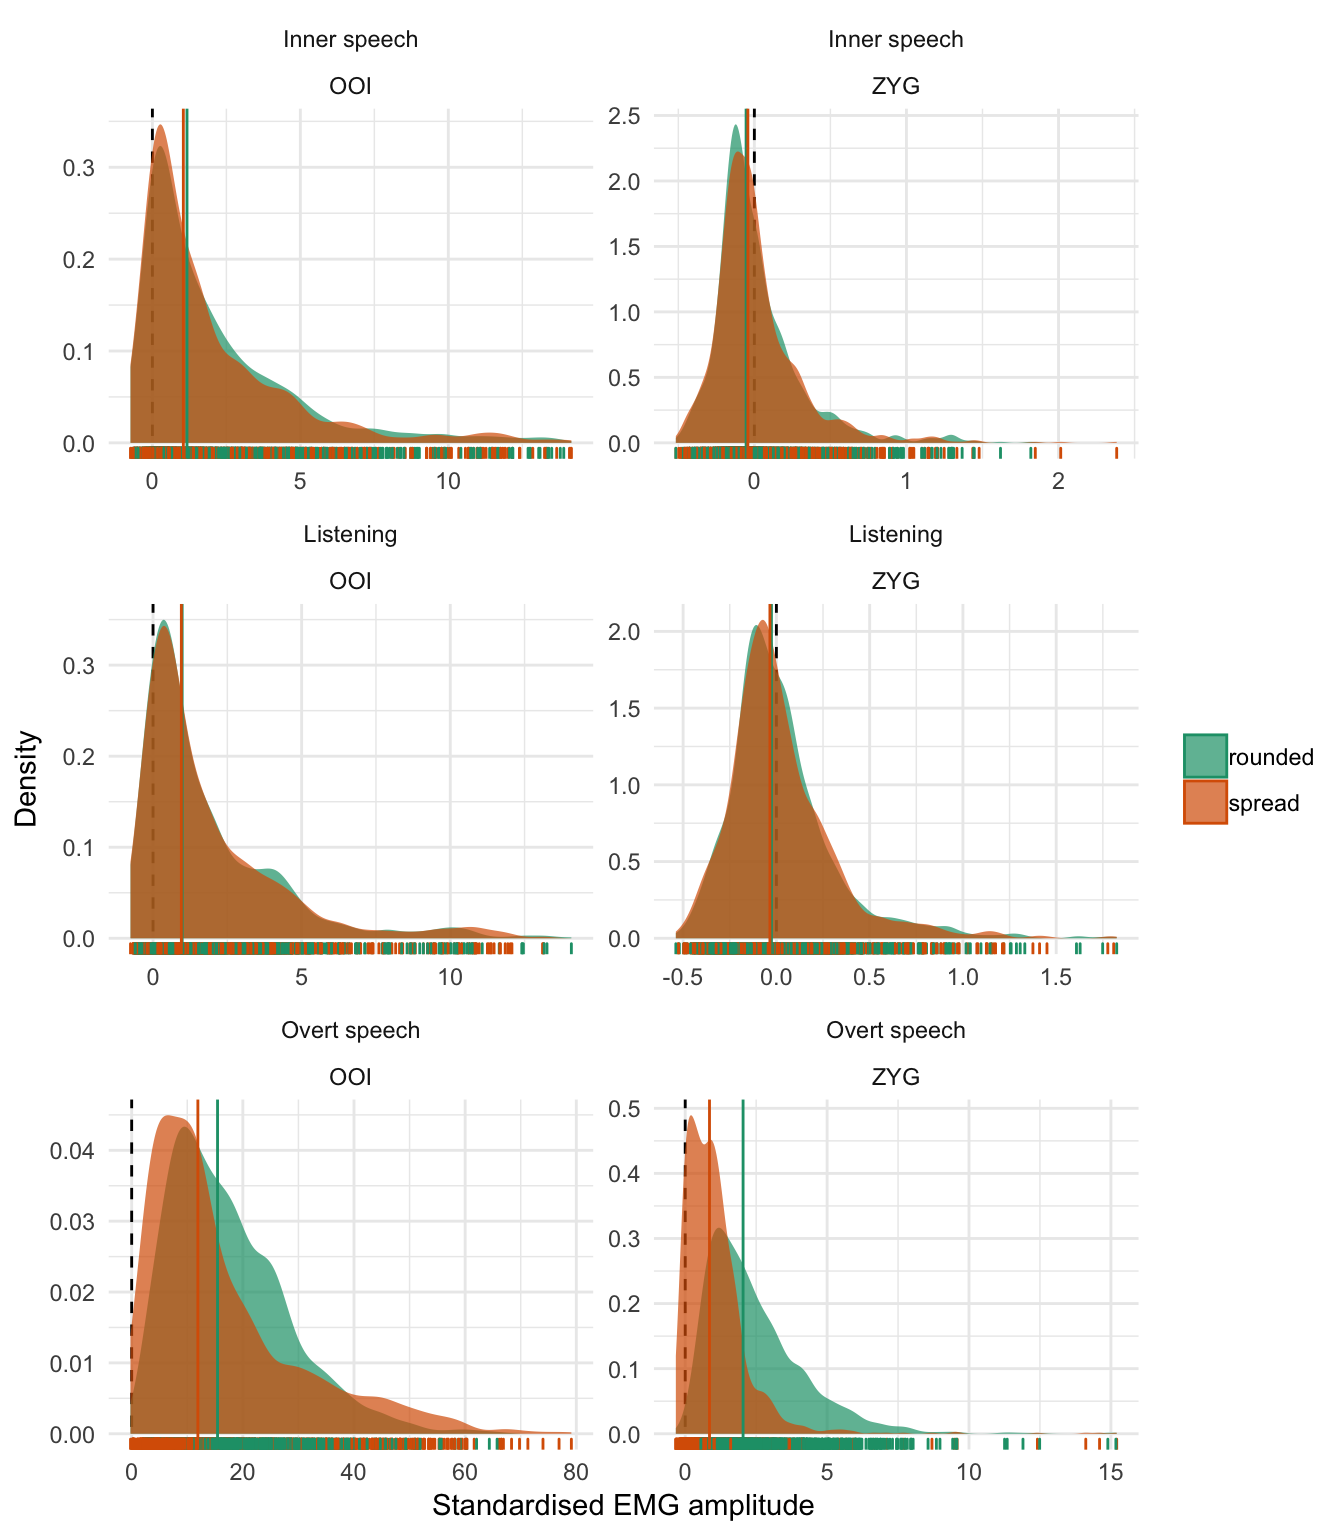
\includegraphics[width=1\linewidth]{05-chap5_files/figure-latex/generalplot-1} 

}

\caption{Distribution of standardised EMG scores by class and by muscle. The first row corresponds to the inner speech condition, the second one to the listening condition, and the third one to the overt speech condition. The first column depicts the EMG amplitude recorded over the OOI muscle while the second column represents the EMG amplitude recorded over the ZYG muscle. Each individual data point is represented as a vertical bar along the x-axis. The vertical coloured line represents the by-class median.}\label{fig:generalplot}
\end{figure}

\hypertarget{confirmatory-preregistered-analyses-1}{%
\subsection{Confirmatory (preregistered) analyses}\label{confirmatory-preregistered-analyses-1}}

\hypertarget{bayesian-multivariate-multilevel-gaussian-model}{%
\subsubsection{Bayesian multivariate multilevel Gaussian model}\label{bayesian-multivariate-multilevel-gaussian-model}}

We then compared the standardised EMG amplitude \(\delta\) for each muscle in each condition (Overt Speech, Inner Speech, Listening) by fitting a multivariate multilevel Gaussian model (as detailed previously in the Methods section). We predicted an higher increase of OOI activity during the production of rounded items in comparison to spread items and conversely, a higher increase of ZYG activity during the inner production of rounded items in comparison to spread items. These predictions should also apply to the overt speech condition (and to the listening condition). We should not observe any by-class differences of FRO and COR activity in any condition.

\begin{table}[H]
\begin{center}
\begin{threeparttable}
\caption{\label{tab:outputbmod1}Estimates from the Gaussian BMLM concerning the OOI and the ZYG.}
\small{
\begin{tabular}{llllllll}
\toprule
Response & \multicolumn{1}{c}{Term} & \multicolumn{1}{c}{Estimate} & \multicolumn{1}{c}{SE} & \multicolumn{1}{c}{Lower} & \multicolumn{1}{c}{Upper} & \multicolumn{1}{c}{Rhat} & \multicolumn{1}{c}{BF01}\\
\midrule
OOI & Inner Speech & 1.87 & 0.42 & 1.02 & 2.66 & 1.00 & 0.02\\
OOI & Listening & 1.73 & 0.37 & 1.03 & 2.48 & 1.00 & 0.00\\
OOI & Overt Speech & 16.19 & 1.96 & 12.38 & 19.95 & 1.00 & 0.00\\
OOI & Inner Speech x Class & 0.11 & 0.19 & -0.28 & 0.47 & 1.00 & 43.73\\
OOI & Listening x Class & -0.14 & 0.27 & -0.67 & 0.38 & 1.00 & 32.53\\
OOI & Overt Speech x Class & 0.70 & 0.27 & 0.18 & 1.22 & 1.00 & 1.29\\
ZYG & Inner Speech & 0.01 & 0.04 & -0.07 & 0.10 & 1.00 & 237.72\\
ZYG & Listening & 0.02 & 0.04 & -0.06 & 0.10 & 1.00 & 218.90\\
ZYG & Overt Speech & 1.77 & 0.22 & 1.32 & 2.23 & 1.00 & 0.00\\
ZYG & Inner Speech x Class & 0.01 & 0.03 & -0.05 & 0.06 & 1.00 & 360.68\\
ZYG & Listening x Class & 0.00 & 0.04 & -0.08 & 0.08 & 1.00 & 263.36\\
ZYG & Overt Speech x Class & 1.35 & 0.04 & 1.27 & 1.42 & 1.00 & 0.00\\
\bottomrule
\addlinespace
\end{tabular}
}
\begin{tablenotes}[para]
\textit{Note.} For each muscle (response), the first three lines represent the estimated average
amplitude in each condition, and its standard error (SE).
The three subsequent rows represent the estimated average difference between the two classes
of nonwords in each condition (i.e., the interaction effect). The 'Lower' and 'Upper' columns
    contain the lower and upper bounds of the 95\% CrI, while the 'Rhat' column reports the Gelman-Rubin statistic.
    The last column reports the Bayes factor in favour of the null hypothesis (BF01).
\end{tablenotes}
\end{threeparttable}
\end{center}
\end{table}

The results of this model are summarised in Table \ref{tab:outputbmod1}. This table reports the estimated average EMG amplitude in each condition and the corresponding BF\footnote{As they are not the main focus of interest here and for the sake of clarity, descriptive results for the other two facial muscles and for the forearm muscle are reported in the supplementary materials.}. This analysis revealed that the EMG amplitude of the OOI was higher than baseline (the standardised score was above zero) in every condition whereas it was only the case in the overt speech condition for the ZYG. Crucially, we did not observe the hypothesised difference according to the class of nonwords on the OOI during inner speech production (\(\beta\) = 0.108, 95\% CrI {[}-0.281, 0.466{]}, BF\textsubscript{01} = 43.727) nor on the ZYG (\(\beta\) = 0.007, 95\% CrI {[}-0.047, 0.057{]}, BF\textsubscript{01} = 360.677).

Figure \ref{fig:predbmod1} depicts these results by representing the distribution of the raw data (coloured dots) along with the predictions from this model. The black dots and vertical intervals represent the predicted mean and associated 95\% credible interval for each class of non-word, each condition and for the OOI and the ZYG. Coherently with Table \ref{tab:outputbmod1}, this figure shows that the fitted model predicts no noticeable differences between the two classes of non-words in any condition for the OOI muscle. However, it predicts a higher average EMG amplitude associated with the rounded item as compared to the spread items in the overt speech condition for the ZYG muscle.

\begin{figure}[H]

{\centering 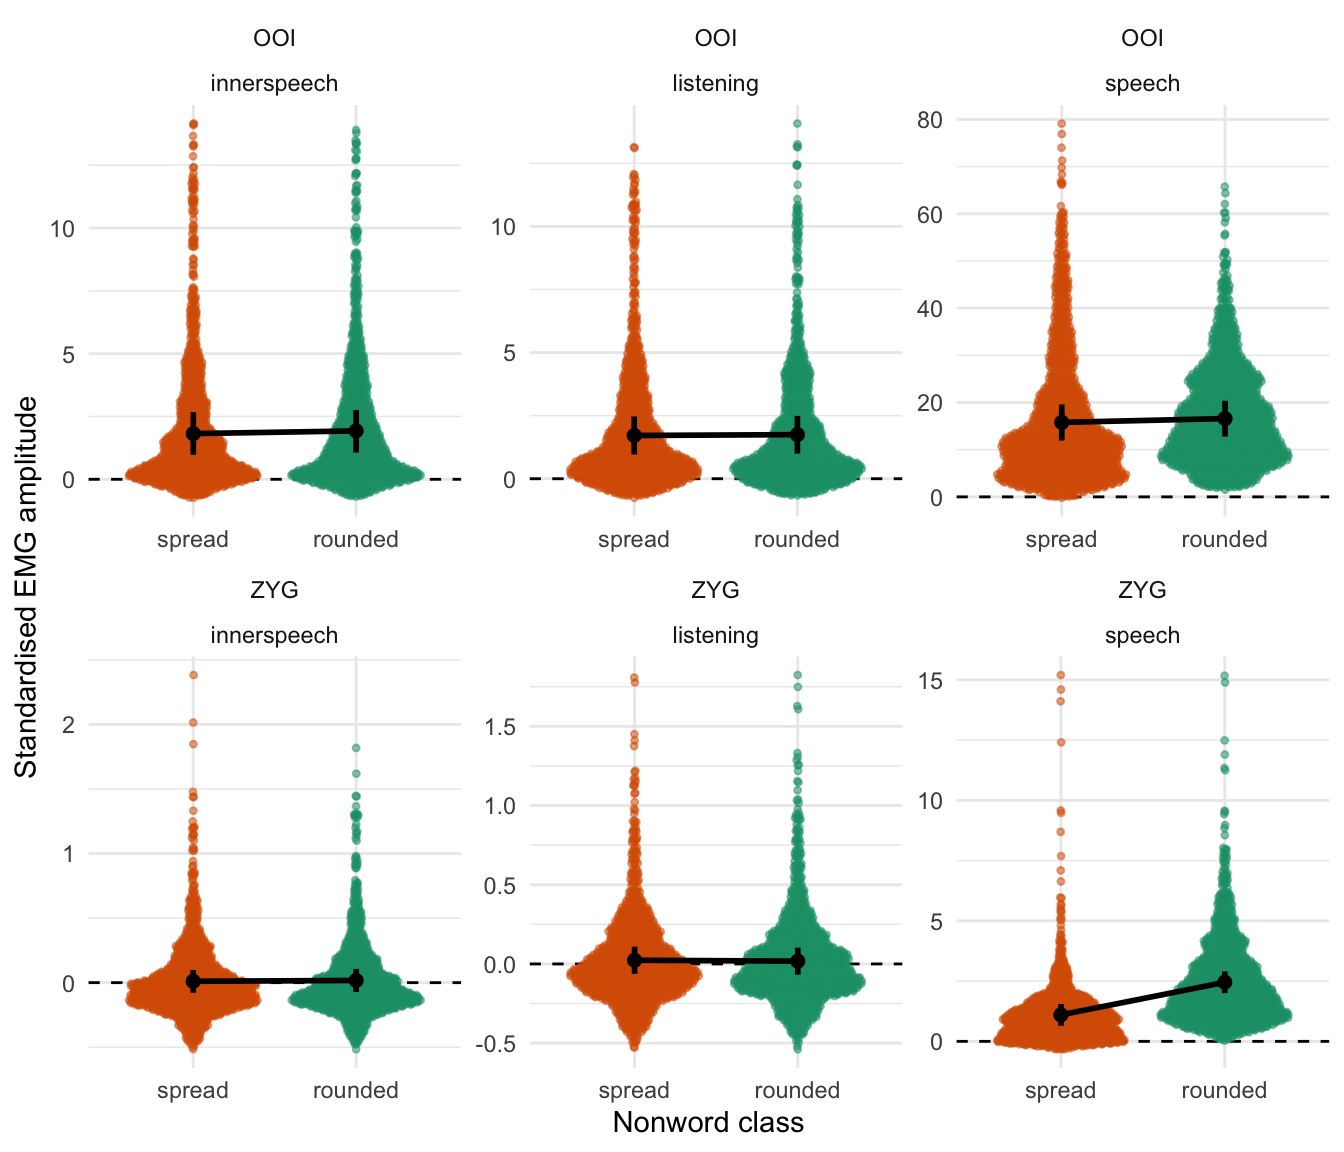
\includegraphics[width=1\linewidth]{05-chap5_files/figure-latex/predbmod1-1} 

}

\caption{Raw data along with posterior predictions of the first model for the OOI and the ZYG muscles. Dots represent the mean prediction of this model by condition, while the vertical error bars represent the 95\% credible intervals around the mean.}\label{fig:predbmod1}
\end{figure}

Before proceeding further with the interpretation of the results, it is essential to check the quality of this first model. A useful diagnostic of the model's predictive abilities is known as \emph{posterior predictive checking} (PPC) and consists in comparing observed data to data simulated from the posterior distribution (e.g., Gelman et al., \protect\hyperlink{ref-gelman_bayesian_2013}{2013}). The idea behind PPC is that a good model should be able to generate data that resemble the observed data (Gabry, Simpson, Vehtari, Betancourt, \& Gelman, \protect\hyperlink{ref-gabry_visualization_2019}{2019}). In this vein, Figure \ref{fig:ppcbmod1} represents the distribution of the whole dataset (across all participants and conditions) by muscle (the dark blue line) along with the distribution of hypothetical datasets generated from the posterior distribution of the model (the light blue lines). As can be seen from this Figure, the distributions of the data generated from the model differ considerably from the distribution of the observed data. Therefore, in the next section, we turn to a more appropriate model for these data.

\begin{figure}[H]

{\centering \includegraphics[width=1\linewidth]{05-chap5_files/figure-latex/ppcbmod1-1} 

}

\caption{Posterior predictive checking for the first model concerning the OOI and ZYG muscles. The dark blue line represents the distribution of the raw data (across all conditions) while light blue lines are dataset generated from the posterior distribution.}\label{fig:ppcbmod1}
\end{figure}

\hypertarget{bayesian-multivariate-multilevel-distributional-skew-normal-model}{%
\subsubsection{Bayesian multivariate multilevel distributional Skew-Normal model}\label{bayesian-multivariate-multilevel-distributional-skew-normal-model}}

The previous figure reveals an important failure of the first model, as it fails to generate data that look like the data we have collected. More precisely, the collected data look right-skewed, as it usually happens with physiological measurements. To improve on the Gaussian model, we then assume a Skew-normal distribution for the response variable (the standardised EMG amplitude \(\delta\)). The Skew-normal distribution is a generalisation of the Gaussian distribution with three parameters \(\xi\) (xi), \(\omega\) (omega), and \(\alpha\) (alpha) for location, scale, and shape (skewness), respectively\footnote{NB: the Gaussian distribution can be considered a special case of the Skew-normal distribution when \(\alpha = 1\).}. In addition, we also improve the first model by turning it into a \emph{distributional model}, that is, a model in which we can specify predictor terms for all parameters of the assumed response distribution (Bürkner, \protect\hyperlink{ref-R-brms}{2018}). More precisely, we use this approach to predict both the location, the scale, and the skewness of the Skew-Normal distribution (whereas the first model only allowed predicting the mean of a Gaussian distribution). As can been seen in Figure \ref{fig:ppcbmod3}, this second model seems better than the first one at generating data that look like the observed data.

\begin{figure}[H]

{\centering 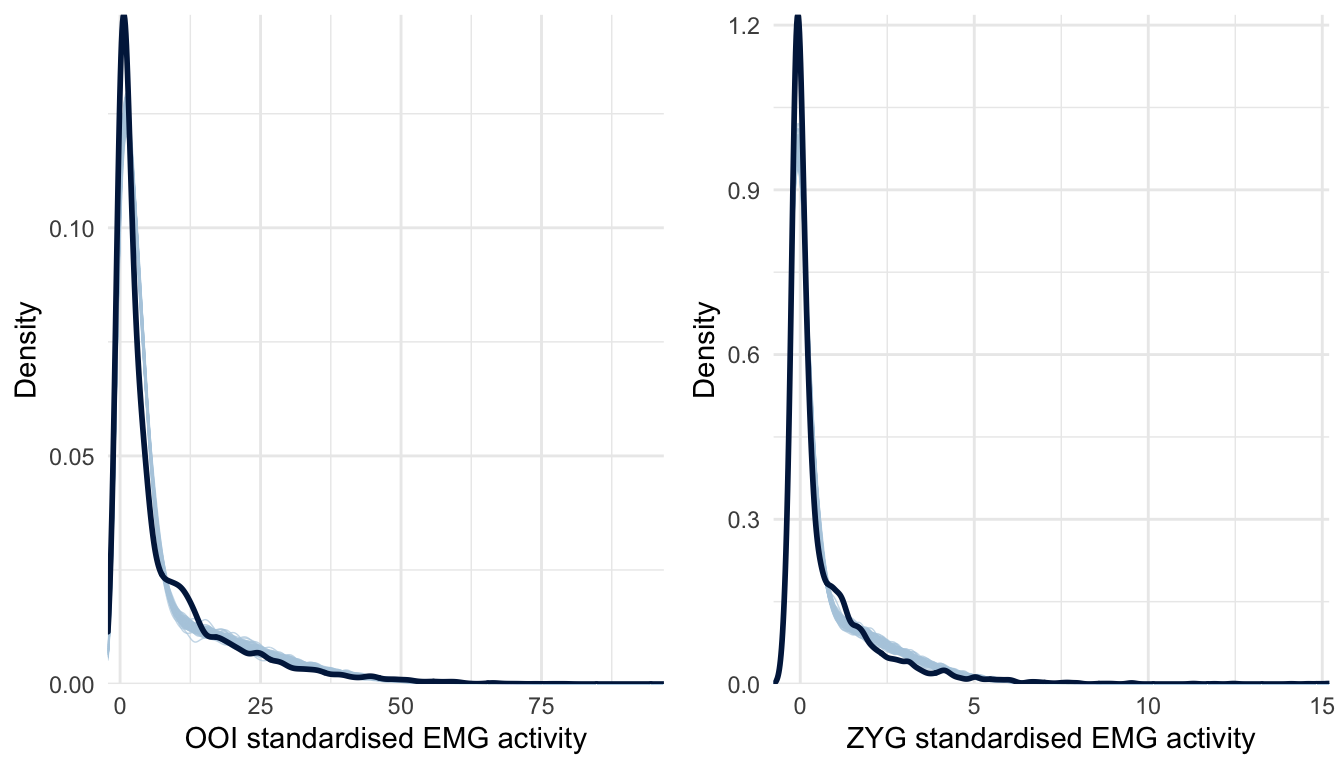
\includegraphics[width=1\linewidth]{05-chap5_files/figure-latex/ppcbmod3-1} 

}

\caption{Posterior predictive checking for the Skew-Normal model concerning the OOI and ZYG muscles. The dark blue line represents the distribution of the raw data while light blue lines are dataset generated from the posterior distribution.}\label{fig:ppcbmod3}
\end{figure}

\begin{table}[H]
\begin{center}
\begin{threeparttable}
\caption{\label{tab:outputbmod3}Estimates from the distributional Skew-Normal model concerning the OOI and the ZYG.}
\small{
\begin{tabular}{llllllll}
\toprule
Response & \multicolumn{1}{c}{Term} & \multicolumn{1}{c}{Estimate} & \multicolumn{1}{c}{SE} & \multicolumn{1}{c}{Lower} & \multicolumn{1}{c}{Upper} & \multicolumn{1}{c}{Rhat} & \multicolumn{1}{c}{BF01}\\
\midrule
OOI & Inner Speech & 2.35 & 0.04 & 2.28 & 2.44 & 1.00 & 0.00\\
OOI & Listening & 2.12 & 0.04 & 2.04 & 2.19 & 1.00 & 0.00\\
OOI & Overt Speech & 17.38 & 0.21 & 16.97 & 17.78 & 1.00 & 0.00\\
OOI & Inner Speech x Class & 0.04 & 0.03 & -0.02 & 0.10 & 1.00 & 118.39\\
OOI & Listening x Class & -0.02 & 0.04 & -0.09 & 0.06 & 1.00 & 237.23\\
OOI & Overt Speech x Class & 1.64 & 0.18 & 1.28 & 1.99 & 1.00 & 0.00\\
ZYG & Inner Speech & 0.04 & 0.00 & 0.02 & 0.04 & 1.00 & 0.00\\
ZYG & Listening & 0.04 & 0.01 & 0.03 & 0.05 & 1.00 & 0.00\\
ZYG & Overt Speech & 1.91 & 0.02 & 1.86 & 1.95 & 1.00 & 0.00\\
ZYG & Inner Speech x Class & 0.00 & 0.01 & -0.01 & 0.02 & 1.00 & 1,089.34\\
ZYG & Listening x Class & 0.00 & 0.01 & -0.02 & 0.02 & 1.00 & 856.03\\
ZYG & Overt Speech x Class & 0.64 & 0.03 & 0.58 & 0.70 & 1.00 & 0.00\\
\bottomrule
\addlinespace
\end{tabular}
}
\begin{tablenotes}[para]
\textit{Note.} For each muscle (response), the first three lines represent the estimated average
amplitude in each condition, and its standard error (SE).
The three subsequent rows represent the estimated average difference between the two classes
of nonwords in each condition (i.e., the interaction effect). The 'Lower' and 'Upper' columns
    contain the lower and upper bounds of the 95\% CrI, while the 'Rhat' column reports the Gelman-Rubin statistic.
    The last column reports the Bayes factor in favour of the null hypothesis (BF01).
\end{tablenotes}
\end{threeparttable}
\end{center}
\end{table}

The estimates of this second model are summarised in Table \ref{tab:outputbmod3} and Figure \ref{fig:predbmod3}. According to this model, the EMG amplitude of the OOI was higher than baseline (the estimated standardised score was above zero) in every condition whereas it was only the case in the overt speech condition for the ZYG. We did not observe the hypothesised difference according to the class of nonwords during inner speech production, neither on the OOI (\(\beta\) = 0.043, 95\% CrI {[}-0.015, 0.103{]}, BF\textsubscript{01} = 118.391) nor on the ZYG (\(\beta\) = 0.005, 95\% CrI {[}-0.011, 0.021{]}, BF\textsubscript{01} = 1089.341).

\begin{figure}[H]

{\centering 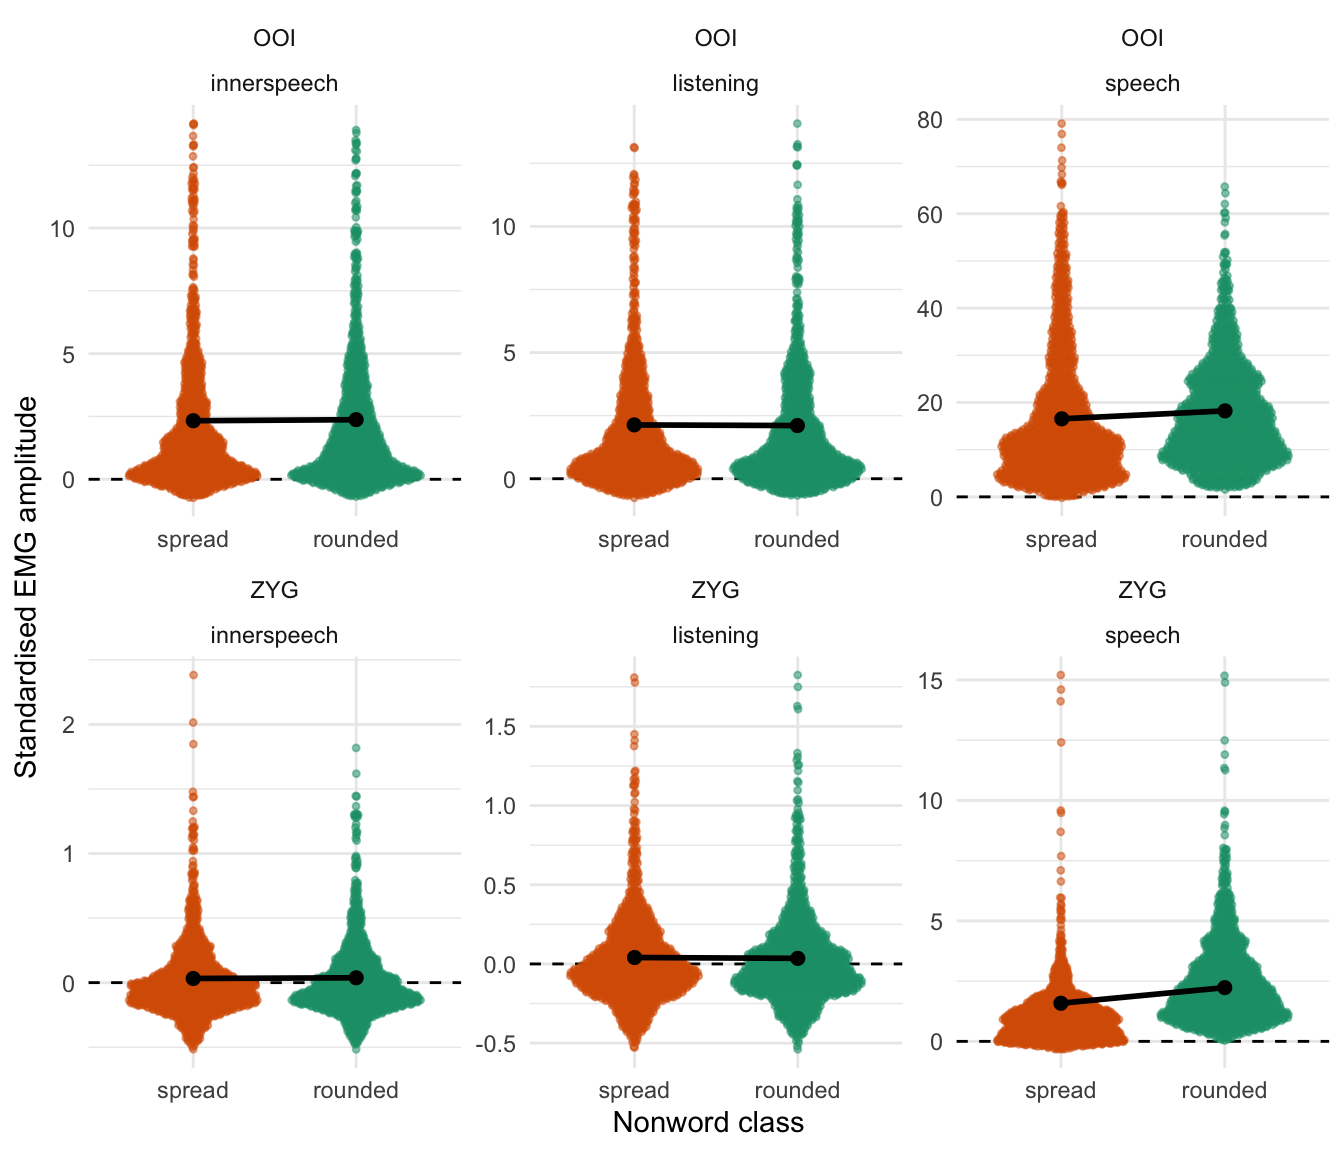
\includegraphics[width=1\linewidth]{05-chap5_files/figure-latex/predbmod3-1} 

}

\caption{Raw data along with posterior predictions of the third model for the OOI and the ZYG muscles. Dots represent the mean prediction of this model by condition (concerning the location parameter) whereas the vertical error bars represent the 95\% credible intervals.}\label{fig:predbmod3}
\end{figure}

Predictions from this model are visually represented in Figure \ref{fig:predbmod3}. This figure differs from Figure \ref{fig:predbmod1} (showing the predictions of the Gaussian model) in that the second model (the Skew-normal model) predicts shifts in location for both the OOI and the ZYG muscles according the class of non-word in overt speech prediction. In contrast, the first model (the Gaussian model) predicted a by-class difference only for the ZYG muscle.

\hypertarget{exploratory-non-preregistered-analyses}{%
\subsection{Exploratory (non-preregistered) analyses}\label{exploratory-non-preregistered-analyses}}

In the previous section, we tried to predict the average EMG amplitude by condition on each single muscle. Although this approach was appropriate to tackle our initial research question (i.e., can we distinguish muscle-specific EMG correlates of inner speech production?), it is not optimal to answer more general questions such as \enquote{can we predict the content of inner speech based on the available EMG data?}. In Figure \ref{fig:2Demg}, we depict the distribution of the by-word averaged EMG scores in the 2D space formed by the OOI and the ZYG muscles. This figure reveals that although different nonwords produced in overt speech seem difficult to discriminate on the basis of a single muscle (cf.~Figure \ref{fig:generalplot}), it seems easier to discriminate them in the space formed by two muscles (here OOI and ZYG). More precisely, the two classes of nonwords seem to form two separate clusters in the overt speech condition, but these clusters do not seem discriminable in the inner speech or in the listening condition.

\begin{figure}[H]

{\centering 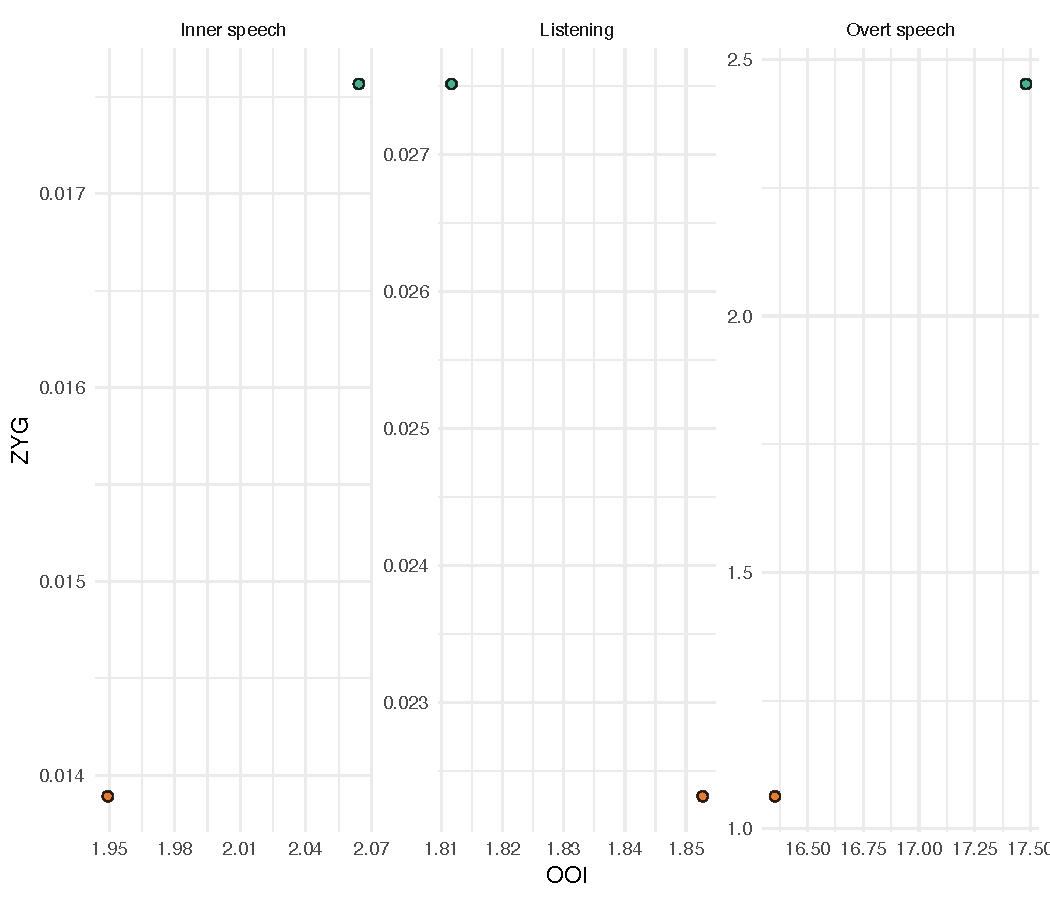
\includegraphics[width=1\linewidth]{05-chap5_files/figure-latex/2Demg-1} 

}

\caption{Average EMG amplitude for each nonword in each condition, in the two-dimensional space formed by the OOI and ZYG muscles.}\label{fig:2Demg}
\end{figure}

In other words, it is easier to discriminate these signals in the multidimensional space of all speech muscles, rather than by considering each muscle independently. Thus, we used a supervised machine learning algorithm aiming to classify speech signals according to the class of nonwords. Broadly, the machine learning approach seeks to find a relationship between an input \(X\) (e.g., EMG recordings over the four facial muscles) and an output \(Y\) (e.g., the class of nonwords). Once trained, it allows predicting a value of the output based on some input values, whose prediction can be evaluated against new observations.

We used a random forest algorithm, as implemented in the \texttt{caret} package (Jed Wing et al., \protect\hyperlink{ref-R-caret}{2018}). Random forests (RFs) represent an ensemble of many decision trees (a forest), which allow predictions to be made based on a series of decision rules (e.g., is the score on predictor \(x_{1}\) higher or lower than \(z\) ? If yes, then \ldots, if not, then \ldots). The specificity of RFs is to combine a large number of trees (usually above 100 trees), and to base the final conclusion on the average of these trees, thus preventing overfitting. We used three separate RFs to classify EMG signals in each condition (Overt Speech, Inner Speech, and Listening).

To evaluate the performance of this approach, we report the raw accuracy (along with its resampling-based 95\% confidence interval), or the proportion of data points in the test dataset for which the RF algorithm predicted the correct class of nonwords. First, we randomly split the entire dataset into a training (80\%) and a test set (20\%). The training set was used for the learning while the test set was used to evaluate the predictions of the algorithm. To prevent overfitting, we used repeated 10-fold cross-validation during the learning phase.

\hypertarget{predicting-the-class-of-nonwords-during-overt-speech-production}{%
\subsubsection{Predicting the class of nonwords during overt speech production}\label{predicting-the-class-of-nonwords-during-overt-speech-production}}

We first tried to predict the class of nonwords produced in overt speech, based on the activity of the four facial muscles (OOI, ZYG, COR, FRO). Each predictor was centred to its mean and standardised before the analysis.

\begin{table}[H]
\begin{center}
\begin{threeparttable}
\caption{\label{tab:CMovert}Confusion matrix with by-class error for the overt speech condition.}
\begin{tabular}{cccc}
\toprule
 & \multicolumn{2}{c}{Reference}  &\\
\cmidrule(r){2-3}
Prediction & \multicolumn{1}{c}{rounded} & \multicolumn{1}{c}{spread} & \multicolumn{1}{c}{class.error}\\
\midrule
rounded & 971 & 165 & 0.145\\
spread & 204 & 956 & 0.176\\
\bottomrule
\end{tabular}
\end{threeparttable}
\end{center}
\end{table}

This analysis revealed an overall classification accuracy of 0.841, 95\% CI {[}0.809, 0.87{]}. The relative importance of each feature (i.e., each muscle) for prediction is represented in Figure \ref{fig:VarImpOvert}.

\begin{figure}[H]

{\centering 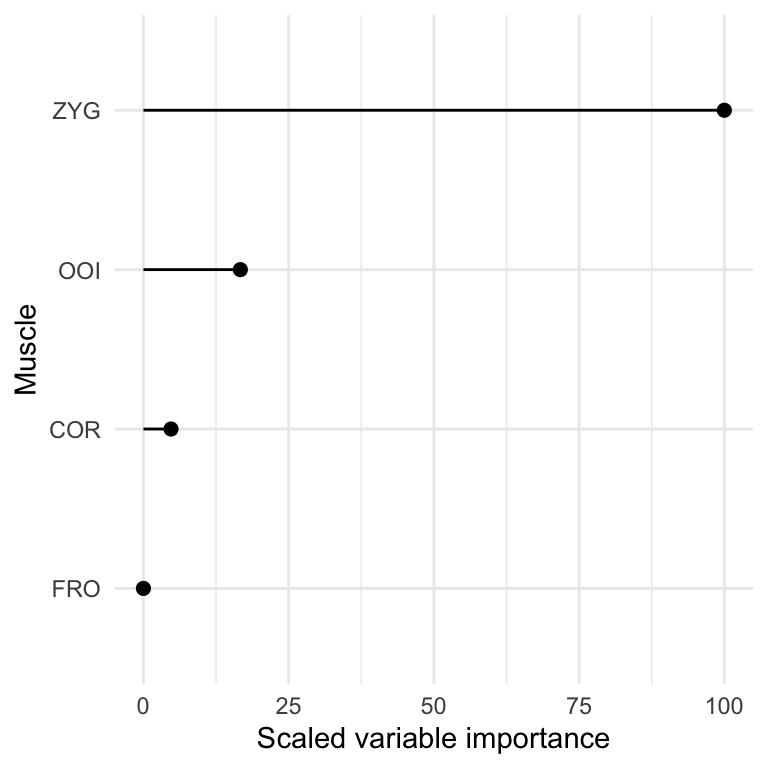
\includegraphics[width=1\linewidth]{05-chap5_files/figure-latex/VarImpOvert-1} 

}

\caption{Scaled variable importance for overt speech classification.}\label{fig:VarImpOvert}
\end{figure}

This figure reveals that the muscles containing most information to discriminate the two classes of nonwords are the ZYG and the OOI, whereas, as predicted, forehead muscles do not seem to strongly contribute to predictive accuracy during overt speech production.

\hypertarget{predicting-the-class-of-nonwords-during-inner-speech-production-and-listening}{%
\subsubsection{Predicting the class of nonwords during inner speech production and listening}\label{predicting-the-class-of-nonwords-during-inner-speech-production-and-listening}}

We then applied the same strategy (the same algorithm) to the signals recorded in the inner speech and listening conditions. The results of these analyses are reported in Table \ref{tab:CMinner} and Table \ref{tab:CMlistening}.

\begin{table}[H]
\begin{center}
\begin{threeparttable}
\caption{\label{tab:CMinner}Confusion matrix with by-class classification error for the inner speech condition.}
\begin{tabular}{cccc}
\toprule
 & \multicolumn{2}{c}{Reference}  &\\
\cmidrule(r){2-3}
Prediction & \multicolumn{1}{c}{rounded} & \multicolumn{1}{c}{spread} & \multicolumn{1}{c}{class.error}\\
\midrule
rounded & 460 & 550 & 0.545\\
spread & 517 & 532 & 0.493\\
\bottomrule
\end{tabular}
\end{threeparttable}
\end{center}
\end{table}

This analysis revealed an overall classification accuracy of 0.508, 95\% CI {[}0.464, 0.552{]} in the inner speech condition, which indicates that the RF algorithm did not allow discriminating the two classes of nonwords better than random guessing.

\begin{table}[H]
\begin{center}
\begin{threeparttable}
\caption{\label{tab:CMlistening}Confusion matrix with by-class classification error for the listening condition.}
\begin{tabular}{cccc}
\toprule
 & \multicolumn{2}{c}{Reference}  &\\
\cmidrule(r){2-3}
Prediction & \multicolumn{1}{c}{rounded} & \multicolumn{1}{c}{spread} & \multicolumn{1}{c}{class.error}\\
\midrule
rounded & 512 & 517 & 0.502\\
spread & 525 & 490 & 0.517\\
\bottomrule
\end{tabular}
\end{threeparttable}
\end{center}
\end{table}

This analysis similarly revealed an overall classification accuracy of 0.488, 95\% CI {[}0.444, 0.533{]} in the listening condition.

\hypertarget{discussion-2}{%
\section{Discussion}\label{discussion-2}}

With this study we aimed to replicate and extend previous findings showing that facial electromyography can be used to discriminate inner speech content (e.g., McGuigan \& Dollins, \protect\hyperlink{ref-mcguigan_patterns_1989}{1989}; McGuigan \& Winstead, \protect\hyperlink{ref-mcguigan_discriminative_1974}{1974}). As these studies used small samples of children, our study aimed to examine whether such results can be reproduced using surface electromyography and modern signal processing methods in an adult sample.

To this end, it was crucial to first show that the EMG correlates of our two classes of nonwords were discriminable during overt speech production. Surprisingly, the data we collected during overt speech production do not corroborate the hypothesis according to which the average EMG amplitude of the OOI should be higher during the production of \enquote{rounded} nonwords as compared to \enquote{spread} nonwords. For both orofacial speech muscles (OOI and ZYG), the average EMG amplitude was higher for rounded nonwords than for spread nonwords during overt speech production. Moreover, while the average EMG amplitude recorded over speech muscles was higher than baseline in both the inner speech and listening conditions, we did not find differences of activation according to the content of the material (the class of nonword). An automatic classification approach, using the four facial muscles, revealed that although it was possible to discriminate EMG signals related to the two classes of nonwords with a reasonable accuracy during overt speech production, this approach failed in discriminating these two classes during inner speech production or during listening. We also observed a higher EMG amplitude recorded over the facial (both orofacial and non-orofacial) muscles during inner speech production and during the listening of speech production than during rest. However, as pinpointed by Garrity (\protect\hyperlink{ref-garrity_electromyography_1977}{1977}), this observation is not sufficient to conclude that these activations were actually related to inner speech production, because i) both orofacial speech-related muscles and forehead non-speech related muscles showed similar EMG amplitude changes from baseline and ii) we did not observe different changes in EMG amplitude depending on the content of inner speech (i.e., depending on the class of nonword to be uttered).

Before discussing the theoretical implications of these results, two main issues are worth discussing. First, how can we explain that rounded nonwords were associated with higher EMG amplitude during overt speech on both OOI and ZYG muscles? Second, how can we explain the indiscriminability of inner speech content, which seems to contradict classic as well as recent findings in the field (e.g., Kapur et al., \protect\hyperlink{ref-kapur_alterego_2018}{2018})? We turn to each of these questions in the following.

To answer the first question, we began by comparing our results to results obtained by another group (Eskes et al., \protect\hyperlink{ref-eskes_predicting_2017}{2017}). The authors of this study recorded surface EMG activity from five participants while they were producing seven facial expressions and five isolated vowel sounds (/a/, /e/, /i/, /o/, /u/). They recorded EMG activity over eight facial muscles (the zygomaticus major (ZYG), the risorius (RIS), the orbicularis oris superior (OOS) and inferior (OOI), the mentalis (MEN), the depressor anguli oris (DAO), the levator labii superioris (LLS) muscles, and the digastric muscle (DIG)). We divided these vowels in two classes to fit our own classes of nonwords. More precisely, we have created the following two classes: a \emph{rounded} class, composed of the vowels /o/ and /u/, and a \emph{spread} class, composed of the vowels /e/ and /i/\footnote{We did not include the vowel /a/ because it theoretically does not fit in one of these two categories.}. We present the average EMG amplitude recorded over the OOI and the ZYG according to the vowel class in Table \ref{tab:eskes}.

\begin{table}[H]
\begin{center}
\begin{threeparttable}
\caption{\label{tab:eskes}Standardised EMG amplitude recorded over the OOI and the ZYG during overt speech production of rounded versus spread vowels in Eskes et al. (2017).}
\begin{tabular}{ccccccc}
\toprule
Muscle & \multicolumn{1}{c}{Item} & \multicolumn{1}{c}{Observations} & \multicolumn{1}{c}{Mean} & \multicolumn{1}{c}{SD} & \multicolumn{1}{c}{Median} & \multicolumn{1}{c}{Histogram}\\
\midrule
OOI & rounded & 50 & 59.7 & 60.09 & 42.03 & ▇▃▂▁▁▁▁▁\\
OOI & spread & 50 & 22.15 & 11.92 & 20.65 & ▇▆▇▂▂▂▁▁\\
ZYG & rounded & 50 & 7.39 & 3.78 & 6.27 & ▇▅▃▁▁▁▁▁\\
ZYG & spread & 50 & 10.15 & 6.2 & 7.99 & ▇▆▂▂▁▁▁▁\\
\bottomrule
\addlinespace
\end{tabular}
\begin{tablenotes}[para]
\textit{Note.} The number of observations is given by the number of vowels to be pronunced in each category (2) times the number of repetitions (5) times the number of participants (5), for a total of 50 observations per cell. 
\end{tablenotes}
\end{threeparttable}
\end{center}
\end{table}

We notice that Eskes et al. (\protect\hyperlink{ref-eskes_predicting_2017}{2017}) have indeed observed the dissociation we initially predicted, that is, that the EMG amplitude recorded over the OOI was higher during the pronunciation of rounded vowels than during pronunciation of spread vowels, while the reverse pattern was observed concerning the ZYG\footnote{Paired-samples Wilcoxon signed rank tests revealed a significant shift in location (pseudomedian) between rounded and spread items for the OOI (\(\beta\) = 24.12, 95\% CI {[}15.19, 40.77{]}, V = 1184, p \textless{} .001) with rounded items being associated with a higher location than spread items. This analysis revealed a significant shift in the inverse direction concerning the ZYG (\(\beta\) = -1.51, 95\% CI {[}-2.94, -0.48{]}, V = 275, p \textless{} .001).}. However, one crucial difference between Eskes et al. (\protect\hyperlink{ref-eskes_predicting_2017}{2017}) design and ours is the complexity of the linguistic material. Whereas Eskes et al. (\protect\hyperlink{ref-eskes_predicting_2017}{2017}) used single phonemes, we chose to use bisyllabic nonwords to increase the ecological validity of the paradigm. Although these nonwords were specifically created to theoretically increase the engagement of either the OOI or the ZYG (see section \ref{nonwords}), it is reasonable to expect differences in the average EMG amplitude between the phoneme and the (non)word level. More precisely, we expect the \emph{average} EMG amplitude associated with the production of a given phoneme (e.g., /y/) to be impacted by the production of the consonant (e.g., /b/) it is paired with, due to coarticulation. More generally, we could hypothesise that the difference between the \emph{average} EMG amplitude recorded during the production of the phoneme /i/ and during the production of the phoneme /y/ could be reduced when these phonemes are coarticulated in CV or CVCV sequences like /byby/ or /didi/. In other words, we might expect an interaction effect between the structure of the to-be produced speech sequence (either a single vowel or a CV/CVCV sequence) and the class of the vowel. This is coherent with previous findings showing that the muscular activity associated with vowels production is strongly influenced by the surrounding consonants in CVC sequences (e.g., Fromkin, \protect\hyperlink{ref-fromkin_neuro-muscular_1966}{1966}). Thus, further investigations should focus on how the average EMG amplitude is impacted by coarticulation during the production of CVCV sequences.

With regards to inner speech, our results do not support theoretical predictions of the \emph{motor simulation view}, according to which it should be possible to discriminate classes of nonwords produced in inner speech based on EMG signals. Whereas this outcome is consistent with some recent results (Meltzner et al., \protect\hyperlink{ref-meltzner_speech_2008}{2008})\footnote{The authors of this study were able to obtain high classification accuracies during both overt and mouthed speech but not during covert speech, despite the fact that they used eleven sensors on the neck and the lower face. However, words were only repeated three times, which might have lead to poor sensitivity. Interestingly and despite the lack of peripheral muscular activation during covert speech, they have observed similar respiratory activity between overt and covert speech, echoing previous findings (e.g., Conrad \& Schönle, \protect\hyperlink{ref-conrad_speech_1979}{1979}).}, it also stands in sharp contrast with classical results in the field (e.g., McGuigan \& Dollins, \protect\hyperlink{ref-mcguigan_patterns_1989}{1989}; McGuigan \& Winstead, \protect\hyperlink{ref-mcguigan_discriminative_1974}{1974}) as well as more recent developments. For instance, Kapur et al. (\protect\hyperlink{ref-kapur_alterego_2018}{2018}) developed a wearable device composed of seven surface EMG sensors that can attain a 92\% median classification accuracy in discriminating internally vocalised digits. There are a few crucial differences between Kapur et al. (\protect\hyperlink{ref-kapur_alterego_2018}{2018})'s work and ours that stand as good candidates to explain the discrepancies between our results. First, the strategy adopted to position the sensors was radically different. Following guidelines from the field of psychophysiology, our strategy was to position sensors precisely over the facial muscles of interest, aligned with the direction of the muscle fibers and in theoretically optimal positions to record activity of this muscle while reducing cross-talk. However, precisely because of pervasive cross-talk in facial surface EMG recordings, this strategy, whereas maximising the probability of recording activity from a given single muscle, was also (as a result) reducing the probability of recording activity from potentially speech-relevant neighbour muscles. Therefore, this strategy might work sub-optimally when the goal of the experiment is to extract the maximum amount of (relevant) EMG information to discriminate inner speech content. However, this problem might be mitigated by using more sensors and a more lenient sensor-positioning approach. Whereas we recorded the EMG amplitude over only two lower facial muscles (OOI and ZIG), Kapur et al. (\protect\hyperlink{ref-kapur_alterego_2018}{2018}) analysed EMG data from seven different sensors, whose position and number was defined iteratively in order to maximise the classification accuracy. In other words, the parameters of the experiment were iteratively optimised to maximise a certain outcome (classification accuracy). This strategy is radically different from the classical approach in experimental and cognitive psychology where experimental conditions are defined to test theoretically derived hypotheses. Whereas the first approach is arguably more efficient at solving a particular problem at hand, the second approach might be more efficient in tackling theoretical questions. For instance, a recent study reported a greater EMG amplitude of laryngeal and lip muscles during auditory verbal tasks (covert singing) than during visual imagery tasks (Pruitt, Halpern, \& Pfordresher, \protect\hyperlink{ref-pruitt_covert_2018}{2018}). By coupling EMG recording with demographic and psychological measures, they were able to show that these correlates were related to the level of accuracy in singing, thus shedding light upon the nature and functions of peripheral muscular activity during covert singing.

Putting aside considerations related to methodological aspects of the present study, these results do not corroborate the \emph{motor simulation view} of inner speech production. Instead, it seems to support the \emph{abstraction view}, which postulates that inner speech results from the activation of abstract linguistic representations. However, individual differences in discriminability highlight that the abstractness of inner speech might be flexible (Oppenheim \& Dell, \protect\hyperlink{ref-oppenheim_motor_2010}{2010}). Indeed, although for most participants it was not possible to discriminate the content of inner speech, it was possible to discriminate the content of inner speech for two of them (S\_15 and S\_17). This suggests either that the extent to which inner speech production recruits the speech motor system might vary between individuals or that it might vary within individual depending on the properties of the ongoing task (these two suggestions are not mutually exclusive). For instance, we know from early research on the EMG correlates of inner speech that the average amplitude of these correlates tend to be higher when the task is more difficult (i.e., requires more effort, Sokolov, \protect\hyperlink{ref-sokolov_inner_1972}{1972}). As such, the extent to which inner speech production recruits the speech motor system could be moderated by manipulating the difficulty of the ongoing task. In addition, we know that the electromyographic activity recorded during motor imagery could be moderated by the perspective taken in motor imagery. A distinction is made between first-person perspective or \emph{internal imagery} (i.e., imagining an action as we would execute it) and third-person perspective or \emph{external imagery} (i.e., imagining an action as an observer of this action), that seem to involve different neural and cognitive processes. It has been shown that a first-person perspective generally results in greater EMG activity than motor imagery in a third-person perspective (Hale, \protect\hyperlink{ref-hale_effects_1982}{1982}; Harris \& Robinson, \protect\hyperlink{ref-harris_effects_1986}{1986}). Moreover, the first-person perspective tends to be associated with more kinaesthetic feelings than the third-person one (which relies more heavily on visual percepts). While the perspective issue does not apply to inner speech production, we hypothesise that involvement of the speech motor system during inner speech production may be moderated by the specific instructions given to the participants. For instance, by instructing participants to focus on \emph{inner speaking} (imagining speaking), instead of \emph{inner hearing} (imagining hearing), and by asking them to focus on the kinaesthetic feelings related to speech acts (rather than on auditory percepts), we would expect to find a higher average EMG amplitude recorded over the speech muscles.

Of course, the current study and the above discussion should be interpreted with a few words of caution in mind. Although the number of observations reported in the present study is reasonable\footnote{For each class of nonwords, we collected around 6 x 10 = 60 observations by condition and by participant. For 26 participants and two classes of nonwords, this results in 26 (participants) x 120 (individual trials) x 3 (conditions) = 9360 observations. However, after rejecting trials with movement artefacts, we had 7997 observations in total.}, the sensibility of the experiment could be improved by increasing the number of observations and/or by reducing two important sources of variation. More precisely, one could reduce the variance related to the item (the specific nonword being uttered) by selecting nonwords that are more similar to each other in the way they are uttered, by selecting less items or simpler items. Similarly, particular attention should be devoted to reducing inter-participant variability, which could be done by using more guided and specific instructions, as well as a longer training phase to familiarise the participant with the task.

In summary, we have demonstrated that while surface electromyography may lead to reasonable accuracy in discriminating classes of nonwords during overt speech production (using signals recorded over only two speech-related muscles), it did not permit to discriminate these two classes during inner speech production. These results, in comparison with results obtained by other teams (e.g., Kapur et al., \protect\hyperlink{ref-kapur_alterego_2018}{2018}), highlight that depending on the aim of the research, different strategies might be more or less successfully pursued. More precisely, if the goal is to attain high classification accuracy (problem-solving approach), then the parameters of the experiment (e.g., number of repetitions, number of sensors, position of the sensors, parameters of the signal processing workflow) should be optimised based on the desired outcome (i.e., classification accuracy). However, the classical laboratory strategy used in experimental and cognitive psychology, aiming to compare specific conditions (or muscles) to each other in a controlled environment, is deemed to be more appropriate when the aim of the research is to sharpen our understanding of the psychological phenomenon under study.

\hypertarget{suppCh5}{%
\section{Supplementary materials}\label{suppCh5}}

Pre-registered protocol, open data, as well as reproducible code and figures are available at \url{https://osf.io/czer4}.

Aside from previously cited packages, several other packages have been used for the writing of this paper, among which the \texttt{ggrepel} and \texttt{ggplot2} packages for plotting (Slowikowski, \protect\hyperlink{ref-R-ggrepel}{2018}; Wickham et al., \protect\hyperlink{ref-R-ggplot2}{2018}) as well as the \texttt{tidyverse}, \texttt{sjstats}, \texttt{here}, \texttt{skimr}, and \texttt{glue} packages for code writing and formatting (Hester, \protect\hyperlink{ref-R-glue}{2017}; Lüdecke, \protect\hyperlink{ref-R-sjstats}{2018}; McNamara, Arino de la Rubia, Zhu, Ellis, \& Quinn, \protect\hyperlink{ref-R-skimr}{2018}; Müller, \protect\hyperlink{ref-R-here}{2017}; Wickham, \protect\hyperlink{ref-R-tidyverse}{2017}).

\hypertarget{acknowledgements-2}{%
\section{Acknowledgements}\label{acknowledgements-2}}

This project was funded by the ANR project INNERSPEECH (grant number ANR-13-BSH2-0003-01). The first author of this manuscript is funded by a fellowship from Univ. Grenoble Alpes.

\newpage

\begin{vplace}[1]

\begin{summary}{Summary of Chapter\getcurrentref{chapter}}

In this chapter, we examined the reliability of our EMG measurements to detect peripheral muscular activity during inner speech production. To this end, we asked participants to produce two lists of nonwords, that were designed to induce either a strong activation of the lip muscles or a strong activation of the zygomaticus major muscle. We recorded the EMG amplitude of several facial muscles (including the orbicularis oris inferior and the zygomaticus major muscles) during the production of these nonwords in inner speech, overt speech, and during the listening of these nonwords. Based on previous results in the literature, we hypothesised that surface EMG may be used to discriminate the content (here, the class of nonword) produced in inner speech. However, an automatic classification revealed that although we were able to discriminate content produced in overt speech, we were not able to discriminate the content produced in inner speech based on surface EMG measurements. This result stands in contrast with previous historical results but also with more recent results obtained by other teams. However, crucial differences between other studies and ours include differences in the material used (e.g., surface vs. intramuscular recordings), the population (e.g., children vs. adults), or the general methodology (e.g., hypothesis testing vs. classification and optimisation). Despite this surprising result and the failure of the surface EMG methodology to "decode" the content of inner speech, the abundance of positive results in the literature still speaks in favour of the peripheral muscular components of inner speech and that it is possible to assess it using surface EMG. However, in order to avoid this potential limitation, we shifted in the second part of the present work to another strategy in examining the role of motor processes in rumination. More precisely, instead of recording peripheral muscular activation of induced rumination, in the next two chapters we try to directly interfere with the speech motor system to check whether this would affect verbal rumination.

\end{summary}

\end{vplace}

\hypertarget{chap6}{%
\chapter{Articulatory suppression effects on induced rumination}\label{chap6}}

\initial{T}his study explores whether the speech motor system is involved in verbal rumination. The motor simulation hypothesis considers inner speech as an action on its own, accompanied by simulated speech percepts, that would as such involve the speech motor system. If so, we could expect verbal rumination --as a particular kind of inner speech-- to be disrupted by concurrent involvement of the speech muscles. We recruited 106 healthy adults and measured their self-reported level of rumination before and after a rumination induction, as well as after five minutes of a subsequent motor task (either an articulatory suppression -silent mouthing- task or a finger tapping control task). We also evaluated to what extent ruminative thoughts were experienced with a verbal quality or in another modality (e.g., visual images, non-speech sounds). Self-reported levels of rumination showed a decrease after both motor activities (silent mouthing and finger-tapping), with only a slightly stronger decrease after the articulatory suppression than the control task. The rumination level decrease was not moderated by the modality of the ruminative thoughts. We discuss these results within the framework of verbal rumination as simulated speech and suggest alternative ways to test the engagement of the speech motor system in verbal rumination.\footnote{This experimental chapter is a submited manuscript reformatted for the need of this thesis. Pre-registered protocol, preprint, data, as well as reproducible code and figures are available at: \url{https://osf.io/3bh67/}.}

\hypertarget{introduction-3}{%
\section{Introduction}\label{introduction-3}}

A large part of our inner conscious experience involves verbal content, with internal monologues and conversations. Inner speech is considered as a major component of conscious experience and cognition (Hubbard, \protect\hyperlink{ref-hubbard_auditory_2010}{2010}; Hurlburt et al., \protect\hyperlink{ref-Hurlburt2013}{2013}; Klinger \& Cox, \protect\hyperlink{ref-klinger_dimensions_1987}{1987}). An important issue concerns the format and nature of inner speech and whether it is better described as a mere evocation of abstract amodal verbal representations or as a concrete motor simulation of actual speech production (for review, see Alderson-Day \& Fernyhough, \protect\hyperlink{ref-alderson-day_inner_2015}{2015}; Lœvenbruck et al., \protect\hyperlink{ref-loevenbruck_cognitive_2018}{2018}; Perrone-Bertolotti et al., \protect\hyperlink{ref-Perrone-Bertolotti2014}{2014}). In the first case, inner speech is seen as divorced from bodily experience, and includes, at most, faded auditory representations. In the second case, inner speech is considered as a physical process that unfolds over time, leading to an enactive re-creation of auditory a well as articulatory percepts. The latter hypothesis is interesting in the context of persistent negative and maladaptive forms of inner speech, such as rumination. If this hypothesis is correct, we could expect rumination --as a particular type of inner speech-- to be disrupted by concurrent involvement of the speech muscles. The present study aims at testing this specific idea.

Introspective explorations of the characteristics of inner speech have led to different views on the relative importance of its auditory and articulatory components, and on the involvement of motor processes. It has been suggested successively that speech motor representations would be purely motoric (Stricker, \protect\hyperlink{ref-stricker_studien_1880}{1880}), that they would be expressed dominantly in an auditory format (Egger, \protect\hyperlink{ref-egger_parole_1881}{1881}), or that they would consist in a mix of these in the overall population (Ballet, \protect\hyperlink{ref-ballet_langage_1886}{1886}). The intuitive distinction between auditory and motor phenomena is referred to in contemporary research by the terms of \emph{inner ear} and \emph{inner voice}, in line with Baddeley's classic model of working memory (e.g., Baddeley et al., \protect\hyperlink{ref-baddeley_exploring_1984}{1984}; see also Buchsbaum, \protect\hyperlink{ref-buchsbaum_role_2013}{2013}). Baddeley's model relies on a partnership between an \emph{inner ear} (i.e., storage) and an \emph{inner voice} (i.e., subvocal rehearsal), which can be highlighted by selectively blocking either one of these components (e.g., Smith, Wilson, \& Reisberg, \protect\hyperlink{ref-smith_role_1995}{1995}).

Empirical arguments supporting the crucial role of the inner voice in verbal working memory (subvocal articulatory rehearsal) and auditory imagery can be found in studies using articulatory suppression, in which the \emph{action} component (i.e., the \emph{inner voice}) of inner speech is disrupted. Articulatory suppression usually refers to a task which requires participants to utter speech sounds (or to produce speech gestures without sound), so that this activity disrupts ongoing speech production processes. Articulatory suppression can be produced with different degrees of vocalisation, going from overt uttering of irrelevant words, to whispering, mouthing (i.e., silent articulation), and simple clamping of the speech articulators. Many studies have shown that articulatory suppression can be used to disrupt the subvocal rehearsal mechanism of verbal working memory and --as a consequence-- impair the recall of verbal material (e.g., Baddeley et al., \protect\hyperlink{ref-baddeley_exploring_1984}{1984}; Larsen \& Baddeley, \protect\hyperlink{ref-larsen_disruption_2003}{2003}).

Inner speech has also been extensively studied from the perspective of psycholinguistics. Based on the study of errors accompanying the covert production of tongue twisters, inner speech has been suggested to be impoverished (as compared to overt speech) and to miss phonological detail (e.g., Oppenheim \& Dell, \protect\hyperlink{ref-oppenheim_inner_2008}{2008}, \protect\hyperlink{ref-oppenheim_motor_2010}{2010}). More precisely, these studies shown the phonemic similarity effect (the tendency to exchange phonemes with similar articulatory features) to be absent in inner speech. In contrast to these results, however, Corley et al. (\protect\hyperlink{ref-corley_error_2011}{2011}) found the phonemic similarity effect to be present in inner speech, suggesting that inner speech is not necessarily impoverished at the articulatory level.

In a study aiming at investigating the role of \emph{covert enactment} in auditory imagery, Reisberg, Smith, Baxter, \& Sonenshine (\protect\hyperlink{ref-reisberg_enacted_1989}{1989}) observed that the verbal transformation effect (Warren \& Gregory, \protect\hyperlink{ref-warren_auditory_1958}{1958}), namely the alteration of speech percepts when certain speech sounds are uttered in a repetitive way, also occurred during inner speech (although the verbal transformation effect was smaller than during overt speech), but was suppressed by concurrent articulation (e.g., chewing) or clamping the articulators. The fact that the verbal transformation effect was observed during inner speech and that it was reduced by concurrent chewing, even in inner speech, speaks in favour of the view of inner speech as an enacted simulation of overt speech.

Another piece of evidence for the effect of articulatory suppression on inner speech comes from a recent study by Topolinski \& Strack (\protect\hyperlink{ref-topolinski_motormouth_2009}{2009}) on the mere exposure effect, namely the fact that repeated exposure to a stimulus influences the evaluation of this stimulus in a positive way (Zajonc, \protect\hyperlink{ref-zajonc_attitudinal_1968}{1968}). Topolinski and Strack's study showed that the mere exposure effect for visually presented verbal material could be completely suppressed by blocking subvocal rehearsal (i.e., inner speech) when asking participants to chew a gum. The effect was preserved, however, when participants kneaded a soft ball with their hand (Topolinski \& Strack, \protect\hyperlink{ref-topolinski_motormouth_2009}{2009}). This finding suggests that blocking speech motor simulation interfered with the inner rehearsal of the visually presented verbal stimuli, thereby destroying the positive exposure effect. It provides additional experimental support to the view that inner speech involves a motor component.

The occurrence of motor simulation during inner speech is further backed by several studies using physiological measures to evaluate inner speech production properties. Using electrodes inserted in the tongue tip or lips of five participants, Jacobson (\protect\hyperlink{ref-jacobson_electrical_1931}{1931}) was able to detect electromyographic (EMG) activity during several tasks requiring inner speech. Similarly, Sokolov (\protect\hyperlink{ref-sokolov_inner_1972}{1972}) recorded intense lip and tongue muscle activation when participants had to perform complex tasks that necessitated substantial inner speech production (e.g., problem solving). Another study using surface electromyography (sEMG) demonstrated an increase in activity of the lip muscles during silent recitation tasks compared to rest, but no increase during the non-linguistic visualisation task (Livesay et al., \protect\hyperlink{ref-livesay_covert_1996}{1996}). An increase in the lip and forehead muscular activity has also been observed during induced rumination (Nalborczyk et al., \protect\hyperlink{ref-nalborczyk_orofacial_2017}{2017}). Furthermore, this last study also suggested that speech-related muscle relaxation was slightly more efficient in reducing subjective levels of rumination than non speech-related muscle relaxation, suggesting that relaxing or inhibiting the speech muscles could disrupt rumination.

Rumination is a \enquote{class of conscious thoughts that revolve around a common instrumental theme and that recur in the absence of immediate environmental demands requiring the thoughts} (Martin \& Tesser, \protect\hyperlink{ref-Martin}{1996}). Despite the fact that depressed patients report positive metacognitive beliefs about ruminating, which is often seen as a coping strategy in order to regulate mood (e.g., Papageorgiou \& Wells, \protect\hyperlink{ref-papageorgiou_metacognitive_2001}{2001}), rumination is known to significantly worsen mood (e.g., Moberly \& Watkins, \protect\hyperlink{ref-Moberly2008}{2008}; Nolen-Hoeksema \& Morrow, \protect\hyperlink{ref-nolen-hoeksema_effects_1993}{1993}), impair cognitive flexibility (e.g., Davis \& Nolen-Hoeksema, \protect\hyperlink{ref-Davis2000}{2000}; Lyubomirsky et al., \protect\hyperlink{ref-Lyubomirsky1998}{1998}), and to lead toward pronounced social exclusion and more interpersonal distress (Lam, Schuck, Smith, Farmer, \& Checkley, \protect\hyperlink{ref-lam_response_2003}{2003}). Although partly visual, rumination is a predominantly verbal process (Goldwin \& Behar, \protect\hyperlink{ref-goldwin_concreteness_2012}{2012}; McLaughlin et al., \protect\hyperlink{ref-mclaughlin_effects_2007}{2007}) and can therefore be considered as a maladaptive type of inner speech. In a study on worry, another form of repetitive negative thinking, Rapee (\protect\hyperlink{ref-rapee_utilisation_1993}{1993}) observed a \emph{tendency} for articulatory suppression, but not for visuo-spatial tasks, to produce some interference with worrying. He concluded that worry involves the phonological aspect of the central executive of working memory. We further add that, since repeating a word seems to reduce the ability to worry, this study suggests that articulatory aspects are at play during worry.

In this context, the question we addressed in this study is whether verbal rumination consists of purely abstract verbal representations or whether it is better described as a motor simulation of speech production, engaging the speech apparatus. If the latter hypothesis is correct, rumination experienced in verbal form (in contrast to a non-verbal form) should be disrupted by mouthing (i.e., silent articulation), and should not be disrupted by a control task that does not involve speech muscles (e.g., finger-tapping). Specifically, we thus sought to test the hypotheses that rumination could be disrupted by articulatory suppression (but not by finger-tapping), and that this disruption would be more pronounced when rumination is experienced in a verbal form than in a non-verbal form.

\hypertarget{methods-3}{%
\section{Methods}\label{methods-3}}

In the \emph{Methods} and \emph{Data analysis} sections, we report how we determined our sample size, all data exclusions, all manipulations, and all measures in the study (Simmons et al., \protect\hyperlink{ref-simmons_21_2012}{2012}). A pre-registered version of our protocol can be found on OSF: \url{https://osf.io/3bh67/}.

\hypertarget{sample}{%
\subsection{Sample}\label{sample}}

We originally planned for 128 participants to take part in the study. This sample size was set on the basis of results obtained by Topolinski \& Strack (\protect\hyperlink{ref-topolinski_motormouth_2009}{2009}), who observed an effect size around \(\eta_{p}^{2}=.06\). We expected a similar effect size for the current rumination disruption, since rumination can be conceived of as a subtype of inner speech\footnote{In the original power calculations included in the OSF preregistration platform, we had inadequately specified the effect size in GPower, but we only realised this erroneous specification after the freezing of the preregistration on the OSF platform. Therefore, the current sample size slightly differs from the preregistered one.}.

As we anticipated drop-out of participants due to our inclusion criteria (see below), a total of 184 undergraduate students in psychology from Univ. Grenoble Alpes took part in this experiment, in exchange for course credits. They were recruited via mailing list, online student groups, and posters. Each participant provided a written consent and this study was approved by the local ethics committee (CERNI N° 2016-05-31-9). To be eligible, participants had to be between 18 and 35 years of age, with no history of motor, neurological, psychiatric, or speech-development disorders. All participants spoke French as their mother tongue. After each participant gave their written consent, they completed the Center for Epidemiologic Studies - Depression scale (CES-D; Radloff, \protect\hyperlink{ref-radloff_ces-d_1977}{1977}). The CES-D is a 12-item questionnaire, validated in French (Morin et al., \protect\hyperlink{ref-morin_psychometric_2011}{2011}), aiming to assess the level of depressive symptoms in a subclinical population. Participants exceeding the threshold of clinical depressive symptoms (i.e., \textgreater23 for females and \textgreater17 for males; Radloff, \protect\hyperlink{ref-radloff_ces-d_1977}{1977}) were not included in the study for ethical reasons (N = 26).

To investigate articulatory suppression effects in the context of rumination, a successful induction of rumination is a prerequisite. Therefore, analyses were only conducted on participants who showed an effect of the rumination induction (i.e., strictly speaking, participants who reported more rumination after the induction than before). We thus discarded participants who did not show any increase in rumination level (N = 52, 32.91\% of total sample). The final sample comprised 106 participants (Mean age = 20.3018868, SD = 2.5728064, Min-Max = 18-31, 96 females).

\hypertarget{material-3}{%
\subsection{Material}\label{material-3}}

The experiment was programmed with OpenSesame software (Mathôt et al., \protect\hyperlink{ref-mathot_opensesame_2012}{2012}) and stimuli were displayed on a DELL latitude E6500 computer screen.

\hypertarget{questionaires}{%
\subsubsection{Questionaires}\label{questionaires}}

To control for confounding variables likely to be related to the intensity of the induction procedure, we administered the French version of the Positive and Negative Affect Schedule (PANAS; Watson, Clark, \& Tellegen, \protect\hyperlink{ref-watson_development_1988}{1988}), adapted to French by Gaudreau, Sanchez, \& Blondin (\protect\hyperlink{ref-Gaudreau2006}{2006}). This questionnaire includes 20 items, from which we can compute an overall index of both positive (by summing the scores on 10 positive items, thereafter \emph{PANASpos}) and negative affect (\emph{PANASneg}) at baseline. This questionnaire was administered at baseline. In order to evaluate trait rumination, at the end of the experiment participants completed the short version of the Ruminative Response Scale (RRS-R, Treynor et al., \protect\hyperlink{ref-treynor_rumination_2003}{2003}), validated in French (Douilliez, Guimpel, Baeyens, \& Philippot, \emph{in preparation}). From this questionnaire, scores on two dimensions were analysed (\emph{RRSbrooding} and \emph{RRSreflection}).

\hypertarget{measures}{%
\subsubsection{Measures}\label{measures}}

Measures of state rumination were recorded using a Visual Analogue Scale (VAS) previously used in Nalborczyk et al. (\protect\hyperlink{ref-nalborczyk_orofacial_2017}{2017}). This scale measured the degree of agreement with the sentence \enquote{At this moment, I am brooding on negative things} (translated from French), on a continuum between \enquote{Not at all} and \enquote{A lot} (afterwards coded between 0 and 100). This scale is subsequently referred to as the \emph{RUM} scale. It was used three times in the experiment, at baseline (after training but before the experiment started), after rumination induction, and after a motor task.

Additionally, participants answered questions about the modality of the thoughts that occurred while performing the motor task. This last questionnaire consisted of one question evaluating the occurrence frequency of different modalities of inner thoughts (e.g., visual imagery, verbal thoughts, music). Then, a verbal/non-verbal ratio (i.e., the score on the verbal item divided by the mean of the score on the non-verbal items) was computed, hereafter referred to as the \emph{Verbality} continuous predictor (this scale is available online: \url{https://osf.io/3bh67/}).

\hypertarget{tasks}{%
\subsubsection{Tasks}\label{tasks}}

In the first part of the experiment, ruminative thoughts were induced using a classical induction procedure. Then a motor task was executed. Participants were randomly allocated to one of two conditions. In the \emph{Mouthing} condition, the task consisted of repetitively making mouth opening-closing movements at a comfortable pace. This condition was selected as it is commonly used in articulatory suppression studies (e.g., Baddeley et al., \protect\hyperlink{ref-baddeley_exploring_1984}{1984}). As a control, a finger-tapping condition was used (the \emph{Tapping} condition), that consisted of tapping on the desk with the index finger of the dominant hand at a comfortable pace.

Although finger-tapping tasks are generally considered as good control conditions when using speech motor tasks, since they are comparable in terms of general attentional demands, it may be that orofacial gestures are intrinsically more complex than manual gestures (i.e., more costly, Emerson \& Miyake, \protect\hyperlink{ref-emerson_role_2003}{2003}). To discard the possibility that orofacial gestures (related to the \emph{Mouthing} condition) would be cognitively more demanding than manual ones (related to the \emph{Tapping} condition), we designed a pretest experiment in order to compare the two interference motor tasks used in the main experiment. Results of this control experiment showed no difference on reaction times during a visual search task between the two interference tasks (i.e., mouthing and finger-tapping). Full details are provided in Appendix \ref{appendix-eyetracking}.

\hypertarget{procedure-3}{%
\subsection{Procedure}\label{procedure-3}}

The experiment took place individually in a quiet and dimmed room. The total duration of the session ranged between 35min and 40min. Before starting the experiment, participants were asked to perform the motor task during 1 min, while following a dot moving at a random pace on the screen in front of them. This task was designed to train the participants to perform the motor task adequately. Following this training and after describing the experiment, the experimenter left the room and each participant had to fill-in a baseline questionnaire (adaptation of PANAS, see above) presented on the computer screen. Baseline state rumination was then evaluated using the \emph{RUM} scale. The whole experiment was video-monitored using a Sony HDR-CX240E video camera, in order to check that the participants effectively completed the task.

\hypertarget{rumination-induction-1}{%
\subsubsection{Rumination induction}\label{rumination-induction-1}}

Rumination induction consisted of two steps. The first step consisted of inducing a negative mood in order to enhance the effects of the subsequent rumination induction. Participants were asked to recall a significant personal failure experienced in the past five years. Then, participants were invited to evaluate the extent to which this memory was \enquote{intense for them} on a VAS between \enquote{Not at all} and \enquote{A lot}, afterwards coded between 0 and 100, and referred to as \emph{Vividness}.

The second step consisted of the rumination induction proper. We used a French translation of Nolen-Hoeksema \& Morrow (\protect\hyperlink{ref-nolen-hoeksema_effects_1993}{1993})'s rumination induction procedure. Participants had to read a list of 44 sentences related to the meaning, the causes and the consequences of their current affective or physiological state. Each phrase was presented on a computer screen for 10 seconds and the total duration of this step was 7 minutes and 20 seconds. State rumination was then evaluated again using the same VAS as the one used at baseline (\emph{RUM}).

\hypertarget{proc_supp}{%
\subsubsection{Motor task}\label{proc_supp}}

After the rumination induction, participants were asked to continue to think about \enquote{the meaning, causes, and consequences} of their feelings while either repetitively making mouth movements (for participants allocated in the \enquote{Mouthing} condition) or finger-tapping with the dominant hand for five minutes (for participants allocated in the \enquote{Tapping} condition). Afterwards, state rumination was again evaluated using the \emph{RUM} scale.

In order to evaluate trait rumination, participants completed the short version of the RRS (see above). Then were filled in the questionnaire on the modality of the thoughts that occurred while performing the motor task (see above). Figure \ref{fig:diagram} summarises the full procedure.

\begin{figure}[H]

{\centering 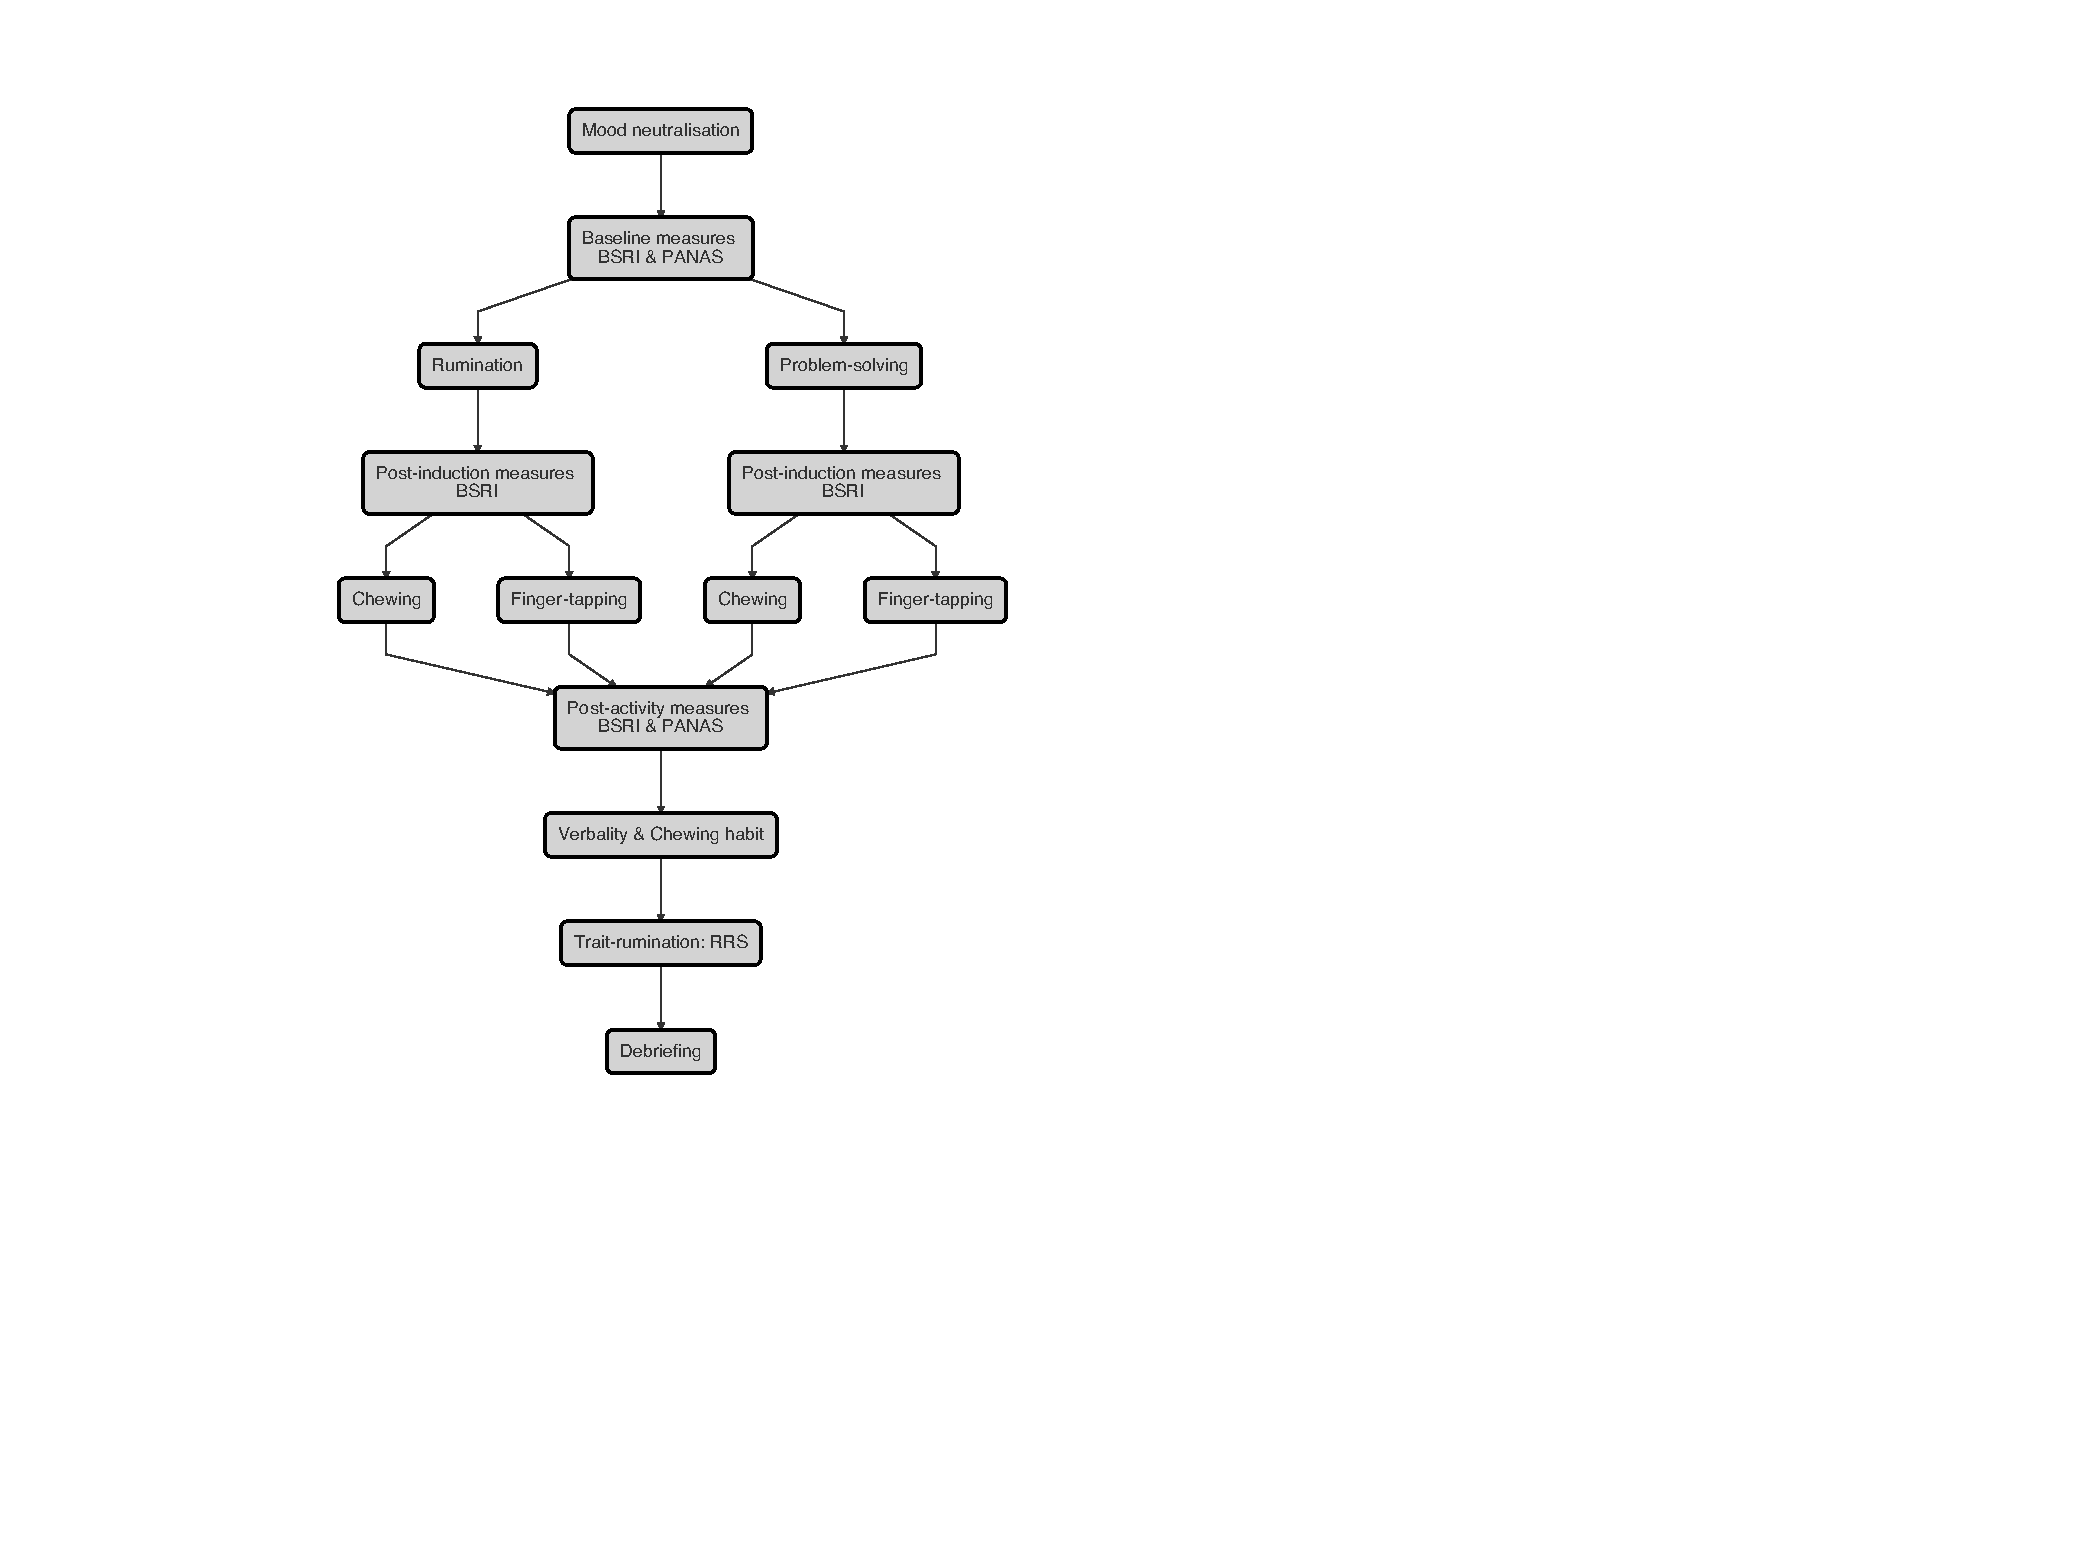
\includegraphics[width=1\linewidth]{06-chap6_files/figure-latex/diagram-1} 

}

\caption{Timeline of the experiment, from top to bottom.}\label{fig:diagram}
\end{figure}

\hypertarget{data-analysis-2}{%
\subsection{Data analysis}\label{data-analysis-2}}

Statistical analyses were conducted using R version 3.4.3 (R Core Team, \protect\hyperlink{ref-R-base}{2018}), and are reported with the \texttt{papaja} (Aust \& Barth, \protect\hyperlink{ref-R-papaja}{2018}) and \texttt{knitr} (Xie, \protect\hyperlink{ref-R-knitr}{2018}) packages.

\hypertarget{rumination-induction-2}{%
\subsubsection{Rumination induction}\label{rumination-induction-2}}

We centered and standardised each predictor in order to facilitate the interpretation of parameters. Data were then analysed using \emph{Induction} (2 modalities, before and after induction, contrast-coded) as a within-subject categorical predictor and \emph{RUM} as a dependent variable in a Bayesian multilevel linear model (BMLM), using the \texttt{brms} package (Bürkner, \protect\hyperlink{ref-R-brms}{2018})\footnote{An introduction to Bayesian statistics is outside the scope of this paper. However, the interested reader is referred to Nalborczyk et al. (\protect\hyperlink{ref-nalborczyk_introduction_2019}{2019}\protect\hyperlink{ref-nalborczyk_introduction_2019}{a}) for an introduction to Bayesian multilevel modelling using the \texttt{brms} package.}. This model was compared with more complex models including effects of control variables, such as baseline affect state (\emph{PANAS} scores) or the vividness of the memory chosen during the induction (\emph{Vividness} score).

Models were compared using the Widely Applicable Information Criterion (WAIC; Watanabe, \protect\hyperlink{ref-watanabe_asymptotic_2010}{2010}) --a generalisation of the Akaike information criterion (Akaike, \protect\hyperlink{ref-akaike_new_1974}{1974})-- and evidence ratios (Burnham \& Anderson, \protect\hyperlink{ref-burnham_model_2002}{2002}; Burnham, Anderson, \& Huyvaert, \protect\hyperlink{ref-burnham_aic_2011}{2011}; Hegyi \& Garamszegi, \protect\hyperlink{ref-hegyi_using_2011}{2011}). The WAIC provides a relative measure of predictive accuracy of the models (the WAIC is an approximation of the out-of-sample deviance of a model) and balances underfitting and overfitting by sanctioning models for their number of parameters. Evidence ratios (ERs) were computed as the ratios of weights: \(ER_{ij} = \dfrac{w_{i}}{w_{j}}\), where \(w_{i}\) and \(w_{j}\) are the Akaike weights of models \(i\) and \(j\), respectively. These weights can be interpreted as the probability of the model being the best model in terms of out-of-sample prediction (Burnham \& Anderson, \protect\hyperlink{ref-burnham_model_2002}{2002}). Whereas the use of WAIC is appropriate for model comparison and selection, it tells us nothing about the absolute fit of the model. To estimate this fit, we computed the Bayesian \(R^2\) for MLMs using the \texttt{bayes\_R2()} method in the brms package (Bürkner, \protect\hyperlink{ref-R-brms}{2018}).

Models were fitted using weakly informative priors (see the \protect\hyperlink{suppCh6}{supplementary materials} for code details). Two Markov Chain Monte-Carlo (MCMC) were ran for each model to approximate the posterior distribution, including each 5.000 iterations and a warmup of 2.000 iterations. Posterior convergence was assessed examining trace plots as well as the Gelman-Rubin statistic \(\hat{R}\). Constant effect estimates were summarised via their posterior mean and 95\% credible interval (CrI), where a credible interval can be considered as the Bayesian analogue of a classical confidence interval. When applicable, we also report Bayes factors (BFs), computed using the Savage-Dickey method, which consists in taking the ratio of the posterior density at the point of interest divided by the prior density at that point. These BFs can be interpreted as an updating factor, from prior knowledge (what we knew before seeing the data) to posterior knowledge (what we know after seeing the data).

\hypertarget{articulatory-suppression-effects}{%
\subsubsection{Articulatory suppression effects}\label{articulatory-suppression-effects}}

Data were analysed in the same fashion as in the first part of the experiment, using \emph{Session} (2 modalities, before and after motor activity, contrast-coded) as a within-subject categorical predictor, and \emph{Condition} (2 modalities, Mouthing and Tapping) as a between-subject categorical predictor and \emph{RUM} as a dependent variable.

\hypertarget{results-3}{%
\section{Results}\label{results-3}}

The results section follows the data analysis workflow. More precisely, for each part of the experiment (i.e., first the analysis of the induction effects and then, the analysis of the impact of mouthing vs.~finger-tapping), we first present the results of the model comparison stage in which we compare different models of increasing complexity. Subsequently, we report the estimates of the best model (the model with the lowest WAIC) and base our conclusions on this model.

\hypertarget{correlation-matrix-between-main-predictors-and-control-variables}{%
\subsection{Correlation matrix between main predictors and control variables}\label{correlation-matrix-between-main-predictors-and-control-variables}}

In order to prevent multicollinearity, we estimated the correlation between each pair of continuous predictors. Figure \ref{fig:correxp1} displays these correlations along with the marginal distribution of each variable. The absence of strong correlations (\(r > 0.8\)) between any of these variables suggests that they can each be included as control variables in the following statistical models. Summary statistics (mean and standard deviation) for all these variables can be found in Table \ref{tab:sumstat}.

\begin{figure}[H]
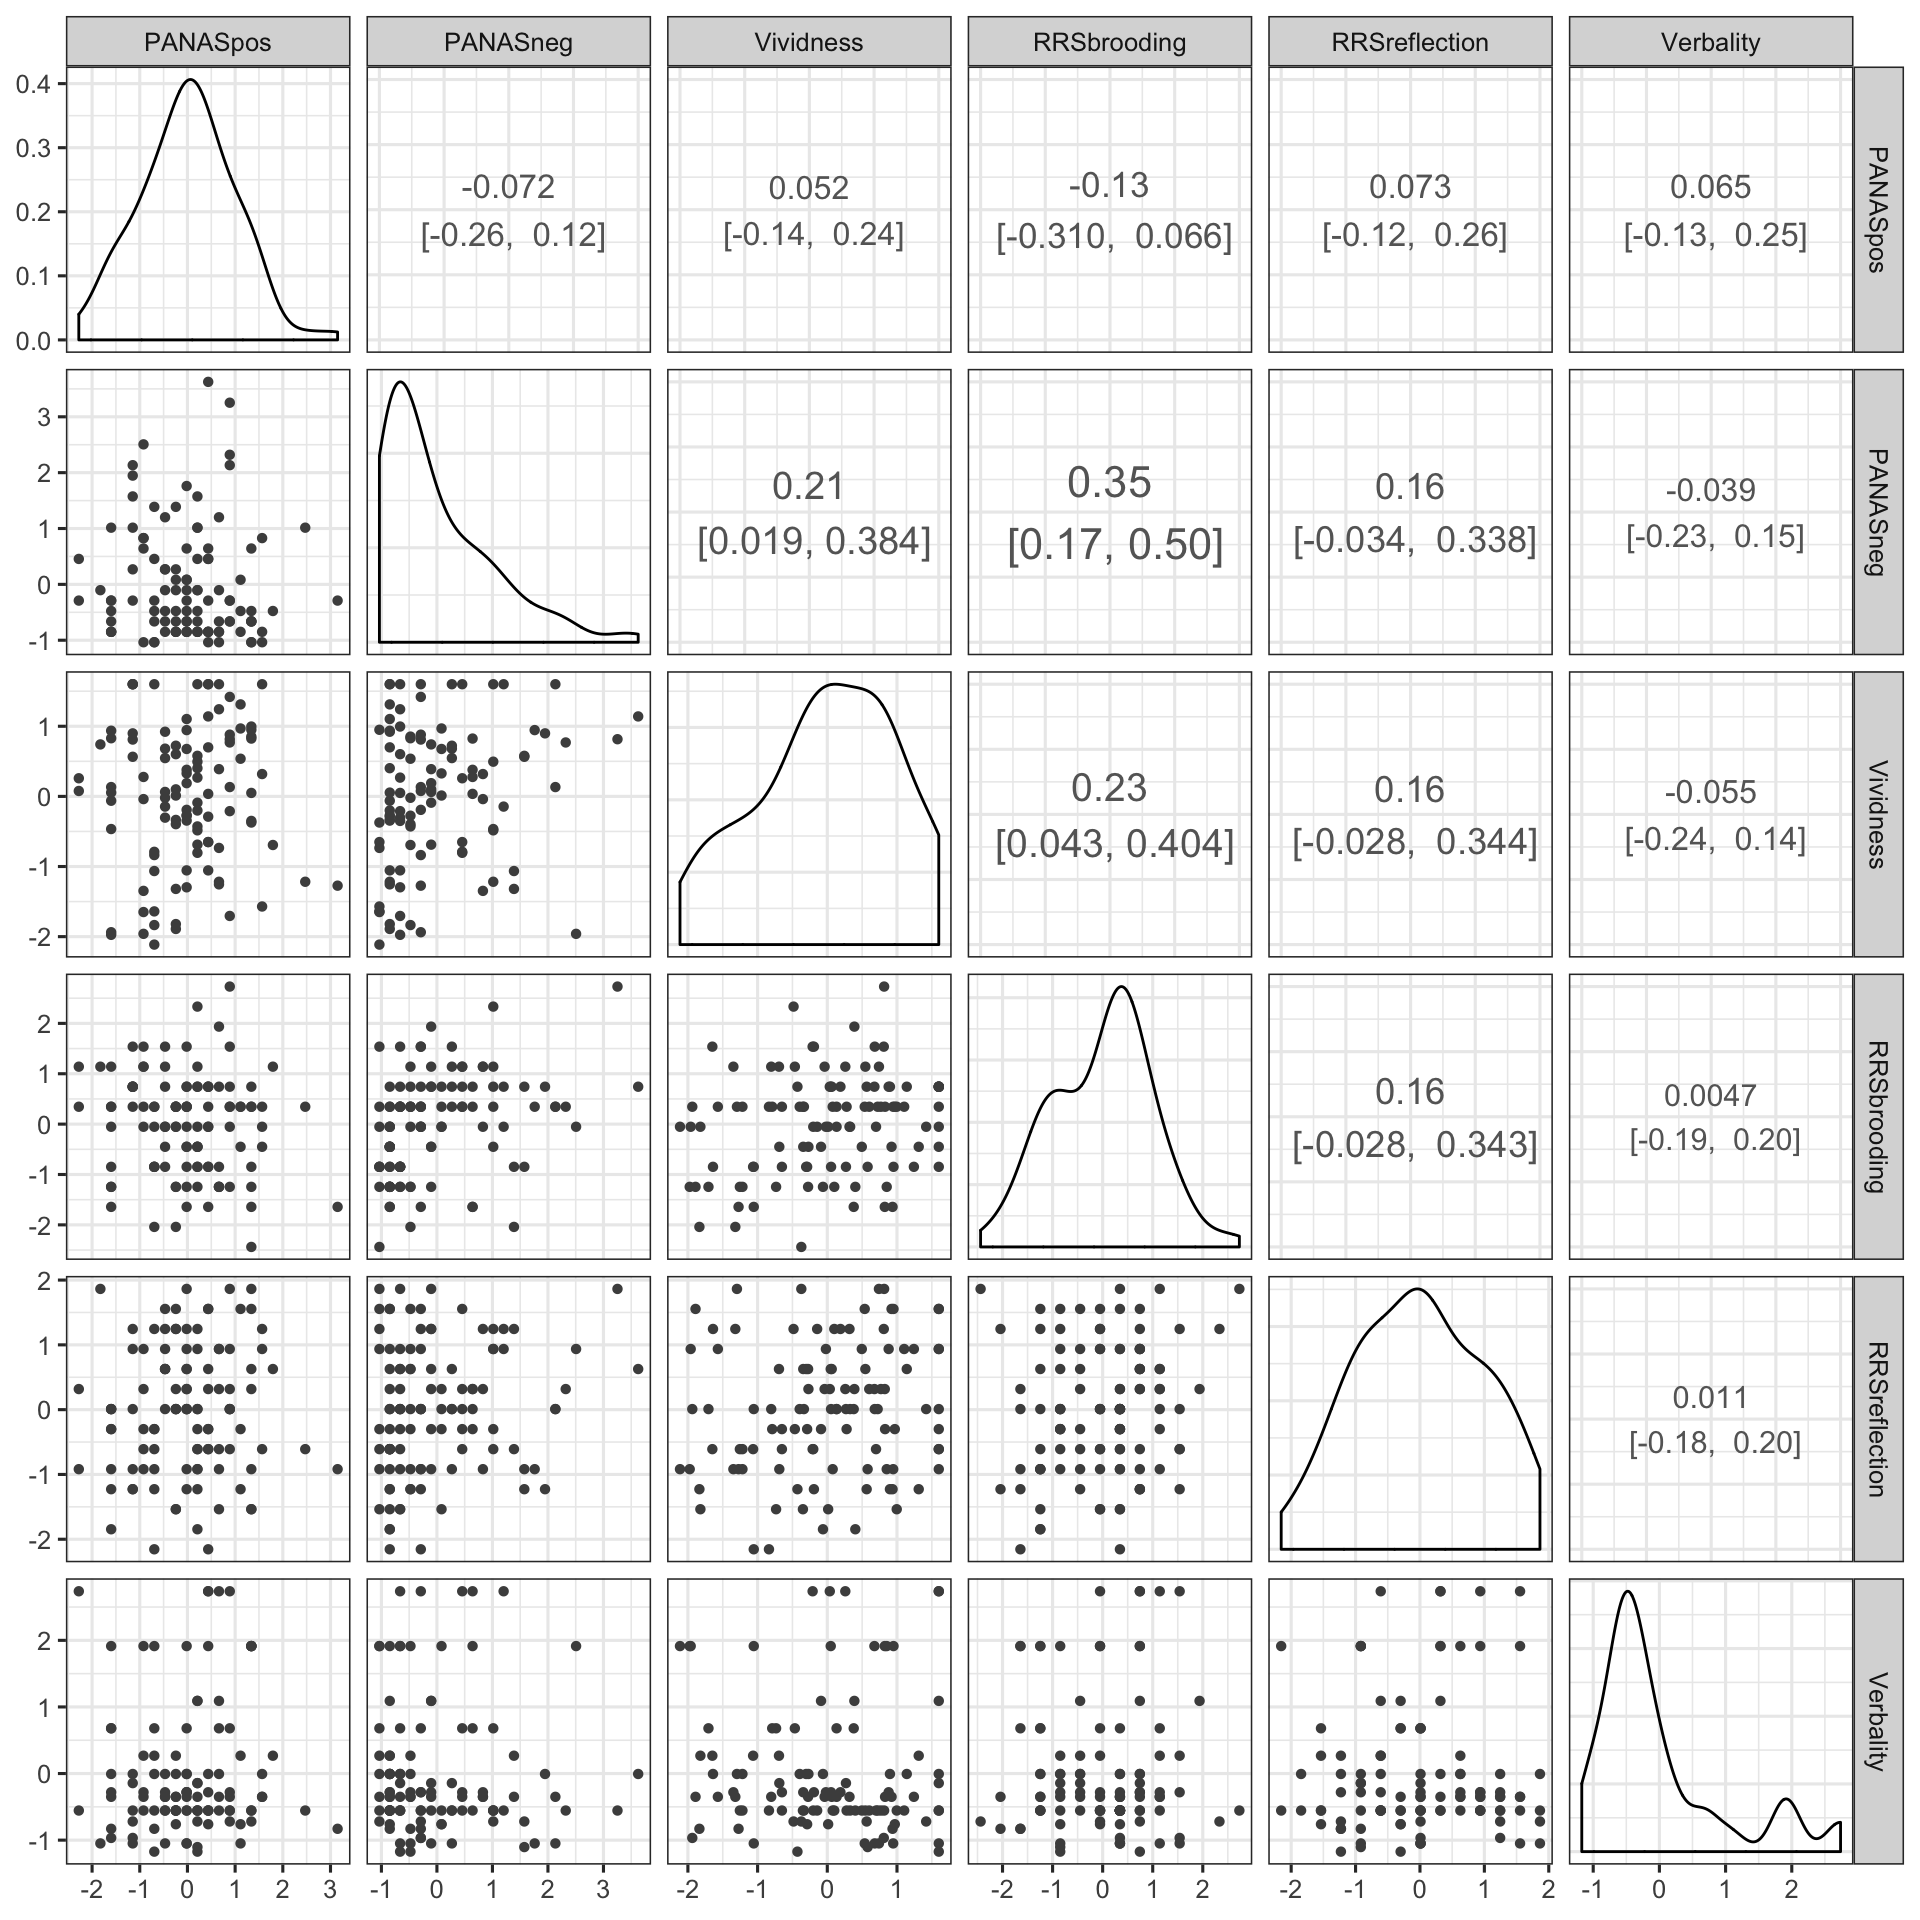
\includegraphics[width=1\linewidth]{06-chap6_files/figure-latex/correxp1-1} \caption{Diagonal: marginal distribution of each variable. Panels above the diagonal: Pearson's correlations between main continuous predictors, along with 95\% CIs. The absolute size of the correlation coefficient is represented by the size of the text (lower coefficients appear as smaller). Panels below the diagonal: scatterplot of each variables pair.}\label{fig:correxp1}
\end{figure}

\begin{lltable}
\small{
\begin{longtable}{lcccccc}\noalign{\getlongtablewidth\global\LTcapwidth=\longtablewidth}
\caption{\label{tab:sumstat}Descriptive statistics (mean and standard deviation) of each recorded variable, for the final sample of participants that were included in the study.}\\
\toprule
 & \multicolumn{3}{c}{Mouthing} & \multicolumn{3}{c}{Tapping} \\
\cmidrule(r){2-4} \cmidrule(r){5-7}
Variables & Baseline & Post-induction & Post-motor & Baseline & Post-induction & Post-motor\\
\midrule
RUM & 28.5 (26.49) & 54.66 (25.16) & 45.47 (27.25) & 20.96 (21.82) & 46.77 (25.74) & 43.54 (29.57)\\
Age & 20.3 (2.65) & - & - & 20.31 (2.53) & - & -\\
PANASneg & 15.65 (5.67) & - & - & 15.46 (5.08) & - & -\\
PANASpos & 30.91 (4.48) & - & - & 31.25 (4.4) & - & -\\
RRSbrooding & 12.2 (2.43) & - & - & 12.06 (2.62) & - & -\\
RRSreflection & 12.22 (3.22) & - & - & 11.71 (3.26) & - & -\\
Valence & 23.56 (22.4) & - & - & 37.53 (24.61) & - & -\\
Verbality & 1.67 (1.18) & - & - & 1.67 (1.26) & - & -\\
Vividness & 54.17 (28.94) & - & - & 59.78 (24.63) & - & -\\
\bottomrule
\end{longtable}
}
\end{lltable}

\hypertarget{rumination-induction-3}{%
\subsection{Rumination induction}\label{rumination-induction-3}}

To examine the efficiency of the induction procedure (i.e., the effect of \emph{Induction}) while controlling for the other variables (i.e., \emph{Vividness}, \emph{RRSbrooding}, \emph{RRSreflection}, \emph{PANASpos}, and \emph{PANASneg}), we then compared the parsimony of models containing main constant effects and a varying intercept for \emph{Participant}. Model comparison showed that the best model the model with the lowest WAIC) was the model including \emph{Induction}, \emph{PANASpos}, \emph{PANASneg}, \emph{RRSbooding}, and an interaction term between \emph{Induction} and \emph{Vividness} as predictors (see Table \ref{tab:compexp1}). Fit of the best model was moderate (\(R^2\) = 0.668, 95\% CrI {[}0.58, 0.736{]}).

\begin{lltable}
\begin{TableNotes}[para]
\textit{Note.} $pWAIC$ is the number of (effective) parameters in the model. $Int$ = Intercept, $Ind$ = Induction, $Viv$ = Vividness, $RRSbro$ = RRSbrooding, $RRSref$ = RRSreflection. All models include a varying intercept for Participant.
\end{TableNotes}
\small{
\begin{longtable}{lcccc}\noalign{\getlongtablewidth\global\LTcapwidth=\longtablewidth}
\caption{\label{tab:compexp1}Comparison of models, ordered by WAIC relative to the best model (i.e., the model with the lowest WAIC).}\\
\toprule
 & \multicolumn{1}{c}{$WAIC$} & \multicolumn{1}{c}{$pWAIC$} & \multicolumn{1}{c}{$\Delta_{WAIC}$} & \multicolumn{1}{c}{$Weight$}\\
\midrule
$Int+Ind+PANASpos+PANASneg+Ind:Viv+RRSbro$ & 1856.57 & 61.23 & 0.00 & 0.344\\
$Int+Ind+PANASpos+PANASneg+Ind:Viv+RRSbro+RRSref$ & 1856.64 & 61.38 & 0.07 & 0.332\\
$Int+Ind+PANASpos+PANASneg+Ind:Viv+RRSref$ & 1857.23 & 61.48 & 0.66 & 0.247\\
$Int+Ind+PANASneg+Ind:Viv$ & 1861.28 & 63.57 & 4.71 & 0.033\\
$Int+Ind+PANASpos+Ind:Viv$ & 1861.72 & 64.22 & 5.15 & 0.026\\
$Int+Ind+PANASneg$ & 1864.38 & 66.65 & 7.82 & 0.007\\
$Int+Ind+PANASpos$ & 1864.72 & 62.62 & 8.15 & 0.006\\
$Int+Ind+Ind:Viv$ & 1865.55 & 63.05 & 8.98 & 0.004\\
$Int+Ind$ & 1866.75 & 64.86 & 10.18 & 0.002\\
\bottomrule
\addlinespace
\insertTableNotes
\end{longtable}
}
\end{lltable}

Constant effect estimates for the best model are reported in Table \ref{tab:paramexp1}. Based on these values, it seems that \emph{Induction} (i.e., the effects of the rumination induction) increased \emph{RUM} scores by approximately 24.79 points on average (\(d_{av} =\) 1.037, 95\% CI {[}0.748, 1.325{]}). The main positive effect of \emph{PANASneg} and the main negative effects of \emph{PANASpos} indicate, respectively, that negative baseline mood was associated with higher levels of rumination while positive baseline mood was associated with lower levels of self-reported rumination.

\begin{table}[H]
\begin{center}
\begin{threeparttable}
\caption{\label{tab:paramexp1}Coefficient estimates, standard errors (SE), 95\% CrI (Lower, Upper), Rhat and Bayes factor (BF10) for the best model.}
\small{
\begin{tabular}{lcccccc}
\toprule
Term & \multicolumn{1}{c}{Estimate} & \multicolumn{1}{c}{SE} & \multicolumn{1}{c}{Lower} & \multicolumn{1}{c}{Upper} & \multicolumn{1}{c}{Rhat} & \multicolumn{1}{c}{BF10}\\
\midrule
Intercept & 37.787 & 1.928 & 33.985 & 41.575 & 1.00 & 1.293*10\textasciicircum{}16\\
Induction & 24.796 & 2.157 & 20.422 & 28.887 & 1.00 & -6.637*10\textasciicircum{}19\\
PANASpos & -6.612 & 1.928 & -10.358 & -2.887 & 1.00 & 48.97\\
PANASneg & 6.781 & 1.937 & 3.024 & 10.686 & 1.00 & 48.16\\
RRSbrooding & 2.689 & 1.988 & -1.545 & 6.391 & 1.00 & 0.467\\
Induction:Vividness & 4.072 & 2.140 & -0.255 & 8.362 & 1.00 & 1.256\\
\bottomrule
\addlinespace
\end{tabular}
}
\begin{tablenotes}[para]
\textit{Note.} As all predictors were centered to the mean for analysis, these coefficients approximate coefficients from simpler models.
\end{tablenotes}
\end{threeparttable}
\end{center}
\end{table}

Higher scores on \emph{Vividness} were associated with higher increase in self-reported rumination after induction, as revealed by the positive coefficient of the interaction term. This suggests that participants who recalled a more vivid negative memory tended to show a higher increase in rumination after the induction procedure than participants with a less vivid memory.

\hypertarget{articulatory-suppression-effects-on-induced-rumination}{%
\subsection{Articulatory suppression effects on induced rumination}\label{articulatory-suppression-effects-on-induced-rumination}}

We then examined the effect of the two motor tasks (articulatory suppression and finger-tapping) on \emph{RUM} while controlling for other variables (i.e., \emph{Vividness}, \emph{RRSbrooding}, \emph{RRSreflection}, \emph{Verbality}, \emph{PANASpos}, and \emph{PANASneg}). Given the group differences on \emph{RUM} score at baseline (i.e., after training), we also included this score as a control variable in our models, as the \emph{RUMb} variable. Based on our hypotheses, we expected that the model comparison would reveal a three-way interaction between \emph{Session}, \emph{Condition} and \emph{Verbality}. However, the best model identified by the WAIC model comparison did not include this interaction as a constant effect. Absolute fit of this model was moderate (\(R^2\) = 0.654, 95\% CrI {[}0.558, 0.724{]}).

\begin{lltable}
\begin{TableNotes}[para]
\textit{Note.} $K$ is the number of estimated parameters in the model. $Int$ = Intercept, $Cond$ = Condition, $RUMb$ = RUM baseline score, $Verb$ = Verbality, $RRSb$ = RRSbrooding, $RRSr$ = RRSreflection. All models include a constant intercept and a varying intercept for Participant.
\end{TableNotes}
\small{
\begin{longtable}{lcccc}\noalign{\getlongtablewidth\global\LTcapwidth=\longtablewidth}
\caption{\label{tab:compexp2}Comparison of models, ordered by WAIC relative to the best model (i.e., the model with the lowest WAIC).}\\
\toprule
 & \multicolumn{1}{c}{$WAIC$} & \multicolumn{1}{c}{$pWAIC$} & \multicolumn{1}{c}{$\Delta_{WAIC}$} & \multicolumn{1}{c}{$Weight$}\\
\midrule
$Session+Cond+Session:Cond+RUMb+PANASn+RRSb+RRSr$ & 1857.83 & 64.34 & 0.00 & 0.492\\
$Session+Cond+RUMb+PANASn+RRSb+RRSr$ & 1859.47 & 63.34 & 1.64 & 0.217\\
$Session+Cond+Session:Cond+Session:Cond:Verb+RUMb+PANASp+RRSb+RRSr$ & 1860.58 & 64.73 & 2.75 & 0.125\\
$Session+Cond+Session:Cond+Session:Cond:Verb+RUMb+PANASn+RRSb+RRSr$ & 1860.98 & 64.74 & 3.15 & 0.102\\
$Session+Cond+Session:Cond$ & 1863.85 & 69.13 & 6.01 & 0.024\\
$Session+Cond$ & 1863.97 & 68.60 & 6.14 & 0.023\\
$Session$ & 1865.88 & 68.99 & 8.05 & 0.009\\
$Session+Cond+Session:Cond:Verb$ & 1866.08 & 69.28 & 8.25 & 0.008\\
$Null\ model$ & 1878.41 & 67.31 & 20.58 & 0.000\\
\bottomrule
\addlinespace
\insertTableNotes
\end{longtable}
}
\end{lltable}

Parameter values of the best model for the second part of the experiment are reported in Table \ref{tab:paramexp2}. Based on these values, it seems that self-reported rumination decreased after both motor tasks (the coefficient for \emph{Session} is negative), but this decrease was substantially larger in the \emph{Mouthing} condition (\(d_{av} =\) -0.351, 95\% CI {[}-0.735, 0.034{]}) than in the \emph{Tapping} condition (\(d_{av} =\) -0.117, 95\% CI {[}-0.506, 0.273{]}), as can be read from the coefficient of the interaction term between \emph{Session} and \emph{Condition} (\emph{Est} = 4.975, \emph{SE} = 4.131, \emph{95\% CrI} {[}-2.771, 13.43{]}). However, the large uncertainty associated with this result (as expressed by the width of the confidence interval) warrants a careful interpretation of this result, that should be considered as suggestive evidence, rather than conclusive evidence.

However, the Bayesian framework provides tools that permit richer inference. First, we can compare the relative weight of the best model (the model with the lowest WAIC) with a similar model without the interaction term (the second model in Table \ref{tab:compexp2}). This reveals that the model including an interaction term between \emph{Session} and \emph{Condition} is 2.266519 more \emph{credible} than the model without the interaction term, which can be considered as weak but meaningful evidence (Burnham \& Anderson, \protect\hyperlink{ref-burnham_model_2002}{2002}).

Second, we can look at the BF for this particular parameter. As can be seen from Table \ref{tab:paramexp2}, the BF for the interaction term is equal to 1.19, which is evidence for neither the presence or the absence of effect. However, this BF is computed using the Savage-Dickey method\footnote{This method simply consists in taking the ratio of the posterior density at the point of interest divided by the prior density at that point (for a practical introduction, see Wagenmakers et al., \protect\hyperlink{ref-wagenmakers_bayesian_2010}{2010}).} and as such is extremely sensitive to the prior choice. Thus, other priors (for instance a prior that is more peaked on zero) would provide stronger evidence for the interaction effect.

\begin{table}[H]
\begin{center}
\begin{threeparttable}
\caption{\label{tab:paramexp2}Coefficient estimates, standard errors (SE), 95\% CrI (Lower, Upper), Rhat and Bayes factor (BF10) for the best model.}
\small{
\begin{tabular}{lcccccc}
\toprule
Term & \multicolumn{1}{c}{Estimate} & \multicolumn{1}{c}{SE} & \multicolumn{1}{c}{Lower} & \multicolumn{1}{c}{Upper} & \multicolumn{1}{c}{Rhat} & \multicolumn{1}{c}{BF10}\\
\midrule
Intercept & 47.554 & 2.000 & 43.712 & 51.590 & 1.000 & 5.169*10\textasciicircum{}16\\
Session & -5.901 & 2.110 & -10.120 & -1.814 & 1.000 & 10.32\\
Condition & -0.989 & 3.682 & -8.409 & 6.239 & 1.000 & 0.368\\
RUMbaseline & 12.854 & 2.287 & 8.718 & 17.372 & 1.001 & -3.695*10\textasciicircum{}17\\
RRSbrooding & 2.458 & 2.014 & -1.503 & 6.686 & 1.001 & 0.432\\
RRSreflection & -1.869 & 1.992 & -5.972 & 1.945 & 1.001 & 0.314\\
PANASneg & 0.517 & 2.239 & -3.930 & 4.890 & 1.001 & 0.227\\
Session:Condition & 4.975 & 4.131 & -2.771 & 13.430 & 1.000 & 0.837\\
\bottomrule
\addlinespace
\end{tabular}
}
\begin{tablenotes}[para]
\textit{Note.} As all predictors were centered to the mean for analysis, these coefficients approximate coefficients from simpler models.
\end{tablenotes}
\end{threeparttable}
\end{center}
\end{table}

The large variation between participants can be appreciated by computing the \emph{intra-class correlation} (ICC), expressed as \(\sigma_{intercept}^{2}/(\sigma_{intercept}^{2}+\sigma_{residuals}^{2})\). For the best model, the ICC is equal to 0.524 (95\% CrI {[}0.382, 0.662{]}), indicating that 52.4\% of the variance in the outcome that remains after accounting for the effect of the predictors, is attributable to systematic inter-individual differences.

Figure \ref{fig:plotexp1} shows the evolution of the mean \emph{RUM} scores all through the experiment according to each \emph{Session} (Baseline, Post-induction, Post-motor) and \emph{Condition} (Mouthing, Tapping). This figure reveals important inter-individual variability, in all conditions. After the rumination induction, \emph{RUM} score increased in both groups, and decreased after the motor task, with a stronger decrease in the \emph{Mouthing} condition.

\begin{figure}[H]
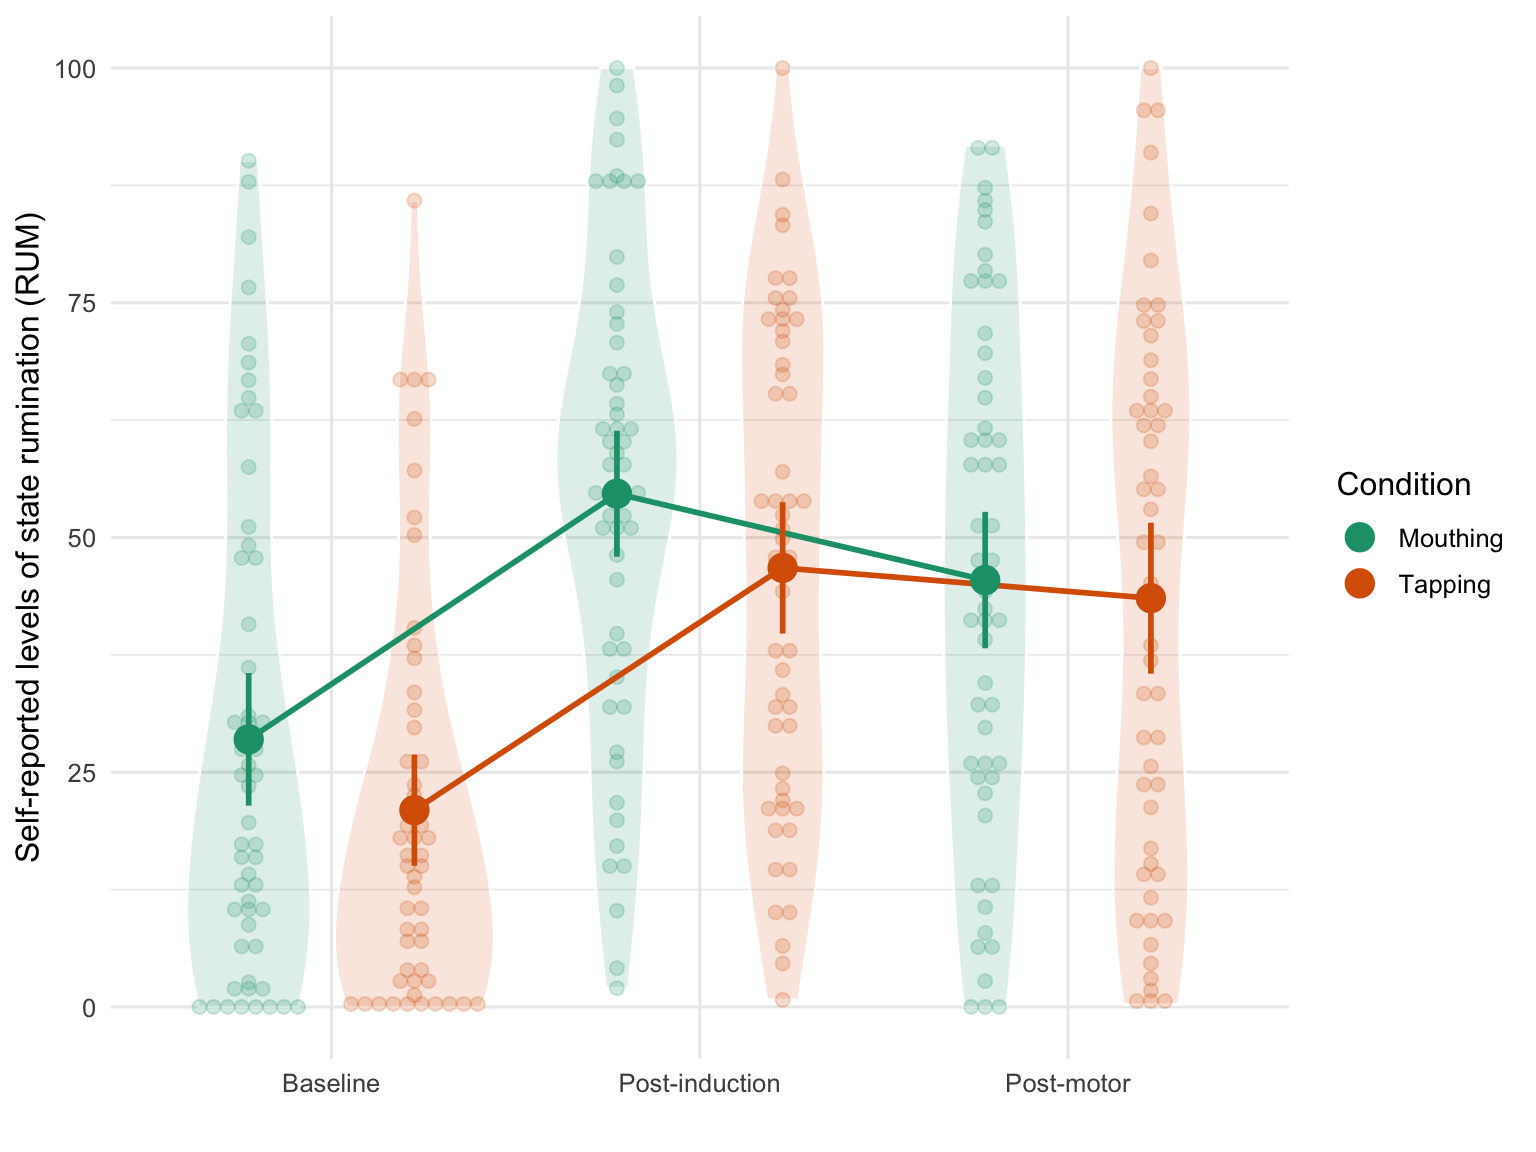
\includegraphics[width=1\linewidth]{06-chap6_files/figure-latex/plotexp1-1} \caption{Mean RUM score by Session and Condition, along with violin plots and individual data. Error bars represent 95\% CIs.}\label{fig:plotexp1}
\end{figure}

Figure \ref{fig:plotverbal} shows the effects of \emph{Verbality} on the relative change (i.e., after - before) in self-reported rumination after both motor activities (i.e., \emph{Mouthing} and \emph{Tapping}). As \emph{Verbality} was centered before analysis, its score cannot be interpreted in absolute terms. However, a high score on this index indicates more verbal than non-verbal (e.g., visual images, non-speech sounds) thoughts, whereas a low score indicates more non-verbal than verbal thoughts. Contrary to our predictions but consistent with the model comparison, this figure depicts a similar relationship between \emph{Verbality} and the change in \emph{RUM} score (between before and after the motor task), according to the Condition.

\begin{figure}[H]
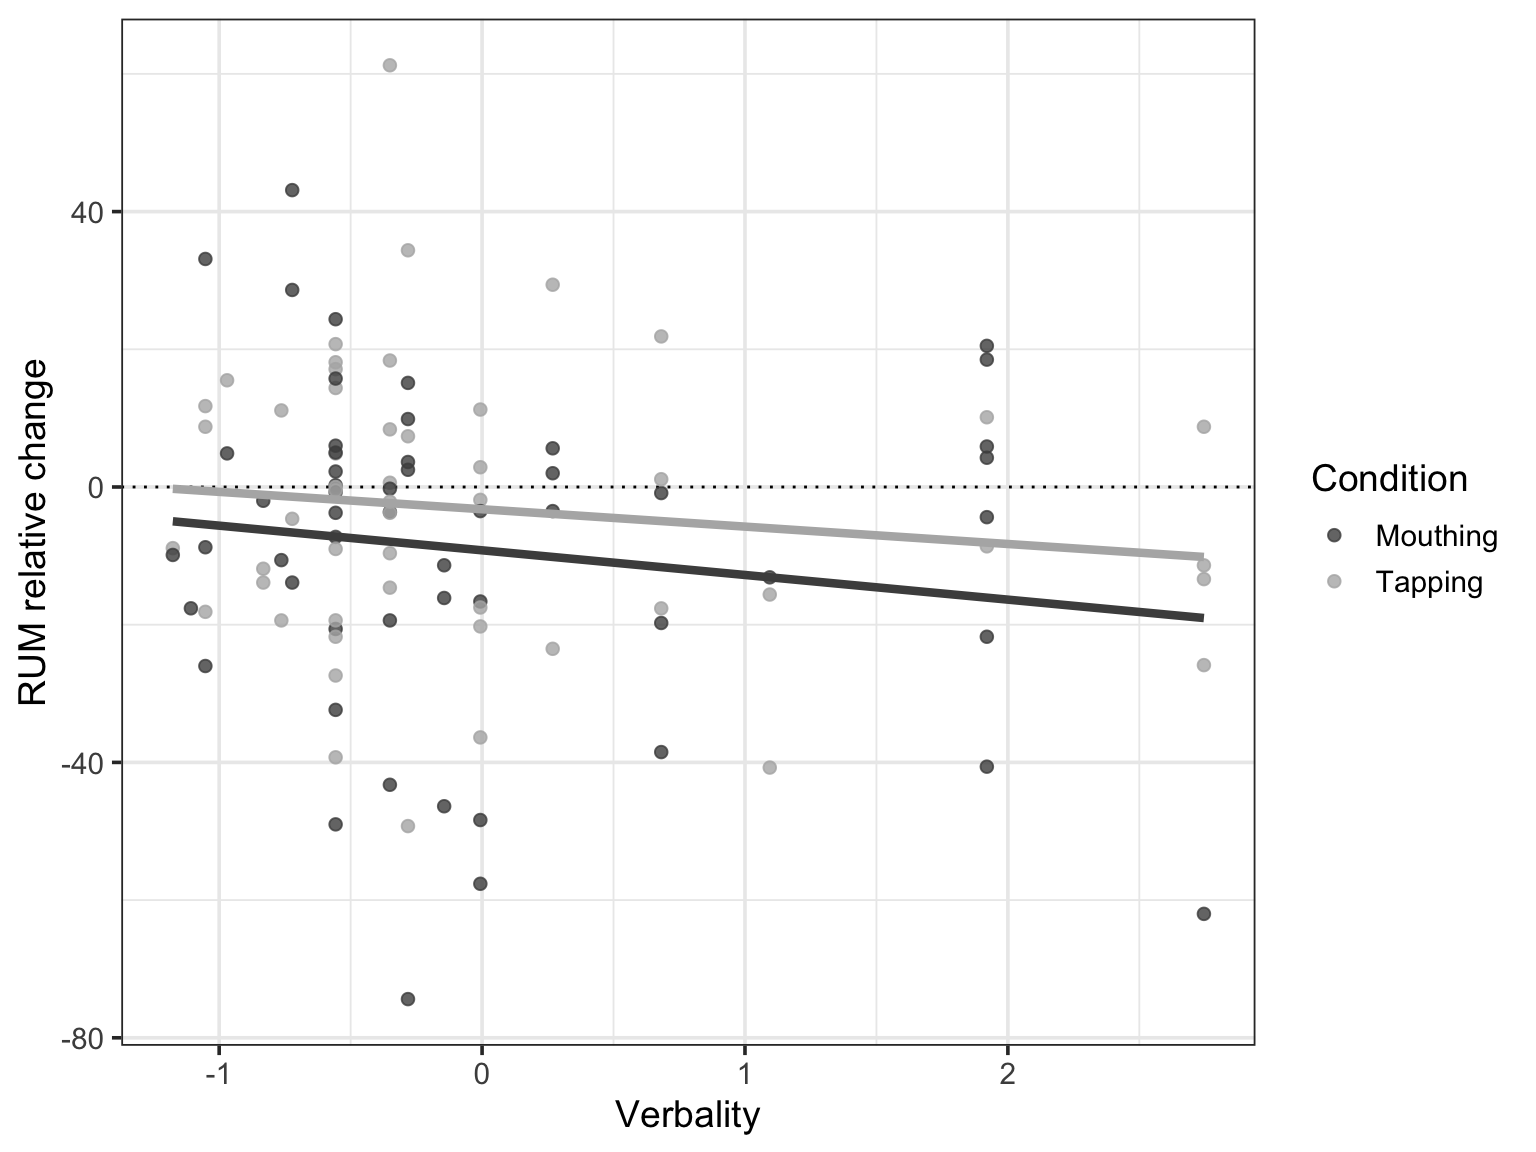
\includegraphics[width=1\linewidth]{06-chap6_files/figure-latex/plotverbal-1} \caption{Mean RUM relative change after motor activity, as a function of the degree of Verbality, in the mouthing (the green dots and regression line) and finger tapping (the orange dots and regression line) conditions.}\label{fig:plotverbal}
\end{figure}

\hypertarget{discussion-3}{%
\section{Discussion}\label{discussion-3}}

The purpose of the current study was to investigate the effects of articulatory suppression on induced verbal rumination. We predicted that if verbal rumination, which can be construed as a type of inner speech, does involve the mental simulation of overt speech production, its generation should be disrupted by articulatory suppression, but not by finger tapping. This prediction was not strictly corroborated by the data, as we observed a decrease of self-reported rumination after both types of motor activities (see Figure \ref{fig:plotexp1} and Table \ref{tab:compexp2}), with a somewhat stronger decrease in the Mouthing condition. In the following, we examine the validity of our methods and discuss interpretations of our results. Finally, we formulate how subsequent research should address this kind of question and suggest alternative ways to test the above mentioned hypothesis. We begin by discussing the results of the rumination induction procedure.

\hypertarget{rumination-induction-4}{%
\subsection{Rumination induction}\label{rumination-induction-4}}

It is noteworthy that 32.91\% of the total sample of participants who were recruited did not respond to this induction, and were therefore not included in the analyses. Moreover, as reported in Table \ref{tab:paramexp1}, it seems that the \emph{Vividness} of the memory chosen by the participant during the mood induction was moderating the effect of the rumination induction. In other words, the more vivid (i.e., the more \enquote{intense}) the memory, the more successful the rumination induction was. This highlights the fact that this aspect should be carefully controlled each time a mood induction is used in order to foster subsequent repetitive negative thinking.

Moreover, we observed a group difference of approximately 7.5 points in the average \emph{RUM} score at baseline. This difference might be explained by motor training, which took place before baseline measurement of state rumination. During this training, participants had to perform the motor task (either finger-tapping or mouthing) in front of a screen on which a white dot was moving randomly on a black screen, for 1 min. During the task, the experimenter stayed in the room (out of the participant's sight) to check that participants were performing the motor task adequately. Being an unusual and potentially embarrassing motor activity, mouthing might have been an higher source of stress for the participants, as compared to the more common activity of finger-tapping. This group difference in baseline state rumination subsisted after the induction, as the group difference after the induction was of approximately 8 points (see summary statistics in Table \ref{tab:sumstat}) and full dataset in the \protect\hyperlink{suppCh6}{supplementary materials}).

\hypertarget{articulatory-suppression-effects-1}{%
\subsection{Articulatory suppression effects}\label{articulatory-suppression-effects-1}}

In the following section, we discuss in more depth the results of the second part of the study, which aimed at comparing the effects of articulatory suppression and finger-tapping on self-reported rumination.

First, it is important to examine whether our failure to detect the predicted interaction could come from a lack of statistical power. We planned 128 participants in order to reach a power of .80 for a targeted effect size of \(\eta_{p}^{2}=.06\). As explained above, out of the 184 recruited participants, only 106 could be included in the study. With 106 participants, the a priori power for detecting an effect size of \(\eta_{p}^{2}=.06\) was approximately of .70, which is much higher than the median power in typical psychological studies.

Second, it is important to acknowledge that despite the absence of the predicted difference between the two conditions in their influence on the level of self-reported rumination (i.e., \emph{RUM}), both activities did lead, on average, to a decrease in self-reported rumination of approximately 6 points on the VAS (as indicated by the slope for \emph{Session} in Table \ref{tab:paramexp2}). This decrease might be interpreted in at least two ways. First, it might be explained by the simple exposition to the VAS and by compliance effects. When asked to rate their level of rumination again after five minutes of motor activity, some participants might be prompted to indicate a lower level of rumination than before the motor task. But compliance effects could similarly lead participants to consider the motor task as irritating, and therefore as prone to rumination increase. Some participants could therefore also be biased towards indicating a higher level of rumination after the motor task. Second, it might be considered that this decrease reflects a genuine decrease in rumination. In the following, we adopt the latter perspective and discuss explanations for the weak difference between the two conditions.

\hypertarget{effect-of-the-rumination-quality-verbality}{%
\subsubsection{Effect of the rumination quality (verbality)}\label{effect-of-the-rumination-quality-verbality}}

Our prediction was that rumination in verbal form would be more disrupted by mouthing than rumination in non-verbal form, while both kinds of rumination would not be disrupted (or similarly disrupted) by finger-tapping. In other words, we hypothesised a three-way interaction, between the effect of time (i.e., \emph{Session}), \emph{Condition}, and \emph{Verbality}. In the following, we discuss the absence of this interaction. Then, we focus on the weak difference between the two conditions (omitting \emph{Verbality}), and discuss some explanations for this weak difference.

First, the absence of the three-way interaction might come from a difficulty for the participants to have clear introspective access to the ruminative thoughts they experienced during the experiment. For instance, we know that introspective description of inner speech differs considerably, between people trained to regularly report on their episodes of inner speaking, and people without such training (e.g., Hurlburt et al., \protect\hyperlink{ref-Hurlburt2013}{2013}). Moreover, as the \emph{Verbality} questionnaire was presented at the end of the experiment, one cannot exclude that it was partly contaminated by recall, which, when done verbally, has been shown to artificially increase the subjective verbality index (Hurlburt, \protect\hyperlink{ref-Hurlburt2011}{2011}).

\hypertarget{difference-between-motor-conditions}{%
\subsubsection{Difference between motor conditions}\label{difference-between-motor-conditions}}

Leaving the self-reported quality of rumination aside, we now turn to a discussion of the weak difference between the two conditions. We think this result can be explained in at least two non-exclusive ways. First, we could argue that the decrease observed in both conditions was due to an unexpected effect of finger-tapping on rumination. Second, we could argue that the effect of the articulatory suppression was somehow weaker than expected. In the following, we provide arguments and explanations for each of these possibilities.

Steady finger-tapping is usually considered as a relevant control condition for evaluating articulatory suppression, since it specifically recruits the hand motor system and should not interfere with the oral motor system, while being comparable in terms of general attentional demands (e.g., Gruber, \protect\hyperlink{ref-gruber_effects_2001}{2001}; Logie \& Baddeley, \protect\hyperlink{ref-logie_cognitive_1987}{1987}). However, using more complex rhythmic patterns of finger-tapping, Saito (\protect\hyperlink{ref-saito_what_1994}{1994}) observed a fade-out of the phonological similarity effect in a verbal memory task with spoken recall, when subjects were asked to tap with either their right (dominant) or left hand, while the phonological similarity effect was conserved in the control condition (no tapping). The author concluded that a complex rhythmic tapping task can suppress the activity of the articulatory control process, by \emph{suppressing} the running of speech motor programs (Saito, \protect\hyperlink{ref-saito_what_1994}{1994}, p. 185). More specifically, he suggested that complex, non-automatised, rhythmic finger tapping could use speech motor programs, which are useful to control speech prosody, and therefore can deal with rhythmic activity. We further suggest that a novel complex rhythmic task might require silent verbalisation and, therefore, might itself be an articulatory suppression task. In line with these findings, another study showed that for right-handed subjects, tapping with a finger of the right hand is more effective at interfering with performance of a verbal memory task than is tapping with a finger of the left hand (Friedman, Polson, \& Dafoe, \protect\hyperlink{ref-friedman_dividing_1988}{1988}). Although Friedman et al.'s findings are difficult to interpret, because task priority was manipulated and this may have led to conflict resolution, which might have been dealt with differentially according to the hand involved, they do suggest that a finger tapping task is not always the best control for articulatory suppression. This might explain the decrease of self-reported rumination observed in our own study, after the finger-tapping, and suggests that we might observe different results by asking participants to tap with the finger of their non-dominant hand. We think it is important to note for future studies that our results, together with those of Saito (\protect\hyperlink{ref-saito_what_1994}{1994}) and Friedman et al. (\protect\hyperlink{ref-friedman_dividing_1988}{1988}), suggest that finger-tapping could in fact interfere with inner speech. In other words, finger-tapping, with the dominant hand, is probably not an appropriate control condition when studying articulatory suppression.

As suggested previously, an alternative way to explain the absence of differences between the two motor conditions is to suppose that the effects of the articulatory suppression were weaker than we expected. The rhythmic mouthing task might have become too automatised to disrupt inner speech programming. This idea finds some support in the results of Saito (\protect\hyperlink{ref-saito_when_1997}{1997}), who observed an effect of articulatory suppression on the phonological similarity effect in a memory task only when the articulatory suppression was \emph{intermittent} (i.e., \enquote{ah, ah, ah\ldots{}}) but no effect when participants had to utter a continuous \enquote{ah--}. This can be explained by considering that the intermittent articulatory suppression would impose a greater load on speech motor programming than the continuous articulatory suppression (Saito, \protect\hyperlink{ref-saito_when_1997}{1997}, p. 569). In a similar vein, Macken \& Jones (\protect\hyperlink{ref-macken_functional_1995}{1995}) found stronger effects of articulatory suppression when participants were asked to repeat a sequence of different letters than when they were asked to repeat a single letter. One way to examine this hypothesis with our own protocol would be to ask participants to make sequences of various mouth movements, rather than repeating a single movement.

In a broader perspective, relating to the original research question, we should mention two additional interpretations of our results. So far, we considered different ways to explain either how the finger-tapping task could interfere with rumination or how the articulatory suppression task might have failed to disrupt rumination. However, if we assume that our scales (especially the \emph{RUM} outcome response and the \emph{Verbality} scale) are reliable and that the articulatory suppression was efficient in its intended purpose, we are forced to admit that either i) rumination is not a type of inner speech that can be disrupted by peripheral muscle perturbation (i.e., it could be described as a more abstract form of inner speech) or that ii) inner speech, more broadly, does not depend on peripheral speech muscle activity. Although we think that these questions cannot be answered from our present results, we acknowledge that these two possibilities are compatible with our results.

In summary, the current research is one of the first behavioural studies exploring the association between verbal rumination and the speech motor system. While the observed data did not strictly corroborate our original hypotheses, we explored several explanations for the weak difference between articulatory suppression and the control task, and related our findings to previous works on the role of inner speech in verbal working memory. These results have important implications for future studies on articulatory suppression during inner speech or working memory tasks. More precisely, they highlight the need for further investigation of the most appropriate control task when studying the effects of articulatory suppression.

\hypertarget{acknowledgements-3}{%
\section{Acknowledgements}\label{acknowledgements-3}}

We thank David Meary for his technical support in programming the eye-tracking experiment, Elena Keracheva for her help during data collection as well as Rafael Laboissiere and Brice Beffara for their advice concerning data analysis.

A lot of useful packages have been used for the writing of this paper, among which the \texttt{papaja} and \texttt{knitr} packages for writing and formatting (Aust \& Barth, \protect\hyperlink{ref-R-papaja}{2018}; Xie, \protect\hyperlink{ref-R-knitr}{2018}), the \texttt{ggplot2}, \texttt{ggforce}, \texttt{GGally}, \texttt{DiagrammeR}, \texttt{patchwork}, \texttt{BEST}, and \texttt{plotly} packages for plotting (Iannone, \protect\hyperlink{ref-R-DiagrammeR}{2018}; Kruschke \& Meredith, \protect\hyperlink{ref-R-BEST}{2018}; Pedersen, \protect\hyperlink{ref-R-patchwork}{2017}, \protect\hyperlink{ref-R-ggforce}{2018}; Schloerke et al., \protect\hyperlink{ref-R-GGally}{2018}; Sievert et al., \protect\hyperlink{ref-R-plotly}{2017}; Wickham et al., \protect\hyperlink{ref-R-ggplot2}{2018}), the \texttt{sjstats} and \texttt{tidybayes} packages for data analysis (Kay, \protect\hyperlink{ref-R-tidybayes}{2018}; Lüdecke, \protect\hyperlink{ref-R-sjstats}{2018}), as well as the \texttt{tidyverse} and \texttt{glue} packages for code writing and formatting (Hester, \protect\hyperlink{ref-R-glue}{2017}; Wickham, \protect\hyperlink{ref-R-tidyverse}{2017}).

\hypertarget{funding-information}{%
\section{Funding information}\label{funding-information}}

This project was funded by the ANR project INNERSPEECH (grant number ANR-13-BSH2-0003-01). The first author of the manuscript is funded by a doctoral fellowship from Univ. Grenoble Alpes.

\hypertarget{suppCh6}{%
\section{Data Accessibility Statement}\label{suppCh6}}

Pre-registered protocol, preprint, data, as well as reproducible code and figures are available at: \href{http://osf.io/3bh67}{https://osf.io/3bh67/}.

\newpage

\begin{vplace}[1]

\begin{summary}{Summary of Chapter\getcurrentref{chapter}}

In this chapter, we set up a critical test of the \textit{motor simulation view} of inner speech (and rumination). Indeed, if the involvement of the speech motor system is \textit{necessary} during inner speech and rumination, then a disruption of the speech motor system should disrupt (or impair) the production of inner speech (and rumination). To examine this idea, we compared the effects of an articulatory suppression task to a finger-tapping task, following a rumination induction, on the levels of self-reported state rumination. Our results suggest a similar decrease in state rumination following both motor activities, suggesting that rumination would not be a form of inner speech that would crucially depend on the activity of the speech motor system (it does not mean that the speech motor system may never be involved in rumination, only that its involvement is not necessary). However, some important limitations make the interpretation of these results delicate. First, there were important differences between the two groups (i.e., articulatory suppression vs. finger-tapping groups) at baseline, possibly due do the rhythmic training proposed before baseline measurements. Second, the measure of state rumination consisted in one single non-validated scale (already used in Chapter 3) and may not be a reliable index of state rumination. Third, as in Chapter 3, there was no control group to the rumination induction and any effect following to the rumination induction may not be specifically attributable to the rumination induction. Fourth, there is some evidence suggesting that finger-tapping (with the dominant hand) may also perturbs speech motor planning and may therefore not be the best control condition to articulatory suppression. We try to overcome these limitations in the next and last empirical chapter.

\end{summary}

\end{vplace}

\hypertarget{chap7}{%
\chapter{Examining the involvement of the speech motor system during rumination: a dual-task investigation}\label{chap7}}

\initial{I}t has been suggested that verbal rumination may be considered as a form of inner speech and may therefore involve the speech motor system. This study explores whether the speech motor system is involved in verbal rumination by examining the effects of articulatory suppression (via gum-chewing) on two forms of induced repetitive thoughts (rumination and problem-solving), following the presentation of a stressor. We expected that (unconstrained) rumination would lead to sustained negative affects following a stressor whereas (unconstrained) problem-solving would lead to less detrimental effects on mood (in comparison to rumination). However, if motor processes are involved during rumination and problem-solving, articulatory suppression should dampen the differential effects of rumination and problem-solving on mood. At the time of the writing, data collection is still ongoing and the analyses presented in this chapter are therefore very preliminary. However, data collected so far suggest that articulatory suppression (gum-chewing) is indeed associated with a weaker difference in the effects of rumination versus problem-solving on state negative affects.\footnote{This experimental chapter is a working manuscript reformatted for the need of this thesis. Pre-registered protocol, preprint, data, as well as reproducible code and figures will be made available at: \url{https://osf.io/8ab2d/}.}

\hypertarget{introduction-4}{%
\section{Introduction}\label{introduction-4}}

The ability to talk to oneself silently is a core foundational ability that supports many higher cognitive functions such as remembering, planning, task-switching or problem-solving (for review, see Alderson-Day \& Fernyhough, \protect\hyperlink{ref-alderson-day_inner_2015}{2015}; Perrone-Bertolotti et al., \protect\hyperlink{ref-Perrone-Bertolotti2014}{2014}). Although inner speech supports many cognitive abilities, its dysfunctions are similarly numerous and diverse. For instance, auditory verbal hallucinations (i.e., intrusive and agency-less inner voices) or obsessional thoughts can be considered as occurrences of dysfunctional inner speech (Perrone-Bertolotti et al., \protect\hyperlink{ref-Perrone-Bertolotti2014}{2014}). In the present article, we focus on rumination, a form of repetitive negative thinking (Ehring \& Watkins, \protect\hyperlink{ref-ehring_repetitive_2008}{2008}) than can be broadly defined as unconstructive repetitive thinking about past events and current mood states (Martin \& Tesser, \protect\hyperlink{ref-Martin}{1996}).

Rumination has been consistently related to increased risks of onset and maintenance of depressive episodes (for review, see Ehring \& Watkins, \protect\hyperlink{ref-ehring_repetitive_2008}{2008}; Nolen-Hoeksema et al., \protect\hyperlink{ref-Nolen-Hoeksema2008}{2008}) and has been suggested to contribute in exacerbating current depression (e.g., Raedt \& Koster, \protect\hyperlink{ref-Raedt2010}{2010}). A particularly maladaptive and harmful form of rumination is brooding, defined as self-critical pondering on one's current or past mood states and unachieved goals (Treynor et al., \protect\hyperlink{ref-treynor_rumination_2003}{2003}). Brooding has been shown to uniquely contribute to the maladaptive consequences of self-focused repetitive thinking. Experimental studies have shown that induced rumination, in comparison to distraction or problem-solving, worsens (i.e., lengthens and/or intensifies) negative mood (e.g., Huffziger \& Kuehner, \protect\hyperlink{ref-Huffziger2009}{2009}; Philippot \& Brutoux, \protect\hyperlink{ref-Philippot2008}{2008}), impairs cognitive processes (e.g., Philippot \& Brutoux, \protect\hyperlink{ref-Philippot2008}{2008}; Whitmer \& Gotlib, \protect\hyperlink{ref-whitmer_switching_2012}{2012}) and increases the retrieval of overgeneral and negative autobiographic memories (e.g., Lyubomirsky et al., \protect\hyperlink{ref-Lyubomirsky1998}{1998}; Watkins \& Teasdale, \protect\hyperlink{ref-watkins_rumination_2001}{2001}).

Overall, rumination is known to be a predominantly verbal process (Ehring \& Watkins, \protect\hyperlink{ref-ehring_repetitive_2008}{2008}; Goldwin \& Behar, \protect\hyperlink{ref-goldwin_concreteness_2012}{2012}; Goldwin et al., \protect\hyperlink{ref-goldwin_concreteness_2013}{2013}; McLaughlin et al., \protect\hyperlink{ref-mclaughlin_effects_2007}{2007}) and has been proposed to be considered as such as a dysfunctional form of inner speech (e.g., Perrone-Bertolotti et al., \protect\hyperlink{ref-Perrone-Bertolotti2014}{2014}). On the other hand, research on the psychophysiology of inner speech revealed that the neural processes involved in overt speech and inner speech tend to be very similar. Indeed, both forms of speech involve a landscape of inferior frontal areas, motor and auditory areas (for an overview, see Lœvenbruck et al., \protect\hyperlink{ref-loevenbruck_cognitive_2018}{2018}). This is coherent with the idea that some forms of inner speech could be considered as a kind of simulation of overt speech (e.g., Postma \& Noordanus, \protect\hyperlink{ref-postma_production_1996}{1996}; Jeannerod, \protect\hyperlink{ref-jeannerod_motor_2006}{2006}), in the same way as imagined actions can be considered as the result of a simulation of the corresponding overt action (e.g., walking and imagined walking, Decety, Jeannerod, \& Prablanc, \protect\hyperlink{ref-decety_timing_1989}{1989}). In other words, the motor simulation hypothesis suggests that the speech motor system should be involved as well during inner speech production.

Accordingly, in the same way motor imagery is usually accompanied by peripheral muscular activation (for review, see Guillot et al., \protect\hyperlink{ref-guillot_electromyographic_2010}{2010}), inner speech production should also be accompanied by peripheral muscular activation in the speech muscles. This hypothesis has been corroborated by many studies showing peripheral muscular activation during inner speech production (e.g., Livesay et al., \protect\hyperlink{ref-livesay_covert_1996}{1996}; Locke, \protect\hyperlink{ref-locke_subvocal_1970-1}{1970}; Locke \& Fehr, \protect\hyperlink{ref-locke_subvocal_1970}{1970}; McGuigan \& Dollins, \protect\hyperlink{ref-mcguigan_patterns_1989}{1989}; McGuigan \& Winstead, \protect\hyperlink{ref-mcguigan_discriminative_1974}{1974}; Sokolov, \protect\hyperlink{ref-sokolov_inner_1972}{1972}), during auditory verbal hallucinations in patients with schizophrenia (Rapin et al., \protect\hyperlink{ref-rapin_emg_2013}{2013}\protect\hyperlink{ref-rapin_emg_2013}{a}) and during induced rumination (Nalborczyk et al., \protect\hyperlink{ref-nalborczyk_orofacial_2017}{2017}). Some authors also recently demonstrated that it was possible to decode inner speech content based on surface electromyography signals (Kapur et al., \protect\hyperlink{ref-kapur_alterego_2018}{2018}), although other teams failed to obtain such results (e.g., Meltzner et al., \protect\hyperlink{ref-meltzner_speech_2008}{2008}).

The corollary hypothesis might be drawn, according to which the production of inner speech (and rumination) should be disrupted by a disruption of the speech motor system. This idea is supported by a large number of working memory studies using articulatory suppression to disrupt the subvocal rehearsal component of working memory, leading to impaired recall performance (e.g., Baddeley et al., \protect\hyperlink{ref-baddeley_exploring_1984}{1984}; Larsen \& Baddeley, \protect\hyperlink{ref-larsen_disruption_2003}{2003}). Although articulatory suppression usually refers to the overt and vocalised repetition of speech sounds (e.g., repeating a syllable or a word out loud), several studies have shown that concurrent subvocalisation or mechanical perturbation of the speech motor system (e.g., unvoiced or mouthed speech) was also interfering with speech planning (e.g., Reisberg et al., \protect\hyperlink{ref-reisberg_enacted_1989}{1989}; Smith et al., \protect\hyperlink{ref-smith_role_1995}{1995}). Interestingly, the effects of this motor interference are usually described as increasingly efficient depending on the degree of \enquote{enactment}, ranging from silent mouthing to vocalised utterance (Reisberg et al., \protect\hyperlink{ref-reisberg_enacted_1989}{1989}).

The effects of articulatory suppression on inner speech production are also known to depend on other factors such as the complexity and the novelty of the inner speech content (Sokolov, \protect\hyperlink{ref-sokolov_inner_1972}{1972}). Similarly, the effects of articulatory suppression seem to vary according to the degree to which inner speech production has been automatised (e.g., rehearsing a poem learned by heart vs.~rehearsing a just heard phone number). Therefore, inner speech might be more or less affected by mechanical constraints, depending on the type of inner speech to be produced. In other words, inner speech might vary in form along several dimensions, such as \enquote{enactment} (i.e., the degree of implication of the speech motor system) or \enquote{abbreviatedness} (i.e., the abstractness vs.~concreteness of inner speech). These different dimensions and varieties of inner speech have been thoroughly studied by experience sampling methods and questionnaires (e.g., Hurlburt, \protect\hyperlink{ref-Hurlburt2011}{2011}; Hurlburt et al., \protect\hyperlink{ref-Hurlburt2013}{2013}; McCarthy-Jones \& Fernyhough, \protect\hyperlink{ref-McCarthy-Jones2011}{2011}) but also more recently using neuroimagery (Grandchamp et al., \protect\hyperlink{ref-grandchamp_neurocognitive_2019}{2019}). Therefore, a central question of the present article is to elucidate whether rumination is a form of inner speech that is affected by articulatory suppression.

It has been highlighted that \emph{earworms} (i.e., \enquote{involuntary musical imagery}) might share some similarities with repetitive negative thoughts such as obsessional thoughts (see review in Beaman \& Williams, \protect\hyperlink{ref-Beaman2010}{2010}). In a recent study, these authors have shown that chewing a gum induced a reduction in the number of self-reported earworms episodes, in comparison to a resting condition (Beaman, Powell, \& Rapley, \protect\hyperlink{ref-Beaman2015}{2015}). However, these results should be interpreted cautiously, as the gum-chewing condition was compared to a resting (passive) condition and not to an active control condition (e.g., finger-tapping) in Experiment 1 and Experiment 2. The results of the third experiment reported in Beaman et al. (\protect\hyperlink{ref-Beaman2015}{2015}), in which gum-chewing was compared to finger-tapping, suggest that gum-chewing might indeed be more efficient than finger-tapping in reducing the number of self-reported earworms episodes. However, it should be noted that these results contradict several previous results (e.g., Kozlov, Hughes, \& Jones, \protect\hyperlink{ref-kozlov_gummed-up_2012}{2012}) and should therefore be interpreted as suggestive.

To the best of our knowledge, only one study investigated the effects of a perturbation of the speech motor system on verbal repetitive negative thinking (Rapee, \protect\hyperlink{ref-rapee_utilisation_1993}{1993}). This study revealed a \enquote{marginally significant} decrease in worry-related thoughts following an articulatory suppression. In the same vein, we recently carried out a study in which we compared the effects of an articulatory suppression (silent mouthing) to the effects of finger-tapping following a rumination induction (Nalborczyk et al., \protect\hyperlink{ref-nalborczyk_articulatory_2018}{2018}). The results of this study revealed, as in Rapee (\protect\hyperlink{ref-rapee_utilisation_1993}{1993}), a marginally superior effect of articulatory suppression (compared to finger-tapping) in reducing self-reported state rumination. However, it was not clear whether this effect was due to articulatory suppression per se or to extraneous factors such as baseline differences (see discussion in Nalborczyk et al., \protect\hyperlink{ref-nalborczyk_articulatory_2018}{2018}).

In the present study, we aimed to investigate whether rumination involves articulatory features by interfering with the activity of the speech motor system during rumination. To this end, we compared the effects of an articulatory suppression (gum-chewing) to a control motor activity (finger-tapping), following either an induction of (verbal) rumination or an induction of (verbal) problem-solving. We expected to find less self-reported state rumination following a period of articulatory suppression than following a period of finger-tapping. Moreover, because both rumination and problem-solving are expected to be (at least partially) blocked by articulatory suppression, we expected articulatory suppression to reduce the detrimental effects of rumination on mood (in comparison to finger-tapping), whereas we expected articulatory suppression to reduce the beneficial (or less detrimental, in comparison to rumination) effects of problem-solving on mood (in comparison to finger-tapping).

\hypertarget{methods-4}{%
\section{Methods}\label{methods-4}}

In the \emph{Methods} and \emph{Data analysis} sections, we report how we determined our sample size, all data exclusions, all manipulations, and all measures in the study (Simmons et al., \protect\hyperlink{ref-simmons_21_2012}{2012}). A pre-registered version of our protocol can be found online: \url{https://osf.io/8ab2d/}.

\hypertarget{participants-3}{%
\subsection{Participants}\label{participants-3}}

We used the \emph{Sequential Bayes Factor} procedure as introduced in Schönbrodt et al. (\protect\hyperlink{ref-schonbrodt_sequential_2017}{2017}) to determine our sample size. We defined a statistical threshold as \(BF_{10} = 10\) and \(BF_{10} = \dfrac{1}{10}\) (i.e., \(BF_{01} = 10\)) on the effect of interest. More precisely, we were interested in the difference in self-reported state rumination after the period of motor activity between the two rumination groups. In order to prevent potential experimenter and demand biases during sequential testing, the experimenter was blind to Bayes factors computed on previous participants (Beffara, Bret, \& Nalborczyk, \protect\hyperlink{ref-beffara_fully_2019}{2019}). All statistical analyses have been automated and a single instruction was returned to the experimenter (i.e., \enquote{keep recruiting participants} or \enquote{stop the recruitment}). We fixed the minimum sample size to 100 participants (i.e., around 25 participants per group) to avoid early terminations of the sequential procedure and the maximum sample size to four weeks of experiment, including in total 255 potential time slots.

At the time of the writing, we were not able to conduct this procedure until its end. We currently have data for 42 participants. These participants were all female Dutch-speaking right-handed undergraduate students in Psychology at Ghent University (Mean age = 21.26, SD = 2.28). They were recruited via an online platform and were given 10\euro~in exchange for their participation. Each participant provided consent to participate and the present study was approved by the local ethical committee of the Psychology department at Ghent University.

\hypertarget{material-4}{%
\subsection{Material}\label{material-4}}

\hypertarget{trait-questionaire-measures}{%
\subsubsection{Trait questionaire measures}\label{trait-questionaire-measures}}

Trait rumination was assessed using the Dutch version of the 10-item revised Ruminative Response Scale (Raes, Hermans, \& Eelen, \protect\hyperlink{ref-raes_kort_2003}{2003}; Treynor et al., \protect\hyperlink{ref-treynor_rumination_2003}{2003}). This questionnaire comprises two subscales, evaluating either the \emph{Reflection} or the \emph{Brooding} component of rumination, where the latter refers to a less adaptive form of rumination (Treynor et al., \protect\hyperlink{ref-treynor_rumination_2003}{2003}). To assess the presence and severity of depressive symptoms, we administered the Dutch version of the 21-item Beck Depression Inventory (BDI-II-NL, Beck, Steer, \& Brown, \protect\hyperlink{ref-beck_manual_1996}{1996}; Van der Does, \protect\hyperlink{ref-van_der_does_nederlandse_2002}{2002}).

\hypertarget{state-questionaire-measures}{%
\subsubsection{State questionaire measures}\label{state-questionaire-measures}}

State rumination was assessed during the experiment via the Dutch version of the Brief State Rumination Inventory (BSRI, Marchetti et al., \protect\hyperlink{ref-marchetti_brief_2018}{2018}). This questionnaire comprises eight items measuring the extent to which participants are ruminating at the moment. These items were presented as visual analogue scales (VASs) subsequently recoded between 0 and 100. The BSRI total score is computed as the sum of these eight items and the BSRI has been shown to have good psychometric properties (Marchetti et al., \protect\hyperlink{ref-marchetti_brief_2018}{2018}). Positive and negative affects were monitored throughout the experiment using the Dutch version of the Positive and Negative Affect Schedule (PANAS, Engelen, Peuter, Victoir, Diest, \& Van den Bergh, \protect\hyperlink{ref-engelen_verdere_2006}{2006}; Watson et al., \protect\hyperlink{ref-watson_development_1988}{1988}).

\hypertarget{thinking-style-induction}{%
\subsubsection{Thinking-style induction}\label{thinking-style-induction}}

The thinking-style induction was adapted from Grol et al. (\protect\hyperlink{ref-grol_effects_2015}{2015}) and consisted in two parts. First, participants were asked to vividly imagine a car accident scenario from a first-person perspective (as if they were driving the car). They were given between 1min (minimum allocated time) and 5min (maximum allocated time) to imagine this situation. Second, participants were asked to think about this hypothetical situation and its consequences in either a ruminative manner or a problem-solving manner. To this end, a series a six prompts were presented successively on the screen (specific prompts can be found in the \protect\hyperlink{supp}{supplementary materials}). Each prompt was presented for a maximum duration of 2min and the participant was invited to type her thoughts in reaction to this prompt below the prompt. Participants were asked to type their thoughts as they came, without focusing too much on the grammatical correctness of the sentences they were typing.

\hypertarget{articulatory-suppression}{%
\subsubsection{Articulatory suppression}\label{articulatory-suppression}}

In the articulatory suppression condition, participants were asked to open an opaque box (disposed aside from the computer screen) in which they found chewing gums\footnote{These gums were chosen to be as neutral and usual as possible. More precisely, we used sugar-free and allergenic-free mint-flavoured gums.}. They were then asked to chew the gum in a \enquote{sustained but natural way} (in order to avoid too much interruption) during the next 5 minutes. In the finger-tapping condition, participants were asked to tap with the index of their non-dominant (i.e., left) arm at a \enquote{sustained but natural} pace for the next 5 minutes. In both conditions, participants were also asked to \enquote{continue to think about the car-accident situation and the following prompts}.

\hypertarget{procedure-4}{%
\subsection{Procedure}\label{procedure-4}}

Upon arriving at the laboratory, participants were asked whether they had recently been involved in a traffic accident. No participant was excluded on this basis. Participants then completed the BDI-II-NL questionnaire. No participant was excluded on the basis of a BDI-II-NL score greater than 29. Afterwards, participants were given a brief verbal overview of the experiment by the experimenter, before the experimenter definitely leaves the room. The participant then started the experiment on a computer. The experiment was programmed with the OpenSesame software program (Mathôt et al., \protect\hyperlink{ref-mathot_opensesame_2012}{2012}).

After filling-in the consent form, participants watched a series of short (around 30s each) neutral video clips for a total duration of 5mn in order to neutralise pre-existing mood differences between participants (Marchetti et al., \protect\hyperlink{ref-marchetti_brief_2018}{2018}; Samson, Kreibig, Soderstrom, Wade, \& Gross, \protect\hyperlink{ref-samson_eliciting_2015}{2015}). Then, participants filled-in baseline measurements of state rumination (BSRI) and state affects (PANAS). Afterwards, participants went through either a rumination or a problem-solving thinking induction, as described previously. Following this induction, participants filled-in again the BSRI questionnaire to check whether the rumination induction was successful in inducing rumination. Participants in each group were then randomly allocated to either a 5-min articulatory suppression condition (gum-chewing) or a 5-min finger-tapping condition, resulting in four groups of participants. Following the motor activity, participants filled-in again both the BSRI and the PANAS questionnaires. Then, participants filled-in the RRS questionnaire to assess their propensity to ruminate in daily life.

At the end of the experiment, all participants went through a positive mood induction (remembering and reliving a positive memory) to attenuate the effects of the stress induction. Finally, participants were fully debriefed about the goals of the study. The entire experiment was video-monitored using a Sony HANDYCAM video camera to check whether the participants effectively completed the task. In addition, the experimenter was able to monitor the participant's performance during the experiment through a one-way mirror (located behind the participant). This procedure is summarised in Figure \ref{fig:diagram}.

\begin{figure}[H]

{\centering 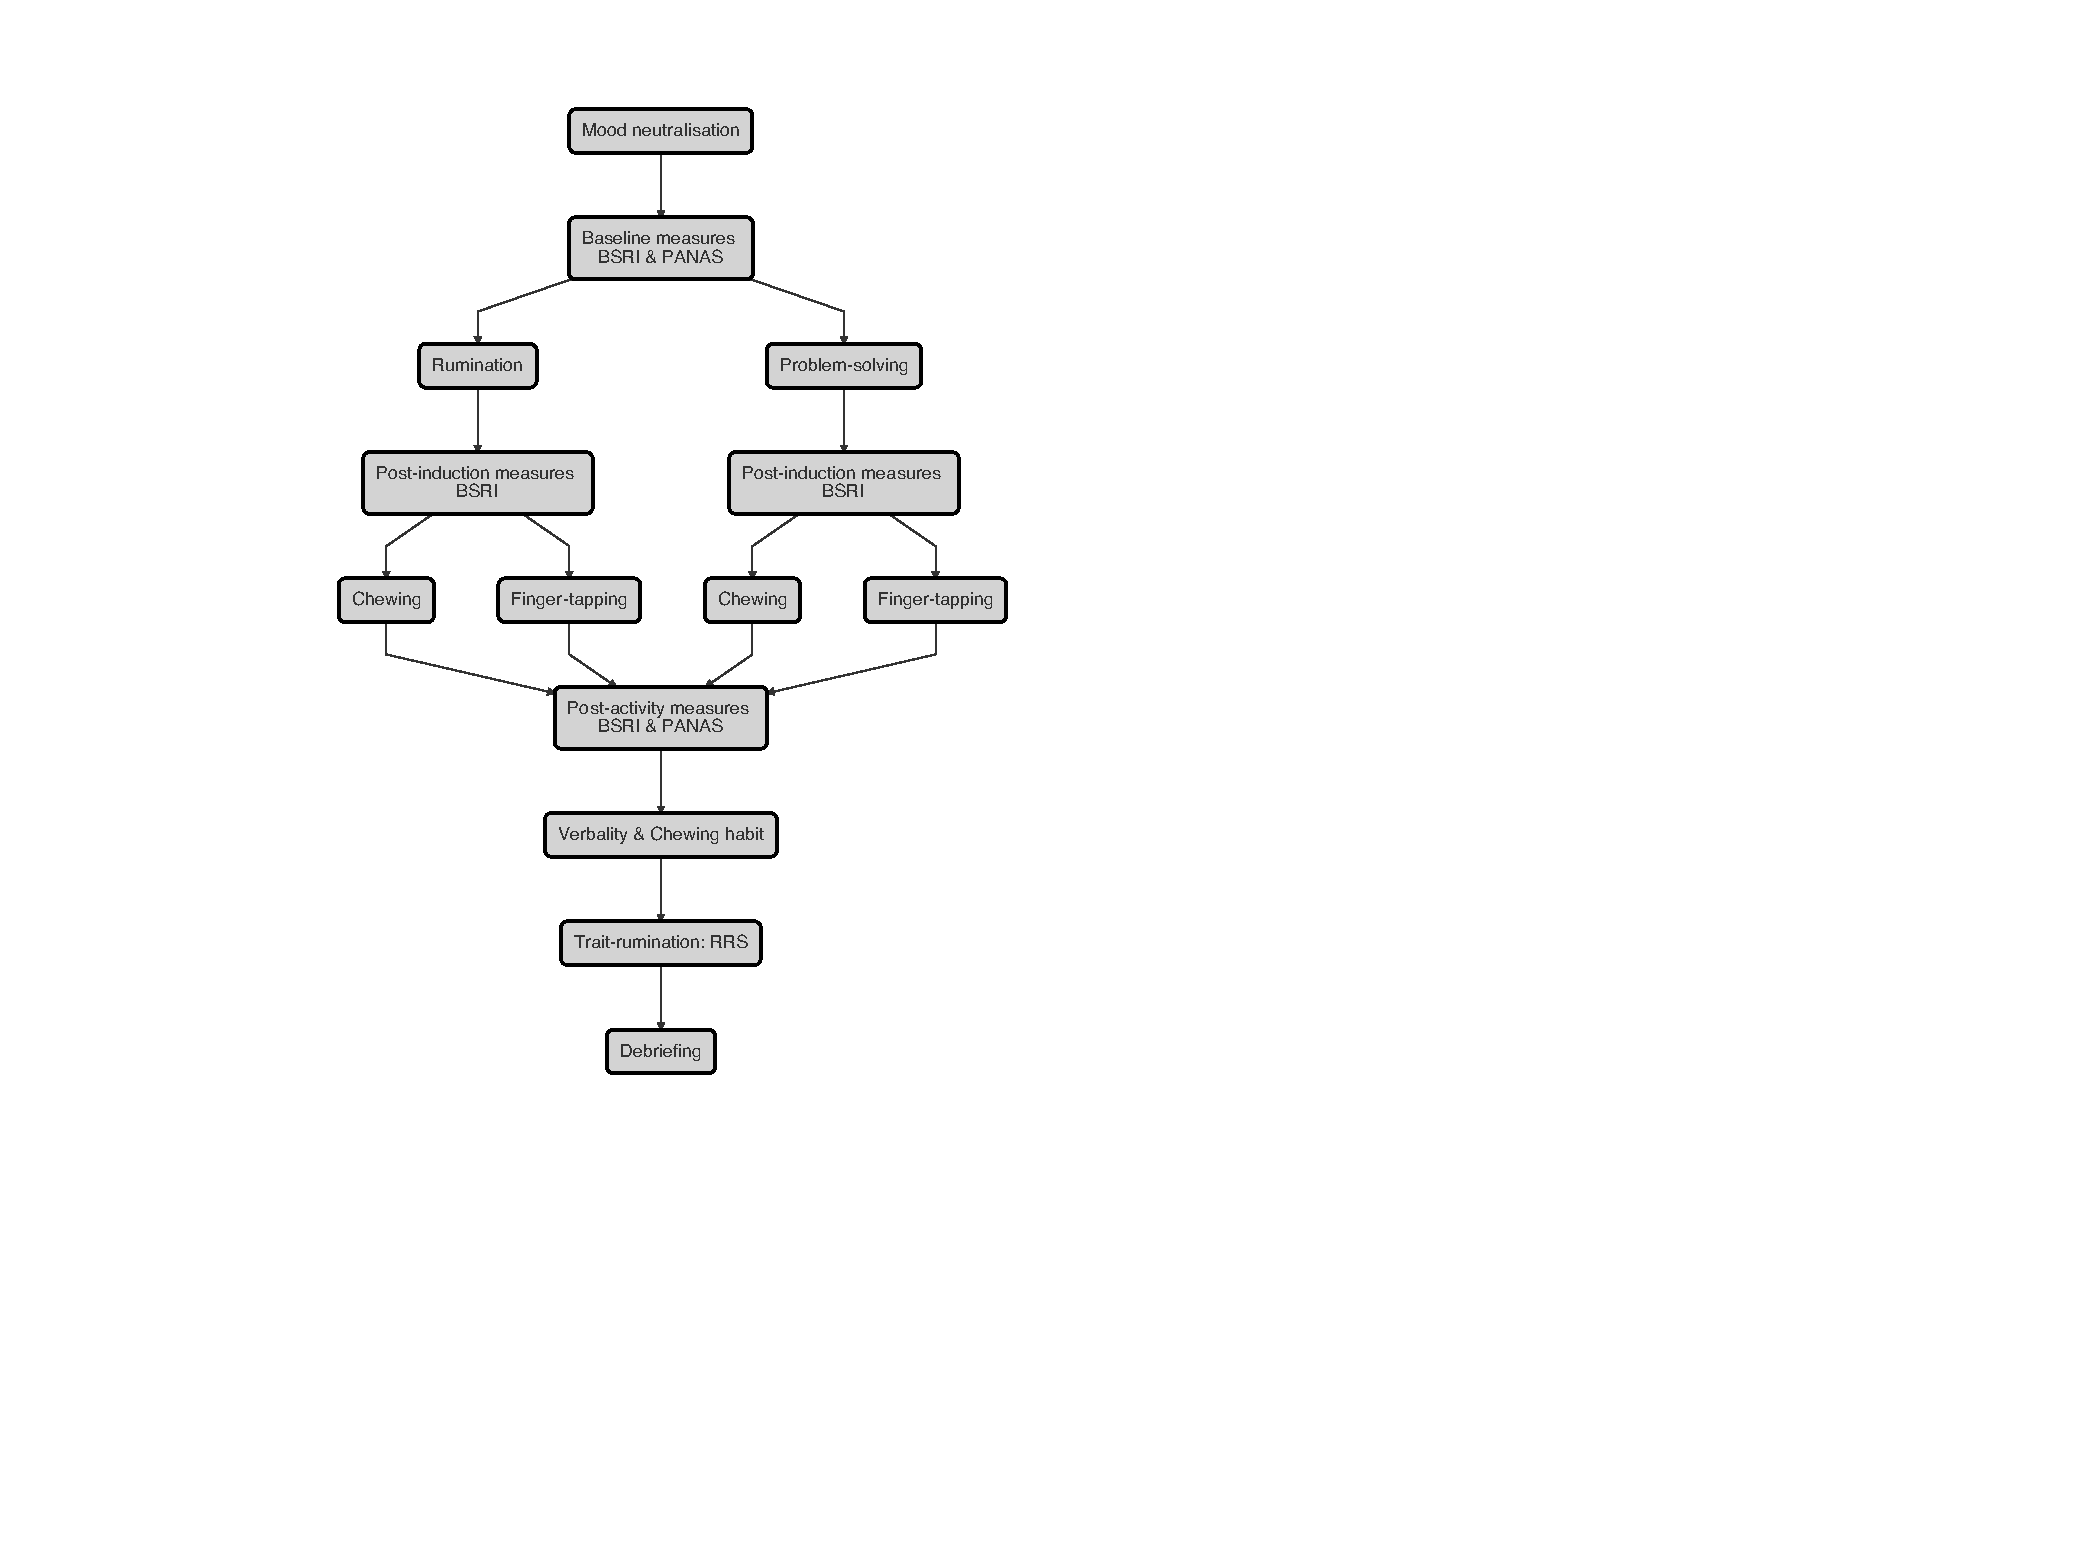
\includegraphics[width=0.66\linewidth]{07-chap7_files/figure-latex/diagramCh7-1} 

}

\caption{Timeline of the experiment, from top to bottom.}\label{fig:diagramCh7}
\end{figure}

\hypertarget{data-analysis-3}{%
\subsection{Data analysis}\label{data-analysis-3}}

Statistical analyses were conducted using \texttt{R} version 3.5.0 (R Core Team, \protect\hyperlink{ref-R-base}{2018}), and are reported with the \texttt{papaja} (Aust \& Barth, \protect\hyperlink{ref-R-papaja}{2018}) and \texttt{knitr} (Xie, \protect\hyperlink{ref-R-knitr}{2018}) packages.

To model state rumination and affect in response to the thinking-style induction and the articulatory suppression manipulation, we fitted a series of Bayesian regression models\footnote{An introduction to Bayesian statistical modelling is outside the scope of the current paper but the interested reader is referred to Nalborczyk et al. (\protect\hyperlink{ref-nalborczyk_introduction_2019}{2019}\protect\hyperlink{ref-nalborczyk_introduction_2019}{a}), for an introduction to Bayesian multilevel modelling using the \texttt{brms} package.}. These analyses were conducted using the \texttt{brms} package (Bürkner, \protect\hyperlink{ref-R-brms}{2018}), an implementation of Bayesian multilevel models that employs the probabilistic programming language \texttt{Stan} (Carpenter et al., \protect\hyperlink{ref-carpenter_stan_2017}{2017}). Four chains were run for each model, including each 10,000 iterations and a warmup of 2,000 iterations. Posterior convergence was assessed examining autocorrelation and trace plots, as well as the Gelman-Rubin statistic. Constant effects estimates were summarised via their posterior mean and 95\% credible interval (CrI), where a credible interval interval can be considered as the Bayesian analogue of a classical confidence interval, except that it can be interpreted in a probabilistic way (contrary to confidence intervals, Nalborczyk et al., \protect\hyperlink{ref-nalborczyk_pragmatism_2019}{2019}\protect\hyperlink{ref-nalborczyk_pragmatism_2019}{b}). When applicable, we also report Bayes factors (BFs) computed using the Savage-Dickey method.\footnote{This method simply consists in taking the ratio of the posterior density at the point of interest divided by the prior density at that point (Wagenmakers et al., \protect\hyperlink{ref-wagenmakers_bayesian_2010}{2010}).} These BFs can be interpreted as updating factors, from prior knowledge (what we knew before seeing the data) to posterior knowledge (what we know after seeing the data).

\hypertarget{results-4}{%
\section{Results}\label{results-4}}

The results section is divided into two sections investigating the effects of i) the thinking-style induction and ii) the interaction between the effect of the thinking-style induction (rumination vs.~problem-solving) and the effect of the motor activity (chewing vs.~finger-tapping) on self-reported state rumination and negative affects. Importantly, as data collection is still ongoing (it will continue next semester), these analyses should be considered as \emph{very preliminary}. The number of observations (participants) per condition is reported in Table \ref{tab:sampleszize}.

\begin{table}[H]
\begin{center}
\begin{threeparttable}
\caption{\label{tab:sampleszize}Current sample size per group.}
\begin{tabular}{llc}
\toprule
Thinking mode & Motor activity & Sample size\\
\midrule
problem-solving & chewing & 14\\
problem-solving & tapping & 8\\
rumination & chewing & 11\\
rumination & tapping & 9\\
\bottomrule
\end{tabular}
\end{threeparttable}
\end{center}
\end{table}

\hypertarget{thinking-style-induction-1}{%
\subsection{Thinking-style induction}\label{thinking-style-induction-1}}

To examine the efficiency of the induction procedure (i.e., the effects of time, coded as \emph{Session}, and the effects of the thinking-style, coded as \emph{Think}) while controlling for the other variables (i.e., \emph{RRSbrooding} and \emph{BDI.II}), we then compared the parsimony of several models containing different combinations of constant effects and a varying intercept for \emph{Participant}. Model comparison showed that the best model (i.e., the model with the lowest WAIC) was the model including \emph{Session} and \emph{BDI.II} as predictors (see Table \ref{tab:compexp1}). Fit of the best model was moderate (\(R^2\) = 0.577, 95\% CrI {[}0.377, 0.713{]}).

\begin{lltable}
\begin{TableNotes}[para]
\textit{Note.} $pWAIC$ is the number of effective parameters in the model. $Int$ = Intercept, $Ind$ = Induction, $RRSbro$ = RRSbrooding, $BDI$ = BDI-II score. All models include a varying intercept by participant.
\end{TableNotes}
\small{
\begin{longtable}{lcccc}\noalign{\getlongtablewidth\global\LTcapwidth=\longtablewidth}
\caption{\label{tab:compexp1}Comparison of models, ordered by WAIC relative to the best model (i.e., the model with the lowest WAIC).}\\
\toprule
 & \multicolumn{1}{c}{$WAIC$} & \multicolumn{1}{c}{$pWAIC$} & \multicolumn{1}{c}{$\Delta_{WAIC}$} & \multicolumn{1}{c}{$Weight$}\\
\midrule
$Int+Session+BDI$ & 1047.36 & 20.98 & 0.00 & 0.518\\
$Int+Session+BDI+Session:BDI$ & 1049.61 & 21.07 & 2.25 & 0.168\\
$Int+Session+RRSbro+BDI+Session:RRSbro+Session:BDI$ & 1050.63 & 21.80 & 3.27 & 0.101\\
$Int+Session+Think+Session:Think+BDI$ & 1051.16 & 20.42 & 3.80 & 0.078\\
$Int+Session+RRSbro$ & 1051.50 & 24.94 & 4.13 & 0.066\\
$Int+Session+RRSbro+Session:RRSbro$ & 1053.26 & 25.22 & 5.90 & 0.027\\
$Int+Session+Think+Session:Think+RRSbro$ & 1053.65 & 25.85 & 6.29 & 0.022\\
$Int+Session$ & 1054.52 & 27.54 & 7.16 & 0.014\\
$Int+Session+Think+Session:Think$ & 1056.27 & 28.31 & 8.91 & 0.006\\
\bottomrule
\addlinespace
\insertTableNotes
\end{longtable}
}
\end{lltable}

Constant effect estimates from the best model are reported in Table \ref{tab:paramexp1}. Based on these values, it seems that \emph{Session} (i.e., the effect of the rumination induction) increased self-reported state rumination (i.e., the BSRI sum score) by approximately 73.84 points on average (\(\beta\) = 73.844, 95\% CrI {[}31.982, 121.588{]}, \(BF10\) = 36.101). The main positive effect of \emph{BDI.II} indicates that higher BDI-II scores were associated with higher self-reported state rumination scores on average.

\begin{table}[H]
\begin{center}
\begin{threeparttable}
\caption{\label{tab:paramexp1}Coefficient estimates, standard errors (SE), 95\% CrI (Lower, Upper), Rhat, and Bayes factor (BF10) for the best model.}
\small{
\begin{tabular}{lcccccc}
\toprule
Term & \multicolumn{1}{c}{Estimate} & \multicolumn{1}{c}{SE} & \multicolumn{1}{c}{Lower} & \multicolumn{1}{c}{Upper} & \multicolumn{1}{c}{Rhat} & \multicolumn{1}{c}{BF10}\\
\midrule
Intercept & 235.309 & 15.667 & 205.005 & 267.664 & 1.000 & 5.712*10\textasciicircum{}18\\
Session & 73.844 & 22.819 & 31.982 & 121.588 & 1.000 & 36.1\\
BDI.II & 94.889 & 16.066 & 62.846 & 126.465 & 1.000 & 2.077*10\textasciicircum{}15\\
\bottomrule
\addlinespace
\end{tabular}
}
\begin{tablenotes}[para]
\textit{Note.} As all predictors were centered to the mean for analysis, these coefficients approximate coefficients from simpler models.
\end{tablenotes}
\end{threeparttable}
\end{center}
\end{table}

Model comparison revealed that the models including an interaction term between the effect of time (\emph{Session}) and the effect of the thinking-style (i.e., rumination vs.~problem-solving) were not ranked among the best models according to their WAIC (cf.~Table \ref{tab:compexp1}). However, for completeness, we report the estimations from the model including an effect of time, an effect of thinking-style, and an interaction between these two predictors (see Table \ref{tab:ParamInteraction}).

\begin{table}[H]
\begin{center}
\begin{threeparttable}
\caption{\label{tab:ParamInteraction}Coefficient estimates, standard errors (SE), 95\% CrI (Lower, Upper), Rhat, and Bayes factor (BF10) for the model including an interaction between session and thinking-style.}
\small{
\begin{tabular}{lcccccc}
\toprule
Term & \multicolumn{1}{c}{Estimate} & \multicolumn{1}{c}{SE} & \multicolumn{1}{c}{Lower} & \multicolumn{1}{c}{Upper} & \multicolumn{1}{c}{Rhat} & \multicolumn{1}{c}{BF10}\\
\midrule
Intercept & 235.656 & 22.237 & 192.689 & 279.077 & 1.001 & 9.728*10\textasciicircum{}16\\
Session & 74.491 & 21.980 & 29.397 & 118.635 & 1.000 & 31.01\\
Thinking mode & -9.729 & 41.109 & -83.959 & 76.537 & 1.000 & 0.411\\
Session x Thinking mode & 3.299 & 41.764 & -78.797 & 87.723 & 1.000 & 0.388\\
\bottomrule
\addlinespace
\end{tabular}
}
\begin{tablenotes}[para]
\textit{Note.} As all predictors were centered to the mean for analysis, these coefficients approximate coefficients from simpler models.
\end{tablenotes}
\end{threeparttable}
\end{center}
\end{table}

This analysis revealed that both the thinking-style (i.e., rumination vs.~problem-solving) and the interaction between time and thinking-style have a negligible effect on self-reported state rumination (\(\beta\) = 3.299, 95\% CrI {[}-78.797, 87.723{]}, \(BF10\) = 0.388). In other words, the rumination induction was not associated with more self-reported state rumination than the problem-solving induction (although more rumination was reported after induction than before on average).

\hypertarget{articulatory-suppression-effects-2}{%
\subsection{Articulatory suppression effects}\label{articulatory-suppression-effects-2}}

\hypertarget{self-reported-state-rumination}{%
\subsubsection{Self-reported state rumination}\label{self-reported-state-rumination}}

We then examined the effect of the two motor tasks (gum-chewing vs.~finger-tapping) on both self-reported state rumination (BSRI) and self-reported negative affects (the negative dimension of the PANAS), while controlling for the amount of verbal thoughts reported by the participant. Based on our hypotheses, we expected that the model comparison would reveal a three-way interaction between Session, Thinking-style and the type of motor activity. However, the best model identified by the WAIC model comparison did not include this interaction as a constant effect (see Table \ref{tab:compexp2}). Fit of the best model was moderate (\(R^2\) = 0.73, 95\% CrI {[}0.6, 0.81{]}).

\begin{lltable}
\begin{TableNotes}[para]
\textit{Note.} $pWAIC$ is the number of effective parameters in the model. $Int$ = Intercept, $Ind$ = Induction, $RRSbro$ = RRSbrooding, $BDI$ = BDI-II score. All models include a varying intercept by participant.
\end{TableNotes}
\small{
\begin{longtable}{lcccc}\noalign{\getlongtablewidth\global\LTcapwidth=\longtablewidth}
\caption{\label{tab:compexp2}Comparison of models, ordered by WAIC relative to the best model (i.e., the model with the lowest WAIC).}\\
\toprule
 & \multicolumn{1}{c}{$WAIC$} & \multicolumn{1}{c}{$pWAIC$} & \multicolumn{1}{c}{$\Delta_{WAIC}$} & \multicolumn{1}{c}{$Weight$}\\
\midrule
$Int+Session$ & 1018.85 & 30.04 & 0.00 & 0.467\\
$Int+Session+Think+Session:Think$ & 1020.55 & 30.43 & 1.69 & 0.200\\
$Int+Session+Motor+Verbal+Session:Motor+Session:Verbal+Session:Motor:Verbal$ & 1020.75 & 30.63 & 1.89 & 0.181\\
$Int+Session+Motor+Session:Motor$ & 1021.74 & 30.43 & 2.88 & 0.111\\
$Int+Session+Motor+Think+Session:Motor+Session:Think+Session:Motor:Think$ & 1024.97 & 31.13 & 6.11 & 0.022\\
$Full model$ & 1025.31 & 32.14 & 6.46 & 0.019\\
\bottomrule
\addlinespace
\insertTableNotes
\end{longtable}
}
\end{lltable}

However, because we are interested in estimating the effect of each predictor (and because the amount of data is very low), we report the estimations from the model including an effect of time, motor activity, verbality, as well as two-way and three-way interactions between these predictors. Constant effect estimates for this model are reported in Table \ref{tab:paramexp2}. Based on these values, it seems that the overall self-reported levels of state rumination did not decrease after motor activity (\(\beta\) = 0.676, 95\% CrI {[}-37.094, 38.605{]}, \(BF10\) = 0.189). However, \emph{Verbality} (i.e., the amount of verbal thoughts) was positively associated with state rumination on average (\(\beta\) = 66.857, 95\% CrI {[}26.811, 109.706{]}, \(BF10\) = 20.863). Interestingly, the interaction between session, motor activity, and verbality indicates that a higher amount of verbal thoughts was associated with a \emph{different} interaction between session and motor activity (\(\beta\) = 51.744, 95\% CrI {[}-17.598, 122.822{]}, \(BF10\) = 1.03). As three-way interaction effects are better understood visually, we depict this effect in Figure \ref{fig:interactionplot}. This figure shows that higher amounts of verbal thoughts were associated with lower levels of self-reported state rumination in the chewing group and higher levels of self-reported state rumination in the finger-tapping group (as we predicted). However, the estimation of this effect is very uncertain due to the low sample size (as expressed by the large standard error) and should be therefore considered cautiously.\footnote{Moreover, the relation between the verbal scale and the change in self-reported state rumination following the motor activity looks only vaguely linear, which should make us cautious about the interpretation of the linear estimates.} The overall evolution of self-reported state rumination throughout the experiment by condition is depicted in Figure \ref{fig:bsriplot}.

\begin{table}[H]
\begin{center}
\begin{threeparttable}
\caption{\label{tab:paramexp2}Coefficient estimates, standard errors (SE), 95\% CrI (Lower, Upper), Rhat and Bayes factor (BF10) for the best model.}
\small{
\begin{tabular}{lcccccc}
\toprule
Term & \multicolumn{1}{c}{Estimate} & \multicolumn{1}{c}{SE} & \multicolumn{1}{c}{Lower} & \multicolumn{1}{c}{Upper} & \multicolumn{1}{c}{Rhat} & \multicolumn{1}{c}{BF10}\\
\midrule
Intercept & 281.734 & 21.897 & 239.382 & 325.671 & 1.000 & 3.926*10\textasciicircum{}16\\
Session & 0.676 & 19.095 & -37.094 & 38.605 & 1.000 & 0.189\\
Motor activity & 47.311 & 39.246 & -29.454 & 128.321 & 1.000 & 0.817\\
Verbality & 66.857 & 21.140 & 26.811 & 109.706 & 1.000 & 20.86\\
Session x Motor activity & -7.447 & 36.080 & -81.044 & 61.762 & 1.000 & 0.37\\
Session x Verbality & -6.710 & 19.027 & -43.507 & 31.497 & 1.000 & 0.199\\
Motor activity x Verbality & 39.678 & 40.836 & -36.093 & 123.728 & 1.000 & 0.633\\
Session x Motor activity x Verbality & 51.744 & 35.428 & -17.598 & 122.822 & 1.000 & 1.03\\
\bottomrule
\addlinespace
\end{tabular}
}
\begin{tablenotes}[para]
\textit{Note.} As all predictors were centered to the mean for analysis, these coefficients approximate coefficients from simpler models.
\end{tablenotes}
\end{threeparttable}
\end{center}
\end{table}

\begin{figure}

{\centering 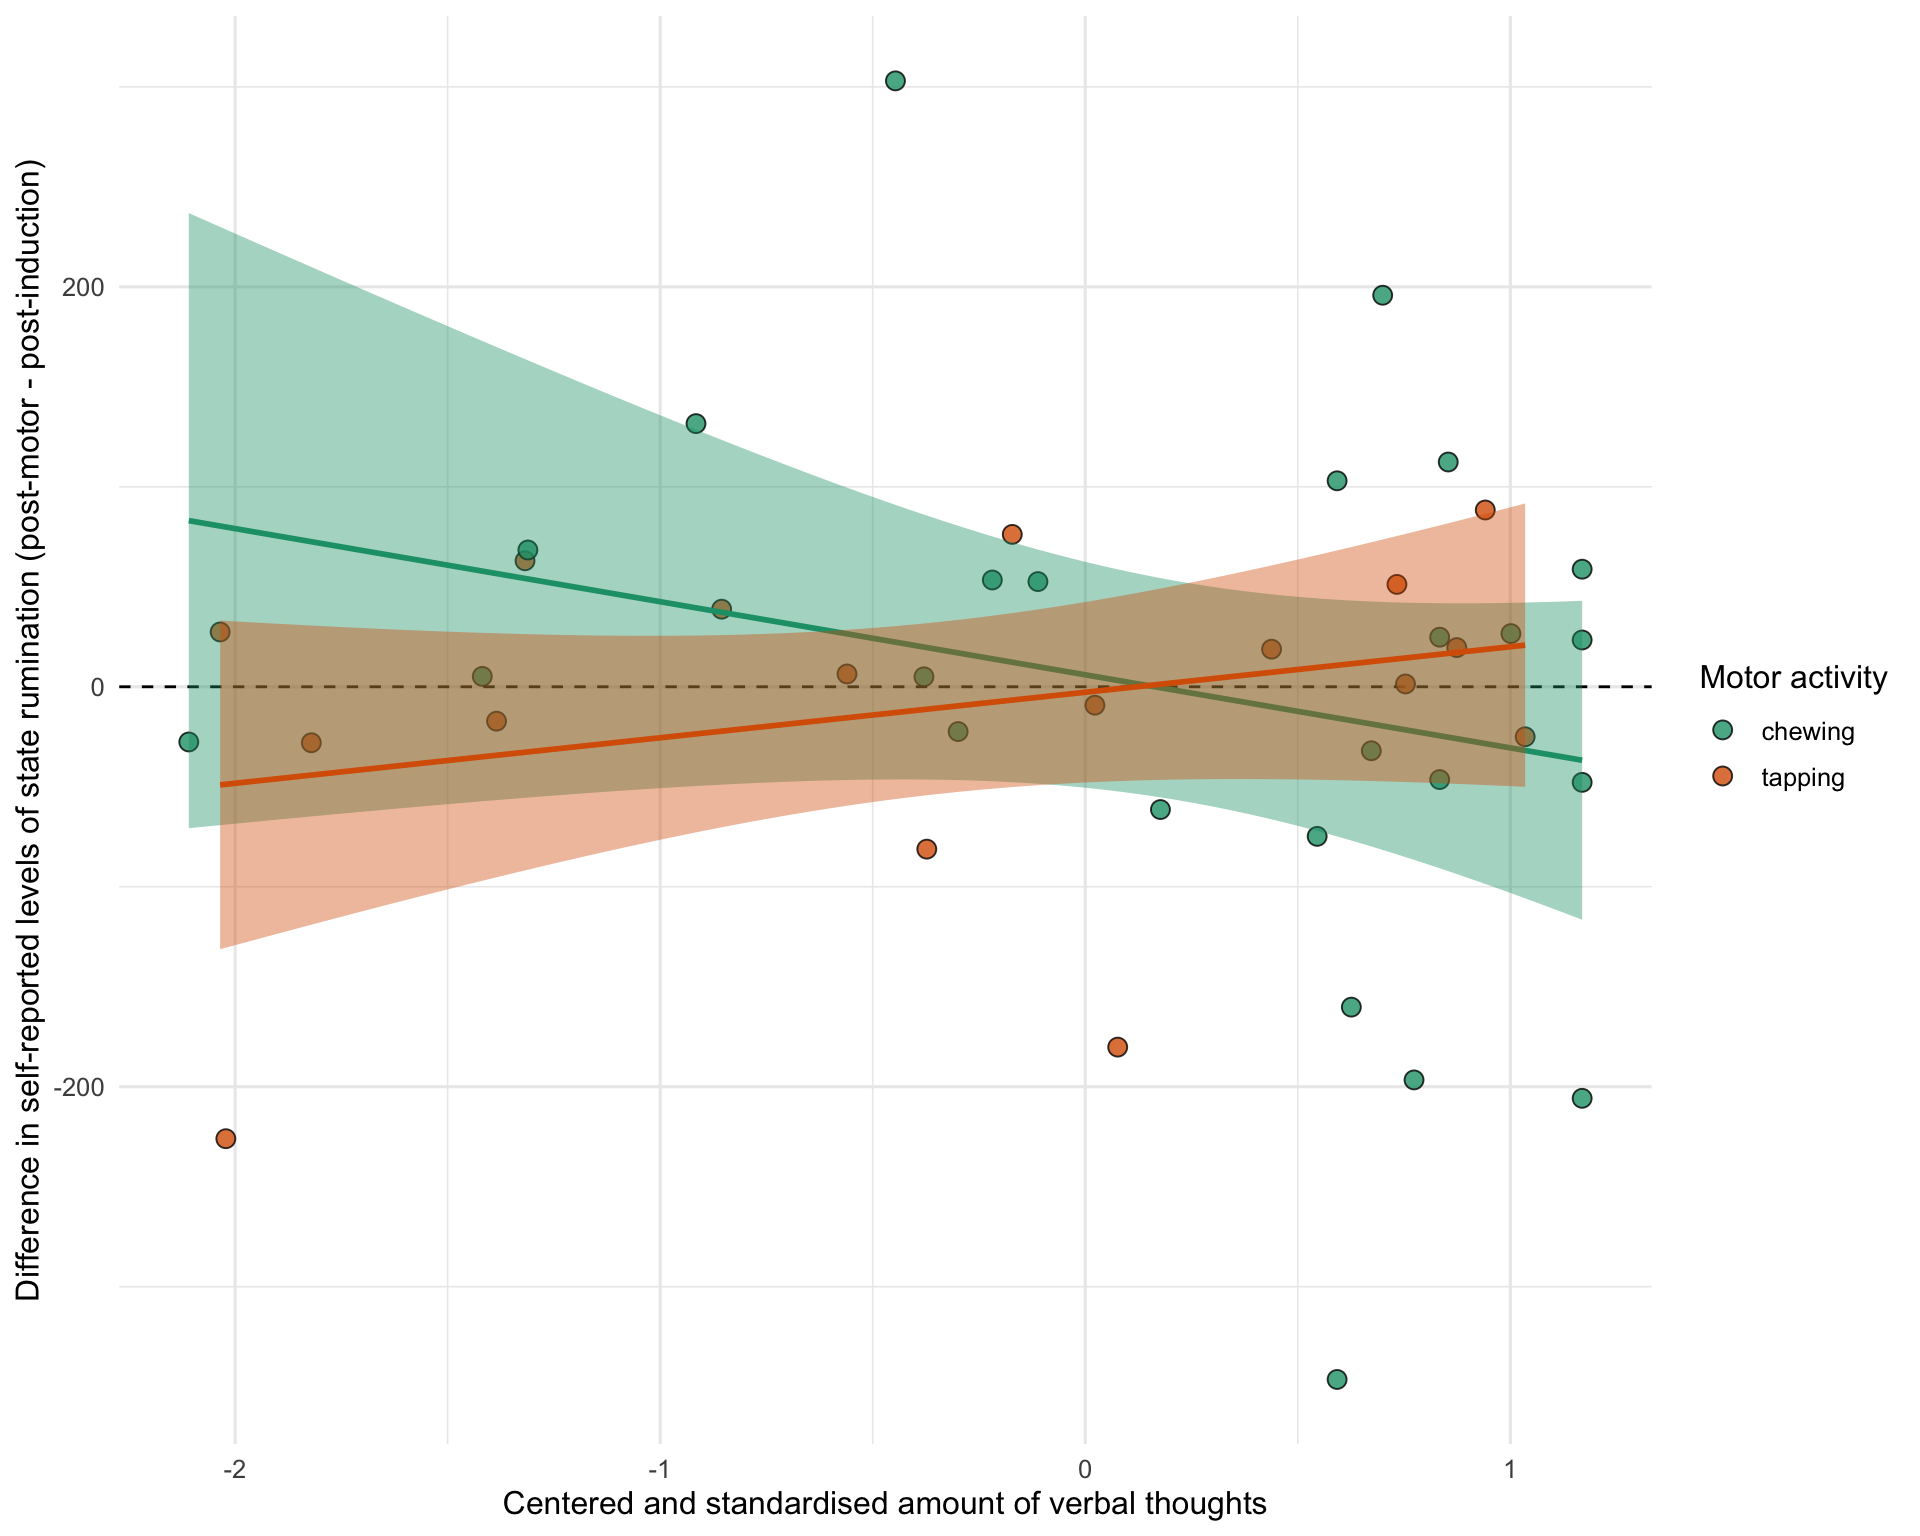
\includegraphics[width=1\linewidth]{07-chap7_files/figure-latex/interactionplot-1} 

}

\caption{Interaction between session, motor activity, and verbality. The x-axis represents the amount of verbal thoughts reported by the participant. The y-axis represents differences in self-reported state rumination from after the induction to after the motor activity. Dots represent individual scores.}\label{fig:interactionplot}
\end{figure}

\begin{figure}

{\centering 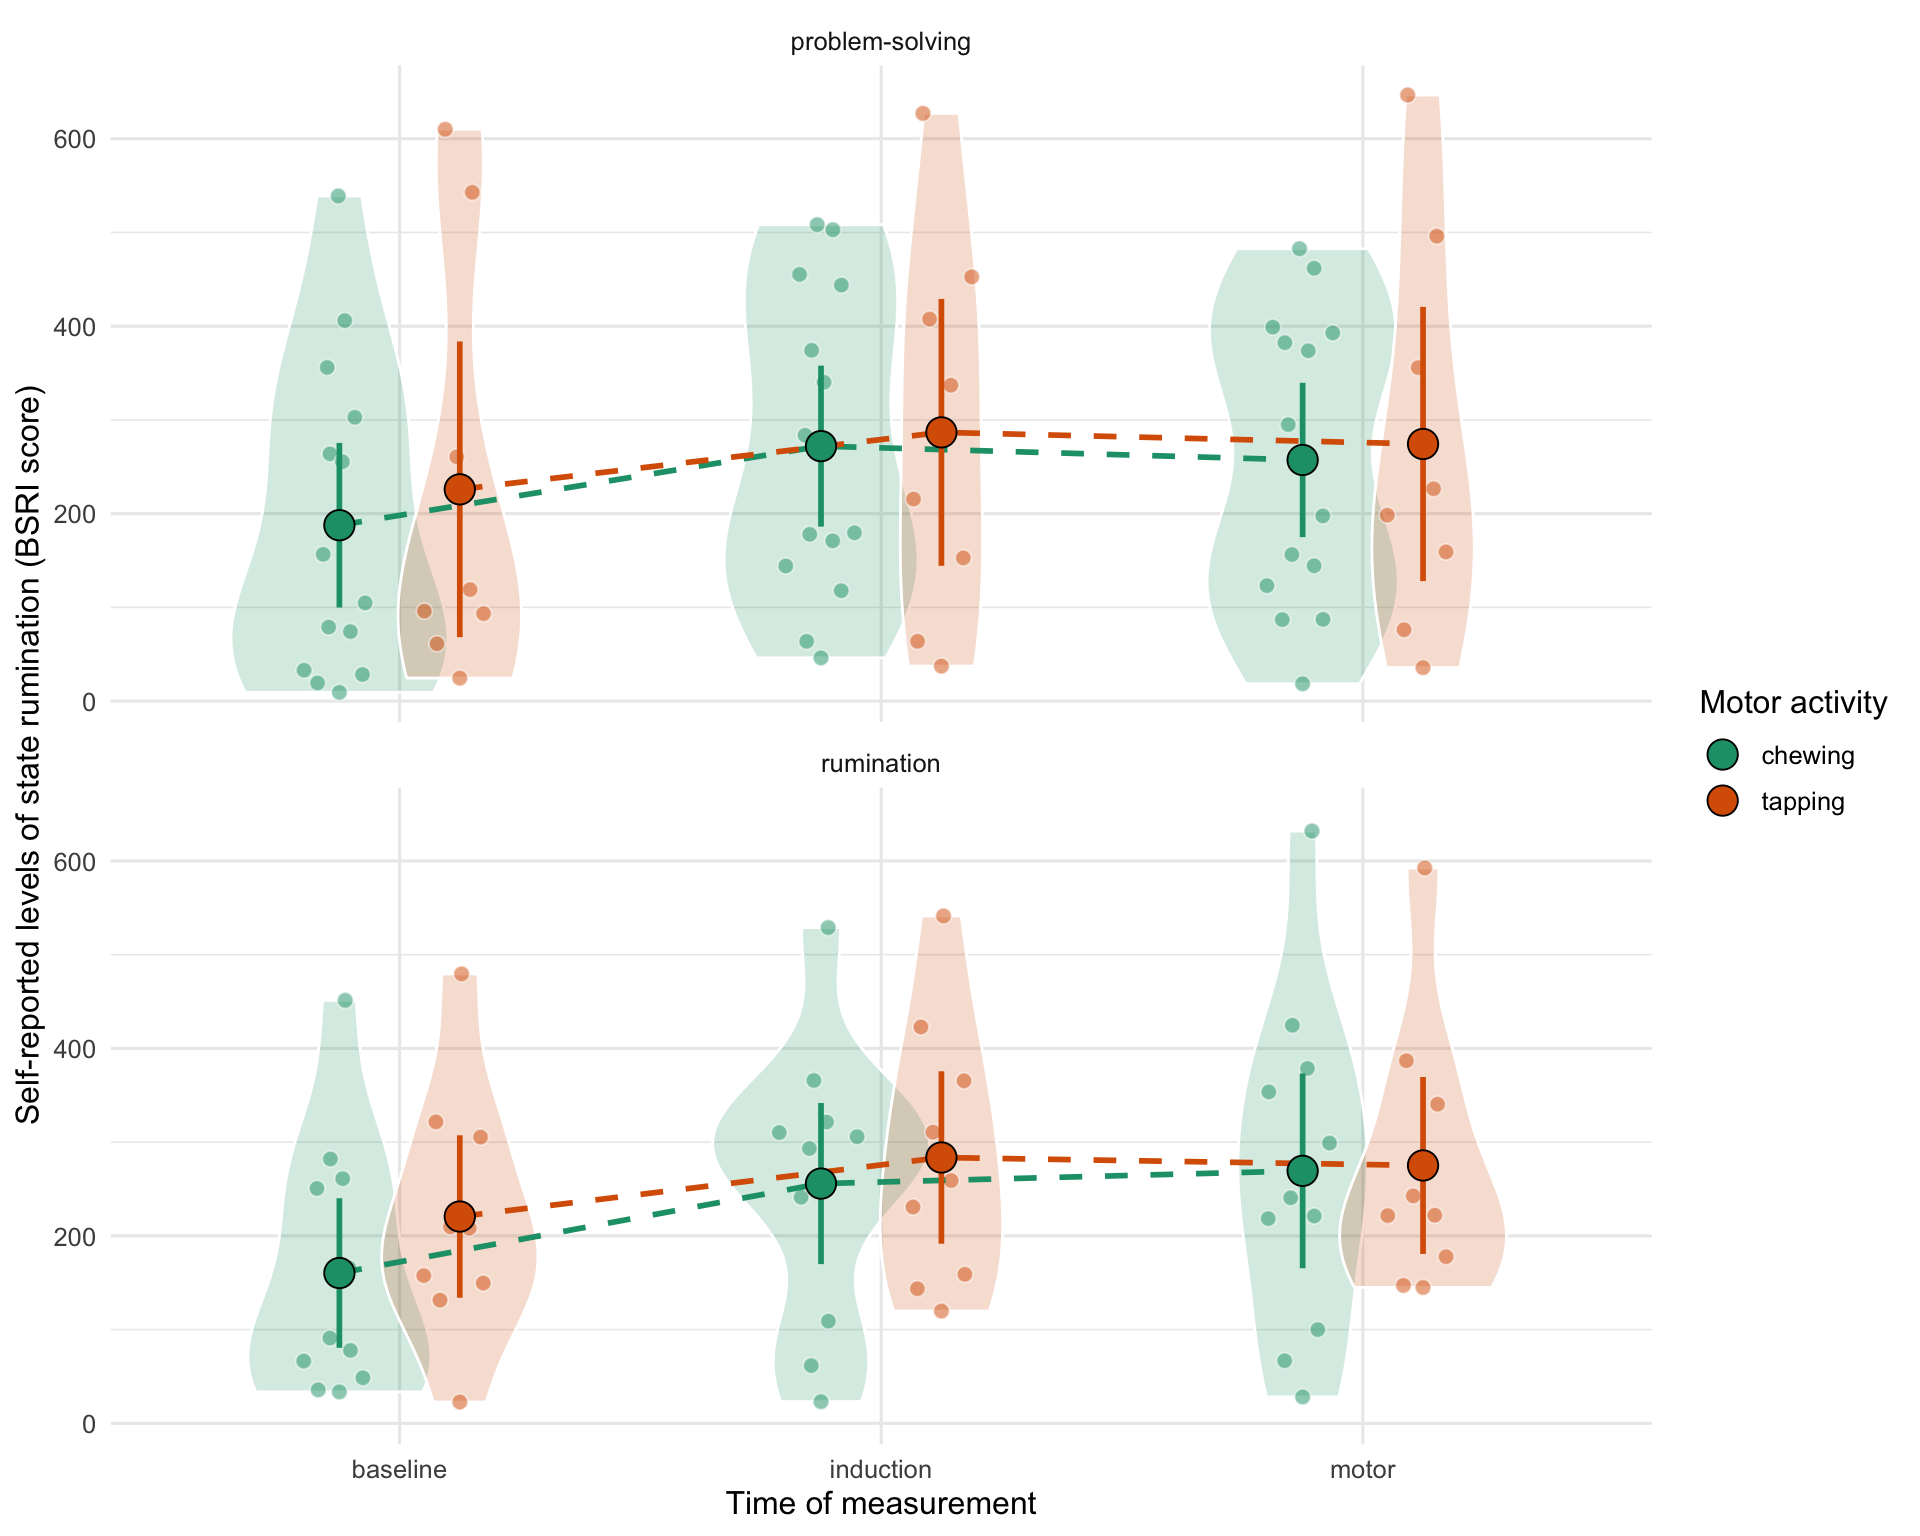
\includegraphics[width=1\linewidth]{07-chap7_files/figure-latex/bsriplot-1} 

}

\caption{Average self-reported levels of state rumination (BSRI sum score) throughout the experiment, by thinking-style and type of motor activity. Smaller dots represent individual scores.}\label{fig:bsriplot}
\end{figure}

\hypertarget{self-reported-negative-affects}{%
\subsubsection{Self-reported negative affects}\label{self-reported-negative-affects}}

In addition to the self-reported levels of state rumination after each type of motor activity, we were also interested in the self-reported levels of state negative affects. More precisely, we expected an interaction between the type of motor activity (chewing vs.~finger-tapping) and the thinking-style (rumination vs.~problem-solving). Indeed, as both rumination and problem-solving are expected to recruit inner speech to some extent, we expected both thinking styles to be affected by articulatory suppression (i.e., by gum-chewing). Because rumination is expected to have detrimental effects on mood (assessed via the PANAS score) and problem-solving is expected to have \enquote{less detrimental} effects (in comparison to rumination), interfering with these thinking styles should reduce their effect on mood. To assess this effect, we examined the interaction effect between thinking-style and motor activity on the change in negative affects from baseline to after the motor activity (in other words, on the baseline-normalised PANAS score). These data are depicted in Figure \ref{fig:panasplot}.

\begin{figure}

{\centering 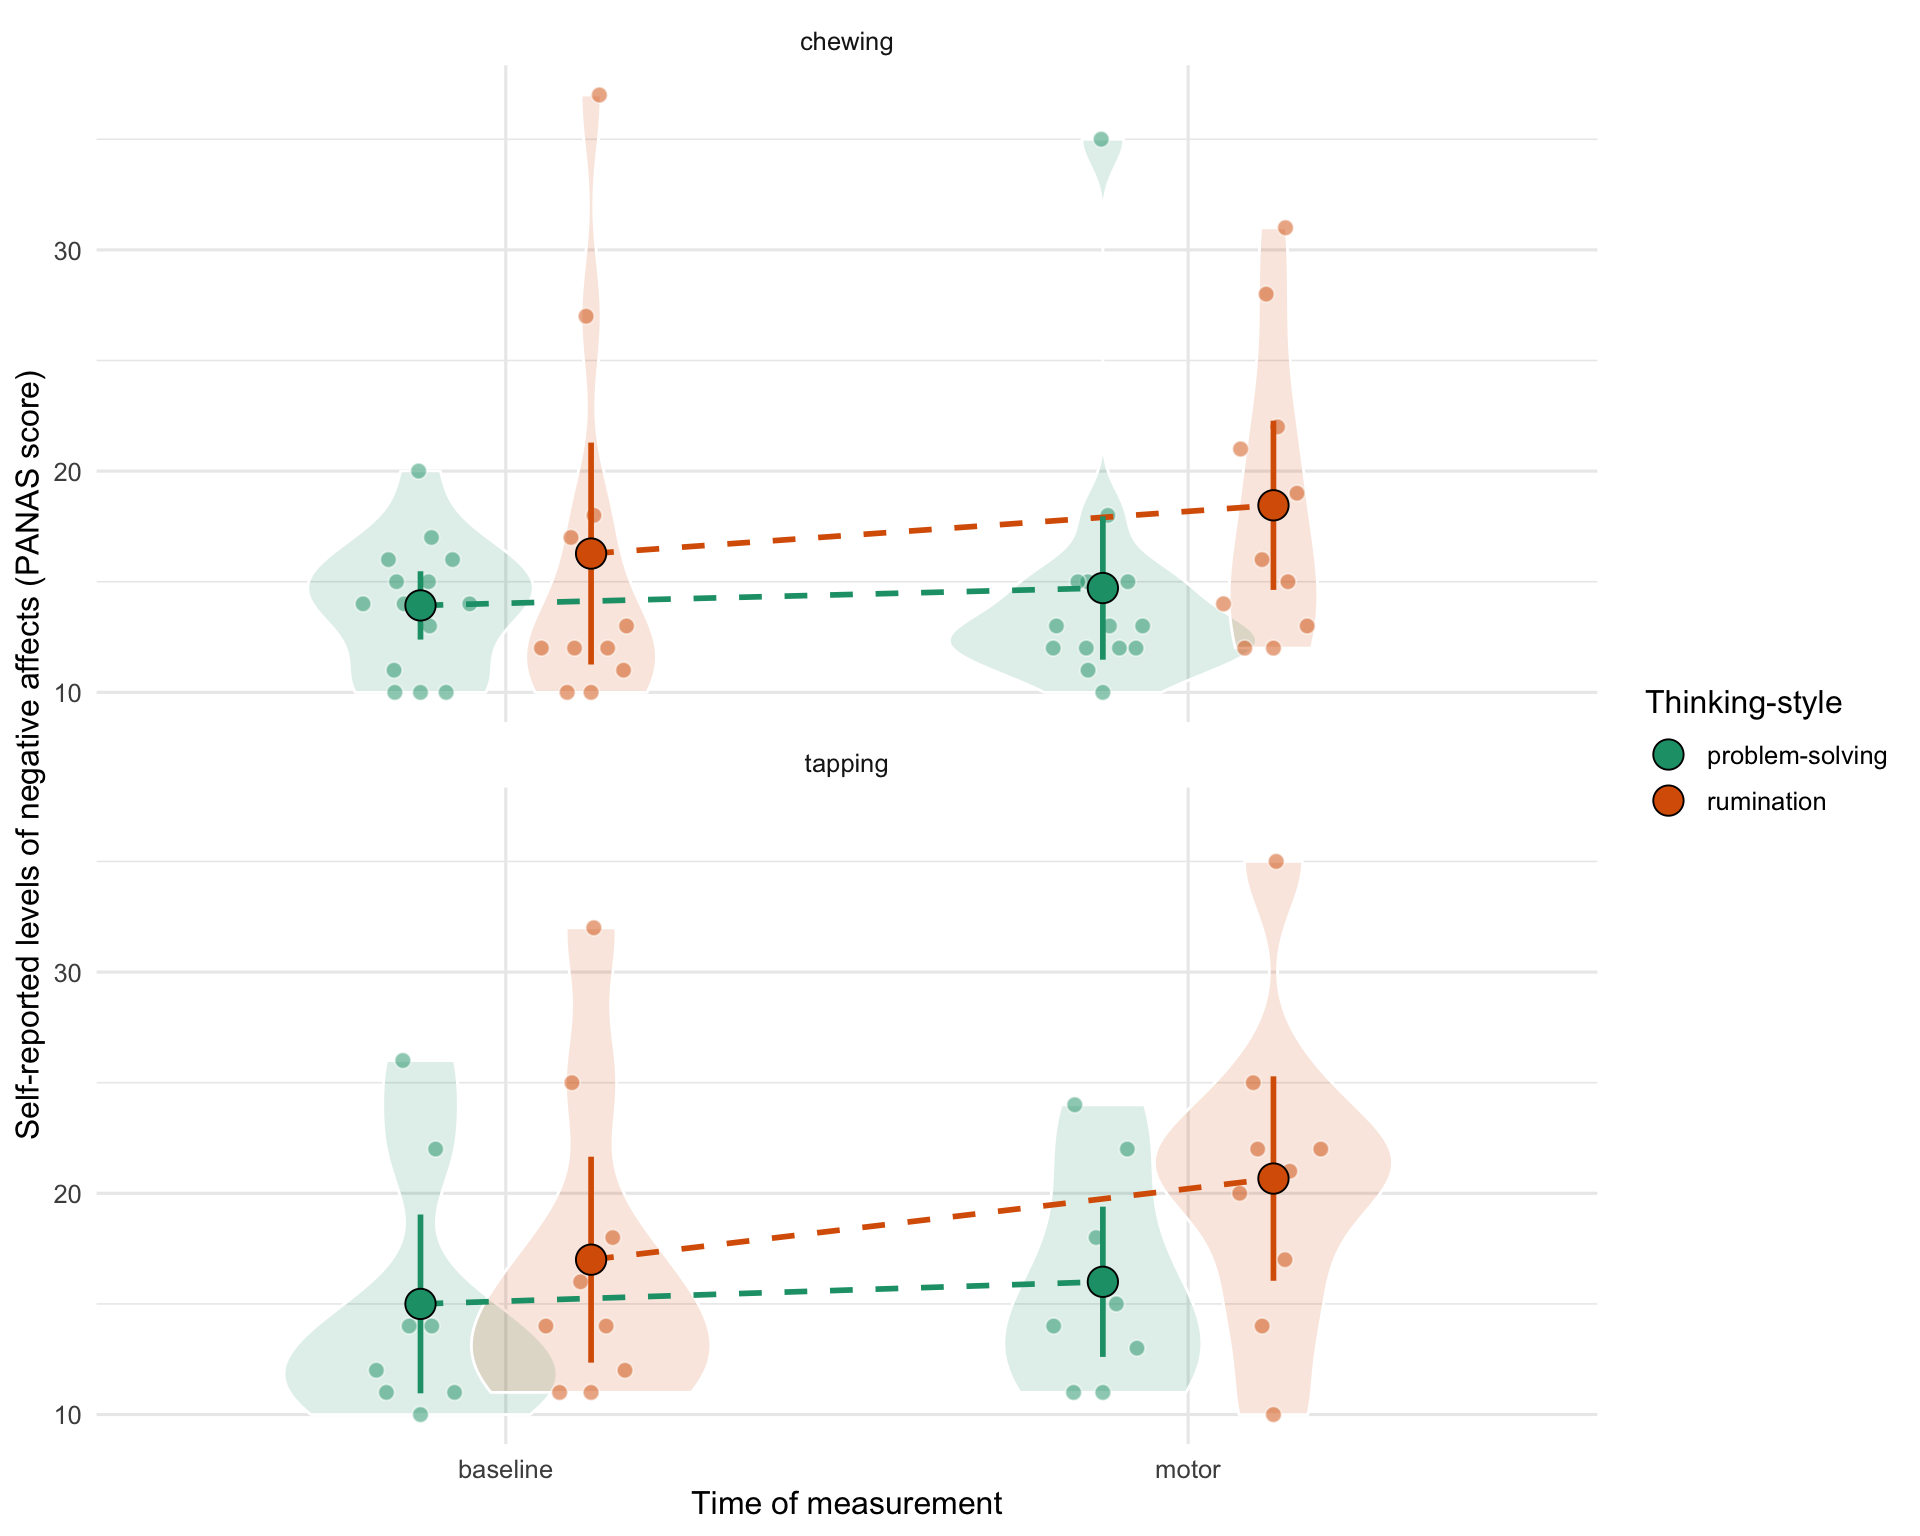
\includegraphics[width=1\linewidth]{07-chap7_files/figure-latex/panasplot-1} 

}

\caption{Average self-reported levels of state negative affects (PANAS) by thinking style and type of motor activity at the beginning (baseline) and end (motor) of the experiment. Smaller dots represent individual scores. NB: colouring and facetting factors have been reversed as compared to the BSRI figure to better highlight the interaction effect.}\label{fig:panasplot}
\end{figure}

As previously, we compared several models to examine our hypotheses. Based on our hypotheses, we expected that the model comparison would reveal a three-way interaction between Thinking-style and the type of motor activity. However, the best model identified by the WAIC model comparison did not include this interaction as a constant effect (see Table \ref{tab:compexp2panas}).

\begin{lltable}
\begin{TableNotes}[para]
\textit{Note.} $pWAIC$ is the number of effective parameters in the model. $Int$ = Intercept, $Ind$ = Induction, $RRSbro$ = RRSbrooding, $BDI$ = BDI-II score. All models include a varying intercept by participant.
\end{TableNotes}
\small{
\begin{longtable}{lcccc}\noalign{\getlongtablewidth\global\LTcapwidth=\longtablewidth}
\caption{\label{tab:compexp2panas}Comparison of models, ordered by WAIC relative to the best model (i.e., the model with the lowest WAIC).}\\
\toprule
 & \multicolumn{1}{c}{$WAIC$} & \multicolumn{1}{c}{$pWAIC$} & \multicolumn{1}{c}{$\Delta_{WAIC}$} & \multicolumn{1}{c}{$Weight$}\\
\midrule
$Int$ & 264.74 & 3.63 & 0.00 & 0.397\\
$Int+Think$ & 265.42 & 4.59 & 0.69 & 0.281\\
$Int+Motor$ & 266.15 & 4.34 & 1.42 & 0.195\\
$Int+Think+Motor+Think:Motor$ & 268.28 & 5.41 & 3.55 & 0.067\\
$Int+Motor+Verbal+Motor:Verbal$ & 268.68 & 5.96 & 3.95 & 0.055\\
$Full\ model$ & 273.88 & 7.98 & 9.15 & 0.004\\
\bottomrule
\addlinespace
\insertTableNotes
\end{longtable}
}
\end{lltable}

However, because we are interested in estimating the effect of each predictor (and because these analyses are still preliminary), we report the estimations from the full model (i.e., the model including an effect of thinking-style, motor activity and verbality as well as all possible interaction effects) in Table \ref{tab:paramexp2panas}. Based on these values, it seems that self-reported levels of negative affects increased from baseline to the end of the experiment (\(\beta\) = 2.021, 95\% CrI {[}0.178, 3.88{]}, \(BF10\) = 0.874). Moreover, the rumination induction lead to a greater increase in negative affects than the problem-solving induction (\(\beta\) = 1.931, 95\% CrI {[}-1.653, 5.699{]}, \(BF10\) = 0.344), and the chewing groups also showed a greater increase in negative affects as compared to the finger-tapping groups (\(\beta\) = 1.086, 95\% CrI {[}-2.594, 4.599{]}, \(BF10\) = 0.216). Interestingly, the interaction between thinking-style and motor activity indicates that the effect of the motor activity on the change in negative affect was different according to the thinking-style (\(\beta\) = 1.271, 95\% CrI {[}-6.048, 8.175{]}, \(BF10\) = 0.373). As three-way interaction effects are better understood visually, we depict this effect in Figure \ref{fig:panasplot}. This figure shows that the effect of the thinking-style on the change in self-reported state negative affects (i.e., the difference in steepness of the regression lines) was different according to the type of motor activity, with a stronger effect of the thinking-style in the finger-tapping condition than in the chewing condition (as we predicted). However, the estimation of these effects is very uncertain due to the low sample size (as expressed by the large standard error) and should therefore be considered cautiously.

\begin{table}[H]
\begin{center}
\begin{threeparttable}
\caption{\label{tab:paramexp2panas}Coefficient estimates, standard errors (SE), 95\% CrI (Lower, Upper), Rhat, and Bayes factor (BF10) for the best model.}
\small{
\begin{tabular}{lcccccc}
\toprule
Term & \multicolumn{1}{c}{Estimate} & \multicolumn{1}{c}{SE} & \multicolumn{1}{c}{Lower} & \multicolumn{1}{c}{Upper} & \multicolumn{1}{c}{Rhat} & \multicolumn{1}{c}{BF10}\\
\midrule
Intercept & 2.021 & 0.925 & 0.178 & 3.880 & 1.000 & 0.874\\
Thinking-style & 1.931 & 1.804 & -1.653 & 5.699 & 1.000 & 0.344\\
Motor activity & 1.086 & 1.808 & -2.594 & 4.599 & 1.000 & 0.216\\
Verbality & 0.819 & 0.910 & -0.908 & 2.714 & 1.000 & 0.14\\
Thinking-style x Motor activity & 1.271 & 3.433 & -6.048 & 8.175 & 1.000 & 0.373\\
Thinking-style x Verbality & 1.364 & 1.821 & -2.323 & 4.910 & 1.000 & 0.237\\
Motor activity x Verbality & 0.807 & 1.839 & -2.693 & 4.552 & 1.000 & 0.199\\
Thinking-style x Motor activity x Verbality & 0.529 & 3.453 & -6.710 & 7.580 & 1.000 & 0.359\\
\bottomrule
\addlinespace
\end{tabular}
}
\begin{tablenotes}[para]
\textit{Note.} As all predictors were centered to the mean for analysis, these coefficients approximate coefficients from simpler models.
\end{tablenotes}
\end{threeparttable}
\end{center}
\end{table}

\hypertarget{discussion-4}{%
\section{Discussion}\label{discussion-4}}

The discussion section will be completed once data will be fully gathered and analysed.

\hypertarget{supp}{%
\section{Supplementary materials}\label{supp}}

Pre-registered protocol, open data, supplementary analyses as well as reproducible code and figures are available at \url{https://osf.io/8ab2d/}.

\hypertarget{acknowledgements-4}{%
\section{Acknowledgements}\label{acknowledgements-4}}

The first author is funded by a PhD fellowship from Univ. Grenoble Alpes. We thank Kim Rens for her help during data collection.

\newpage

\begin{vplace}[1]

\begin{summary}{Summary of Chapter\getcurrentref{chapter}}

In this chapter, we extended the experiment from Chapter 6 by comparing the effects of articulatory suppression (vs. finger-tapping) on rumination and problem-solving, another (more adaptive) form of repetitive thinking. To overcome the limitations of the previous experiment, we used a validated scale of state rumination and asked our participants to use their non-dominant forearm in the finger-tapping condition. We also made sure that our baseline measurements were not contaminated by any systematic effect. The data collection for this experiment is still ongoing and given the very low sample size (around 10 participants per group at the time of writing), we will not consider these results further in the discussion. However, preliminary analyses presented in the results section suggest that articulatory suppression may indeed interfere with induced rumination.

\end{summary}

\end{vplace}

\hypertarget{part-discussion-and-conclusion}{%
\part{Discussion and conclusion}\label{part-discussion-and-conclusion}}

\hypertarget{chap8}{%
\chapter{Discussion and perspectives}\label{chap8}}

\initial{S}everal lines of research have suggested that inner speech may recruit speech motor processes. This work includes introspective and phenomenological studies, mental chronometry studies, motor interference studies, modelling work as well as neurophysiological and psychophysiological studies (cf.~our short historical review in Chapter \ref{intro}). However, the involvement of motor processes during inner speech is highly variable between individuals, tasks, and studies. Therefore, it seems reasonable to assume that inner speech comes in different \emph{varieties} that may involve speech motor processes to a variable extent. We tested this assumption by examining the involvement of the speech motor system during induced rumination, a negative and repetitive form of inner speech. In addition to shedding light upon the nature of inner speech, this work may offer new theoretical and experimental tools to assess the presence and persistence of ruminative thoughts.

\hypertarget{summary}{%
\section{Summary of the results}\label{summary}}

As argued in Chapter \ref{intro}, the guiding assumption underlying this work was that (verbal) rumination may be considered as a form of inner speech. Honouring that assumption, we studied induced rumination with the tools and methods used to investigate the phenomenon of inner speech. In the first experimental chapter (Chapter \ref{chap3}), we used surface EMG to assess the predictions of two competing views of inner speech production. According to the \emph{motor simulation view}, inner speech would be similar to overt speech, except that final execution of the speech actions is inhibited. Therefore, it should be possible to record peripheral muscular activation in the speech muscles during inner speech. According to the \emph{abstraction view}, the level of truncation between overt speech and inner speech would be located higher in the sense that inner speech would not include articulatory features. Therefore, under this view, it is not expected to record peripheral muscular activation in the speech muscles during inner speech. We observed that the induction of rumination was accompanied with increased EMG amplitude in all facial muscles (i.e., orbicularis oris inferior, orbicularis oris superior and frontalis) as compared to rest. It should be noted that baseline recordings were performed after a relaxation session. We interpreted these findings as a corroboration of the motor simulation view, with the activity of the speech muscles increasing from baseline to after the induction, suggesting that rumination, as a form of inner speech, may involve the speech motor system. We interpreted the increased activation of the forehead muscle as a consequence of the negative content of rumination, as the frontalis muscle is known to be associated with the expression of anger and sadness. Additionally, in the second part of this experiment, we observed that a relaxation focused on the speech muscles was slightly more efficient than a relaxation focused on the arm in reducing self-reported state rumination. However, a few important limitations are worth keeping in mind when considering these results. First, as we did not have any control group for the rumination induction, it is adventurous to attribute the observed effects to the rumination induction only.\footnote{More precisely, concluding \(p\) on the basis of \(q\) would be committing the \enquote{affirming the consequent} fallacy, known formally as \(\frac{p \rightarrow q, q}{\therefore p}\). In other words, observing \(q\) is insufficient to conclude \(p\) because \(q\) might have been observed for other reasons than \(p\). In our situation, the EMG amplitude might have increased for other reasons than the rumination induction. For instance, it might be that the EMG amplitude was higher after induction only because we compared muscular activity after induction to a relaxation period (which might show a lower than usual level of muscular activity). Alternatively, the increase in EMG amplitude might be due to the fact that participants were doing something, in opposition to doing nothing (i.e., this increase may not be specific to rumination).} Second, and related to our first point, the dissociation between the activation of the lip muscles and the forehead muscle may not be that straightforward. Indeed, it might be that the activation of both sites was related to rumination as a form of inner speech, or that the activity of all facial muscles was related to negative affects only. This point echoes and strengthens the recommendations made by Garrity (\protect\hyperlink{ref-garrity_electromyography_1977}{1977}) and discussed in Box \ref{garrity}.

To tackle these limitations, in Chapter \ref{chap4}, we sought to examine the differences between different forms of induced rumination, that should theoretically involve the speech motor system to a different extent. We compared the EMG orofacial correlates of either verbal rumination or non-verbal (visual) rumination. Unfortunately, self-reports of the modal content of the ruminative thoughts showed that our induction did not succeed in inducing rumination in different modalities. However, even when exploring the (a posteriori) relation between the modality of the ruminative thoughts and the facial EMG correlates, we failed to find the predicted relation. Put simply, verbal rumination was not associated with more activity in the speech muscles than non-verbal rumination. Moreover, comparing two types of relaxation (as in Chapter \ref{chap3}) revealed that, in contrast to previous results, the arm relaxation was slightly more efficient than the orofacial relaxation in reducing state rumination. Averaging the relaxation results from these two first studies revealed that both relaxation types have a similar effect on state rumination. These results therefore suggest that verbal rumination is not specifically accompanied with peripheral muscular activity in the speech muscles. However, it is unclear whether this result is due to a poor sensitivity of the surface EMG measurements or to the fact that rumination is a form of inner speech that does not involve the speech motor system.

In Chapter \ref{chap5}, we sought to resolve that ambiguity by examining the reliability of our EMG measurements to detect peripheral muscular activity during inner speech production. To this end, we asked participants to produce two lists of nonwords, that were designed to induce either a strong activation of the lip muscles or a strong activation of the zygomaticus major muscle. We recorded the EMG amplitude of several facial muscles (including the orbicularis oris inferior and the zygomaticus major) during the production of these nonwords in inner speech, overt speech, and during the listening of these nonwords. Based on previous results in the literature, we hypothesised that surface EMG may be used to discriminate the content (here, the class of nonword) produced in inner speech. However, an automatic classification revealed that although we were able to discriminate content produced in overt speech, we were not able to discriminate the content produced in inner speech based on surface EMG measurements. This result stands in contrast with previous historical results but also with more recent results obtained by other teams. However, crucial differences between other studies and ours include differences in the material used (e.g., surface vs.~intramuscular recordings), the population (e.g., children vs.~adults), or the general methodology (e.g., hypothesis testing vs.~classification and optimisation). Despite this surprising result and the failure of the surface EMG methodology to \enquote{decode} the content of inner speech, the abundance of positive results in the literature still speaks in favour of the peripheral muscular components of inner speech and that it is possible to assess it using surface EMG. However, in order to avoid this potential limitation, we shifted in the second part of the present work to another strategy in examining the role of motor processes in rumination. More precisely, instead of recording peripheral muscular activation of induced rumination, we tried to directly interfere with the speech motor system to check whether this would affect verbal rumination.

In Chapter \ref{chap6}, we set up a critical test of the motor simulation view of inner speech (and rumination). Indeed, if the involvement of the speech motor system is necessary during inner speech and rumination, then a disruption of the speech motor system should disrupt (or impair) the production of inner speech (and rumination). To examine this idea, we compared the effects of an articulatory suppression task to a finger-tapping task, following a rumination induction, on the levels of self-reported state rumination. Our results suggest a similar decrease in state rumination following both motor activities, suggesting that rumination would not be a form of inner speech that would crucially depend on the activity of the speech motor system (it does not mean that the speech motor system may never be involved in rumination, only that its involvement is not necessary). However, some important limitations make the interpretation of these results delicate. First, there were important differences between the two groups (i.e., articulatory suppression vs.~finger-tapping groups) at baseline, possibly due do the rhythmic training proposed before baseline measurements. Second, the measure of state rumination consisted in one single non-validated scale (already used in Chapter \ref{chap3}) and may not be a reliable index of state rumination. Third, as in Chapter \ref{chap3}, there was no control group to the rumination induction and any effect following to the rumination induction may not be specifically attributable to the rumination induction. Fourth, there is some evidence suggesting that finger-tapping (with the dominant hand) may also perturbs speech motor planning and may therefore not be the best control condition to articulatory suppression. We sought to overcome these limitations in the last empirical chapter.

Finally, in Chapter \ref{chap7}, we extended the experiment from Chapter \ref{chap6} by comparing the effects of articulatory suppression (vs.~finger-tapping) on rumination and problem-solving, another (more adaptive) form of repetitive thinking. To overcome the limitations of the previous experiment, we used a validated scale of state rumination and asked our participants to use their non-dominant forearm in the finger-tapping condition. We also made sure that our baseline measurements were not contaminated by any systematic effect. The data collection for this experiment is still ongoing and given the very low sample size (around 10 participants per group at the time of writing), we will not consider these results further in the present discussion. However, preliminary analyses presented in the results section of Chapter \ref{chap7} suggest that articulatory suppression may indeed interfere with induced rumination.

\hypertarget{theoretical-implications-of-the-results}{%
\section{Theoretical implications of the results}\label{theoretical-implications-of-the-results}}

\hypertarget{epistemological-interlude}{%
\subsection{Epistemological interlude}\label{epistemological-interlude}}

In order to fully apprehend the theoretical implications of these results, it might be useful to first clearly articulate the logical argument elaborated throughout the present work. In the first part (the EMG studies presented in Chapter \ref{chap3} and \ref{chap4}), the logical argument was as follows: \emph{if} verbal rumination is a form of inner speech, \emph{then} rumination should be accompanied by peripheral muscular activity in the speech muscles. However, going from the substantive hypothesis (verbal rumination is a form of inner speech) to the experimental prediction (i.e., connecting theory to observations) actually requires the use of \emph{auxiliary hypotheses} or \emph{assumptions}. Elucidating these auxiliary assumptions, the actual logical argument from the first part can be restated as follows:\footnote{We recognise that this formulation may still be incomplete as some additional auxiliary or instrumental hypotheses may still be incorporated in order to draw a more exhaustive picture of the argument.}

\begin{itemize}
\item
  \emph{Theoretical assumption (\(T\))}: Verbal rumination is a form of inner speech

  \begin{itemize}
  \tightlist
  \item
    \emph{Auxiliary hypothesis 1 (\(A_{1}\))}: Some forms of inner speech involve the motor simulation of speech production
  \item
    \emph{Auxiliary hypothesis 2 (\(A_{2}\))}: The simulation mechanism recruits neural networks engaged in (overt) execution
  \item
    \emph{Auxiliary hypothesis 3 (\(A_{3}\))}: The motor commands generated during simulation are only partially inhibited
  \item
    \emph{Instrumental hypothesis 1 (\(I_{1}\))}: Surface electromyography is a reliable tool to peripherally record partially inhibited motor commands
  \item
    \emph{Ceteris paribus clause (\(C_{p}\))}: We assume there is no other factor exerting an appreciable influence that could obfuscate the main effect of interest
  \end{itemize}
\item
  \emph{Prediction}: Induced rumination should be accompanied by peripheral muscular activity (EMG traces) in the speech muscles
\end{itemize}

In other words, we say that if the ensemble of premises \(p\) (i.e., the conjunction of the theoretical assumption, auxiliary hypotheses, etc.) is true, it should follow that \(q\) is true. Therefore, stating \(p\) suffices to conclude \(q\) (modus ponens), that is, \(p\) entails \(q\). To be even more precise, when we test a theory predicting that if \(O_{1}\) (some experimental manipulation or predictor variable), then \(O_{2}\) (some observation or measured variable), what we actually say is that this relation holds \emph{if and only if} all the conjuncts above are true. Thus, the logical structure of an empirical test of a theory can be described as the following conceptual formula (e.g., Meehl, \protect\hyperlink{ref-meehl_appraising_1990}{1990}, \protect\hyperlink{ref-harlow_problem_1997}{1997}):

\[
(T \land A_{1} \land A_2 \land A_{3} \land I_{1} \land C_{p} \land C_{n}) \to (O_{1} \supset O_{2})
\]

where the \enquote{\(\land\)} are conjunctions (\enquote{and}), the arrow \enquote{\(\to\)} denotes deduction (\enquote{follows that \ldots{}}), and the horseshoe \enquote{\(\supset\)} is the material conditional (\enquote{If \(O_{1}\), Then \(O_{2}\)}). \(A_{t}\) is a conjunction of auxiliary theories, \(C_{p}\) is a \emph{ceteribus paribus} clause (i.e., we assume there is no other factor exerting an appreciable influence that could obfuscate the main effect of interest), \(I_{1}\) is an auxiliary theory regarding instruments, and \(C_{n}\) is a statement about experimentally realised conditions (i.e., we assume that there is no systematic error/noise in the experimental settings).

In other words, we imply that a conjunction of all the elements on the left-side (including our substantive theory \(T\)) does imply the right side of the arrow, that is, \enquote{if \(O1\), then \(O2\)}. From there, observing \(q\) (where \(q\) represents the right-side of the above formula) does not allow inferring \(p\) (affirming the consequent fallacy) but not observing \(q\) (\(\lnot q\)) allows inferring not \(p\) (\(\lnot p\)) via the modus tollens. However, not observing \(q\) does not permit to refute the substantive hypothesis \(T\) alone. Rather, not observing \(q\) only allows for the refutation of \(p\), the \emph{conjunction} of all elements described above (i.e., \(T \land A_{1} \land A_2 \land A_{3} \land I_{1} \land C_{p} \land C_{n}\)). Put formally, negating the conjunction is logically equivalent to stating a disjunction of the conjuncts (i.e., either one or the other of the conjuncts is false; Meehl, \protect\hyperlink{ref-meehl_appraising_1990}{1990}). Therefore, not observing \(q\) only allows for a refutation of \(p\) to an extent that is function of the (im)plausibility of the other conjuncts in \(p\) (i.e., \(A_{1}\), \(A_{2}\), \(A_{3}\), \(I_{1}\), \(C_{p}\) and \(C_{n}\)). To sum up, failing to observe a predicted outcome does not necessarily mean that the theory itself is wrong, but rather that the conjunction of the theory and the underlying assumptions at hand are invalid (Lakatos, \protect\hyperlink{ref-lakatos_falsification_1976}{1976}; Meehl, \protect\hyperlink{ref-meehl_appraising_1990}{1990}, \protect\hyperlink{ref-harlow_problem_1997}{1997}).

Similarly, the logical argument from the second part (i.e., the relaxation experiments presented in Chapter \ref{chap3} and \ref{chap4} as well as the articulatory suppression studies presented in Chapter \ref{chap6} and \ref{chap7}) was of the following form: \emph{if} verbal rumination is a form of inner speech, \emph{then}, a disruption of the speech motor system should disrupt rumination. Again, this argument may be restated in a more detailed form as follows:

\begin{itemize}
\item
  \emph{Theoretical assumption (\(T\))}: Verbal rumination is a form of inner speech

  \begin{itemize}
  \tightlist
  \item
    \emph{Auxiliary hypothesis 1 (\(A_{1}\))}: Some forms of inner speech involve the motor simulation of speech production
  \item
    \emph{Auxiliary hypothesis 2 (\(A_{2}\))}: The simulation mechanism recruits neural networks engaged in (overt) execution
  \item
    \emph{Ceteris paribus clause (\(C_{p}\))}: We assume there is no other factor exerting an appreciable influence that could obfuscate the main effect of interest
  \end{itemize}
\item
  \emph{Prediction}: A disruption of the speech motor system should disrupt rumination
\end{itemize}

In other words, using the same reasoning as before, we say that not observing \(q\) only counts as a refutation of \(T\) to an extent that is function of the (im)plausibility of the other conjuncts in \(p\). The question remains to know how we could assess the plausibility of each conjunct in order to examine the validity of the substantive hypothesis. Interestingly, Strevens (\protect\hyperlink{ref-strevens_bayesian_2001}{2001}) discusses a Bayesian solution to this problem (known as the Duhem-Quine problem in philosophy of science). Reformulating the problem as one of assigning \enquote{credit or blame to central hypotheses vs.~auxiliary hypotheses} (Gershman, \protect\hyperlink{ref-gershman_how_2019}{2019}), Strevens suggests a Bayesian framework for confirmation. Let \(h\) denotes the substantive hypothesis, \(a\) denotes the auxiliary hypothesis (the reasoning can be generalised to multiple auxiliary hypotheses), and \(d\) denote the data. After observing the data \(d\), the prior probability of the conjunct \(ha\) (i.e., \(p(ha)\)) is updated to the posterior distribution \(p(ha|d)\) according to Bayes' rule:

\[
P(h a | d) = \frac{P(d | h a) P(h a)}{P(d | h a) P(h a)+P(d | \neg(h a)) P(\neg(h a))},
\]

where \(p(d|ha)\) is the \emph{likelihood} of the data under \(ha\), and \(\lnot (ha)\) denotes the negation of \(ha\). From there, marginalising over all possible auxiliary hypotheses, the sum rule of probability allows us to obtain the updated belief about the substantive hypothesis:

\[P(h | d) = P(h a | d) + P(h \neg a | d).\]
Similarly, the marginal posterior over the auxiliary is given by:

\[P(a | d) = P(h a | d) + P(\neg h a | d).\]
To sum up, although failing to observe an outcome predicted by a substantive theory cannot count as a strict falsification of that theory, a Bayesian confirmationist framework permits to assess the plausibility of each conjunct separately and to guide the rational updating of knowledge in the light of incoming data (for more details, see Gershman, \protect\hyperlink{ref-gershman_how_2019}{2019}; Strevens, \protect\hyperlink{ref-strevens_bayesian_2001}{2001}). In the next section, we revisit our results, keeping these concepts in mind, in order to assess the plausibility of each conjunct and the evolution of these plausibilities throughout the data we accumulated in our work.

\hypertarget{re-reading-our-results}{%
\subsection{Re-reading our results}\label{re-reading-our-results}}

What is the role of speech motor processes in rumination? This question can be reframed as follows: what is the role of speech motor processes in inner speech production and how this role varies across the different varieties of inner speech? Are some forms of inner speech always/never motoric? As suggested in the previous discussion, assessing such theoretical issues requires considering and weighting the plausibility of auxiliary assumptions used to connect theoretical statements to empirical predictions. One of the major assumption we have made in the first part of the present work (the EMG studies) was that surface EMG was a reliable way of examining inner speech production. What is the plausibility of that assumption?

As reviewed in Chapter \ref{intro}, many studies have shown that it is possible to use (both surface and intramuscular) electromyography to \enquote{decode} the content of inner speech, although some studies failed to do so. However, results from EMG studies of inner speech come in different flavour of persuasiveness depending on the strictness of their experimental protocol. As discussed previously, the most convincing studies are the one showing muscle-specific EMG correlates of inner speech production (e.g., McGuigan \& Dollins, \protect\hyperlink{ref-mcguigan_patterns_1989}{1989}; McGuigan \& Winstead, \protect\hyperlink{ref-mcguigan_discriminative_1974}{1974}). Most of these studies involve multiple measurements per participant and per stimulus, providing a high sensitivity to these EMG measurements. In contrast to these studies, least convincing studies include the one showing a general (i.e., non-specific) increase in facial muscular activity from rest to the condition of interest, as this increase may be due to many other factors than inner speech production per se (cf.~our discussion in the last section but also in Chapter \ref{intro} and Chapter \ref{chap5}). Interestingly, the latter type of study usually focuses on more ecological occurrences of inner speech, such as the production of fully formed sentences, poem recitation, or the occurrence of maladaptive forms of inner speech (e.g., AVHs or rumination). One crucial difference between EMG studies of lower-level inner speech studies (like the one we carried out in Chapter \ref{chap5}) and the EMG studies of more naturalistic forms of inner speech (like the one we carried out in Chapter \ref{chap3}) is the ability to repeat measurements. Indeed, whereas it is relatively easy to obtain several repetitions of multiple vowels or syllables for a given pool of participant, it is experimentally more arduous to repeat the measurement of more complex forms of inner speech such as AVHs or rumination. As a consequence, and given that the sensitivity of our EMG measures was already insufficient to decode inner speech in the experiment reported in Chapter \ref{chap5}, it might be that the sensitivity of surface EMG was also too low to detect the presence of rumination as a form of inner speech (as observed in Chapter \ref{chap3} and Chapter \ref{chap4}). Importantly, we mean that the sensitivity of surface EMG is too low to detect the presence of rumination \emph{as a form of inner speech}. It does not mean that surface EMG can not be used to assess the presence of rumination (e.g., focusing on the activity of the frontalis or any other facial muscle), only that the changes in EMG amplitude can not be attributed to speech motor processes per se (because they are not muscle-specific and not specific to the verbal content of rumination). To sum up, although surface EMG measurements may be used to assess the content of inner speech production (in sufficiently well powered experimental designs), it might not be used to assess the presence of more naturalistic and uniquely (i.e., on a single occasion) occurring forms of inner speech. To put it in other words, although our instrumental assumption \(I_{1}\) about the reliability of EMG measurements may be valid in well-powered designs, it may not be valid in EMG studies of rumination (which may impede the ability to test our substantive hypotheses regarding the role of motor processes in inner speech and rumination). We shall now examine the results from the second part of the thesis, in which we directly tried to interfere with the speech motor system during rumination.

Results from this second part include the results from the relaxation experiments reported in Chapter \ref{chap3} and \ref{chap4} as well as the articulatory suppression study presented in Chapter \ref{chap6} (as discussed previously, we will not consider the preliminary results from Chapter \ref{chap7}). As discussed in section \ref{summary}, the combined results from the relaxation experiments presented in Chapter \ref{chap3} and \ref{chap4} suggest that a relaxation focused on the orofacial area was not more efficient than a relaxation focused on the non-orofacial (brachial) area. This observation is interesting in many ways. First, it highlights the need for replication. Indeed, based on the results from Chapter \ref{chap3} only, we would have concluded that state rumination could be reduced via targeted relaxation. Reciprocally, based on the results from Chapter \ref{chap4} only, we would have concluded that state rumination could be reduced by relaxation focused on the arm. It is only the combined consideration of both results that allowed us to observe this null effect. Second, it shows that although relaxation may decrease state rumination, the effect of relaxation is not specific to motor processes (both types of relaxation were equally effective, on average, in reducing state rumination). These results suggest that the activity of the speech motor system is not \emph{necessary} for experiencing rumination (it does not mean that the activity of the speech motor system does not play a role at all), as state rumination was not affected by manipulation of the state of the speech motor system. This observation is coherent with previous results, showing that a \enquote{passive} peripheral disruption of the speech motor system (e.g., via anaesthesia or relaxation) generally does not disrupt inner speech. In complement to these experiments, we used articulatory suppression in Chapter \ref{chap6} to directly interfere with the speech motor system during rumination. This operationnalisation may be said to differ from the relaxation experiment in the sense that this requires the participant to actively plan speech motor actions. Therefore, we consider this as an \enquote{active} peripheral disruption of the speech motor system. Results from this study are difficult to interpret however, for the reasons already mentioned in Chapter \ref{chap6} and section \ref{summary}. However, these results suggest that articulatory suppression was not more efficient in reducing state rumination than finger-tapping. This results again corroborates the idea that the activity of the speech motor system is not \emph{necessary} for experiencing rumination (although this conclusion should be further confirmed or contradicted by the data collected in the experiment from Chapter \ref{chap7}).

Overall, these results suggest that rumination does not \emph{necessitate} the activity of the speech motor system (as it was not associated with specific activity in the speech muscles and as it was not affected by motor interference). In the next sections, we discuss the implications of these results for theories of inner speech and rumination and suggest ways forward from an experimental perspective.

\hypertarget{implication-of-these-results-for-inner-speech-theories}{%
\subsection{Implication of these results for inner speech theories}\label{implication-of-these-results-for-inner-speech-theories}}

How could it be that some forms of inner speech involve the speech motor system to an extent that is quantifiable using surface EMG whereas some others forms (e.g., rumination) do not? This question can be attacked from different perspectives and at different levels of explanation. As discussed in Chapter \ref{intro}, Vygotsky's model of inner speech development and Fernyhough (\protect\hyperlink{ref-fernyhough_alien_2004}{2004})'s extended four-level model suggest that inner speech may be expressed with different degrees of \enquote{externalisation}, from condensed inner speech to expanded inner speech. These forms of inner speech seat on a continuum and it seems legitimate to assume that more expanded forms of inner speech recruit the speech motor system to a greater extent than more condensed forms of inner speech. This idea is supported by many studies showing a progressive externalisation of inner speech under cognitively demanding situations (e.g., Sokolov, \protect\hyperlink{ref-sokolov_inner_1972}{1972}). However, these models do not stipulate how the involvement of the speech motor system is regulated. What mechanism(s) may explain the differences in the degree of involvement of the speech motor system during inner speech production?

As discussed previously, Sokolov (\protect\hyperlink{ref-sokolov_inner_1972}{1972}) also observed that the \enquote{externalisation} of inner speech\footnote{By \enquote{externalisation} we mean here the degree to which inner speech recruits the speech motor system, with fully externalised speech corresponding to ordinary overt speech production.} was a function of the novelty of the task and of the degree of automaticity. How could the difficulty, novelty, and automaticity of the task influence the externalisation of inner speech? We already outlined some possible answers to this question in Chapter \ref{intro}. According to Cohen (\protect\hyperlink{ref-cohen_motor_1986}{1986}), the presence of motor activity during inner speech may be interpreted in terms of attentional sharing. For instance, cognitively demanding situations (e.g., novel or difficult tasks) arguably require greater amount of attention to be performed. In these situations, the vividness of inner speech percepts could be strengthened by increasing the speech motor activity. Alternatively, the greater externalisation of inner speech in cognitively demanding tasks may be interpreted in the motor control framework by postulating that lower amount of inhibition will be applied to block motor commands during inner speech, resulting in higher levels of motor activity (and also arguably more vivid inner speech percepts). These two explanations are not incompatible and as discussed previously, the modulation of the amount of inhibition provides a mechanism through which inner speech percepts are reinforced (or not).

How does this fit with our results and with rumination more specifically? As we will argue, rumination can be considered as a \emph{mental habit}, that is, a mental process that became automatic by repetition (cf.~our more detailed discussion in the next section). As discussed in section \ref{motor-imagery}, the peripheral muscular activation often observed during motor imagery and inner speech may be attributed to (the consequences of) partially inhibited motor commands (i.e., to residual movements). Therefore, variations in the amount of peripheral muscular activity recorded during inner speech production may be attributed to variation in the amount of inhibition applied to motor commands issued during inner speech production. Thus, rumination, may be considered as a strongly internalised form of inner speech that does not recruit the speech motor system (in other words, the motor commands that emitted during this form of inner speech are greatly inhibited). However, it is still unclear what exactly these inhibitory mechanisms are (e.g., what kind of inhibition are we talking about, MacLeod, \protect\hyperlink{ref-gorfein_concept_2007}{2007}; how and when are these mechanisms are implemented, cf.~Guillot et al., \protect\hyperlink{ref-guillot_imagining_2012}{2012}\protect\hyperlink{ref-guillot_imagining_2012}{a}) and elucidating the inhibitory mechanisms underlying inner speech production will be the focus of one of our future research project.

Another possibility is that more automatic forms of inner speech may rely more importantly on associate memory-based processes whereas less automatic (more intentional or \emph{deliberate}) forms of inner speech may rely more on the simulation (or emulation) mechanism (cf.~the model proposed in Lœvenbruck et al., \protect\hyperlink{ref-loevenbruck_cognitive_2018}{2018}). Why would that be the case? Automatic forms of inner speech (e.g., poem recitation)--but also more general forms of motor \emph{habits}-- are developed through the repeated learning of the association between motor commands and the sensory consequences of these motor commands. Through repeated learning, these actions become \emph{automatic}. By automatic, we mean that these actions i) can be executed without awareness of the action being executed, ii) can be initiated without awareness or deliberate attention, iii) can be evoked automatically by stimuli in the environment, without deliberately orienting the attention to it, and iv) are said to be automatic if they can be performed without interfering with other tasks (Norman \& Shallice, \protect\hyperlink{ref-norman_attention_1986}{1986}). In contrast, we may speculate that novel (unusual) motor actions, to be imagined, need to go through the simulation/emulation mechanism. This idea could be tested experimentally by creating habits (via learning) of different words and comparing their EMG traces or by assessing their \enquote{suppressibility} by articulatory suppression (see for instance Saeki, Baddeley, Hitch, \& Saito, \protect\hyperlink{ref-saeki_breaking_2013}{2013}). In other words, the motor imagery (or inner speech) of novel versus known material would be underpinned by different processes that would involve the motor system to a different extent. This distinction echoes Pickering \& Garrod (\protect\hyperlink{ref-pickering_integrated_2013}{2013})'s distinction between the prediction-by-association and prediction-by-simulation mechanisms in language perception and comprehension. They suggested that the prediction-by-association mechanism relies more on perceptual experiences and domain-general cognitive abilities (such as memory) whereas the prediction-by-simulation mechanism would rely more simulation of the motor action leading to the speech percept. These two mechanisms may be used conjointly and weighted differently according to the task to be performed. The question remains, however, to know how this weighting is performed. We may speculate that for each task to be performed, an astute test is first performed (for instance based on familiarity), in order to determine whether the action to be performed is novel or not, and whether its consequences should be retrieved from memory (or inferred via associative mechanisms) or whether they should be simulated/emulated. In the former case, no peripheral muscular activity is expected, whereas in the latter case, the speech motor system would be involved in simulating/emulating the corresponding overt action. For simulated/emulated actions, the motor consequences of partially inhibited motor commands (i.e., small residual movements) could be recorded peripherally using surface electromyography (for a similar dual-route proposal, see Tian \& Poeppel, \protect\hyperlink{ref-tian_mental_2012}{2012}).

Moreover, as discussed in section \ref{inner-speech-theories}, there is currently a debate as to the best architecture to model the control of motor actions, and this debate could be extended to inner speech production. More precisely, Pickering \& Clark (\protect\hyperlink{ref-pickering_getting_2014}{2014}) made a distinction between two types of architectures, differing by the place forward models play in these architectures. First, in auxiliary forward models (AFM), forward models are considered as \enquote{special-purpose prediction mechanisms implemented by additional circuitry distinct from core mechanisms of perception and action}. Second, in integrated forward models (IFM), forward models \enquote{lie at the heart of all forms of perception and action} (Pickering \& Clark, \protect\hyperlink{ref-pickering_getting_2014}{2014}). In other words, forward models are thought to be additionnal internal models specifically developped for the purpose of emulating motor actions (AFM) or the emulation and prediction function is thought to be realised by the same mechanisms that handle the production of motor actions (IFM). Relatedly, Friston (\protect\hyperlink{ref-friston_what_2011}{2011}) argued for an IFM architecture and showed how motor control can be formalised in a Bayesian predictive framework, where optimal control can be seen as (active) inference. In these models, there would be no need for an inverse model, because the inverse model can be replaced by a Bayesian inversion of the forward model. According to Friston (\protect\hyperlink{ref-friston_what_2011}{2011}), \enquote{Active inference eschews the hard inverse problem by replacing optimal control signals that specify muscle movements (in an intrinsic frame) with prior beliefs about limb trajectories (in an extrinsic frame)} (p.491). In this kind of model, motor commands are replaced by top-down (proprioceptive) predictions that drive the adjustment of the motor plant (i.e., that produce movements). This idea is similar to perceptual inference in sensory cortices, where descending connections convey predictions whereas ascending connections convey prediction errors (Adams, Shipp, \& Friston, \protect\hyperlink{ref-adams_predictions_2013}{2013}). These descending signals are themselves predictions of proprioceptive consequences and may therefore play the role of a corollary discharge (without resorting to an inverse model). This is an interesting proposal, as most of the evidence supporting the role of an efference copy during inner speech production (e.g., Ford \& Mathalon, \protect\hyperlink{ref-ford_electrophysiological_2004}{2004}; Tian, \protect\hyperlink{ref-tian_mental_2010}{2010}; Tian et al., \protect\hyperlink{ref-tian_imagined_2018}{2018}, \protect\hyperlink{ref-tian_mental_2016}{2016}; Tian \& Poeppel, \protect\hyperlink{ref-tian_mental_2012}{2012}; Whitford et al., \protect\hyperlink{ref-whitford_neurophysiological_2017}{2017}) is actually evidence for the presence of a corollary discharge (leading to sensory attenuation) more than evidence for an efference copy per se. The idea that an inverse model may not be necessary for modelling and explaining inner speech production is also found in Wilkinson \& Fernyhough (\protect\hyperlink{ref-wilkinson_auditory_2017}{2017}), who suggested that inner speech production could be modelled in a \emph{predictive processing framework} (for an introduction, see Clark, \protect\hyperlink{ref-clark_whatever_2013}{2013}). The need for an inverse model (or not) might be assessed in several ways. For instance, Pickering \& Clark (\protect\hyperlink{ref-pickering_getting_2014}{2014}) suggested to look for double dissociations. Indeed, if there are distinct forward and inverse models, lesions (patient or temporary lesion studies) to the forward model should disrupt the ability to correct movements online or to learn new movements, but it should not prevent movements to be executed. In contrast, in an IFM account, all these abilities should be disrupted by a lesion to the forward (generative) model. Such an empirical test would be crucial in deciding between AFM and IFM architectures and might lead to a revision of current models of motor control.

To sum up this section, our results suggest that some forms of inner speech (e.g., rumination) may not necessitate neither be specifically associated with an activity of the speech motor system. More precisely, because rumination can be considered as a mental habit and be evoked automatically (i.e., it can start without deliberation) by contextual emotional cues (for instance), it does not recruit the speech motor system to the same extent as deliberate inner speech does. We suggested two (non-exclusive) interpretations of these results. First, the amount of inhibition applied to motor commands emitted during inner speech production (and during other forms of motor imagery, more generally) may be modulated by characteristics of the task (e.g., perspective, type of motor imagery, novel of familiar content) and by individual characteristics (e.g., expertise). Second, automatic or \enquote{habitual} inner speech would differ from deliberate inner speech in that different processes would underlie their production. The former would rely more on associative memory-based processes (with no or lesser involvement of the speech motor system) whereas the latter would rely more on simulation/emulation mechanisms (with a greater involvement of the speech motor system).

\hypertarget{implication-of-these-results-for-rumination-theories}{%
\subsection{Implication of these results for rumination theories}\label{implication-of-these-results-for-rumination-theories}}

One of the most noticeable property of ruminative thoughts is their repetitiveness. Everyone knows the feeling of being trapped in a chain of endless thoughts. Moreover, the initiation of rumination is often \emph{automatic} (cf.~our previous discussion of the meaning of automatic in this context). In Chapter \ref{intro}, we briefly presented the habit-goal framework of depressive rumination introduced in Watkins \& Nolen-Hoeksema (\protect\hyperlink{ref-watkins_habit-goal_2014}{2014}). This theoretical framework provides an elegant integration of accounts explaining how rumination starts and how it is maintained. It is built on the idea that rumination could be considered as a \emph{mental habit} (Hertel, \protect\hyperlink{ref-hertel_memory_2004}{2004}). More formally, in conditioning theories, a habit is formed when a response is repetitively associated with a stimulus (and when this association is reinforced). In other words, a stimulus-response (S-R) habit is learnt when some behaviour is contingent on some stimulus. Importantly, habits are automatic behaviours: they lack awareness, they are mentally efficient and are often difficult to control. Moreover, as habits are usually slow to learn, they are also slow to unlearn (i.e., they are relatively stable over time). The habit-goal framework considers rumination as a form of habitual response to goal-state discrepancies that occur frequently and repetitively in the same emotional context (i.e., depressed mood). Put simply, rumination can be considered as a habitual response (behaviour) to an emotional context (depressed mood). Therefore, this framework permits to explain how rumination, while being originally triggered by state-goal discrepancies, might become independent of these goals through repetition of this association. After learning, rumination might simply be \enquote{evoked} by contextual cues (e.g., negative mood). This would partially explain why rumination, as a habitual response, is particularly difficult to interrupt. As discussed in the previous section, considering rumination explicitly as a form of habit also permit to explain why rumination can be considered as a form of inner speech that does not involve the speech motor system. Therefore, our results can be taken as corroboration of the habit-goal framework of depressive rumination (more precisely, our findings do not contradict the habit-goal framework of rumination).

According to consensual models of inner speech development and production, different forms of inner speech seat on a continuum from condensed inner speech to expanded inner speech (and to overt speech). This continuum is often discretised and discussed in terms of several levels such as \enquote{condensed inner speech} and \enquote{expanded inner speech} (e.g., Fernyhough, \protect\hyperlink{ref-fernyhough_alien_2004}{2004}), although condensation might be more faithfully described as a continuous dimension (e.g., Grandchamp et al., \protect\hyperlink{ref-grandchamp_neurocognitive_2019}{2019}). As discussed previously, it is usually assumed that most internalised\footnote{We use \enquote{internalised} here to mean the opposite of \enquote{externalised} in the way we used it a few pages before, that is, a form of inner speech that does not recruit the speech motor system.} forms of inner speech are also more condensed. These forms of inner speech are structurally different from overt speech or expanded inner speech as they contain more abbreviation, are more predicative, and so on (cf.~section \ref{development}). Therefore, based on our conclusion that verbal rumination is neither necessarily nor specifically associated with activity in the speech muscles, we expect rumination to be similar to other forms of condensed inner speech and to show similar structural properties. How could this hypothesis be examined? It is tempting to look into think-aloud protocols, where participants are asked to think aloud during some task. For instance, Lyubomirsky, Tucker, Caldwell, \& Berg (\protect\hyperlink{ref-lyubomirsky_why_1999}{1999}) examined the phenomenology of ruminative thoughts by asking participants to \enquote{ruminate outloud}. They observed that rumination is generally associated with an overly negative tone, increased self-criticism and self-blame, reduced confidence, optimism, and perceived control. Although this kind of protocol may be suitable to examine the emotional content of \enquote{outloud rumination}, it is not appropriate to examine the syntactical properties of rumination, as outloud rumination is expected to differ significantly from silent rumination. Indeed, as highlighted by Fernyhough (\protect\hyperlink{ref-fernyhough_alien_2004}{2004}), classical models of inner speech development and production postulate that the specified levels do not only represent stages of development but also determine possible movements between levels during production. More precisely, externalising inner speech leads to a \enquote{re-structuration} of inner speech (or a ``reconstruction'', cf.~Sokolov, \protect\hyperlink{ref-sokolov_inner_1972}{1972}), continuously replacing the properties of condensed inner speech by the properties of overt (private) speech. In other words, it is not possible to observe outloud rumination to examine the properties of silent rumination, as externalising rumination is expected to change the properties of rumination. Another possibility is to rely more on the self-reports of participants trained to identify the syntactical properties of their (ruminative) thoughts (e.g., Hurlburt et al., \protect\hyperlink{ref-Hurlburt2013}{2013}; Smadja, \protect\hyperlink{ref-smadja_parole_2019}{2019}). Complementary information may also be gathered by combining several sources of neuroimaging and psychophysiological data to identify biological markers of the different forms of inner speech (e.g., Grandchamp et al., \protect\hyperlink{ref-grandchamp_neurocognitive_2019}{2019}).

So far, we have considered rumination as a habit and discussed how this view could account for our results. However, our results are about \emph{induced} rumination, that is, rumination induced by some experimental manipulation (in contrast to automatically evoked naturally occurring rumination). Does not that contradict the interpretation of our results as a corroboration of the habit-goal framework of depressive rumination? It is possible that the properties of rumination we inferred from our results do not generalise well to naturally occurring rumination. We think there are good reasons to think otherwise, and we suggest that our above discussion also apply to naturally occurring rumination (and not only to induced rumination). For instance, if rumination can be described as a habit, we know that it is generally possible to induce a habit, if only by presenting the appropriate contextual cues (i.e., the cues that usually trigger the habit). Therefore, a rumination induction can be seen as an artificial\footnote{By \enquote{artificial}, we mean here that the cues triggering rumination have been specifically developed in laboratory settings to induce rumination.} cue created in the lab specifically to trigger rumination. Once rumination has been triggered, we have no reason to think that induced rumination and naturally occurring rumination differ substantially with respect to the properties of habits that we are interested in here (e.g., automaticity, lack of awareness).

Having clarified this point, one central question remains. What does viewing rumination as a mental habit entail for psychotherapies targeting rumination? This view suggests that focusing on changing beliefs, attitudes or intentions will not be effective in changing habitual behaviours such as rumination (Watkins \& Nolen-Hoeksema, \protect\hyperlink{ref-watkins_habit-goal_2014}{2014}). Instead, Wood \& Neal (\protect\hyperlink{ref-wood_new_2007}{2007}) have proposed to provide patients with \enquote{concrete tools for controlling habit cueing} (p.860). In other words, providing tools that may be used to alter or avoid exposure to the cues that trigger rumination. For instance, if rumination is associated with cues that occur in a certain location, changing it is hypothesised to interrupt rumination. However, removing the context in which rumination appears does not change the context-response association leading to rumination. Therefore, as such as this context reappears (e.g., depressive mood), rumination may reappear. More robust interventions should then target the context-response association itself. Hertel (\protect\hyperlink{ref-hertel_memory_2004}{2004}) suggested that the best way to overcome mental habits is not to merely oppose them controlled procedures (e.g., cognitive control) but to train new habits through controlled practice: \enquote{In short, the best antidote to maladaptive habits is a new set of habits} (page 209). To put it simply, the unhelpful contextual response (e.g., rumination) needs to be replaced with a more helpful response, in order to create a (more adaptive) new habit. Such an intervention would require i) identifying the triggering cue and ii) replacing the unhelpful response (rumination) by a more adaptive and incompatible one (e.g., concrete thinking, relaxation). As suggested by Watkins \& Nolen-Hoeksema (\protect\hyperlink{ref-watkins_habit-goal_2014}{2014}), these directions suggest that classical cognitibe behavioural therapies or cognitive bias modification approaches to change negative biases or challenge thoughts will not be effective unless these strategies are implemented as an alternative to rumination (as a new habit). Overall, considering rumination as a mental habit is conceptually fruitful as it opens new possibilities for the understanding and care of rumination. Future research could relate the vast literature on the computational modelling of habit development maintenance in the brain (e.g., Daw, Niv, \& Dayan, \protect\hyperlink{ref-daw_uncertainty-based_2005}{2005}; Dolan \& Dayan, \protect\hyperlink{ref-dolan_goals_2013}{2013}; FitzGerald, Dolan, \& Friston, \protect\hyperlink{ref-fitzgerald_model_2014}{2014}) with the development and maintenance of rumination.

\hypertarget{methodological-limitations-and-ways-forward}{%
\section{Methodological limitations and ways forward}\label{methodological-limitations-and-ways-forward}}

As always, several limitations are worth keeping in mind when reading the present discussion. Most obviously, we restricted ourselves in recruiting samples of undergraduate students in Psychology at Univ. Grenoble Alpes (France) and Ghent University (Belgium). Moreover, as discussed in Chapter \ref{chap3}, we almost exclusively recruited female participants, as they are known to be more prone to rumination than male participants (Johnson \& Whisman, \protect\hyperlink{ref-Johnson2013}{2013}). Although these choices facilitated the recruitment of participants, they obviously constrained the generalisability of our findings. Moreover, we only recruited populations of WEIRD participants, that is, western, educated, industrialised, rich and democratic participants (Henrich, Heine, \& Norenzayan, \protect\hyperlink{ref-henrich_weirdest_2010}{2010}), which is a threat to external validity. These issues could be avoided (or reduced) by relying more in future studies on modern large-scale collaboration networks such as StudySwap (Chartier et al., \protect\hyperlink{ref-chartier_studyswap_2016}{2016}) or the Psychological science accelerator (Moshontz et al., \protect\hyperlink{ref-moshontz_psychological_2018}{2018}).

In continuation with validity concerns, Flake \& Fried (\protect\hyperlink{ref-flake_measurement_2019}{2019}) coined the term of \emph{questionable measurement practices} (echoing the \emph{questionable research practices} introduced by Simmons, Nelson, \& Simonsohn, \protect\hyperlink{ref-simmons_false-positive_2011}{2011}) to designate the degrees of freedom a researcher has in choosing how to measure a psychological construct of interest (a freedom that may lead to \emph{v}-hacking, the validity analogous of \emph{p}-hacking; Hussey \& Hughes, \protect\hyperlink{ref-hussey_hidden_2018}{2018}). They identify several problematic measurements practices (such as creating on-the-fly scales) and propose a set of questions to recognise and to avoid these practices (e.g., what is your construct? why do you select your measure?). Importantly, they suggest that on-the-fly scales should only be used if these scales undergone validity checks and the researchers report these checks (or the absence thereof). These issues are important for the present work as we used several on-the-fly scales that, admittedly, did not undergo proper psychometric validation checks. For instance, the scales used to assess state rumination in Chapter \ref{chap3} and \ref{chap6} were created by our team and did not go through classical validation procedures (the French version of the BSRI used in Chapter \ref{chap4} was not validated at the time of the study but is currently undergoing a validation procedure). These poor methodological choices may be explained by the lack of satisfactory measures of state rumination at the beginning of the present investigation. This lack has been filled recently with the development of the BSRI (Marchetti et al., \protect\hyperlink{ref-marchetti_brief_2018}{2018}), a scale that we used to assess state rumination in our most recent study (discussed in Chapter \ref{chap7}). Although the results of this experiment are preliminary (as data collection is still ongoing), examination of the results from this experiment and of the discrepancies between these results and the results from other experimental chapters may be informative with regards to the validity of our on-the-fly scales.

On a different note, we assumed throughout our work (as it is commonly done in Psychology) that the magnitude of an effect in the sample was the sign (and the best estimate) of the magnitude of a population effect, which may (or may not) correspond to the effect observed on an average individual (which may or may not reflect any particular individual). In other words, we did not consider the intrinsic heterogeneity of the effect.\footnote{We considered it statistically though, by using multilevel models, when appropriate. However, we did not consider this heterogeneity further in our discussion of the results and in our conclusions.} However, we know that, on average, the variability of an effect in psychological experiments is often significant. Although this variability may itself vary across sub-fields (which may affect the participants-trials trade-off, cf.~Rouder \& Haaf, \protect\hyperlink{ref-rouder_power_2018}{2018}), the effect is nonetheless expected to always vary to a non negligible extent. Besides asking whether an effect exists or not or what the magnitude of the effect is, another potential interesting question is to ask whether all participants in a study show the effect. Haaf \& Rouder (\protect\hyperlink{ref-haaf_developing_2017}{2017}) and Rouder \& Haaf (\protect\hyperlink{ref-rouder_power_2018}{2018}) named this property the \emph{dominance} of an effect, with dominant effects being effects that we can observe in every participant and non-dominant effects being effects that do not show the same sign in every participant (i.e., some participants will show an effect in some direction whereas some others participants will not show the effect or will show the effect in the other direction). Haaf \& Rouder (\protect\hyperlink{ref-haaf_developing_2017}{2017}) proposed a method to assess the dominance claim and showed that, for instance, the Stroop effect can generally be considered as a dominant effect. Importantly, a dominant effect is not necessarily an effect that manifests itself in every participant in some given sample. The dominance claim is a claim about the population effect and some participants in a given experiment may show a null effect or an effect in the opposite direction simply because of statistical fluctuations. By comparing different models implementing different set of constraints, it is however possible to quantify the relative predictive accuracy of these models and to conclude on the dominance of an effect. To sum up, a small positive effect may be the sign of a dominant small positive effect (i.e., it is positive for everyone) or it may be the sign of non-dominant effect (i.e., it may as well be negative and large for some participants). In our context, the association between inner speech and peripheral muscular activity may well be a non-dominant effect, with the peripheral muscular activity only being present in some participants, and not being present in some other participants. Further investigations of the heterogeneity of this effect and the comparison of models explicitly incorporating different set of constraints may help resolve this issue.

\hypertarget{conclusion}{%
\section{Conclusion}\label{conclusion}}

In this work we aimed at examining the involvement of the speech motor system during induced rumination in healthy participants. Given the predominantly verbal character of rumination, we sought to examine it using the tools and methods used to investigate inner speech. More precisely, we used surface electromyography and articulatory suppression to probe the role of the motor system during rumination. This investigation lead us to the conclusion that the activity of the speech motor system was not \emph{necessary} for experiencing rumination. Moreover, verbal rumination was not \emph{specifically} associated with peripheral muscular activity in the speech muscles (albeit facial surface electromyography may be used to assess the presence of rumination). Although these results seem to contradict previous results on the role of the speech motor system during inner speech production, they fit well with a mental-habit account of rumination, in which rumination is considered as an automatic form of inner speech. We suggest that during the creation of this habit (i.e., through repetition), rumination becomes a strongly condensed form of inner speech that does not critically involve the speech motor system. Moreover, these results also make sense in consideration of the multiple varieties of the inner speech phenomenon that can vary along dimensions of condensation and deliberateness. These results highlight the role of factors such as automaticity and deliberateness in the complex relation between inner speech and the speech motor system. Overall, these results pave the way for new ways of investigating rumination as a form of inner speech, where phenomenological and psychophysiological characteristics of rumination can be related to the long tradition of inner speech research.

\hypertarget{appendix-appendix}{%
\appendix \addcontentsline{toc}{chapter}{\appendixname}}


\hypertarget{appendix-brms}{%
\chapter{An Introduction to Bayesian Multilevel Models Using brms: A Case Study of Gender Effects on Vowel Variability in Standard Indonesian}\label{appendix-brms}}

Bayesian multilevel models are increasingly used to overcome the limitations of frequentist approaches in the analysis of complex structured data. This paper introduces Bayesian multilevel modelling for the specific analysis of speech data, using the brms package developed in \texttt{R}. In this tutorial, we provide a practical introduction to Bayesian multilevel modelling, by reanalysing a phonetic dataset containing formant (F1 and F2) values for five vowels of Standard Indonesian (ISO 639-3:ind), as spoken by eight speakers (four females), with several repetitions of each vowel. We first give an introductory overview of the Bayesian framework and multilevel modelling. We then show how Bayesian multilevel models can be fitted using the probabilistic programming language \texttt{Stan} and the \texttt{R} package \texttt{brms}, which provides an intuitive formula syntax. Through this tutorial, we demonstrate some of the advantages of the Bayesian framework for statistical modelling and provide a detailed case study, with complete source code for full reproducibility of the analyses (\url{https://osf.io/dpzcb/}).\footnote{This chapter is a published paper reformatted for the need of this thesis. Source: Nalborczyk, L., Batailler, C., L\oe venbruck, H., Vilain, A., \& Bürkner, P.-C. (2019). An Introduction to Bayesian Multilevel Models Using brms: A Case Study of Gender Effects on Vowel Variability in Standard Indonesian. \emph{Journal of Speech, Language, and Hearing Research, 62}(5), 1225-1242. \url{https://doi.org/10.1044/2018_JSLHR-S-18-0006}.}

\hypertarget{introduction-5}{%
\section{Introduction}\label{introduction-5}}

The last decade has witnessed noticeable changes in the way experimental data are analysed in phonetics, psycholinguistics, and speech sciences in general. In particular, there has been a shift from analysis of variance (ANOVA) to \emph{linear mixed models}, also known as \emph{hierarchical models} or \emph{multilevel models} (MLMs), spurred by the spreading use of data-oriented programming languages such as \texttt{R} (R Core Team, \protect\hyperlink{ref-R-base}{2018}), and by the enthusiasm of its active and ever growing community. This shift has been further sustained by the current transition in data analysis in social sciences, with researchers evolving from a widely criticised point-hypothesis mechanical testing (e.g., Bakan, \protect\hyperlink{ref-bakan_test_1966}{1966}; Gigerenzer, \protect\hyperlink{ref-Gigerenzer2004}{2004}; Kline, \protect\hyperlink{ref-Kline2004}{2004}; Lambdin, \protect\hyperlink{ref-Lambdin2012}{2012}; Trafimow et al., \protect\hyperlink{ref-trafimow_manipulating_2018}{2018}) to an approach that emphasises parameter estimation, model comparison, and continuous model expansion (e.g., Cumming, \protect\hyperlink{ref-Cumming2012}{2012}, \protect\hyperlink{ref-cumming_new_2014}{2014}; Gelman et al., \protect\hyperlink{ref-gelman_bayesian_2013}{2013}; Gelman \& Hill, \protect\hyperlink{ref-gelman_data_2006}{2006}; Kruschke, \protect\hyperlink{ref-kruschke_doing_2015}{2015}; Kruschke \& Liddell, \protect\hyperlink{ref-kruschke_bayesian_2018-1}{2018}\protect\hyperlink{ref-kruschke_bayesian_2018-1}{b}, \protect\hyperlink{ref-kruschke_bayesian_2018}{2018}\protect\hyperlink{ref-kruschke_bayesian_2018}{a}; McElreath, \protect\hyperlink{ref-mcelreath_statistical_2016}{2016}\protect\hyperlink{ref-mcelreath_statistical_2016}{b}).

MLMs offer great flexibility in the sense that they can model statistical phenomena that occur on different levels. This is done by fitting models that include both constant and varying effects (sometimes referred to as \emph{fixed} and \emph{random} effects). Among other advantages, this makes it possible to generalise the results to unobserved levels of the \emph{groups} existing in the data (e.g., stimulus or participant, Janssen, \protect\hyperlink{ref-janssen_twice_2012}{2012}). The multilevel strategy can be especially useful when dealing with repeated measurements (e.g., when measurements are nested into participants) or with unequal sample sizes, and more generally, when handling complex dependency structures in the data. Such complexities are frequently found in the kind of experimental designs used in speech science studies, for which MLMs are therefore particularly well suited.

The standard MLM is usually fitted in a frequentist framework, with the \texttt{lme4} package (Bates, Maechler, Bolker, \& Walker, \protect\hyperlink{ref-R-lme4}{2018}) in R (R Core Team, \protect\hyperlink{ref-R-base}{2018}). However, when one tries to include the maximal varying effect structure, this kind of model tends either not to converge, or to give aberrant estimations of the correlation between varying effects (e.g., Bates, Kliegl, Vasishth, \& Baayen, \protect\hyperlink{ref-bates_parsimonious_2015}{2015})\footnote{In this context, the \emph{maximal varying effect structure} means that any potential source of systematic influence should be explicitly modelled, by adding appropriate varying effects.}. Yet, fitting the maximal varying effect structure has been explicitly recommended (e.g., Barr, Levy, Scheepers, \& Tily, \protect\hyperlink{ref-barr_random_2013-1}{2013}). In contrast, the maximal varying effect structure can generally be fitted in a Bayesian framework (Bates et al., \protect\hyperlink{ref-bates_parsimonious_2015}{2015}; Eager \& Roy, \protect\hyperlink{ref-eager_mixed_2017}{2017}; Nicenboim \& Vasishth, \protect\hyperlink{ref-nicenboim_statistical_2016}{2016}; Sorensen et al., \protect\hyperlink{ref-sorensen_bayesian_2016}{2016}).

Another advantage of Bayesian statistical modelling is that it fits the way researchers intuitively understand statistical results. Widespread misinterpretations of frequentist statistics (like p-values and confidence intervals) are often attributable to the wrong interpretation of these statistics as resulting from a Bayesian analysis (e.g., Dienes, \protect\hyperlink{ref-dienes_bayesian_2011}{2011}; Gigerenzer, \protect\hyperlink{ref-Gigerenzer2004}{2004}; Hoekstra, Morey, Rouder, \& Wagenmakers, \protect\hyperlink{ref-Hoekstra2014}{2014}; Kruschke \& Liddell, \protect\hyperlink{ref-kruschke_bayesian_2018}{2018}\protect\hyperlink{ref-kruschke_bayesian_2018}{a}; Morey et al., \protect\hyperlink{ref-morey_fallacy_2015}{2015}). However, the intuitive nature of the Bayesian approach might arguably be hidden by the predominance of frequentist teaching in undergraduate statistical courses.

Moreover, the Bayesian approach offers a natural solution to the problem of multiple comparisons, when the situation is adequately modelled in a multilevel framework (Gelman, Hill, \& Yajima, \protect\hyperlink{ref-gelman_why_2012}{2012}; Scott \& Berger, \protect\hyperlink{ref-scott_bayes_2010}{2010}), and allows \emph{a priori} knowledge to be incorporated in data analysis via the prior distribution. The latter feature is particularily relevant when dealing with contraint parameters or for the purpose of incorporating expert knowledge.

The aim of the current paper is to introduce Bayesian multilevel models, and to provide an accessible and illustrated hands-on tutorial for analysing typical phonetic data. This paper will be structured in two main parts. First, we will briefly introduce the Bayesian approach to data analysis and the multilevel modelling strategy. Second, we will illustrate how Bayesian MLMs can be implemented in R by using the \texttt{brms} package (Bürkner, \protect\hyperlink{ref-R-brms}{2018}) to reanalyse a dataset from McCloy (\protect\hyperlink{ref-mccloy_phonetic_2014}{2014}) available in the \texttt{phonR} package (McCloy, \protect\hyperlink{ref-R-phonR}{2016}). We will fit Bayesian MLMs of increasing complexity, going step by step, providing explanatory figures and making use of the tools available in the \texttt{brms} package for model checking and model comparison. We will then compare the results obtained in a Bayesian framework using \texttt{brms} with the results obtained using frequentist MLMs fitted with \texttt{lme4}. Throughout the paper, we will also provide comments and recommendations about the feasability and the relevance of such analysis for the researcher in speech sciences.

\hypertarget{bayesian-data-analysis}{%
\subsection{Bayesian data analysis}\label{bayesian-data-analysis}}

The Bayesian approach to data analysis differs from the frequentist one in that each parameter of the model is considered as a random variable (contrary to the frequentist approach which considers parameter values as unknown and fixed quantities), and by the explicit use of probability to model the uncertainty (Gelman et al., \protect\hyperlink{ref-gelman_bayesian_2013}{2013}). The two approaches also differ in their conception of what \emph{probability} is. In the Bayesian framework, probability refers to the experience of uncertainty, while in the frequentist framework it refers to the limit of a relative frequency (i.e., the relative frequency of an event when the number of trials approaches infinity). A direct consequence of these two differences is that Bayesian data analysis allows researchers to discuss the probability of a parameter (or a vector of parameters) \(\theta\), given a set of data \(y\):

\[p(\theta|y) = \frac{p(y|\theta)p(\theta)}{p(y)}\]

\vspace{5mm}

Using this equation (known as Bayes' theorem), a probability distribution \(p(\theta|y)\) can be derived (called the \emph{posterior distribution}), that reflects knowledge about the parameter, given the data and the prior information. This distribution is the goal of any Bayesian analysis and contains all the information needed for inference.

The term \(p(\theta)\) corresponds to the \emph{prior distribution}, which specifies the prior information about the parameters (i.e., what is known about \(\theta\) before observing the data) as a probability distribution. The left hand of the numerator \(p(y|\theta)\) represents the \emph{likelihood}, also called the \emph{sampling distribution} or \emph{generative model}, and is the function through which the data affect the posterior distribution. The likelihood function indicates how likely the data are to appear, for each possible value of \(\theta\).

Finally, \(p(y)\) is called the \emph{marginal likelihood}. It is meant to normalise the posterior distribution, that is, to scale it in the \enquote{probability world}. It gives the \enquote{probability of the data}, summing over all values of \(\theta\) and is described by \(p(y) = \sum_{\theta} p(\theta) p(y|\theta)\) for discrete parameters, and by \(p(y) = \int p(\theta) p(y|\theta) d\theta\) in the case of continuous parameters.

All this pieced together shows that the result of a Bayesian analysis, namely the posterior distribution \(p(\theta|y)\), is given by the product of the information contained in the data (i.e., the likelihood) and the information available before observing the data (i.e., the prior). This constitutes the crucial principle of Bayesian inference, which can be seen as an updating mechanism (as detailed for instance in Kruschke \& Liddell, \protect\hyperlink{ref-kruschke_bayesian_2018-1}{2018}\protect\hyperlink{ref-kruschke_bayesian_2018-1}{b}). To sum up, Bayes' theorem allows a prior state of knowledge to be updated to a posterior state of knowledge, which represents a compromise between the prior knowledge and the empirical evidence.

The process of Bayesian analysis usually involves three steps that begin with setting up a probability model for all the entities at hand, then computing the posterior distribution, and finally evaluating the fit and the relevance of the model (Gelman et al., \protect\hyperlink{ref-gelman_bayesian_2013}{2013}). In the context of linear regression, for instance, the first step would require to specify a likelihood function for the data and a prior distribution for each parameter of interest (e.g., the intercept or the slope). We will go through these three steps in more details in the application section, but we will first give a brief overview of the multilevel modelling strategy.

\hypertarget{MLM}{%
\subsection{Multilevel modelling}\label{MLM}}

MLMs can be considered as \enquote{multilevel} for at least two reasons. First, an MLM can generally be conceived as a regression model in which the parameters are themselves modelled as outcomes of another regression model. The parameters of this second-level regression are known as \emph{hyperparameters}, and are also estimated from the data (Gelman \& Hill, \protect\hyperlink{ref-gelman_data_2006}{2006}). Second, the multilevel structure can arise from the data itself, for instance when one tries to model the second-language speech intelligibility of a child, who is considered within a particular class, itself considered within a particular school. In such cases, the hierarchical structure of the data itself calls for hierarchical modelling. In both conceptions, the number of levels that can be handled by MLMs is virtually unlimited (McElreath, \protect\hyperlink{ref-mcelreath_statistical_2016}{2016}\protect\hyperlink{ref-mcelreath_statistical_2016}{b}). When we use the term \emph{multilevel} in the following, we will refer to the structure of the model, rather than to the structure of the data, as non-nested data can also be modelled in a multilevel framework.

As briefly mentioned earlier, MLMs offer several advantages compared to single-level regression models, as they can handle the dependency between units of analysis from the same group (e.g., several observations from the same participant). In other words, they can account for the fact that, for instance, several observations are not independent, as they relate to the same participant. This is achieved by partitioning the total variance into variation due to the groups (level-2) and to the individual (level-1). As a result, such models provide an estimation of the variance component for the second level (i.e., the variability of the participant-specific estimates) or higher levels, which can inform us about the generalisability of the findings (Janssen, \protect\hyperlink{ref-janssen_twice_2012}{2012}; McElreath, \protect\hyperlink{ref-mcelreath_statistical_2016}{2016}\protect\hyperlink{ref-mcelreath_statistical_2016}{b}).

Multilevel modelling allows both \emph{fixed} and \emph{random} effects to be incorporated. However, as pointed out by Gelman (\protect\hyperlink{ref-gelman_analysis_2005}{2005}), we can find at least five different (and sometimes contradictory) ways of defining the meaning of the terms \emph{fixed} and \emph{random} effects. Moreover, Gelman \& Hill (\protect\hyperlink{ref-gelman_data_2006}{2006}) remarked that what is usually called a \emph{fixed} effect can generally be conceived as a \emph{random} effect with a null variance. In order to use a consistent vocabulary, we follow the recommendations of Gelman \& Hill (\protect\hyperlink{ref-gelman_data_2006}{2006}) and avoid these terms. We instead use the more explicit terms \emph{constant} and \emph{varying} to designate effects that are constant, or that vary by groups\footnote{Note that MLMs are sometimes called \emph{mixed models}, as models that comprise both \emph{fixed} and \emph{random} effects.}.

A question one is frequently faced with in multilevel modelling is to know which parameters should be considered as varying, and which parameters should be considered as constant. A practical answer is provided by McElreath (\protect\hyperlink{ref-mcelreath_statistical_2016}{2016}\protect\hyperlink{ref-mcelreath_statistical_2016}{b}), who states that \enquote{any batch of parameters with \emph{exchangeable} index values can be and probably should be pooled}. For instance, if we are interested in the categorisation of native versus non-native phonemes and if for each phoneme in each category there are multiple audio stimuli (e.g., multiple repetitions of the same phoneme), and if we do not have any reason to think that, for each phoneme, audio stimuli may differ in intelligibility in any systematic way, then repetitions of the same phoneme should be pooled together. The essential feature of this strategy is that \emph{exchangeability} of the lower units (i.e., the multiple repetitions of the same phoneme) is achieved by conditioning on indicator variables (i.e., the phonemes) that represent groupings in the population (Gelman et al., \protect\hyperlink{ref-gelman_bayesian_2013}{2013}).

To sum up, multilevel models are useful as soon as there are predictors at different levels of variation (Gelman et al., \protect\hyperlink{ref-gelman_bayesian_2013}{2013}). One important aspect is that this varying-coefficients approach allows each subgroup to have a different mean outcome level, while still estimating the global mean outcome level. In an MLM, these two estimations inform each other in a way that leads to the phenomenon of \emph{shrinkage}, that will be discussed in more detail below (see section \ref{shrink}).

As an illustration, we will build an MLM starting from the ordinary linear regression model, and trying to predict an outcome \(y_{i}\) (e.g., second-language (L2) speech-intelligibility) by a linear combination of an intercept \(\alpha\) and a slope \(\beta\) that quantifies the influence of a predictor \(x_{i}\) (e.g., the number of lessons received in this second language):

\[
\begin{aligned}
y_{i} &\sim \mathrm{Normal}(\mu_{i}, \sigma_{e}) \\
\mu_{i} &= \alpha + \beta x_{i} \\
\end{aligned}
\]

\vspace{5mm}

This notation is strictly equivalent to the (maybe more usual) following notation:

\[
\begin{aligned}
y_{i} &= \alpha + \beta x_{i} + \epsilon_{i} \\
\epsilon_{i} &\sim \mathrm{Normal}(0,\sigma_e)
\end{aligned}
\]

\vspace{5mm}

We prefer to use the first notation as it generalises better to more complex models, as we will see later. In Bayesian terms, these two lines describe the \emph{likelihood} of the model, which is the assumption made about the generative process from which the data is issued. We make the assumption that the outcomes \(y_{i}\) are normally distributed around a mean \(\mu_{i}\) with some error \(\sigma_{e}\). This is equivalent to saying that the errors are normally distributed around \(0\), as illustrated by the above equivalence. Then, we can extend this model to the following multilevel model, adding a varying intercept:

\[
\begin{aligned}
y_{i} &\sim \mathrm{Normal}(\mu_{i}, \sigma_{e}) \\
\mu_{i} &= \alpha_{j[i]} + \beta x_{i} \\
\alpha_{j} &\sim \mathrm{Normal}(\alpha, \sigma_{\alpha}) \\
\end{aligned}
\]

\vspace{5mm}

where we use the notation \(\alpha_{j[i]}\) to indicate that each group \(j\) (e.g., class) is given a unique intercept, issued from a Gaussian distribution centered on \(\alpha\), the grand intercept\footnote{Acknowledging that these individual intercepts can also be seen as adjustments to the grand intercept \(\alpha\), that are specific to group \(j\).}, meaning that there might be different mean scores for each class. From this notation we can see that in addition to the residual standard deviation \(\sigma_{e}\), we are now estimating one more variance component \(\sigma_{\alpha}\), which is the standard deviation of the distribution of varying intercepts. We can interpret the variation of the parameter \(\alpha\) between groups \(j\) by considering the \emph{intra-class correlation} (ICC) \(\sigma_{\alpha}^{2} / (\sigma_{\alpha}^{2} + \sigma_{e}^{2})\), which goes to \(0\), if the grouping conveys no information, and to \(1\), if all observations in a group are identical (Gelman \& Hill, \protect\hyperlink{ref-gelman_data_2006}{2006}, p. 258).

The third line is called a \emph{prior} distribution in the Bayesian framework. This prior distribution describes the population of intercepts, thus modelling the dependency between these parameters.

Following the same strategy, we can add a varying slope, allowed to vary according to the group \(j\):

\[
\begin{aligned}
y_{i} &\sim \mathrm{Normal}(\mu_{i}, \sigma_{e}) \\
\mu_{i} &= \alpha_{j[i]} + \beta_{j[i]} x_{i} \\
\alpha_{j} &\sim \mathrm{Normal}(\alpha, \sigma_{\alpha}) \\
\beta_{j} &\sim \mathrm{Normal}(\beta, \sigma_{\beta}) \\
\end{aligned}
\]

\vspace{5mm}

Indicating that the effect of the number of lessons on L2 speech intelligibility is allowed to differ from one class to another (i.e., the effect of the number of lessons might be more beneficial to some classes than others). These varying slopes are assigned a prior distribution centered on the grand slope \(\beta\), and with standard deviation \(\sigma_{\beta}\).

In this introductory section, we have presented the foundations of Bayesian analysis and multilevel modelling. Bayes' theorem allows prior knowledge about parameters to be updated according to the information conveyed by the data, while MLMs allow complex dependency structures to be modelled. We now move to a detailed case study in order to illustrate these concepts.

\vspace{2mm}

\begin{mybox}[label = random]{Where are my random effects ?}

In the Bayesian framework, every unknown quantity is considered as a random variable that we can describe using probability distributions. As a consequence, there is no such thing as a "fixed effect" or a "random effects distribution" in a Bayesian framework. However, these semantic quarrels disappear when we write down the model.

Suppose we have a dependent continuous variable $y$ and a dichotomic categorical predictor $x$ (assumed to be contrast-coded). Let $y_{ij}$ denote the score of the $i^{th}$ participant in the $j^{th}$ condition. We can write a "mixed effects" model (as containing both fixed and random effects) as follows:

$$
y_{ij} = \alpha + \alpha_{i} + \beta x_{j} + e_{ij},\ e_{ij} \sim \mathrm{Normal}(0, \sigma_{e}^{2}),\ \alpha_{i} \sim \mathrm{Normal}(0, \sigma_{a}^{2})
$$

\vspace{5mm}

Where the terms $\alpha$ and $\beta$ represent the "fixed effects" and denote the overall mean response and the condition difference in response, respectively. In addition, $e_{ij}$ are random errors assumed to be normally distributed with unknown variance $\sigma_{e}^{2}$, and $\alpha_{i}$’s are individual specific random effects normally distributed in the population with unknown variance $\sigma_{a}^{2}$.

We can rewrite this model to make apparent that the so-called "random effects distribution" can actually be considered a prior distribution (from a Bayesian standpoint), since by definition, distributions on unknown quantities are considered as priors:

$$
\begin{aligned}
y_{ij} &\sim \mathrm{Normal}(\mu_{ij}, \sigma_{e}^{2}) \\
\mu_{ij} &= \alpha_{i} + \beta x_{j} \\
\alpha_{i} &\sim \mathrm{Normal}(\alpha, \sigma_{\alpha}^{2}) \\
\end{aligned}
$$

\vspace{5mm}

where the parameters of this prior are learned from the data. As we have seen, the same mathematical entity can be conceived either as a "random effects distribution" or as a prior distribution, depending on the framework.

\end{mybox}

\hypertarget{software-programs}{%
\subsection{Software programs}\label{software-programs}}

Sorensen et al. (\protect\hyperlink{ref-sorensen_bayesian_2016}{2016}) provided a detailed and accessible introduction to Bayesian MLMs (BMLMs) applied to linguistics, using the probabilistic language \texttt{Stan} (Carpenter et al., \protect\hyperlink{ref-carpenter_stan_2017}{2017}). However, discovering BMLMs and the \texttt{Stan} language all at once might seem a little overwhelming, as \texttt{Stan} can be difficult to learn for users that are not experienced with programming languages. As an alternative, we introduce the \texttt{brms} package (Bürkner, \protect\hyperlink{ref-R-brms}{2018}), that implements BMLMs in \texttt{R}, using \texttt{Stan} under the hood, with an \texttt{lme4}-like syntax. Hence, the syntax required by \texttt{brms} will not surprise the researcher familiar with \texttt{lme4}, as models of the following form:

\[
\begin{aligned}
y_{i} &\sim \mathrm{Normal}(\mu_{i}, \sigma_{e}) \\
\mu_{i} &= \alpha + \alpha_{subject[i]} + \beta x_{i} \\
\end{aligned}
\]

\vspace{5mm}

are specified in \texttt{brms} (as in \texttt{lme4}) with: \texttt{y\ \textasciitilde{}\ 1\ +\ x\ +\ (1\textbar{}subject)}. In addition to linear regression models, \texttt{brms} allows generalised linear and non-linear multilevel models to be fitted, and comes with a great variety of distribution and link functions. For instance, \texttt{brms} allows fitting robust linear regression models, or modelling dichotomous and categorical outcomes using logistic and ordinal regression models. The flexibility of \texttt{brms} also allows for distributional models (i.e., models that include simultaneous predictions of all response parameters), Gaussian processes or non-linear models to be fitted, among others. More information about the diversity of models that can be fitted with \texttt{brms} and their implementation is provided in Bürkner (\protect\hyperlink{ref-R-brms}{2018}) and Bürkner (\protect\hyperlink{ref-burkner_advanced_2018}{2018}).

\hypertarget{application-example}{%
\section{Application example}\label{application-example}}

To illustrate the use of BMLMs, we reanalysed a dataset from McCloy (\protect\hyperlink{ref-mccloy_phonetic_2014}{2014}), available in the \texttt{phonR} package (McCloy, \protect\hyperlink{ref-R-phonR}{2016}). This dataset contains formant (F1 and F2) values for five vowels of Standard Indonesian (ISO 639-3:ind), as spoken by eight speakers (four females), with approximately 45 repetitions of each vowel. The research question we investigated here is the effect of gender on vowel production variability.

\hypertarget{data-pre-processing}{%
\subsection{Data pre-processing}\label{data-pre-processing}}

Our research question was about the different amount of variability in the respective vowel productions of male and female speakers, due to cognitive or social differences. To answer this question, we first needed to get rid of the differences in vowel production that are due to physiological differences between males and females (e.g., shorter vocal tract length for females). More generally, we needed to eliminate the inter-individual differences due to physiological characteristics in our groups of participants. For that purpose, we first applied the Watt \& Fabricius formant normalisation technique (Watt \& Fabricius, \protect\hyperlink{ref-watt_evaluation_2002}{2002}). The principle of this method is to calculate for each speaker a \enquote{centre of gravity} \(S\) in the F1/F2 plane, from the formant values of point vowels {[}i, a , u{]}, and to express the formant values of each observation as ratios of the value of \(S\) for that formant.

\begin{figure}[H]

{\centering 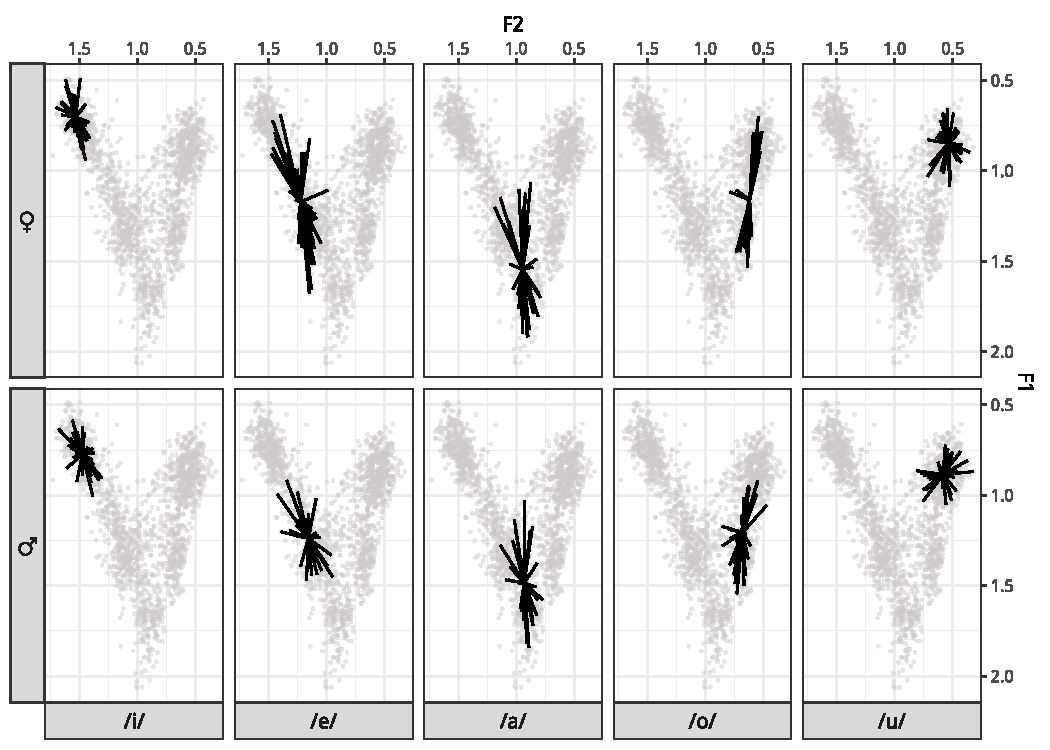
\includegraphics[width=1\linewidth]{91-appendix_brms_files/figure-latex/vowelplot-ref-1} 

}

\caption{Euclidean distances between each observation and the centres of gravity corresponding to each vowel across all participants, by gender (top row: female, bottom row: male) and by vowel (in column), in the normalised F1-F2 plane. The grey background plots represent the individual data collapsed for all individuals (male and female) and all vowels. Note that, for the sake of clarity, this figure represents a unique center of gravity for each vowel for all participants, whereas in the analysis, one center of gravity was used for each vowel and each participant.}\label{fig:vowelplot-ref}
\end{figure}

Then, for each vowel and participant, we computed the Euclidean distance between each observation and the centre of gravity of the whole set of observations in the F1-F2 plane for that participant and that vowel. The data obtained by this process are illustrated in Figure \ref{fig:vowelplot-ref}, and a sample of the final dataset can be found in Table \ref{tab:datavis}.

\begin{table}[H]
\begin{center}
\begin{threeparttable}
\caption{\label{tab:datavis}Ten randomly picked rows from the data.}
\small{
\begin{tabular}{ccccccccc}
\toprule
subj & \multicolumn{1}{c}{gender} & \multicolumn{1}{c}{vowel} & \multicolumn{1}{c}{f1} & \multicolumn{1}{c}{f2} & \multicolumn{1}{c}{f1norm} & \multicolumn{1}{c}{f2norm} & \multicolumn{1}{c}{distance} & \multicolumn{1}{c}{repetition}\\
\midrule
F08 & f & /a/ & 985 & 1509 & 1.758 & 0.840 & 0.226 & 11\\
M02 & m & /o/ & 459 & 906 & 0.982 & 0.585 & 0.230 & 2\\
F04 & f & /a/ & 944 & 1598 & 1.745 & 0.909 & 0.272 & 40\\
F08 & f & /o/ & 725 & 1077 & 1.294 & 0.600 & 0.194 & 28\\
M04 & m & /u/ & 395 & 1307 & 0.938 & 0.865 & 0.286 & 15\\
M02 & m & /a/ & 489 & 1485 & 1.046 & 0.959 & 0.430 & 8\\
M02 & m & /u/ & 374 & 947 & 0.800 & 0.611 & 0.064 & 2\\
F09 & f & /e/ & 422 & 2223 & 0.851 & 1.339 & 0.302 & 4\\
F04 & f & /u/ & 461 & 677 & 0.852 & 0.385 & 0.156 & 7\\
M04 & m & /i/ & 303 & 2241 & 0.720 & 1.483 & 0.101 & 20\\
\bottomrule
\end{tabular}
}
\end{threeparttable}
\end{center}
\end{table}

\hypertarget{constant-effect-of-gender-on-vowel-production-variability}{%
\subsection{Constant effect of gender on vowel production variability}\label{constant-effect-of-gender-on-vowel-production-variability}}

We then built a first model with constant effects only and vague priors on \(\alpha\) and \(\beta\), the intercept and the slope. We contrast-coded \texttt{gender} (f = -0.5, m = 0.5). Our dependent variable was therefore the distance from each individual vowel centre of gravity, which we will refer to as \emph{formant distance} in the following. The formal model can be expressed as:

\[
\begin{aligned}
\text{distance}_{i} &\sim \mathrm{Normal}(\mu_{i}, \sigma_{e}) \\
\mu_{i} &= \alpha + \beta \times \text{gender}_{i} \\
\alpha &\sim \mathrm{Normal}(0, 10) \\
\beta &\sim \mathrm{Normal}(0, 10) \\
\sigma_{e} &\sim \mathrm{HalfCauchy}(10) \\
\end{aligned}
\]

\vspace{5mm}

where the first two lines of the model describe the likelihood and the linear model\footnote{Note that --for the sake of simplicity-- throughout this tutorial we use a Normal likelihood, but other (better) alternatives would include using skew-normal or log-normal models, which are implemented in \texttt{brms} with the \texttt{skew\_normal} and \texttt{lognormal} families. We provide examples in the \protect\hyperlink{suppApp}{supplementary materials}.}. The next three lines define the prior distribution for each parameter of the model, where \(\alpha\) and \(\beta\) are given a vague (weakly informative) Gaussian prior centered on \(0\), and the residual variation is given a Half-Cauchy prior (Gelman, \protect\hyperlink{ref-gelman_prior_2006}{2006}; Polson \& Scott, \protect\hyperlink{ref-polson_half-cauchy_2012}{2012}), thus restricting the range of possible values to positive ones. As depicted in Figure \ref{fig:priorsbmod1}, the \(\mathrm{Normal}(0,10)\) prior is weakly informative in the sense that it grants a relative high weight to \(\alpha\) and \(\beta\) values, between -25 and 25. This corresponds to very large (given the scale of our data) values for, respectively, the mean distance value \(\alpha\), and the mean difference between males and females \(\beta\). The \(\mathrm{HalfCauchy}(10)\) prior placed on \(\sigma_{e}\) also allows very large values of \(\sigma_{e}\), as represented in the right panel of Figure \ref{fig:priorsbmod1}.

\begin{figure}[H]

{\centering 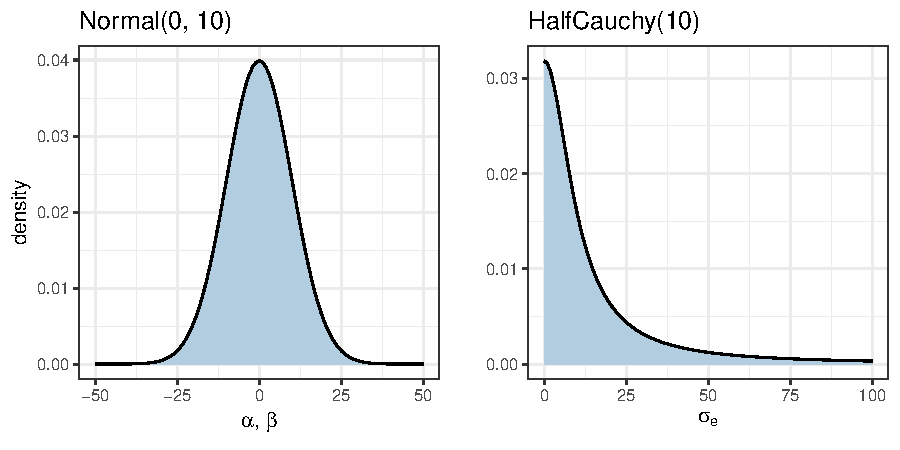
\includegraphics[width=1\linewidth]{91-appendix_brms_files/figure-latex/priorsbmod1-1} 

}

\caption{Prior distributions used in the first model, for $\alpha$ and $\beta$ (left panel) and for the residual variation $\sigma_{e}$ (right panel).}\label{fig:priorsbmod1}
\end{figure}

These priors can be specified in numerous ways (see \texttt{?set\_prior} for more details), among which the following:

\begin{Shaded}
\begin{Highlighting}[]
\NormalTok{prior1 <-}\StringTok{ }\KeywordTok{c}\NormalTok{(}
    \KeywordTok{prior}\NormalTok{(}\KeywordTok{normal}\NormalTok{(}\DecValTok{0}\NormalTok{, }\DecValTok{10}\NormalTok{), }\DataTypeTok{class =}\NormalTok{ Intercept),}
    \KeywordTok{prior}\NormalTok{(}\KeywordTok{normal}\NormalTok{(}\DecValTok{0}\NormalTok{, }\DecValTok{10}\NormalTok{), }\DataTypeTok{class =}\NormalTok{ b, }\DataTypeTok{coef =}\NormalTok{ gender),}
    \KeywordTok{prior}\NormalTok{(}\KeywordTok{cauchy}\NormalTok{(}\DecValTok{0}\NormalTok{, }\DecValTok{10}\NormalTok{), }\DataTypeTok{class =}\NormalTok{ sigma)}
\NormalTok{    )}
\end{Highlighting}
\end{Shaded}

where a prior can be defined over a class of parameters (e.g., for all variance components, using the \texttt{sd} class) or for a specific one, for instance as above by specifying the coefficient (\texttt{coef}) to which the prior corresponds (here the slope of the constant effect of gender).

The model can be fitted with \texttt{brms} with the following command:

\begin{Shaded}
\begin{Highlighting}[]
\KeywordTok{library}\NormalTok{(brms)}

\NormalTok{bmod1 <-}\StringTok{ }\KeywordTok{brm}\NormalTok{(}
\NormalTok{        distance }\OperatorTok{~}\StringTok{ }\NormalTok{gender,}
        \DataTypeTok{data =}\NormalTok{ indo, }\DataTypeTok{family =} \KeywordTok{gaussian}\NormalTok{(),}
        \DataTypeTok{prior =}\NormalTok{ prior1,}
        \DataTypeTok{warmup =} \DecValTok{2000}\NormalTok{, }\DataTypeTok{iter =} \DecValTok{5000}
\NormalTok{    )}
\end{Highlighting}
\end{Shaded}

where \texttt{distance} is the distance from the centre of gravity. The \texttt{iter} argument serves to specify the total number of iterations of the Markov Chain Monte Carlo (MCMC) algorithm, and the \texttt{warmup} argument specifies the number of iterations that are run at the beginning of the process to \enquote{calibrate} the MCMC, so that only \texttt{iter\ -\ warmup} iterations are retained in the end to approximate the shape of the posterior distribution (for more details, see McElreath, \protect\hyperlink{ref-mcelreath_statistical_2016}{2016}\protect\hyperlink{ref-mcelreath_statistical_2016}{b}).

Figure \ref{fig:plotbmod1} depicts the estimations of this first model for the intercept \(\alpha\), the slope \(\beta\), and the residual standard deviation \(\sigma_{e}\). The left part of the plot shows histograms of draws taken from the posterior distribution, and from which several summaries can be computed (e.g., mean, mode, quantiles). The right part of Figure \ref{fig:plotbmod1} shows the behaviour of the two simulations (i.e., the two chains) used to approximate the posterior distribution, where the x-axis represents the number of iterations and the y-axis the value of the parameter. This plot reveals one important aspect of the simulations that should be checked, known as \emph{mixing}. A chain is considered well mixed if it explores many different values for the target parameters and does not stay in the same region of the parameter space. This feature can be evaluated by checking that these plots, usually referred to as \emph{trace plots}, show random scatter around a mean value (they look like a \enquote{fat hairy caterpillar}).

\begin{Shaded}
\begin{Highlighting}[]
\KeywordTok{library}\NormalTok{(tidyverse)}

\NormalTok{bmod1 }\OperatorTok
\StringTok{    }\KeywordTok{plot}\NormalTok{(}
        \DataTypeTok{combo =} \KeywordTok{c}\NormalTok{(}\StringTok{"hist"}\NormalTok{, }\StringTok{"trace"}\NormalTok{), }\DataTypeTok{widths =} \KeywordTok{c}\NormalTok{(}\DecValTok{1}\NormalTok{, }\FloatTok{1.5}\NormalTok{),}
        \DataTypeTok{theme =} \KeywordTok{theme_bw}\NormalTok{(}\DataTypeTok{base_size =} \DecValTok{10}\NormalTok{)}
\NormalTok{        )}
\end{Highlighting}
\end{Shaded}

\begin{figure}[H]

{\centering 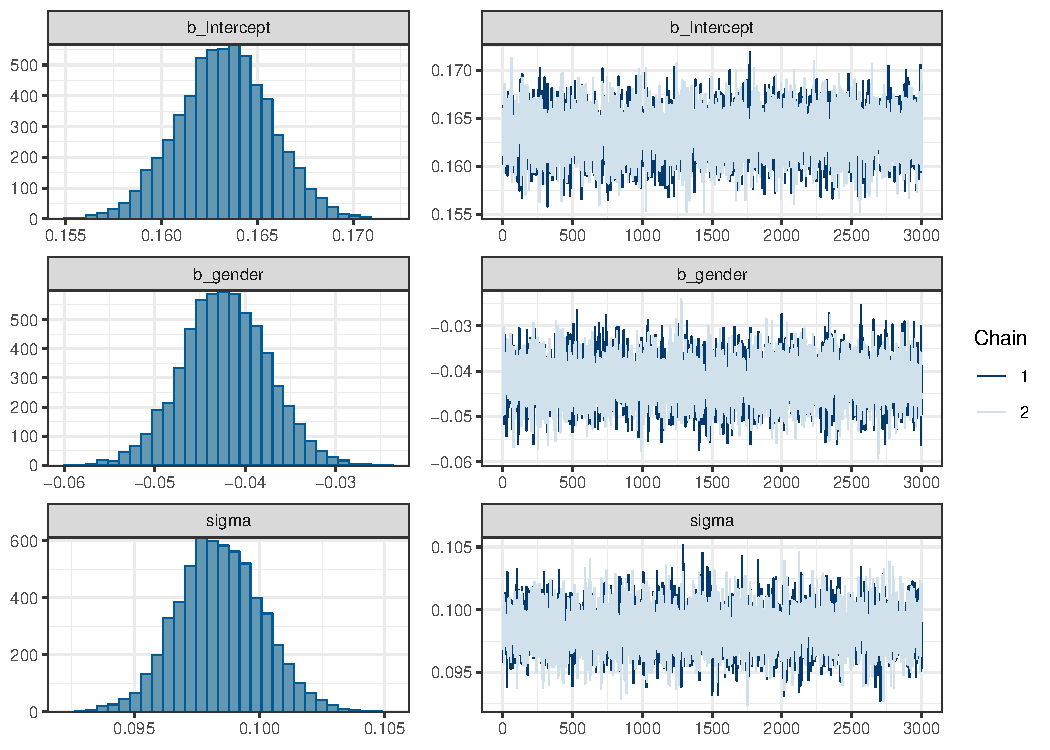
\includegraphics[width=1\linewidth]{91-appendix_brms_files/figure-latex/plotbmod1-1} 

}

\caption{Histograms of posterior samples and trace plots of the intercept, the slope for gender and the standard deviation of the residuals of the constant effects model.}\label{fig:plotbmod1}
\end{figure}

The estimations obtained for this first model are summarised in Table \ref{tab:sumbmod1}, which includes the mean, the standard error (SE), and the lower and upper bounds of the 95\% credible interval (CrI)\footnote{Where a credible interval is the Bayesian analogue of a classical confidence interval, except that probability statements can be made based upon it (e.g., \enquote{given the data and our prior assumptions, there is a 0.95 probability that this interval encompasses the population value \(\theta\)}).} of the posterior distribution for each parameter. As \texttt{gender} was contrast-coded before the analysis (f = -0.5, m = 0.5), the intercept \(\alpha\) corresponds to the grand mean of the formant distance over all participants and has its mean around 0.1633377. The estimate of the slope (\(\beta =\) -0.0422273) suggests that females are more variable than males in the way they pronounce vowels, while the 95\% CrI can be interpreted in a way that there is a \(0.95\) probability that the value of the intercept lies in the {[}-0.0513364, -0.0330469{]} interval.

\begin{table}[H]
\begin{center}
\begin{threeparttable}
\caption{\label{tab:sumbmod1}Posterior mean, standard error, 95\% credible interval and $\hat{R}$
    statistic for each parameter of the constant effect model bmod1.}
\small{
\begin{tabular}{cccccc}
\toprule
parameter & \multicolumn{1}{c}{mean} & \multicolumn{1}{c}{SE} & \multicolumn{1}{c}{lower bound} & \multicolumn{1}{c}{upper bound} & \multicolumn{1}{c}{Rhat}\\
\midrule
$\alpha$ & 0.163 & 0.002 & 0.159 & 0.168 & 1.000\\
$\beta$ & -0.042 & 0.005 & -0.051 & -0.033 & 1.000\\
$\sigma_{e}$ & 0.098 & 0.002 & 0.095 & 0.102 & 1.000\\
\bottomrule
\end{tabular}
}
\end{threeparttable}
\end{center}
\end{table}

The \texttt{Rhat} value corresponds to the \emph{potential scale reduction factor} \(\hat{R}\) (Gelman \& Rubin, \protect\hyperlink{ref-gelman_inference_1992}{1992}), that provides information about the convergence of the algorithm. This index can be conceived as equivalent to the F-ratio in ANOVA. It compares the between-chains variability (i.e., the extent to which different chains differ one from each other) to the within-chain variability (i.e., how widely a chain explores the parameter space), and, as such, gives an index of the convergence of the chains. An overly large between-chains variance (as compared to the within-chain variability) would be a sign that chain-specific characteristics, like the starting value of the algorithm, have a strong influence on the final result. Ideally, the value of \texttt{Rhat} should be close to 1, and should not exceed 1.1. Otherwise, one might consider running more iterations or defining stronger priors (Bürkner, \protect\hyperlink{ref-R-brms}{2018}; Gelman et al., \protect\hyperlink{ref-gelman_bayesian_2013}{2013}).

\hypertarget{shrink}{%
\subsection{Varying intercept model}\label{shrink}}

The first model can be improved by taking into account the dependency between vowel formant measures for each participant. This is handled in MLMs by specifying unique intercepts \(\alpha_{subject[i]}\) and by assigning them a common prior distribution. This strategy corresponds to the following by-subject varying-intercept model, \texttt{bmod2}:

\[
\begin{aligned}
\text{distance}_{i} &\sim \mathrm{Normal}(\mu_{i}, \sigma_{e}) \\
\mu_{i} &= \alpha + \alpha_{subject[i]} + \beta \times \text{gender}_{i} \\
\alpha_{subject} &\sim \mathrm{Normal}(0, \sigma_{subject}) \\
\alpha &\sim \mathrm{Normal}(0, 10) \\
\beta &\sim \mathrm{Normal}(0, 10) \\
\sigma_{subject} &\sim \mathrm{HalfCauchy}(10) \\
\sigma_{e} &\sim \mathrm{HalfCauchy}(10) \\
\end{aligned}
\]

\vspace{5mm}

This model can be fitted with \texttt{brms} with the following command (where we specify the HalfCauchy prior on \(\sigma_{subject}\) by applying it on parameters of class \texttt{sd}):

\begin{Shaded}
\begin{Highlighting}[]
\NormalTok{prior2 <-}\StringTok{ }\KeywordTok{c}\NormalTok{(}
    \KeywordTok{prior}\NormalTok{(}\KeywordTok{normal}\NormalTok{(}\DecValTok{0}\NormalTok{, }\DecValTok{10}\NormalTok{), }\DataTypeTok{class =}\NormalTok{ Intercept),}
    \KeywordTok{prior}\NormalTok{(}\KeywordTok{normal}\NormalTok{(}\DecValTok{0}\NormalTok{, }\DecValTok{10}\NormalTok{), }\DataTypeTok{class =}\NormalTok{ b, }\DataTypeTok{coef =}\NormalTok{ gender),}
    \KeywordTok{prior}\NormalTok{(}\KeywordTok{cauchy}\NormalTok{(}\DecValTok{0}\NormalTok{, }\DecValTok{10}\NormalTok{), }\DataTypeTok{class =}\NormalTok{ sd),}
    \KeywordTok{prior}\NormalTok{(}\KeywordTok{cauchy}\NormalTok{(}\DecValTok{0}\NormalTok{, }\DecValTok{10}\NormalTok{), }\DataTypeTok{class =}\NormalTok{ sigma)}
\NormalTok{    )}

\NormalTok{bmod2 <-}\StringTok{ }\KeywordTok{brm}\NormalTok{(}
\NormalTok{    distance }\OperatorTok{~}\StringTok{ }\NormalTok{gender }\OperatorTok{+}\StringTok{ }\NormalTok{(}\DecValTok{1}\OperatorTok{|}\NormalTok{subj),}
    \DataTypeTok{data =}\NormalTok{ indo, }\DataTypeTok{family =} \KeywordTok{gaussian}\NormalTok{(),}
    \DataTypeTok{prior =}\NormalTok{ prior2,}
    \DataTypeTok{warmup =} \DecValTok{2000}\NormalTok{, }\DataTypeTok{iter =} \DecValTok{10000}
\NormalTok{    )}
\end{Highlighting}
\end{Shaded}

As described in the first part of the present paper, we now have two sources of variation in the model: the standard deviation of the residuals \(\sigma_{e}\) and the standard deviation of the by-subject varying intercepts \(\sigma_{subject}\). The latter represents the standard deviation of the population of varying intercepts, and is also learned from the data. It means that the estimation of each unique intercept will inform the estimation of the population of intercepts, which, in return, will inform the estimation of the other intercepts. We call this sharing of information between groups the \emph{partial pooling} strategy, in comparison with the \emph{no pooling} strategy, where each intercept is estimated independently, and with the \emph{complete pooling} strategy, in which all intercepts are given the same value (Gelman et al., \protect\hyperlink{ref-gelman_bayesian_2013}{2013}; Gelman \& Hill, \protect\hyperlink{ref-gelman_data_2006}{2006}; McElreath, \protect\hyperlink{ref-mcelreath_statistical_2016}{2016}\protect\hyperlink{ref-mcelreath_statistical_2016}{b}). This is one of the most essential features of MLMs, and what leads to better estimations than single-level regression models for repeated measurements or unbalanced sample sizes. This pooling of information is made apparent through the phenomenon of \emph{shrinkage}, which is illustrated in Figure \ref{fig:ranefplotbmod2}, and later on, in Figure \ref{fig:shrinkageplot}.

Figure \ref{fig:ranefplotbmod2} shows the posterior distribution as estimated by this second model for each participant, in relation to the raw mean of its category (i.e., females or males), represented by the vertical dashed lines. We can see for instance that participants \texttt{M02} and \texttt{F09} have smaller average distance than the means of their groups, while participants \texttt{M03} and \texttt{F08} have larger ones. The arrows represent the amount of \emph{shrinkage}, that is, the deviation between the mean in the raw data (represented by a cross underneath each density) and the estimated mean of the posterior distribution (represented by the peak of the arrow). As shown in Figure \ref{fig:ranefplotbmod2}, this \emph{shrinkage} is always directed toward the mean of the considered group (i.e., females or males) and the amount of \emph{shrinkage} is determined by the deviation of the individual mean from its group mean. This mechanism acts like a safeguard against overfitting, preventing the model from overly trusting each individual datum.

\begin{figure}[H]

{\centering 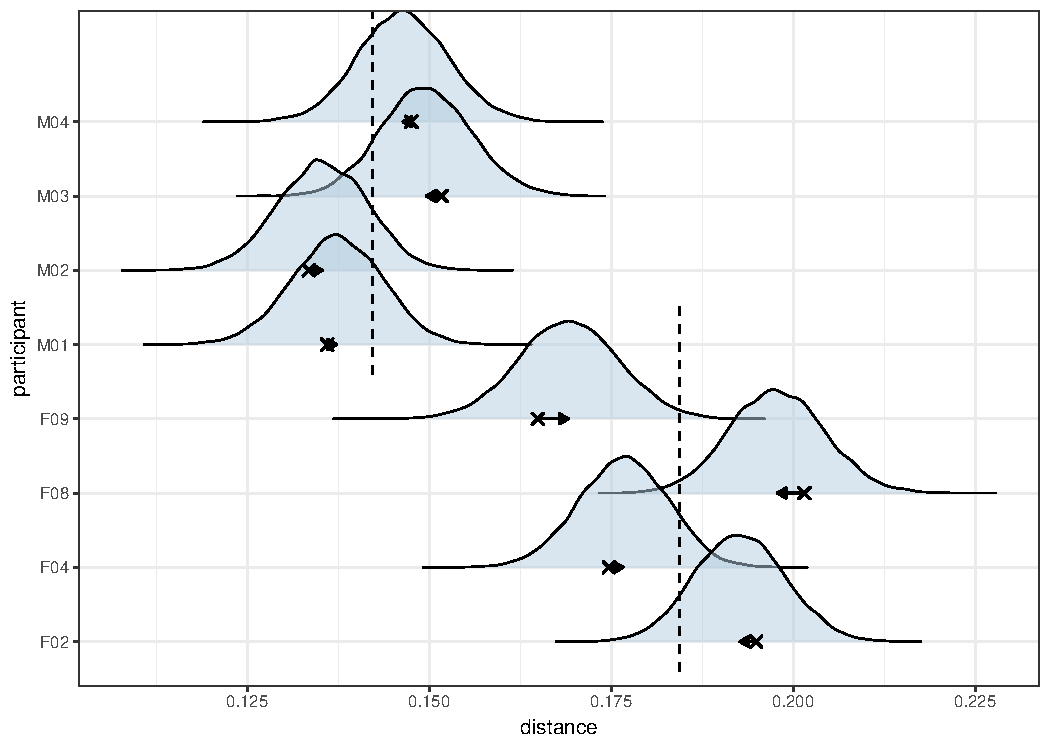
\includegraphics[width=1\linewidth]{91-appendix_brms_files/figure-latex/ranefplotbmod2-1} 

}

\caption{Posterior distributions by subject, as estimated by the `bmod2` model. The vertical dashed lines represent the means of the formant distances for the female and male groups. Crosses represent the mean of the raw data, for each participant. Arrows represent the amount of shrinkage, between the raw mean and the estimation of the model (the mean of the posterior distribution).}\label{fig:ranefplotbmod2}
\end{figure}

The marginal posterior distribution of each parameter obtained with \texttt{bmod2} is summarised in Table \ref{tab:sumbmod2}, where the \texttt{Rhat} values close to \(1\) suggest that the model has converged. We see that the estimates of \(\alpha\) and \(\beta\) are similar to the estimates of the first model, except that the SE is now slightly larger. This result might seem surprising at first sight, as we expected to improve the first model by adding a by-subject varying intercept. In fact, it reveals an underestimation of the SE when using the first model. Indeed, the first model assumes independence of observations, which is violated in our case. This highlights the general need for careful consideration of the model's assumptions when interpreting its estimations. The first model seemingly gives highly certain estimates, but these estimations are only valid in the \enquote{independence of observations} world (see also the distinction between the \emph{small world} and the \emph{large world} in McElreath, \protect\hyperlink{ref-mcelreath_statistical_2016}{2016}\protect\hyperlink{ref-mcelreath_statistical_2016}{b}). Moreover, estimating an intercept by subject (as in the second model) increases the precision of estimation, but it also makes the average estimation less certain, thus resulting in a larger SE.

\begin{table}[H]
\begin{center}
\begin{threeparttable}
\caption{\label{tab:sumbmod2}Posterior mean, standard error, 95\% credible interval and $\hat{R}$
    statistic for each parameter of model bmod2 with a varying intercept by subject.}
\small{
\begin{tabular}{cccccc}
\toprule
parameter & \multicolumn{1}{c}{mean} & \multicolumn{1}{c}{SE} & \multicolumn{1}{c}{lower bound} & \multicolumn{1}{c}{upper bound} & \multicolumn{1}{c}{Rhat}\\
\midrule
$\alpha$ & 0.163 & 0.007 & 0.150 & 0.176 & 1.000\\
$\beta$ & -0.042 & 0.013 & -0.069 & -0.016 & 1.000\\
$\sigma_{subject}$ & 0.016 & 0.008 & 0.006 & 0.035 & 1.000\\
$\sigma_{e}$ & 0.098 & 0.002 & 0.095 & 0.101 & 1.000\\
\bottomrule
\end{tabular}
}
\end{threeparttable}
\end{center}
\end{table}

This model (\texttt{bmod2}), however, is still not adequate to describe the data, as the dependency between repetitions of each vowel is not taken into account. In \texttt{bmod3}, we added a by-vowel varying intercept, thus also allowing each vowel to have a different general level of variability.

\[
\begin{aligned}
\text{distance}_{i} &\sim \mathrm{Normal}(\mu_{i}, \sigma_{e}) \\
\mu_{i} &= \alpha + \alpha_{subject[i]} + \alpha_{vowel[i]} + \beta \times \text{gender}_{i} \\
\alpha_{subj} &\sim \mathrm{Normal}(0, \sigma_{subject}) \\
\alpha_{vowel} &\sim \mathrm{Normal}(0, \sigma_{vowel}) \\
\alpha &\sim \mathrm{Normal}(0, 10) \\
\beta &\sim \mathrm{Normal}(0, 10) \\
\sigma_{e} &\sim \mathrm{HalfCauchy}(10) \\
\sigma_{subject} &\sim \mathrm{HalfCauchy}(10) \\
\sigma_{vowel} &\sim \mathrm{HalfCauchy}(10) \\
\end{aligned}
\]

\vspace{5mm}

This model can be fitted with \texttt{brms} with the following command:

\begin{Shaded}
\begin{Highlighting}[]
\NormalTok{prior3 <-}\StringTok{ }\KeywordTok{c}\NormalTok{(}
    \KeywordTok{prior}\NormalTok{(}\KeywordTok{normal}\NormalTok{(}\DecValTok{0}\NormalTok{, }\DecValTok{10}\NormalTok{), }\DataTypeTok{class =}\NormalTok{ Intercept),}
    \KeywordTok{prior}\NormalTok{(}\KeywordTok{normal}\NormalTok{(}\DecValTok{0}\NormalTok{, }\DecValTok{10}\NormalTok{), }\DataTypeTok{class =}\NormalTok{ b, }\DataTypeTok{coef =}\NormalTok{ gender),}
    \KeywordTok{prior}\NormalTok{(}\KeywordTok{cauchy}\NormalTok{(}\DecValTok{0}\NormalTok{, }\DecValTok{10}\NormalTok{), }\DataTypeTok{class =}\NormalTok{ sd),}
    \KeywordTok{prior}\NormalTok{(}\KeywordTok{cauchy}\NormalTok{(}\DecValTok{0}\NormalTok{, }\DecValTok{10}\NormalTok{), }\DataTypeTok{class =}\NormalTok{ sigma)}
\NormalTok{    )}

\NormalTok{bmod3 <-}\StringTok{ }\KeywordTok{brm}\NormalTok{(}
\NormalTok{    distance }\OperatorTok{~}\StringTok{ }\NormalTok{gender }\OperatorTok{+}\StringTok{ }\NormalTok{(}\DecValTok{1}\OperatorTok{|}\NormalTok{subj) }\OperatorTok{+}\StringTok{ }\NormalTok{(}\DecValTok{1}\OperatorTok{|}\NormalTok{vowel),}
    \DataTypeTok{data =}\NormalTok{ indo, }\DataTypeTok{family =} \KeywordTok{gaussian}\NormalTok{(),}
    \DataTypeTok{prior =}\NormalTok{ prior3,}
    \DataTypeTok{warmup =} \DecValTok{2000}\NormalTok{, }\DataTypeTok{iter =} \DecValTok{10000}
\NormalTok{    )}
\end{Highlighting}
\end{Shaded}

where the same Half-Cauchy is specified for the two varying intercepts, by applying it directly to the \texttt{sd} class.

\begin{table}[H]
\begin{center}
\begin{threeparttable}
\caption{\label{tab:sumbmod3}Posterior mean, standard error, 95\% credible interval and $\hat{R}$
    statistic for each parameter of model bmod3 with a varying intercept by subject and by vowel.}
\small{
\begin{tabular}{cccccc}
\toprule
parameter & \multicolumn{1}{c}{mean} & \multicolumn{1}{c}{SE} & \multicolumn{1}{c}{lower bound} & \multicolumn{1}{c}{upper bound} & \multicolumn{1}{c}{Rhat}\\
\midrule
$\alpha$ & 0.164 & 0.041 & 0.087 & 0.246 & 1.000\\
$\beta$ & -0.042 & 0.014 & -0.069 & -0.015 & 1.000\\
$\sigma_{subject}$ & 0.016 & 0.008 & 0.007 & 0.036 & 1.001\\
$\sigma_{vowel}$ & 0.075 & 0.051 & 0.031 & 0.200 & 1.002\\
$\sigma_{e}$ & 0.088 & 0.002 & 0.085 & 0.091 & 1.000\\
\bottomrule
\end{tabular}
}
\end{threeparttable}
\end{center}
\end{table}

The marginal posterior distribution of each parameter is summarised in Table \ref{tab:sumbmod3}. We can compute the intra-class correlation (ICC, see section \ref{MLM}) to estimate the relative variability associated with each varying effect: \(ICC_{subject}\) is equal to 0.0339265 and \(ICC_{vowel}\) is equal to 0.4232396. The rather high ICC for vowels suggests that observations are highly correlated within each vowel, thus stressing the relevance of allocating a unique intercept by vowel\footnote{But please note that we do not mean to suggest that the varying intercept for subjects should be removed because its ICC is low.}.

\hypertarget{including-a-correlation-between-varying-intercept-and-varying-slope}{%
\subsection{Including a correlation between varying intercept and varying slope}\label{including-a-correlation-between-varying-intercept-and-varying-slope}}

One can legitimately question the assumption that the differences between male and female productions are identical for each vowel. To explore this issue, we thus added a varying slope for the effect of gender, allowing it to vary by vowel. Moreover, we can exploit the correlation between the baseline level of variability by vowel, and the amplitude of the difference between males and females in pronouncing them. For instance, we can observe that the pronunciation of /a/ is more variable in general. We might want to know whether females tend to pronounce vowels that are situated at a specific location in the F1-F2 plane with less variability than males. In other words, we might be interested in knowing whether the effect of \texttt{gender} is correlated with the baseline level of variability. This is equivalent to investigating the \emph{dependency}, or the correlation between the varying intercepts and the varying slopes. We thus estimated this correlation by modelling \(\alpha_{vowel}\) and \(\beta_{vowel}\) as issued from the same multivariate normal distribution (a multivariate normal distribution is a generalisation of the usual normal distribution to more than one dimension), centered on \(0\) and with some covariance matrix \(\textbf{S}\), as specified on the third line of the following model:

\[
\begin{aligned}
\text{distance}_{i} &\sim \mathrm{Normal}(\mu_{i}, \sigma_{e}) \\
\mu_{i} &= \alpha + \alpha_{subject[i]} + \alpha_{vowel[i]} + (\beta + \beta_{vowel[i]}) \times \text{gender}_{i} \\
\begin{bmatrix}
\alpha_{\text{vowel}} \\
\beta_{\text{vowel}} \\
\end{bmatrix}
&\sim \mathrm{MVNormal}\bigg(\begin{bmatrix} 0 \\ 0 \end{bmatrix}, \textbf{S}\bigg) \\
\textbf{S} &=
\begin{pmatrix}
\sigma_{\alpha_{vowel}}^{2} & \sigma_{\alpha_{vowel}}\sigma_{\beta{vowel}} \rho \\
\sigma_{\alpha_{vowel}}\sigma_{\beta{vowel}} \rho & \sigma_{\beta_{vowel}}^{2} \\
\end{pmatrix} \\
\alpha_{subject} &\sim \mathrm{Normal}(0, \sigma_{subject}) \\
\alpha &\sim \mathrm{Normal}(0, 10) \\
\beta &\sim \mathrm{Normal}(0, 10) \\
\sigma_{e} &\sim \mathrm{HalfCauchy}(10) \\
\sigma_{\alpha_{vowel}} &\sim \mathrm{HalfCauchy}(10) \\
\sigma_{\beta_{vowel}} &\sim \mathrm{HalfCauchy}(10) \\
\sigma_{subject} &\sim \mathrm{HalfCauchy}(10) \\
\textbf{R} &\sim \mathrm{LKJcorr}(2) \\
\end{aligned}
\]

\vspace{5mm}

where \(\textbf{R}\) is the correlation matrix \(\textbf{R} = \begin{pmatrix} 1 & \rho \\ \rho & 1 \end{pmatrix}\) and \(\rho\) is the correlation between intercepts and slopes, used in the computation of \(\textbf{S}\). This matrix is given the LKJ-Correlation prior (Lewandowski, Kurowicka, \& Joe, \protect\hyperlink{ref-lewandowski_generating_2009}{2009}) with a parameter \(\zeta\) (zeta) that controls the strength of the correlation\footnote{The LKJ prior is the default prior for correlation matrices in \texttt{brms}.}. When \(\zeta = 1\), the prior distribution on the correlation is uniform between \(-1\) and \(1\). When \(\zeta > 1\), the prior distribution is peaked around a zero correlation, while lower values of \(\zeta\) (\(0 < \zeta < 1\)) allocate more weight to extreme values (i.e., close to -1 and 1) of \(\rho\) (see Figure \ref{fig:lkj}).

\begin{figure}[H]

{\centering 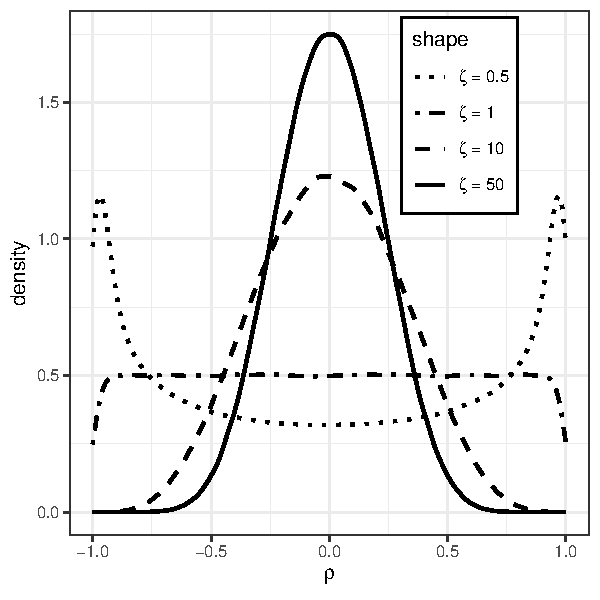
\includegraphics[width=1\linewidth]{91-appendix_brms_files/figure-latex/lkj-1} 

}

\caption{Visualisation of the LKJ prior for different values of the shape parameter $\zeta$.}\label{fig:lkj}
\end{figure}

\begin{Shaded}
\begin{Highlighting}[]
\NormalTok{prior4 <-}\StringTok{ }\KeywordTok{c}\NormalTok{(}
    \KeywordTok{prior}\NormalTok{(}\KeywordTok{normal}\NormalTok{(}\DecValTok{0}\NormalTok{, }\DecValTok{10}\NormalTok{), }\DataTypeTok{class =}\NormalTok{ Intercept),}
    \KeywordTok{prior}\NormalTok{(}\KeywordTok{normal}\NormalTok{(}\DecValTok{0}\NormalTok{, }\DecValTok{10}\NormalTok{), }\DataTypeTok{class =}\NormalTok{ b, }\DataTypeTok{coef =}\NormalTok{ gender),}
    \KeywordTok{prior}\NormalTok{(}\KeywordTok{cauchy}\NormalTok{(}\DecValTok{0}\NormalTok{, }\DecValTok{10}\NormalTok{), }\DataTypeTok{class =}\NormalTok{ sd),}
    \KeywordTok{prior}\NormalTok{(}\KeywordTok{cauchy}\NormalTok{(}\DecValTok{0}\NormalTok{, }\DecValTok{10}\NormalTok{), }\DataTypeTok{class =}\NormalTok{ sigma),}
    \KeywordTok{prior}\NormalTok{(}\KeywordTok{lkj}\NormalTok{(}\DecValTok{2}\NormalTok{), }\DataTypeTok{class =}\NormalTok{ cor)}
\NormalTok{    )}

\NormalTok{bmod4 <-}\StringTok{ }\KeywordTok{brm}\NormalTok{(}
\NormalTok{    distance }\OperatorTok{~}\StringTok{ }\NormalTok{gender }\OperatorTok{+}\StringTok{ }\NormalTok{(}\DecValTok{1}\OperatorTok{|}\NormalTok{subj) }\OperatorTok{+}\StringTok{ }\NormalTok{(}\DecValTok{1} \OperatorTok{+}\StringTok{ }\NormalTok{gender}\OperatorTok{|}\NormalTok{vowel),}
    \DataTypeTok{data =}\NormalTok{ indo, }\DataTypeTok{family =} \KeywordTok{gaussian}\NormalTok{(),}
    \DataTypeTok{prior =}\NormalTok{ prior4,}
    \DataTypeTok{warmup =} \DecValTok{2000}\NormalTok{, }\DataTypeTok{iter =} \DecValTok{10000}
\NormalTok{    )}
\end{Highlighting}
\end{Shaded}

Estimates of this model are summarised in Table \ref{tab:sumbmod4}. This summary reveals a negative correlation between the intercepts and slopes for vowels, meaning that vowels with a large \enquote{baseline level of variability} (i.e., with a large average \texttt{distance} value) tend to be pronounced with more variability by females than by males. However, we notice that this model's estimation of \(\beta\) is even more uncertain than that of the previous models, as shown by the associated standard error and the width of the credible interval.

\begin{table}[H]
\begin{center}
\begin{threeparttable}
\caption{\label{tab:sumbmod4}Posterior mean, standard error, 95\% credible interval and $\hat{R}$
    statistic for each parameter of model bmod4 with a varying intercept and varying slope by vowel.}
\small{
\begin{tabular}{cccccc}
\toprule
parameter & \multicolumn{1}{c}{mean} & \multicolumn{1}{c}{SE} & \multicolumn{1}{c}{lower bound} & \multicolumn{1}{c}{upper bound} & \multicolumn{1}{c}{Rhat}\\
\midrule
$\alpha$ & 0.163 & 0.034 & 0.094 & 0.231 & 1.000\\
$\beta$ & -0.042 & 0.031 & -0.101 & 0.018 & 1.000\\
$\sigma_{subject}$ & 0.016 & 0.008 & 0.007 & 0.036 & 1.000\\
$\sigma_{\alpha_{vowel}}$ & 0.067 & 0.041 & 0.029 & 0.165 & 1.000\\
$\sigma_{\beta_{vowel}}$ & 0.053 & 0.034 & 0.022 & 0.139 & 1.000\\
$\rho$ & -0.494 & 0.354 & -0.952 & 0.366 & 1.000\\
$\sigma_{e}$ & 0.086 & 0.001 & 0.084 & 0.089 & 1.000\\
\bottomrule
\end{tabular}
}
\end{threeparttable}
\end{center}
\end{table}

Figure \ref{fig:shrinkageplot} illustrates the negative correlation between the by-vowel intercepts and the by-vowel slopes, meaning that vowels that tend to have higher \enquote{baseline variability} (i.e., /e/, /o/, /a/), tend to show a stronger effect of \texttt{gender}. This figure also illustrates the amount of shrinkage, here in the parameter space. We can see that the \emph{partial pooling} estimate is shrunk somewhere between the \emph{no pooling} estimate and the \emph{complete pooling} estimate (i.e., the grand mean). This illustrates again the mechanism by which MLMs balance the risk of overfitting and underfitting (McElreath, \protect\hyperlink{ref-mcelreath_statistical_2016}{2016}\protect\hyperlink{ref-mcelreath_statistical_2016}{b}).

\begin{figure}[H]

{\centering \includegraphics[width=1\linewidth]{91-appendix_brms_files/figure-latex/shrinkageplot-1} 

}

\caption{Shrinkage of estimates in the parameter space, due to the pooling of information between clusters (based on the `bmod4` model). The ellipses represent the contours of the bivariate distribution, at different degrees of confidence 0.1, 0.3, 0.5 and 0.7.}\label{fig:shrinkageplot}
\end{figure}

\hypertarget{varying-intercept-and-varying-slope-model-interaction-between-subject-and-vowel}{%
\subsection{Varying intercept and varying slope model, interaction between subject and vowel}\label{varying-intercept-and-varying-slope-model-interaction-between-subject-and-vowel}}

So far, we modelled varying effects of subjects and vowels. In this study, these varying factors were crossed, meaning that every subject had to pronounce every vowel. Let us now imagine a situation in which Subject 4 systematically mispronounced the /i/ vowel. This would be a source of systematic variation over replicates which is not considered in the model (\texttt{bmod4}), because this model can only adjust parameters for either vowel or participant, but not for a specific vowel for a specific participant.

In building the next model, we added a varying intercept for the interaction between subject and vowel, that is, we created an index variable that allocates a unique value at each crossing of the two variables (e.g., Subject1-vowel/a/, Subject1-vowel/i/, etc.), resulting in \(8 \times 5 = 40\) intercepts to be estimated (for a review of multilevel modeling in various experimental designs, see Judd, Westfall, \& Kenny, \protect\hyperlink{ref-judd_experiments_2017}{2017}). This varying intercept for the interaction between subject and vowel represents the systematic variation associated with a specific subject pronouncing a specific vowel. This model can be written as follows, for any observation \(i\):

\[
\begin{aligned}
\text{distance}_{i} &\sim \mathrm{Normal}(\mu_{i}, \sigma_{e}) \\
\mu_{i} &= \alpha + \alpha_{subject[i]} + \alpha_{vowel[i]} + \alpha_{subject:vowel[i]} + (\beta + \beta_{vowel[i]}) \times \text{gender}_{i} \\
\begin{bmatrix}
\alpha_{\text{vowel}} \\
\beta_{\text{vowel}} \\
\end{bmatrix}
&\sim \mathrm{MVNormal}\bigg(\begin{bmatrix} 0 \\ 0 \end{bmatrix}, \textbf{S}\bigg) \\
\textbf{S} &=
\begin{pmatrix}
\sigma_{\alpha_{vowel}}^{2} & \sigma_{\alpha_{vowel}}\sigma_{\beta{vowel}} \rho \\
\sigma_{\alpha_{vowel}}\sigma_{\beta{vowel}} \rho & \sigma_{\beta_{vowel}}^{2} \\
\end{pmatrix} \\
\alpha_{subject} &\sim \mathrm{Normal}(0, \sigma_{subject}) \\
\alpha_{subject:vowel} &\sim \mathrm{Normal}(0, \sigma_{subject:vowel}) \\
\alpha &\sim \mathrm{Normal}(0, 10) \\
\beta &\sim \mathrm{Normal}(0, 10) \\
\sigma_{e} &\sim \mathrm{HalfCauchy}(10) \\
\sigma_{subject} &\sim \mathrm{HalfCauchy}(10) \\
\sigma_{subject:vowel} &\sim \mathrm{HalfCauchy}(10) \\
\sigma_{\alpha_{vowel}} &\sim \mathrm{HalfCauchy}(10) \\
\sigma_{\beta_{vowel}} &\sim \mathrm{HalfCauchy}(10) \\
\textbf{R} &\sim \mathrm{LKJcorr}(2) \\
\end{aligned}
\]
\vspace{5mm}

This model can be fitted with the following command:

\begin{Shaded}
\begin{Highlighting}[]
\NormalTok{prior5 <-}\StringTok{ }\KeywordTok{c}\NormalTok{(}
    \KeywordTok{prior}\NormalTok{(}\KeywordTok{normal}\NormalTok{(}\DecValTok{0}\NormalTok{, }\DecValTok{10}\NormalTok{), }\DataTypeTok{class =}\NormalTok{ Intercept),}
    \KeywordTok{prior}\NormalTok{(}\KeywordTok{normal}\NormalTok{(}\DecValTok{0}\NormalTok{, }\DecValTok{10}\NormalTok{), }\DataTypeTok{class =}\NormalTok{ b, }\DataTypeTok{coef =}\NormalTok{ gender),}
    \KeywordTok{prior}\NormalTok{(}\KeywordTok{cauchy}\NormalTok{(}\DecValTok{0}\NormalTok{, }\DecValTok{10}\NormalTok{), }\DataTypeTok{class =}\NormalTok{ sd),}
    \KeywordTok{prior}\NormalTok{(}\KeywordTok{cauchy}\NormalTok{(}\DecValTok{0}\NormalTok{, }\DecValTok{10}\NormalTok{), }\DataTypeTok{class =}\NormalTok{ sigma),}
    \KeywordTok{prior}\NormalTok{(}\KeywordTok{lkj}\NormalTok{(}\DecValTok{2}\NormalTok{), }\DataTypeTok{class =}\NormalTok{ cor)}
\NormalTok{    )}

\NormalTok{bmod5 <-}\StringTok{ }\KeywordTok{brm}\NormalTok{(}
\NormalTok{    distance }\OperatorTok{~}\StringTok{ }\NormalTok{gender }\OperatorTok{+}\StringTok{ }\NormalTok{(}\DecValTok{1}\OperatorTok{|}\NormalTok{subj) }\OperatorTok{+}\StringTok{ }\NormalTok{(}\DecValTok{1} \OperatorTok{+}\StringTok{ }\NormalTok{gender}\OperatorTok{|}\NormalTok{vowel) }\OperatorTok{+}\StringTok{ }\NormalTok{(}\DecValTok{1}\OperatorTok{|}\NormalTok{subj}\OperatorTok{:}\NormalTok{vowel),}
    \DataTypeTok{data =}\NormalTok{ indo, }\DataTypeTok{family =} \KeywordTok{gaussian}\NormalTok{(),}
    \DataTypeTok{prior =}\NormalTok{ prior5,}
    \DataTypeTok{warmup =} \DecValTok{2000}\NormalTok{, }\DataTypeTok{iter =} \DecValTok{10000}
\NormalTok{    )}
\end{Highlighting}
\end{Shaded}

Estimates of this model are summarised in Table \ref{tab:sumbmod5}. From this table, we first notice that the more varying effects we add, the more the model is uncertain about the estimation of \(\alpha\) and \(\beta\), which can be explained in the same way as in section 2.2. Second, we see the opposite pattern for \(\sigma_{e}\), the residuals standard deviation, which has decreased by a considerable amount compared to the first model, indicating a better fit.

\begin{table}[H]
\begin{center}
\begin{threeparttable}
\caption{\label{tab:sumbmod5}Posterior mean, standard error, 95\% credible interval and $\hat{R}$
    statistic for each parameter of model bmod5 with a varying intercept and a
    varying slope by vowel and a varying intercept for the interaction between subject and vowel.}
\small{
\begin{tabular}{cccccc}
\toprule
parameter & \multicolumn{1}{c}{mean} & \multicolumn{1}{c}{SE} & \multicolumn{1}{c}{lower bound} & \multicolumn{1}{c}{upper bound} & \multicolumn{1}{c}{Rhat}\\
\midrule
$\alpha$ & 0.164 & 0.038 & 0.094 & 0.240 & 1.000\\
$\beta$ & -0.043 & 0.033 & -0.104 & 0.018 & 1.001\\
$\sigma_{subject}$ & 0.012 & 0.009 & 0.001 & 0.033 & 1.000\\
$\sigma_{subject:vowel}$ & 0.024 & 0.004 & 0.016 & 0.034 & 1.002\\
$\sigma_{\alpha_{vowel}}$ & 0.069 & 0.044 & 0.029 & 0.180 & 1.001\\
$\sigma_{\beta_{vowel}}$ & 0.051 & 0.038 & 0.013 & 0.144 & 1.000\\
$\rho$ & -0.424 & 0.383 & -0.945 & 0.473 & 1.000\\
$\sigma_{e}$ & 0.085 & 0.001 & 0.082 & 0.088 & 1.000\\
\bottomrule
\end{tabular}
}
\end{threeparttable}
\end{center}
\end{table}

\hypertarget{model-comparison}{%
\section{Model comparison}\label{model-comparison}}

Once we have built a set of models, we need to know which model is the more accurate and should be used to draw conclusions. It might be a little tricky to select the model that has the better absolute fit on the actual data (using for instance \(R^{2}\)), as this model will not necessarily perform as well on new data. Instead, we might want to choose the model that has the best predictive abilities, that is, the model that performs the best when it comes to predicting data that have not yet been observed. We call this ability the out-of-sample predictive performance of the model (McElreath, \protect\hyperlink{ref-mcelreath_statistical_2016}{2016}\protect\hyperlink{ref-mcelreath_statistical_2016}{b}). When additional data is not available, cross-validation techniques can be used to obtain an approximation of the model's predictive abilities, among which the Bayesian leave-one-out-cross-validation (LOO-CV, Vehtari, Gelman, \& Gabry, \protect\hyperlink{ref-vehtari_practical_2017}{2017}). Another useful tool, and asymptotically equivalent to the LOO-CV, is the Watanabe Akaike Information Criterion (WAIC, Watanabe, \protect\hyperlink{ref-watanabe_asymptotic_2010}{2010}), which can be conceived as a generalisation of the Akaike Information Criterion (AIC, Akaike, \protect\hyperlink{ref-akaike_new_1974}{1974})\footnote{More details on model comparison using cross-validation techniques can be found in Nicenboim \& Vasishth (\protect\hyperlink{ref-nicenboim_statistical_2016}{2016}). See also Gelman, Hwang, \& Vehtari (\protect\hyperlink{ref-gelman_understanding_2014}{2014}) for a complete comparison of information criteria.}.

Both WAIC and LOO-CV indexes are easily computed in \texttt{brms} with the \texttt{WAIC} and the \texttt{LOO} functions, where \(n\) models can be compared with the following call: \texttt{LOO(model1,\ model2,\ ...,\ modeln)}. These functions also provide an estimate of the uncertainty associated with these indexes (in the form of a SE), as well as a difference score \(\Delta \text{LOOIC}\), which is computed by taking the difference between each pair of information criteria. A comparison of the five models we fitted can be found in Table \ref{tab:modelcomparison}.

\begin{table}[H]
\begin{center}
\begin{threeparttable}
\caption{\label{tab:modelcomparison}Model comparison with LOOIC.}
\small{
\begin{tabular}{ccccr}
\toprule
Model & \multicolumn{1}{c}{LOOIC} & \multicolumn{1}{c}{SE} & \multicolumn{1}{c}{$\Delta$LOOIC} & \multicolumn{1}{c}{right side of the formula}\\
\midrule
bmod5 & -3590.81 & 68.14 & 0.00 & gender + (1 | subj) + (1 + gender | vowel) + (1 | subj:vowel)\\
bmod4 & -3536.69 & 66.92 & 54.12 & gender + (1 | subj) + (1 + gender | vowel)\\
bmod3 & -3477.13 & 67.17 & 113.68 & gender + (1 | subj) + (1 | vowel)\\
bmod2 & -3114.21 & 65.25 & 476.60 & gender + (1 | subj)\\
bmod1 & -3100.99 & 66.74 & 489.83 & gender\\
\bottomrule
\end{tabular}
}
\end{threeparttable}
\end{center}
\end{table}

We see from Table \ref{tab:modelcomparison} that \texttt{bmod5} (i.e., the last model) is performing much better than the other models, as it has the lower LOOIC. We then based our conclusions (see last section) on the estimations of this model. We also notice that each addition to the initial model brought improvement in terms of predictive accuracy, as the set of models is ordered from the first to the last model. This should not be taken as a general rule though, as successive additions made to an original model could also lead to \emph{overfitting}, corresponding to a situation in which the model is over-specified in regards to the data, which makes the model good to explain the data at hand, but very bad to predict non-observed data. In such cases, information criteria and indexes that rely exclusively on goodness-of-fit (such as \(R^{2}\)) would point to different conclusions.

\hypertarget{comparison-of-brms-and-lme4-estimations}{%
\section{\texorpdfstring{Comparison of \texttt{brms} and \texttt{lme4} estimations}{Comparison of brms and lme4 estimations}}\label{comparison-of-brms-and-lme4-estimations}}

Figure \ref{fig:compestim} illustrates the comparison of \texttt{brms} (Bayesian approach) and \texttt{lme4} (frequentist approach) estimates for the last model (\texttt{bmod5}), fitted in \texttt{lme4} with the following command.

\begin{Shaded}
\begin{Highlighting}[]
\NormalTok{lmer_model <-}\StringTok{ }\KeywordTok{lmer}\NormalTok{(}
\NormalTok{    distance }\OperatorTok{~}\StringTok{ }\NormalTok{gender }\OperatorTok{+}\StringTok{ }\NormalTok{(}\DecValTok{1}\OperatorTok{|}\NormalTok{subj) }\OperatorTok{+}\StringTok{ }\NormalTok{(}\DecValTok{1} \OperatorTok{+}\StringTok{ }\NormalTok{gender}\OperatorTok{|}\NormalTok{vowel) }\OperatorTok{+}\StringTok{ }\NormalTok{(}\DecValTok{1}\OperatorTok{|}\NormalTok{subj}\OperatorTok{:}\NormalTok{vowel),}
    \DataTypeTok{REML =} \OtherTok{FALSE}\NormalTok{, }\DataTypeTok{data =}\NormalTok{ indo}
\NormalTok{    )}
\end{Highlighting}
\end{Shaded}

Densities represent the posterior distribution as estimated by \texttt{brms} along with 95\% credible intervals, while the crosses underneath represent the \emph{maximum likelihood estimate} (MLE) from \texttt{lme4} along with 95\% confidence intervals, obtained with parametric bootstrapping.

\begin{figure}[H]

{\centering \includegraphics[width=1\linewidth]{91-appendix_brms_files/figure-latex/compestim-1} 

}

\caption{Comparison of estimations from `brms` and `lme4`. Dots represent means of posterior distribution along with 95\% CrIs, as estimated by the `bmod5` model. Crosses represent estimations of `lme4` along with bootstrapped 95\% CIs.}\label{fig:compestim}
\end{figure}

We can see that the estimations of \texttt{brms} and \texttt{lme4} are for the most part very similar. The differences we observe for \(\sigma_{\alpha_{vowel}}\) and \(\sigma_{\beta_{vowel}}\) might be explained by the skewness of the posterior distribution. Indeed, in these cases (i.e., when the distribution is not symmetric), the mode of the distribution would better coincide with the \texttt{lme4} estimate. This figure also illustrates a limitation of frequentist MLMs that we discussed in the first part of the current paper. If we look closely at the estimates of \texttt{lme4}, we can notice that the MLE for the correlation \(\rho\) is at its boundary, as \(\rho = -1\). This might be interpreted in (at least) two ways. The first interpretation is what Eager \& Roy (\protect\hyperlink{ref-eager_mixed_2017}{2017}) call the \emph{parsimonious convergence hypothesis} (PCH) and consists in saying that this aberrant estimation is caused by the over-specification of the random structure (e.g., Bates et al., \protect\hyperlink{ref-bates_parsimonious_2015}{2015}). In other words, this would correspond to a model that contains too many varying effects to be \enquote{supported} by a certain dataset (but this does not mean that with more data, this model would not be a correct model). However, the PCH has been questioned by Eager \& Roy (\protect\hyperlink{ref-eager_mixed_2017}{2017}), who have shown that under conditions of unbalanced datasets, non-linear models fitted with \texttt{lme4} provided more prediction errors than Bayesian models fitted with \texttt{Stan}. The second interpretation considers failures of convergence as a problem of frequentist MLMs \emph{per se}, which is resolved in the Bayesian framework by using weakly informative priors (i.e., the LKJ prior) for the correlation between varying effects (e.g., Eager \& Roy, \protect\hyperlink{ref-eager_mixed_2017}{2017}; Nicenboim \& Vasishth, \protect\hyperlink{ref-nicenboim_statistical_2016}{2016}), and by using the full posterior for inference.

One feature of the Bayesian MLM in this kind of situation is to provide an estimate of the correlation that incorporates the uncertainty caused by the weak amount of data (i.e., by widening the posterior distribution). Thus, the \texttt{brms} estimate of the correlation coefficient has its posterior mean at \(\rho = -0.433\), but this estimate comes with a huge uncertainty, as expressed by the width of the credible interval (\(95\% \ \text{CrI} = [-0.946,0.454]\)).

\hypertarget{inference-and-conclusions}{%
\section{Inference and conclusions}\label{inference-and-conclusions}}

Regarding our initial question, which was to know whether there is a gender effect on vowel production variability in standard Indonesian, we can base our conclusions on several parameters and indices. However, the discrepancies between the different models we fitted deserve some discussion first. As already pointed out previously, if we had based our conclusions on the results of the first model (i.e., the model with constant effects only), we would have confidently concluded on a positive effect of gender. However, when we included the appropriate error terms in the model to account for repeated measurements by subject and by vowel, as well as for the by-vowel specific effect of gender, the large variability of this effect among vowels lead the model to adjust its estimation of \(\beta\), resulting in more uncertainty about it. The last model then estimated a value of \(\beta =\) -0.043 with quite a large uncertainty (\(95 \% \ \text{CrI} =\) {[}-0.104, 0.018{]}), and considering \(0\) as well as some positive values as credible. This result alone makes it difficult to reach any definitive conclusion concerning the presence or absence of a gender effect on the variability of vowels pronunciation in Indonesian, and should be considered (at best) as suggestive.

Nevertheless, it is useful to recall that in the Bayesian framework, the results of our analysis is a (posterior) probability distribution which can be, as such, summarised in multiple ways. This distribution is plotted in Figure \ref{fig:postsamples}, which also shows the mean and the 95\% CrI, as well as the proportion of the distribution below and above a particular value\footnote{We compare the distribution with \(0\) here, but it should be noted that this comparison could be made with whatever value.}. This figure reveals that around \(94\%\) of the distribution is below \(0\), which can be interpreted as suggesting that there is a \(0.94\) probability that males have a lower mean formant distance than females (recall that female was coded as -0.5 and male as 0.5), given the data at hand, and the model.

\begin{figure}[H]

{\centering \includegraphics[width=1\linewidth]{91-appendix_brms_files/figure-latex/postsamples-1} 

}

\caption{Histogram of posterior samples of the slope for gender, as estimated by the last model.}\label{fig:postsamples}
\end{figure}

This quantity can be easily computed from the posterior samples:

\begin{Shaded}
\begin{Highlighting}[]
\NormalTok{post <-}\StringTok{ }\KeywordTok{posterior_samples}\NormalTok{(bmod5) }\CommentTok{# extracting posterior samples}
\KeywordTok{mean}\NormalTok{(post}\OperatorTok{$}\NormalTok{b_gender }\OperatorTok{<}\StringTok{ }\DecValTok{0}\NormalTok{) }\CommentTok{# computing p(beta<0)}
\end{Highlighting}
\end{Shaded}

\begin{verbatim}
## [1] 0.9398125
\end{verbatim}

Of course, this estimate can (and should) be refined using more data from several experiments, with more speakers. In this line, it should be pointed out that \texttt{brms} can easily be used to extend the multilevel strategy to meta-analyses (e.g., Bürkner, Williams, Simmons, \& Woolley, \protect\hyperlink{ref-burkner_intranasal_2017}{2017}; Williams \& Bürkner, \protect\hyperlink{ref-williams_effects_2017}{2017}). Its flexibility makes it possible to fit multilevel hierarchical Bayesian models at two, three, or more levels, enabling researchers to model the heterogeneity between studies as well as dependencies between experiments of the same study, or between studies carried out by the same research team. Such a modelling strategy is usually equivalent to the ordinary frequentist random-effect meta-analysis models, while offering all the benefits inherent to the Bayesian approach.

Another useful source of information comes from the examination of effects sizes. One of the most used criteria is Cohen's \(d\) standardized effect size, that expresses the difference between two groups in terms of their pooled standard deviation:

\[
\text{Cohen's d} = \frac{\mu_{1}-\mu_{2}}{\sigma_{pooled}}=\frac{\mu_{1}-\mu_{2}}{\sqrt{\frac{\sigma_{1}^{2}+\sigma_{2}^{2}}{2}}}
\]

\vspace{5mm}

However, as the total variance is partitioned into multiple sources of variation in MLMs, there is no unique way of computing a standardised effect size. While several approaches have been suggested (e.g., dividing the mean difference by the standard deviation of the residuals), the more consensual one involves taking into account all of the variance sources of the model (Hedges, \protect\hyperlink{ref-hedges_effect_2007}{2007}). One such index is called the \(\delta_{t}\) (where the \(t\) stands for \enquote{total}), and is given by the estimated difference between group means, divided by the square root of the sum of all variance components:

\[
\delta_{t} = \frac{\beta}{\sqrt{\sigma_{subject}^{2} + \sigma_{subject:vowel}^{2} + \sigma_{\alpha_{vowel}}^{2} + \sigma_{\beta_{vowel}}^{2} + \sigma^{2}}}
\]

\vspace{5mm}

As this effect size is dependent on the parameters estimated by the model, one can derive a probability distribution for this index as well. This is easily done in \texttt{R}, computing it from the posterior samples:

\begin{Shaded}
\begin{Highlighting}[]
\NormalTok{delta_t <-}
\StringTok{    }\CommentTok{# extracting posterior samples from bmod5}
\StringTok{    }\KeywordTok{posterior_samples}\NormalTok{(bmod5, }\DataTypeTok{pars =} \KeywordTok{c}\NormalTok{(}\StringTok{"^b_"}\NormalTok{, }\StringTok{"sd_"}\NormalTok{, }\StringTok{"sigma"}\NormalTok{) ) }\OperatorTok
\StringTok{    }\CommentTok{# taking the square of each variance component}
\StringTok{    }\KeywordTok{mutate_at}\NormalTok{(}\DataTypeTok{.vars =} \DecValTok{3}\OperatorTok{:}\DecValTok{7}\NormalTok{, }\DataTypeTok{.funs =} \KeywordTok{funs}\NormalTok{(.}\OperatorTok{^}\DecValTok{2}\NormalTok{) ) }\OperatorTok
\StringTok{    }\CommentTok{# dividing the slope estimate by the square root of the sum of}
\StringTok{    }\CommentTok{# all variance components}
\StringTok{    }\KeywordTok{mutate}\NormalTok{(}\DataTypeTok{delta =}\NormalTok{ b_gender }\OperatorTok{/}\StringTok{ }\KeywordTok{sqrt}\NormalTok{(}\KeywordTok{rowSums}\NormalTok{(.[}\DecValTok{3}\OperatorTok{:}\DecValTok{7}\NormalTok{]) ) )}
\end{Highlighting}
\end{Shaded}

This distribution is plotted in Figure \ref{fig:postdhist}, and reveals the large uncertainty associated with the estimation of \(\delta_{t}\).

\begin{figure}[H]

{\centering \includegraphics[width=1\linewidth]{91-appendix_brms_files/figure-latex/postdhist-1} 

}

\caption{Posterior distribution of $\delta_{t}$.}\label{fig:postdhist}
\end{figure}

In the same fashion, undirected effect sizes (e.g., \(R^{2}\)) can be computed directly from the posterior samples, or included in the model specification as a parameter of the model, in a way that at each iteration of the MCMC, a value of the effect size is sampled, resulting in an estimation of its full posterior distribution.\footnote{See for instance Gelman \& Pardoe (\protect\hyperlink{ref-gelman_bayesian_2006}{2006}), for measures of explained variance in MLMs and Marsman, Waldorp, Dablander, \& Wagenmakers (\protect\hyperlink{ref-marsman_bayesian_2019}{2019}), for calculations in ANOVA designs.} A Bayesian version of the \(R^{2}\) is also available in \texttt{brms} using the \texttt{bayes\_R2} method, for which the calculations are based on Gelman, Goodrich, Gabry, \& Vehtari (\protect\hyperlink{ref-gelman_r-squared_2018}{2018}).

\begin{Shaded}
\begin{Highlighting}[]
\KeywordTok{bayes_R2}\NormalTok{(bmod5)}
\end{Highlighting}
\end{Shaded}

\begin{verbatim}
##     Estimate Est.Error      Q2.5     Q97.5
## R2 0.2960156  0.015844 0.2649795 0.3265445
\end{verbatim}

In brief, we found a weak effect of gender on vowel production variability in Indonesian (\(\beta =\) -0.043, \(\ 95 \% \ \text{CrI} =\) {[}-0.104, 0.018{]}, \(\ \delta_{t} =\) -0.347, \(\ 95 \% \ \text{CrI} = [-0.81, 0.10]\)), this effect being associated with a large uncertainty (as expressed by the width of the credible interval). This result seems to show that females tend to pronounce vowels with more variability than males, while the variation observed across vowels (as suggested by \(\sigma_{\beta_{vowel}}\)) suggests that there might exist substantial inter-vowel variability, that should be subsequently properly studied. A follow-up analysis specifically designed to test the effect of gender on each vowel should help better describe inter-vowel variability (we give an example of such an analysis in the \protect\hyperlink{suppApp}{supplementary materials}).

To sum up, we hope that this introductive tutorial has helped the reader to understand the foundational ideas of Bayesian MLMs, and to appreciate how straightforward the interpretation of the results is. Moreover, we hope to have demonstrated that although Bayesian data analysis may still sometimes (wrongfully) sound difficult to grasp and to use, the development of recent tools like \texttt{brms} helps to build and fit Bayesian MLMs in an intuitive way. We believe that this shift in practice will allow more reliable statistical inferences to be drawn from empirical research.

\hypertarget{suppApp}{%
\section{Supplementary materials}\label{suppApp}}

Supplementary materials, reproducible code and figures are available at: \url{https://osf.io/dpzcb}. A lot of useful packages have been used for the writing of this paper, among which the \texttt{papaja} and \texttt{knitr} packages for writing and formatting (Aust \& Barth, \protect\hyperlink{ref-R-papaja}{2018}; Xie, \protect\hyperlink{ref-R-knitr}{2018}), the \texttt{ggplot2}, \texttt{viridis}, \texttt{ellipse}, \texttt{BEST}, and \texttt{ggridges} packages for plotting (Garnier, \protect\hyperlink{ref-R-viridis}{2018}; Kruschke \& Meredith, \protect\hyperlink{ref-R-BEST}{2018}; Murdoch \& Chow, \protect\hyperlink{ref-R-ellipse}{2018}; Wickham et al., \protect\hyperlink{ref-R-ggplot2}{2018}; Wilke, \protect\hyperlink{ref-R-ggridges}{2018}), as well as the \texttt{tidyverse} and \texttt{broom} packages for code writing and formatting (Robinson, \protect\hyperlink{ref-R-broom}{2018}; Wickham, \protect\hyperlink{ref-R-tidyverse}{2017}).

\hypertarget{appendix-eyetracking}{%
\chapter{Eye-tracking control experiment}\label{appendix-eyetracking}}

The purpose of this control experiment was to check whether the two motor tasks used in the main experiment presented in Chapter \ref{chap6}, namely, finger tapping and articulatory suppression (mouthing) were equivalent in terms of task difficulty or general dual-task demand (Emerson \& Miyake, \protect\hyperlink{ref-emerson_role_2003}{2003}). Participants performed a computer-based visual search task (i.e., finding a T among an array of Ls), adapted from Treisman \& Gelade (\protect\hyperlink{ref-treisman_feature-integration_1980}{1980}) paradigm (see below for details).

\hypertarget{sample-1}{%
\section{Sample}\label{sample-1}}

Twenty-four participants (Mean age = 19.46, SD = 1.18, Min-Max = 18-21, 21 females, 21 right-handed), drawn from the same population (i.e., undergraduate psychology students at Univ. Grenoble Alpes) as the main experiment took part in this eye-tracking pretest.

\hypertarget{sample-size}{%
\section{Sample size}\label{sample-size}}

As we aimed to compare four conditions (i.e., visual search (VS) task alone, VS + finger tapping, VS + foot tapping and VS + mouth movements), we recruited 24 participants in order to have at least one participant per order in our random counter-balanced repeated measures design (\(n = k!\) where \(n\) is the number of possible orders of conditions for \(k\) conditions, then \(n =4 != 24\)).

\hypertarget{material-5}{%
\section{Material}\label{material-5}}

Experiment took place individually in a dark room. Participants had to seat in front of a 22 inches, Iyama Vision Master Pro 513-MA203DT CRT Monitor (resolution: 1024x768 pixels, refresh rate: 85Hz) with a NVIDIA GeForce 9800 GTX+ graphic processor. A camera-based eye-tracker (EyeLink\textregistered~1000 from SR Research) with a sampling rate of 250 Hz and a minimum accuracy of 0.5\textdegree ~was used, in the pupil-corneal reflection tracking mode. Participants were positioned on a seat so as to keep distance from the camera to the forehead target between 50 and 60cm. A five-point calibration was completed before presenting stimuli, at the beginning of each condition.

\hypertarget{procedure-5}{%
\section{Procedure}\label{procedure-5}}

The target (the letter \enquote{T}) was presented at each trial, either on the right or on the left of the central vertical axis of the grid. The grid was an array of 6x6 items. Each stimulus was displayed until the participant response (maximum duration in case of no response: 5 seconds). Each grid of letters was preceded by a central fixation circle, that was displayed for 500ms after the participant moved his/her gaze towards it. In order to give their response (\enquote{left} or \enquote{right}), participants had to gaze towards a large filled gray circle, situated either on the left or on the right side of the grid. Each participant went through each condition, in a random order. A first general training session was proposed, at the beginning of the experiment, using ten items that were not used subsequently in the four conditions. Each condition was composed of 90 trials (45 left and 45 right), knowing that the first ten trials of each condition were considered as training trials and thus not included in analysis. All participants were filmed in order to ensure that they effectively performed the motor activity.
Our measure of interest was the delay between the apparition of the grid and the participant's response (the time at which his/her gaze reached the response circle), below referred to as \enquote{response time} (RT).

\hypertarget{data-preprocessing}{%
\section{Data preprocessing}\label{data-preprocessing}}

Raw data from EyeLink\textregistered~includes gaze on screen spatial coordinates, pupil diameter and forehead target spatial coordinates, with its distance from the camera. For this experiment, since only RTs (in ms) of correct trials are interesting, invalid trials (when no response has been given) and wrong responses were removed from the analysis.

\hypertarget{data-analysis-4}{%
\section{Data analysis}\label{data-analysis-4}}

Data were analysed using \emph{Condition} (4 modalities) as a within-subject predictor and the RT as a dependent variable in a generalised MLM with a lognormal distribution for the response. This model included a varying intercept for both \emph{participant} and \emph{item} and was fitted using weakly informative priors and the \texttt{brms} package (Bürkner, \protect\hyperlink{ref-R-brms}{2018}).

\hypertarget{results-5}{%
\section{Results}\label{results-5}}

\begin{table}[H]
\begin{center}
\begin{threeparttable}
\caption{\label{tab:RTestimates}Mean and 95\% CrI of the posterior distribution on the difference between each pair of condition.}
\small{
\begin{tabular}{lccc}
\toprule
Contrast & \multicolumn{1}{c}{Estimate} & \multicolumn{1}{c}{Lower} & \multicolumn{1}{c}{Upper}\\
\midrule
Mouth - Foot & 15.825 & -16.392 & 47.835\\
Mouth - Finger & -10.700 & -43.334 & 23.250\\
Foot - Finger & -26.524 & -56.556 & 5.458\\
Mouth - Control & 50.504 & 17.643 & 81.777\\
Foot - Control & 34.679 & 2.370 & 64.790\\
Finger - Control & 61.203 & 28.925 & 93.014\\
\bottomrule
\end{tabular}
}
\end{threeparttable}
\end{center}
\end{table}

Results of the MLM are reported in Table \ref{tab:RTestimates} and Figure \ref{fig:eyetrack}, that report the estimated average RT (and it 95\% CrI) by condition and for the difference between each pair of conditions. This analysis revealed that all dual tasks induced longer RTs in comparison with the control condition, with the finger-tapping condition inducing the greatest discrepancy as compared to the control condition (\(\beta\) = 61.203, 95\% CrI {[}28.925, 93.014{]}), followed by the mouthing condition (\(\beta\) = 50.504, 95\% CrI {[}17.643, 81.777{]}) and the foot-tapping condition (\(\beta\) = 34.679, 95\% CrI {[}2.37, 64.79{]}). Pairwise comparisons between dual-task conditions revealed that the difference between the mouthing and the finger-tapping conditions was in the opposite direction and slightly smaller (\(\beta\) = -10.7, 95\% CrI {[}-43.334, 23.25{]}) than the difference between the mouthing and the foot-tapping conditions (\(\beta\) = 15.825, 95\% CrI {[}-16.392, 47.835{]}).

\begin{figure}[H]
\includegraphics[width=1\linewidth]{92-appendix_eyetracking_files/figure-latex/eyetrack-1} \caption{Left panel: average RT by condition predicted by the model along with 95\% CrIs. Underlying dots represent the average raw RT by participant. Right panel: posterior distribution of the difference between each pair of conditions, along with its mean and 90\% and 95\% CrI.}\label{fig:eyetrack}
\end{figure}

\hypertarget{discussion-5}{%
\section{Discussion}\label{discussion-5}}

This control experiment shows that there is no apparent difference (or a negligible one) in terms of attentional demand between the two motor tasks used in the main experiment (i.e., finger-tapping and mouthing), although performing a dual motor task (of any type) does seem costly, because of the observed difference between the control condition and the mean of the three others conditions. These results are in line with the results obtained by Cefidekhanie et al. (\protect\hyperlink{ref-cefidekhanie_interaction_2014}{2014}) in their control experiment.

\hypertarget{references}{%
\chapter*{References}\label{references}}
\addcontentsline{toc}{chapter}{References}

\markboth{References}{References}

\setlength{\parindent}{-0.5in}
\setlength{\leftskip}{0.5in}
\setlength{\parskip}{8pt}

\hypertarget{refs}{}
\leavevmode\hypertarget{ref-ackermann_contribution_2004}{}%
Ackermann, H., \& Riecker, A. (2004). The contribution of the insula to motor aspects of speech production: A review and a hypothesis. \emph{Brain and Language}, \emph{89}(2), 320--328. \url{https://doi.org/10.1016/S0093-934X(03)00347-X}

\leavevmode\hypertarget{ref-adams_predictions_2013}{}%
Adams, R. A., Shipp, S., \& Friston, K. J. (2013). Predictions not commands: Active inference in the motor system. \emph{Brain Structure \& Function}, \emph{218}(3), 611--643. \url{https://doi.org/10.1007/s00429-012-0475-5}

\leavevmode\hypertarget{ref-akaike_new_1974}{}%
Akaike, H. (1974). A new look at the statistical model identification. \emph{IEEE Transactions on Automatic Control}, \emph{19}(6), 716--723. \url{https://doi.org/10.1109/tac.1974.1100705}

\leavevmode\hypertarget{ref-alderson-day_inner_2015}{}%
Alderson-Day, B., \& Fernyhough, C. (2015). Inner speech: Development, cognitive functions, phenomenology, and neurobiology. \emph{Psychological Bulletin}, \emph{141}(5), 931--965. \url{https://doi.org/10.1037/bul0000021}

\leavevmode\hypertarget{ref-alloy_temple-wisconsin_2000}{}%
Alloy, L. B., Abramson, L. Y., Hogan, M. E., Whitehouse, W. G., Rose, D. T., Robinson, M. S., \& Kim, R. S. (2000). The Temple-Wisconsin Cognitive Vulnerability to Depression Project: Lifetime History of Axis I Psychopathology in Individuals at High and Low Cognitive Risk for Depression. \emph{Journal of Abnormal Psychology}, \emph{109}(3), 403--418. \url{https://doi.org/10.1037/0021-843X.109.3.403}

\leavevmode\hypertarget{ref-amit_asymmetrical_2017}{}%
Amit, E., Hoeflin, C., Hamzah, N., \& Fedorenko, E. (2017). An asymmetrical relationship between verbal and visual thinking: Converging evidence from behavior and fMRI. \emph{NeuroImage}, \emph{152}, 619--627. \url{https://doi.org/10.1016/j.neuroimage.2017.03.029}

\leavevmode\hypertarget{ref-anderson_speech_1982}{}%
Anderson, R. E. (1982). Speech imagery is not always faster than visual imagery. \emph{Memory \& Cognition}, \emph{10}(4), 371--380. \url{https://doi.org/10.3758/BF03202429}

\leavevmode\hypertarget{ref-R-papaja}{}%
Aust, F., \& Barth, M. (2018). \emph{Papaja: Prepare reproducible apa journal articles with r markdown}. Retrieved from \url{https://github.com/crsh/papaja}

\leavevmode\hypertarget{ref-Aziz-Zadeh2005}{}%
Aziz-Zadeh, L., Cattaneo, L., Rochat, M., \& Rizzolatti, G. (2005). Covert speech arrest induced by rTMS over both motor and nonmotor left hemisphere frontal sites. \emph{Journal of Cognitive Neuroscience}, \emph{17}(6), 928--938. \url{https://doi.org/10.1162/0898929054021157}

\leavevmode\hypertarget{ref-babault_effect_2003}{}%
Babault, N., Pousson, M., Michaut, A., \& Van Hoecke, J. (2003). Effect of quadriceps femoris muscle length on neural activation during isometric and concentric contractions. \emph{Journal of Applied Physiology}, \emph{94}(3), 983--990. \url{https://doi.org/10.1152/japplphysiol.00717.2002}

\leavevmode\hypertarget{ref-baddeley_exploring_1984}{}%
Baddeley, A. D., Lewis, V., \& Vallar, G. (1984). Exploring the Articulatory Loop. \emph{The Quarterly Journal of Experimental Psychology Section A}, \emph{36}(2), 233--252. \url{https://doi.org/10.1080/14640748408402157}

\leavevmode\hypertarget{ref-baddeley_phonological_1985}{}%
Baddeley, A. D., \& Wilson, B. (1985). Phonological coding and short-term memory in patients without speech. \emph{Journal of Memory and Language}, \emph{24}(4), 490--502. \url{https://doi.org/10.1016/0749-596X(85)90041-5}

\leavevmode\hypertarget{ref-Baeyens2012}{}%
Baeyens, C., Kornacka, M., \& Douilliez, C. (2012). De la dépression à une perspective transdiagnostique : Conceptualisation et interventions sur les ruminations mentales. \emph{Revue Francophone de Clinique Comportementale et Cognitive}, \emph{XVII}, 66--85.

\leavevmode\hypertarget{ref-bain_senses_1855}{}%
Bain, A. (1855). \emph{The Senses and the Intellect}. Parker.

\leavevmode\hypertarget{ref-bakan_test_1966}{}%
Bakan, D. (1966). The test of significance in psychological research. \emph{Psychological Bulletin}, \emph{66}(6), 423--437. \url{https://doi.org/10.1037/h0020412}

\leavevmode\hypertarget{ref-ballet_langage_1886}{}%
Ballet, G. (1886). \emph{Le langage intérieur et les diverses formes de l'aphasie}. Paris, Alcan.

\leavevmode\hypertarget{ref-barlow_differential_1986}{}%
Barlow, S. M., \& Netsell, R. (1986). Differential Fine Force Control of the Upper and Lower Lips. \emph{Journal of Speech, Language, and Hearing Research}, \emph{29}(2), 163--169. \url{https://doi.org/10.1044/jshr.2902.163}

\leavevmode\hypertarget{ref-barnard_getting_2007}{}%
Barnard, P., Watkins, E. R., Mackintosh, B., \& Nimmo-Smith, I. (2007). Getting stuck in a mental rut: Some process and experiential attributes. In \emph{35th congress of the British Association for Behavioural and Cognitive Psychotherapies}. Brighton, England.

\leavevmode\hypertarget{ref-barr_random_2013-1}{}%
Barr, D. J., Levy, R., Scheepers, C., \& Tily, H. J. (2013). Random effects structure for confirmatory hypothesis testing: Keep it maximal. \emph{Journal of Memory and Language}, \emph{68}(3), 255--278. \url{https://doi.org/10.1016/j.jml.2012.11.001}

\leavevmode\hypertarget{ref-Barsalou2008}{}%
Barsalou, L. W. (2008). Grounded cognition. \emph{Annual Review of Psychology}, \emph{59}, 617--645. \url{https://doi.org/10.1146/annurev.psych.59.103006.093639}

\leavevmode\hypertarget{ref-basho_effects_2007}{}%
Basho, S., Palmer, E. D., Rubio, M. A., Wulfeck, B., \& Müller, R.-A. (2007). Effects of generation mode in fMRI adaptations of semantic fluency: Paced production and overt speech. \emph{Neuropsychologia}, \emph{45}(8), 1697--1706. \url{https://doi.org/10.1016/j.neuropsychologia.2007.01.007}

\leavevmode\hypertarget{ref-bates_parsimonious_2015}{}%
Bates, D., Kliegl, R., Vasishth, S., \& Baayen, H. (2015). Parsimonious mixed models.

\leavevmode\hypertarget{ref-R-lme4}{}%
Bates, D., Maechler, M., Bolker, B., \& Walker, S. (2018). \emph{Lme4: Linear mixed-effects models using 'eigen' and s4}. Retrieved from \url{https://CRAN.R-project.org/package=lme4}

\leavevmode\hypertarget{ref-R-BayesianFirstAid}{}%
Bååth, R. (2018). \emph{BayesianFirstAid: Bayesian replacements for the most commonly used statistical tests in r.} Retrieved from \url{http://www.sumsar.net}

\leavevmode\hypertarget{ref-Beaman2015}{}%
Beaman, C. P., Powell, K., \& Rapley, E. (2015). Want to block earworms from conscious awareness?B(u)y gum! \emph{The Quarterly Journal of Experimental Psychology}, \emph{68}(6), 1049--1057. \url{https://doi.org/10.1080/17470218.2015.1034142}

\leavevmode\hypertarget{ref-Beaman2010}{}%
Beaman, C. P., \& Williams, T. I. (2010). Earworms (stuck song syndrome): Towards a natural history of intrusive thoughts. \emph{British Journal of Psychology}, \emph{101}(4), 637--653. \url{https://doi.org/10.1348/000712609X479636}

\leavevmode\hypertarget{ref-beck_manual_1996}{}%
Beck, A. T., Steer, R. A., \& Brown, G. K. (1996). \emph{Manual for the Beck Depression Inventory-II}. San Antonio, TX: Psychological Corporation.

\leavevmode\hypertarget{ref-beffara_fully_2019}{}%
Beffara, B., Bret, A., \& Nalborczyk, L. (2019). A fully automated, transparent, reproducible and blind protocol for sequential analyses. \emph{PsyArXiv}. \url{https://doi.org/10.17605/OSF.IO/MWTVK}

\leavevmode\hypertarget{ref-bonnet_mental_1997}{}%
Bonnet, M., Decety, J., Jeannerod, M., \& Requin, J. (1997). Mental simulation of an action modulates the excitability of spinal reflex pathways in man. \emph{Cognitive Brain Research}, \emph{5}(3), 221--228. \url{https://doi.org/10.1016/S0926-6410(96)00072-9}

\leavevmode\hypertarget{ref-boxtel_optimal_2001}{}%
Boxtel, A. (2001). Optimal signal bandwidth for the recording of surface EMG activity of facial, jaw, oral, and neck muscles. \emph{Psychophysiology}, \emph{38}(1), 22--34. \url{https://doi.org/10.1111/1469-8986.3810022}

\leavevmode\hypertarget{ref-boyd_reflective_1983}{}%
Boyd, E. M., \& Fales, A. W. (1983). Reflective Learning: Key to Learning from Experience. \emph{Journal of Humanistic Psychology}, \emph{23}(2), 99--117. \url{https://doi.org/10.1177/0022167883232011}

\leavevmode\hypertarget{ref-braver_variable_2012}{}%
Braver, T. S. (2012). The variable nature of cognitive control: A dual mechanisms framework. \emph{Trends in Cognitive Sciences}, \emph{16}(2), 106--113. \url{https://doi.org/10.1016/j.tics.2011.12.010}

\leavevmode\hypertarget{ref-rubin_what_1986}{}%
Brewer, W. F. (1986). What is autobiographical memory? In D. C. Rubin (Ed.), \emph{Autobiographical Memory} (pp. 25--49). Cambridge: Cambridge University Press. \url{https://doi.org/10.1017/CBO9780511558313.006}

\leavevmode\hypertarget{ref-brisinda_comparison_2013}{}%
Brisinda, D., Venuti, A., Sorbo, A. R., Cataldi, C., Iantorno, E., \& Fenici, R. (2013). Comparison between standard short-term, very-short and ultra-short-term heart rate variability analysis in healthy subjects during exercise testing. \emph{European Heart Journal}, \emph{34}(suppl\_1). \url{https://doi.org/10.1093/eurheartj/eht309.P3384}

\leavevmode\hypertarget{ref-Brosschot2006}{}%
Brosschot, J. F., Gerin, W., \& Thayer, J. F. (2006). The perseverative cognition hypothesis: A review of worry, prolonged stress-related physiological activation, and health. \emph{Journal of Psychosomatic Research}, \emph{60}(2), 113--124. \url{https://doi.org/10.1016/j.jpsychores.2005.06.074}

\leavevmode\hypertarget{ref-buchsbaum_role_2013}{}%
Buchsbaum, B. R. (2013). The role of consciousness in the phonological loop: Hidden in plain sight. \emph{Frontiers in Psychology}, \emph{4}. \url{https://doi.org/10.3389/fpsyg.2013.00496}

\leavevmode\hypertarget{ref-burnham_model_2002}{}%
Burnham, K. P., \& Anderson, D. R. (2002). \emph{Model selection and multimodel inference: A practical information-theoretic approach} (2nd ed). New York: Springer.

\leavevmode\hypertarget{ref-burnham_multimodel_2004}{}%
Burnham, K. P., \& Anderson, D. R. (2004). Multimodel Inference: Understanding AIC and BIC in Model Selection. \emph{Sociological Methods \& Research}, \emph{33}(2), 261--304. \url{https://doi.org/10.1177/0049124104268644}

\leavevmode\hypertarget{ref-burnham_aic_2011}{}%
Burnham, K. P., Anderson, D. R., \& Huyvaert, K. P. (2011). AIC model selection and multimodel inference in behavioral ecology: Some background, observations, and comparisons. \emph{Behavioral Ecology and Sociobiology}, \emph{65}(1), 23--35. \url{https://doi.org/10.1007/s00265-010-1029-6}

\leavevmode\hypertarget{ref-burkner_advanced_2018}{}%
Bürkner, P.-C. (2018). Advanced Bayesian Multilevel Modeling with the R Package brms. \emph{The R Journal}, \emph{10}(1), 395--411.

\leavevmode\hypertarget{ref-R-brms}{}%
Bürkner, P.-C. (2018). \emph{Brms: Bayesian regression models using 'stan'}. Retrieved from \url{https://CRAN.R-project.org/package=brms}

\leavevmode\hypertarget{ref-burkner_intranasal_2017}{}%
Bürkner, P.-C., Williams, D. R., Simmons, T. C., \& Woolley, J. D. (2017). Intranasal Oxytocin May Improve High-Level Social Cognition in Schizophrenia, But Not Social Cognition or Neurocognition in General: A Multilevel Bayesian Meta-analysis. \emph{Schizophrenia Bulletin}, \emph{43}(6), 1291--1303. \url{https://doi.org/10.1093/schbul/sbx053}

\leavevmode\hypertarget{ref-cardaillac_etudes_1830}{}%
Cardaillac, J. J. S. de. (1830). \emph{Études élémentaires de philosophie}. Firmin Didot frères.

\leavevmode\hypertarget{ref-carpenter_stan_2017}{}%
Carpenter, B., Gelman, A., Hoffman, M., Lee, D., Goodrich, B., Betancourt, M., \ldots{} Riddell, A. (2017). Stan: A Probabilistic Programming Language. \emph{Journal of Statistical Software, Articles}, \emph{76}(1), 1--32. \url{https://doi.org/10.18637/jss.v076.i01}

\leavevmode\hypertarget{ref-carruthers_language_1996}{}%
Carruthers, P. (1996). \emph{Language, Thought, and Consciousness}. Cambridge University Press.

\leavevmode\hypertarget{ref-carver_self-regulation_1998}{}%
Carver, C. S., \& Scheier, M. F. (1998). \emph{On the self-regulation of behavior}. New York, NY, US: Cambridge University Press. \url{https://doi.org/10.1017/CBO9781139174794}

\leavevmode\hypertarget{ref-cefidekhanie_interaction_2014}{}%
Cefidekhanie, A. H., Savariaux, C., Sato, M., \& Schwartz, J.-l. (2014). Interaction between articulatory gestures and inner speech in a counting task. \emph{Journal of the Acoustical Society of America}, \emph{136}(4), 1869--1879. \url{https://doi.org/10.1121/1.4893910}

\leavevmode\hypertarget{ref-R-shiny}{}%
Chang, W., Cheng, J., Allaire, J., Xie, Y., \& McPherson, J. (2018). \emph{Shiny: Web application framework for r}. Retrieved from \url{https://CRAN.R-project.org/package=shiny}

\leavevmode\hypertarget{ref-chartier_studyswap_2016}{}%
Chartier, C. R., McCarthy, R. J., Williams, S., Ebersole, C. R., Hamlin, K., Lucas, R. E., \ldots{} Klein, R. A. (2016). StudySwap: A platform for interlab replication, collaboration, and research resource exchange. https://osf.io/9aj5g/.

\leavevmode\hypertarget{ref-christoff_mind-wandering_2016}{}%
Christoff, K., Irving, Z. C., Fox, K. C. R., Spreng, R. N., \& Andrews-Hanna, J. R. (2016). Mind-wandering as spontaneous thought: A dynamic framework. \emph{Nature Reviews Neuroscience}, \emph{17}(11), 718--731. \url{https://doi.org/10.1038/nrn.2016.113}

\leavevmode\hypertarget{ref-clark_whatever_2013}{}%
Clark, A. (2013). Whatever next? Predictive brains, situated agents, and the future of cognitive science. \emph{Behavioral and Brain Sciences}, \emph{36}(3), 181--204. \url{https://doi.org/10.1017/S0140525X12000477}

\leavevmode\hypertarget{ref-cohen_motor_1986}{}%
Cohen, B. H. (1986). The motor theory of voluntary thinking. In R. J. Davidson, G. E. Schartz, \& D. Shapiro (Eds.), \emph{Consciousness and self-regulation}. Springer, Boston, MA.

\leavevmode\hypertarget{ref-collet_autonomic_2010}{}%
Collet, C., \& Guillot, A. (2010). Autonomic nervous system activities during imagined movements. In A. Guillot \& C. Collet (Eds.), \emph{The neurophysiological foundations of mental and motor imagery}. Oxford University Press.

\leavevmode\hypertarget{ref-coltheart_phonological_1999}{}%
Coltheart, V. (1999). Phonological codes in reading comprehension, short-term memory, and memory for rapid visual sequences. In \emph{Fleeting memories: Cognition of brief visual stimuli} (pp. 181--223). Cambridge, MA, US: The MIT Press.

\leavevmode\hypertarget{ref-conrad_muscle_2007}{}%
Conrad, A., \& Roth, W. T. (2007). Muscle relaxation therapy for anxiety disorders: It works but how? \emph{Journal of Anxiety Disorders}, \emph{21}(3), 243--264. \url{https://doi.org/10.1016/j.janxdis.2006.08.001}

\leavevmode\hypertarget{ref-conrad_speech_1979}{}%
Conrad, B., \& Schönle, P. (1979). Speech and respiration. \emph{Archiv Für Psychiatrie Und Nervenkrankheiten}, \emph{226}(4), 251--268. \url{https://doi.org/10.1007/BF00342238}

\leavevmode\hypertarget{ref-conway_autobiographical_1990}{}%
Conway, M. A. (1990). \emph{Autobiographical memory: An introduction.} Open University Press.

\leavevmode\hypertarget{ref-conway_assessing_2000}{}%
Conway, M., Csank, P. A. R., Holm, S. L., \& Blake, C. K. (2000). On Assessing Individual Differences in Rumination on Sadness. \emph{Journal of Personality Assessment}, \emph{75}(3), 404--425. \url{https://doi.org/10.1207/S15327752JPA7503_04}

\leavevmode\hypertarget{ref-corley_error_2011}{}%
Corley, M., Brocklehurst, P. H., \& Moat, H. S. (2011). Error biases in inner and overt speech: Evidence from tongue twisters. \emph{Journal of Experimental Psychology: Learning, Memory, and Cognition}, \emph{37}(1), 162--175. \url{https://doi.org/10.1037/a0021321}

\leavevmode\hypertarget{ref-courten_involuntary_1902}{}%
Courten, H. C. (1902). Involuntary movements of the tongue. \emph{Studies from the Yale Psychological Laboratory}, \emph{10}, 93--95.

\leavevmode\hypertarget{ref-cramer_major_2016}{}%
Cramer, A. O. J., Borkulo, C. D. van, Giltay, E. J., Maas, H. L. J. van der, Kendler, K. S., Scheffer, M., \& Borsboom, D. (2016). Major Depression as a Complex Dynamic System. \emph{PLOS ONE}, \emph{11}(12), e0167490. \url{https://doi.org/10.1371/journal.pone.0167490}

\leavevmode\hypertarget{ref-csikszentmihalyi_validity_1987}{}%
Csikszentmihalyi, M., \& Larson, R. (1987). Validity and reliability of the Experience-Sampling Method. \emph{The Journal of Nervous and Mental Disease}, \emph{175}(9), 526--536.

\leavevmode\hypertarget{ref-Cumming2012}{}%
Cumming, G. (2012). \emph{Understanding the new statistics: Effect sizes, confidence intervals, and meta-analysis.} (New York:).

\leavevmode\hypertarget{ref-cumming_new_2014}{}%
Cumming, G. (2014). The New Statistics: Why and How. \emph{Psychological Science}, \emph{25}(1), 7--29. \url{https://doi.org/10.1177/0956797613504966}

\leavevmode\hypertarget{ref-curtis_automatic_1900}{}%
Curtis, H. S. (1900). Automatic Movements of the Larynx. \emph{The American Journal of Psychology}, \emph{11}(2), 237--239. \url{https://doi.org/10.2307/1412271}

\leavevmode\hypertarget{ref-daches_training_2014}{}%
Daches, S., \& Mor, N. (2014). Training Ruminators to Inhibit Negative Information: A Preliminary Report. \emph{Cognitive Therapy and Research}, \emph{38}(2), 160--171. \url{https://doi.org/10.1007/s10608-013-9585-5}

\leavevmode\hypertarget{ref-daches_training_2019}{}%
Daches, S., Mor, N., \& Hertel, P. (2019). Training to Inhibit Negative Content Affects Memory and Rumination. \emph{Cognitive Therapy and Research}. \url{https://doi.org/10.1007/s10608-019-10023-0}

\leavevmode\hypertarget{ref-Davis2000}{}%
Davis, R. N., \& Nolen-Hoeksema, S. (2000). Cognitive Inflexibility Among Ruminators and Nonruminators. \emph{Cognitive Therapy and Research}, \emph{24}(6), 699--711. \url{https://doi.org/10.1023/A:1005591412406}

\leavevmode\hypertarget{ref-daw_uncertainty-based_2005}{}%
Daw, N. D., Niv, Y., \& Dayan, P. (2005). Uncertainty-based competition between prefrontal and dorsolateral striatal systems for behavioral control. \emph{Nature Neuroscience}, \emph{8}(12), 1704. \url{https://doi.org/10.1038/nn1560}

\leavevmode\hypertarget{ref-decety_mentally_1996}{}%
Decety, J., \& Jeannerod, M. (1996). Mentally simulated movements in virtual reality: Does Fitts's law hold in motor imagery? \emph{Behavioural Brain Research}, 8.

\leavevmode\hypertarget{ref-decety_timing_1989}{}%
Decety, J., Jeannerod, M., \& Prablanc, C. (1989). The timing of mentally represented actions. \emph{Behavioural Brain Research}, \emph{34}(1-2), 35--42.

\leavevmode\hypertarget{ref-DeLissnyder2011}{}%
De Lissnyder, E., Derakshan, N., De Raedt, R., \& Koster, E. H. W. (2011). Depressive symptoms and cognitive control in a mixed antisaccade task: Specific effects of depressive rumination. \emph{Cognition \& Emotion}, \emph{25}(5), 886--897. \url{https://doi.org/10.1080/02699931.2010.514711}

\leavevmode\hypertarget{ref-dell_errors_1992}{}%
Dell, G. S., \& Repka, R. J. (1992). Errors in Inner Speech. In B. J. Baars (Ed.), \emph{Experimental Slips and Human Error: Exploring the Architecture of Volition} (pp. 237--262). Boston, MA: Springer US. \url{https://doi.org/10.1007/978-1-4899-1164-3_10}

\leavevmode\hypertarget{ref-de_luca_use_1997}{}%
De Luca, C. J. (1997). The Use of Surface Electromyography in Biomechanics. \emph{Journal of Applied Biomechanics}, \emph{13}(2), 135--163. \url{https://doi.org/10.1123/jab.13.2.135}

\leavevmode\hypertarget{ref-de_luca_filtering_2010}{}%
De Luca, C. J., Donald Gilmore, L., Kuznetsov, M., \& Roy, S. H. (2010). Filtering the surface EMG signal: Movement artifact and baseline noise contamination. \emph{Journal of Biomechanics}, \emph{43}(8), 1573--1579. \url{https://doi.org/10.1016/j.jbiomech.2010.01.027}

\leavevmode\hypertarget{ref-dennett_consciousness_1991}{}%
Dennett, D. C. (1991). \emph{Consciousness Explained}. Penguin Books.

\leavevmode\hypertarget{ref-de_raedt_mechanisms_2015}{}%
De Raedt, R., Hertel, P. T., \& Watkins, E. R. (2015). Mechanisms of Repetitive Thinking: Introduction to the Special Series. \emph{Clinical Psychological Science}, \emph{3}(4), 568--573. \url{https://doi.org/10.1177/2167702615584309}

\leavevmode\hypertarget{ref-dienes_bayesian_2011}{}%
Dienes, Z. (2011). Bayesian Versus Orthodox Statistics: Which Side Are You On? \emph{Perspectives on Psychological Science}, \emph{6}(3), 274--290. \url{https://doi.org/10.1177/1745691611406920}

\leavevmode\hypertarget{ref-dodge_motorischen_1896}{}%
Dodge, R. (1896). Die motorischen Wortvorstellungen. Abhandlungen zur Philosophie und ihrer Geschichte. In B. Erdmann (Ed.), \emph{-, Heller, Theodor: Raymond Dodge: Die motorischen Wortvorstellungen. Abhandlungen zur Philosophie und ihrer Geschichte. Herausgegeben von Benno Erdmann. VIII. Halle a. S. 1896. Max Niemeyer. 78 S., -: - -.} VIII. Halle a. S. 1896. Max Niemeyer. 78 S.

\leavevmode\hypertarget{ref-dolan_goals_2013}{}%
Dolan, R. J., \& Dayan, P. (2013). Goals and Habits in the Brain. \emph{Neuron}, \emph{80}(2), 312--325. \url{https://doi.org/10.1016/j.neuron.2013.09.007}

\leavevmode\hypertarget{ref-Douilliez2012}{}%
Douilliez, C., Philippot, P., Heeren, A., Watkins, E. R., \& Barnard, P. (2012). The Mini-CERTS (Cambridge-Exeter Repetitive Thought Scale): A Short Questionnaire to Assess Constructive and Unconstructive Repetitive Thinking. \emph{Revue Canadienne Des Sciences Du Comportement/ Canadian Journal of Behavioural Science.}, 1--19.

\leavevmode\hypertarget{ref-eager_mixed_2017}{}%
Eager, C., \& Roy, J. (2017). Mixed Effects Models are Sometimes Terrible. Retrieved from \url{http://arxiv.org/abs/1701.04858}

\leavevmode\hypertarget{ref-egger_parole_1881}{}%
Egger, V. (1881). \emph{La parole intérieure: Essai de psychologie decriptive}. Paris: Ancienne Librairie Germer Brailliere.

\leavevmode\hypertarget{ref-ehring_repetitive_2008}{}%
Ehring, T., \& Watkins, E. R. (2008). Repetitive Negative Thinking as a Transdiagnostic Process. \emph{International Journal of Cognitive Therapy}, \emph{1}(3), 192--205. \url{https://doi.org/10.1680/ijct.2008.1.3.192}

\leavevmode\hypertarget{ref-Ehring2011}{}%
Ehring, T., Zetsche, U., Weidacker, K., Wahl, K., Schönfeld, S., \& Ehlers, A. (2011). The Perseverative Thinking Questionnaire (PTQ): Validation of a content-independent measure of repetitive negative thinking. \emph{Journal of Behavior Therapy and Experimental Psychiatry}, \emph{42}(2), 225--232. \url{https://doi.org/10.1016/j.jbtep.2010.12.003}

\leavevmode\hypertarget{ref-ekman_facial_1978}{}%
Ekman, P., \& Friesen, W. (1978). \emph{Facial coding action system (FACS): A technique for the measurement of facial actions}. Palo Alto, CA: Consulting Psychologists Press.

\leavevmode\hypertarget{ref-emerson_role_2003}{}%
Emerson, M. J., \& Miyake, A. (2003). The role of inner speech in task switching: A dual-task investigation. \emph{Journal of Memory and Language}, \emph{48}(1), 148--168. \url{https://doi.org/10.1016/S0749-596X(02)00511-9}

\leavevmode\hypertarget{ref-engelen_verdere_2006}{}%
Engelen, U., Peuter, S. D., Victoir, A., Diest, I. V., \& Van den Bergh, O. (2006). Verdere validering van de Positive and Negative Affect Schedule (PANAS) en vergelijking van twee Nederlandstalige versies. \emph{Gedrag En Gezondheid}, \emph{34}(2), 61--70. \url{https://doi.org/10.1007/BF03087979}

\leavevmode\hypertarget{ref-eskes_predicting_2017}{}%
Eskes, M., van Alphen, M. J. A., Balm, A. J. M., Smeele, L. E., Brandsma, D., \& van der Heijden, F. (2017). Predicting 3D lip shapes using facial surface EMG. \emph{PLOS ONE}, \emph{12}(4), e0175025. \url{https://doi.org/10.1371/journal.pone.0175025}

\leavevmode\hypertarget{ref-everdell_gaze_2007}{}%
Everdell, I. T., Marsh, H., Yurick, M. D., Munhall, K. G., \& Paré, M. (2007). Gaze Behaviour in Audiovisual Speech Perception: Asymmetrical Distribution of Face-Directed Fixations. \emph{Perception}, \emph{36}(10), 1535--1545. \url{https://doi.org/10.1068/p5852}

\leavevmode\hypertarget{ref-faaborg-andersen_electromyography_1958}{}%
Faaborg-Andersen, K., Edfeldt, Å. W., \& Nykøbing, F. (1958). Electromyography of Intrinsic and Extrinsic Laryngeal Muscles During Silent Speech: Correlation with Reading Activity: Preliminary Report. \emph{Acta Oto-Laryngologica}, \emph{49}(1), 478--482. \url{https://doi.org/10.3109/00016485809134778}

\leavevmode\hypertarget{ref-fadiga_corticospinal_1999}{}%
Fadiga, L., Buccino, G., Craighero, L., Fogassi, L., Gallese, V., \& Pavesi, G. (1999). Corticospinal excitability is specifically modulated by motor imagery a magnetic stimulation study. \emph{Neuropsychologia}, \emph{37}(2), 147--158. \url{https://doi.org/10.1016/s0028-3932(98)00089-x}

\leavevmode\hypertarget{ref-fang_can_2017}{}%
Fang, L., Hoorelbeke, K., Bruyneel, L., Notebaert, L., MacLeod, C., De Raedt, R., \& Koster, E. H. W. (2017). Can training change attentional breadth? Failure to find transfer effects. \emph{Psychological Research}. \url{https://doi.org/10.1007/s00426-017-0845-y}

\leavevmode\hypertarget{ref-feinberg_efference_1978}{}%
Feinberg, I. (1978). Efference Copy and Corollary Discharge: Implications for Thinking and Its Disorders. \emph{Schizophrenia Bulletin}, \emph{4}(4), 636--640. \url{https://doi.org/10.1093/schbul/4.4.636}

\leavevmode\hypertarget{ref-fernyhough_alien_2004}{}%
Fernyhough, C. (2004). Alien voices and inner dialogue: Towards a developmental account of auditory verbal hallucinations. \emph{New Ideas in Psychology}, \emph{22}(1), 49--68. \url{https://doi.org/10.1016/j.newideapsych.2004.09.001}

\leavevmode\hypertarget{ref-fernyhough_voices_2016}{}%
Fernyhough, C. (2016). \emph{The Voices Within: The History and Science of How We Talk to Ourselves}. New York: Profile Books.

\leavevmode\hypertarget{ref-findley_unbiasedness_1985}{}%
Findley, D. F. (1985). On the unbiasedness property of AIC for exact or approximating linear stochastic time series models. \emph{Journal of Time Series Analysis}, \emph{6}(4), 229--252. \url{https://doi.org/10.1111/j.1467-9892.1985.tb00412.x}

\leavevmode\hypertarget{ref-fitzgerald_model_2014}{}%
FitzGerald, T. H. B., Dolan, R. J., \& Friston, K. J. (2014). Model averaging, optimal inference, and habit formation. \emph{Frontiers in Human Neuroscience}, \emph{8}. \url{https://doi.org/10.3389/fnhum.2014.00457}

\leavevmode\hypertarget{ref-flake_measurement_2019}{}%
Flake, J. K., \& Fried, E. I. (2019). Measurement Schmeasurement: Questionable Measurement Practices and How to Avoid Them. \url{https://doi.org/10.31234/osf.io/hs7wm}

\leavevmode\hypertarget{ref-ford_electrophysiological_2004}{}%
Ford, J. M., \& Mathalon, D. H. (2004). Electrophysiological evidence of corollary discharge dysfunction in schizophrenia during talking and thinking. \emph{Journal of Psychiatric Research}, \emph{38}(1), 37--46. \url{https://doi.org/10.1016/S0022-3956(03)00095-5}

\leavevmode\hypertarget{ref-fridlund_guidelines_1986}{}%
Fridlund, A. J., \& Cacioppo, J. T. (1986). Guidelines for Human Electromyographic Research. \emph{Psychophysiology}, \emph{23}(5), 567--589. \url{https://doi.org/10.1111/j.1469-8986.1986.tb00676.x}

\leavevmode\hypertarget{ref-friedman_dividing_1988}{}%
Friedman, A., Polson, M. C., \& Dafoe, C. G. (1988). Dividing attention between the hands and the head: Performance trade-offs between rapid finger tapping and verbal memory. \emph{Journal of Experimental Psychology: Human Perception and Performance}, \emph{14}(1), 60--68. \url{https://doi.org/10.1037/0096-1523.14.1.60}

\leavevmode\hypertarget{ref-friedman_unity_2017}{}%
Friedman, N. P., \& Miyake, A. (2017). Unity and diversity of executive functions: Individual differences as a window on cognitive structure. \emph{Cortex}, \emph{86}, 186--204. \url{https://doi.org/10.1016/j.cortex.2016.04.023}

\leavevmode\hypertarget{ref-friston_what_2011}{}%
Friston, K. (2011). What Is Optimal about Motor Control? \emph{Neuron}, \emph{72}(3), 488--498. \url{https://doi.org/10.1016/j.neuron.2011.10.018}

\leavevmode\hypertarget{ref-frith_explaining_2000}{}%
Frith, C. D., Blakemore, S., \& Wolpert, D. M. (2000). Explaining the symptoms of schizophrenia: Abnormalities in the awareness of action. \emph{Brain Research. Brain Research Reviews}, \emph{31}(2-3), 357--363.

\leavevmode\hypertarget{ref-fromkin_neuro-muscular_1966}{}%
Fromkin, V. A. (1966). Neuro-Muscular Specification of Linguistic Units. \emph{Language and Speech}, \emph{9}(3), 170--199. \url{https://doi.org/10.1177/002383096600900304}

\leavevmode\hypertarget{ref-fuhrer_version_1989}{}%
Fuhrer, R., \& Rouillon, F. (1989). La version française de l'échelle CES-D (Center for Epidemiologic Studies-Depression Scale). Description et traduction de l'échelle d'autoévaluation. \emph{Psychiatrie \& Psychobiologie}, \emph{4}(3), 163--166.

\leavevmode\hypertarget{ref-gabry_visualization_2019}{}%
Gabry, J., Simpson, D., Vehtari, A., Betancourt, M., \& Gelman, A. (2019). Visualization in Bayesian workflow. \emph{Journal of the Royal Statistical Society: Series A (Statistics in Society)}, \emph{182}(2), 389--402. \url{https://doi.org/10.1111/rssa.12378}

\leavevmode\hypertarget{ref-ganis_brain_2004}{}%
Ganis, G., Thompson, W. L., \& Kosslyn, S. M. (2004). Brain areas underlying visual mental imagery and visual perception: An fMRI study. \emph{Cognitive Brain Research}, \emph{20}(2), 226--241. \url{https://doi.org/10.1016/j.cogbrainres.2004.02.012}

\leavevmode\hypertarget{ref-R-viridis}{}%
Garnier, S. (2018). \emph{Viridis: Default color maps from 'matplotlib'}. Retrieved from \url{https://CRAN.R-project.org/package=viridis}

\leavevmode\hypertarget{ref-garrity_measurement_1975}{}%
Garrity, L. I. (1975). Measurement of Subvocal Speech: Correlations between Two Muscle Leads and between Two Recording Methods. \emph{Perceptual and Motor Skills}, \emph{40}(1), 327--330. \url{https://doi.org/10.2466/pms.1975.40.1.327}

\leavevmode\hypertarget{ref-garrity_electromyography_1977}{}%
Garrity, L. I. (1977). Electromyography: A review of the current status of subvocal speech research. \emph{Memory \& Cognition}, \emph{5}(6), 615--622. \url{https://doi.org/10.3758/BF03197407}

\leavevmode\hypertarget{ref-Gaudreau2006}{}%
Gaudreau, P., Sanchez, X., \& Blondin, J. P. (2006). Positive and negative affective states in a performance-related setting testing the factorial structure of the PANAS across two samples of French-Canadian participants. \emph{European Journal of Psychological Assessment}, \emph{22}(4), 240--249. \url{https://doi.org/10.1027/1015-5759.22.4.240}

\leavevmode\hypertarget{ref-gelman_analysis_2005}{}%
Gelman, A. (2005). Analysis of variance?Why it is more important than ever. \emph{The Annals of Statistics}, \emph{33}(1), 1--53. \url{https://doi.org/10.1214/009053604000001048}

\leavevmode\hypertarget{ref-gelman_prior_2006}{}%
Gelman, A. (2006). Prior distributions for variance parameters in hierarchical models. \emph{Bayesian Analysis}, \emph{1}(3), 515--533.

\leavevmode\hypertarget{ref-gelman_bayesian_2013}{}%
Gelman, A., Carlin, J. B., Stern, H., Dunson, D. B., Vehtari, A., \& Rubin, D. B. (2013). \emph{Bayesian data analysis, third edition}. CRC Press, Taylor \& Francis Group.

\leavevmode\hypertarget{ref-gelman_r-squared_2018}{}%
Gelman, A., Goodrich, B., Gabry, J., \& Vehtari, A. (2018). R-squared for Bayesian Regression Models. \emph{The American Statistician}, 1--7. \url{https://doi.org/10.1080/00031305.2018.1549100}

\leavevmode\hypertarget{ref-gelman_data_2006}{}%
Gelman, A., \& Hill, J. (2006). \emph{Data Analysis Using Regression and Multilevel/Hierarchical Models.} Leiden: Cambridge University Press.

\leavevmode\hypertarget{ref-gelman_why_2012}{}%
Gelman, A., Hill, J., \& Yajima, M. (2012). Why We (Usually) Don't Have to Worry About Multiple Comparisons. \emph{Journal of Research on Educational Effectiveness}, \emph{5}(2), 189--211. \url{https://doi.org/10.1080/19345747.2011.618213}

\leavevmode\hypertarget{ref-gelman_understanding_2014}{}%
Gelman, A., Hwang, J., \& Vehtari, A. (2014). Understanding predictive information criteria for Bayesian models. \emph{Statistics and Computing}, \emph{24}(6), 997--1016. \url{https://doi.org/10.1007/s11222-013-9416-2}

\leavevmode\hypertarget{ref-gelman_bayesian_2006}{}%
Gelman, A., \& Pardoe, I. (2006). Bayesian Measures of Explained Variance and Pooling in Multilevel (Hierarchical) Models. \emph{Technometrics}, \emph{48}(2), 241--251. \url{https://doi.org/10.1198/004017005000000517}

\leavevmode\hypertarget{ref-gelman_inference_1992}{}%
Gelman, A., \& Rubin, D. B. (1992). Inference from Iterative Simulation Using Multiple Sequences. \emph{Statistical Science}, \emph{7}(4), 457--472.

\leavevmode\hypertarget{ref-gentsch_towards_2016}{}%
Gentsch, A., Weber, A., Synofzik, M., Vosgerau, G., \& Schütz-Bosbach, S. (2016). Towards a common framework of grounded action cognition: Relating motor control, perception and cognition. \emph{Cognition}, \emph{146}, 81--89. \url{https://doi.org/10.1016/j.cognition.2015.09.010}

\leavevmode\hypertarget{ref-gershman_how_2019}{}%
Gershman, S. J. (2019). How to never be wrong. \emph{Psychonomic Bulletin \& Review}, \emph{26}(1), 13--28. \url{https://doi.org/10.3758/s13423-018-1488-8}

\leavevmode\hypertarget{ref-geva_inner_2018}{}%
Geva, S. (2018). Inner Speech and Mental Imagery: A Neuroscientific Perspective. In P. Langland-Hassan \& A. Vicente (Eds.), \emph{Inner Speech: New Voices}. Oxford University Press.

\leavevmode\hypertarget{ref-geva_discrepancy_2011}{}%
Geva, S., Bennett, S., Warburton, E. A., \& Patterson, K. (2011). Discrepancy between inner and overt speech: Implications for post-stroke aphasia and normal language processing. \emph{Aphasiology}, \emph{25}(3), 323--343. \url{https://doi.org/10.1080/02687038.2010.511236}

\leavevmode\hypertarget{ref-Gigerenzer2004}{}%
Gigerenzer, G. (2004). Mindless statistics. \emph{Journal of Socio-Economics}, \emph{33}(5), 587--606. \url{https://doi.org/10.1016/j.socec.2004.09.033}

\leavevmode\hypertarget{ref-glover_motor-cognitive_2017}{}%
Glover, S., \& Baran, M. (2017). The motor-cognitive model of motor imagery: Evidence from timing errors in simulated reaching and grasping. \emph{Journal of Experimental Psychology: Human Perception and Performance}, \emph{43}(7), 1359--1375. \url{https://doi.org/10.1037/xhp0000389}

\leavevmode\hypertarget{ref-goldwin_concreteness_2012}{}%
Goldwin, M., \& Behar, E. (2012). Concreteness of Idiographic Periods of Worry and Depressive Rumination. \emph{Cognitive Therapy and Research}, \emph{36}(6), 840--846. \url{https://doi.org/10.1007/s10608-011-9428-1}

\leavevmode\hypertarget{ref-goldwin_concreteness_2013}{}%
Goldwin, M., Behar, E., \& Sibrava, N. J. (2013). Concreteness of Depressive Rumination and Trauma Recall in Individuals with Elevated Trait Rumination and/or Posttraumatic Stress Symptoms. \emph{Cognitive Therapy and Research}, \emph{37}(4), 680--689. \url{https://doi.org/10.1007/s10608-012-9507-y}

\leavevmode\hypertarget{ref-gould_verbal_1948}{}%
Gould, L. N. (1948). Verbal hallucinations and activity of vocal musculature; an electromyographic study. \emph{The American Journal of Psychiatry}, \emph{105}(5), 367--372. \url{https://doi.org/10.1176/ajp.105.5.367}

\leavevmode\hypertarget{ref-grafton_stuck_2016}{}%
Grafton, B., Southworth, F., Watkins, E. R., \& MacLeod, C. (2016). Stuck in a sad place: Biased attentional disengagement in rumination. \emph{Emotion}, \emph{16}(1), 63--72. \url{https://doi.org/10.1037/emo0000103}

\leavevmode\hypertarget{ref-grahek_cognitive_2018}{}%
Grahek, I., Everaert, J., Krebs, R. M., \& Koster, E. H. W. (2018). Cognitive Control in Depression: Toward Clinical Models Informed by Cognitive Neuroscience. \emph{Clinical Psychological Science}, \emph{6}(4), 464--480. \url{https://doi.org/10.1177/2167702618758969}

\leavevmode\hypertarget{ref-grahek_motivation_2019}{}%
Grahek, I., Shenhav, A., Musslick, S., Krebs, R. M., \& Koster, E. H. W. (2019). Motivation and Cognitive Control in Depression. \emph{bioRxiv}, 500561. \url{https://doi.org/10.1101/500561}

\leavevmode\hypertarget{ref-grandchamp_neurocognitive_2019}{}%
Grandchamp, R., Rapin, L., Perrone-Bertolotti, M., Pichat, C., Cousin, E., Lachaux, J.-P., \ldots{} Lœvenbruck, H. (2019). A neurocognitive account of varieties of inner speech along condensation, dialogicality and intentionality dimensions. \emph{Under Review}.

\leavevmode\hypertarget{ref-gregory_inner_2017}{}%
Gregory, D. (2017). \emph{Inner Speech: A Philosophical Analysis} (PhD Thesis). Australian National University.

\leavevmode\hypertarget{ref-grezes_functional_2001}{}%
Grèzes, J., \& Decety, J. (2001). Functional anatomy of execution, mental simulation, observation, and verb generation of actions: A meta-analysis. \emph{Human Brain Mapping}, \emph{12}(1), 1--19. \url{https://doi.org/10.1002/1097-0193(200101)12:1\%3C1::AID-HBM10\%3E3.0.CO;2-V}

\leavevmode\hypertarget{ref-grol_effects_2015}{}%
Grol, M., Hertel, P. T., Koster, E. H. W., \& De Raedt, R. (2015). The Effects of Rumination Induction on Attentional Breadth for Self-Related Information. \emph{Clinical Psychological Science}, \emph{3}(4), 607--618. \url{https://doi.org/10.1177/2167702614566814}

\leavevmode\hypertarget{ref-gronwall_paced_1977}{}%
Gronwall, D. M. A. (1977). Paced Auditory Serial-Addition Task: A Measure of Recovery from Concussion. \emph{Perceptual and Motor Skills}, \emph{44}(2), 367--373. \url{https://doi.org/10.2466/pms.1977.44.2.367}

\leavevmode\hypertarget{ref-gruber_effects_2001}{}%
Gruber, O. (2001). Effects of Domain-specific Interference on Brain Activation Associated with Verbal Working Memory Task Performance. \emph{Cerebral Cortex}, \emph{11}(11), 1047--1055. \url{https://doi.org/10.1093/cercor/11.11.1047}

\leavevmode\hypertarget{ref-grush_emulation_2004}{}%
Grush, R. (2004). The emulation theory of representation: Motor control, imagery, and perception. \emph{Behavioral and Brain Sciences}, \emph{27}(03). \url{https://doi.org/10.1017/S0140525X04000093}

\leavevmode\hypertarget{ref-guenther_neural_2006}{}%
Guenther, F. H., Ghosh, S. S., \& Tourville, J. A. (2006). Neural modeling and imaging of the cortical interactions underlying syllable production. \emph{Brain and Language}, \emph{96}(3), 280--301. \url{https://doi.org/10.1016/j.bandl.2005.06.001}

\leavevmode\hypertarget{ref-R-biosignalEMG}{}%
Guerrero, J. A., \& Macias-Diaz, J. E. (2018). \emph{BiosignalEMG: Tools for electromyogram signals (emg) analysis}. Retrieved from \url{https://CRAN.R-project.org/package=biosignalEMG}

\leavevmode\hypertarget{ref-guillot_contribution_2005}{}%
Guillot, A., \& Collet, C. (2005). Contribution from neurophysiological and psychological methods to the study of motor imagery. \emph{Brain Research Reviews}, \emph{50}(2), 387--397. \url{https://doi.org/10.1016/j.brainresrev.2005.09.004}

\leavevmode\hypertarget{ref-guillot_brain_2009}{}%
Guillot, A., Collet, C., Nguyen, V. A., Malouin, F., Richards, C., \& Doyon, J. (2009). Brain activity during visual versus kinesthetic imagery: An fMRI study. \emph{Human Brain Mapping}, \emph{30}(7), 2157--2172. \url{https://doi.org/10.1002/hbm.20658}

\leavevmode\hypertarget{ref-guillot_imagining_2012}{}%
Guillot, A., Di Rienzo, F., MacIntyre, T., Moran, A., \& Collet, C. (2012a). Imagining is Not Doing but Involves Specific Motor Commands: A Review of Experimental Data Related to Motor Inhibition. \emph{Frontiers in Human Neuroscience}, \emph{6}. \url{https://doi.org/10.3389/fnhum.2012.00247}

\leavevmode\hypertarget{ref-guillot_understanding_2012}{}%
Guillot, A., Hoyek, N., Louis, M., \& Collet, C. (2012b). Understanding the timing of motor imagery: Recent findings and future directions. \emph{International Review of Sport and Exercise Psychology}, \emph{5}(1), 3--22. \url{https://doi.org/10.1080/1750984X.2011.623787}

\leavevmode\hypertarget{ref-guillot_electromyographic_2010}{}%
Guillot, A., Lebon, F., \& Collet, C. (2010). Electromyographic activity during motor imagery. In A. Guillot \& C. Collet (Eds.), \emph{The neurophysiological foundations of mental and motor imagery} (pp. 83--94). Oxford University Press. \url{https://doi.org/10.1093/acprof:oso/9780199546251.003.0006}

\leavevmode\hypertarget{ref-haaf_developing_2017}{}%
Haaf, J. M., \& Rouder, J. N. (2017). Developing constraint in Bayesian mixed models. \emph{Psychological Methods}, \emph{22}(4), 779--798. \url{https://doi.org/10.1037/met0000156}

\leavevmode\hypertarget{ref-hackmann_reflecting_2004}{}%
Hackmann, A., \& Holmes, E. A. (2004). Reflecting on imagery: A clinical perspective and overview of the special issue of \emph{Memory} on mental imagery and memory in psychopathology. \emph{Memory}, \emph{12}(4), 389--402. \url{https://doi.org/10.1080/09658210444000133}

\leavevmode\hypertarget{ref-haggard_conscious_2005}{}%
Haggard, P. (2005). Conscious intention and motor cognition. \emph{Trends in Cognitive Sciences}, \emph{9}(6), 290--295. \url{https://doi.org/10.1016/j.tics.2005.04.012}

\leavevmode\hypertarget{ref-hale_effects_1982}{}%
Hale, B. D. (1982). The Effects of Internal and External Imagery on Muscular and Ocular Concomitants. \emph{Journal of Sport Psychology}, \emph{4}(4), 379--387. \url{https://doi.org/10.1123/jsp.4.4.379}

\leavevmode\hypertarget{ref-harris_effects_1986}{}%
Harris, D. V., \& Robinson, W. J. (1986). The Effects of Skill Level on EMG Activity during Internal and External Imagery. \emph{Journal of Sport Psychology}, \emph{8}(2), 105--111. \url{https://doi.org/10.1123/jsp.8.2.105}

\leavevmode\hypertarget{ref-hartsuiker_error_2001}{}%
Hartsuiker, R. J., \& Kolk, H. H. (2001). Error monitoring in speech production: A computational test of the perceptual loop theory. \emph{Cognitive Psychology}, \emph{42}(2), 113--157. \url{https://doi.org/10.1006/cogp.2000.0744}

\leavevmode\hypertarget{ref-heavey_phenomena_2008}{}%
Heavey, C. L., \& Hurlburt, R. T. (2008). The phenomena of inner experience. \emph{Consciousness and Cognition}, \emph{17}(3), 798--810. \url{https://doi.org/10.1016/j.concog.2007.12.006}

\leavevmode\hypertarget{ref-hedges_effect_2007}{}%
Hedges, L. V. (2007). Effect Sizes in Cluster-Randomized Designs. \emph{Journal of Educational and Behavioral Statistics}, \emph{32}(4), 341--370. \url{https://doi.org/10.3102/1076998606298043}

\leavevmode\hypertarget{ref-hefferline_proprioceptive_1963}{}%
Hefferline, R. F., \& Perera, T. B. (1963). Proprioceptive Discrimination of a Covert Operant without Its Observation by the Subject. \emph{Science}, \emph{139}(3557), 834--835. \url{https://doi.org/10.1126/science.139.3557.834}

\leavevmode\hypertarget{ref-hegyi_using_2011}{}%
Hegyi, G., \& Garamszegi, L. Z. (2011). Using information theory as a substitute for stepwise regression in ecology and behavior. \emph{Behavioral Ecology and Sociobiology}, \emph{65}(1), 69--76. \url{https://doi.org/10.1007/s00265-010-1036-7}

\leavevmode\hypertarget{ref-henrich_weirdest_2010}{}%
Henrich, J., Heine, S. J., \& Norenzayan, A. (2010). The weirdest people in the world? \emph{The Behavioral and Brain Sciences}, \emph{33}(2-3), 61--83; discussion 83--135. \url{https://doi.org/10.1017/S0140525X0999152X}

\leavevmode\hypertarget{ref-hertel_memory_2004}{}%
Hertel, P. (2004). Memory for Emotional and Nonemotional Events in Depression: A Question of Habit? In D. Reisberg \& P. Hertel (Eds.), \emph{Memory and Emotion}. Oxford University Press.

\leavevmode\hypertarget{ref-R-glue}{}%
Hester, J. (2017). \emph{Glue: Interpreted string literals}. Retrieved from \url{https://CRAN.R-project.org/package=glue}

\leavevmode\hypertarget{ref-hetu_neural_2013}{}%
Hétu, S., Grégoire, M., Saimpont, A., Coll, M.-P., Eugène, F., Michon, P.-E., \& Jackson, P. L. (2013). The neural network of motor imagery: An ALE meta-analysis. \emph{Neuroscience \& Biobehavioral Reviews}, \emph{37}(5), 930--949. \url{https://doi.org/10.1016/j.neubiorev.2013.03.017}

\leavevmode\hypertarget{ref-hickok_computational_2012}{}%
Hickok, G. (2012). Computational neuroanatomy of speech production. \emph{Nature Reviews Neuroscience}, \emph{13}(2), 135--145. \url{https://doi.org/10.1038/nrn3158}

\leavevmode\hypertarget{ref-Hoekstra2014}{}%
Hoekstra, R., Morey, R. D., Rouder, J. N., \& Wagenmakers, E.-J. (2014). Robust misinterpretation of confidence intervals. \emph{Psychonomic Bulletin \& Review}, \emph{21}(5), 1157--1164. \url{https://doi.org/10.3758/s13423-013-0572-3}

\leavevmode\hypertarget{ref-holmes_mental_2005}{}%
Holmes, E. A., \& Mathews, A. (2005). Mental Imagery and Emotion: A Special Relationship? \emph{Emotion}, \emph{5}(4), 489--497. \url{https://doi.org/10.1037/1528-3542.5.4.489}

\leavevmode\hypertarget{ref-holmes_causal_2008}{}%
Holmes, E. A., Mathews, A., Mackintosh, B., \& Dalgleish, T. (2008). The causal effect of mental imagery on emotion assessed using picture-word cues. \emph{Emotion}, \emph{8}(3), 395--409. \url{https://doi.org/10.1037/1528-3542.8.3.395}

\leavevmode\hypertarget{ref-hoorelbeke_internet-delivered_2017}{}%
Hoorelbeke, K., \& Koster, E. H. W. (2017). Internet-delivered cognitive control training as a preventive intervention for remitted depressed patients: Evidence from a double-blind randomized controlled trial study. \emph{Journal of Consulting and Clinical Psychology}, \emph{85}(2), 135--146. \url{https://doi.org/10.1037/ccp0000128}

\leavevmode\hypertarget{ref-houde_speech_2011}{}%
Houde, J. F., \& Nagarajan, S. S. (2011). Speech Production as State Feedback Control. \emph{Frontiers in Human Neuroscience}, \emph{5}. \url{https://doi.org/10.3389/fnhum.2011.00082}

\leavevmode\hypertarget{ref-hubbard_auditory_2010}{}%
Hubbard, T. L. (2010). Auditory imagery: Empirical findings. \emph{Psychological Bulletin}, \emph{136}(2), 302--329. \url{https://doi.org/10.1037/a0018436}

\leavevmode\hypertarget{ref-Huffziger2012}{}%
Huffziger, S., Ebner-Priemer, U., Koudela, S., Reinhard, I., \& Kuehner, C. (2012). Induced rumination in everyday life: Advancing research approaches to study rumination. \emph{Personality and Individual Differences}, \emph{53}(6), 790--795. \url{https://doi.org/10.1016/j.paid.2012.06.009}

\leavevmode\hypertarget{ref-Huffziger2009}{}%
Huffziger, S., \& Kuehner, C. (2009). Rumination, distraction, and mindful self-focus in depressed patients. \emph{Behaviour Research and Therapy}, \emph{47}(3), 224--230. \url{https://doi.org/10.1016/j.brat.2008.12.005}

\leavevmode\hypertarget{ref-Hurlburt2011}{}%
Hurlburt, R. T. (2011). \emph{Investigating Pristine Inner Experience: Moments of Truth}. C. U. Press, Ed.

\leavevmode\hypertarget{ref-hurlburt_descriptive_2006}{}%
Hurlburt, R. T., \& Akhter, S. A. (2006). The Descriptive Experience Sampling method. \emph{Phenomenology and the Cognitive Sciences}, \emph{5}(3-4), 271--301. \url{https://doi.org/10.1007/s11097-006-9024-0}

\leavevmode\hypertarget{ref-hurlburt_exploring_2016}{}%
Hurlburt, R. T., Alderson-Day, B., Kühn, S., \& Fernyhough, C. (2016). Exploring the Ecological Validity of Thinking on Demand: Neural Correlates of Elicited vs. Spontaneously Occurring Inner Speech. \emph{PLOS ONE}, \emph{11}(2), e0147932. \url{https://doi.org/10.1371/journal.pone.0147932}

\leavevmode\hypertarget{ref-Hurlburt2001}{}%
Hurlburt, R. T., \& Heavey, C. L. (2001). Telling what we know: Describing inner experience. \emph{Trends in Cognitive Sciences}, \emph{5}(9), 400--403. \url{https://doi.org/10.1016/S1364-6613(00)01724-1}

\leavevmode\hypertarget{ref-Hurlburt2013}{}%
Hurlburt, R. T., Heavey, C. L., \& Kelsey, J. M. (2013). Toward a phenomenology of inner speaking. \emph{Consciousness and Cognition}, \emph{22}(4), 1477--1494. \url{https://doi.org/10.1016/j.concog.2013.10.003}

\leavevmode\hypertarget{ref-hussey_hidden_2018}{}%
Hussey, I., \& Hughes, S. (2018). Hidden invalidity among fifteen commonly used measures in social and personality psychology. \url{https://doi.org/10.31234/osf.io/7rbfp}

\leavevmode\hypertarget{ref-R-DiagrammeR}{}%
Iannone, R. (2018). \emph{DiagrammeR: Graph/network visualization}. Retrieved from \url{https://CRAN.R-project.org/package=DiagrammeR}

\leavevmode\hypertarget{ref-jacobson_electrical_1931}{}%
Jacobson, E. (1931). Electrical measurements of neuromuscular states during mental activities. VII. Imagination, recollection, and abstract thinking involving the speech musculature. \emph{American Journal of Physiology}, \emph{897}, 200--209.

\leavevmode\hypertarget{ref-james_principles_1890}{}%
James, W. (1890). \emph{The principles of psychology}. New York, NY, US: Henry Holt and Co. \url{https://doi.org/10.1037/10538-000}

\leavevmode\hypertarget{ref-janssen_twice_2012}{}%
Janssen, D. P. (2012). Twice random, once mixed: Applying mixed models to simultaneously analyze random effects of language and participants. \emph{Behavior Research Methods}, \emph{44}(1), 232--247. \url{https://doi.org/10.3758/s13428-011-0145-1}

\leavevmode\hypertarget{ref-Jancke1996a}{}%
Jäncke, L. (1996). Facial EMG in an anger-provoking situation: Individual differences in directing anger outwards or inwards. \emph{International Journal of Psychophysiology}, \emph{23}(3), 207--214. \url{https://doi.org/10.1016/S0167-8760(96)00062-1}

\leavevmode\hypertarget{ref-Jancke1996}{}%
Jäncke, L., Vogt, J., Musial, F., Lutz, K., \& Kalveram, K. T. (1996). Facial EMG responses to auditory stimuli. \emph{International Journal of Psychophysiology}, \emph{22}(1-2), 85--96. \url{https://doi.org/10.1016/0167-8760(96)00013-X}

\leavevmode\hypertarget{ref-jeannerod_representing_1994}{}%
Jeannerod, M. (1994). The representing brain: Neural correlates of motor intention and imagery. \emph{Behavioral and Brain Sciences}, \emph{17}(02), 187. \url{https://doi.org/10.1017/S0140525X00034026}

\leavevmode\hypertarget{ref-jeannerod_neural_2001}{}%
Jeannerod, M. (2001). Neural Simulation of Action: A Unifying Mechanism for Motor Cognition. \emph{NeuroImage}, \emph{14}(1), S103--S109. \url{https://doi.org/10.1006/nimg.2001.0832}

\leavevmode\hypertarget{ref-jeannerod_motor_2006}{}%
Jeannerod, M. (2006). \emph{Motor cognition: What actions tell the self}. Oxford ; New York: Oxford University Press.

\leavevmode\hypertarget{ref-R-caret}{}%
Jed Wing, M. K. C. from, Weston, S., Williams, A., Keefer, C., Engelhardt, A., Cooper, T., \ldots{} Hunt., T. (2018). \emph{Caret: Classification and regression training}. Retrieved from \url{https://CRAN.R-project.org/package=caret}

\leavevmode\hypertarget{ref-Johnson2013}{}%
Johnson, D. P., \& Whisman, M. a. (2013). Gender differences in rumination: A meta-analysis. \emph{Personality and Individual Differences}, \emph{55}(4), 367--374. \url{https://doi.org/10.1016/j.paid.2013.03.019}

\leavevmode\hypertarget{ref-jones_neural_2007}{}%
Jones, S. R., \& Fernyhough, C. (2007). Neural correlates of inner speech and auditory verbal hallucinations: A critical review and theoretical integration. \emph{Clinical Psychology Review}, \emph{27}(2), 140--154. \url{https://doi.org/10.1016/j.cpr.2006.10.001}

\leavevmode\hypertarget{ref-Jones2007}{}%
Jones, S. R., \& Fernyhough, C. (2007). Thought as action: Inner speech, self-monitoring, and auditory verbal hallucinations. \emph{Consciousness and Cognition}, \emph{16}(2), 391--399. \url{https://doi.org/10.1016/j.concog.2005.12.003}

\leavevmode\hypertarget{ref-joormann_emotion_2010}{}%
Joormann, J., \& Gotlib, I. H. (2010). Emotion regulation in depression: Relation to cognitive inhibition. \emph{Cognition \& Emotion}, \emph{24}(2), 281--298. \url{https://doi.org/10.1080/02699930903407948}

\leavevmode\hypertarget{ref-joormann_emotion_2014}{}%
Joormann, J., \& Vanderlind, W. M. (2014). Emotion Regulation in Depression: The Role of Biased Cognition and Reduced Cognitive Control. \emph{Clinical Psychological Science}, \emph{2}(4), 402--421. \url{https://doi.org/10.1177/2167702614536163}

\leavevmode\hypertarget{ref-joormann_cognitive_2007}{}%
Joormann, J., Yoon, K. L., \& Zetsche, U. (2007). Cognitive inhibition in depression. \emph{Applied and Preventive Psychology}, \emph{12}(3), 128--139. \url{https://doi.org/10.1016/j.appsy.2007.09.002}

\leavevmode\hypertarget{ref-jordan_forward_1992}{}%
Jordan, M. I., \& Rumelhart, D. E. (1992). Forward Models: Supervised Learning with a Distal Teacher. \emph{Cognitive Science}, \emph{16}(3), 307--354. \url{https://doi.org/10.1207/s15516709cog1603_1}

\leavevmode\hypertarget{ref-judd_data_2009}{}%
Judd, C. M., McClelland, G. H., \& Ryan, C. S. (2009). \emph{Data analysis: A model comparison approach, 2nd ed}. New York, NY, US: Routledge/Taylor \& Francis Group.

\leavevmode\hypertarget{ref-judd_experiments_2017}{}%
Judd, C. M., Westfall, J., \& Kenny, D. A. (2017). Experiments with More Than One Random Factor: Designs, Analytic Models, and Statistical Power. \emph{Annual Review of Psychology}, \emph{68}(1), 601--625. \url{https://doi.org/10.1146/annurev-psych-122414-033702}

\leavevmode\hypertarget{ref-kamen_essentials_2010}{}%
Kamen, G., \& Gabriel, D. A. (2010). \emph{Essentials of electromyography}. Champaign, IL: Human Kinetics.

\leavevmode\hypertarget{ref-kapur_alterego_2018}{}%
Kapur, A., Kapur, S., \& Maes, P. (2018). AlterEgo: A Personalized Wearable Silent Speech Interface. In \emph{Proceedings of the 2018 Conference on Human Information Interaction\&Retrieval - IUI '18} (pp. 43--53). Tokyo, Japan: ACM Press. \url{https://doi.org/10.1145/3172944.3172977}

\leavevmode\hypertarget{ref-kawato_internal_1999}{}%
Kawato, M. (1999). Internal models for motor control and trajectory planning. \emph{Current Opinion in Neurobiology}, \emph{9}(6), 718--727. \url{https://doi.org/10.1016/S0959-4388(99)00028-8}

\leavevmode\hypertarget{ref-kawato_hierarchical_1987}{}%
Kawato, M., Furukawa, K., \& Suzuki, R. (1987). A hierarchical neural-network model for control and learning of voluntary movement. \emph{Biological Cybernetics}, \emph{57}(3), 169--185. \url{https://doi.org/10.1007/BF00364149}

\leavevmode\hypertarget{ref-R-tidybayes}{}%
Kay, M. (2018). \emph{Tidybayes: Tidy data and geoms for mcmc/bayesian samplers}. Retrieved from \url{https://github.com/mjskay/tidybayes}

\leavevmode\hypertarget{ref-Key2008}{}%
Key, B. L., Campbell, T. S., Bacon, S. L., \& Gerin, W. (2008). The influence of trait and state rumination on cardiovascular recovery from a negative emotional stressor. \emph{Journal of Behavioral Medicine}, \emph{31}, 237--248. \url{https://doi.org/10.1007/s10865-008-9152-9}

\leavevmode\hypertarget{ref-Kline2004}{}%
Kline, R. (2004). \emph{What's Wrong With Statistical Tests--And Where We Go From Here.} \url{https://doi.org/10.1037/10693-003}

\leavevmode\hypertarget{ref-klinger_dimensions_1987}{}%
Klinger, E., \& Cox, W. M. (1987). Dimensions of Thought Flow in Everyday Life. \emph{Imagination, Cognition and Personality}, \emph{7}(2), 105--128. \url{https://doi.org/10.2190/7K24-G343-MTQW-115V}

\leavevmode\hypertarget{ref-kohler_differences_2004}{}%
Kohler, C. G., Turner, T., Stolar, N. M., Bilker, W. B., Brensinger, C. M., Gur, R. E., \& Gur, R. C. (2004). Differences in facial expressions of four universal emotions. \emph{Psychiatry Research}, \emph{128}(3), 235--244. \url{https://doi.org/10.1016/j.psychres.2004.07.003}

\leavevmode\hypertarget{ref-korba_rate_1990}{}%
Korba, R. J. (1990). The Rate of Inner Speech. \emph{Perceptual and Motor Skills}, \emph{71}(3), 1043--1052. \url{https://doi.org/10.2466/pms.1990.71.3.1043}

\leavevmode\hypertarget{ref-Koster2011}{}%
Koster, E. H. W., De Lissnyder, E., Derakshan, N., \& De Raedt, R. (2011). Understanding depressive rumination from a cognitive science perspective: The impaired disengagement hypothesis. \emph{Clinical Psychology Review}, \emph{31}(1), 138--145. \url{https://doi.org/10.1016/j.cpr.2010.08.005}

\leavevmode\hypertarget{ref-koster_cognitive_2017}{}%
Koster, E. H. W., Hoorelbeke, K., Onraedt, T., Owens, M., \& Derakshan, N. (2017). Cognitive control interventions for depression: A systematic review of findings from training studies. \emph{Clinical Psychology Review}, \emph{53}, 79--92. \url{https://doi.org/10.1016/j.cpr.2017.02.002}

\leavevmode\hypertarget{ref-kozlov_gummed-up_2012}{}%
Kozlov, M. D., Hughes, R. W., \& Jones, D. M. (2012). Gummed-Up Memory: Chewing Gum Impairs Short-Term Recall. \emph{Quarterly Journal of Experimental Psychology}, \emph{65}(3), 501--513. \url{https://doi.org/10.1080/17470218.2011.629054}

\leavevmode\hypertarget{ref-kruschke_doing_2015}{}%
Kruschke, J. K. (2015). \emph{Doing Bayesian data analysis: A tutorial with R, JAGS, and Stan} (Edition 2). Boston: Academic Press.

\leavevmode\hypertarget{ref-kruschke_bayesian_2018}{}%
Kruschke, J. K., \& Liddell, T. M. (2018a). Bayesian data analysis for newcomers. \emph{Psychonomic Bulletin \& Review}, \emph{25}(1), 155--177. \url{https://doi.org/10.3758/s13423-017-1272-1}

\leavevmode\hypertarget{ref-kruschke_bayesian_2018-1}{}%
Kruschke, J. K., \& Liddell, T. M. (2018b). The Bayesian New Statistics: Hypothesis testing, estimation, meta-analysis, and power analysis from a Bayesian perspective. \emph{Psychonomic Bulletin \& Review}, \emph{25}(1), 178--206. \url{https://doi.org/10.3758/s13423-016-1221-4}

\leavevmode\hypertarget{ref-R-BEST}{}%
Kruschke, J. K., \& Meredith, M. (2018). \emph{BEST: Bayesian estimation supersedes the t-test}. Retrieved from \url{https://CRAN.R-project.org/package=BEST}

\leavevmode\hypertarget{ref-lakatos_falsification_1976}{}%
Lakatos, I. (1976). Falsification and the Methodology of Scientific Research Programmes. In S. G. Harding (Ed.), \emph{Can Theories be Refuted? Essays on the Duhem-Quine Thesis} (pp. 205--259). Dordrecht: Springer Netherlands. \url{https://doi.org/10.1007/978-94-010-1863-0_14}

\leavevmode\hypertarget{ref-lam_response_2003}{}%
Lam, D., Schuck, N., Smith, N., Farmer, A., \& Checkley, S. (2003). Response style, interpersonal difficulties and social functioning in major depressive disorder. \emph{Journal of Affective Disorders}, \emph{75}(3), 279--283. \url{https://doi.org/10.1016/S0165-0327(02)00058-7}

\leavevmode\hypertarget{ref-Lambdin2012}{}%
Lambdin, C. (2012). Significance tests as sorcery: Science is empirical--significance tests are not. \emph{Theory \& Psychology}, \emph{22}(1), 67--90. \url{https://doi.org/10.1177/0959354311429854}

\leavevmode\hypertarget{ref-landauer_rate_1962}{}%
Landauer, T. K. (1962). Rate of Implicit Speech. \emph{Perceptual and Motor Skills}, \emph{15}(3), 646--646. \url{https://doi.org/10.2466/pms.1962.15.3.646}

\leavevmode\hypertarget{ref-langland-hassan_inner_2015}{}%
Langland-Hassan, P., Faries, F. R., Richardson, M. J., \& Dietz, A. (2015). Inner speech deficits in people with aphasia. \emph{Frontiers in Psychology}, \emph{6}. \url{https://doi.org/10.3389/fpsyg.2015.00528}

\leavevmode\hypertarget{ref-langland-hassan_inner_2018}{}%
Langland-Hassan, P., \& Vicente, A. (Eds.). (2018). \emph{Inner Speech: New Voices}. Oxford, New York: Oxford University Press.

\leavevmode\hypertarget{ref-larsen_disruption_2003}{}%
Larsen, J. D., \& Baddeley, A. D. (2003). Disruption of Verbal Stm by Irrelevant Speech, Articulatory Suppression, and Manual Tapping: Do they have a Common Source? \emph{The Quarterly Journal of Experimental Psychology A: Human Experimental Psychology}, \emph{56}(8), 1249--1268. \url{https://doi.org/10.1080/02724980244000765}

\leavevmode\hypertarget{ref-Laurent2016}{}%
Laurent, L., Millot, J.-L., Andrieu, P., Camos, V., Floccia, C., \& Mathy, F. (2016). Inner speech sustains predictable task switching: Direct evidence in adults. \emph{Journal of Cognitive Psychology}, (April), 1--8. \url{https://doi.org/10.1080/20445911.2016.1164173}

\leavevmode\hypertarget{ref-lawrence_visual_2018}{}%
Lawrence, H. R., Haigh, E. A. P., Siegle, G. J., \& Schwartz-Mette, R. A. (2018). Visual and Verbal Depressive Cognition: Implications for the RuminationDepression Relationship. \emph{Cognitive Therapy and Research}, \emph{42}(4), 421--435. \url{https://doi.org/10.1007/s10608-018-9890-0}

\leavevmode\hypertarget{ref-lemoult_depression_2019}{}%
LeMoult, J., \& Gotlib, I. H. (2019). Depression: A cognitive perspective. \emph{Clinical Psychology Review}, \emph{69}, 51--66. \url{https://doi.org/10.1016/j.cpr.2018.06.008}

\leavevmode\hypertarget{ref-Lemoult2014}{}%
Lemoult, J., \& Joormann, J. (2014). Depressive rumination alters cortisol decline in Major Depressive Disorder. \emph{Biological Psychology}, \emph{100}, 50--55. \url{https://doi.org/10.1016/j.biopsycho.2014.05.001}

\leavevmode\hypertarget{ref-levelt_monitoring_1983}{}%
Levelt, W. J. M. (1983). Monitoring and self-repair in speech. \emph{Cognition}, \emph{14}(1), 41--104. \url{https://doi.org/10.1016/0010-0277(83)90026-4}

\leavevmode\hypertarget{ref-levelt_speaking_1989}{}%
Levelt, W. J. M. (1989). \emph{Speaking: From intention to articulation}. Cambridge, MA, US: The MIT Press.

\leavevmode\hypertarget{ref-brown_producing_2000}{}%
Levelt, W. J. M. (2000). Producing spoken language: A blueprint of the speaker. In C. M. Brown \& P. Hagoort (Eds.), \emph{The Neurocognition of Language} (pp. 82--122). Oxford University Press. \url{https://doi.org/10.1093/acprof:oso/9780198507932.003.0004}

\leavevmode\hypertarget{ref-levelt_theory_1999}{}%
Levelt, W. J., Roelofs, A., \& Meyer, A. S. (1999). A theory of lexical access in speech production. \emph{The Behavioral and Brain Sciences}, \emph{22}(1), 1--38; discussion 38--75.

\leavevmode\hypertarget{ref-levine_language_1982}{}%
Levine, D. N., Calvanio, R., \& Popovics, A. (1982). Language in the absence of inner speech. \emph{Neuropsychologia}, \emph{20}(4), 391--409. \url{https://doi.org/10.1016/0028-3932(82)90039-2}

\leavevmode\hypertarget{ref-lewandowski_generating_2009}{}%
Lewandowski, D., Kurowicka, D., \& Joe, H. (2009). Generating random correlation matrices based on vines and extended onion method. \emph{Journal of Multivariate Analysis}, \emph{100}(9), 1989--2001. \url{https://doi.org/10.1016/j.jmva.2009.04.008}

\leavevmode\hypertarget{ref-linville_attention_1996}{}%
Linville, P. (1996). Attention inhibition: Does it underlie ruminative thought? \emph{Ruminative Thoughts}, 121--133.

\leavevmode\hypertarget{ref-livesay_covert_1996}{}%
Livesay, J., Liebke, A., Samaras, M., \& Stanley, A. (1996). Covert speech behavior during a silent language recitation task. \emph{Perceptual and Motor Skills}, \emph{83}, 1355--1362. \url{https://doi.org/10.2466/pms.1996.83.3f.1355}

\leavevmode\hypertarget{ref-locke_subvocal_1970-1}{}%
Locke, J. L. (1970). Subvocal speech and speech. \emph{ASHA}, \emph{12}, 7--14.

\leavevmode\hypertarget{ref-locke_subvocal_1970}{}%
Locke, J. L., \& Fehr, F. S. (1970). Subvocal Rehearsal as a Form of Speech. \emph{Journal of Verbal Learning and Verbal Behavior}, \emph{9}(5), 495--498. \url{https://doi.org/10.1016/s0022-5371(70)80092-5}

\leavevmode\hypertarget{ref-logie_cognitive_1987}{}%
Logie, R. H., \& Baddeley, A. D. (1987). Cognitive Processes in Counting. \emph{Journal of Experimental Psychology: Learning, Memory, and Cognition}, \emph{13}(3), 310--326. \url{https://doi.org/10.1037/0278-7393.13.2.310}

\leavevmode\hypertarget{ref-luminet_assessment_2004}{}%
Luminet, O. (2004). Assessment and measurement of rumination. In C. Papageorgiou \& A. Wells (Eds.), \emph{Rumination: Nature, theory, and treatment of negative thinking in depression}. Chichester: Wiley.

\leavevmode\hypertarget{ref-R-sjstats}{}%
Lüdecke, D. (2018). \emph{Sjstats: Collection of convenient functions for common statistical computations}. Retrieved from \url{https://CRAN.R-project.org/package=sjstats}

\leavevmode\hypertarget{ref-Lyubomirsky1998}{}%
Lyubomirsky, S., Caldwell, N. D., \& Nolen-Hoeksema, S. (1998). Effects of ruminative and distracting responses to depressed mood on retrieval of autobiographical memories. \emph{Journal of Personality and Social Psychology}, \emph{75}(1), 166--177. \url{https://doi.org/10.1037//0022-3514.75.1.166}

\leavevmode\hypertarget{ref-lyubomirsky_thinking_2015}{}%
Lyubomirsky, S., Layous, K., Chancellor, J., \& Nelson, S. K. (2015). Thinking About Rumination: The Scholarly Contributions and Intellectual Legacy of Susan Nolen-Hoeksema. \emph{Annual Review of Clinical Psychology}, \emph{11}(1), 1--22. \url{https://doi.org/10.1146/annurev-clinpsy-032814-112733}

\leavevmode\hypertarget{ref-lyubomirsky_self-perpetuating_1993}{}%
Lyubomirsky, S., \& Nolen-Hoeksema, S. (1993). Self-perpetuating properties of dysphoric rumination. \emph{Journal of Personality and Social Psychology}, \emph{65}(2), 339--349.

\leavevmode\hypertarget{ref-lyubomirsky_effects_1995}{}%
Lyubomirsky, S., \& Nolen-Hoeksema, S. (1995). Effects of self-focused rumination on negative thinking and interpersonal problem solving. \emph{Journal of Personality and Social Psychology}, \emph{69}(1), 176--190.

\leavevmode\hypertarget{ref-lyubomirsky_why_1999}{}%
Lyubomirsky, S., Tucker, K. L., Caldwell, N. D., \& Berg, K. (1999). Why ruminators are poor problem solvers: Clues from the phenomenology of dysphoric rumination. \emph{Journal of Personality and Social Psychology}, \emph{77}(5), 1041--1060. \url{https://doi.org/10.1037/0022-3514.77.5.1041}

\leavevmode\hypertarget{ref-loevenbruck_what_2018}{}%
Lœvenbruck, H. (2018). What the neurocognitive study of inner language reveals about our inner space. In S. Smadja \& P.-L. Patoine (Eds.), \emph{Épistémocritique, n 18 : Langage intérieur - Espaces intérieurs / Inner Speech - Inner Space} (Vol. XVIII).

\leavevmode\hypertarget{ref-loevenbruck_loquor_2019}{}%
Lœvenbruck, H. (2019). \emph{Loquor, ergo communico-cognito-sum} (HDR). Univ. Grenoble Alpes.

\leavevmode\hypertarget{ref-loevenbruck_cognitive_2018}{}%
Lœvenbruck, H., Grandchamp, R., Rapin, L., Nalborczyk, L., Dohen, M., Perrier, P., \ldots{} Perrone-Bertolotti, M. (2018). A Cognitive Neuroscience View of Inner Language: To predict and to hear, see, feel. In P. Langland-Hassan \& A. Vicente (Eds.), \emph{Inner speech: New voices} (p. 37). Oxford University Press.

\leavevmode\hypertarget{ref-mackay_problem_1981}{}%
Mackay, D. G. (1981). The Problem of Rehearsal or Mental Practice. \emph{Journal of Motor Behavior}, \emph{13}(4), 274--285. \url{https://doi.org/10.1080/00222895.1981.10735253}

\leavevmode\hypertarget{ref-mackay_constraints_1992}{}%
MacKay, D. G. (1992). Constraints on theories of inner speech. In D. Reisberg (Ed.), \emph{Auditory imagery} (pp. 121--149). Erlbaum; Hillsdale, N. J.

\leavevmode\hypertarget{ref-macken_functional_1995}{}%
Macken, W. J., \& Jones, D. M. (1995). Functional Characteristics of the Inner Voice and the Inner Ear: Single or Double Agency? \emph{Journal of Experimental Psychology: Learning, Memory, and Cognition}, \emph{21}(2), 436--448. \url{https://doi.org/10.1037/0278-7393.21.2.436}

\leavevmode\hypertarget{ref-gorfein_concept_2007}{}%
MacLeod, C. M. (2007). The concept of inhibition in cognition. In D. S. Gorfein \& C. M. MacLeod (Eds.), \emph{Inhibition in cognition.} (pp. 3--23). Washington: American Psychological Association. \url{https://doi.org/10.1037/11587-001}

\leavevmode\hypertarget{ref-maier-hein_session_2005}{}%
Maier-Hein, L., Metze, F., Schultz, T., \& Waibel, A. (2005). Session independent non-audible speech recognition using surface electromyography. In \emph{IEEE Workshop on Automatic Speech Recognition and Understanding, 2005.} (pp. 331--336). San Juan, Puerto Rico: IEEE. \url{https://doi.org/10.1109/ASRU.2005.1566521}

\leavevmode\hypertarget{ref-makovac_verbal_2018}{}%
Makovac, E., Smallwood, J., Watson, D. R., Meeten, F., Critchley, H. D., \& Ottaviani, C. (2018). The verbal nature of worry in generalized anxiety: Insights from the brain. \emph{NeuroImage: Clinical}, \emph{17}, 882--892. \url{https://doi.org/10.1016/j.nicl.2017.12.014}

\leavevmode\hypertarget{ref-marchetti_brief_2018}{}%
Marchetti, I., Mor, N., Chiorri, C., \& Koster, E. H. W. (2018). The Brief State Rumination Inventory (BSRI): Validation and Psychometric Evaluation. \emph{Cognitive Therapy and Research}, \emph{42}(4), 447--460. \url{https://doi.org/10.1007/s10608-018-9901-1}

\leavevmode\hypertarget{ref-marshall_self-monitoring_1985}{}%
Marshall, R. C., Rappaport, B. Z., \& Garcia-Bunuel, L. (1985). Self-monitoring behavior in a case of severe auditory agnosia with aphasia. \emph{Brain and Language}, \emph{24}(2), 297--313. \url{https://doi.org/10.1016/0093-934X(85)90137-3}

\leavevmode\hypertarget{ref-marsman_bayesian_2019}{}%
Marsman, M., Waldorp, L., Dablander, F., \& Wagenmakers, E.-J. (2019). Bayesian estimation of explained variance in ANOVA designs. \emph{Statistica Neerlandica}, \emph{0}(0), 1--22. \url{https://doi.org/10.1111/stan.12173}

\leavevmode\hypertarget{ref-Martin}{}%
Martin, L. L., \& Tesser, A. (1996). Some ruminative thoughts. In R. S. Wyer (Ed.), \emph{Advances in social cognition, vol. 9} (Vol. 9, pp. 1--47). Hillsdale, NJ, US: Lawrence Erlbaum Associates, Inc.

\leavevmode\hypertarget{ref-martin_short-term_1982}{}%
Martin, R. C., \& Caramazza, A. (1982). Short-term memory performance in the absence of phonological coding. \emph{Brain and Cognition}, \emph{1}(1), 50--70. \url{https://doi.org/10.1016/0278-2626(82)90006-9}

\leavevmode\hypertarget{ref-martin_decoding_2014}{}%
Martin, S., Brunner, P., Holdgraf, C., Heinze, H.-J., Crone, N. E., Rieger, J., \ldots{} Pasley, B. N. (2014). Decoding spectrotemporal features of overt and covert speech from the human cortex. \emph{Frontiers in Neuroengineering}, \emph{7}. \url{https://doi.org/10.3389/fneng.2014.00014}

\leavevmode\hypertarget{ref-martin_word_2016}{}%
Martin, S., Brunner, P., Iturrate, I., Millán, J. del R., Schalk, G., Knight, R. T., \& Pasley, B. N. (2016). Word pair classification during imagined speech using direct brain recordings. \emph{Scientific Reports}, \emph{6}(1). \url{https://doi.org/10.1038/srep25803}

\leavevmode\hypertarget{ref-martin_decoding_2018}{}%
Martin, S., Iturrate, I., Millán, J. del R., Knight, R. T., \& Pasley, B. N. (2018). Decoding Inner Speech Using Electrocorticography: Progress and Challenges Toward a Speech Prosthesis. \emph{Frontiers in Neuroscience}, \emph{12}. \url{https://doi.org/10.3389/fnins.2018.00422}

\leavevmode\hypertarget{ref-Martinez-Manrique2015}{}%
Martínez-Manrique, F., \& Vicente, A. (2015). The activity view of inner speech. \emph{Frontiers in Psychology}, \emph{6}, 232. \url{https://doi.org/10.3389/fpsyg.2015.00232}

\leavevmode\hypertarget{ref-mathot_opensesame_2012}{}%
Mathôt, S., Schreij, D., \& Theeuwes, J. (2012). OpenSesame: An open-source, graphical experiment builder for the social sciences. \emph{Behavior Research Methods}, \emph{44}(2), 314--324. \url{https://doi.org/10.3758/s13428-011-0168-7}

\leavevmode\hypertarget{ref-McCarthy-Jones2011}{}%
McCarthy-Jones, S., \& Fernyhough, C. (2011). The varieties of inner speech: Links between quality of inner speech and psychopathological variables in a sample of young adults. \emph{Consciousness and Cognition}, \emph{20}(4), 1586--1593. \url{https://doi.org/10.1016/j.concog.2011.08.005}

\leavevmode\hypertarget{ref-mccloy_phonetic_2014}{}%
McCloy, D. (2014). Phonetic effects of morphological structure in Indonesian vowel reduction. In \emph{166th Meeting of the Acoustical Society of America} (p. 060009). San Francisco, California. \url{https://doi.org/10.1121/1.4870068}

\leavevmode\hypertarget{ref-R-phonR}{}%
McCloy, D. R. (2016). \emph{PhonR: Tools for phoneticians and phonologists}. Retrieved from \url{https://CRAN.R-project.org/package=phonR}

\leavevmode\hypertarget{ref-R-rethinking}{}%
McElreath, R. (2016a). \emph{Rethinking: Statistical rethinking book package}.

\leavevmode\hypertarget{ref-mcelreath_statistical_2016}{}%
McElreath, R. (2016b). \emph{Statistical Rethinking}. CRC Press, Taylor \& Francis Group.

\leavevmode\hypertarget{ref-McEvoy2010}{}%
McEvoy, P. M., Mahoney, A. E. J., \& Moulds, M. L. (2010). Are worry, rumination, and post-event processing one and the same? Development of the repetitive thinking questionnaire. \emph{Journal of Anxiety Disorders}, \emph{24}(5), 509--519. \url{https://doi.org/10.1016/j.janxdis.2010.03.008}

\leavevmode\hypertarget{ref-mcguigan_patterns_1989}{}%
McGuigan, F. J., \& Dollins, A. D. (1989). Patterns of covert speech behavior and phonetic coding. \emph{The Pavlovian Journal of Biological Science}, \emph{24}(1), 19--26.

\leavevmode\hypertarget{ref-mcguigan_effects_1968}{}%
McGuigan, F. J., \& Rodier, W. I. (1968). Effects of auditory stimulation on covert oral behavior during silent reading. \emph{Journal of Experimental Psychology}, \emph{76}(4), 649--655.

\leavevmode\hypertarget{ref-mcguigan_discriminative_1974}{}%
McGuigan, F. J., \& Winstead, C. L. (1974). Discriminative relationship between covert oral behavior and the phonemic system in internal information processing. \emph{Journal of Experimental Psychology}, \emph{103}(5), 885--890. \url{https://doi.org/10.1037/h0037379}

\leavevmode\hypertarget{ref-mclaughlin_effects_2007}{}%
McLaughlin, K. A., Borkovec, T. D., \& Sibrava, N. J. (2007). The Effects of Worry and Rumination on Affect States and Cognitive Activity. \emph{Behavior Therapy}, \emph{38}(1), 23--38. \url{https://doi.org/10.1016/j.beth.2006.03.003}

\leavevmode\hypertarget{ref-R-skimr}{}%
McNamara, A., Arino de la Rubia, E., Zhu, H., Ellis, S., \& Quinn, M. (2018). \emph{Skimr: Compact and flexible summaries of data}. Retrieved from \url{https://CRAN.R-project.org/package=skimr}

\leavevmode\hypertarget{ref-meehl_theory-testing_1967}{}%
Meehl, P. E. (1967). Theory-Testing in Psychology and Physics: A Methodological Paradox. \emph{Philosophy of Science}, \emph{34}(2), 103--115. \url{https://doi.org/10.1086/288135}

\leavevmode\hypertarget{ref-meehl_appraising_1990}{}%
Meehl, P. E. (1990). Appraising and Amending Theories: The Strategy of Lakatosian Defense and Two Principles that Warrant It. \emph{Psychological Inquiry}, \emph{1}(2), 108--141. \url{https://doi.org/10.1207/s15327965pli0102_1}

\leavevmode\hypertarget{ref-harlow_problem_1997}{}%
Meehl, P. E. (1997). The Problem Is Epistemology, Not Statistics: Replace Significance Tests by Confidence Intervals and Quantify Accuracy of Risky Numerical Predictions. \emph{What If There Were No Significance Tests?}, 393--425.

\leavevmode\hypertarget{ref-meltzner_speech_2008}{}%
Meltzner, G. S., Sroka, J., Heaton, J. T., Gilmore, L. D., Colby, G., Roy, S., \ldots{} Luca, C. J. D. (2008). Speech Recognition for Vocalized and Subvocal Modes of Production Using Surface EMG Signals from the Neck and Face. In \emph{INTERSPEECH} (pp. 2667--2670). Brisbane, Australia.

\leavevmode\hypertarget{ref-miller_prefontral_2000}{}%
Miller, E. K. (2000). The prefontral cortex and cognitive control. \emph{Nature Reviews Neuroscience}, \emph{1}(1), 59--65. \url{https://doi.org/10.1038/35036228}

\leavevmode\hypertarget{ref-Moberly2008}{}%
Moberly, N. J., \& Watkins, E. R. (2008). Ruminative self-focus and negative affect: An experience sampling study. \emph{Journal of Abnormal Psychology}, \emph{117}(2), 314--323. \url{https://doi.org/10.1037/0021-843X.117.2.314}

\leavevmode\hypertarget{ref-mor_ruminative_2015}{}%
Mor, N., \& Daches, S. (2015). Ruminative Thinking: Lessons Learned From Cognitive Training. \emph{Clinical Psychological Science}, \emph{3}(4), 574--592. \url{https://doi.org/10.1177/2167702615578130}

\leavevmode\hypertarget{ref-morey_fallacy_2015}{}%
Morey, R. D., Hoekstra, R., Rouder, J. N., Lee, M. D., \& Wagenmakers, E.-J. (2015). The fallacy of placing confidence in confidence intervals. \emph{Psychonomic Bulletin \& Review}, \emph{23}(1), 103--123. \url{https://doi.org/10.3758/s13423-015-0947-8}

\leavevmode\hypertarget{ref-morin_inner_2009}{}%
Morin, A. (2009). Inner Speech and Consciousness. \emph{Encyclopedia of Consciousness}, \emph{1}, 14.

\leavevmode\hypertarget{ref-morin_psychometric_2011}{}%
Morin, A. J., Moullec, G., Maïano, C., Layet, L., Just, J.-L., \& Ninot, G. (2011). Psychometric properties of the Center for Epidemiologic Studies Depression Scale (CES-D) in French clinical and nonclinical adults. \emph{Revue d'Épidémiologie et de Santé Publique}, \emph{59}(5), 327--340. \url{https://doi.org/10.1016/j.respe.2011.03.061}

\leavevmode\hypertarget{ref-moshontz_psychological_2018}{}%
Moshontz, H., Campbell, L., Ebersole, C. R., IJzerman, H., Urry, H. L., Forscher, P. S., \ldots{} Chartier, C. R. (2018). The Psychological Science Accelerator: Advancing Psychology Through a Distributed Collaborative Network: \emph{Advances in Methods and Practices in Psychological Science}. \url{https://doi.org/10.1177/2515245918797607}

\leavevmode\hypertarget{ref-moulton_imagining_2009}{}%
Moulton, S. T., \& Kosslyn, S. M. (2009). Imagining predictions: Mental imagery as mental emulation. \emph{Philosophical Transactions of the Royal Society B: Biological Sciences}, \emph{364}(1521), 1273--1280. \url{https://doi.org/10.1098/rstb.2008.0314}

\leavevmode\hypertarget{ref-R-ellipse}{}%
Murdoch, D., \& Chow, E. D. (2018). \emph{Ellipse: Functions for drawing ellipses and ellipse-like confidence regions}. Retrieved from \url{https://CRAN.R-project.org/package=ellipse}

\leavevmode\hypertarget{ref-R-here}{}%
Müller, K. (2017). \emph{Here: A simpler way to find your files}. Retrieved from \url{https://CRAN.R-project.org/package=here}

\leavevmode\hypertarget{ref-nalborczyk_introduction_2019}{}%
Nalborczyk, L., Batailler, C., Lœvenbruck, H., Vilain, A., \& Bürkner, P.-C. (2019a). An Introduction to Bayesian Multilevel Models Using brms: A Case Study of Gender Effects on Vowel Variability in Standard Indonesian. \emph{Journal of Speech Language and Hearing Research}, \emph{62}(5), 1225--1242. \url{https://doi.org/10.1044/2018_JSLHR-S-18-0006}

\leavevmode\hypertarget{ref-nalborczyk_pragmatism_2019}{}%
Nalborczyk, L., Bürkner, P. C., \& Williams, D. R. (2019b). Pragmatism should not be a substitute for statistical literacy, a commentary on Albers, Kiers, and van Ravenzwaaij (2018). \emph{Collabra: Psychology}, \emph{5}(1). \url{https://doi.org/10.1525/collabra.197}

\leavevmode\hypertarget{ref-nalborczyk_orofacial_2017}{}%
Nalborczyk, L., Perrone-Bertolotti, M., Baeyens, C., Grandchamp, R., Polosan, M., Spinelli, E., \ldots{} Lœvenbruck, H. (2017). Orofacial electromyographic correlates of induced verbal rumination. \emph{Biological Psychology}, \emph{127}, 53--63. \url{https://doi.org/10.1016/j.biopsycho.2017.04.013}

\leavevmode\hypertarget{ref-nalborczyk_articulatory_2018}{}%
Nalborczyk, L., Perrone-Bertolotti, M., Baeyens, C., Grandchamp, R., Spinelli, E., Koster, E. H. W., \& Lœvenbruck, H. (2018). Articulatory suppression effects on induced rumination. \url{https://doi.org/10.17605/osf.io/3bh67}

\leavevmode\hypertarget{ref-netsell_inner_2010}{}%
Netsell, R., Ashley, E., \& Bakker, K. (2010). The inner speech of persons who stutter. In \emph{Proceedings of the international motor speech conference}.

\leavevmode\hypertarget{ref-netsell_rate_2016}{}%
Netsell, R., Kleinsasser, S., \& Daniel, T. (2016). The Rate of Expanded Inner Speech During Spontaneous Sentence Productions. \emph{Perceptual and Motor Skills}, \emph{123}(2), 383--393. \url{https://doi.org/10.1177/0031512516664992}

\leavevmode\hypertarget{ref-newby_comparison_2012}{}%
Newby, J. M., \& Moulds, M. L. (2012). A comparison of the content, themes, and features of intrusive memories and rumination in major depressive disorder: Intrusive memories and rumination. \emph{British Journal of Clinical Psychology}, \emph{51}(2), 197--205. \url{https://doi.org/10.1111/j.2044-8260.2011.02020.x}

\leavevmode\hypertarget{ref-nicenboim_statistical_2016}{}%
Nicenboim, B., \& Vasishth, S. (2016). Statistical methods for linguistic research: Foundational Ideas-Part II: Statistical methods for linguistics--Part II. \emph{Language and Linguistics Compass}, \emph{10}(11), 591--613. \url{https://doi.org/10.1111/lnc3.12207}

\leavevmode\hypertarget{ref-nicholls_detecting_2004}{}%
Nicholls, M. E. R., Ellis, B. E., Clement, J. G., \& Yoshino, M. (2004). Detecting hemifacial asymmetries in emotional expression with three-dimensional computerized image analysis. \emph{Proceedings of the Royal Society B: Biological Sciences}, \emph{271}(1540), 663--668. \url{https://doi.org/10.1098/rspb.2003.2660}

\leavevmode\hypertarget{ref-nicholls_asymmetries_2006}{}%
Nicholls, M. E. R., \& Searle, D. A. (2006). Asymmetries for the visual expression and perception of speech. \emph{Brain and Language}, \emph{97}(3), 322--331. \url{https://doi.org/10.1016/j.bandl.2005.11.007}

\leavevmode\hypertarget{ref-nisbett_telling_1977}{}%
Nisbett, J., \& Wilson, T. D. (1977). Telling more than we can know: Verbal reports of mental processes. \emph{Psychological Review}, \emph{84}(3), 231--259. \url{https://doi.org/10.1037//\%200033-295x.84.3.231}

\leavevmode\hypertarget{ref-nolen-hoeksema_responses_1991}{}%
Nolen-Hoeksema, S. (1991). Responses to depression and their effects on the duration of depressive episodes. \emph{Journal of Abnormal Psychology}, \emph{100}(4), 569--582. \url{https://doi.org/10.1037//0021-843X.100.4.569}

\leavevmode\hypertarget{ref-Nolen-Hoeksema2000}{}%
Nolen-Hoeksema, S. (2000). The role of rumination in depressive disorders and mixed anxiety/depressive symptoms. \emph{Journal of Abnormal Psychology}, \emph{109}(3), 504--511.

\leavevmode\hypertarget{ref-nolen-hoeksema_thanks_1999}{}%
Nolen-Hoeksema, S., \& Davis, C. G. (1999). "Thanks for sharing that": Ruminators and their social support networks. \emph{Journal of Personality and Social Psychology}, \emph{77}(4), 801--814. \url{https://doi.org/10.1037/0022-3514.77.4.801}

\leavevmode\hypertarget{ref-nolen-hoeksema_mediators_2001}{}%
Nolen-Hoeksema, S., \& Jackson, B. (2001). Mediators of the Gender Difference in Rumination. \emph{Psychology of Women Quarterly}, \emph{25}(1), 37--47. \url{https://doi.org/10.1111/1471-6402.00005}

\leavevmode\hypertarget{ref-nolen-hoeksema_prospective_1991}{}%
Nolen-Hoeksema, S., \& Morrow, J. (1991). A Prospective Study of Depression and Posttraumatic Stress Symptoms After a Natural Disaster: The 1989 Loma Prieta Earthquake. \emph{Journal of Personality and Social Psychology}, \emph{61}(1), 115--121. \url{https://doi.org/10.1037//0022-3514.61.1.115}

\leavevmode\hypertarget{ref-nolen-hoeksema_effects_1993}{}%
Nolen-Hoeksema, S., \& Morrow, J. (1993). Effects of rumination and distraction on naturally occurring depressed mood. \emph{Cognition and Emotion}, \emph{7}(6), 561--570. \url{https://doi.org/10.1080/02699939308409206}

\leavevmode\hypertarget{ref-Nolen-Hoeksema2008}{}%
Nolen-Hoeksema, S., Wisco, B. E., \& Lyubomirsky, S. (2008). Rethinking Rumination. \emph{Perspectives on Psychological Science}, \emph{3}(5), 400--424. \url{https://doi.org/10.1111/j.1745-6924.2008.00088.x}

\leavevmode\hypertarget{ref-norman_attention_1986}{}%
Norman, D. A., \& Shallice, T. (1986). Attention to Action. In R. J. Davidson, G. E. Schwartz, \& D. Shapiro (Eds.), \emph{Consciousness and Self-Regulation: Advances in Research and Theory Volume 4} (pp. 1--18). Boston, MA: Springer US. \url{https://doi.org/10.1007/978-1-4757-0629-1_1}

\leavevmode\hypertarget{ref-olatunji_specificity_2013}{}%
Olatunji, B. O., Naragon-Gainey, K., \& Wolitzky-Taylor, K. B. (2013). Specificity of Rumination in Anxiety and Depression: A Multimodal Meta-Analysis. \emph{Clinical Psychology: Science and Practice}, \emph{20}(3), 225--257. \url{https://doi.org/10.1111/cpsp.12037}

\leavevmode\hypertarget{ref-oppenheim_inner_2013}{}%
Oppenheim, G. M. (2013). Inner speech as a forward model? \emph{Behavioral and Brain Sciences}, \emph{36}(04), 369--370. \url{https://doi.org/10.1017/S0140525X12002798}

\leavevmode\hypertarget{ref-oppenheim_inner_2008}{}%
Oppenheim, G. M., \& Dell, G. S. (2008). Inner speech slips exhibit lexical bias, but not the phonemic similarity effect. \emph{Cognition}, \emph{106}(1), 528--537. \url{https://doi.org/10.1016/j.cognition.2007.02.006}

\leavevmode\hypertarget{ref-oppenheim_motor_2010}{}%
Oppenheim, G. M., \& Dell, G. S. (2010). Motor movement matters: The flexible abstractness of inner speech. \emph{Memory \& Cognition}, \emph{38}(8), 1147--1160. \url{https://doi.org/10.3758/MC.38.8.1147}

\leavevmode\hypertarget{ref-oshea_investigation_2017}{}%
O'Shea, H. (2017). \emph{An Investigation into the Neurocognitive Processes Underlying Motor Imagery} (PhD thesis).

\leavevmode\hypertarget{ref-oshea_does_2017}{}%
O'Shea, H., \& Moran, A. (2017). Does Motor Simulation Theory Explain the Cognitive Mechanisms Underlying Motor Imagery? A Critical Review. \emph{Frontiers in Human Neuroscience}, \emph{11}. \url{https://doi.org/10.3389/fnhum.2017.00072}

\leavevmode\hypertarget{ref-oshea_go_2018}{}%
O'Shea, H., \& Moran, A. (2018). To go or not to go? Pupillometry elucidates inhibitory mechanisms in motor imagery. \emph{Journal of Cognitive Psychology}, \emph{30}(4), 466--483. \url{https://doi.org/10.1080/20445911.2018.1461104}

\leavevmode\hypertarget{ref-Ottaviani2015}{}%
Ottaviani, C., Shahabi, L., Tarvainen, M., Cook, I., Abrams, M., \& Shapiro, D. (2015). Cognitive, behavioral, and autonomic correlates of mind wandering and perseverative cognition in major depression. \emph{Frontiers in Neuroscience}, \emph{8}(January), 1--9. \url{https://doi.org/10.3389/fnins.2014.00433}

\leavevmode\hypertarget{ref-ottaviani_physiological_2016}{}%
Ottaviani, C., Thayer, J. F., Verkuil, B., Lonigro, A., Medea, B., Couyoumdjian, A., \& Brosschot, J. F. (2016). Physiological Concomitants of Perseverative Cognition: A Systematic Review and Meta-Analysis. \emph{Psychological Bulletin}, \emph{142}(3), 231--259.

\leavevmode\hypertarget{ref-palmer_event-related_2001}{}%
Palmer, E. D., Rosen, H. J., Ojemann, J. G., Buckner, R. L., Kelley, W. M., \& Petersen, S. E. (2001). An Event-Related fMRI Study of Overt and Covert Word Stem Completion. \emph{NeuroImage}, \emph{14}(1), 182--193. \url{https://doi.org/10.1006/nimg.2001.0779}

\leavevmode\hypertarget{ref-papageorgiou_process_1999}{}%
Papageorgiou, C., \& Wells, A. (1999). Process and meta-cognitive dimensions of depressive and anxious thoughts and relationships with emotional intensity. \emph{Clinical Psychology \& Psychotherapy}, \emph{6}(2), 156--162. \url{https://doi.org/10.1002/(SICI)1099-0879(199905)6:2\%3C156::AID-CPP196\%3E3.0.CO;2-A}

\leavevmode\hypertarget{ref-papageorgiou_metacognitive_2001}{}%
Papageorgiou, C., \& Wells, A. (2001). Metacognitive beliefs about rumination in recurrent major depression. \emph{Cognitive and Behavioral Practice}, \emph{8}(2), 160--164. \url{https://doi.org/10.1016/S1077-7229(01)80021-3}

\leavevmode\hypertarget{ref-parrell_current_2019}{}%
Parrell, B., Lammert, A. C., Ciccarelli, G., \& Quatieri, T. F. (2019). Current models of speech motor control: A control-theoretic overview of architectures and properties. \emph{The Journal of the Acoustical Society of America}, \emph{145}(3), 1456. \url{https://doi.org/10.1121/1.5092807}

\leavevmode\hypertarget{ref-paulesu_neural_1993}{}%
Paulesu, E., Frith, C. D., \& Frackowiak, R. S. J. (1993). The neural correlates of the verbal component of working memory. \emph{Nature}, \emph{362}(6418), 342--345. \url{https://doi.org/10.1038/362342a0}

\leavevmode\hypertarget{ref-paulhan_langage_1886}{}%
Paulhan, F. (1886). Le langage intérieur et la pensée. \emph{Revue Philosophique de La France et de L'Etranger}, \emph{21}, 26--58.

\leavevmode\hypertarget{ref-pearson_frequency_2008}{}%
Pearson, M., Brewin, C. R., Rhodes, J., \& McCarron, G. (2008). Frequency and Nature of Rumination in Chronic Depression: A Preliminary Study. \emph{Cognitive Behaviour Therapy}, \emph{37}(3), 160--168. \url{https://doi.org/10.1080/16506070801919224}

\leavevmode\hypertarget{ref-R-patchwork}{}%
Pedersen, T. L. (2017). \emph{Patchwork: The composer of ggplots}. Retrieved from \url{https://github.com/thomasp85/patchwork}

\leavevmode\hypertarget{ref-R-ggforce}{}%
Pedersen, T. L. (2018). \emph{Ggforce: Accelerating 'ggplot2'}. Retrieved from \url{https://CRAN.R-project.org/package=ggforce}

\leavevmode\hypertarget{ref-Penney2015}{}%
Penney, A. M., Miedema, V. C., \& Mazmanian, D. (2015). Intelligence and emotional disorders : Is the worrying and ruminating mind a more intelligent mind ? \emph{Personality and Individual Differences}, \emph{74}, 90--93. \url{https://doi.org/10.1016/j.paid.2014.10.005}

\leavevmode\hypertarget{ref-Perrone-Bertolotti2014}{}%
Perrone-Bertolotti, M., Rapin, L., Lachaux, J. P., Baciu, M., \& Lœvenbruck, H. (2014). What is that little voice inside my head? Inner speech phenomenology, its role in cognitive performance, and its relation to self-monitoring. \emph{Behavioural Brain Research}, \emph{261}, 220--239. \url{https://doi.org/10.1016/j.bbr.2013.12.034}

\leavevmode\hypertarget{ref-Philippot2008}{}%
Philippot, P., \& Brutoux, F. (2008). Induced rumination dampens executive processes in dysphoric young adults. \emph{Journal of Behavior Therapy and Experimental Psychiatry}, \emph{39}(3), 219--227. \url{https://doi.org/10.1016/j.jbtep.2007.07.001}

\leavevmode\hypertarget{ref-phinyomark_feature_2012}{}%
Phinyomark, A., Nuidod, A., Phukpattaranont, P., \& Limsakul, C. (2012). Feature Extraction and Reduction of Wavelet Transform Coefficients for EMG Pattern Classification. \emph{Electronics and Electrical Engineering}, \emph{122}(6). \url{https://doi.org/10.5755/j01.eee.122.6.1816}

\leavevmode\hypertarget{ref-pickering_getting_2014}{}%
Pickering, M. J., \& Clark, A. (2014). Getting ahead: Forward models and their place in cognitive architecture. \emph{Trends in Cognitive Sciences}, \emph{18}(9), 451--456. \url{https://doi.org/10.1016/j.tics.2014.05.006}

\leavevmode\hypertarget{ref-pickering_integrated_2013}{}%
Pickering, M. J., \& Garrod, S. (2013). An integrated theory of language production and comprehension. \emph{Behavioral and Brain Sciences}, \emph{36}(04), 329--347. \url{https://doi.org/10.1017/S0140525X12001495}

\leavevmode\hypertarget{ref-polson_half-cauchy_2012}{}%
Polson, N. G., \& Scott, J. G. (2012). On the Half-Cauchy Prior for a Global Scale Parameter. \emph{Bayesian Analysis}, \emph{7}(4), 887--902. \url{https://doi.org/10.1214/12-BA730}

\leavevmode\hypertarget{ref-postma_production_1996}{}%
Postma, A., \& Noordanus, C. (1996). Production and detection of speech errors in silent, mouthed, noise-masked, and normal auditory feedback speech. \emph{Language and Speech}, \emph{39}(4), 375--392. \url{https://doi.org/10.1177/002383099603900403}

\leavevmode\hypertarget{ref-pruitt_covert_2018}{}%
Pruitt, T. A., Halpern, A. R., \& Pfordresher, P. Q. (2018). Covert singing in anticipatory auditory imagery. \emph{Psychophysiology}, e13297. \url{https://doi.org/10.1111/psyp.13297}

\leavevmode\hypertarget{ref-radloff_ces-d_1977}{}%
Radloff, L. S. (1977). The CES-D Scale: A Self-Report Depression Scale for Research in the General Population. \emph{Applied Psychological Measurement}, \emph{1}(3), 385--401. \url{https://doi.org/10.1177/014662167700100306}

\leavevmode\hypertarget{ref-Raedt2010}{}%
Raedt, R. D., \& Koster, E. (2010). Understanding vulnerability for depression from a cognitive neuroscience perspective: A reappraisal of attentional factors and a new conceptual framework. \emph{Cognitive, Affective, \& Behavioral Neuroscience}, \emph{32}(1), 50--70. \url{https://doi.org/10.3758/CABN.10.1.50}

\leavevmode\hypertarget{ref-raes_kort_2003}{}%
Raes, F., Hermans, D., \& Eelen, P. (2003). Kort instrumenteel De Nederlandstalige versie van de Ruminative Response Scale (RRS-NL) en de Rumination on Sadness Scale (RSS-NL). {[}The Dutch version of the Ruminative Response Scale (RRS-NL) and the Rumination on Sadness Scale (RSS-NL).{]}. \emph{Gedragstherapie}, \emph{36}(2), 97--104.

\leavevmode\hypertarget{ref-raez_techniques_2006}{}%
Raez, M. B. I., Hussain, M. S., \& Mohd-Yasin, F. (2006). Techniques of EMG signal analysis: Detection, processing, classification and applications. \emph{Biological Procedures Online}, \emph{8}, 11--35. \url{https://doi.org/10.1251/bpo115}

\leavevmode\hypertarget{ref-rapee_utilisation_1993}{}%
Rapee, R. M. (1993). The utilisation of working memory by worry. \emph{Behaviour Research and Therapy}, \emph{31}(6), 617--620. \url{https://doi.org/10.1016/0005-7967(93)90114-A}

\leavevmode\hypertarget{ref-Rapin2011}{}%
Rapin, L. (2011). \emph{Hallucinations auditives verbales et trouble du langage intérieur dans la schizophrénie: Traces physiologiques et bases cérébrales} (PhD thesis). University of Grenoble.

\leavevmode\hypertarget{ref-rapin_emg_2013}{}%
Rapin, L., Dohen, M., Polosan, M., \& Perrier, P. (2013a). An EMG Study of the Lip Muscles During Covert Auditory Verbal Hallucinations in Schizophrenia. \emph{JSLHR}, \emph{56}, 1882--1893. \url{https://doi.org/10.1044/1092-4388(2013/12-0210)and}

\leavevmode\hypertarget{ref-Rapin2013}{}%
Rapin, L., Dohen, M., Polosan, M., Perrier, P., \& Lœvenbruck, H. (2013b). An EMG study of the lip muscles during covert auditory verbal hallucinations in schizophrenia. \emph{Journal of Speech, Language, and Hearing Research : JSLHR}, \emph{56}(6), S1882--93. \url{https://doi.org/10.1044/1092-4388(2013/12-0210)}

\leavevmode\hypertarget{ref-R-base}{}%
R Core Team. (2018). \emph{R: A language and environment for statistical computing}. Vienna, Austria: R Foundation for Statistical Computing. Retrieved from \url{https://www.R-project.org/}

\leavevmode\hypertarget{ref-reed_existence_1916}{}%
Reed, H. B. (1916). The existence and function of inner speech in thought processes. \emph{Journal of Experimental Psychology}, \emph{1}(5), 365--392. \url{https://doi.org/10.1037/h0076092}

\leavevmode\hypertarget{ref-regalo_electromyographic_2005}{}%
Regalo, S. C. H., Vitti, M., Moraes, M. T. B., Semprini, M., Felício, C. M. de, Mattos, M. da G. C. de, \ldots{} Santos, C. M. (2005). Electromyographic analysis of the orbicularis oris muscle in oralized deaf individuals. \emph{Brazilian Dental Journal}, \emph{16}(3), 237--242. \url{https://doi.org/10.1590/S0103-64402005000300012}

\leavevmode\hypertarget{ref-reisberg_enacted_1989}{}%
Reisberg, D., Smith, J. D., Baxter, D. A., \& Sonenshine, M. (1989). ``Enacted'' Auditory Images are Ambiguous; ``Pure'' Auditory Images are Not. \emph{The Quarterly Journal of Experimental Psychology Section A}, \emph{41}(3), 619--641. \url{https://doi.org/10.1080/14640748908402385}

\leavevmode\hypertarget{ref-rieger_inhibition_2017}{}%
Rieger, M., Dahm, S. F., \& Koch, I. (2017). Inhibition in motor imagery: A novel action mode switching paradigm. \emph{Psychonomic Bulletin \& Review}, \emph{24}(2), 459--466. \url{https://doi.org/10.3758/s13423-016-1095-5}

\leavevmode\hypertarget{ref-Rippere1977}{}%
Rippere, V. (1977). What's the thing to do when you're feeling depressed? A cross-cultural replication. \emph{Behaviour Research and Therapy}, \emph{15}, 185--191. \url{https://doi.org/10.1016/0005-7967(83)90038-4}

\leavevmode\hypertarget{ref-R-broom}{}%
Robinson, D. (2018). \emph{Broom: Convert statistical analysis objects into tidy data frames}. Retrieved from \url{https://CRAN.R-project.org/package=broom}

\leavevmode\hypertarget{ref-Robinson2003}{}%
Robinson, M. S., \& Alloy, L. B. (2003). Negative cognitive styles and stress-reactive rumination interact to predict depression: A prospective study. \emph{Cognitive Therapy and Research}, \emph{27}(3), 275--292. \url{https://doi.org/10.1023/A:1023914416469}

\leavevmode\hypertarget{ref-Rood2012}{}%
Rood, L., Roelofs, J., Bögels, S. M., \& Arntz, A. (2012). The effects of experimentally induced rumination, positive reappraisal, acceptance, and distancing when thinking about a stressful event on affect states in adolescents. \emph{Journal of Abnormal Child Psychology}, \emph{40}(1), 73--84. \url{https://doi.org/10.1007/s10802-011-9544-0}

\leavevmode\hypertarget{ref-rossini_corticospinal_1999}{}%
Rossini, P. M. (1999). Corticospinal Excitability Modulation to Hand Muscles During Movement Imagery. \emph{Cerebral Cortex}, \emph{9}(2), 161--167. \url{https://doi.org/10.1093/cercor/9.2.161}

\leavevmode\hypertarget{ref-rouder_power_2018}{}%
Rouder, J. N., \& Haaf, J. M. (2018). Power, Dominance, and Constraint: A Note on the Appeal of Different Design Traditions. \emph{Advances in Methods and Practices in Psychological Science}, \emph{1}(1), 19--26. \url{https://doi.org/10.1177/2515245917745058}

\leavevmode\hypertarget{ref-saeki_breaking_2013}{}%
Saeki, E., Baddeley, A. D., Hitch, G. J., \& Saito, S. (2013). Breaking a habit: A further role of the phonological loop in action control. \emph{Memory \& Cognition}, \emph{41}(7), 1065--1078. \url{https://doi.org/10.3758/s13421-013-0320-y}

\leavevmode\hypertarget{ref-saito_what_1994}{}%
Saito, S. (1994). What effect can rhythmic finger tapping have on the phonological similarity effect? \emph{Memory \& Cognition}, \emph{22}(2), 181--187. \url{https://doi.org/10.3758/bf03208889}

\leavevmode\hypertarget{ref-saito_when_1997}{}%
Saito, S. (1997). When articulatory suppression does not suppress the activity of the phonological loop. \emph{British Journal of Psychology}, \emph{88}(4), 565--578. \url{https://doi.org/10.1111/j.2044-8295.1997.tb02658.x}

\leavevmode\hypertarget{ref-Salahuddin2007}{}%
Salahuddin, L., Cho, J., Jeong, M. G., \& Kim, D. (2007). Ultra short term analysis of heart rate variability for monitoring mental stress in mobile settings. \emph{Conference Proceedings : ... Annual International Conference of the IEEE Engineering in Medicine and Biology Society. IEEE Engineering in Medicine and Biology Society. Conference}, \emph{2007}, 4656--4659. \url{https://doi.org/10.1109/IEMBS.2007.4353378}

\leavevmode\hypertarget{ref-samson_eliciting_2015}{}%
Samson, A. C., Kreibig, S. D., Soderstrom, B., Wade, A. A., \& Gross, J. J. (2015). Eliciting positive, negative and mixed emotional states: A film library for affective scientists. \emph{Cognition and Emotion}, \emph{30}(5), 827--856. \url{https://doi.org/10.1080/02699931.2015.1031089}

\leavevmode\hypertarget{ref-R-GGally}{}%
Schloerke, B., Crowley, J., Cook, D., Briatte, F., Marbach, M., Thoen, E., \ldots{} Larmarange, J. (2018). \emph{GGally: Extension to 'ggplot2'}. Retrieved from \url{https://CRAN.R-project.org/package=GGally}

\leavevmode\hypertarget{ref-schonbrodt_bayes_2018}{}%
Schönbrodt, F. D., \& Wagenmakers, E.-J. (2018). Bayes factor design analysis: Planning for compelling evidence. \emph{Psychonomic Bulletin \& Review}, \emph{25}(1), 128--142. \url{https://doi.org/10.3758/s13423-017-1230-y}

\leavevmode\hypertarget{ref-schonbrodt_sequential_2017}{}%
Schönbrodt, F. D., Wagenmakers, E.-J., Zehetleitner, M., \& Perugini, M. (2017). Sequential Hypothesis Testing With Bayes Factors: Efficiently Testing Mean Differences. \emph{Psychological Methods}, \emph{22}(2), 322--339. \url{https://doi.org/10.1037/met0000061}

\leavevmode\hypertarget{ref-schultz_modeling_2010}{}%
Schultz, T., \& Wand, M. (2010). Modeling coarticulation in EMG-based continuous speech recognition. \emph{Speech Communication}, \emph{52}(4), 341--353. \url{https://doi.org/10.1016/j.specom.2009.12.002}

\leavevmode\hypertarget{ref-schwoebel_man_2002}{}%
Schwoebel, J., Boronat, C. B., \& Branch Coslett, H. (2002). The man who executed ``imagined'' movements: Evidence for dissociable components of the body schema. \emph{Brain and Cognition}, \emph{50}(1), 1--16. \url{https://doi.org/10.1016/S0278-2626(02)00005-2}

\leavevmode\hypertarget{ref-scott_bayes_2010}{}%
Scott, J. G., \& Berger, J. O. (2010). Bayes and empirical-Bayes multiplicity adjustment in the variable-selection problem. \emph{The Annals of Statistics}, \emph{38}(5), 2587--2619. \url{https://doi.org/10.1214/10-AOS792}

\leavevmode\hypertarget{ref-shuster_fmri_2005}{}%
Shuster, L., \& Lemieux, S. (2005). An fMRI investigation of covertly and overtly produced mono- and multisyllabic words. \emph{Brain and Language}, \emph{93}(1), 20--31. \url{https://doi.org/10.1016/j.bandl.2004.07.007}

\leavevmode\hypertarget{ref-davey_cognitive_2006}{}%
Sibrava, N. J., \& Borkovec, T. D. (2006). The Cognitive Avoidance Theory of Worry. In G. C. L. Davey \& A. Wells (Eds.), \emph{Worry and its Psychological Disorders} (pp. 239--256). Chichester, UK: John Wiley \& Sons Ltd. \url{https://doi.org/10.1002/9780470713143.ch14}

\leavevmode\hypertarget{ref-siegle_neurobehavioral_2007}{}%
Siegle, G. J., Ghinassi, F., \& Thase, M. E. (2007). Neurobehavioral Therapies in the 21st Century: Summary of an Emerging Field and an Extended Example of Cognitive Control Training for Depression. \emph{Cognitive Therapy and Research}, \emph{31}(2), 235--262. \url{https://doi.org/10.1007/s10608-006-9118-6}

\leavevmode\hypertarget{ref-papageorgiou_physiological_2003}{}%
Siegle, G. J., \& Thayer, J. F. (2003). Physiological Aspects of Depressive Rumination. In C. Papageorgiou \& A. Wells (Eds.), \emph{Depressive Rumination} (pp. 79--104). Chichester, UK: John Wiley \& Sons Ltd. \url{https://doi.org/10.1002/9780470713853.ch5}

\leavevmode\hypertarget{ref-R-plotly}{}%
Sievert, C., Parmer, C., Hocking, T., Chamberlain, S., Ram, K., Corvellec, M., \& Despouy, P. (2017). \emph{Plotly: Create interactive web graphics via 'plotly.js'}. Retrieved from \url{https://CRAN.R-project.org/package=plotly}

\leavevmode\hypertarget{ref-sigmon_impact_2000}{}%
Sigmon, S. T., Dorhofer, D. M., Rohan, K. J., \& Boulard, N. E. (2000). The Impact of Anxiety Sensitivity, Bodily Expectations, and Cultural Beliefs on Menstrual Symptom Reporting: A Test of the Menstrual Reactivity Hypothesis. \emph{Journal of Anxiety Disorders}, \emph{14}(6), 615--633. \url{https://doi.org/10.1016/s0887-6185(00)00054-2}

\leavevmode\hypertarget{ref-simmons_21_2012}{}%
Simmons, J., Nelson, L., \& Simonsohn, U. (2012). A 21 Word Solution. \emph{The Official Newsletter of the Society for Personality and Social Psychology}, \emph{26}(2). \url{https://doi.org/10.2139/ssrn.2160588}

\leavevmode\hypertarget{ref-simmons_false-positive_2011}{}%
Simmons, J. P., Nelson, L. D., \& Simonsohn, U. (2011). False-Positive Psychology: Undisclosed Flexibility in Data Collection and Analysis Allows Presenting Anything as Significant. \emph{Psychological Science}, \emph{22}(11), 1359--1366. \url{https://doi.org/10.1177/0956797611417632}

\leavevmode\hypertarget{ref-simonyan_laryngeal_2011}{}%
Simonyan, K., \& Horwitz, B. (2011). Laryngeal Motor Cortex and Control of Speech in Humans. \emph{The Neuroscientist}, \emph{17}(2), 197--208. \url{https://doi.org/10.1177/1073858410386727}

\leavevmode\hypertarget{ref-R-ggrepel}{}%
Slowikowski, K. (2018). \emph{Ggrepel: Automatically position non-overlapping text labels with 'ggplot2'}. Retrieved from \url{https://CRAN.R-project.org/package=ggrepel}

\leavevmode\hypertarget{ref-smadja_parole_2019}{}%
Smadja, S. (2019). \emph{La Parole intérieure. Qu'est-ce que se parler veut dire ?} (HDR). Université Paris Diderot.

\leavevmode\hypertarget{ref-smith_role_1995}{}%
Smith, J. D., Wilson, M., \& Reisberg, D. (1995). The role of subvocalization in auditory imagery. \emph{Neuropsychologia}, \emph{33}(11), 1433--1454. \url{https://doi.org/10.1016/0028-3932(95)00074-D}

\leavevmode\hypertarget{ref-Smith2009}{}%
Smith, J. M., \& Alloy, L. B. (2009). A roadmap to rumination: A review of the definition, assessment, and conceptualization of this multifaceted construct. \emph{Clinical Psychology Review}, \emph{29}(2), 116--128. \url{https://doi.org/10.1016/j.cpr.2008.10.003}

\leavevmode\hypertarget{ref-smith_lack_1947}{}%
Smith, S. M., Brown, H. O., Toman, J. E. P., \& Goodman, L. S. (1947). The lack of cerebral effects of d-tubocurarine. \emph{Anesthesiology}, \emph{8}(1), 1--14.

\leavevmode\hypertarget{ref-sokolov_inner_1972}{}%
Sokolov, A. (1972). \emph{Inner speech and thought}. New York: Springer-Verlag.

\leavevmode\hypertarget{ref-sorensen_bayesian_2016}{}%
Sorensen, T., Hohenstein, S., \& Vasishth, S. (2016). Bayesian linear mixed models using Stan: A tutorial for psychologists, linguists, and cognitive scientists. \emph{The Quantitative Methods for Psychology}, \emph{12}(3), 175--200. \url{https://doi.org/10.20982/tqmp.12.3.p175}

\leavevmode\hypertarget{ref-southworth_heightened_2017}{}%
Southworth, F., Grafton, B., MacLeod, C., \& Watkins, E. (2017). Heightened ruminative disposition is associated with impaired attentional disengagement from negative relative to positive information: Support for the ``impaired disengagement'' hypothesis. \emph{Cognition and Emotion}, \emph{31}(3), 422--434. \url{https://doi.org/10.1080/02699931.2015.1124843}

\leavevmode\hypertarget{ref-stinear_corticospinal_2010}{}%
Stinear, C. M. (2010). Corticospinal facilitation during motor imagery. In A. Guillot \& C. Collet (Eds.), \emph{The neurophysiological foundations of mental and motor imagery}. Oxford University Press.

\leavevmode\hypertarget{ref-stober_worry_1998}{}%
Stöber, J. (1998). Worry, problem elaboration and suppression of imagery: The role of concreteness. \emph{Behaviour Research and Therapy}, \emph{36}(7-8), 751--756. \url{https://doi.org/10.1016/S0005-7967(98)00027-8}

\leavevmode\hypertarget{ref-strevens_bayesian_2001}{}%
Strevens, M. (2001). The Bayesian Treatment of Auxiliary Hypotheses. \emph{The British Journal for the Philosophy of Science}, \emph{52}(3), 515--537. \url{https://doi.org/10.1093/bjps/52.3.515}

\leavevmode\hypertarget{ref-stricker_studien_1880}{}%
Stricker, S. (1880). \emph{Studien Über die Sprachvorstellungen}. Wien: Braumüller.

\leavevmode\hypertarget{ref-sumitsuji_electromyographic_1967}{}%
Sumitsuji, N., Matsumoto, K., Tanaka, M., Kashiwagi, T., \& Kaneko, Z. (1967). Electromyographic investigation of the facial muscles. \emph{Electromyography}, \emph{7}(2), 77--96.

\leavevmode\hypertarget{ref-berntson_skeletomotor_2007}{}%
Tassinary, L. G., Cacioppo, J. T., \& Vanman, E. J. (2007). The Skeletomotor System. In G. Berntson, J. T. Cacioppo, \& L. G. Tassinary (Eds.), \emph{Handbook of Psychophysiology} (3rd ed., pp. 267--300). Cambridge: Cambridge University Press.

\leavevmode\hypertarget{ref-teasdale_emotional_1999}{}%
Teasdale, J. D. (1999). Emotional processing, three modes of mind and the prevention of relapse in depression. \emph{Behaviour Research and Therapy}, \emph{37 Suppl 1}, S53--77.

\leavevmode\hypertarget{ref-tian_mental_2010}{}%
Tian, X. (2010). Mental imagery of speech and movement implicates the dynamics of internal forward models. \emph{Frontiers in Psychology}, \emph{1}. \url{https://doi.org/10.3389/fpsyg.2010.00166}

\leavevmode\hypertarget{ref-tian_imagined_2018}{}%
Tian, X., Ding, N., Teng, X., Bai, F., \& Poeppel, D. (2018). Imagined speech influences perceived loudness of sound. \emph{Nature Human Behaviour}, \emph{2}(3), 225--234. \url{https://doi.org/10.1038/s41562-018-0305-8}

\leavevmode\hypertarget{ref-tian_mental_2012}{}%
Tian, X., \& Poeppel, D. (2012). Mental imagery of speech: Linking motor and perceptual systems through internal simulation and estimation. \emph{Frontiers in Human Neuroscience}, \emph{6}. \url{https://doi.org/10.3389/fnhum.2012.00314}

\leavevmode\hypertarget{ref-tian_effect_2013}{}%
Tian, X., \& Poeppel, D. (2013). The Effect of Imagination on Stimulation: The Functional Specificity of Efference Copies in Speech Processing. \emph{Journal of Cognitive Neuroscience}, \emph{25}(7), 1020--1036. \url{https://doi.org/10.1162/jocn_a_00381}

\leavevmode\hypertarget{ref-tian_mental_2016}{}%
Tian, X., Zarate, J. M., \& Poeppel, D. (2016). Mental imagery of speech implicates two mechanisms of perceptual reactivation. \emph{Cortex}, \emph{77}, 1--12. \url{https://doi.org/10.1016/j.cortex.2016.01.002}

\leavevmode\hypertarget{ref-topolinski_motormouth_2009}{}%
Topolinski, S., \& Strack, F. (2009). Motormouth : Mere Exposure Depends on Stimulus-Specific Motor Simulations. \emph{Journal of Experimental Psychology: Learning, Memory, and Cognition}, \emph{35}(2), 423--433. \url{https://doi.org/10.1037/a0014504}

\leavevmode\hypertarget{ref-trafimow_manipulating_2018}{}%
Trafimow, D., Amrhein, V., Areshenkoff, C. N., Barrera-Causil, C. J., Beh, E. J., Bilgiç, Y. K., \ldots{} Marmolejo-Ramos, F. (2018). Manipulating the Alpha Level Cannot Cure Significance Testing. \emph{Frontiers in Psychology}, \emph{9}. \url{https://doi.org/10.3389/fpsyg.2018.00699}

\leavevmode\hypertarget{ref-trapnell_private_1999}{}%
Trapnell, P. D., \& Campbell, J. D. (1999). Private Self-Cousciousness and the Five-Factor Model of Personality: Distinguishing Rumination From Reflection.

\leavevmode\hypertarget{ref-treisman_feature-integration_1980}{}%
Treisman, A. M., \& Gelade, G. (1980). A Feature-Integration Theory of Attention. \emph{Cognitive Psychology}, \emph{12}(1), 97--136. \url{https://doi.org/10.1016/0010-0285(80)90005-5}

\leavevmode\hypertarget{ref-treynor_rumination_2003}{}%
Treynor, W., Gonzalez, R., \& Nolen-Hoeksema, S. (2003). Rumination Reconsidered : A Psychometric Analysis, \emph{27}(3), 247--259. \url{https://doi.org/10.1023/A:1023910315561}

\leavevmode\hypertarget{ref-Uttl2011}{}%
Uttl, B., Morin, A., \& Hamper, B. (2011). Are Inner Speech Self-Report Questionnaires Reliable and Valid? \emph{Procedia - Social and Behavioral Sciences}, \emph{30}, 1719--1723. \url{https://doi.org/10.1016/j.sbspro.2011.10.332}

\leavevmode\hypertarget{ref-vallar_articulation_1987}{}%
Vallar, G., \& Cappa, S. F. (1987). Articulation and verbal short-term memory: Evidence from anarthria. \emph{Cognitive Neuropsychology}, \emph{4}(1), 55--77. \url{https://doi.org/10.1080/02643298708252035}

\leavevmode\hypertarget{ref-van_boxtel_amplitude_1993}{}%
van Boxtel, A., \& Jessurun, M. (1993). Amplitude and bilateral coherency of facial and jaw-elevator EMG activity as an index of effort during a two-choice serial reaction task. \emph{Psychophysiology}, \emph{30}(6), 589--604. \url{https://doi.org/10.1111/j.1469-8986.1993.tb02085.x}

\leavevmode\hypertarget{ref-van_der_does_nederlandse_2002}{}%
Van der Does, A. J. W. (2002). \emph{De Nederlandse versie van de Beck Depression Inventory {[}The Dutch version of the Beck Depression Inventory{]} (2nd ed.)}. Lisse, Netherlands: Swets \& Zeitlinger.

\leavevmode\hypertarget{ref-VanRandenborgh2010}{}%
van Randenborgh, A., Hüffmeier, J., LeMoult, J., \& Joormann, J. (2010). Letting go of unmet goals: Does self-focused rumination impair goal disengagement? \emph{Motivation and Emotion}, \emph{34}, 325--332. \url{https://doi.org/10.1007/s11031-010-9190-9}

\leavevmode\hypertarget{ref-van_vugt_how_2018}{}%
van Vugt, M. K., van der Velde, M., \& ESM-MERGE Investigators. (2018). How Does Rumination Impact Cognition? A First Mechanistic Model. \emph{Topics in Cognitive Science}, \emph{10}(1), 175--191. \url{https://doi.org/10.1111/tops.12318}

\leavevmode\hypertarget{ref-vehtari_practical_2017}{}%
Vehtari, A., Gelman, A., \& Gabry, J. (2017). Practical Bayesian model evaluation using leave-one-out cross-validation and WAIC. \emph{Statistics and Computing}, \emph{27}(5), 1413--1432. \url{https://doi.org/10.1007/s11222-016-9696-4}

\leavevmode\hypertarget{ref-vickers_effects_2003}{}%
Vickers, K. S., \& Vogeltanz-Holm, N. D. (2003). The Effects of Rumination and Distraction Tasks on Psychophysiological Responses and Mood in Dysphoric and Nondysphoric Individuals. \emph{Cognitive Therapy and Research}, 19.

\leavevmode\hypertarget{ref-vygotsky_collected_1987}{}%
Vygotsky, L. S. (1987). \emph{The Collected Works of L. S. Vygotsky}. (R. W. Rieber \& A. S. Carton, Eds.). Springer US.

\leavevmode\hypertarget{ref-vygotsky_thought_2012}{}%
Vygotsky, L. S. (2012). \emph{Thought and Language, Revised And Expanded Edition}. (A. Kozulin, Trans.). The MIT Press.

\leavevmode\hypertarget{ref-wagenmakers_bayesian_2010}{}%
Wagenmakers, E.-J., Lodewyckx, T., Kuriyal, H., \& Grasman, R. (2010). Bayesian hypothesis testing for psychologists: A tutorial on the SavageDickey method. \emph{Cognitive Psychology}, \emph{60}(3), 158--189. \url{https://doi.org/10.1016/j.cogpsych.2009.12.001}

\leavevmode\hypertarget{ref-warren_auditory_1958}{}%
Warren, R. M., \& Gregory, R. L. (1958). An Auditory Analogue of the Visual Reversible Figure. \emph{The American Journal of Psychology}, \emph{71}(3), 612. \url{https://doi.org/10.2307/1420267}

\leavevmode\hypertarget{ref-wasserstein_asas_2016}{}%
Wasserstein, R. L., \& Lazar, N. A. (2016). The ASA's Statement on \emph{p} -Values: Context, Process, and Purpose. \emph{The American Statistician}, \emph{70}(2), 129--133. \url{https://doi.org/10.1080/00031305.2016.1154108}

\leavevmode\hypertarget{ref-wasserstein_moving_2019}{}%
Wasserstein, R. L., Schirm, A. L., \& Lazar, N. A. (2019). Moving to a World Beyond `` \emph{p} \(<\) 0.05''. \emph{The American Statistician}, \emph{73}(sup1), 1--19. \url{https://doi.org/10.1080/00031305.2019.1583913}

\leavevmode\hypertarget{ref-watanabe_asymptotic_2010}{}%
Watanabe, S. (2010). Asymptotic Equivalence of Bayes Cross Validation and Widely Applicable Information Criterion in Singular Learning Theory. \emph{Journal of Machine Learning Research}, \emph{11}, 3571--3594.

\leavevmode\hypertarget{ref-watkins_adaptive_2004}{}%
Watkins, E. R. (2004). Adaptive and maladaptive ruminative self-focus during emotional processing. \emph{Behaviour Research and Therapy}, \emph{42}(9), 1037--1052. \url{https://doi.org/10.1016/j.brat.2004.01.009}

\leavevmode\hypertarget{ref-Watkins2008}{}%
Watkins, E. R. (2008). Constructive and unconstructive repetitive thought. \emph{Psychological Bulletin}, \emph{134}(2), 163--206. \url{https://doi.org/10.1037/0033-2909.134.2.163}

\leavevmode\hypertarget{ref-watkins_psychological_2015}{}%
Watkins, E. R. (2015). Psychological treatment of depressive rumination. \emph{Current Opinion in Psychology}, \emph{4}, 32--36. \url{https://doi.org/10.1016/j.copsyc.2015.01.020}

\leavevmode\hypertarget{ref-watkins_rumination-focused_2016}{}%
Watkins, E. R. (2016). \emph{Rumination-focused cognitive-behavioral therapy for depression}. New York, NY, US: Guilford Press.

\leavevmode\hypertarget{ref-watkins_distinct_2005}{}%
Watkins, E. R., \& Moulds, M. L. (2005). Distinct modes of ruminative self-focus: Impact of abstract versus concrete rumination on problem solving in depression. \emph{Emotion}, \emph{5}(3), 319--328. \url{https://doi.org/10.1037/1528-3542.5.3.319}

\leavevmode\hypertarget{ref-watkins_comparisons_2005}{}%
Watkins, E. R., Moulds, M. L., \& Mackintosh, B. (2005). Comparisons between rumination and worry in a non-clinical population. \emph{Behaviour Research and Therapy}, \emph{43}(12), 1577--1585. \url{https://doi.org/10.1016/j.brat.2004.11.008}

\leavevmode\hypertarget{ref-watkins_habit-goal_2014}{}%
Watkins, E. R., \& Nolen-Hoeksema, S. (2014). A habit-goal framework of depressive rumination. \emph{Journal of Abnormal Psychology}, \emph{123}(1), 24--34. \url{https://doi.org/10.1037/a0035540}

\leavevmode\hypertarget{ref-watkins_rumination_2001}{}%
Watkins, E. R., \& Teasdale, J. D. (2001). Rumination and Overgeneral Memory in Depression: Effects of Self-Focus and Analytic Thinking. \emph{Journal of Abnormal Psychology}, \emph{110}(2), 353--357.

\leavevmode\hypertarget{ref-watson_development_1988}{}%
Watson, D., Clark, L. A., \& Tellegen, A. (1988). Development and validation of brief measures of positive and negative affect: The PANAS scales. \emph{Journal of Personality and Social Psychology}, \emph{54}(6), 1063--1070. \url{https://doi.org/10.1037//0022-3514.54.6.1063}

\leavevmode\hypertarget{ref-watson_psychology_1913}{}%
Watson, J. B. (1913). Psychology as the behaviourist views it. \emph{Psychological Review}, \emph{20}(2), 158--177. \url{https://doi.org/10.1037/h0074428dodge}

\leavevmode\hypertarget{ref-watson_psychology_1919}{}%
Watson, J. B. (1919). \emph{Psychology from the standpoint of a behaviorist}. Philadelphia, PA, US: J B Lippincott Company. \url{https://doi.org/10.1037/10016-000}

\leavevmode\hypertarget{ref-watt_evaluation_2002}{}%
Watt, D., \& Fabricius, A. (2002). Evaluation of a technique for improving the mapping of multiple speakers' vowel spaces in the F1\textasciitilde F2 plane. \emph{Leeds Working Papers in Linguistics and Phonetics}, \emph{9}(9), 159--173.

\leavevmode\hypertarget{ref-weber_visual_1969}{}%
Weber, R. J., \& Bach, M. (1969). Visual and Speech Imagery. \emph{British Journal of Psychology}, \emph{60}(2), 199--202. \url{https://doi.org/10.1111/j.2044-8295.1969.tb01192.x}

\leavevmode\hypertarget{ref-weber_time_1970}{}%
Weber, R. J., \& Castleman, J. (1970). The time it takes to imagine. \emph{Perception \& Psychophysics}, \emph{8}, 165--168.

\leavevmode\hypertarget{ref-wells_emotional_2000}{}%
Wells, A. (2000). \emph{Emotional disorders and metacognition: Innovative cognitive therapy}. New York, NY, US: John Wiley \& Sons Ltd.

\leavevmode\hypertarget{ref-whitford_neurophysiological_2017}{}%
Whitford, T. J., Jack, B. N., Pearson, D., Griffiths, O., Luque, D., Harris, A. W., \ldots{} Le Pelley, M. E. (2017). Neurophysiological evidence of efference copies to inner speech. \emph{eLife}, \emph{6}. \url{https://doi.org/10.7554/eLife.28197}

\leavevmode\hypertarget{ref-whitmer_switching_2012}{}%
Whitmer, A. J., \& Gotlib, I. H. (2012). Switching and backward inhibition in major depressive disorder: The role of rumination. \emph{Journal of Abnormal Psychology}, \emph{121}(3), 570--578. \url{https://doi.org/10.1037/a0027474}

\leavevmode\hypertarget{ref-Whitmer2013}{}%
Whitmer, A. J., \& Gotlib, I. H. (2013). An attentional scope model of rumination. \emph{Psychological Bulletin}, \emph{139}(5), 1036--1061. \url{https://doi.org/10.1037/a0030923}

\leavevmode\hypertarget{ref-R-tidyverse}{}%
Wickham, H. (2017). \emph{Tidyverse: Easily install and load the 'tidyverse'}. Retrieved from \url{https://CRAN.R-project.org/package=tidyverse}

\leavevmode\hypertarget{ref-R-ggplot2}{}%
Wickham, H., Chang, W., Henry, L., Pedersen, T. L., Takahashi, K., Wilke, C., \& Woo, K. (2018). \emph{Ggplot2: Create elegant data visualisations using the grammar of graphics}. Retrieved from \url{https://CRAN.R-project.org/package=ggplot2}

\leavevmode\hypertarget{ref-R-ggridges}{}%
Wilke, C. O. (2018). \emph{Ggridges: Ridgeline plots in 'ggplot2'}. Retrieved from \url{https://CRAN.R-project.org/package=ggridges}

\leavevmode\hypertarget{ref-wilkinson_auditory_2017}{}%
Wilkinson, S., \& Fernyhough, C. (2017). Auditory Verbal Hallucinations and Inner Speech: A Predictive Processing Perspective. In Z. Radman (Ed.), \emph{Before Consciousness: In Search of the Fundamentals of Mind}. Exeter (UK): Imprint Academic, Ltd.

\leavevmode\hypertarget{ref-williams_effects_2017}{}%
Williams, D. R., \& Bürkner, P.-C. (2017). Effects of intranasal oxytocin on symptoms of schizophrenia: A multivariate Bayesian meta-analysis. \emph{Psychoneuroendocrinology}, \emph{75}, 141--151. \url{https://doi.org/10.1016/j.psyneuen.2016.10.013}

\leavevmode\hypertarget{ref-wolpert_internal_1995}{}%
Wolpert, D., Ghahramani, Z., \& Jordan, M. I. (1995). An internal model for sensorimotor integration. \emph{Science}, \emph{269}(5232), 1880--1882. \url{https://doi.org/10.1126/science.7569931}

\leavevmode\hypertarget{ref-wolpert_computational_1997}{}%
Wolpert, D. M. (1997). Computational approaches to motor control. \emph{Trends in Cognitive Sciences}, \emph{1}(6), 209--216. \url{https://doi.org/10.1016/S1364-6613(97)01070-X}

\leavevmode\hypertarget{ref-wood_new_2007}{}%
Wood, W., \& Neal, D. T. (2007). A new look at habits and the habit-goal interface. \emph{Psychological Review}, \emph{114}(4), 843--863. \url{https://doi.org/10.1037/0033-295X.114.4.843}

\leavevmode\hypertarget{ref-woody_trait_2015}{}%
Woody, A., Smolak, E. L., Rabideau, E. M., Figueroa, W. S., \& Zoccola, P. M. (2015). Trait rumination moderates the effect of mentation type on heart rate responses to stressor recall. \emph{Stress}, \emph{18}(5), 554--560. \url{https://doi.org/10.3109/10253890.2015.1055726}

\leavevmode\hypertarget{ref-woody_brooding_2014}{}%
Woody, M. L., McGeary, J. E., \& Gibb, B. E. (2014). Brooding rumination and heart rate variability in women at high and low risk for depression: Group differences and moderation by COMT genotype. \emph{Journal of Abnormal Psychology}, \emph{123}(1), 61--67. \url{https://doi.org/10.1037/a0035450}

\leavevmode\hypertarget{ref-R-knitr}{}%
Xie, Y. (2018). \emph{Knitr: A general-purpose package for dynamic report generation in r}. Retrieved from \url{https://CRAN.R-project.org/package=knitr}

\leavevmode\hypertarget{ref-zajonc_attitudinal_1968}{}%
Zajonc, R. B. (1968). Attitudinal effects of mere exposure. \emph{Journal of Personality and Social Psychology}, \emph{9}(2, Pt.2), 1--27. \url{https://doi.org/10.1037/h0025848}

\leavevmode\hypertarget{ref-zetsche_shedding_2018}{}%
Zetsche, U., Bürkner, P.-C., \& Schulze, L. (2018). Shedding light on the association between repetitive negative thinking and deficits in cognitive control A meta-analysis. \emph{Clinical Psychology Review}, \emph{63}, 56--65. \url{https://doi.org/10.1016/j.cpr.2018.06.001}

\leavevmode\hypertarget{ref-zivin_development_1979}{}%
Zivin, G. (1979). \emph{The development of self-regulation through private speech}. New York: Wiley.

\leavevmode\hypertarget{ref-zoccola_assessing_2012}{}%
Zoccola, P. M., \& Dickerson, S. S. (2012). Assessing the relationship between rumination and cortisol: A review. \emph{Journal of Psychosomatic Research}, \emph{73}(1), 1--9. \url{https://doi.org/10.1016/j.jpsychores.2012.03.007}

\leavevmode\hypertarget{ref-zoccola_cardiovascular_2014}{}%
Zoccola, P. M., Rabideau, E. M., Figueroa, W. S., \& Woody, A. (2014). Cardiovascular and Affective Consequences of Ruminating on a Performance Stressor Depend on Mode of Thought: Mode of Rumination, Blood Pressure and Anxiety. \emph{Stress and Health}, \emph{30}(3), 188--197. \url{https://doi.org/10.1002/smi.2588}


\end{document}
